%%Autor: mojopikon

\chapter{Administraci�n b�sica}

\section{Paquetes}

Un paquetes es un archivo que contiene varios ficheros que permiten la
instalaci�n de un programa. En linux existen varios tipos de paquetes,
los m�s  conocidos son los *.rpm,  el tipo de paquetes  que fue creada
por Red Hat  y que utilizan todas las dristribuciones  que se basan en
ellas, *.deb,  que fue  creada por  el grupo  Debian, y  los tarballs,
estos  son ficheros  comprimidos que  contienen el  c�digo fuente  del
programa y pueden instalarse en cualquier distribuci�n.

Una parte importante  de un sistema de paquetes  son las dependencias.
Cada  paquete  necesita que  esten  instalados  en el  sistemas  otros
paquetes  que  son  necesariospara  su  funcionamiento,  los  paquetes
necesarios para  su instalaci�n  se llaman dependencias.  Esto permite
dar estabilidad y fiabilidad al sistema GNU/Linux.

% Continuar con lo de dependencias.

\subsection{Sistema de Paquetes Deb}

Todos los paquetes deb tienen el siguiente formato:
{\tt nombre-del-paquete\_version(1.3.34-5).deb}  

La distribuci�n Debian tiene  diversas utilidades para la instalaci�nn
de  paquetes,  entre ellas,  el  APT,  que  permie la  instalaci�n  de
paquetes de  forma f�cil y  r�pida, advirtiendo de las  dependencias y
recomendando  paquetes. El  sistema APT  engloba varios  comandos como
apt-get, apt-cache, apt-cdrom,...

\subsection{El fichero /etc/apt/sources.list}

Este fichero es impresindible para la instalaci�n de paquetes con APT.
En el se guardan las direcciones  de donde la utilidad apt se descarga
los paquetes. Los medios por los  que se pueden descargar los paquetes
son  varios: file(podemos  elegir  un directorio  albitrario de  donde
bajarnos los  paquetes, esto es  �til para mirrors locales  o carpetas
NTFS),de un  cdrom,de un servidor  web(http), de un ftp,  por rsh/ssh.
Vamos a ver un ejemplo:

\begin{verbatim}
deb http://http.us.debian.org/debian woody main contrib non-free
deb http://non-us.debian.org/debian-non-US woody/non-US main contrib non-free
deb-src http://http.us.debian.org/debian woody main contrib non-free
\end{verbatim}

La  diferencia entre  {\tt  deb} y  {\tt deb-src}  es  que el  primero
indica  la descarga  de paquetes  .deb,  mientras que  con el  segundo
podemos descargarnos  el c�digo  fuente del paquete(usando  el comando
apt-get  source). La  siguiente parte  de la  l�nea es  el {\tt  URI},
es  decir,  el  tipo  de  sistema para  la  descarga,  recordemos  que
existen  varios(file,cdrom,ftp,http,rsh/ssh). En  este caso  es de  un
servidor  web.  Seguidamente  escribimos  la  {\tt  localizaci�n}  del
mirror  de paquetes,  este caso  tenemos varias  l�neas con  diferente
localizaci�n,  esto  es  debido  a  que  en  USA  es  ilegal  utilizar
aplicaciones de  encriptaci�n, por lo  que para bajar  esos programas,
existen l�neas especiales que contienen  la palabra non-US. Despues de
la localizaci�n, separado  por un espacio, se escribe  la {\tt version
de debian}, es v�lido tanto el alias  de la version como en qu� estado
se encuentra  (stable, unstable,testing).  Por �ltimo se  escriben las
{\tt  secciones de  software} que  usaremos(main, contrib,  non-free).
Debian organiza los paquetes en  varias carpetas segun su licencia. La
secci�n {\tt main}  agrupa los paquetes en los que  su licencia cumple
con los criterios de la  DGFS(``Gu�as de Debian del Software libre'').
La secci�n {\tt contrib} agrupa  paquetes que tiene una licencia libre
pero que sin embargo dependen de  otros paquetes que no cumple con las
normas del  DGFS. Y  por �ltimo, la  secci�n {\tt  non-free} contienen
paquetes que son de libre distribuci�n pero que sin embargo no cumplen
las  directrices de  la DGFS(no  distribuye el  c�digo, no  se permite
redistribuir el c�digo,etc).


\subsection{Apt-get}

El comando {\bf  apt-get} se utiliza para la  manipulaci�n de paquetes
deb. Permite la instalaci�n de paquetes, borrado, \dots

%probar ha hacer tabla 

\begin{table}[htbp]
\centering
\begin{tabular}{|c|p{0.88\textwidh}|}
\hline
{\tt apt-get install paquete1 paquete2 ...} & Instala paquetes \\
{\tt apt-get remove paquete1 paquete2 ...} & Borra paquetes \\
{\tt apt-get source paquete1 paquete2 ...} & Descarga el c�digo fuente de los paquetes \\
{\tt apt-get update } & Actualiza la lista de paquetes disponibles para instalar \\
{\tt apt-get upgrade } & Instala las nuevas  versiones de los diferentes paquetes disponibles \\
{\tt apt-get dist-upgrade} & Funcion adicional de la opci�n upgrade que modifica las dependencias por la de las nuevas versiones de los paquete \\
{\tt apt-get build-dep paquete1 paquete2 ...} & Instala los paquetes necesarios para la compilaci�n del c�digo fuente de los paquetes.\\
{\tt apt-get clean} & Elimina los ficheros que se encuentran en /var/cache/apt/archives y /var/cache/apt/archives/partial. Ah� se encuentran los paquetes que hemos descargado para instalar.
\hline
\end{tabular}
\caption{Opciones principales de apt-get}
\end{table}

\begin{table}[htbp]
\centering
\begin{tabular}{|c|p{0.88\textwidth}|}
\hline
{\tt -d,--download-only} & Solo descarga el paquete, no lo instala \\
{\tt -f,--fix-broken} & Esta opci�n es imporatante, intenta arreglar problemas de dependencias que tengamos en el sistema\\
{\tt -s,--simulate} & Nos muestra los resultados de la instalaci�n de un paquete\\
{\tt -b,--build} & Compila el paquete de c�digo fuente que hayamos bajado\\
\hline
\end{tabular}
\caption{Otras opciones del apt-get}
\end{table}

\subsection{Apt-cache}

El comando apt-cache trabaja con la  cache de los paquetes. El comando
no manipula  el estado  del sistema,  por lo que  puede ser  usado por
usuarios normales. Es  un comando de gran utilidad ya  que nos muestra
informaci�n valiosa sobre los paquetes.

Algunas opciones m�s importantes:

\begin{itemize}

\item apt-cache show paquete1: Este comando muestra la cabezera de los
paquetes.  Muestra  el  desarrollador,  las  dependencias,  una  breve
descripci�n  del mismo,  su tama�o,  el  nombre del  fichero donde  se
encuentra, entre otros.

\item apt-cache search texto: Muestra una lista de todos los paquete y
una breve descripci�n relacionado con el texto que hemos buscado.

\item  apt-cache depends  paquete: Muestra  las dependencias  de dicho
paquete.

\item apt-cache stats: Muestra la estad�stica de el cache.

\end{itemize}

\subsection{El fichero {\tt /etc/apt/apt.conf}}

El fichero apt.conf sirve para la configuraci�n por defecto de APT. En
el  fichero podemos  por  ejemplo darle  las �rdenes  al  APT para  la
utilizaci�n de un  proxy. Podemos encontrar un ejemplo  del fichero en
{\tt /usr/share/doc/apt/examples/configure-index.gz}

\subsection{Apt-cdrom}

El comando apt-cdrom permite a�adir nuevos cdrom al sources.list. Para
a�adir un cdrom la orden es {\tt apt-cdrom add}


\section{Los procesos}

Un  proceso es  cualquier comando  que se  est� ejecutando  en nuestro
sistema. Todo proceso  tiene un PID, un n�mero que  le identifica y le
diferencia de todos los dem�s.  Una caracter�sta importate es que todo
proceso tiene un estado: corriendo, durmiendo, zombie o parado.

\subsection{El comando kill}

El  comando  kill  nos  permiter  interactuar  con  cualquier  proceso
mandando  se�ales(signal). Cuando  ejecutamos {\tt kill  pid} lo  que
hacemos es  mandar la se�al de  TERM(terminar) con lo cual  se termina
ese  proceso. Podemos  usar cualquier  otro tipo  de se�al,  para ello
utilizamos  {\tt kill signal  pid}.  Podemos conseguir  una lista  de
se�ales usando {\tt kill -l}. Una se�al �til para alunas ocasiones es
{\tt -9}, esta se�al fuerza a terminarl cualquier proceso.

Tambi�n podemos utilizar el comando  {\tt killall} con el que podemos
mandar se�ales a un proceso utilizando el nombre, en vez del PID.

Entre los procesos diferenciamos los que  se estan ejecuntando en 1� o
2� plano.  Los que se ejutan  en primer plano son  los que interact�an
con el  usuario en ese momento,  mientras que los procesos  en segundo
plano se ejecutan pero est�n ocultos.

Solo puede haber un proceso en  primer plano por consola. Eso nos deja
las  manos atadas  si no  estamos en  el entorno  gr�fico. Para  poder
ejecutar  varios  comandos,  lo  que podemos  hacer  es  ejecutar  los
comandos en segundo plano. Para  ello solo tenemos que a�adir \verb.&.
al final del comando. Vamos a poner un ejemplo:

\begin{verbatim}
$ls -R / > /dev/null &
\end{verbatim}

En  el anterior  ejemplo  listamos  todos los  ficheros  de todos  los
directorios del  sistema. Enviamos la  salida a /dev/null para  que su
salida no nos moleste. El car�cter \verb.&. manda el proceso a segundo
plano.

El comando {\tt jobs} nos muestra los procesos que se est�n ejecutando
en segundo plano:

\begin{verbatim}
$ls
[1]+  Running                 ls --color -R / >/dev/null &
\end{verbatim}

Aqu�  vemos   que  estamos   ejecutando  el  comando   anterior.  Elo.
elemento {\tt [1]}  nos indica  el n�mero del  proceso que  se est�o.
ejecutando  en segundo  plano  y cual  es su  estado,  en este  casoo.
{\tt Running}(corriendo).  Seguidamente  nos  muestra  cual  es  elo.
proces Podemos utilizar tambi�n el  comando {\tt fg} para mandar uno.
proceso a  el primer  plano y  el comando  {\tt bg} para  mandar elo.
proceso a segundo plan                                              o.

\begin{verbatim}
$fg
ls --color -R / >/dev/null
\end{verbatim}

{\tt fg} manda  el proceso a primer  plano y nos muestra  el programa
que ha mandado.  S� tenemos varios procesos en  segundo plano a�adimos
el n�mero del proceso.

El comando  {\tt bg} se utiliza  cuando tenemos por  ejemplo procesos
suspendidos.  Los   procesos  suspendidos  son  programas   que  estan
``parados'', es  decir, no consumen ni  CPU ni memoria, y  que podemos
volver  a poner  en marcha  en  cualquier momento.  Para suspender  un
proceso utilizamos la  combinaci�n de teclas {\tt Ctrl +  Z}, al igual
que para interrurmpir un proceso utilizamos {\tt Ctrl + C}.

\begin{verbatim}
$jobs
[1]+  Stopped                 ls --color -R / >/dev/null
\end{verbatim}

Esta tarea est� parada(Stopped).

\subsection{El comando ps}

El  comando {\tt ps}  permite mostrar  todos los  procesos que  est�n
corriendo  en nuestro  sistema. Veamos  una  parte de  una salide  del
coamndo ps:

\begin{verbatim}
$ps -aux
faraox@menut:~/doc/glup_0.6-1.1-html-1.1$ ps xau
USER       PID %CPU %MEM   VSZ  RSS TTY      STAT START   TIME COMMAND
root         1  0.0  0.2  1272  436 ?        S    16:00   0:04 init [2] 
root         2  0.0  0.0     0    0 ?        SW   16:00   0:01 [keventd]
root         3  0.0  0.0     0    0 ?        SW   16:00   0:00 [kapmd]
root         4  0.0  0.0     0    0 ?        SWN  16:00   0:00 [ksoftirqd_CPU0]
faraox     613  0.0 15.4 46636 28308 ?       S    17:22   0:00 /usr/bin/galeon-bin
faraox    1360  0.0  2.0  6416 3728 ?        S    18:57   0:00 Eterm -F -misc-fixed-mediu
faraox    1363  0.0  0.8  2740 1564 pts/2    S    18:57   0:00 -bash
\end{verbatim}

Los par�metros  xau nos permiten ver  todos los procesos que  se est�n
ejecutando. El par�metro {\tt a} muestra lo que se est� ejecutando en
las tty conocidas, el par�metro {\tt x}  a�ade los procesos que no se
conece la  tty en la  que se est�n  ejecutando y {\tt u}  muestra los
usuarios que est�n ejecutando esos procesos.

Algunas partes  de la salida  le ser�n conocidas. La  columna ``USER''
nos dice que  usuario est� ejecutando el proceso,``PID''  es su n�mero
de proceso, ``\%CPU''  es el porcentaje de CPU que  est� utilizando al
igual que  ``\%MEM'' es el  porcentaje de memoria. Tambi�n  incluye la
cantidad de  memoria en kylobytes  que ha utilizado dicho  proceso, se
muestra en  la columan ``RSS''.La  columna ``TTY'' muestra  la consola
desde  la que  se  est�  ejecutando. ``STAT''  nos  muestra el  estado
del proceso:S(drmiendo),R(corriendo),T(parado),Z(zombie). Las opciones
``W''  y ``N''  son especiales  para procesos  del kernel.  La columna
``START'' muestra  la hora a  la que empez�  el proceso, y  la columna
``TIME'' muestra el tiempo de CPU que ha usado el proceso desde que se
inicio  y  ``COMMAND'' muestra  el  nombre  del  comando que  se  est�
ejecutando.

\subsection{El comando top}

El comando  top es una utilidad  que permite la monitorizaci�n  de los
procesos de  la CPU. Tambi�n muestra  el estado de la  memoria. Es una
mezcla del comando uptime, free y ps.

\begin{verbatim}
20:07:54 up  4:07,  5 users,  load average: 0.07, 0.05, 0.05
60 processes: 58 sleeping, 1 running, 0 zombie, 1 stopped
CPU states:   0.4% user,   0.6% system,   0.0% nice,  99.0% idle
Mem:    182900K total,   172404K used,    10496K free,    35064K buffers
Swap:    96352K total,    14284K used,    82068K free,    43228K cached

PID USER     PRI  NI  SIZE  RSS SHARE STAT %CPU %MEM   TIME COMMAND
1565 faraox    14   0  1040 1040   820 R     0.5  0.5   0:00 top
300 root       9 -10 24736 9.9M  1524 S <   0.1  5.5   2:47 XFree86
1541 faraox    10   0  3148 3148  2184 S     0.1  1.7   0:00 Eterm
1 root       8   0   480  436   416 S     0.0  0.2   0:04 init
\end{verbatim}
\begin{table}[htbp]
\centering
\begin{tabular}{|c|p{0.88\textwidh}|}
\hline
{\tt espacio} & Actualiza la pantalla \\
{\tt Ctrol + L} & Borra y reescribe la pantalla \\
{\tt k} & Mata un proceso(kill) \\
{\tt r} & Cambia la prioridad de cualquier proceso \\
{\tt s} & Cambia el intervalo de refresco(por defecto es cada 5 segundos) \\
{\tt o} & Cambia el orden de los elementos \\
{\tt N} & Ordenar procesos por PID \\
{\tt P} & Mostrar procesos por el uso de la CPU(por defecto)\\
{\tt M} & Mostrar procesos por el uso de memoria \\
{\tt T} & Mostrar procesos por tiempo \\
{\tt W} & Guarda la configuraci�n  en ~/.toprc\\
\hline
\end{tabular}
\caption{Teclas para la interactuaci�n con el top}
\end{table}

\subsection*{Nice:prioridad en procesos}

Una CPU tiene que comprartir su tiempo de c�lculo con varios procesos. {\tt Nice} es un programa que permite cambiar la prioridad de un proceso en nuestro sistema. La prioridad tiene un rango desde -20 a 20. Un usuario normal tiene prioridad 0 cuando ejecuta cualquier comando desde la consola. Con el comando nice, ese usuario normal solo puede bajar la prioridad del proceso, nunca subirlo, solo root es capaz de ello.
El esquema de utilizaci�n ser�a: {nice -n prioridad comando} o tambi�n podemos utilizar el comando {\tt rnice} para cambiar la prioridad de un proceso: {\tt renice prioridad PID}

\section{Los servicios en debian}

Los servicios o demonios son procesos que se ejecutan autom�ticamente al arrancar el sistema o al llamarlos y que esperan cualquier petici�n. Es el caso por ejemplo de Apache, Qmail, SSH, etc. Los servicios normalmente se inician al iniciar el sistema, pero podemos iniciarlo(start), pararlo(stop) o reiniciandolo, ser�a as�: {\tt /etc/init.d/servicio opci�n}. 
Para que el servicio no se inicie cuando arrancamos el sistema, podemos usar el comando update-rc.d. Este comando lo que hace es crear enlaces a los diferentes directorios de runlevels. Para que no se inicie autom�ticamente: {\tt update-rc.d -f servicio remove}. Para a�adir un servicio, simplemente creamos el script de nuestro servicio en Bourne Shell Script y lo copiamos al directorio /etc/init.d/. Si queremos que se inicie autom�ticamente al arrancar escribimos: {\tt update-rc.d servicio defaults}

\section{Los archivos de registro }

Los ficheros de registro(logging files)  se almecenan los resultados e
informaci�n  util  de algunos  programas.  Estos  son muy  importantes
para  conocer el  estado de  nuestra m�quina.  Los ficheros  log's m�s
importantes se encuentran en la carpeta {\tt /var/log/}. Normalmente,
los ficheros log se pueden visualizar con cualquier editor de texto ya
que est�n guardados en un fichero ASCII.

\begin{itemize}

\item El  fichero syslog.  El fichero  syslog es  el resultado  de los
mensajes  de el  demonio Syslogd.  Este de  demonio se  encarga de  la
organizaci�n de los mensajes del kernel,  es por eso que en el fichero
syslog podemos  enontrar toda  la informaci�n sobre  lo que  ocurre en
nuestra m�quina.

\item El  fichero messages. Este  fichero es  igual al syslog,  lo que
muestra informaci�n m�s simple. En el podemos controlar por ejemplo la
informaci�n del demonio pppd.

\item Los ficheros \verb+~/.bash\_history+. Estos ficheros muestran los
comandos que han sido ejecutados por los usuarios desde la consola.

\item El fichero  wtmp. En el hay un listado  de todas las conecciones
que ha  tenido la m�quinamientras  ha permanecido encendida.  Se puede
visulizar con el comando last.

\end{itemsize}


Normalmente  cada  demonio  tiene  un fichero  de  registro  as�  como
muchos  programas   tambi�n  lo   tienen.  Solo   hay  que   mirar  la
documentaci�n. Los log's  de nuestro servidor de  correo se encuentran
en  /var/log/mail.log,  as�  como  los del  Apache  se  encuentran  en
/var/log/apache,etc.

\section{Otras utilidades para la administraci�n}

\subsection*{uptime}

El comando {\tt uptime} nos indica  el tiempo que ha estado corriendo
la m�quina.

\begin{verbatim}
$ uptime
17:56:33 up  1:55,  8 users,  load average: 0.05, 0.01, 0.01
\end{verbatim}

El primer elemento  es la hora actual. El  siguiente elemento, seguido
de  la palabra  ''up'' es  el tiempo  que la  m�quina est�  encendida.
Seguidamente  nombra el  n�mero de  usuarios que  se encuentran  en el
sistema. Por  �ltimo muestra  la carga  media de  la m�quina,  en tres
tiempos, 1,5 y 15 minutos.

\subsection*{w}

Muestra los usuarios que se encuentran en el sistema. Veamos un ejemplo:

\begin{verbatim}
$w
18:00:59 up  2:00,  8 users,  load average: 0.01, 0.02, 0.00
USER     TTY      FROM              LOGIN@   IDLE   JCPU   PCPU  WHAT
faraox   tty1     -                16:01    1:58m  2.69s  0.00s  /bin/sh /usr/bin/X11/star
faraox   pts/0    :0.0             16:02    9.00s 40.22s 40.16s  vi administracion.tex 
\end{verbatim}

La primera  l�nea que muestra el  comando {\tt w} es la  salida de el
comando {\tt uptime}.  Por orden,  la informaci�n  que muestra  es el
nombre de usuario,  la consola desde donde ha entrado,  desde donde se
conecta, la  hora de entrada, el  idle, el tiempo usado  por todos los
procesos  de  esa  consola(tty),  el tiempo  usado  por  los  procesos
actuales y lo que est� haciendo el usuario.

\subsection*{free}

El  comando {\tt free}  muestra  informaci�n sobre  el  estado de  la
memoria del  sistema. Muestran  tanto el estado  de la  memoria f�sica
como de  la swap. Tambi�n muestra  el buffer utilizado por  el kernel.
Una salida del comando {\tt free}

\begin{verbatim}
$free
	     total       used       free     shared    buffers     cached
Mem:        182900     173300       9600          0      11796      66588
-/+ buffers/cache:      94916      87984
Swap:        96352        448      95904
\end{verbatim}

Este comando lee la informaci�n del fichero /proc/meninfo.

\subsection*{dmesg}

Este comando  muestra los  mensajes del kernel  durante el  inicio del
sistema.




% Presentaci�n y Contribuciones
%Autor: miguev
%miguev: 7

\chapter*{Presentaci�n}

\section*{Historia}

Desde el curso  acad�mico 2001--2002 la \FMAT~ de la  \ULL~ dispone de
sistemas Debian  GNU/Linux en  las aulas  de ordenadores  destinadas a
impartir  clases pr�cticas.  Estas aulas  est�n destinadas  a que  los
alumnos  realicen sus  pr�cticas acad�micas,  tales como  programaci�n
en  Pascal,  Fortran,  C  o Java,  an�lisis  estad�sticos  o  c�lculos
simb�licos. Sin embargo, los alumnos no dispon�an en su mayor�a de los
conocimientos m�nimos necesarios para  utilizar un equipo bajo sistema
operativo GNU/Linux.

Ante  tal  panorama, y  con  el  objetivo  urgente de  proporcionar  a
los  alumnos la  destreza  m�nima que  necesitaban  para utilizar  los
ordenadores de  la facultad  con Debian  GNU/Linux, {\sc  Miguel �ngel
Vilela} (miembro  del \GULiC~ y  administrador de los  sistemas Debian
GNU/Linux de  las aulas)  propuso paralelamente  la realizaci�n  de un
{\bf\CILA} a {\sc Sergio Alonso} (Vicedecano de Estad�stica) y a otros
miembros del el \GULiC. En ambas  partes la idea tuvo buena aceptaci�n
y en  s�lo 10  d�as el \GULiC~  y la Facultad  de Matem�ticas,  con el
patrocinio de IDE System Canarias S.L., organizaron la primera edici�n
del \CILA.

Tras el  �xito del  \CILA~ (30  inscritos, 27 asistentes  y m�s  de 50
alumnos  en lista  de espera)  se organiz�  la primera  edici�n de  la
{\bf\PILA}, a la que no asistieron tantos alumnos debido (suponemos) a
que la asistencia implicaba traer  el ordenador personal. Sin embargo,
el balance final  de ambas actividades se consider�  muy positivo, por
lo que  el \GULiC~ se embarc�  en el siguente reto:  ampliar el \CILA~
para  aumentar  el temario  (incluyendo  la  \PILA). 

Parte  de  este proyecto  ha  sido  reformar  los apuntes  del  \CILA,
inicialmente  escritos  en {\sc  SGML}  (con  DTD de  LinuxDoc),  para
traducirlos a  {\LaTeX} y as�  generar este libro, que  constituye los
apuntes  del  curso. Este  libro  es  una publicaci�n  de  ``contenido
abierto'', lo  que significa que  est� abierto a las  aportaciones que
pueda hacer cualquier persona y seguir� evolucionando con el tiempo.

En verano  de 2003 este  libro es publicado  por primera vez  en forma
impresa por el \SPULL.


\section*{Objetivos}

El objetivo del \CILA~ y de este libro es el aprendizaje del alumno (o
lector), a ser  posible de una forma amena. En  adelante trataremos de
t�  tanto al  alumno  como  al lector.  Esperamos  que  no te  sientas
ofendido.

Este libro  est� dirigido  principalmente a  usuarios, con  un enfoque
fuertemente acad�mico. Si hace poco  que llegaste al maravilloso mundo
de GNU/Linux  y necesitas una  gu�a pr�ctica para empezar  a trabajar,
este libro puede  resultarte de utilidad. Si adem�s  eres estudiante y
necesitas hacer tus pr�cticas en  ordenadores con GNU/Linux pero no te
orientas  a�n,  este  libro  puede  ser tu  salvaci�n.  Si  ya  tienes
experiencia con  GNU/Linux (no eres  un novato) no  encontrar�s muchas
cosas nuevas aqu�, aunque tampoco te vendr� mal leerlo.

La finalidad del \CILA~ es que los alumnos adquieran los conocimientos
necesarios  para  utilizar  los   ordenadores  con  GNU/Linux  en  sus
pr�cticas acad�micas, y tal vez se  animen a instalar GNU/Linux en sus
propios ordenadores  personales. Como se ha  mencionado anteriormente,
el  \CILA~ consta  de unas  clases te�rico-pr�cticas,  en las  que los
alumnos toman apuntes  mientras prueban lo que van  aprendiendo con un
ordenador delante,  y unas jornadas  pr�ctico-te�ricas en la  que cada
alumno es invitado a traer  su propio ordenador personal para instalar
GNU/Linux  por  s�  mismo,  contando  siempre  con  la  ayuda  de  los
profesores.

Dada la posible variedad de los alumnos, la cantidad de materia que se
desea impartir y las limitaciones  de disponibilidad de puestos en las
aulas de  inform�tica en  cuanto a  n�mero y tiempo,  el \CILA~  se ha
dividido en varios  m�dulos, todos ellos opcionales.  

Las tareas rutinarias  de administraci�n y mantenimiento  de un equipo
bajo sistema  operativo GNU/Linux  no se tratan  en este  libro, entre
otras razones porque suelen depender mucho  de la m�quina en la que se
practiquen y  de las necesitades  de su(s) usuario(s). Esta  parte del
aprendizaje  de GNU/Linux  es demasiado  pr�ctica para  un libro  como
�ste. Para esto es mejor comprar alg�n libro de iniciaci�n a Linux que
incluya  una distribuci�n  de GNU/Linux  para instalar.  Este tipo  de
libros  se pueden  encontrar  en casi  cualquier  librer�a t�cnica  en
variedad para todos los gustos, desde peque�as gu�as de 10 minutos con
CD de instalaci�n r�pida hasta libros gruesos de sabidur�a condensada,
elige el que m�s te guste y reserva grandes ratos en tu agenda.

Uno de los motivos por los  que publicamos este libro bajo la licencia
GNU Free  Documentation Licence es  porque queremos que tenga  toda la
divulgaci�n que  sus lectores quieran.  Este libro no es  copyright de
ninguna editorial, s�lo  de los autores, y damos  nuestro permiso para
que este material sea  fotocopiado y redistribuido libremente. Nuestro
objetivo es acercar GNU/Linux y sus herramientas a cuantos m�s alumnos
y usuarios sea posible.

\newpage

\section*{Contenidos}

Este  libro est�  dividido  en  m�dulos atendiendo  a  la divisi�n  de
contenidos que hacemos a la hora  de impartir las clases, los cuales a
su  vez  est�n  divididos  en  temas,  cuyos  contenidos  resumimos  a
continuaci�n.

\begin{description}

\item[\chaptername~ \ref{introduccion.tex}:  Introducci�n a GNU/Linux]
~\\ Cuando  hablamos de  GNU/Linux nos  referimos a  algo que  ha sido
formado por un sistema operativo llamado  Linux y una gran cantidad de
software  libre  proviniente  del  proyecto  GNU.  Daremos  un  repaso
hist�rico desde los or�genes de Linux y GNU hasta la actualidad.

\item[\chaptername~\ref{comandos.tex}: El int�rprete  de comandos] ~\\
El primer mejor entorno de trabajo  que puedas encuentrar al entrar en
un sistema GNU/Linux es el int�rprete  de comandos. Aunque cada d�a es
m�s frecuente  entrar a Linux  por las  ventanas, no debemos  dejar de
lado  la enorme  libertad que  nos da  un int�rprete  de comandos.  Y,
aunque no lo parezca, es un entorno sumamente c�modo.

\item[\chaptername~\ref{xwindow.tex}:  El  entorno  X-Window]  ~\\  El
entorno  favorito de  casi todos  los usuarios  de computadores  es el
entorno de ventanas, en el que el rat�n y el teclado se suman para dar
al usuario libertad y comodidad.  Ver�s que existe una amplia variedad
de entornos de  ventanas, y aprender�s trucos �tiles para  cada uno de
ellos.

\item[\chaptername~\ref{editores.tex}: Editores: VIM,  GNU Emacs, Joe]
~\\ Una de las tareas m�s frecuentes que tendr�s que hacer frente a un
ordenador es  escribir en  un fichero. Programas,  documentos, correos
electr�nicos, p�ginas web, tal  vez configuraciones de programas. Este
tema te ense�ar� el manejo b�sico de los editores de texto m�s usuales
en GNU/Linux.

% Existen multitud de editores de texto,  pero en este tema aprender�s a
% manejar los dos m�s ampliamente utilizados.  Luego elige el que m�s te
% guste y a picar c�digo.

\item[\chaptername~\ref{internet.tex}: Aplicaciones para Internet] ~\\
Hoy en  d�a un ordenador sin  conexi�n a Internet es  algo tristemente
aislado. En el caso de GNU/Linux esto se hace m�s notorio porque es un
sistema que ha  nacido y crecido a trav�s de  Internet, se puede decir
que est� hecho  en y para Internet. Un uso  b�sico de las herramientas
para Internet te  resultar� imprescindible para seguir  adelante en tu
aprendizaje sobre GNU/Linux, ya que casi todas las respuestas est�n en
Internet.

\item[\chaptername~\ref{aplicaciones.tex}: Aplicaciones  diversas] ~\\
De  las miles  de aplicaciones  interesantes disponibles  en GNU/Linux
haremos un breve repaso de las m�s destacadas.

\item[\chaptername~\ref{documentacion.tex}: Documentaci�n y ayuda] ~\\
Cuando te sientas  perdido con GNU/Linux y sus  herramientas tendr�s a
tu disposici�n una amplia ayuda y documentaci�n, aprender a utilizarla
es la clave del �xito como usuario del software libre.

\item[\chaptername~\ref{instalacion.tex}:  Instalaci�n  de  GNU/Linux]
~\\ �Te  animas a  instalar GNU/Linux  en tu  ordenador? �Felicidades!
Ahora bien, antes de atacar la  tarea hay unas cuantas cosas que debes
saber para que te salga bien.

\item[\chaptername~\ref{administracion.tex}:   Administraci�n  b�sica]
~\\  Cuando por  f�n  te  animes a  instalar  GNU/Linux  en tu  propio
ordenador tendr�s que  enfrentarte con la tarea  m�s dura: administrar
tu  propio sistema,  para  mantenerlo funcionando.  Hay muchos  libros
dedicados exclusivamente  a esta  materia, as� que  en este  tema s�lo
aprender�s  lo fundamental  para  mantener un  ordenador personal  sin
grandes pretensiones. Para aprender m�s necesitar�s dedicarle tiempo y
leer bastante.

\item[\chaptername~\ref{bash.tex}:    Bash]    ~\\   Cuando    quieras
automatizar algo sencillo  puede que sea suficiente un  script, que no
tendr�s que compilar. Bash es  el int�rprete de comandos m�s extendido
en GNU/Linux, y tiene su propio lenguaje de programaci�n.

\item[\chaptername~\ref{gimp.tex}: The  GIMP] ~\\  Fotograf�as, logos,
animaciones, composiciones,  montajes y  mucho m�s  est� a  tu alcance
gracias a The  GIMP. Este tema te dar� la  introducci�n necesaria para
habituarte  al  entorno  de  trabajo  de The  GIMP  y  aprovechar  sus
capacidades.

% \item[\chaptername~\ref{graficos.tex}:   Edici�n   de  gr�ficos]   ~\\
% Esquemas,    ilustraciones,     fotograf�as,    logos,    animaciones,
% composiciones,  montajes...   todo  esto  puede  hacerse   tambi�n  en
% GNU/Linux  utilizando software  libre. En  este tema  ver�s un  par de
% aplicaciones para ello.

\item[\chaptername~\ref{staroffice.tex}:  StarOffice]  ~\\ Si  piensas
que  no  podr�s  sobrevivir  en  GNU/Linux  porque  no  tiene  Word  o
WordPerfect  est�s equivocado.  StarOffice es  una suite  ofim�tica de
calidad, potente, que  responder�s a tus necesidades.  Adem�s, como es
libre, est� disponible en varias plataformas adem�s de GNU/Linux.

\item[\chaptername~\ref{html.tex}:  El lenguaje  HTML]  ~\\ Todos  los
ficheros  que aprender�s  a manejar  en este  curso est�n  en formatos
libres, de modo que cualquier otra persona puede utilizarlos (al menos
leerlos) sin  necesidad de  comprar ni piratear  programas especiales.
Con  el  aprendizaje  del  lenguaje HTML  estar�s  en  condiciones  de
escribir documentos  que cualquier persona podr�  leer directamente en
la web con su navegador.

\item[\chaptername~\ref{lyx.tex}: \LyX] ~\\  Para escribir r�pidamente
y  que  quede  bien  presentado  nada mejor  que  concentrarte  en  el
contenido de lo  que escribes y dejar al ordenador  que se encarge del
trabajo  de  formato  y  composici�n del  documento.  Lyx  est�  hecho
exactamente para eso.

\item[\chaptername~\ref{latex.tex}: \LaTeX] ~\\ \TeX y \LaTeX~ son los
lenguajes  m�s potentes  que encontrar�s  para componer  documentos de
calidad profesional,  aunque como  era de  esperar requiere  un cierto
esfuerzo de aprendizaje. Sin duda vale  la pena, valga como ejemplo el
este libro escrito �ntegramente en \LaTeX.

\item[\chaptername~\ref{octave.tex}:   GNU  Octave]   ~\\  Para   casi
cualquier cient�fico  se hace muy  necesaria la computaci�n  r�pida de
c�lculos  matem�ticos  aplicados  mediante  un  lenguaje  que  permita
programar  los  c�lculos.   Octave  te  dar�  la   soluci�n  para  los
c�lculos que  necesites para  f�sica, ingenier�a, matem�ticas  y otras
disciplinas.

\item[\chaptername~\ref{gnuplot.tex}: GNUplot]  ~\\ La  elaboraci�n de
gr�ficas  elaboradas es  otra tarea  fundamental  en el  campo de  las
ciencias, y GNUplot tiene amplias posibilidades para esto.

\item[\chaptername~\ref{r.tex}: GNU R] ~\\  Otro lenguaje de c�lculo y
representaci�n de datos, pero esta vez con capacidades especiales para
c�lculos estad�sticos.

\item[\chaptername~\ref{yacas.tex}:  Yacas]   ~\\  Este   lenguaje  es
diferente,  para  c�lculo simb�lico.  Esto  es  especialmente �til  en
Matem�ticas,  donde a  veces  es necesario  manipular las  expresiones
matem�ticas sin evaluarlas.

\item[\chaptername~\ref{regex.tex}: Expresiones regulares]  ~\\ Una de
las mejoras  ayudas que  encontrar�s a  la hora  de programar  son las
expresiones regulares.  �stas te permitir�n filtrar  texto para editar
tus  programas  de  forma  m�s eficiente,  o  convertir  ficheros  con
informaci�n  mal organizada  en tablas  de datos  de informaci�n  bien
organizada.

\item[\chaptername~\ref{freepascal.tex}: Free Pascal] ~\\ Pascal es un
lenguaje de  programaci�n ampliamente utilizado en  las asignaturas de
programaci�n de  primer a�o en  ingenier�as y otras  carretas t�cnicas
como Matem�ticas y F�sica.

\item[\chaptername~\ref{gnufortran.tex}:   GNU   Fortran]   ~\\   {\sf
Fortran}  es  un  lenguaje  de programaci�n  espec�fico  para  c�lculo
num�rico.  A�n se  utiliza  en entornos  cient�ficos  como centros  de
c�lculo o facultades de Matem�ticas y F�sica.

\item[\chaptername~\ref{gnuc.tex}: GNU C/C++] ~\\ El lenguaje C es sin
duda ``El'' lenguaje  de programaci�n por excelencia.  GNU/Linux se ha
construido mayoritariamente  sobre este lenguaje, por  lo que conviene
saber manejar  las herramientas de  programaci�n para programar  en C.
Adem�s es  el lenguaje  de programaci�n  m�s ampliamente  utilizado en
pr�cticas acad�micas de programaci�n.

\item[\chaptername~\ref{gnumake.tex}: GNU Make] ~\\ Cuando un proyecto
crece, sea  del tipo que sea,  siempre viene bien una  herramienta que
automatice las  labores de compilaci�n  del c�digo. Esto se  aplica no
s�lo a programas, sino tambi�n a libros como �ste.

\item[\chaptername~\ref{depuradores.tex}:  Depuradores]  ~\\ La  mayor
parte  del tiempo  que dedicamos  a  programar lo  pasamos buscando  y
corrigiendo errores en el c�digo.  Esta tarea te resultar� mucho menos
ingrata cuando conozcas el estupendo depurador DDD.

\item[\chaptername~\ref{gprof.tex}: GNU gprof] ~\\ Una herramienta muy
�til a la  hora de optimizar tu  c�digo puede ser el  profiler de GNU,
que te ayudar�  a encontrar cuellos de botella y  otros puntos d�biles
de tus programas.

\item[\chaptername~\ref{java.tex}:  Java]  ~\\  El  lenguaje  Java  es
ampliamente utilizado  como lenguaje de  programaci�n multiplataforma.
Es �til para aplicaciones y applets en documentos HTML.

\end{description}

\section*{Convenciones tipogr�ficas}
\label{convenciones_tipograficas}

En la escritura de este libro hemos utilizado algunas convenciones
para facilitar su lectura. Usaremos los diferentes tipos de letra para
fines determinados:

\begin{itemize}

\item {\sf  sin adornos}: nombres de  programas, paquetes, protocolos,
lenguajes, etc. Tambi�n para men�s y botones.

\item {\tt m�quina de  escribir}: comandos, c�digo fuente, pulsasiones
y/o combinaciones de teclas; todo aquello  que haya que teclear o leer
de la pantalla.

\item {\em it�lica}: t�rminos nuevos o que haya que resaltar.

\item  {\bf  negrita}: elementos  de  una  descripci�n o  aquello  que
necesite especial atenci�n.

\item  {\sc versalita}:  para  nombres de  personas, organizaciones  y
entidades en general.

\end{itemize}

Cuando hagamos  referencia a  combinaciones de teclas  utilizaremos la
siguiente notaci�n:

\begin{itemize}
\item ``{\tt C-}'' indica la tecla {\tt Control}.
\item ``{\tt S-}'' indica la tecla {\tt Shift}.
\item ``{\tt A-}'' indica la tecla {\tt Alt} (a veces llamada {\tt Meta}).
\item ``{\tt F1}'' \dots ``{\tt F1}'' son las teclas de funci�n.
\item ``{\tt ESC}'' indica la tecla de Escape.
\item ``{\tt TAB}'' indica la tecla del tabulardor.
\item ``{\tt Enter}'' indica la tecla del retorno de carro.
\end{itemize}

Adem�s, cuando tengamos  que mostrar comandos y/o la  salida que �stos
produzcan lo haremos de la siguiente forma:

\begin{verbatim}
$ comando
salida
del
comando
\end{verbatim}

El s�mbolo del d�lar \verb+$+ es lo que com�nmente se denomina el {\em
prompt}  del sistema,  lo que  el int�rprete  muestra a  la espera  de
nuestras �rdenes.  En las distribuciones  de GNU/Linux actuales  no es
normal que este  prompt sea �nicamente el s�mbolo del  d�lar, sino que
suele contener tambi�n el nombre de la m�quina, el nombre del usuario,
o  el directorio  en  el  que nos  encontramos.  Estos detalles  ser�n
explicados en el tema ``El int�rprete de comandos''.

En los temas  referentes a lenguajes de  programaci�n, documentaci�n o
c�lculo incluiremos  algunos ejemplos  de c�digo fuente  de programas,
scripts  o documentos.  Estos  ejemplos est�n  en  el directorio  {\tt
ejemplos} del  paquete que  contiene el c�digo  fuente de  este libro,
cuya localizaci�n en internet te  facilitamos en la siguiente secci�n.
Estos  ficheros  se  utilizan  en  las  clase  te�rico/pr�cticas  para
aprender  el  manejo  de  compiladores y  herramientas  de  c�lculo  o
documentaci�n.

\begin{ejemplo}{ejemplo.txt}{Ejemplo de ejemplo}
�ste  es un  ejemplo de  c�mo te  mostraremos los  ejemplos de  c�digo
fuente. �stos pueden  ser programas, scripts o  documentos escritos en
diferentes lenguajes  como C/C++, Fortran, Pascal,  HTML, PHP, \LaTeX,
Octave, GNUplot,  R, Yacas,  etc. Los ejemplos  que aparezcan  de este
modo estar�n disponibles  por separado en sendos  ficheros cuyo nombre
se indica en la cabecera del ejemplo. As� te ahorras tener que teclear
los  ejemplos a  la hora  de  probar los  lenguajes. Cuando  necesites
buscar uno de  estos ejemplos puedes encontrar su p�gina  en el �ndice
de ejemplos de la p�gina \pageref{IndiceDeEjemplos}.
\end{ejemplo}

\section*{Sobre este documento}

Este libro ha sido escrito gracias a la iniciativa de algunos miembros
y amigos  del \GULiC, para  el \CILA~ organizado conjuntamente  por el
\GULiC~  y la  \FMAT~ de  la \ULL,  en Tenerife  (Espa�a). Mira  en la
p�gina \pageref{Agradecimientos} para saber  qui�nes participaron en la
elaboraci�n de este libro.

Como  indica  la  nota  de copyright,  estos  apuntes  son  libremente
distribuibles bajo los  t�rminos de la {\sf  Licencia de Documentaci�n
Libre de GNU}, lo que a grosso modo significa que se permite su copia,
redistribuci�n  y modificaci�n  siempre que  se nombre  a los  autores
originales, no se reclame la autor�a  de trabajo ajeno ni se pierda la
libertad de los contenidos.

En el ap�ndice de la  p�gina \pageref{GFDL} encontrar�s una traducci�n
{\bf  no oficial}  de la  {\sf Licencia  de Documentaci�n  Libre GNU}.
Para  leer la  versi�n  original  de la  {\sf  GNU Free  Documentation
License}  acude a  la  p�gina  oficial del  proyecto  {\sf GNU},  {\tt
http://www.gnu.org/licenses/fdl.html}

La   �ltima  versi�n   de   estos  apuntes   se   mantendr�  en   {\tt
http://cila.gulic.org}, tanto  su c�digo fuente como  las versiones en
PostScript y PDF, adem�s de un paquete con los ejemplos por separado.

Este libro  es un proyecto {\sf  abierto} y en desarrollo,  por eso no
est� completo  y posiblemente tarde  en estarlo (siempre hay  algo que
a�adir, mejorar, corregir, actualizar,  etc.). Si quieres colaborar en
�l ponte en contacto con nosostros enviando un correo electr�nico a la
la  direcci�n {\tt  cila@listas.gulic.org}. Nos  gustar�a recibir  tus
opiniones,  correcciones  y  sugerencias cr�ticas  constructivas.  Las
cr�ticas  destructivas ser�n  redireccionadas,  como  siempre, a  {\tt
/dev/null}


\cleardoublepage

\chapter*{Contribuciones}

\label{Contribuciones}

Estos  apuntes han  sido escritos  por miembros  y amigos  del \GULiC;
inform�ticos,  estudiantes y/o  aficionados con  entrega, entre  todos
unieron  sus esfuerzos  para escribir  sobre aquello  de lo  que mejor
entienden.

La  \FMAT~ de  la \ULL~  colabor� apasionadamente  aportando aulas  de
ordenadores para realizar las sucesivas ediciones del \CILA~. Desde el
\GULiC~ agradecemos adem�s la amabilidad  con la que han colaborado en
todo momento.



\begin{itemize}

\item {\sc  Sergio Alonso}, profesor  en la  \FMAT de la  \ULL. Acogi�
amablemente la propuesta  del \CILA y puso las aulas  de ordenadores a
disposici�n del curso.

\item {\sc  Manolo Garc�a  Rom�n}, profesor  en la  \FMAT de  la \ULL.
Brind�  una inestimable  ayuda  en las  cuestiones  {\TeX}nicas de  la
elaboraci�n de estos  apuntes. Tambi�n se entreg� de  modo ejemplar en
la organizaci�n del curso en el �mbito de la \FMAT.

\item  {\sc  F�lix  J.  Marcelo Wirnitzer},  (estupendo)  profesor  de
Inform�tica  en  un instituto.  Resucit�  la  secci�n chicharrera  del
\GULiC \ y  dio  un  valioso  apoyo moral  al  personal.  Escribi�  los
temas ``Introducci�n  a GNU/Linux'',  ``El int�rprete de  comandos'' y
``HTML''.

\item  {\sc  Carlos  de  la  Cruz  Pinto},  estudiante  de  Ingenier�a
Inform�tica. Escribi� con los temas ``Emacs'', ``Java''.

\item {\sc Luis Cabrera Sa�co}, Presidente del \GULiC \ en el momento de
nacer el \CILA. Colabor� con  los temas ``Introducci�n a GNU/Linux'' y
``Aplicaciones para Internet''.

\item  {\sc  Teresa  Gonz�lez  de   la  F�},  doctora  de  sociolog�a.
Explicaci�n de  las licencias  GNU General Public  License y  GNU Free
Documentation License

\item {\sc Ediz  Kozo}, estudiante de Ingenier�a Inform�tica. Secci�n
``FTP'' (``Internet'')

\item   {\sc  Ren�   Mart�n  Rodr�guez},   estudiante  de   Ingenier�a
Inform�tica. Escribi� el tema de ``\LaTeX''.

\item  {\sc Carlos  Alberto  Morales D�az},  estudiante de  Ingenier�a
Electr�nica. Esp�ritu  aventurero en todo momento,  escribi� los temas
de ``Octave'', ``GNUplot'' y ``SciLab'' (``Matem�ticas'')

\item  {\sc Jes�s  Miguel  Torres Jorge},  ingeniero electr�nico.  M�s
esp�ritu  de aventura,  cap�tulo  ``El  entorno X-Window'',  secciones
``C/C++'', ``Bash'' (``Programaci�n'') y ``SSH'' (``Internet'')

\item {\sc  Miguel �ngel Vilela  Garc�a}, estudiante de  Matem�ticas e
Ingenier�a Inform�tica.  Encaj� el  retorno de la  secci�n chicharrera
del \GULiC~ con los �nimos de  colaboraci�n de la \FMAT, proponiendo y
organizando el \CILA. Tambi�n se encarg�  del dise�o en \LaTeX~ de los
apuntes,  y redact�  algunos temas  de los  mismos. En  definitiva, el
mayor culpable de todo esto \verb+;-)+

\end{itemize}




\cleardoublepage


% M�dulos
% I.   Entorno GNU/Linux (3 d�as, 15 horas en clases de 5 horas)
% II.  Party (2 d�as, 20 horas en jornadas de 10 horas)
% III. Documentaci�n (5 d�as, 20 horas, en clases de 4 horas)
% IV.  Matem�ticas (3 d�as, 12 horas, en clases de 4 horas)
% V.   Programaci�n (5 d�as, 20 horas, en clases de 4 horas)
% VI.  Programaci�n avanzada (?? horas)


% M�dulo I:   Entorno GNU/Linux
% 1. Historia de GNU/Linux
% 2. El entorno X-Window (Gnome, KDE)
% 3. El entorno del int�rprete de comandos (con mtools)
% 4. Usando internet (mozilla, konqueror, kmail, gftp, mutt, SSH)
% 5. Aplicaciones (gnotepad, abiword, openoffice)
\part{Entorno GNU/Linux}
%Autor: _ese
\newcommand{\windows}{\mbox{Microsoft Windows}}
\chapter{Introducci�n a GNU/Linux}
\label{introduccion.tex}

\section{Un poco de historia}

\subsection{Or�genes de UNIX y sus versiones.}

{\bf UNIX}\index{UNIX} es uno de los sistemas operativos m�s populares
del mundo. Es  una marca registrada de {\bf  The Open Group}\index{The
Open   Group},  aunque   originalmente  fue   desarrollado  por   {\bf
AT\&T}\index{AT\&T}.

UNIX  es  un  sistema  operativo  real.  Por  sistema  operativo  real
se  entiende   que  debe   tener  como  m�nimo   dos  caracter�sticas:
m�s   de   una   persona   puede    acceder   al   mismo   tiempo   al
ordenador   y,  mientras   lo   hacen,  cada   una   de  ellas   puede
ejecutar  m�ltiples   aplicaciones.  A  esto   se  le  llama   ser  un
sistema  operativo   {\em  multiusuario}\index{multiusuario}   y  {\em
multitarea}\index{multitarea}.  UNIX fue  dise�ado originalmente  para
ser  ese tipo  de sistema  multitarea,  all� en  los a�os  70, y  para
que  se pudiera  ejecutar en  {\em mainframes}\index{mainframes}  y en
miniordenadores.

Con  UNIX, cada  usuario accede  al  sistema utilizando  un nombre  de
acceso. Opcionalmente,  aunque es  altamente recomendable,  el usuario
debe proporcionar una contrase�a que asegura que la persona que accede
es quien dice ser. Este mecanismo de control permite limitar el acceso
de  los usuarios  a los  ordenadores, algo  especialmente �til  cuando
�stos est�n  conectados en  red. Dicho  proceso de  autentificaci�n es
conocido coloquialmente como {\tt  login}\index{login}, puesto que ese
es el nombre del programa  que tradicionalmente se encarga del trabajo
de permitir o denegar el acceso a un usuario.

UNIX  funciona pr�cticamente  en  cualquier plataforma  que haya  sido
construida. Muchos  fabricantes han  adquirido el c�digo  fuente (IBM;
Hewlett-Packard, Sun,  etc.) y  desarrollado sus propias  versiones, a
las que han incorporado su toque personal a lo largo de los a�os. Pero
no son  los �nicos que  contin�an modificando UNIX. Cuando  el sistema
se  desarroll�  por  primera  vez, el  c�digo  fuente  se  proporcion�
gratuitamente a las universidades y a los institutos. Dos de ellas han
estado en  primera l�nea  desde el primer  momento: la  Universidad de
California en Berkeley y el Instituto Tecnol�gico de Massachussetts.

Como  podemos imaginar,  el desarrollo  de  UNIX se  produjo de  forma
bastante desordenada.  Gente de  todo el  mundo comenz�  a desarrollar
herramientas y mejoras para UNIX. Desgraciadamente, no exist�a ninguna
coordinaci�n que  guiase todo el  desarrollo, lo cual  produjo grandes
diferencias entre las distintas versiones.  Aunque a d�a de hoy muchas
de esas diferencias  se mantienen, en la actualidad la  mayor parte de
las  implementaciones  de  UNIX  cumplen con  el  est�ndar  {\bf  IEEE
POSIX.1}\index{POSIX}.  Esto  simplifica  notablemente  el  desarrollo
de  aplicaciones, puesto  que  garantiza la  compatibilidad entre  las
diferentes implementaciones de UNIX.

El mayor inconveniente de UNIX es  que es muy grande. Tambi�n es caro,
especialmente en sus versiones para PC. Y aqu� es donde aparece Linux,
pues, como se explica con m�s  detalle un poco m�s adelante, se dise��
para ser  peque�o, r�pido  y barato. Hasta  ahora los  dise�adores han
tenido �xito.

Linux fue  creado originalmente  por {\em  Linus Torvalds}\index{Linus
Torvalds} en  la Universidad  de Helsinki,  Finlandia, all�  por 1991.
Linus bas� el Linux en una  peque�a implementaci�n de UNIX para PC con
fines did�cticos  llamada {\em  Minix}\index{Minix}. A finales  de ese
a�o se  hizo p�blico  Linux con  la versi�n 0.10.  Un mes  despu�s, en
diciembre, apareci� la  versi�n 0.11. Linus hizo que  el c�digo fuente
fuera de libre disposici�n y anim�  a otras personas a colaborar en su
desarrollo.  Lo hicieron.  Linux  contin�a su  desarrollo  hoy en  d�a
gracias a un equipo mundial dirigido por �l mismo que trabaja a trav�s
de Internet.

Gran   parte   del  {\em   software}   desarrollado   para  Linux   se
cre�   a  trav�s   del  proyecto   GNU  de   la  {\bf   Free  Software
Fundation}\index{FSF,Free Software Fundation}.

\subsection{El {\em Software Libre} y la licencia GPL}

Llegados a este punto, nos encontramos  con un nuevo concepto: el {\em
Software Libre}. Tiene  su origen en el nacimiento  del {\em software}
en EE.UU.,  cuando la  inform�tica era un  feudo reservado  a empresas
y  universidades,  y  los programadores  intercambiaban  trucos  ({\em
hacks}, en ingl�s)  que hac�an brotar chispas en  los enormes cerebros
electr�nicos. Por aquel entonces hac�a  sus pinitos digitales un joven
programador, {\em Richard M. Stallman}\index{Richard M. Stallman} que,
al igual  que sus compa�eros de  profesi�n, fue testigo de  la primera
gran transformaci�n del mundo de la programaci�n en industria cerrada.

Cuenta este  inform�tico que, un  buen d�a, aparecieron por  la puerta
abogados que prohibieron a estos programadores compartir su c�digo (el
c�digo  de  sus  programas)  y les  obligaron  a  ocultar  celosamente
cualquier  informaci�n  que  pudiera  ser usada  por  la  competencia.
Adem�s, decidieron  que las empresas  guardar�an bajo llave  el c�digo
fuente de  sus programas (la  secuencia original de  instrucciones que
los hace funcionar de una determinada manera) y s�lo entregar�an a sus
clientes  el  c�digo  binario  (los  unos y  ceros  que  el  ordenador
entiende, pero  apenas pueden  interpretar las personas).  Por �ltimo,
obligaron a  los trabajadores a aceptar  la idea de que  quien violaba
estas normas no s�lo comet�a un  delito, sino tambi�n un pecado propio
de un loco, o de un {\em pirata}.

A�os m�s tarde,  este dogma inform�tico se  extendi� hasta convertirse
en el  actual mercado  del {\em software},  donde comprar  un programa
significaba  adquirir el  derecho a  usarlo,  pero no  a abrirlo  para
saber c�mo  funciona ni,  mucho menos, a  copiarlo o  modificarlo; una
prerrogativa que corresponde en exclusiva a la empresa fabricante.

Stallman, convencido de que a la sociedad se le hab�a robado un debate
importante sobre  la evoluci�n  de la tecnolog�a  (la frase  ``{\it es
como si te vendieran un coche con  el cap� sellado, para que no puedas
ver el motor}'' es una de  las analog�as m�s usadas para explicar esta
realidad mercantil),  decidi� dejar su  trabajo y emprender  una tarea
mucho  m�s altruista:  responder  al modelo  propietario  con un  {\em
software}  del que  nadie pudiera  apropiarse, con  un {\em  software}
libre.

Se trataba,  seg�n su promotor, de  poner en marcha un  nuevo contrato
por el que los usuarios recibieran siempre el c�digo fuente y, adem�s,
el derecho inalienable a modificarlo a  su gusto. A este movimiento se
le  bautiz�  con el  cr�ptico  nombre  de {\bf  GNU}\index{GNU,General
Public Licence},  y para defenderlo  se cre� la {\bf  Licencia P�blica
General}  ({\bf GPL}\index{GPL},  sus siglas  en ingl�s),  un peculiar
contrato  mercantil  que,  a  diferencia  de  las  licencias  de  {\em
software} tradicionales, no s�lo no restringe la posibilidad de copiar
y redistribuir los programas, sino que anima a los usuarios a hacerlo.

Este  nuevo  orden  inform�tico  fue recibido  con  entusiasmo  en  la
entonces  incipiente  comunidad  de  programadores  que  pululaba  por
Internet, pero tambi�n  con cierta inquietud. De  hecho, el movimiento
GNU  fue visto  con  recelo  desde algunos  sectores  de la  poblaci�n
estadounidense, que lo tacharon de ``izquierdoso'', por su tendencia a
compartir su  trabajo y por su  aversi�n al concepto de  propiedad que
hab�a establecido la industria del {\em software}.

\subsection{�Qu� es Linux y GNU/Linux?}

Con ideolog�a o sin  ella, el movimiento GNU se extendi�  por la Red y
empez� a dar sus frutos, y as�  naci� Linux. L�nea a l�nea, programa a
programa, el sistema operativo del  ping�ino (la mascota de Linux que,
por cierto, responde al nombre de  Tux) se convirti� en poco tiempo en
el producto  m�s famoso del  c�digo abierto y, parad�jicamente,  en la
apuesta de m�s de una multinacional en el sector inform�tico.

Lo   que    realmente   se   entiende    por   Linux   es    el   {\em
kernel}\index{kernel}, el  ``coraz�n'' de cualquier  sistema operativo
tipo UNIX.  Pero el  kernel por  s� solo no  forma todav�a  un sistema
operativo.  Justamente para  UNIX  existe multitud  de {\em  software}
libre, lo  que significa que  tambi�n est� disponible para  Linux. Son
estas  utilidades  las  que  realmente forman  el  sistema  operativo.
Entonces es cuando podemos hablar de {\bf GNU/Linux}\index{GNU/Linux}.

La gran  cantidad de de programas  de {\em software} libre  permite la
creaci�n de  diferentes sistemas  Linux, cada uno  con un  conjunto de
programas, entorno  gr�fico o  sistema de instalaci�n  diferente. Cada
una de estas  agrupaciones particulares de software  entorno al n�cleo
de  Linux es  lo que  denominamos distribuciones.  En general,  cuando
hablamos  de  Linux,  nos  estamos  refiriendo  a  cualquiera  de  sus
distribuciones. Las  m�s conocidas  son {\em  Debian}, {\em  Red Hat},
{\em SuSE}, {\em Mandrake}. De todas ellas,  la que m�s se acerca a la
filosof�a del movimiento GNU es Debian  ya que es fruto del trabajo de
un gran grupo de voluntarios repartidos por el mundo, mientras que las
otras pertenecen a empresas privadas dedicadas al desarrollo de Linux.

\section{Distribuciones de Linux}

Lo que vulgarmente conocemos como Linux, debiera llamarse oficialmente
como GNU/Linux. El motivo no es otro sino que el coraz�n de un sistema
Linux est� formado por un n�cleo (Linux)  al que se le han a�adido las
utilidades  desarrolladas  por  la  gente de  la  {\em  Free  Software
Foundation (GNU)}, o al menos as� era en los primeros momentos.

Hoy en  d�a, la lista  de colaboradores en  el desarrollo de  Linux es
inmensa, estando  formada tanto  por personas como  usted, o  como yo,
como  por las  m�s grandes  compa��as del  sector inform�tico  actual.
Parece que  ha pasado una eternidad  (5 de Octubre de  1991), desde el
momento que Linus anunci� la  primera versi�n ``oficial'' de Linux, la
0.02. Ya pod�a ejecutar bash (el shell de GNU) y gcc (el compilador de
C de GNU), pero no hac�a mucho m�s.

En ese anuncio, puso frases como �stas:

\begin{quotation}
``{\em [\dots]�Suspir�is al  recordar aquellos d�as de  Minix-1.1, cuando los
hombres eran hombres  y escrib�an sus propios drivers?  �Os sent�s sin
ning�n proyecto interesante y os  gustar�a tener un verdadero S.O. que
pudierais modificar a  placer? �Os resulta frustrante el  tener s�lo a
Minix? Entonces, este art�culo es para vosotros.[\dots]}''
\end{quotation} 

Hoy d�a, a partir de esas frases (y de lo que implicaban), han surgido
distribuciones de  Linux para todos  los gustos. Algunas de  ellas son
las que figuran en este listado:

\begin{itemize}

% La URL no funciona (404)
% \item {\bf  Conectiva}: Una distribuci�n  Brasile�a de Linux.  \\ {\tt
% http://www.cfhl.com.br}

\item  {\bf Debian}\index{Distribuciones!Debian}:  La distribuci�n  de
Linux m�s  libre disponible hoy  d�a, mantenida  por un gran  grupo de
voluntarios. \\ {\tt http://www.debian.org}

% La URL no funciona (404)
% \item {\bf  Enoch}: Un avanzado  y altamente optimizado GNU  Linux. \\
% {\tt http://www.swcp.com/\~drobbins/enoch/}

\item  {\bf  e-smith server  and  gateway}:  Software Open-source  que
convierte  un   PC  en  un   Servidor  de  Internet  Linux.   \\  {\tt
http://www.e-smith.net}

\item  {\bf   Mandrake}\index{Distribuciones!Mandrake}:  Una   de  las
distribuciones m�s  recientes, basada en  Red Hat y {\sf  KDE}.\\ {\tt
http://www.linux-mandrake.com}

\item {\bf  muLinux}: Distribuci�n  de Linux,  totalmente configurable
y  minimalista,   casi  completa  y  orientada   al  usuario.  muLinux
reside  en  un  solo  diskette  reformateado  a  1722K  y  dispone  de
varios  diskettes adicionales.  Requisitos m�nimos  PC 386-8M  \\ {\tt
http://sunsite.dk/mulinux/}

\item {\bf  NoMad}: Su principal  prop�sito es  ayudar a su  creador a
ser  feliz,  d�ndole algo  que  hacer  en  su  tiempo libre.  \\  {\tt
http://www.nomadlinux.com}

\item   {\bf  Project   Independence}:   Project  Independence   busca
facilitar  la   vida  a   los  reci�n  llegados   a  Linux.   \\  {\tt
http://independence.seul.org}

\item   {\bf  Red   Hat}\index{Distribuciones!Red  Hat}:   La  primera
distribuci�n Linux en dirigirse seriamente hacia los usuarios finales.
\\ {\tt http://www.redhat.com}

\item {\bf SEUL (Simple End-User  Linux)}: Un proyecto basado en Linux
que  pretende  convertirse en  una  alternativa  viable frente  a  los
sistemas operativos comerciales. \\ {\tt http://www.seul.org}

\item {\bf Slackware}: Una distribuci�n hist�rica: La Distribuci�n. \\
{\tt http://www.slackware.com}

\item {\bf Stampede}: Una distribuci�n compilada para Pentium. \\ {\tt
http://www.stampede.org}

\item  {\bf   S.u.S.E.}\index{Distribuciones!SuSE}:  Una  distribuci�n
alemana,  orientada  al usuario  final.  Colaboran  activamente en  el
desarrollo del sistema {\sf X-Window}. \\ {\tt http://www.suse.com}

% La URL no funciona
% \item  {\bf The  L�tOS Project}:  Ofrece una  distribuci�n Linux  para
% el  p�blico  en general,  ofreci�ndolo  como  alternativa al  software
% propietario.   L�tOS  incluir�   instalaci�n  gr�fica,   detecci�n  de
% hardware, etc. \\ {\tt http://www.laetos.org}

\item  {\bf  Yellow  Dog  Linux}: Una  distribuci�n  para  ordenadores
Macintosh PPC y G3. \\ {\tt http://www.yellowdoglinux.com}

\end{itemize}

\section{Paquetes de software en Linux}\index{paquetes}

El gran  volumen de  software disponible  en la  mayor parte  de estas
distribuciones suele hacer muy dif�cil  incluso las tareas m�s b�sicas
de administraci�n.  Para simplificar  el proceso  se suele  recurrir a
{\em empaquetar} el software.

Un {\em paquete}\index{paquetes}  no es m�s que  un archivo comprimido
que contiene todo o parte de  los archivos necesarios para ejecutar un
determinado programa  de software. Adem�s, los  paquetes contienen las
rutinas  necesarias para  la  correcta  instalaci�n, desinstalaci�n  y
actualizaci�n del  software que contienen.  El uso de los  paquetes es
tan potente que se ha extendido a otros elementos, tales como galer�as
de fondos de escritorio, documentaci�n, scripts, etc.

Los criterios  bajo los  cuales un determinado  grupo de  programas se
agrupa en un mismo paquete, o  un �nico software monol�tico se reparte
entre  varios, son  particulares de  cada distribuci�n.  Lo que  s� es
com�n  a todas  ellas  es que  la  gesti�n  de los  mismos  se hace  a
trav�s  de una  compleja base  de datos.  Utilizando las  herramientas
adecuadas  podemos consultar  que paquetes  est�n instalados  o cuales
est�n  disponibles para  su  instalaci�n. Con  la mismas  herramientas
podemos instalar, desinstalar o  actualizar un paquete garantizando la
integridad de nuestro  sistema. La base de  datos mantiene informaci�n
de las dependencia entre paquetes, por lo que podemos estar informados
en todo momento de que paquetes se necesitan para instalar uno dado, o
qu� paquetes no podemos desinstalar porque son requeridos por otro que
si lo est�.

Los formatos de paquetes m�s extendidos son los {\tt rpm}\index{rpm} y
los {\tt deb}\index{deb}. Los  primeros son utilizado mayoritariamente
por la distribuci�n {\em Red Hat} y sus derivadas (como {\em Mandrake}
y {\em  SuSE}). Los  segundos son empleados  por la  distribuci�n {\em
Debian} y sus derivadas.

El empaquetado  del software y  la gesti�n de  paquetes es una  de las
grandes ventajas que presentan las distribuciones Linux frente a otros
sistemas operativos. Una vez que te acostumbras a sus ventajas se hace
muy dif�cil vivir sin ellas.

Bueno, para terminar este r�pido  repaso, comentar que en este listado
no se  encuentran, ni much�simo menos,  todas las opciones de  las que
puede disfrutar  con Linux. Basta  dar una vuelta por  los principales
buscadores de  Internet, y  se dar�  cuenta uno de  hasta d�nde  se ha
llegado actualmente.

\section{GNU/Linux: cara y cruz}

\subsection{La cara}

Enumeramos las ventajas de Linux a continuaci�n:

\begin{itemize}

\item {\bf  Multitarea total}. Se  pueden ejecutar varias tareas  y se
puede acceder a varios dispositivos al mismo tiempo.

\item {\bf Memoria virtual}. Linux puede  usar una porci�n de su disco
duro como memoria virtual, lo que aumenta la eficiencia del sistema al
mantener los procesos activos en la  memoria f�sica (RAM) y al colocar
las partes  inactivas o usadas con  menos frecuencia en la  memoria de
disco.  La memoria  virtual  permite utilizar  la  m�xima cantidad  de
memoria posible del sistema y permite que no se produzca fragmentaci�n
de la memoria.

\item {\bf  Soporte multiusuario}.  Linux permite que  varios usuarios
accedan  a su  sistema simult�neamente  sin que  haya conflicto  entre
ellos, proporcion�ndole a cada su propio espacio de trabajo.

\item  {\bf C�digo  fuente  no  propietario}. El  kernel  de Linux  no
utiliza  c�digo de  {\bf AT\&T}  ni ninguna  otra fuente  propietaria.
Otras organizaciones, como las  compa��as comerciales, el proyecto GNU
y los programadores de todo  el mundo, han desarrollado {\em software}
para Linux.

\item {\bf Soporte mediante {\em  software} GNU}. Linux puede ejecutar
una amplia  variedad de  {\em \mbox{software}}, disponible  gracias al
proyecto GNU. Este {\em software} incluye de todo, desde desarrollo de
aplicaciones (GNU C y GNU C++)  a la administraci�n del sistema (gawk,
groff, etc.) y juegos (GNU Chess, GnuGo, y NetHack).

\item  {\bf  Estabilidad}.  Linux  presenta una  gran  estabilidad  en
la  gesti�n de  sus  procesos  internos del  sistema.  Es muy  dif�cil
conseguir que Linux  se ``cuelgue'' y, por supuesto, jam�s  se ver� un
``pantallazo azul'' de los conocidos por \windows.

\item {\bf Gran oferta de software}.  Aunque Linux no sea tan conocido
por el p�blico como lo es \windows, eso no quiere decir que no existan
aplicaciones  para el  usuario  medio. Por  el  contrario, cuando  uno
utiliza Linux, seg�n  pasan los d�as, se tiene la  sensaci�n de que no
necesita para  nada \windows\  porque todo  lo que  �ste ofrece  ya lo
tiene Linux. Llega un momento en que no se echa de menos a \windows.

\item {\bf  Defensa contra los  virus}. Aunque  la mayor parte  de los
virus  que rondan  por Internet  son desarrollados  para \windows,  es
cierto que existen algunos para Linux, pero son m�s dif�ciles de crear
debido a  que Linux emplea un  sistema de permisos sobre  los ficheros
previniendo los  posibles desastres que se  ven todos los d�as  en los
entornos de \windows.  Si a eso a�adimos que los  virus para \windows\
no se pueden  ejecutar en Linux salvo contad�simos  casos, nos podemos
hacer una idea del grado de seguridad con que cuenta Linux.

\item {\bf Relaci�n con Internet}. Debido a que Linux creci� gracias a
Internet, digamos que  ambos hablan en el mismo lenguaje  y por tanto,
se ve claramente que navegar por  Internet con Linux es m�s r�pido que
con Microsoft  Windows. Obviamente, �sta  es una opini�n  personal del
autor de este documento.

\item {\bf Entornos gr�ficos}. Hasta hace unos a�os, trabajar en Linux
s�lo  era posible  desde  consola, ese  entorno  negro con  caracteres
blancos  (similar al  MS-DOS, pero  m�s  potente). Con  la llegada  de
Microsoft  Windows, la  comunidad Linux  se  vio de  forma obligada  a
desarrollar  nuevos  entornos gr�ficos  para  no  perder el  tren.  La
gran  diferencia  con Microsoft  Windows  es  que mientras  �ste  s�lo
dispone de un  escritorio, en Linux podemos elegir  con qu� escritorio
queremos trabajar. Los m�s conocidos  son {\sf KDE}, {\sf GNOME}, {\sf
AfterStep}, {\sf  Enlightenment} y {\sf  Window Maker}; donde  los dos
primeros son los  m�s populares. Lo m�s curioso del  asunto es que con
ellos se ha iniciado una ``guerra dial�ctica'' sobre cu�l es mejor. Al
final, la  ventaja reside en la  variedad con la que  el usuario puede
decidir con cu�l se siente m�s c�modo.

\item {\bf Servidores  caseros}. Parece mentira, pero  en casa podemos
tener un servidor  web, o un servidor FTP con  nuestro Linux. S�lo hay
que leer la documentaci�n de c�mo hay que hacerlo.

\item {\bf La comunidad Linux}.  A diferencia de \windows, Linux tiene
una comunidad de voluntarios con ganas  de ayudar a los que les cuesta
adentrarse  en este  mundo.  Y  todo por  af�n  de  colaborar en  este
proyecto. Podemos decir  que esta comunidad tiene  un gran sentimiento
de solidaridad.

\end{itemize}

\subsection{La cruz}

Obviamente,  como todo  sistema  operativo, Linux  no  est� exento  de
desventajas, como vemos aqu�:

\begin{itemize}

\item {\bf Entorno  �rido}. Aunque en los �ltimos a�os  el panorama ha
mejorado considerablemente,  no podemos olvidar que  para trabajar con
Linux,  sobre todo  si se  viene de  \windows, hay  que aprender  unas
cuantas nociones  si no se  quiere tener la  sensaci�n de que  se est�
perdido.  Todo ello  radica  en que  Linux no  es  tan intuitivo  como
Microsoft  Windows,  pero  afortunadamente  las  diferentes  compa��as
comerciales  han aportado  herramientas que  facilitan esas  tareas al
usuario. S�lo hay que cambiar un poco el ``chip''.

\item {\bf Soporte de hardware}. Por desgracia, como se ve claramente,
el mercado de los sistemas inform�ticos de escritorio est� orientado a
\windows. Prueba de ellos es que el 90\% de los PC lo tienen instalado
sin  usar otro.  As�  que, los  fabricantes de  hardware  s�lo se  han
preocupado de  crear los controladores de  dispositivo compatibles con
\windows\  sin  pensar en  los  restantes  sistemas como  Linux,  Mac,
BeOS  y otros.  Ello ha  obligado a  que fueran  los propios  usuarios
programadores  los  que  desarrollaran sus  propios  controladores  de
dispositivo.  Con el  tiempo, dada  la demanda  creciente de  usuarios
decididos a utilizar Linux algunos  fabricantes ha comenzado a acceder
a las demandas de estos �ltimos.

\item {\bf Configuraci�n del sistema operativo}. Hasta hace bien poco,
instalar y  configurar Linux en su  casa en condiciones era  una tarea
ardua y bastante complicada. Ello hac�a  que mucha gente se rindiera y
siguiera  con Microsoft  Windows.  Las  diferentes distribuciones  han
tenido  en cuenta  estos  problemas y  han  aportado herramientas  que
ayudan al  sufrido usuario  a hacerlo  todo de  forma m�s  intuitiva y
autom�tica. Entre estas herramientas est�n  las encargadas de la parte
de la instalaci�n del {\em hardware} y {\em software}.

\item {\bf No todo el software necesario est� presente}. Es cierto que
casi todo el software que un usuario necesita ya lo aporta Linux. Pero
hay  situaciones  en  las  que una  persona  necesita  una  aplicaci�n
concreta  y ve  que  debe  utilizar Microsoft  Windows  para usar  esa
aplicaci�n. De  todas formas, siempre surgen  desarrolladores con af�n
de ayudar que terminan desarrollando esas aplicaciones.

\item  {\bf  Administraci�n  de  Linux}.   Como  todo,  si  se  quiere
administrar Linux  de forma profunda,  ya no vale usar  los asistentes
gr�ficos como en \windows, sino que hay que leer mucha documentaci�n y
experimentar. A  cambio se  gana una experiencia  que en  \windows\ es
dif�cil de conseguir.

\end{itemize}

\section{Recursos para GNU/Linux}

\subsection{Software}

Tal vez  por su escasa repercusi�n  en el �mbito dom�stico,  uno pueda
pensar  que  la cantidad  de  software  es  bastante escasa.  Todo  lo
contrario. De  hecho se pueden  encontrar bastantes utilidades  en las
p�ginas webs propias de las distribuciones.

Tambi�n se pueden encontrar aplicaciones en otras p�ginas o servidores
FTP con software propio, como  {\sf StarOffice}, {\sf KDE}, {\sf QCAD}
y {\sf VariCAD} (�stos dos �ltimos  son aplicaciones que aspiran a ser
serias alternativas  a {\sf AutoCAD}  aplicadas a los  entornos UNIX),
etc.

Si el  usuario proviene del entorno  \windows, tal vez pueda  tener la
sensaci�n de que ``{\em S�, trabaja como Windows, pero no es igual que
Windows\dots}'', y le gustar�a encontrar las herramientas con el mismo
aspecto que este sistema operativo. Los desarrolladores han optado por
tres caminos:

\begin{itemize}

\item El primero  es el de dar las mismas  funcionalidades que las que
tienen esas  aplicaciones que existen  en \windows, aunque  su aspecto
externo no tenga nada que ver con el \windows.

\item El segundo camino a�ade adem�s el aspecto externo original de la
aplicaci�n que  funciona en \windows con  el fin de que  el usuario se
encuentre en un entorno familiar.

\item El tercero  es el m�s dr�stico ya que  se crean herramientas con
aspectos y funcionalidades totalmente  diferentes a esas aplicaciones,
pero igualmente eficientes e inclusos superiores en algunos casos.

\end{itemize}

Para plasmar  en un  ejemplo de lo  que se acaba  de decir,  basta con
nombrar una de las aplicaciones m�s utilizadas en el entorno Microsoft
Windows que es  {\sf MS Word}. Del primer ejemplo  nos encontramos con
{\sf KWord}, desarrollado por el equipo que cre� {\sf KDE}.

El  segundo es  {\sf  AbiWord}. El  autor reconoce  que  es casi  como
utilizar  el {\sf  MS  Word}, aunque  es evidente  que  a�n le  faltan
bastantes opciones por desarrollar.

Y  el tercero  es el  \LaTeX, una  herramienta muy  potente, pero  que
quiz�s desconcierte  a los usuarios  noveles debido a  su complejidad.
Como an�cdota  aclarativa, el libro que  el lector tiene ahora  en sus
manos  y est�  leyendo se  ha escrito  usando precisamente  \LaTeX. Al
final la elecci�n depende del propio usuario.

Una cosa est�  clara: {\bf Hay software m�s que  suficiente para Linux
como para detener un tren}.

\subsection{Documentaci�n}

La  documentaci�n  b�sica  sobre  Linux se  puede  encontrar  en  {\tt
http://es.tldp.org/} (en castellano)  y {\tt http://www.tldp.org/} (en
ingl�s). En ellos  se pueden encontrar tutoriales y  cursos que pueden
ayudar a los usuarios a adentrarse en el mundo Linux.

Cabe destacar  que los documentos  m�s utilizados son los  COMOs ({\em
HOW-TO} en ingl�s) que son una gu�a bastante �til sobre alguna cosa en
concreto que se quiere hacer.

Otra  forma de  encontrar  informaci�n es  buscando  en las  m�ltiples
p�ginas webs referidas al tema, sin olvidar tambi�n echar un vistazo a

Por  �ltimo, si  se quiere  informaci�n  r�pida de  alg�n programa  en
concreto, no hay  m�s que utilizar los manuales, es  decir, el comando
{\tt man}, las p�ginas  info con el comando {\tt info}  o buscar en la
documentaci�n  del  programa  en  cuesti�n  en  los  directorios  {\tt
/usr/share/} y {\tt /usr/share/doc/}.

%Autor: aplatanad, mojopikon

\chapter{El entorno X-Window}


\section{�Qu� es X-Window?}\index{X} 

En algunos  sistemas operativos  el entorno gr�fico,  tambi�n conocido
como  {\em  GUI  (Graphic  User Interface)}\index{GUI}  es  una  parte
inherente al sistema.  En dichos casos los  dise�adores no concibieron
el funcionamiento de la m�quina en situaciones donde el GUI sea in�til
o implique  un desperdicio innecesario  de recursos. En  esos sistemas
el  entorno  gr�fico  no  s�lo  no  suele  ser  sustituible  sino  que
sencillamente el sistema operativo no puede funcionar sin �l. La mayor
parte  de los  sistemas operativos  que cumplen  esta descripci�n  son
sistemas j�venes, desarrollados recientemente, con la clara convicci�n
de  que  el  entorno  gr�fico  era  la  gran  panacea.  El  tiempo  ha
demostrado  que  estaban  parcialmente equivocados.  Disponer  de  GUI
facilita  el acceso  del gran  p�blico  a la  inform�tica, pero  resta
mucha flexibilidad  a los profesionales y/o  usuarios avanzados, cuyas
necesidades  siempre  van  un  paso  por  delante  de  las  soluciones
aportadas por  el GUI. Prueba  ello es que algunos  sistemas netamente
gr�ficos  han  comenzado a  cuidar  su  interfaz  de comandos  con  el
objetivo  de poder  introducirse en  el segmento  de los  servidores y
estaciones de trabajo profesionales.

La bases de los sistemas operativos UNIX actuales se establecieron por
Bell Laboratories en torno a 1970. En aquella �poca los ordenadores no
contaban con otra cosa que no  fuera una consola en modo texto. Dichos
sistemas  han evolucionado  a  lo largo  del  tiempo incorporando  las
correspondientes innovaciones  tecnol�gicas debidas a  la implantaci�n
del modo  gr�fico por  los ordenadores  de todo el  mundo. A  causa de
dicho  proceso  de evoluci�n,  en  Linux  el  entorno gr�fico  es  una
aplicaci�n  m�s de  las muchas  que pueden  estar ejecut�ndose,  o no,
en  el  sistema. Por  lo  tanto  puede  ser sustituido  seg�n  nuestra
conveniencia.

El entorno  gr�fico m�s ampliamente  extendido en el  mundo UNIX/Linux
son las {\sf  X-Window}, conocidas com�nmente como  {\sf X}\index{X} a
secas.

\subsection{La arquitectura de las X} 

Las  {\sf   X}  presentan  una  arquitectura   (Figura  \ref{xwindow})
cliente/servidor que  en muchos  casos ha sido  alabada pero  en otros
muchos criticada.

\begin{figura}{xwindow}{1}
\caption{Arquitectura cliente/servidor del sistema X-Window}
\end{figura}

La  arquitectura   de  las  {\sf   X}  se  divide  en   dos  elementos
fundamentales.  Por  un lado  el  {\em  servidor X}\index{servidor  X}
encargado de  gestionar el uso de  los dispositivos de salida  (p. ej.
tarjetas gr�ficas) y de los  dispositivos de entrada (p. ej. teclados,
ratones, tabletas  digitalizadoras, etc). Por  el otro lado,  los {\em
clientes X}\index{cliente X} nombre con el que se conoce a cada una de
las aplicaciones que hacen uso del sistema {\sf X}. Las pulsaciones de
tecla, el movimiento del rat�n o  cualquier otra acci�n del usuario en
los dispositivos de entrada es  detectada por servidor y transferida a
los clientes. De la misma  manera los clientes transfieren al servidor
las  peticiones de  operaciones  a realizar  sobre  el dispositivo  de
salida (p. ej.  trazar un l�nea en pantalla, dibujar  un punto, volcar
un bitmap,  etc). La  comunicaci�n entre cliente  y servidor  sigue un
protocolo  estandarizado que  corre  sobre los  servicios  de red  del
sistema. Esto permite  que los clientes no tengan por  qu� estar en la
misma m�quina que  el servidor. Eso quiere decir que  podemos tener un
servidor {\sf X} en nuestra m�quina local a trav�s del que interactuar
con clientes que se ejecutan de forma remota en otro ordenador,sin que
por ello notemos  diferencia alguna. Aparte de todo esto  las, {\sf X}
realizan  ciertas optimizaciones  en los  casos en  los que  cliente y
servidor se encuentran en la misma m�quina. Por ejemplo, se permite el
acceso directo al  hardware de v�deo ignorando  el protocolo descrito,
con  lo que  se aprovechan  las caracter�sticas  de aceleraci�n  3D de
muchas tarjetas  modernas. Con ello las  {\sf X} se convierten  en una
plataforma potente para ejecutar aplicaciones exigentes desde un punto
de vista gr�fico sin por ello perder su flexibilidad.

Otra caracter�stica  interesante del  sistema {\sf  X} es  que podemos
tener varios  servidores en una  misma m�quina,  donde cada uno  es un
{\em  ente}  independiente que  utiliza  sus  propios dispositivos  de
entrada y salida.  Evidentemente no es habitual disponer de  m�s de un
monitor y/o  teclado pero en  ocasiones se pueden  utilizar servidores
sin  salida gr�fica.  Tambi�n es  posible  que todos  usen los  mismos
dispositivos  y  que se  habilite  alg�n  mecanismo para  que  podamos
conmutar entre ellos a voluntad.

\subsection{Gestores de ventanas}

En  todo  buen  entorno  gr�fico  moderno  las  aplicaciones  utilizan
ventanas para interactuar con el usuario. Sin embargo el servidor {\sf
X}  s�lo entiende  un  n�mero limitado  de  primitivas gr�ficas,  como
dibujar  l�neas y  puntos  o copiar  �reas de  la  pantalla. Por  ello
se  hace  necesaria  la  presencia  de  una  aplicaci�n  cliente  {\em
especial}  que se  encargue de  crear, destruir,  mover, gestionar  el
foco  y  en  general  gestionar todas  las  cuestiones  referentes  al
comportamiento de  las ventanas,  utilizando para ello  las primitivas
del servidor  {\sf X}. A dicha  aplicaci�n se la denomina  {\em gestor
de  ventanas}\index{gestor de  ventanas}. En  la Figura  \ref{xwindow}
podemos  ver  su situaci�n  dentro  de  la  arquitectura de  las  {\sf
X-Window}.

En una  distribuci�n de  Linux pueden  haber cerca  de 40  gestores de
ventanas  entre los  que un  usuario debe  elegir. Cada  uno de  ellos
imprime  un {\em  feeling}  diferente a  nuestro  entorno de  trabajo.
Tengamos en cuenta  que cada gestor dibuja los elementos  del marco de
nuestras ventanas  de forma  diferente (e.j. la  barra de  t�tulo, los
botones  de  control, los  bordes),  dot�ndolos  de un  comportamiento
particular  y  caracter�stico seg�n  las  preferencias  del equipo  de
programadores  que  lo dise��.  Empezando  por  los est�ticamente  m�s
valorados como {\sf  Window Maker} o {\sf  Enlightenment}; pasando por
los  que imitan  a otros  sistemas como  {\sf AfterStep}  o {\sf  F(?)
Virtual Window  Manager} (en una  de sus variantes nos  proporciona el
look de Microsoft� Windows� 95); o los que permiten ser personalizados
con  {\em temas}  diferentes  como  {\sf Ice  Window  Manager} o  {\sf
Sawfish}; y  terminando por los  m�s ligeros  y r�pidos pero  no menos
funcionales como  {\sf Fast  Light Window Manager}  se cubre  toda una
variedad de necesidades del usuario.

\subsection{Entornos de escritorio}

Ahora que  disponemos de  ventanas se  hace necesario  rellenarlas con
algo. A la hora de programar una  aplicaci�n para las {\sf X} se suele
recurrir a  los {\em toolkits}\index{toolkits}. Se  trata de librer�as
dise�adas  para proporcionar  diferentes  tipos de  controles (p.  ej.
botones,  barras de  men�s, cuadros  de edici�n,  etc) facilitando  su
gesti�n. Las toolkits  crean los controles all� d�nde  le digamos, los
destruyen,  los  redibujan  cuando  es necesario,  manejan  todas  las
acciones que se  hagan sobre ellos a  trav�s del uso de  alguno de los
dispositivos de entrada  posibles, etc. Trabajar sin hacer  uso de los
toolkits implicar�a dise�ar y gestionar nuestros propios controles.

Es importante  destacar que una  aplicaci�n {\sf X} funciona  sea cual
sea el  gestor de ventanas  seleccionado. Por tanto,  el uso de  uno u
otro es  una elecci�n  personal del  usuario. Sin  embargo, el  uso de
un  toolkit  u otro  en  una  aplicaci�n  es  elecci�n del  equipo  de
programadores que ha  trabajado en ella. Eso unido a  la gran variedad
de toolkits  existente en  Linux convierte  nuestro escritorio  en una
selva  donde podemos  ver  una fauna  de  aplicaciones con  interfaces
gr�ficas de lo m�s variopinto.

Para garantizar  que las aplicaciones presenten  una interfaz similar,
reduciendo la curva de aprendizaje  de los usuarios, han aparecido los
{\em entornos de  escritorio}. B�sicamente se trata  de establecer una
serie de  reglas comunes  que suelen incluir:  el toolkit  a utilizar,
el  formato  de la  ayuda,  el  modelo  de componentes,  librer�as  de
tratamiento de  im�genes y sonido, etc.  Todo ello genera un  marco de
trabajo  tanto  para los  desarrolladores  de  nuevas como  de  viejas
aplicaciones.  Si  los  desarrolladores  se ci�en  a  dicho  marco  el
resultado es un entorno de trabajo  uniforme y c�modo donde no existen
diferencias sustanciales en la interfaz de una aplicaci�n a otra.

Afortunadamente  la variedad  es una  caracter�stica de  Linux. En  la
actualidad disponemos de dos grandes entornos de escritorio:

\begin{description}

\item[GNOME]\index{GNOME} Funciona con el toolkit {\sf GTK}\index{GTK}
que fue originalmente dise�ado para {\sf GIMP}. Quiz�s las principales
ventajas de este entorno no est�n  tanto del lado del usuario como del
de los programadores, de la  tecnolog�a que subyace debajo del sistema
y de la declaraci�n de intenciones con la que se inici� el proyecto.

\item[KDE]\index{KDE} Funciona sobre el toolkit {\sf Qt}\index{Qt}, lo
cual provoc� una  gran pol�mica en sus or�genes al  no disponer de una
licencia todo  lo {\em libre}  que se  deseaba. En la  actualidad esos
problemas se  han resuelto y es,  hoy por hoy, considerado  por muchos
como el entorno con la interfaz m�s atractiva de los dos.

\end{description}

Cada  uno tiene  sus m�s  y sus  menos pero  la gran  realidad es  que
presentan una interfaz muy intuitiva que se aprende a manejar desde el
primer momento.

\section{Trabajar con las X-Window}

Al iniciar  un sistema Linux  con las  {\sf X} instaladas  es probable
que  se  nos  permita  autentificarnos   desde  el  modo  gr�fico.  En
caso  contrario  s�lo dispondremos  de  una  consola esperando  a  que
introduzcamos el  nombre de  usuario. Si nuestro  caso es  este �ltimo
debemos  autentificarnos, y  ejecutar el  comando {\tt  startx} cuando
el  sistema nos  indique  que est�  disponible  para recibir  nuestros
comandos.  El  comando  {\tt  startx}  iniciar�  el  entorno  gr�fico.
Evidentemente al terminar nuestro trabajo volveremos a la consola.

\begin{figura}{gdm}{0.98}
\caption{Ventana de autentificaci�n de GDM}\label{gdm}
\end{figura}

Para  que la  autentificaci�n desde  el  modo gr�fico  sea posible  es
necesario  tener  instalado  un  {\em  display  manager}\index{Display
manager}.    Algunos   de    ellos    son   {\tt    xdm}\index{Display
manager!xdm}, {\tt  kdm}\index{Display manager!kdm} ({\sf  KDE}), {\tt
gdm}\index{Display  manager!gdm}  ({\sf  GNOME}), etc.  En  la  Figura
\ref{gdm} podemos ver un ejemplo de la cl�sica ventana que nos muestra
{\sf GDM} nada m�s terminar la carga del sistema. B�sicamente nos est�
pidiendo nuestro nombre  de usuario, para una vez  pulsado {\tt ENTER}
pedirnos la contrase�a. Con  esa informaci�n seremos autentificados en
el  sistema y  se  iniciar� una  nueva sesi�n  con  nuestra cuenta  de
usuario. Es importante  destacar que dentro de nuestra  sesi�n todo lo
que hagamos  es personal. Eso quiere  decir que los cambios,  sean del
tipo que sean, s�lo afectar�n a nuestra sesiones futuras pero no a las
de los otros usuarios de la m�quina.

Antes  de continuar  es importante  destacar algunas  cosas. En  Linux
existe lo que se  denomina {\em terminales virtuales}\index{terminal}.
Si estamos  en modo texto podemos  usar la combinaci�n de  teclas {\tt
A-F?} para  pasar de un terminal  a otro. Eso se  comprueba f�cilmente
porque vemos  c�mo cambia el contenido  de la pantalla. El  uso de los
terminales virtuales  nos permite mantener varias  sesiones abiertas y
trabajar de forma independiente en ellas. Cuando se inicia un servidor
{\sf  X}  �ste queda  asociado  a  uno  de esos  terminales  virtuales
(podemos tener  varios servidores  asociados a  distintos terminales);
normalmente al  {\tt F7}. Debido al  mecanismo por el que  las {\sf X}
manejan el teclado,  en los terminales asociados a  servidores {\sf X}
ya  no se  puede usar  {\tt A-F?}  sino que  para cambiar  de terminal
debemos usar {\tt C-A-F?}. Usando  la primera combinaci�n de teclas en
los terminales en modo texto, y la  �ltima en los asociados a las {\sf
X}, no  tendremos problemas para  movernos por  ellos y pasar  de modo
gr�fico a consola a nuestro antojo.

Otro punto  importante es que s�lo  cuando veamos un mensaje  del tipo
{\tt Kernel Panic}  podemos decir que nuestro Linux se  ha colgado. En
cualquier  otro  caso  estamos  frente a  sencillos  cuelgues  de  las
aplicaciones con  las que  trabajamos. No debemos  preocuparnos puesto
que Linux proporciona  los suficientes recursos como  para que podamos
recuperar el control de la m�quina.  Por ejemplo, podemos cambiar a un
terminal diferente  de la consola  para matar aplicaciones que  se han
quedado colgadas en nuestro terminal de trabajo  o en las {\sf X} . En
situaciones cr�ticas puede  ser necesario terminar con las  {\sf X} de
forma prematura. Para  ello se pulsa la  secuencia {\tt C-A-Backspace}
que  cierra  el servidor  {\sf  X}  abortando todas  las  aplicaciones
gr�ficas. Evidentemente los datos no guardados se perder�n.

En Linux, cuando queremos ejecutar aplicaciones de modo consola dentro
de una ventana  {\sf X} se utilizan los {\em  emuladores de terminal}.
El  m�s  b�sico  es  el  {\tt xterm}\index{xterm}  que  viene  con  la
instalaci�n est�ndar de las {\sf X},  pero existen muchos otros y cada
entorno suele  venir con uno  propio. El de  {\sf GNOME} est�  en {\tt
MEN� PRINCIPAL  $\rightarrow$ SISTEMA  $\rightarrow$ TERMINAL  UNIX DE
GNOME}, mientras  que al de {\sf  KDE} podemos acceder pulsando  en el
icono con  un terminal y  una concha disponible  en el panel  de dicho
entorno  de  escritorio  (Figura  \ref{kde_panel}).  En  ocasiones  es
posible  que intentemos  ejecutar  una aplicaci�n  que  nunca llega  a
mostrar su  ventana principal o que  da alg�n tipo de  error grave. En
esos casos es  recomendable ejecutar el programa desde  un emulador de
terminal. Como ya hemos comentado las aplicaciones para {\sf X} no son
diferentes de otras aplicaciones por lo que suelen mostrar informaci�n
por la  consola, si  esta est� disponible.  Esa informaci�n  puede ser
vital para resolver nuestro problema.

Cuando ejecutamos una aplicaci�n {\sf X} desde el emulador de terminal
(p. ej. {\tt xclock}) vemos que �ste se queda bloqueado a la espera de
que la aplicaci�n termine. Esto no deber�a sorprendernos puesto que en
realidad ocurre lo mismo cuando  ejecutamos una aplicaci�n de consola.
Para que eso no suceda debemos a�adir un {\tt \&} al final del comando
de la  aplicaci�n {\sf X},  o pulsar {\tt  C-Z} y ejecutar  el comando
{\tt bg}\index{bg} sobre el emulador despu�s de que la aplicaci�n haya
sido iniciada. De esta manera la  aplicaci�n {\sf X} pasa a ejecutarse
en segundo  plano, liberando  al emulador de  terminal para  que pueda
recibir nuevos comandos.

En  general mostrar  el  cl�sico  aviso de  que  una aplicaci�n  tiene
archivos  modificados y  va a  ser  cerrada es  responsabilidad de  la
propia aplicaci�n. El cierre de  la ventana principal por la pulsaci�n
del  correspondiente bot�n  en la  barra  de t�tulo  es notificado  al
proceso propietario de la ventana.  Normalmente se suele mostrar dicho
mensaje  y una  vez aceptado  se termina  el proceso.  Sin embargo  es
posible que nuestra aplicaci�n no  disponga de esa caracter�stica. Por
ejemplo, si cerramos  el emulador de terminal (muy pocos  avisan de la
posible p�rdida de datos) cuando estamos ejecutando sobre �l cualquier
tipo de  aplicaci�n (sea  de consola  o de  {\sf X})  dicha aplicaci�n
termina  inmediatamente perdi�ndose  los  datos que  no hubieran  sido
guardados. O sea,  si ejecutamos {\tt gnome-edit} o  {\tt kedit} sobre
el terminal,  escribimos algo  en el editor,  y cerramos  el terminal,
veremos como nuestra aplicaci�n de edici�n terminar� sin advertir nada
de la p�rdida de datos, y el terminal se cerrar� sin indicarnos que se
encuentra esperando por el editor.

\begin{figura}{btitulo}{0.9}
\caption{Barra de t�tulo del gestor de ventanas Sawfish}\label{btitulo}
\end{figura}

Por otro lado es posible que el  proceso est� bloqueado y no reciba el
mensaje. En ese caso la ventana no  se cerrar� a menos que forcemos su
destrucci�n con la  opci�n correspondiente en el men� del  marco de la
venta  (Figura  \ref{btitulo}, bot�n  de  la  izquierda). Entonces  el
gestor de ventanas la cerrar�  pero la aplicaci�n seguir� ejecut�ndose
en segundo plano aunque para nosotros  ya no exista. La �nica soluci�n
ser� matarla  a mano  con el comando  {\tt kill}\index{kill}  desde un
emulador de terminal. Si vemos un consumo de CPU excesivo o un sistema
demasiado lento puede  deberse a la existencia de  procesos en segundo
plano que no fueron destruidos en su momento.

Una  aplicaci�n   interesante  es  {\tt  xkill}\index{xkill}.   Si  la
ejecutamos nos  aparecer� un  punto de  mira en  el cursor  de nuestro
rat�n.  Al  pulsar sobre  una  ventana  la  aplicaci�n se  encarga  de
destruir al  proceso asociado  a la misma.  La aplicaci�n  {\tt xkill}
puede ser lanzada desde un emulador de terminal o desde los cuadros de
di�logo de  las opciones {\tt  LANZAR} o  {\tt EJECUTAR} de  los men�s
principales de los distintos entornos de escritorio.

Como hemos dicho anteriormente, a la  hora de aprender a usar las {\sf
X} no basta  con jugar con los botones izquierdo  y derecho de nuestro
rat�n. En  las {\sf X}  el bot�n central  es de tanta  importancia que
suele disponer de funciones adicionales  que no est�n presentes en los
otros dos. En entornos de escritorio como {\sf KDE} o {\sf GNOME} esto
suele implicar un men� de contexto  adicional al que se muestra usando
el bot�n derecho; pero en  otras aplicaciones podemos encontrar formas
de manejo de lo m�s curiosas. Tal  es su importancia que en caso de no
disponer de �l se emula por la pulsaci�n simultanea de los dos botones
est�ndar del rat�n. Una aplicaci�n interesante del bot�n central es su
uso para copiar texto entre aplicaciones, sea cual sea la toolkit bajo
las que hayan sido desarrolladas. Basta con marcar nuestro texto en la
aplicaci�n de  origen para  que al  pulsar el bot�n  central en  la de
destino �ste se pegue a continuaci�n de la posici�n actual del cursor.
En el  servidor {\sf  X} existe un  b�ffer que se  llena cada  vez que
marcamos texto  en alguna  aplicaci�n. El bot�n  central del  rat�n lo
�nico que hace es volcar ese  texto como si hubiera sido escrito desde
el teclado. Por tanto para utilizar  este sistema es importante ser lo
suficientemente cuidadoso  como para  no marcar  otra cosa  despu�s de
marcar el texto a copiar.

\section{El escritorio de GNOME}\index{GNOME}

Debido a la sencillez de los  entornos de escritorio resulta absurdo e
in�til intentar explicar  detalladamente su manejo. La  mejor forma de
aprender es  sentarnos delante de uno  de ellos, ser un  poco osado, y
ante todo tener la buena  costumbre de leer detenidamente todo aquello
que nos indique el sistema. Sin  embargo, vamos a realizar una primera
toma  de contacto  guiada  en la  que  aprenderemos algunos  conceptos
b�sicos que  nos ser�n de  gran ayuda en  el futuro. Para  empezar nos
centraremos  en  uno de  los  dos  entornos  de escritorio  que  hemos
comentado anteriormente. Concretamente echaremos un vistazo al entorno
de escritorio  {\sf GNOME}\index{GNOME}.  Sin embargo, los  devotos de
{\sf  KDE} no  deben  preocuparse puesto  que  conociendo uno  resulta
extremadamente sencillo  llegar a dominar  el otro. Aun as�,  al final
del  capitulo,  comentaremos  algunos  aspectos de  inter�s  sobre  el
fant�stico entorno de escritorio que es {\sf KDE}.

\subsection{GNOME Display Manager}
\index{GNOME!Display Manager,GNOME!gdm,Display manager!gdm}

Si  nuestro sistema  tiene  instalado el  entorno  de escritorio  {\sf
GNOME} y permite la autentificaci�n  desde el modo gr�fico es probable
que tengamos instalado el {\sf  GDM (GNOME Display Manager)} como {\em
display manager}.  {\sf GDM}  dispone de algunas  opciones adicionales
que podemos emplear antes de  iniciar el proceso de autentificaci�n, y
que no tienen porque estar presentes en otros display manager.

\begin{description}

\item[SESI�N] Nos permite elegir la  naturaleza de la pr�xima sesi�n a
iniciar. Opciones habituales son {\sf GNOME} y {\sf KDE}. Eligi�ndolas
iniciaremos  sesi�n  con  el  entorno de  escritorio  que  prefiramos.
Tambi�n puede haber alguna sesi�n especial {\em a prueba de fallos}, o
que carezca de  un entorno de escritorio espec�fico,  o cualquier otro
tipo de sesi�n que el  administrador del sistema haya deseado incluir.
La opci�n por defecto es {\tt �LTIMA} que hace referencia a entrar con
el tipo de sesi�n que tenemos  asignado nosotros por defecto. Si nunca
hemos elegido  ninguno lo normal es  que el tipo por  defecto sea {\sf
GNOME}. Si hacemos una selecci�n diferente  a la opci�n por defecto el
sistema nos  preguntara si queremos  que el  nuevo tipo de  sesi�n sea
nuestra sesi�n por defecto, y por  tanto a la que que corresponder� la
opci�n {\tt �LTIMA} la pr�xima vez.

\item[IDIOMA] Aparte  de elegir  sesi�n podemos seleccionar  el idioma
con el  que queremos  trabajar. Las aplicaciones  traducidas mostrar�n
toda la informaci�n  en dicho idioma. Igual que antes,  la opci�n {\tt
�LTIMA}  habla de  nuestra �ltima  selecci�n, es  decir el  idioma por
defecto.

\item[SISTEMA] Nos  permite apagar, suspender o  reiniciar la m�quina.
En algunos sistemas,  y siempre y cuando dispongamos  de la contrase�a
de la  cuenta del  {\tt root},  nos permite  configurar {\sf  GDM}. Es
importante recordar que al cerrar nuestra sesi�n volvemos a la ventana
de {\sf GDM}  por lo que si  deseamos apagar el sistema  �ste ser�a el
momento de seleccionar la opci�n correspondiente.

\end{description}

\subsection{Paneles y men�s de GNOME}

Suponiendo  que iniciamos  sesi�n en  la  m�quina lo  primero que  nos
llamar� la atenci�n son los  {\em paneles} (Figuras \ref{gnome_menu} y
\ref{gnome_menu_principal}).  

\begin{figura}{gnome_menu}{0.98}
\caption{Men� de panel de GNOME}\label{gnome_menu}
\end{figura}

Si  pulsamos  en  la  huella   del  panel  inferior,  o  seleccionamos
alguna  de las  opciones del  panel superior,  dispondremos de  acceso
a  las  aplicaciones instaladas  en  el  sistema.  La mayor  parte  de
las  aplicaciones  {\sf GNOME}  est�n  clasificadas  y disponibles  en
alguno de  los submen�s correspondientes. (p.  ej. {\tt APLICACIONES},
{\tt  UTILIDADES},  {\tt  GR�FICOS},  etc).  En  {\tt  MEN�S  KDE}  se
encuentran clasificadas todas las aplicaciones {\sf KDE} instaladas, y
en  {\tt MEN�S  DEBIAN}  todas las  aplicaciones  de la  distribuci�n,
independientemente  del  entorno de  escritorio  para  las que  fueron
desarrolladas.  En  este  punto  es importante  recordar  que  podemos
ejecutar  cualquiera  de las  aplicaciones  sin  importar que  estemos
trabajando en un  entorno de escritorio diferente a aquel  para el que
fueron dise�adas.

\begin{figura}{gnome_menu_principal}{0.6}
\caption{Panel alineado de GNOME y men� principal}
\label{gnome_menu_principal}
\end{figura}

Otras opciones son el men�  {\tt FAVORITOS}, que es personalizable con
nuestras aplicaciones preferidas usando la opci�n {\tt A�ADIR DESDE EL
MEN�}  (Figura  \ref{gnome_favoritos}),  la opci�n  {\tt  BLOQUEAR  LA
PANTALLA}, para proteger nuestro escritorio si tenemos que abandonarlo
por  cualquier  motivo  (es  importante recordar  que  de  esa  manera
evitaremos  que  manipulen  nuestros   datos  pero  siempre  queda  la
posibilidad de que  pulsen {\tt C-A-Backspace} para  abortar todas las
aplicaciones gr�ficas, perdiendo los datos  no guardados y volviendo a
la  ventana de  inicio de  sesi�n  del {\sf  GDM}), y  la opci�n  {\tt
TERMINAR SESI�N}  para terminar nuestra  sesi�n y volver al  {\sf GDM}
(Figura \ref{gdm}).

\begin{figura}{gnome_favoritos}{0.98}
\caption{A�adir elemento al men� {\tt FAVORITOS}}
\label{gnome_favoritos}
\end{figura}

En  {\sf  GTK},   y  por  tanto  en  {\sf  GNOME},   todos  los  men�s
cuentan  con   una  peque�a  marca   en  la  parte   superior  (Figura
\ref{gnome_menu_persis}). Si pulsamos en ella  el men� se desprende de
la aplicaci�n  y pasa  a estar  en una  ventana independiente.  De esa
manera podemos acceder a un men� con opciones de uso habitual de forma
m�s r�pida y sencilla.

\begin{figura}{gnome_menu_persis}{0.98}
\caption{Hacer que un men� sea persistente}
\label{gnome_menu_persis}
\end{figura}

Tal y  como podemos  apreciar en la  Figura \ref{gnome_menu_contexto},
todos los elementos del men� principal disponen de un men� de contexto
que se despliega cuando pulsamos con el bot�n derecho de nuestro rat�n.
Entre las  opciones de  dicho men� contamos  con algunas  que permiten
a�adir el elemento al panel,  quitarlo del men� principal, a�adirlo al
men� {\tt  FAVORITOS} o  alterar sus  propiedades, entre  muchas otras
alternativas.

\begin{figura}{gnome_menu_contexto}{0.6}
\caption{Men� de contexto de los elementos del men� principal}
\label{gnome_menu_contexto}
\end{figura}

Una de las  opciones m�s interesantes de dicho men�  de contexto es la
que  se encuentra  bajo el  texto de  {\tt PONER  EN EL  FORMULARIO DE
EJECUCI�N}. Esa opci�n abre el cuadro de di�logo {\tt LANZAR PROGRAMA}
y lo rellena con las propiedades del elemento del men� principal sobre
el que estamos trabajando. Ese  mismo cuadro est� disponible como {\tt
LANZAR} en el men� principal. En la Figura \ref{gnome_lanzar} vemos el
cuadro  de di�logo  {\tt LANZAR  PROGRAMA}, que  podremos observar  si
seleccionamos  dicha  opci�n.  En  dicho  cuadro  de  di�logo  podemos
seleccionar la aplicaci�n {\sf GNOME}  que deseamos ejecutar, as� como
a�adirla al men�  de favoritos. El mismo cuadro de  di�logo dispone de
{\em  opciones  avanzadas}  (Figura  \ref{gnome_lanzar_avd})  que  nos
permiten especificar la l�nea de comandos a ejecutar o especificar que
deseamos  que  la aplicaci�n  se  ejecute  dentro  de un  emulador  de
terminal. La primera de las opciones resulta especialmente interesante
si la aplicaci�n  no est� disponible entre las que  nos permite elegir
el cuadro  de di�logo (p. ej.  {\tt xkill}) o porque  queramos pasarle
alguna opci�n de la l�nea de comandos de la aplicaci�n.

\begin{figure}[hbtp]
\centering
\subfigure[Cuadro de di�logo {\tt LANZAR PROGRAMA}]{%
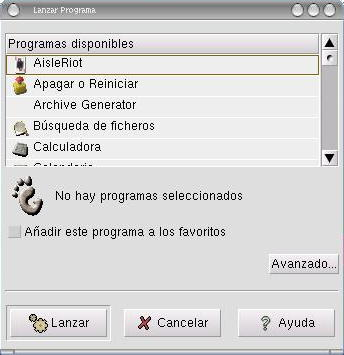
\includegraphics[width=0.45\textwidth]{imagenes/gnome_lanzar.eps}
\label{gnome_lanzar}}
\subfigure[Cuadro de di�logo avanzado {\tt LANZAR PROGRAMA}]{%
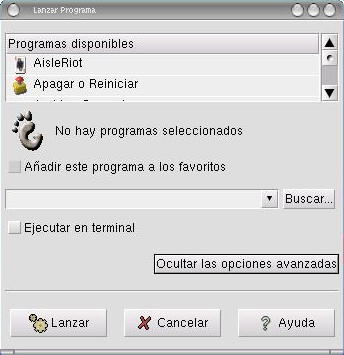
\includegraphics[width=0.45\textwidth]{imagenes/gnome_lanzar_avd.eps}
\label{gnome_lanzar_avd}}
\end{figure}

Manejar  {\sf  GNOME} es  cuesti�n  de  jugar  un  rato y  probar  las
diferentes opciones. Disponemos  de tres botones en  nuestro rat�n (ya
hablamos de  eso en  apartados anteriores) y  se trata  de utilizarlos
sobre los elementos del entorno para ver como reaccionan. Por ejemplo,
si pulsamos  con el bot�n derecho  del nuestro rat�n sobre  alg�n �rea
sin elementos de  algunos de los paneles, veremos un  men� de contexto
similar  al men�  principal del  que  hemos estado  hablando hasta  el
momento.  En el  men�  del  que estamos  hablando  existe un  elemento
denominado {\tt PANEL} que contiene  las opciones de configuraci�n del
panel. Con opciones podemos:

\begin{description}

\item[A�ADIR AL PANEL] Esta opci�n nos permite a�adir nuevos elementos
al  panel.  A  parte  de  los  tipos de  botones  entre  los  que  nos
deja  elegir,  podemos  acceder  a  {\tt  MEN�}  para  a�adir  algunos
de  los  diversos tipos  de  men�s  de aplicaciones.  Tambi�n  podemos
acceder  a  {\tt  LANZADOR  DESDE MEN�}  y  elegir  alguna  aplicaci�n
del  men� principal.  Esto crea  un  bot�n que  lanzar� la  aplicaci�n
autom�ticamente con s�lo pulsar sobre  el mismo. Todos estos elementos
pueden ser movidos, incluso entre paneles, con s�lo pulsar sobre ellos
con  el  bot�n  central.  Tambi�n podemos  modificar  sus  propiedades
pulsando con el bot�n derecho y seleccionando la opci�n adecuada.

\item[CREAR UN PANEL] Nos permite crear diferentes tipos de paneles en
cualquier parte de la pantalla.  Es importante destacar que para mover
un panel  de sitio basta  con pulsar con  el bot�n central  de nuestro
rat�n  en cualquier  �rea descubierta  del panel  que pensamos  mover.
Tambi�n podemos  pulsar sobre  las flechas de  los extremos  del mismo
para ocultarlo, y ampliar de esta manera el �rea de trabajo de nuestro
escritorio.

\item[PROPIEDADES] Con esta opci�n podemos alterar las caracter�sticas
del  panel. Algunas  de esas  caracter�sticas  son el  tipo de  panel,
su  tama�o,  la forma  en  que  le panel  se  oculta,  y la  presencia
de  los  botones  de  escondido.   Adem�s,  bajo  en  nombre  de  {\tt
PROPIEDADES GLOBALES}  se encuentran las opciones  para configurar las
caracter�sticas por defecto para todos los paneles.

\item[EDITAR MENUS] Carga el  {\em editor de men�s}\index{GNOME!editor
de men�s} que nos permite personalizar los men�s de aplicaciones.

\end{description}

\begin{figura}{gnome_apliques}{1}
\caption{Ejemplos de paneles con apliques}
\label{gnome_apliques}
\end{figura}

Uno de los aspectos m�s interesantes del entorno de escritorio de {\sf
GNOME} es la existencia de los {\em apliques}\index{GNOME!apliques} (o
{\em  applets}\index{GNOME!applets}).  Los  apliques no  son  m�s  que
peque�as utilidades  cuya interfaz de  usuario est� confinada  al �rea
del  panel  donde  est� instalado  (Figura  \ref{gnome_apliques}).  Su
instalaci�n es  tan simple  como seleccionar {\tt  PANEL $\rightarrow$
A�ADIR  AL PANEL  $\rightarrow$ APLIQUE}  en  el men�  del panel.  Los
apliques  est�n  clasificados, por  lo  que  debemos desplazarnos  por
las  diferentes categor�as  hasta  que seleccionemos  el que  deseamos
instalar.  Al igual  que el  resto de  los elementos  de los  paneles,
podemos  moverlos utilizando  el  bot�n central  del  rat�n o  podemos
alterar su propiedades utilizando  el bot�n derecho. El comportamiento
exacto  frente a  los  diferentes  uso del  rat�n  sobre los  apliques
dependen de  las preferencias  del programador, por  lo que  puede ser
interesante consular  la ayuda  de cada uno  para aprender  a explotar
todo su potencial.

\subsection{Administraci�n de archivos}

Al igual que los entornos  de escritorio de otros sistemas operativos,
{\sf GNOME} permite la administraci�n sencilla y eficiente de nuestros
archivos.  Dos  son  los  programas  que  habitualmente  nos  podremos
encontrar instalados en {\sf GNOME} y que sirven para esta tarea:

\subsubsection{GNOME Midnight Commander}
\index{GNOME!gmc,GNOME!Midnight Commander}

{\sf Midnight  Commander} naci�  como una  herramienta de  consola que
pretend�a imitar y mejorar en lo  posible a otra conocida utilidad del
mundo  de MSDOS  denominada {\sf  Comandante Norton�}.  Dicha utilidad
simplificaba de forma considerable  todas las tareas de administraci�n
de archivos  (tales como la edici�n,  la copia, la b�squeda,  etc.) al
proporcionar una completa  interfaz en modo texto. Con  el tiempo {\sf
Midnight Commander}  fue portado  al entorno  gr�fico de  {\sf GNOME},
aunque las principales mejoras  siguen desarroll�ndose para la versi�n
de consola que podemos utilizar con s�lo ejecutar el comando {\tt mc}.

{\sf GMC (GNOME  Midnight Commander)} se encarga  de gestionar nuestro
fondo de escritorio como �rea  de trabajo\footnote{En ocasiones y pese
a  que el  {\sf GMC}  est�  instalado el  programa puede  que no  est�
cargado,  y por  tanto  carecemos  de iconos  en  el escritorio.  Para
resolverlo  podemos  lanzar  el  comando {\tt  gmc}  desde  el  cuadro
de  di�logo  {\tt  LANZAR  PROGRAMA}.  Y  a  continuaci�n  seleccionar
{\tt CONFIGURACI�N  $\rightarrow$ SESI�N $\rightarrow$  GUARDAR SESI�N
ACTUAL}  en  el  men�  principal  de {\sf  GNOME}}.  En  ella  podemos
depositar los archivos o directorios que utilicemos habitualmente. Con
s�lo pulsar  con el  bot�n derecho  de nuestro  rat�n sobre  el mismo,
dispondremos  de  todo  un  conjunto  de  opciones  para  organizar  y
configurar nuestro escritorio. Tambi�n podremos crear diferentes tipos
de  nuevos elementos,  como por  ejemplo directorios  o lanzadores  de
aplicaciones.

Al igual  que en otros  entornos gr�ficos, podemos arrastrar  y soltar
los  diferentes elementos  para  moverlos  entre directorios.  Tambi�n
podemos  hacer  una  doble  pulsaci�n  con  el  bot�n  izquierdo  para
abrirlos, o pulsar el bot�n derecho de nuestro rat�n para acceder a un
completo  men�  con  las  acciones  que  podemos  realizar  sobre  los
elementos seleccionados.

\begin{figura}{gnome_gmc}{0.98}
\caption{GNOME Midnight Commander}
\label{gnome_gmc}
\end{figura}

Si elegimos  abrir un directorio,  {\sf GMC} suele  responder abriendo
una ventana similar  a la de la Figura \ref{gnome_gmc}.  En el �rea de
las izquierda  de dicha  ventana disponemos  de una  representaci�n de
todo el  �rbol de directorios  de nuestro sistema, lo  cual simplifica
notablemente  la navegaci�n.  Mientras que  en el  �rea de  la derecha
podemos ver los archivos y/o subdirectorio de directorio seleccionado.
{\sf GMC} nos permite seleccionar  diferentes tipos de vistas para los
archivos, as�  como manipularlos a nuestra  conveniencia utilizando el
rat�n. Nuevamente podemos arrastrar y soltar para mover archivos entre
directorios,  o  podemos utilizar  el  bot�n  derecho del  rat�n  para
seleccionar una de las m�ltiples acciones de las que disponemos.

\subsubsection{Nautilus}
\index{GNOME!Nautilus}

Aunque {\sf  GMC} es  un administrador de  archivos sencillo  y ligero
su  desarrollo est�  pr�cticamente  abandonado. En  su  lugar se  est�
imponiendo el uso  de una aplicaci�n mucho m�s  potente, y visualmente
m�s  atractiva,  denominada  {\sf  Nautilus}. Aun  as�  es  importante
destacar  que {\sf  Nautilus} es  una aplicaci�n  excesivamente pesada
para ordenadores un tanto antiguos y/o escasos de recursos.

\begin{figura}{gnome_nautilus}{0.85}
\caption{Administrador de archivos Nautilus}
\label{gnome_nautilus}
\end{figura}

{\sf Nautilus} pretende ser par {\sf  GNOME} lo que {\sf Konqueror} es
para {\sf KDE}.  Es decir, un administrador de  archivos, un navegador
web  y un  visor de  documentos. Como  podemos observar  en la  Figura
\ref{gnome_nautilus} la disposici�n de  todos los elementos en similar
a la que tenemos  en {\sf GMC}. Es m�s, en lo  que a la administraci�n
de  archivo se  refiere se  comporta  de forma  exactamente igual.  Si
estamos  acostumbrados  a manejar  a  uno  no tendremos  problemas  en
utilizar el otro.

\subsection{Configuraci�n del escritorio}

La  configuraci�n  para  personalizar  nuestros  escritorio  se  puede
realizar  desde  el  {\sf  Centro  de  control}\index{GNOME!Centro  de
control} (Figura \ref{gnome_control}). Para acceder al mismo basta con
seleccionar  {\tt CONFIGURACI�N  $\rightarrow$  CENTRO  DE CONTROL  DE
GNOME} en el men� principal del entorno.

\begin{figura}{gnome_control}{0.85}
\caption{Centro de control GNOME}
\label{gnome_control}
\end{figura}

En la parte derecha de la  ventana contamos con la lista de categor�as
en las que se clasifican  las diferentes opciones de configuraci�n del
entorno de escritorio {\sf GNOME}.  Cuando seleccionamos una de dichas
categor�as  el  lado izquierdo  cambia  para  mostrarnos las  opciones
disponibles.

Cualquier  cambio en  la  configuraci�n puede  ser  validado con  {\tt
ACEPTAR}  o  rechazado  con   {\tt  CANCELAR}.  Sin  embargo,  podemos
comprobar los efectos de esos cambios con s�lo pulsar en {\tt PROBAR}.
El sistema  autom�ticamente se  ajustar� a nuestras  preferencias pero
sin guardar los cambios definitivamente.  Antes de cerrar el centro de
control es  necesario que pulsemos  {\tt ACEPTAR}  en cada una  de las
categor�as, independientemente  de que las  hallamos probado o  no. El
t�tulo de la  categor�a modificada se muestra en  rojo para indicarnos
que todav�a no hemos aceptado o  rechazado los cambios. Por �ltimo, el
bot�n  {\tt REVERTIR}  nos  permite devolver  las  opciones al  estado
anterior al de las modificaciones.

\section{El escritorio de KDE}\index{KDE}

\begin{figura}{pantallazo_kde_descrito}{0.6}
\caption{Aspecto del escritorio KDE}
\label{kde}
\end{figura}

{\sf  KDE} es  entorno de  escritorio  con gestor  de ventanas  propio
basado  en {\sf  X-Window}  que  nos da  un  entorno gr�fico  amigable
para  realizar  las  operaciones  m�s comunes  con  nuestro  ordenador
(Figura  \ref{kde}).   Cuenta  con  un  panel   donde  tener  nuestras
aplicaciones organizadas, un gestor de  archivos y navegador web ({\em
Konqueror}\index{KDE!Konqueror}), y otros  muchos programas para hacer
nuestro trabajo mucho m�s c�modo, o  pasar buenos ratos de ocio frente
al ordenador.

\subsection{Paneles y men�s de KDE}

\begin{figura}{kde_panel}{0.9}
\caption{Panel de KDE y algunos de sus iconos descritos}
\label{kde_panel}
\end{figura}

Al  igual que  en {\sf  GNOME},  en {\sf  KDE} contamos  con un  panel
en  el  que  se  organizan  todos los  men�s  y  aplicaciones  (Figura
\ref{kde_panel}). Este concepto  es familiar en la  inmensa mayor�a de
los gestores  de ventanas  y entornos  gr�ficos que  podamos encontrar
en  cualquier  ordenador.  Este  panel  puede  ser  ubicado  por  toda
la  pantalla, redimensionado,  etc.,  y es  altamente configurable  en
aspecto, tama�o y funcionalidades.

Se puede acceder  a los programas a  trav�s del men� que  se activa al
pulsar sobre el  icono con una {\em K} (Figura  \ref{kde_menuk}), y un
engranaje,  a  la  izquierda  del  panel de  la  parte  inferior.  Los
programas  se distribuyen  en  varios submen�s,  y  se clasifican  por
tipos.  Normalmente, estos  submen�s  suelen tener  t�tulos como  {\tt
PROGRAMAS}, {\tt MULTIMEDIA}, etc\dots

El emulador  de terminal  puede conseguirse en  {\sf KDE}  mediante el
bot�n que aparece en el panel que simboliza un monitor con una peque�a
concha (shell en ingl�s) en  su esquina superior izquierda. No debemos
confundirlo con  el que se  encuentra por defecto inmediatamente  a su
derecha, con  unas barras  de colores  pintadas en  el interior  de un
monitor.  Este es  el que  abre  el centro  de control  de {\sf  KDE},
mediante el  cual podemos  configurar la  totalidad de  los par�metros
gr�ficos, est�ticos, de sonido, de rendimiento, de manejo, etc.

Una de  las combinaciones de teclas  m�s �tiles en {\sf KDE}  es {\tt A-F2},
que  nos muestra  el  cuadro de  di�logo {\tt  EJECUTAR},  en el  cual
podemos indicar  cualquier comando  que queramos ejecutar.  Este mismo
cuadro de di�logo nos da la posibilidad de ejecutar el programa, tanto
como otro usuario, como dentro de una sesi�n del emulador de terminal.
A  esta �ltima  opci�n  se  accede pulsando  el  bot�n {\tt  OPCIONES}
(Figura \ref{kde_ejecutar}).

\begin{figure}[hbtp]
\centering
\subfigure[Men� ``K'' desplegado]{%
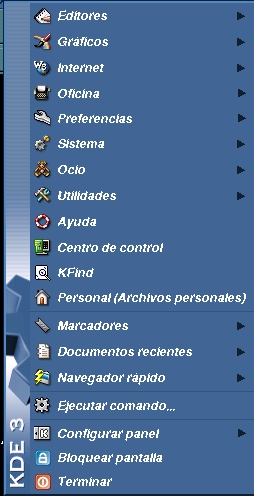
\includegraphics[width=0.49\textwidth]{imagenes/kde_menuk.eps}}
\label{kde_menuk}
\subfigure[Cuadro de di�logo {\tt EJECUTAR} tras pulsar en {\tt OPCIONES }]{%
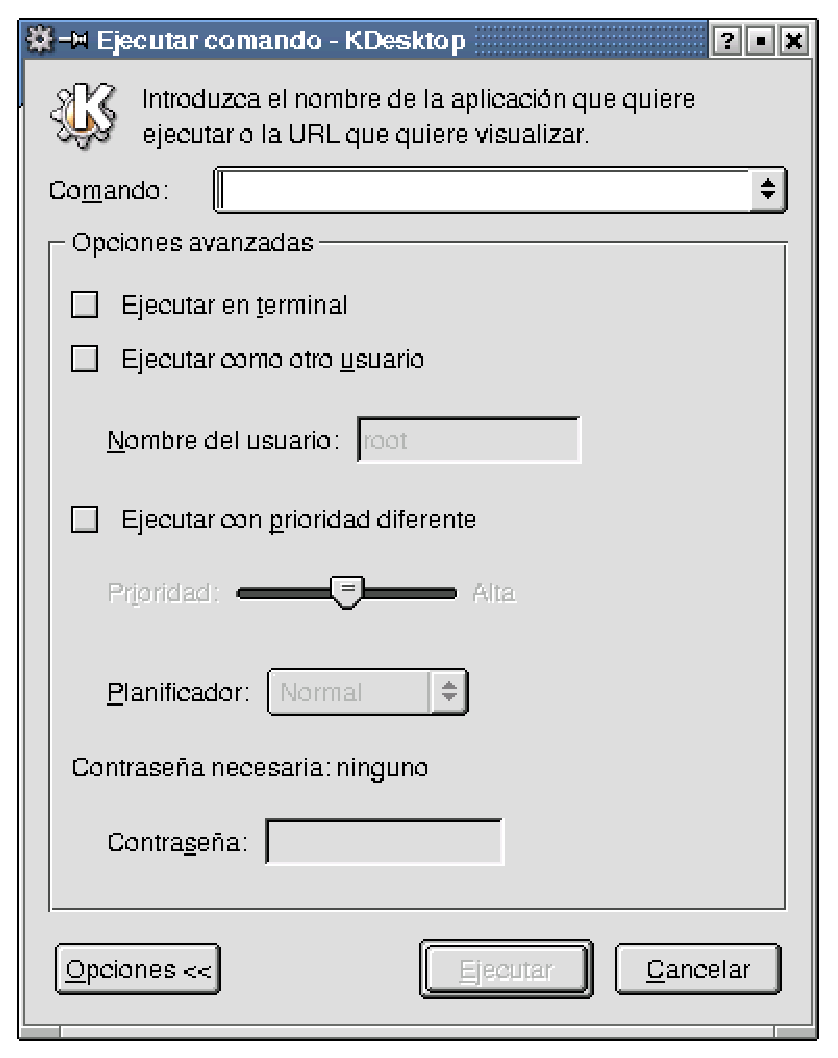
\includegraphics[width=0.49\textwidth]{imagenes/pantallazo_kde_ejecutar.eps}}
\label{kde_ejecutar}
\caption{Men� ``K'' desplegado y cuadro de di�logo {\tt EJECUTAR} tras pulsar en {\tt OPCIONES }}
\end{figure}

Respecto a  las funciones de  los botones del  rat�n en {\sf  KDE}, el
bot�n derecho sobre  el escritorio nos muestra un men�  con unas pocas
opciones,  como crear  nuevos objetos  en nuestro  escritorio (accesos
directos o enlaces, carpetas,etc),  ejecutar comandos, activar men� de
escritorio (lo  cual nos muestra  las opciones del men�  que obtenemos
con el  bot�n derecho, en  la parte  superior de nuestra  pantalla, de
forma permanente.

\subsection{Administraci�n de archivos}

Para  movernos  por  nuestros  archivos, as�  como  para  navegar  por
Internet, {\sf KDE} pone a nuestra disposici�n una potente aplicaci�n:
{\em Konqueror}\index{KDE!Konqueror} (Figura \ref{kde_konqueror_web}).
En   la   barra   de    direcciones   de   dicho   navegador   podemos
poner   tanto  directorios   locales   de   nuestro  ordenador,   como
ubicaciones   FTP   ({\tt   ftp://nombre\_equipo/nombre\_directorio}),
HTTP   ({\tt   http://nombre\_equipo/nombre\_directorio}   e   incluso
carpetas     compartidas     de      Microsoft�     Windows�     ({\tt
smb://nombre\_netbios/carpeta}).

Si  por  ejemplo ponemos  un  directorio  local de  nuestro  ordenador
tal  como {\tt  /home/usuario} (Figura  \ref{kde_konqueror_dir}), {\sf
Konqueror}  muestra un  gestor de  archivos que  dispone de  numerosas
vistas, la posibilidad  de previsualizar archivos de  imagen, etc. Sin
embargo, si  ponemos un recurso  FTP, {\sf Konqueror}  muestra tambi�n
una vista de carpetas, mediante  la cual podemos manejar c�modamente y
de forma  transparente dichos  recursos. Por  ejemplo podemos  subir y
bajar archivos con tan s�lo arrastrar y soltar.

Para arrancar {\sf Konqueror}, debemos pulsar en el icono con un globo
terr�queo  y  un  engranaje  situado  en  nuestro  panel  (ver  Figura
\ref{kde_panel}).

\begin{figura}{kde_konqueror_web}{0.55}
\caption{Konqueror como navegador web}
\label{kde_konqueror_web}
\end{figura}

\begin{figura}{kde_konqueror_dir}{0.55}
\caption{Konqueror como gestor de archivos}
\label{kde_konqueror_dir}
\end{figura}

%Autor: _ese
\chapter{El int�rprete de comandos}
\index{Comandos, int�rprete}
\section{�Qu� es un int�rprete de comandos?}

Si  bien  manejarse en  Linux  es  cada vez  m�s  f�cil,  debido a  la
proliferaci�n  de escritorios,  los  comienzos no  siempre fueron  as�
de  f�ciles. De  hecho,  puede  ocurrir que  nos  encontremos con  una
emergencia  en el  que  no  nos quede  m�s  remedio  que trabajar  con
comandos.

Un int�rprete  de comandos tiene el  aspecto de una pantalla  llena de
letras, generalmente  con fondo negro  y letras  blancas, y que  en la
�ltima l�nea inferior, se suele ver lo siguiente:

\begin{verbatim}
[felix@localhost Comandos]$
\end{verbatim}

En  este entorno  es donde  introduciremos  los comandos  con los  que
trabajaremos, y  coloquialmente diremos que estamos  trabajando en una
consola. Estos comandos pueden ser de diferentes clases:

\begin{itemize}
\item Programas ejecutables.

\item Scripts del int�rprete.

\item Scripts  de lenguajes de  script como {\sf Python},  {\sf Perl},
{\sf Tcl}, etc.

\item Macros del int�rprete.
\end{itemize}

Todos  tienen en  com�n que  son ficheros:  al cargar  un programa  en
Linux, se ordena al int�rprete que busque el fichero con el nombre del
programa y  una vez  encontrado, lo  ejecute, si  �ste da  permisos de
ejecuci�n al usuario.

Los comandos tienen el siguiente aspecto:

\begin{verbatim}
[felix@localhost Comandos]$ fdisk
[felix@localhost Comandos]$ lsmod
[felix@localhost Comandos]$ ls
\end{verbatim}

Tambi�n funcionan con opciones:

\begin{verbatim}
[felix@localhost Comandos]$ fdisk -v
[felix@localhost Comandos]$ ls -a -l
[felix@localhost Comandos]$ ls -al
\end{verbatim}

Y con par�metros:

\begin{verbatim}
[felix@localhost Comandos]$ fdisk /dev/hda
[felix@localhost Comandos]$ ls /tmp
[felix@localhost Comandos]$ ls *.txt
\end{verbatim}

Con opciones y par�metros:

\begin{verbatim}
[felix@localhost Comandos]$ rpm -qpl joe-1.0.3.rpm
[felix@localhost Comandos]$ gcc -o suma suma.c
[felix@localhost Comandos]$ ls -al /tmp
\end{verbatim}

Al  ser Linux  un sistema  {\em multitarea}  y {\em  multiusuario}, se
aportan  ventajas que  se  agradecen  incluso en  un  sistema PC  {\em
monousuario}.  Una de  estas ventajas  es  que se  puede trabajar  con
seis  consolas  virtuales, que  es  como  si pudi�ramos  trabajar  con
varias  sesiones  simult�neas, entendiendo  por  sesi�n  el tiempo  de
trabajo  desde que  el usuario  entra  tras identificarse  en el  {\tt
login}\index{login} de entrada  hasta que abandona el  sistema. Lo que
significa realmente que el mismo  usuario puede entrar varias veces al
mismo tiempo.

Para alternar  entre estas  consolas virtuales,  basta con  pulsar las
combinaciones de la teclas {\tt A-F1} a {\tt A-F6}

Si se quiere acceder a una  consola desde un entorno gr�fico, entonces
se pulsan las combinaciones {\tt C-A-F1} a {\tt C-A-F6}

\section{Directorios y nombres de ficheros}

\subsection{Trabajando con directorios.}

\subsubsection{Estructura del �rbol de directorios}

Toda  la informaci�n  (ya  sean  textos, im�genes,  bases  de datos  o
informaci�n para  la configuraci�n  del sistema)  se almacena  en {\em
ficheros}, que a su vez se guardan en {\em directorios}. Con todas las
herramientas y programas existentes se  puede acceder a estos ficheros
para ver su contenido o  modificarlo. En la Figura \ref{arbol} podemos
ver una ejemplo de dicha estructura en �rbol.

\begin{figure}[hbtp]
\centering
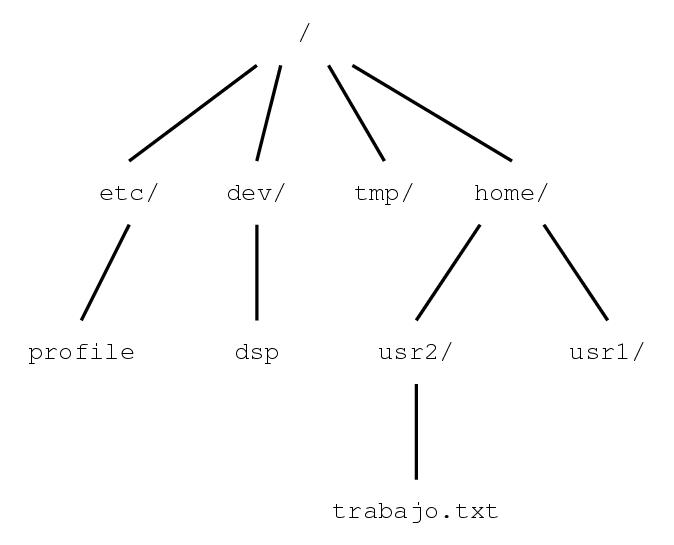
\includegraphics[width=\textwidth]{imagenes/arbol.eps}
\caption{Estructura en �rbol de directorios en sistemas UNIX}\label{arbol}
\end{figure}

Todos los  ficheros y  directorios de  un sistema  UNIX cuelgan  de un
directorio principal  llamado {\em ra�z}\index{directorio  ra�z, ra�z,
/}, que se  representa como {\tt /}. En la  Figura \ref{arbol} podemos
observar como del  directorio ra�z {\tt /}  cuelgan otros directorios,
como {\tt etc} o {\tt home}.

En  dicho  esquema  diferenciamos  los directorios  de  los  ficheros,
complementando el  final del  nombre de los  primeros con  el caracter
{\tt /}.  En el  mismo esquema vemos  como algunos  directorios pueden
contener otros directorios,  como es el caso de {\tt  home}, que es el
{\em padre} de los directorios {\tt usr1} y {\tt usr2}. Tambi�n pueden
contener algunos  ficheros, como es  el caso de  {\tt dev}, que  es el
padre de {\tt  dsp}; o el propio  {\tt usr2}, que es el  padre de {\tt
trabajo.txt}. �ste  �ltimo fichero tiene  la {\em ruta  absoluta} {\tt
/home/usr2/trabajo.txt}, que  define su localizaci�n dentro  del �rbol
de directorios.

Todos  los  directorios  de  un sistema  UNIX  contienen  almenos  dos
subdirectorios.  El  primero es  {\tt  ./}  que representa  al  propio
directorio,  mientras que  el segundo  es  {\tt ../}  y representa  al
directorio padre. Por  ejemplo, el directorio {\tt ./}  dentro de {\tt
/home/usr1} es el propio {\tt  /home/usr1}, mientras que el directorio
{\tt ../}  dentro de  {\tt /home/usr1}  es {\tt  /home}, es  decir, su
directorio padre.

En  los sistemas  UNIX  todo son  ficheros.  Dispositivos como  discos
duros,  scanners  o  disqueteras  se representan  como  {\em  archivos
especiales} en  el directorio  {\tt /dev}. Por  ejemplo, en  la Figura
\ref{arbol} vemos  el fichero {\tt /dev/dsp}  que suele corresponderse
con la tarjeta de sonido instalada en el sistema.

A diferencia de  los sistemas MS-DOS/Windows, en los  sistemas UNIX no
se  reparten los  directorios en  funci�n de  si est�n  en una  unidad
f�sica o en otra (C:, D:, etc.). Durante el arranque del sistema, cada
uno  los  archivos representativos  de  los  diferentes discos  duros,
particiones y  dem�s elementos de  almacenamientos son asociados  a un
directorio  del  directorio  ra�z.  A  este  proceso  se  lo  denomina
{\em  montaje}\index{Montar},  y no  s�lo  es  revesible sino  que  es
completamente configurable.  Por ejemplo, en la  Figura \ref{arbol} el
directorio {\tt /home}  podr�a estar en una partici�n  diferente en un
disco duro distinto al que contiene a  {\tt /} o a {\tt /etc}. Nada en
el esquema  o en  el trabajo  con el sistema  nos permite  apreciar la
diferencia. Por  tanto, no tiene  sentido escribir en la  consola {\tt
C:}, tal  y como har�amos  en MS-DOS. Solamente debemos  dirigirnos al
directorio asociado a esa partici�n que para MS-DOS es {\tt C:}.

Hay que  destacar que  cuando el  usuario accede  a una  sesi�n, Linux
``env�a'' al usuario a su directorio de trabajo. Es decir, si yo entro
como el usuario {\tt felix}, en  el momento de entrar me encontrar� en
el directorio {\tt /home/felix}. �ste  ser� mi directorio personal, en
donde  tengo  libertad absoluta  para  hacer  lo  que quiera  con  mis
ficheros y directorios  ubicados ah�. Sin embargo no  podr� hacer todo
lo que quiera en el directorio  {\tt /home/miguel}. �Por qu�? Pues por
la  sencilla raz�n  de  que Linux  tiene un  sistema  de permisos  que
concede o  restringe libertades sobre  los directorios y  ficheros que
hay en Linux. �Significa eso que  puede existir un usuario ``dios'' en
Linux que puede  hacer totalmente cualquier cosa en Linux?  S�, �se es
el usuario {\tt root}\index{root}. Sin embargo, para los prop�sitos de
este curso,  s�lo nos remitiremos  a la  cuenta de trabajo  del propio
lector ;-)

\subsubsection{Comandos sobre el �rbol de directorios}

Para movernos por el �rbol  de directorios emplearemos el comando {\tt
cd} ({\sf Change Directory}) \index{Comandos!cd}

\begin{verbatim}
[felix@localhost Comandos]$ cd /etc
\end{verbatim}

Es decir, nos vamos al directorio {\tt /etc}

Si  simplemente escribimos  {\tt  cd} sin  especificar  el nombre  del
directorio, esto ser�  igual que escribir {\tt cd  /home/felix} o {\tt
cd}, es decir,  me manda a {\bf mi propio  directorio de trabajo} (que
es como irse a casa).

�C�mo s�  yo en  qu� directorio  me encuentro?  Basta con  escribir el
comando {\tt pwd} ({\sf Print Work Directory}).
\index{Comandos!pwd}
\begin{verbatim}
[felix@localhost felix]$ pwd
/home/felix/
\end{verbatim}

Y la salida que obtendr� es:

\begin{verbatim}
/home/felix
\end{verbatim}

En  caso   de  querer   listar  los   ficheros  y   subdirectorios  de
un   directorio   dado   escribimos   {\tt   ls   nombre\_directorio}.
\index{Comandos!ls}

\begin{verbatim}
[felix@localhost apuntes]$ ls /home/felix/apuntes/apuntes/
Apuntes_CILA_2001.dvi   CVS/    introduccion.sgml  programando.sgml
 xwindow.sgml
Apuntes_CILA_2001.sgml  editores.sgml  LEEME             recursos.sgml
cabecera.sgml           final.sgml     Makefile
 resumen_temario.txt
comandos.sgml           graficos.sgml  matematicas.sgml  sobre.sgml
compila*                internet.sgml  presentacion.sgml temario.estado
\end{verbatim}

El comando {\tt ls} admite par�metros tales como {\tt -a, -l}

\begin{verbatim}
[felix@localhost Comandos]$ ls -a -l
[felix@localhost Comandos]$ ls -al
[felix@localhost Comandos]$ ls -la
\end{verbatim}

Obs�rvese que ambas  formas de escribir los  par�metros son igualmente
v�lidas.  Como anotaci�n,  si queremos  ver que  par�metros se  pueden
utilizar  en   un  comando,   normalmente  basta  con   escribir  {\tt
nombre\_comando --help}.

\begin{verbatim}
[felix@localhost apuntes]$ ls --help
Modo de empleo: ls [OPCI�N]... [FICHERO]...
Muestra informaci�n acerca de los FICHEROs (del directorio actual por defecto).
Ordena las entradas alfab�ticamente si no se especifica ninguna de las
opciones -cftuSUX ni --sort.

Los argumentos obligatorios para las opciones largas son tambi�n obligatorios
para las opciones cortas
  -a, --all                  do not hide entries starting with .
  -A, --almost-all           do not list implied . and ..
      --author               print the author of each file
  -b, --escape               print octal escapes for nongraphic characters
      --block-size=TAMA�O    utiliza bloques de TAMA�O bytes
  -B, --ignore-backups       no muestra la entradas que terminan con ~
  -c                         con -lt: ordena por ctime y muestra ctime (fecha
                               de �ltima modificaci�n del fichero)
                               con -l: muestra ctime y ordena por nombre
                               en cualquier otro caso: ordena por ctime
  -C                         muestra las entradas por columnas
      --color[=CU�NDO]       especifica si se usar� color para distinguir los
                               tipos de ficheros. CU�NDO puede ser `never',
                               `always' o `auto'
  -d, --directory            muestra las entradas de los directorios en lugar
                             de sus contenidos
  -D, --dired                genera el resultado para el modo `dired' de Emacs
  -f                         no ordena, utiliza -aU, no utiliza -lst
  -F, --classify             a�ade un indicador (uno de */=@|) a las entradas
      --format=PALABRA       across -x, commas -m, horizontal -x, long -l,
                               single-column -1, verbose -l, vertical -C
      --full-time            como -l --time-style=full-iso
  -g                         como -l, pero no muestra el propietario
  -G, --no-group             no muestra la informaci�n del grupo
  -h, --human-readable       muestra los tama�os de forma legible
                             (p.e. 1K 234M 2G)
      --si                   an�logo, pero utilizando potencias de 1000,
                             no de 1024
  -H, --dereference-command-line  sigue los enlaces simb�licos en la l�nea de
                                  �rdenes
      --indicator-style=PALABRA  a�ade un indicador con estilo PALABRA a los
                                 nombres de las entradas: none (predeterminado),
                                 classify (-F), file-type (-p)
  -i, --inode                muestra el n�mero de nodo-i de cada fichero
  -I, --ignore=PATR�N        no lista las entradas que coincidan (encajen)
                             con PATR�N de shell
  -k                         como --block-size=1K
  -l                         utiliza un formato de listado largo
  -L, --dereference          al mostrar la informaci�n de un fichero para un
                               enlace simb�lico, muestra la informaci�n del
                               fichero al que apunta el enlace en lugar de la
                               del propio enlace
  -m                         rellena el ancho con una lista de entradas
                             separadas por comas
  -n, --numeric-uid-gid      como -l, pero muestra los UIDs y GIDs num�ricos
  -N, --literal              muestra los nombres literalmente (no trata p.ej.
                             los caracteres de control de forma especial)
  -o                         como -l, pero no muestra el grupo
  -p  --file-type            a�ade un indicador (uno de /=@|) a las entradas
  -q, --hide-control-chars   imprime ? en lugar de los caracteres no gr�ficos
      --show-control-chars   muestra los caracteres no gr�ficos tal y como
                             son (predeterminado a menos que el programa sea
                             `ls' y la salida sea un terminal)
  -Q, --quote-name           encierra los nombres de las entradas entre
                             comillas
      --quoting-style=PALABRA  utiliza el estilo de cita PALABRA para los
                               nombres de las entradas:
                               literal, locale, shell, shell-always, c, escape
  -r, --reverse              invierte el orden, en su caso
  -R, --recursive            muestra los subdirectorios recursivamente
  -s, --size                 muestra el tama�o de cada fichero, en bloques
  -S                         ordena los ficheros por tama�o
      --sort=PALABRA         extension -X, none -U, size -S, time -t, version -v
                             status -c, time -t, atime -u, access -u, use -u
      --time=PALABRA         muestra la fecha seg�n PALABRA, en lugar de la
                             fecha de modificaci�n:
                               atime, access, use, ctime � status; utiliza
                               la fecha especificada como clave de ordenaci�n
                               si --sort=time
      --time-style=PALABRA   muestra la fecha utilizando el estilo PALABRA:
                               full-iso, iso, locale, posix-iso, +FORMATO
                             FORMATO se interpreta como en `date'; si FORMATO
                             es FORMATO1<nueval�nea>FORMATO2, FORMATO1 se
                             aplica a los ficheros no recientes y FORMATO2
                             a los ficheros recientes
  -t                         ordena por la fecha de modificaci�n
  -T, --tabsize=COLS         establece los topes de tabulaci�n a cada COLS
                             en lugar de 8
  -u                         con -lt: ordena por atime y muestra atime (fecha
                               de �ltimo acceso al fichero)
                               con -l: muestra atime y ordena por nombre
                               en cualquier otro caso: ordena por atime
  -U                         no ordena; muestra las entradas en el orden del
                             directorio
  -v                         ordena por versi�n
  -w, --width=COLS           establece el ancho de la pantalla en lugar del
                             valor actual
  -x                         muestra las entradas por l�neas en vez de por
                             columnas
  -X                         ordena alfab�ticamente por la extensi�n de la
                             entrada
  -1                         muestra un fichero por cada l�nea
      --help     muestra esta ayuda y finaliza
      --version  muestra la versi�n y finaliza

TAMA�O puede ser (o puede ser un entero seguido opcionalmente por) uno
de los siguientes: kB 1.000, K 1.024, MB 1.000.000, M 1.048.576, y as�
en adelante para G, T, P, E, Z, Y.

Por defecto, no se emplea color para distinguir los tipos de ficheros. Esto
equivale a usar --color=none. Usar la opci�n --color sin el argumento opcional
CU�NDO equivale a usar --color=always. Con --color=auto, s�lo se muestran
los c�digos de color si la salida est�ndar est� conectada a un terminal (tty).

Comunicar bichos a <bug-fileutils@gnu.org>.
\end{verbatim}

Disculpe el  lector semejante ejemplo, pero  era para que se  viera la
informaci�n que se  puede obtener de primera mano.  Para consultar con
detenimiento esta  ayuda, el  autor recomienda usar  {\tt ls  --help |
more}, y  que seg�n se  avanza con la  informaci�n, se pulsa  la barra
espaciadora, y para salir, se pulsa la tecla {\tt q}.

Obs�rvese que  se pueden  escribir los par�metros  de dos  formas: una
corta ({\tt -l, -a}) y otra larga ({\tt --all, --help}).

Para crear  un directorio, usaremos {\tt  mkdir nombre\_directorio}.

\begin{verbatim}
[felix@localhost apuntes]$ mkdir pepe
[felix@localhost apuntes]$ mkdir tmp
\end{verbatim}

Mientras que para eliminarlo  usaremos {\tt rmdir nombre\_directorio}.
{\bf �Atenci�n! El directorio que  se quiere eliminar debe estar vac�o
y no debe haber nadie trabajando en �l en ese momento.} Evidentemente,
podemos crear y  destruir un directorio dando su ruta  completa o s�lo
su nombre si nos encontramos en el directorio que lo contiene. En caso
de querer  borrar de un s�lo  golpe un directorio y  todo su contenido
disponemos del comando {\tt rm} con las opciones {\tt -rf}. {\bf Mucho
cuidado con borrar  directorios enteros sin comprobar lo  que se hace,
pues no sue�e haber forma de recuperar los archivos borrados}

\begin{verbatim}
[felix@localhost apuntes]$ rmdir pepe
[felix@localhost apuntes]$ rm -rf tmp
\end{verbatim}

Obs�rvese que los comandos  anteriores borran los subdirectorios {\tt
pepe} y {\tt tmp} del directorio actual. Como hemos comentado, podemos
emplear rutas absolutas  para crear o borrar  un directorio cualquiera
del �rbol de directorios.

\begin{verbatim}
[felix@localhost apuntes]$ mkdir /home/felix/pepe
[felix@localhost apuntes]$ rmdir /home/felix/pepe
\end{verbatim}

\subsection{Trabajando con ficheros}

\subsubsection{Comandos sobre el �rbol de ficheros}

El  comando  para  copiar  un   fichero  es  {\tt  cp  fichero\_origen
fichero\_destino}, es decir, que copiamos el fichero {\tt pepe.txt} en
{\tt juan.txt}.

\begin{verbatim}
[felix@localhost apuntes]$ cp pepe.txt juan.txt
\end{verbatim}

El   comando  para   mover  o   renombrar  un   fichero  es   {\tt  mv
fichero\_origen fichero\_destino},  es decir, que copiamos  el fichero
{\tt pepe.txt} en {\tt juan.txt},  pero {\tt pepe.txt} deja de existir
f�sicamente.

\begin{verbatim}
[felix@localhost apuntes]$ mv pepe.txt juan.txt
\end{verbatim}

\noindent\rule{\linewidth}{.75pt}  NOTA:  El  int�rprete  de  comandos
\textbf{S�} distingue en may�sculas y  min�sculas, tanto en el caso de
los comandos como en el de  los ficheros y directorios. Esto significa
que el comando mv es totalmente diferente  a {\tt Mv}, {\tt mV} y {\tt
MV}. Asimismo,  el fichero {\tt pepe.txt}  no es el mismo  fichero que
{\tt Pepe.txt}, ni que {\tt PEPE.TXT}, etc.
\rule{\linewidth}{.75pt}
\vspace{1pt}

En  caso de  que  deseemos borrar  definitivamente  un fichero  podemos
emplear el comando {\tt rm nombre\_fichero}.

\begin{verbatim}
[felix@localhost apuntes]$ rm pepe.txt juan.txt
\end{verbatim}

\subsubsection{Utilizaci�n de comodines}

En ocaciones el  nombre de los directorios y/o ficheros  sobre los que
estamos trabajando  contienen partes comunes que  podemos utilizar con
ayuda  de  comodines  para  facilitarnos  el uso  de  la  interfaz  de
comandos.

En general el caracter {\tt *} al  indicar el nombre de un fichero y/o
directorio  es sustituido  por  un n�mero  indeterminado de  cualquier
combinaci�n de caracteres. Por ejemplo,

\begin{verbatim}
[felix@localhost apuntes]$ rm pe*
\end{verbatim}

\noindent borrar� cualquier  ficheros que empiecen por {\tt  pe} en el
directorio actual. Mientras que,

\begin{verbatim}
[felix@localhost apuntes]$ cp *txt* tmp/
\end{verbatim}

\noindent copiar� los ficheros que contengan la cadena {\tt txt} en el
nombre al directorio {\tt tmp}.

El caracter {\tt ?} al indicar el nombre de un fichero s�lo representa
a {\em un} car�cter cualquiera.

\begin{verbatim}
[felix@localhost apuntes]$ mv pepe?.txt tmp/
\end{verbatim}

El  ejemplo  anterior  mover�  archivos como  {\tt  pepe.txt}  o  {\tt
pepa.txt} al directorio {\tt tmp}.

\subsubsection{Sistema de permisos}

A la hora  de trabajar con ficheros, es necesario  entender el sistema
de  permisos de  los ficheros  y  directorios. Si  escribimos {\tt  ls
-l}\index{Ficheros!permisos,  Ficheros!propietario,  Ficheros!tama�o},
nos encontramos con la siguiente salida: \index{Fichero!permisos}

\begin{verbatim}
[felix@localhost apuntes]$ ls -l
total 468
-rw-rw-r--    1 felix    felix      163004 oct 29 10:05
 Apuntes_CILA_2001.dvi
-rw-rw-r--    1 felix    felix      119151 oct 29 10:05
 Apuntes_CILA_2001.sgml
-rw-rw-r--  1 felix  felix    1617 oct 28 22:15 cabecera.sgml
-rw-rw-r--  1 felix  felix   13329 oct 29 10:05 comandos.sgml
-rwx------  1 felix  felix      33 oct 29 00:32 compila*
drwxrwxr-x  2 felix  felix    4096 oct 28 23:20 CVS/
-rw-rw-r--  1 felix  felix   17250 oct 28 12:11 editores.sgml
-rw-rw-r--  1 felix  felix      12 oct 27 23:10 final.sgml
-rw-rw-r--  1 felix  felix     157 oct 27 23:10 graficos.sgml
-rw-rw-r--  1 felix  felix    2816 oct 28 21:51 internet.sgml
-rw-rw-r--  1 felix  felix   23308 oct 28 23:05 introduccion.sgml
-rw-rw-r--  1 felix  felix     402 oct 27 23:10 LEEME
-rw-rw-r--  1 felix  felix    2295 oct 28 22:19 Makefile
-rw-rw-r--  1 felix  felix   13087 oct 28 17:30 matematicas.sgml
-rw-rw-r--  1 felix  felix     652 oct 28 21:56 presentacion.sgml
-rw-rw-r--  1 felix  felix    34797 oct 28 21:56 programando.sgml
-rw-rw-r--  1 felix  felix      47 oct 28 21:56 recursos.sgml
-rw-rw-r--  1 felix  felix    1320 oct 25 13:35 resumen_temario.txt
-rw-rw-r--  1 felix  felix    4662 oct 28 22:17 sobre.sgml
-rw-rw-r--  1 felix  felix    5247 oct 28 22:19 temario.estado
-rw-rw-r--  1 felix  felix    7417 oct 27 23:10 xwindow.sgml
\end{verbatim}

La primera letra a  la izquierda de cada l�nea nos  indica si se trata
de un fichero (``-'') o un directorio (``d'').

Despu�s nos encontramos con tres  grupos de tres letras (``rwx''), que
seg�n  est�n activados  (la propia  letra, r,w,x)  o desactivados  (un
gui�n,  -)  nos concede  o  deniega  permisos  de lectura  ({\tt  r}),
escritura ({\tt w}) y ejecuci�n ({\tt x}). �Y por qu� son tres grupos?
Pues porque las tres primeras letras se refieren al propio usuario que
es el due�o de esos ficheros, el  segundo grupo se refiere al grupo de
usuario  que  pertenece ese  usuario,  y  el  tercero a  los  usuarios
``extra�os`` o ''ajenos'' al usuario. Por tanto, si leemos


\begin{center}
$-\underbrace{rw-}_{u}\underbrace{rw-}_{g}\underbrace{r--}_{o}$
\end{center}

vemos  que se  trata  de un  fichero  (-) con  permisos  de lectura  y
escritura  para el  usuario y  el grupo  al que  pertenece, y  de s�lo
lectura para un ``extra�o''.

El  siguiente  ser�a un  fichero  de  lectura, escritura  y  ejecuci�n
�nicamente para el usuario pro\-pie\-ta\-rio del fichero.

\begin{center}
$-\underbrace{rwx}_{u}\underbrace{---}_{g}\underbrace{---}_{o}$
\end{center}

Este  �ltimo ejemplo  es un  directorio (d)  con permisos  de lectura,
escritura  y ejecuci�n  para  el  usuario y  el  grupo,  y de  lectura
y  ejecuci�n  para el  ``extra�o''.  En  el  caso de  directorios,  el
permiso de  ejecuci�n es equivalente  a permiso para ``entrar''  en el
directorio.

\begin{center}
$d\underbrace{rwx}_{u}\underbrace{rwx}_{g}\underbrace{r-x}_{o}$
\end{center}

En  el ejemplo  del  listado anterior  vemos dos  veces  el nombre  de
``felix''. El de la primera columna se refiere al usuario propietario,
y el segundo  es el nombre del grupo, que  casualmente coincide con el
nombre  del usuario.  Esto  es importante  recordarlo, porque  debemos
tener  en  cuenta  que  {\bf  jam�s podremos  eliminar  un  fichero  o
retocarlo  si no  tenemos permisos  de  escritura sobre  �l}. Esto  es
impensable en algunas versiones de Microsoft� Windows�.

Si queremos que un fichero cambie de propietario, lo haremos, con {\tt
chown}: \index{Comandos!chown, Ficheros!propietario}

\begin{verbatim}
[felix@localhost apuntes]$ chown miguel pepe.txt
\end{verbatim}

si antes, {\tt pepe.txt} era de {\tt  felix}, ahora pasa a ser de {\tt
miguel}.

De   igual   forma,   para   cambiarlo   de   grupo,   usaremos   {\tt
chgrp}\index{Comandos!chgrp}. Si  {\tt pepe.txt} era del  grupo de los
profesores,  y queremos  que sea  del grupo  de los  estudiantes, s�lo
habr� que escribir lo siguiente:

\begin{verbatim}
[felix@localhost apuntes]$ chgrp estudiantes pepe.txt
\end{verbatim}

En algunos sistemas  no se puede cambiar el propietario  de un fichero
bajo ciertas condiciones:

\begin{verbatim}
$ ls -l hola
-rw-r--r--    1 miguev   108             0 ago 10 20:27 hola
$ chown frodo hola
chown: hola: Operaci�n no permitida
\end{verbatim}

Esto es normal en sistemas donde hay cuotas de usuario. Las cuotas son
un mecanismo de limitaci�n para que  los usuarios no puedan ocupar m�s
de un  determinado volumen (su cuota)  en el disco. Si  este mecanismo
est� activo  no se permite  a los  usuarios cambiar el  propietario de
ning�n fichero, ya que podr�a usarse  este cambio para ocupar la cuota
de otro usuario.

\index{Comandos!chmod, Ficheros!permisos}
Finalmente, para  cambiar los permisos  de un fichero, lo  haremos con
{\tt chmod},  indicando a  que tipo de  usuario queremos  asignarlos y
sobre qu� permisos.  Para indicar el usuario  propietario, usaremos el
par�metro {\tt u}, el  de grupo ser� {\tt g} y el  ajeno ser� {\tt o},
(de {\tt otros}). Para indicar el tipo de permiso, usaremos las letras
{\tt  r},  {\tt w},  {\tt  x},  seg�n  sean  de lectura,  escritura  o
ejecuci�n  respectivamente. Y  para conceder  o denegar,  usaremos los
s�mbolos ``+'' y ``-'':

\begin{verbatim}
[felix@localhost apuntes]$ chmod u+rwx pepe.txt
\end{verbatim}

Este ejemplo sirve para dar todos los permisos al usuario.

En el  siquiente ejemplo  daremos permisos de  lectura y  ejecuci�n al
usuario  y al  grupo,  pero  no de  escritura  sobre  el fichero  {\tt
compila}.

\begin{verbatim}
[felix@localhost apuntes]$ chmod ug+r-x compila
\end{verbatim}

O quitar el permiso de ejecuci�n a  todos los usuarios sin que se vean
afectados los otros tipos de permisos:

\begin{verbatim}
[felix@localhost apuntes]$ chmod -x probar
\end{verbatim}

\section{Comandos b�sicos para sobrevivir}

A  parte de  los comandos  para el  manejo de  ficheros y  directorios
existen  algunos otros  que  conviene conocer  puesto que  simplifican
notablemente nuestro quehacer diario.

\subsection{Teclas especiales}

La interfaz de comandos est� llena de atajos de teclado dise�ados para
facilitarnos  la vida.  La  mayor parte  se  apoyan en  el  uso de  un
historial de los �ltimos comandos ejecutados. Estos son algunos de los
atajos m�s importantes:

\begin{description}

\item[{\tt Teclas del cursor}] Las  flechas hacia arriba y hacia abajo
nos  permiten  elegir  un  comando  de entre  los  almacenados  en  el
historial de la interfaz de comandos. Las flechas hacia la izquierda y
hacia la derecha  nos permiten movernos por la l�nea  de comandos para
editarla.

\item[{\tt TAB}] Si  mientras escribimos el nombre de un  comando o el
de  un  fichero tenemos  alguna  duda  podemos  pulsar {\tt  TAB}.  La
interfaz de comandos nos ayudar� completando el nombre en la medida de
lo posible.  En caso  de que  no sepa darnos  una respuesta  por haber
varias soluciones  disponibles podemos pulsar nuevamente  para que nos
muestre  una lista  de  las mismas.  La interfaz  de  comandos nos  lo
indicar� con una se�al sonora si no hay ninguna soluci�n posible.

\item[{\tt S-Re. Pag. y S-Av. Pag.}] Nos  permiten movernos por el b�ffer de
pantalla de la  consola para ver texto que en  condiciones normales no
podemos observar  puesto que el  desplazamiento vertical lo  ha dejado
fuera de la misma.

\item[{\tt C-l}] Limpiar la pantalla de la consola.

\item[{\tt C-r}] Buscar comandos en el historial.

\end{description}

\subsection{Imprimir en la salida est�ndar}

Uno   de   los  comandos   m�s   pr�cticos   y  utilizados   es   {\tt
cat}\index{Comandos!cat}.   Dicho   comando  encadena   los   archivos
especificados y los imprime por pantalla uno detr�s de otro.

\begin{verbatim}
[felix@localhost apuntes]$ cat pepe.txt juan.txt
\end{verbatim}

En realidad  los comandos de la  consola de GNU/Linux no  entienden la
salida por pantalla y la entrada por  teclado de la misma forma que la
entendemos nosotros. La mayor parte de los comandos toman toda o parte
de la informaci�n que necesitan para  realizar su trabajo de lo que se
denomina la  {\em entrada est�ndar}.  De la misma manera,  utilizan la
{\em salida est�ndar}  para mostrar los resultado de su  trabajo, y la
{\em salida de error est�ndar} para mostrar los mensajes de lo errores
producidos durante la realizaci�n de la misma.

En general la {\em entrada est�ndar} suele estar asociada a la entrada
por teclado, mientras que la {\em salida est�ndar} y la {\em salida de
error est�ndar}  suelen estar sociadas  a la salida por  pantalla. Sin
embargo, Linux nos proporciona mecanismos para que cualquiera de estas
{\em entrada/salidas} pueda ser redirigida a un fichero. De esa manera
la entrada  a un  comando puede haber  sido almacenada  previamente; o
podemos  guardar  la salida  de  un  comando  en  un fichero  para  su
posterior an�lisis.

En  todo caso  la carater�stica  de la  interfaz de  comandos que  nos
interesa es aquella que permite  redirigir la {\em salida est�ndar} de
un comando a la {\em entrada est�ndar} de otro.

\begin{verbatim}
[felix@localhost apuntes]$ cat pepe.txt | sort
[felix@localhost apuntes]$ ls -l | more
\end{verbatim}

En el ejemplo  anterior utilizamos el {\em metacaracter}  {\tt |} para
redirigir la salida del comando {\tt  cat} (es decir, el contenido del
fichero  {\tt pepe.txt})  a  la  entrada del  comando  {\tt sort}.  El
comando {\tt  sort}\index{Comandos!sort} toma las l�neas  de texto que
provienen de la {\em entrada est�ndar},  las ordena, y las muestra por
su  {\em  salida est�ndar}.  Por  lo  tanto,  el ejemplo  muestra  por
pantalla el contenido de {\tt pepe.txt} ordenado alfab�ticamente.

En el mismo ejemplo redirigimos la  salida de {\tt ls} al comando {\tt
more}.  El comando  {\tt more}\index{Comandos!more}  resulta muy  util
cuando el  contenido de  un fichero o  la salida de  un comando  es lo
suficientemente grande como para no  caber completa en la pantalla. En
esos casos  {\tt more} nos permite  ver el texto pantalla  a pantalla,
utilizando la barra espaciadora para avanzar por el mismo.

Un comando  mucho m�s  potente pero  con una  utilidad similar  a {\tt
more} es {\tt less}\index{Comandos!less}.

\begin{verbatim}
[felix@localhost apuntes]$ ls -l | less
\end{verbatim}

El comando {\tt less} nos permite utilizar las teclas del cursor, {\tt
Re. Pag.}  y {\tt Av.  Pag.} para avanzar  y retroceder por  el texto.
Tambi�n  podemos iniciar  una b�squeda,  o continuar  una b�squeda  ya
iniciada, con las teclas {\tt /} y {\tt n} respectivamente. Muchas son
las caracter�sticas de {\tt less},  aunque nos conformaremos con saber
que con  {\tt h} podemos consultar  la ayuda del comando  mientras que
con {\tt q} salimos del mismo.

En general los  comandos que hemos estudiado son  programas de consola
como otros cualquiera. Por lo  tanto pueden ser llamados directamente,
e incluso en muchos casos disponen de opciones de l�nea de comandos.

\begin{verbatim}
[felix@localhost apuntes]$ sort -r pepe.txt
[felix@localhost apuntes]$ less pepe.txt
\end{verbatim}

\subsection{El comando {\tt man}}
\index{Comandos!man}

El comando {\tt  man} es muy �til, ya que  nos dar� mucha informaci�n
sobre la mayor�a de los comandos con los que vamos a trabajar.

\begin{verbatim}
[felix@localhost apuntes]$ man bash
\end{verbatim}

Omitimos  la informaci�n  de salida  ya que  puede ser  muy extensa  e
invita al lector a que lo pruebe �l mismo.

En cualquier  caso, en  el tema \ref{documentacion}  estudiaremos este
comando con m�s detenimiento.

\subsection{El comando {\tt gzip}}
\index{Comandos!gzip}

El comando  {\tt gzip nombre\_fichero} comprime  un fichero utilizando
el algoritmo {\sf Lempel-Ziv}.

\begin{verbatim}
[felix@localhost apuntes]$ gzip pepe.txt
\end{verbatim}

Por regla  general el fichero  desaparece y en  su lugar se  crea otro
comprimido y con el mismo nombre m�s el sufijo {\tt .gz}.

La  descompresi�n  se  realiza  utilizando  la  opci�n  {\tt  -d}.  Es
importante destacar  que, al  igual que  antes, el  archivo comprimido
desaparece para dejar en su lugar la versi�n descomprimida.

\begin{verbatim}
[felix@localhost apuntes]$ gzip -d pepe.txt.gz
\end{verbatim}

Debido a la incomodidad de tener que comprimir/descomprimir para poder
acceder  a la  informaci�n son  muchos  los comandos  que cuentan  con
versiones especialmente dise�adas  para manipular archivos comprimidos
directamente. Es  el caso  de {\tt  zless}\index{Comandos!zless}, {\tt
zgrep}\index{Comandos!zgrep},  {\tt  zcat}\index{Comandos!zcat},  {\tt
zmore}\index{Comandos!zmore}, etc\dots

Pese  a lo  extendido  del uso  de  {\tt gzip}  en  la actualidad  hay
muchos otros  algoritmos con  ratios de  compresi�n mayores.  Por ello
se  han  creado comandos  compatibles,  en  cuanto  a opciones  de  la
l�nea  de  comandos,  con  {\tt   gzip},  pero  que  implementan  esos
otros  algoritmos. Es  el  caso  de {\tt  bzip2}\index{Comandos!bzip2}
y   de   los   comandos  {\tt   bzless}\index{Comandos!bzless},   {\tt
bzgrep}\index{Comandos!bzgrep},   {\tt   bzcat}\index{Comandos!bzcat},
{\tt bzmore}\index{Comandos!bzmore}, etc\dots

\subsection{El comando {\tt tar}}
\index{Comandos!tar}

El  comando {\tt  tar} permite  la  manipulaci�n de  {\em ficheros  de
archivo} en  formato {\sf TAR}.  Dichos ficheros est�n  dise�ados para
almacenar uno  o m�s  ficheros y/o directorios  y toda  la informaci�n
relacionada con  los mismos. Entre  esa informaci�n se  encuentran las
fechas  de acceso  y modificaci�n,  los permisos,  el propietario,  el
grupo,  etc. El  origen del  comando {\tt  tar} se  remonta al  uso de
dipositivos sencuenciales  (como por  ejemplo cintas  magn�ticas) para
almacenar  copias de  seguridad de  los  archivos del  sistema. En  la
actualidad no  es sino  una forma  de empaquetar  en un  �nico archivo
pedazos concretos del �rbol de directorios de nuestro sistema.

Para crear  un archivo {\sf  TAR} basta  con que utilicemos  la opci�n
{\tt -c} seguida por la lista de ficheros y/o directorios que queremos
empaquetar. En general el archivo {\sf TAR} resultante es volcado a la
{\em  salida  est�ndar}.  Puesto  que eso  resulta  poco  pr�ctico  es
habitual utilizar la opci�n {\tt -f} seguida del nombre del fichero de
destino.

\begin{verbatim}
[felix@localhost apuntes]$ tar -cf fichero.tar pepe.txt juan.txt /bin
\end{verbatim}

En el ejemplo  anterior {\tt fichero.tar} almacena  tanto los ficheros
{\tt pepe.txt} y {\tt juan.txt}  como el contenido del directorio {\tt
/bin}.

Los datos almacenados en los  ficheros {\sf TAR} no est�n comprimidos.
Por  ello es  habitual  utilizar  las opciones  {\tt  -z}  o {\tt  -j}
para  que {\tt  tar} pase  el  fichero por  {\tt gzip}  o {\tt  bzip2}
respectivamente, cuando termine de empaquetar los ficheros.

\begin{verbatim}
[felix@localhost apuntes]$ tar -zcf fichero.tar.gz pepe.txt /bin
\end{verbatim}

Para recuperar los ficheros originales se sustituye la opci�n {\tt -c}
por {\tt  -x}, mientras que  para verificar la integridad  del archivo
sin tener que desempaquetarlo se utiliza la opci�n {\tt -t}.

\begin{verbatim}
[felix@localhost apuntes]$ tar -xf fichero.tar
[felix@localhost apuntes]$ tar -zxf fichero.tar.gz
[felix@localhost apuntes]$ tar -ztf fichero.tar.gz
\end{verbatim}

\subsection{El comando {\tt grep}}
\index{Comandos!grep}

Cuando deseamos  localizar un cadena de  texto dentro de uno  o varios
ficheros  solemos  recurrir  al  comando  {\tt  grep}.  Dicho  comando
requiere que  se especifique la cadena  de texto a buscar  seguida del
nombre de  los ficheros en  los que  realizar la b�squeda.  Puesto que
alguno de los  caracteres de la cadena de texto  a buscar pueden tener
alg�n significado especial  para la interfaz de  comandos dicha cadena
suele ir entrecomillada.

\begin{verbatim}
[felix@localhost apuntes]$ grep 'felix' *
[felix@localhost apuntes]$ grep 'CaSa' pepe.txt
\end{verbatim}

Como  se puede  observar, en  el  primer ejemplo  estamos buscando  la
cadena  de  texto \verb|'felix'|  dentro  de  todos los  ficheros  del
directorio actual.

En  general {\tt  grep}  es  sensible a  may�sculas  y min�sculas.  Si
queremos eliminar dicho comportamiento  podemos emplear la opci�n {\tt
-i}.  Tambi�n  podemos pedir  que  nos  indique  donde {\bf  NO}  est�
la  cadena indicada  utilizando  la  opci�n {\tt  -v}.  Por otro  lado
las  b�squedas  pueden  extenderse por  directorios  y  subdirectorios
utilizando la opci�n {\tt -r}.

En realidad  {\tt grep} no  s�lo nos permite utilizar  simples cadenas
para buscar dentro  de los ficheros indicados. El  comandos {\tt grep}
nos permite utilizar {\em expresiones  regulares}. Es decir, dentro de
nuestra cadena de texto podemos utilizar caracteres con un significado
especial con los  que podemos buscar casi cualquier  tipo de expresi�n
entre nuestros archivos. Puesto que las expresiones regulares se salen
completamente  del  alcance de  este  tema  recomendamos consultar  la
p�gina correspondiente del manual.

\begin{verbatim}
[felix@localhost apuntes]$ man grep
\end{verbatim}

\subsection{Otros comandos}

\begin{description}

\item [clear]\index{Comandos!clear}  Limpia la pantalla de  la consola
(tecla {\tt C-l})

\item  [locate]\index{Comandos!locate} Es  la  orden  de b�squeda  m�s
r�pida y sencilla para localizar un archivo.

\item  [reset]\index{Comandos!reset} Si  observamos que  escribimos en
pantalla y no aparece el texto pero al pulsar {\tt ENTER} realmente se
est� escribiendo,  o que  los colores  o los textos  de la  consola se
corrompen,  puede  ser  que  alguna  aplicaci�n  en  modo  texto  haya
finalizado  bruscamente  no restaurando  los  valores  est�ndar de  la
consola  al  salir.  Con  esto  forzamos  unos  valores  por  defecto,
regenerando la pantalla.

\item [top]\index{Comandos!top}  Muestra los procesos que  se ejecutan
en  el  momento  actual,  informando  de los  recursos  que  se  est�n
consumiendo.

\item  [whoami]\index{Comandos!whoami}  El   curioso  nombre  de  este
comando proviene {\em  Who am I?} ({\em �Qui�n soy?}),  que indica que
este comando es capaz de informarnos  del nombre de usuario con que se
entr� en esa consola. Puede parecer  una tonter�a, pero si una persona
entra en dos sesiones,  en una como {\tt root} y  en otra como usuario
normal,  si no  se  sabe  qui�n es  en  ese  momento, podr�an  ocurrir
accidentes catastr�ficos.

\end{description}

\section{Unidades de disco}

Como hemos dicho anteriormente, en  Linux no existen las unidades como
{\tt A:} o {\tt C:}. Para acceder a un disco es necesario primero {\em
montarlo}\index{Montar}, esto  es asignarle un lugar  dentro del �rbol
de directorios del sistema.

Por  ejemplo,  podemos asignar  a  la  disquetera el  directorio  {\tt
/floppy}, al CD-ROM el directorio {\tt /cdrom} o a la grabadora de CDs
el  directorio {\tt  /grabata}.  Normalmente los  directorios para  la
disquetera y el  lector de CD-ROM est�n ya asignados  desde el momento
de instalar el  sistema, aunque se puede cambiar a  voluntad (si somos
{\tt root} ;-).

Para    montar     un    disco    utilizamos    el     comando    {\tt
mount}\index{Montar!mount} indic�ndole como  par�metros el dispositivo
al que queremos acceder, el directorio en el que lo queremos montar, y
el  sistema de  archivos utilizado  para ordenar  la informaci�n.  Sin
embargo,  el  administrador ({\tt  root})  suele  indicar todos  estos
par�metros  en el  fichero {\tt  fichero}, y  los usuarios  tienen que
conformarse montar lo  que {\tt root} les permita. En  nuestro caso el
se�or {\tt root}  ha determinado que los usuarios  s�lo podemos montar
la disquetera en el directorio {\tt /floppy}.

\begin{verbatim}
[miguev@euler apuntes]$ mount /dev/fd0 /floppy
mount: only root can do that
[miguev@euler apuntes]$ mount /floppy
\end{verbatim}

Una vez montado el disquete en  el directorio {\tt /floppy} ya podemos
acceder  y  manipular  sus  ficheros y  subdirectorios  como  m�s  nos
convenga. Desde la  perspectiva del usuario no  hay ninguna diferencia
entre trabajar en ese directorio y trabajar en otro cualquiera.

Pobre de quien  saque el disquete sin desmontarlo. �Por  qu�? Pues por
tres razones:

\begin{enumerate}

\item  Existe el  riesgo de  que perdamos  la informaci�n  que hayamos
grabado en el disquete.

\item Ning�n otro usuario podr� usar la disquetera, al menos hasta que
se reinicie el  ordenador o el {\tt root} tenga  tiempo para forzar el
que la unidad sea desmontanda, lo cual no le har� gracia a nadie.

\item El  Sr. root puede  mosquearse con quien lo  haga, y a  nadie le
conviene tener mosqueado al Sr. root.

\end{enumerate}

Para desmontar el disquete simplemente utilizamos el sencillo comando
{\tt umount}\index{Montar!umount}:

\begin{verbatim}
$ umount /floppy
\end{verbatim}

Como �ltimo ejemplo, hagamos lo siguiente:

\begin{verbatim}
$ mount /floppy
$ cd /floppy
$ umount /floppy
\end{verbatim}

�Verdad que no funciona? Esto se debe a que en el momento de desmontar
la  disketera, {\bf  no debe  haber NADIE  dentro} de  ese directorio.
Recordemos que estamos en un  sistema multiusuario y puede ocurrir que
m�s  de  una persona  acceda  a  la  disketera  o a  otro  dispositivo
desmontable, como  el CD-ROM. Por  tanto, hemos de asegurarnos  que no
hay nadie.

Para comprobar en un momento dado  si el disquete est� montado podemos
usar el comando {\tt df}\index{Comandos!df}, que nos informa sobre los
{\em  sistemas  de  ficheros}  que  est�n  montados  y  su  estado  de
almacenamiento.  La opci�n  {\tt  -h} nos  muestra  las cantidades  en
cifras {\em humanas}.

\begin{verbatim}
[miguev@euler apuntes]$ df -h
Filesystem            Size  Used Avail Use% Mounted on
/dev/hda2             1.9G  1.8G   80M  96% /
euler:/home            20G  3.2G   16G  17% /home
euler:/usr/soft       3.9G  5.4M  3.7G   0% /usr/soft
/dev/fd0              1.4M  758k  665k  53% /floppy
\end{verbatim}

Aqu�  vemos  que la  segunda  partici�n  del  primer disco  duro  {\tt
/dev/hda2} est� montada en el directorio {\tt /}, los directorios {\tt
/home} y  {\tt /usr/soft} del  servidor {\tt euler} est�n  montados en
sus equivalente locales, y el  disquete {\tt /dev/fd0} est� montado en
el directorio {\tt /floppy}.

\section{Unidades de disco con Mtools}

En general,  la mayor parte  de los  disquetes que solemos  usar est�n
en  formato  DOS/Windows.  Cuando  disponemos de  uno  esos  disquetes
podemos  acceder  a  su  contenido  de forma  sencilla  con  las  {\sf
Mtools}\index{Mtools}.

{\sf Mtools} es  una colecci�n de herramientas de  dominio p�blico que
permite a sistemas  UNIX manipular ficheros en un  sistema de archivos
DOS/Windows (t�picamente un disquete). {\sf Mtools} es suficiente para
dar acceso  a sistemas de  archivos DOS/Windows. Por  ejemplo, �rdenes
como  {\tt mdir  a:}  funcionan en  el disquete  {\tt  A:} sin  ning�n
montaje preliminar ni otro procedimiento  de inicio (suponiendo que el
{\tt /etc/mtools.conf}  sea correcto). Gracias  a todo ello,  con {\sf
Mtools} uno puede cambiar disquetes sin tener que desmontar y montar.

\subsection{Nombres de ficheros}

Muchas  de  las   herramientas  de  {\sf  Mtools}   requieren  que  se
especifiquen nombres de archivo en  el sistema de archivos DOS/Windows
al que  estamos accediendo.  Las rutas  de ficheros  en el  sistema de
archivos DOS/Windows  se componen de:  una {\em letra  de dispositivo}
seguida de  dos puntos, un subdirectorio  y un nombre de  fichero. Los
nombres de  directorio pueden  emplear como separador  {\tt /}  o {\tt
$\backslash$}. El  uso del  separador {\tt $\backslash$}  requiere que
los nombres se entrecomillen para protegerlos, por lo que recomendamos
utilizar  {\tt /}  con  el fin  de evitar  problemas.  Los nombres  de
ficheros  que  no  van  precedidos  de una  letra  de  dispositivo  se
consideran ficheros del sistema UNIX.

Por ejemplo,  el siguiente  comando copia  el archivo  {\tt TEST1.TXT}
desde  el directorio  {\tt TEST}  del primer  dispositivo de  disquete
({\tt A:}), hasta nuestro directorio  de trabajo actual, con el nombre
de archivo {\tt test2.txt}.\label{mcopyej}

\begin{verbatim}
$ mcopy 'a:\TEST\TEST1.TXT' test2.txt
\end{verbatim}

que es completamente equivalente a:

\begin{verbatim}
$ mcopy a:/TEST/TEST1.TXT test2.txt
\end{verbatim}

Como  es obvio  las  {\sf  Mtools} no  distinguen  entre may�sculas  y
min�sculas  en  el acceso  al  sistema  de archivos  DOS/Windows.  Sin
embargo, si permiten la utilizaci�n de  comodines (como {\tt *} o {\tt
?}) tanto cuando especificamos un nombre de archivo Linux, como cuando
hacemos lo mismo con nombres de archivo DOS/Windows.

En cuanto a  las letras de dispositivo, com�nmente la  unidad {\tt A:}
es la  primera unidad de  disquete, la unidad  {\tt B:} es  la segunda
unidad de disquete,  la unidad {\tt J:}  es una unidad {\em  Jaz} y la
unidad  {\tt Z:}  es  una  unidad {\em  Zip}.  Sin  embargo todo  esto
puede  ser  configurado  mediante  el fichero  de  configuraci�n  {\tt
/etc/mtools.conf}.

\subsection {Lista de comandos}

A continuaci�n presentamos  algunos de los comandos  m�s utilizados de
las {\sf Mtools}.

\subsubsection{mattrib}\index{Mtools!mattrib}

Se emplea para cambiar los  atributos de ficheros DOS/Windows de forma
semejante a como lo hace el comando {\tt ATTRIB} del MS-DOS.

\subsubsection{mcd}\index{Mtools!mcd}

El comando {\tt mcd } se  emplea para cambiar el directorio de trabajo
actual de {\sf Mtools} en los discos DOS/Windows.

\begin{verbatim}
$ mcd <directorio_dos>
\end{verbatim}

Sin argumentos, {\tt mcd} informa de la unidad y directorio de trabajo
actuales. De otra forma, mcd cambia la unidad en curso y el directorio
de trabajo relativos a un sistema de archivos DOS/Windows.

Por ejemplo, si ejecutamos la siguiente secuencia de comandos:

\begin{verbatim}
$ mcd a:/TEST
$ mcopy a:TEST1.TXT test2.txt
\end{verbatim}

Copiar�amos  el  archivo  {\tt  TEST1.TXT}   tal  y  como  lo  hicimos
anteriormente (p�gina \pageref{mcopyej}).

A diferencia de los sistemas DOS/Windows, con {\sf Mtools} s�lo hay un
directorio  de  trabajo  actual  para  todas las  unidades,  y  no  un
directorio de trabajo diferente para cada unidad.

\subsubsection{mcopy}\index{Mtools!mcopy}

El comando {\tt mcopy} permite  copiar ficheros desde o hacia sistemas
de archivos DOS/Windows. Las formas de uso son:

\begin{verbatim} 
$ mcopy fichero_fuente fichero_destino
$ mcopy fichero_fuente <fichero_fuente> directorio_destino
$ mcopy fichero_fuente_dos
\end{verbatim}

El comando copia el {\tt fichero\_fuente} al {\tt fichero\_destino}, o
copia m�ltiples ficheros  al directorio de destino  indicado. Fuente y
destino pueden ser ficheros de DOS o de Linux. La presencia, o no, del
indicador de  letra del dispositivo  es el que determina  que ficheros
son de DOS y cuales de Linux.

Si s�lo  se suministra uno  de los  par�metros fuente, se  supone como
destino el directorio actual de trabajo en el sistema Linux.

\subsubsection{mdel}\index{Mtools!mdel}

El comando {\tt mdel} se emplea para borrar ficheros.

\begin{verbatim}
$ mdel fichero_dos
\end{verbatim}

Por ejemplo:

\begin{verbatim}
$ mdel a:/TEST2.TXT
\end{verbatim}

\subsubsection{mdeltree}\index{Mtools!mdeltree}

El  comando  {\tt  mdeltree}  se utiliza  para  borrar  un  directorio
DOS/Windows y todos sus archivos y subdirectorios.

\begin{verbatim}
$ mdeltree directorio_dos
\end{verbatim}

\subsubsection{mdir}\index{Mtools!mdir}

El  comando {\tt  mdir}  se emplea  para mostrar  el  contenido de  un
directorio DOS/Windows.

\begin{verbatim}
$ mdir <directorio_dos>
\end{verbatim}

Por ejemplo:

\begin{verbatim}
$ mdir a:
 Volume in drive A has no label
 Volume Serial Number is 3E48-13E9
Directory for A:/

TRABAJO  TXT     13838 11-01-1993   3:11
PROGRA~1 EXE    268232 12-14-2002  22:15  programinstall.exe
TEST         <DIR>     12-14-2002  22:13
        3 files             282 070 bytes
                          1 174 528 bytes free
\end{verbatim}

\subsubsection{mformat}\index{Mtools!mformat}

El comando {\tt mformat} se utiliza  para crear un sistema de archivos
DOS/Windows vacio en la unidad indicada.

\begin{verbatim}
$ mformat <unidad:>
\end{verbatim}

\subsubsection{mmd}\index{Mtools!mmd}

El comando  {\tt mmd} se emplea  para crear un nuevo  directorio en un
sistema  de archivos  DOS.  El comando  informar� de  un  error si  el
directorio ya existe.

\begin{verbatim}
$ mmd directorio_dos
\end{verbatim}

\subsubsection{mmove}\index{Mtools!mmove}

El comando {\tt  mmove} se utiliza para mover o  renombra un fichero o
subdirectorio  existente en  un sistema  de archivos  DOS/Windows. Las
formas de uso son:

\begin{verbatim} 
$ mmove fichero_fuente fichero_destino
$ mmove fichero_fuente <fichero_fuente> directorio_destino
$ mmove directorio_fuente directorio_destino
\end{verbatim}

\subsubsection{mrd}\index{Mtools!mrd}

El comando {\tt mrd} se emplea para borrar un directorio de un sistema
de  archivos  DOS/Windows. El  comando  volver�  con  un error  si  el
directorio no existe o no est� vac�o.

\begin{verbatim}
$ mrd directorio_dos
\end{verbatim}

\subsubsection{mtype}\index{Mtools!mtype}

El  comando  {\tt mtype}  muestra  el fichero  DOS/Windows
especificado, en la pantalla o en la salida est�ndar.

\begin{verbatim}
$ mtype fichero_dos
\end{verbatim}

%Autor: Sin asignar

\chapter{Usando Internet}

\section{Navegadores web}

\subsection{Netscape Communicator 4 }
      

Durante   algunos  a�os,   Netscape   ha  sido   el  �nico   navegador
multiplataforma real, dando  cobertura a muchos de  los distintos Unix
comerciales existentes.  Casi desde que Linux  tiene interfaz gr�fico,
ha  existido una  versi�n  del navegador  Netscape  para este  sistema
operativo.


{\em Netscape  Communicator 4} proporciona soporte  para navegaci�n de
p�ginas web  con JavaScript y  Flash 5, permite  visualizar documentos
PDF  dentro del  navegador  (mediante  un plugin  para  el {\em  Adobe
Acrobat Reader}). Tambi�n nos  permite gestionar el correo electr�nico
y componer p�ginas web.



Los  Linuxeros siempre  hemos  considerado que  el navegador  Netscape
consum�a  demasiados  recursos en  Linux,  adem�s  de tener  bastantes
problemas  de  estabilidad.   Debido  a  �ste,  y   a  otros  factores
importantes, como fueron la forma  de competir con las casa Microsoft,
Netscape lleg� a la sana conclusi�n de que la mejor manera de mantener
su navegador en el mercado, era  liberando su c�digo fuente. As� naci�
{\bf Mozilla}


Como debe ser,  dentro de la comunidad del Software  Libre, se alzaron
voces  en  contra  de  ese desperdicio  de  recursos,  proponiendo  la
creaci�n  de navegadores  alternativos. Aqu�  listamos algunas  de las
alternativas que podemos  encontrar en el �rea de  los navegadores web
dentro del Software Libre:

\begin{itemize}
\item{\bf chimera2} - Navegador web para las X
\item{\bf communicator} - Netscape Communicator 4.77
\item{\bf dillo} - Navegador web basado en las GTK
\item{\bf encompass} - Un navegador libre para GNOME
\item{\bf galeon} - Navegador basado en Mozilla, con el aspecto y la
apariencia de las aplicaciones GNOME
\item{\bf konqueror} - El gestor de ficheros, navegador web y visor de
documentos del KDE
\item{\bf links} - Navegador web en modo c�racter
\item{\bf lynx} - Navegador web en modo c�racter
\item{\bf mozilla} - Un navegador Open Source para las X's. Es el heredero
de Netscape.
\item{\bf OpenOffice} - Suite ofim�tica que incluye un buen navegador web
\item{\bf w3m} - Visor web con un excelente soporte para tablas y marcos
\end{itemize}

Bueno, seguro que en el momento  de leer este apartado, habr�n surgido
nuevos navegadores web dentro del mundillo del Software Libre



\section{Transferencia de ficheros (FTP)}


FTP  (File Transfer  Protocol) es  un  protocolo que  se utiliza  para
transferir informaci�n, almacenada en  ficheros, de una m�quina remota
a  otra local,  o viceversa.  Para  poder realizar  esta operaci�n  es
necesario conocer la {\em direcci�n IP} (o el ``nombre'') de la
m�quina a  la que nos  queremos conectar  para realizar alg�n  tipo de
transferencia. Es fundamental distinguir entre m�quina local y m�quina
remota:

\begin{description}

\item[M�quina local]  Es  aqu�lla desde donde nos  conectamos para hacer
la transferencia, es decir, donde ejecutamos ftp.

\item[M�quina  remota]   Es  aquella  a   la  que  nos  conectamos  para
transferir informaci�n.

\end{description}

\subsection{ Inicio de sesi�n FTP}

Para realizar  transferencias  de ficheros  por protocolo  FTP
se  establecen  conexiones (sesiones)  entre  la  m�quina local  y  la
remota. Estas sesiones comienzan por  la autentificaci�n del usuario y
prosiguen  con las  transferencias.  Finalmente la  sesi�n se  cierra.
Veamos un breve ejemplo. 

\begin{verbatim}
$ ftp euler
Connected to euler.fmat.ull.es.
220 ProFTPD 1.2.0pre10 Server (Debian) [euler.fmat.ull.es]
Name (euler:miguev): 
\end{verbatim}

  El   servidor  nos  preguntar�   un  nombre  de   usuario,  y
seguidamente la contrase�a. El nombre  que daremos debe ser una cuenta
de  usuario v�lida  en el  servidor al  que intentamos  acceder, y  la
contrase�a  l�gicamente debe  ser  correspondiente a  ese  usuario. En
servidores p�blicos  suele  existir una cuenta de  acceso an�nima s�lo
para leer (o tal vez una carpeta donde poner cosas pero no leer). Para
acceder a un FTP  como usuario  an�nimo se  utiliza el  nombre {\em anonymous}
y se proporciona  la  direcci�n  de  correo  electr�nico  como  contrase�a.


 Una vez introducido el nombre  y la contrase�a el servidor nos
recibir�  y  el  programa  cliente  de FTP  nos  mostrar�  un  prompt,
manifestando as� que  est� preparado para ejecutar las  �rdenes que le
demos. A  partir de aqu�  se realizan las maniobras  posibles mediante
los com�ndos de FTP que veremos m�s adelante. 

\begin{verbatim}
$ ftp euler
Connected to euler.fmat.ull.es.
220 ProFTPD 1.2.0pre10 Server (Debian) [euler.fmat.ull.es]
Name (euler:miguev): miguev
331 Password required for miguev.
Password:
230 User miguev logged in.
Remote system type is UNIX.
Using binary mode to transfer files.
ftp&gt;
\end{verbatim}



\subsection{ Comandos del FTP}


El protocolo FTP dispone de unos comandos est�ndares suficientes 
para las operaciones de transferencia de ficheros, de los cuales
vemos a continuaci�n un resumen.


\begin{description}

\item[help]  Proporciona una lista de los comandos del FTP de la m�quina
local

\item[help   comando]    Proporciona   informaci�n  sobre   el   comando
especificado, correspondeinte a la m�quina local

\item[lcd directorio-local]  Para moverse de  un directorio a otro en la
m�quina local

\item[lcd unidad:]   Para cambiar de una  unidad de disco a  otra, en el
caso particular de que la m�quina local esa un PC con Windows o MS-DOS

\item[cd directorio-remoto]  Para moverse de un directorio a otro en la m�quina remota

\item[lls directorio-local]   Para listar el contenido  de un directorio
en la m�quina local

\item[[ls|dir] directorio-remoto] 
Para listar el contenido de un directorio en la m�quina remota

\item[! comando]  Para ejecutar un comando en la m�quina local

\item[delete fichero-remoto]  Para borrar un fichero en la m�quina remota

\item[delete  ficheros-remotos]   Para  borrar  varios  ficheros  en  la
m�quina remota

\item[rmdir directorio-remoto]  Para borrar  un directorio en la m�quina
remota

\item[mkdir directorio-remoto]   Para crear un directorio  en la m�quina
remota

\item[pwd]  Para  saber el directorio en  el que se est�,  en la m�quina
remota

\item[ascii]  Para hacer la transferencia  en formato ASCII (lo hace por
defecto)

\item[binary]   Para  hacer  la  transferencia en  formato  binario,  se
utiliza el comando:

\item[get      fichero-remoto     fichero-local]       Transfiere     el
{\tt fichero-remoto}  desde  la  m�quina  remota a  la  m�quina  local,
guard�ndolo con el nombre {\tt fichero-local} en la m�quina local

\item[mget lista-ficheros-remotos]  Transfiere los ficheros listados desde
la m�quina remota a la m�quina local.

\item[prompt]  (Des)activa el modo  interactivo de las transferencias de
ficheros m�ltiples.

\item[put      fichero-local     fichero-remoto]       Transfiere     el
{\tt fichero-local}  desde  la  m�quina  local  a  la  m�quina  remota,
guard�ndolo con el nombre {\tt fichero-remoto} en la m�quina remota

\item[mput  lista-ficheros-locales]   Transfiere los  ficheros  listados
desde la m�quina local a la m�quina remota.

\end{description}

Obviamente, el comando {\tt ftp} no es el �nico programa cliente
de  FTP disponible.  Existen multitud  de programas  clientes de  FTP,
tanto para GNU/Linux como para  otras plataformas, como p.ej. el gFTP.



\section{Acceso remoto (SSH)}


En muchas ocaciones resulta interesante acceder a una m�quina remota y
trabajar como  si estuvi�ramos  f�sicamente frente  a ella.  Es decir,
hablamos de  poder ejecutar  comandos en dicha  m�quina sin  tener que
trasladarnos  a escribirlos  en  su teclado.  Este  tipo de  servicios
existe desde  los or�genes de  Internet pero siempre ha  entra�ado sus
riesgos dado que  es necesaria la autentificaci�n  remota del usuario.
Para entender  de lo  que estamos  hablando s�lo  es necesario que nos
aproximemos  al servicio  de {\em  TELNET} (cuyo  cliente suele  estar
disponible bajo el comando del mismo nombre).

TELNET\index{TELNET} fue el primer  servicio de acceso remoto dise�ado
para  Internet.  B�sicamente el  comando  {\tt  telnet} toma  nuestras
pulsaciones de  teclado y las trasnmite  por la red hasta  el servidor
TELNET de la m�quina remota a  la que estamos conectados. �ste toma la
salida  a terminal  de la  aplicaciones que  vayamos ejecutando  y las
env�a  a  nuestro cliente  en  la  m�quina  local. Ese  mecanismo  tan
sencillo  resuelve  el problema  del  acceso  remoto; excepto  por  un
peque�o  problema. Toda  la comunicaci�n  se realiza  en texto  plano.
Es  decir,  el texto  se  env�a  tal  cual,  sin mecanismo  alguno  de
compresi�n  y/o encriptaci�n  que altere  las cadenas  de texto.  Todo
lo  que  escribimos (p.ej.  comandos  del  int�rprete de  comandos)  y
recibimos (p.ej. correo, informes, cartas) puede ser visto por quienes
intercepten nuestros  paquetes. Esto es especialmente  cr�tico durante
el  proceso de  conexi�n, momento  en  el que  debemos enviar  nuestro
nombre de usuario y contrase�a para realizar la autentificaci�n remota
a la que aludimos anteriormente. Es  evidente que en esa etapa nuestra
password, y  con ella  el acceso  al servidor  bajo nuestro  nombre de
usuario, queda al descubierto.

A   efectos  pr�cticos   la   mayor  parte   de   los  protocolos   de
Internet  se  fundamentan en  TELNET.  Servicios  como la  World  Wide
Web  (HTTP\index{HTTP}),  el   correo  electr�nico  (SMTP\index{SMTP},
POP\index{POP},  IMAP\index{IMAP}),  las  transferencias  de  ficheros
(FTP\index{FTP}), la administraci�n de la red (SMNP\index{SMNP}), etc.
utilizan  protocolos  cuyas  especificaciones  indican  claramente  su
v�nculo con TELNET. Si ya resulta  grave que en todas esas situaciones
nuestros datos queden al descubierto, m�s lo es aun cuando hablamos de
permitir o  denegar el  acceso a  un servicio tan  cr�tico como  es el
acceso remoto. �ste suele poner las  cosas m�s faciles que ning�n otro
para quien desee atacar el sistema.

Dos son las cosas que debemos recordar de todo lo anterior:

\begin{itemize}

\item {\bf  En condiciones normales  la mayor  parte de los  datos que
enviamos y/o  recibimos de Internet  est�n al descubierto.}  Es decir,
una  vez interceptados  pueden  ser le�dos  directamente sin  requerir
ning�n proceso intermedio.

\item  {\bf  No debemos  utilizar  TELNET  bajo ning�n  concepto.}  El
comando {\tt telnet} puede ser una herramienta muy pr�ctica en algunos
casos, pero peligrosa si la usamos para acceso remoto.

\end{itemize}

La  cuesti�n  ahora  es  c�mo podemos  resolver  estos  problemas.  La
respuesta  es  utilizando  {\em Secure  Shell  (SSH\index{SSH})}. Este
programa trabaja de forma similar  a TELNET solo que encriptando tanto
la informaci�n que  es transmitida a la m�quina remota  como la que es
enviada por �sta. El resultado es que aunque la comunicaci�n pueda ser
interceptada los  datos resultar�n ininteligibles. En  realidad SSH es
un  paquete de  comandos  relacionados con  las transacciones  seguras
de  informaci�n en  la  red, que  utiliza  diferentes mecanismos  para
garantizar esa seguridad. De todos  ellos el comando {\tt ssh} esconde
el  programa de  acceso  remoto  del cual  la  forma  m�s sencilla  de
utilizarlo es:

\begin{verbatim} 
$ ssh <usuario>@m�quina_remota 
\end{verbatim}

Por  ejemplo si el  usuario {\tt miquev} quiere  acceder al servidor
{\tt euler.fmat.ull.es} ejecutar�a lo siguiente: 

\begin{verbatim} 
$ ssh miguev@euler.fmat.ull.es 
\end{verbatim}

La primera vez que accedamos a una m�quina el programa nos mostrar� su
{\em huella dactilar} y pedir� que confirmemos que queremos establecer
la conexi�n. Esto  permite utilizar pol�ticas de seguridad  en las que
podamos  verificar  la  autenticidad  de  la  m�quina  a  la  que  nos
conectamos,  evitando  que  pueda  haber  sido  suplantada  por  otra.
Si  estamos seguros  de  la autenticidad  del  sistema remoto  debemos
contestar que  s�. La huella dactilar  es almacenada y vinculada  a la
direcci�n de la  maquina remota, por lo que nunca  m�s recibiremos una
mensaje de verificaci�n  como el anterior. Exceptuando el  caso en que
la m�quina haya cambiado, y con  ello su huella dactilar, situaci�n en
la que probablemente estemos ante una posible suplantaci�n. Si todo va
bien {\tt  ssh} nos  pedir� la  password del usuario.  En caso  de ser
autentificados dispondremos de  acceso remoto sobre el  sistema. Si al
ejecutar el  comando no especificamos  el nombre de usuario  ({\tt ssh
euler.fmat.ull.es}) el  programa utilizar� por defecto  nuestro nombre
en la m�quina local.

A la  hora de trabajar  con {\tt ssh}  debemos tener algunas  cosas en
cuenta. En  caso de  duda podemos  recurrir a  las p�ginas  del manual
({\tt  man ssh})  donde encontraremos  detallada informaci�n  as� como
referencias  a  las  otras  herramientas del  paquete  SSH.  Si  acaso
destacar que debido a que el car�cter {\tt \~{} } tiene un significado
especial  para el  {\tt ssh},  si  queremos escribirlo  en la  m�quina
remota tendremos que pulsar {\tt \~{}\~{} } en nuestro teclado.

Aunque {\tt ssh} garantiza el  acceso remoto seguro no proporciona por
s� solo la  transferencia segura de archivos. Para ello  se utiliza el
comando {\tt scp}\index{scp} que tiene la siguiente forma:

\begin{verbatim}
$ scp <usuario>@<m�quina_origen>:<archivo_origen>;
      <usuario>@<m�quina_destino>:<archivo_destino>;
\end{verbatim}

El  cual copia  {\tt archivo\_origen}  desde la  {\tt m�quina\_origen}
hasta el {\tt archivo\_destino} en la {\tt m�quina\_destino}. Si no se
especifica alguno  de los nombres de  m�quina, el {\tt scp}  asume que
estamos  hablando  del  sistema  local.  El  siguiente  comando  copia
el  archivo  {\tt  mi\_archivo}  desde la  m�quina  local  hasta  {\tt
euler.fmat.ull.es}:

\begin{verbatim}
$ scp mi_archivo euler.fmat.ull.es:
\end{verbatim}

Mientras que el siguiente comando hace lo contrario:
      
\begin{verbatim}
$ scp euler.fmat.ull.es:mi_archivo .
\end{verbatim}

Si al especificar  la ruta de archivo en la  m�quina remota lo hacemos
de forma  relativa (o sea  sin usar {\tt /})  la ruta ser�  relativa a
nuestro directorio personal en la maquina remota. O sea que el comando
anterior copia {\tt mi\_archivo}  desde nuestro directorio personal en
{\tt  euler.fmat.ull.es}. Sin  embargo, el  siguiente comando  copia el
fichero {\tt /tmp/mi\_archivo} (ruta absoluta) en el mismo servidor.

\begin{verbatim}
$ scp euler.fmat.ull.es:/temp/mi_archivo .
\end{verbatim}

Otro comando interesante es {\tt sftp}\index{sftp} que nos proporciona
los  mismos servicios  que {\tt  ftp} solo  que de  forma segura.  Sin
embargo a�n no est� disponible en todos los sistemas.

Una de  las preguntas  m�s habitules  de los usuarios  de Linux  es si
pueden acceder a  su servidor SSH en Linux desde  una m�quina local en
otro  sistema operativo.  La  respuesta  es que  SSH  es un  protocolo
est�ndar por  lo que todo  depende de  la disponiblidad de  un cliente
para su plataforma. En la  actualidad existen versiones libres para la
mayor  parte  de  sistemas  operativos. De  entre  ellas  destacaremos
{\em  PUTTY}[pag. \pageref{putty}]  como uno  de los  mejores clientes
TELNET/SSH para sistemas Microsoft� Windows�.


\section{Correo electr�nico}

\subsection{Mutt }


       Mutt  es un programa  cliente de correo  electr�nico, lo
      que en  ingl�s se denomina  un MUA  (Mail User Agent,  agente de
      correo del  usuario). Es un programa  ``de consola'', lo
      que  significa  que no  necesita  un  entorno de  ventanas  para
      ejecutarse. Al igual que  otros programas basados en pulsasiones
      de  teclas,  Mutt  resulta  ser  poco  intuitivo  al  principio.
      Afortunadamente,  se encuentra  traducido  al  castellano y  eso
      ayuda bastante. 

       Vamos a usar mutt  para familirizarnos un poco �l, ver�n
      que es  simple. Abrimos  una ventana de  emulador de  terminal y
      ejecutan el comando {\tt mutt}. 

\begin{verbatim}
      $ mutt
\end{verbatim}

       Si nos fijamos en la  primera l�nea de la pantalla vemos
      que  aparecen listadas  una  serie de  teclas  con sus  acciones
      asociadas, {\tt q:Salir}, para salir, {\tt d:Sup} para suprimir un
      mensaje, etc. Vemos un ejemplo de  uso para hacernos una idea de
      las funciones b�sicas. 

       El  que se haya fijado  en las dos �ltimas  l�neas habr�
      visto que aparece lo siguiente: 

\begin{verbatim}
---Mutt: (ning�n buz�n) [Msgs:0]---(threads/date)-----------------------(all)---
/var/spool/mail/miguev: No existe el fichero o el directorio (errno = 2)
\end{verbatim}

        Esto significa  que mutt  est� buscando  el correo  del
      usuario  en  {\tt /var/spool/mail/miguev}  (en  el  caso  del
      usuario miguev).  No se asusten.  Lo que  pasa es que  el correo
      est� en esa carpeta pero no en el terminal donde est�n sentados,
      sino en  el servidor de  correo. Para  poder usar el  correo con
      Mutt hay que entrar primero en el servidor, lo que podemos hacer
      r�pidamente  con  lo que  ya  sabemos  de  SSH. Entramos  en  el
      servidor y ejecutamos mutt all�: 

\begin{verbatim}
      $ ssh euler.fmat.ull.es
      miguev@10.0.1.2's password: 
\end{verbatim}

       Una vez  dentro del servidor podemos ya  ejecutar mutt y
      utilizar  el correo  directamente  desde el  servidor. Esto  que
      parece  in�til  tiene  su  utilidad. Imagina  que  est�s  en  un
      ordenador en cualquier  lugar del mundo (con  acceso a internet)
      y  quieres  leer tu  correo  en  la  facultad, pero  no  quieres
      baj�rtelo. Utilizas un programa cliente de SSH para entrar en el
      servidor  y desde  dentro usas  el  correo como  si lo  tuvieras
      delante, aunque est�s dentro del servidor. El mayor problema que
      esto  presenta  es  la  lentitud del  protocolo  SSH  cuando  la
      conexi�n es a trav�s de un m�dem de l�nea telef�nica. 

       Ejecutamos el  comando {\tt mutt} y vemos  en el terminal
      un programa casi todas las l�neas vac�as, salvo la primera y las
      dos �ltimas.  Probablemente en el  momento de abrir  mutt por
      primera vez  no veamos  nada interestante,  pero aqu�  tienen un
      ejemplo de una lista de mensajes vista desde mutt. 

\begin{verbatim}
q:Salir  d:Sup.  u:Recuperar  s:Guardar  m:Nuevo  r:Responder  g:Grupo  ?:Ayuda
  43     Oct 27 Teresa Gonzalez (   0)  *>Re: [l-gulic] CILA LLENO
  44     Oct 27 Lucas Gonzalez  (   0)   >cvs
  45     Oct 27 Miguel �ngel Vi (   0) Bienvenido al calendario de la Universida
  46     Oct 28 Teresa Gonzalez (   0) Re: [l-gulic] Cambios en el CVS de CILA
  47     Oct 28 Pedro Gonzalez  (   0)  *>
  48     Oct 28 Carlos de la Cr (   0) La pu~etera introduccion :-)
  49     Oct 28 carlos de       (   0) maldito texto sobre java
  50     Oct 28 frodo@fmat.ull. (   0) MUY IMPORTANTE!!
  51     Oct 28 frodo@fmat.ull. (   0) ahora te llega?
  52     Oct 28 frodo@fmat.ull. (   0) �como no te llegue! ..grrr
  53     Oct 28 Administrador d (   0) Re: instala esto










---Mutt: /var/spool/mail/miguev [Msgs:53 425K]---(threads/date)---------(end)---

\end{verbatim}

 Vamos a enviar un email a  alguien que est� con nosotros en el
aula, de esa forma cada uno  enviamos un correo y recibimos otro. Para
ello pulsamos  la tecla {\tt m} y  veremos como en la  �ltima l�nea nos
pregunta por el destinatario  del mensaje ({\tt To:}>. Introducimos ah�
la direcci�n de email a la que enviaremos el mensaje: 

\begin{verbatim}
To: frodo@fmat.ull.es
\end{verbatim}

 Seguidamante  mutt nos  preguntar� por  el asunto  del mensaje
({\tt Subject:}). Es importante poner un asunto al mensaje, para que el
destinatario  pueda tener  una idea  de qu�  es ese  mensaje antes  de
abrirlo.  En  un  tiempo  en  que el  contagio  de  virus  por  correo
eletr�nico es preocupantemente frecuente,  resulta muy molesto recibir
un mensaje de email sin asunto. 

\begin{verbatim}
Subject: Hola pringao :-P
\end{verbatim}

 Una  vez que  mutt ya  sabe el destinatario  del mensaje  y el
asunto,  ejecuta el  editor que  tengamos  definido en  el fichero  de
configuraci�n {\tt \~/.muttrc}. Editamos el  mensaje que queramos y
salimos del  editor {\bf guardando el mensaje},  importante esto �ltimo
ya que si salimos del editor  sin guardar el mensaje mutt cancelar� el
env�o. Una vez que salimos del  editor mutt est� preparado para enviar
el mensaje, pero nos ofrece la  posibilidad de hacer a�n varias cosas.


\begin{verbatim}
y:Mandar  q:Abortar  t:To  c:CC  s:Subj  a:Adjuntar archivo  d:Descrip  ?:Ayuda
    From: Miguel �ngel Vilela <miguev@fmat.ull.es>
      To: frodo@fmat.ull.es
      Cc:
     Bcc:
 Subject: Hola pringao
Reply-To: Miguel �ngel Vilela <miguev@fmat.ull.es>
     Fcc:
     Mix: <no chain defined>
     PGP: En claro

-- Archivos adjuntos
- I     1 /tmp/mutt-euler-19795-2          [text/plain, 8bit, iso-8859-1, 0,1K] 








-- Mutt: Crear mensaje

\end{verbatim}

 Como podemos  apreciar en el ejemplo,  tenemos varias opciones
con  sus  teclas  asociadas  en  la primera  l�nea.  Para  cambiar  el
destinatario  pulsar�amos  {\tt t}, para  enviar  una  copia a  alguien
pulsar�amos  {\tt c},  para  editar  el mensaje  de  nuevo  pulsar�amos
{\tt e}, etc. Para enviar el mensaje pulsamos {\tt y}. Entonces mutt nos
devolver� a  la primera pantalla,  pero mostrando en la  primera l�nea
informaci�n acerca del env�o del mensaje. Deber�a aparecer

\begin{verbatim}
Mensaje enviado.
\end{verbatim}

 El resto del manejo  b�sico de {\tt mutt} es bastante intuitivo
y  no   presenta  dificultades.  Si  en   cualquier  momento  deseamos
informaci�n  m�s  detallada  hacerca   de  las  opciones  disponibles,
pulsamos {\tt ?}. 

\begin{verbatim}
i:Salir  -:P�gAnt  <Space>:Pr�xP�g  ?:Ayuda 
^B          M |urlview\n           call urlview to extract URLs out of a message
^D          delete-thread          suprimir todos los mensajes en este hilo
^E          edit-type              editar el tipo de archivo adjunto
^F          forget-passphrase      borrar contrase�a PGP de la memoria
<Tab>       next-new               saltar al pr�ximo mensaje nuevo
<Return>    display-message        mostrar el mensaje
^K          extract-keys           extraer claves PGP p�blicas 
^N          next-thread            saltar al pr�ximo hilo
^P          previous-thread        saltar al hilo anterior
^R          read-thread            marcar el hilo actual como le�do
^T          untag-pattern          quitar marca de los mensajes que coincidan   +                                  con un patr�n
^U          undelete-thread        restaurar todos los mensajes del hilo
<Esc><Tab>  previous-new           saltar al mensaje nuevo anterior
<Esc>C      decode-copy            crear copia decodificada (text/plain)
<Esc>V      collapse-all           colapsar/expander todos los hilos
<Esc>b      M /~b                  search in message bodies
<Esc>c      change-folder-readonly abrir otro buz�n en modo de s�lo lectura
<Esc>d      delete-subthread       suprimir todos los mensajes en este subhilo
<Esc>e      resend-message         usar el mensaje actual como base para uno
+                                  nuevo
Ayuda para index                                                       -- (15%) 

\end{verbatim}



\subsection{Kmail }


 Kmail es el programa cliente de correo para KDE, f�cil de usar
y a la vez muy vers�til y  configurable. Dada su facilidad de manejo y
la premura  de tiempo en  el curso  actual, no entraremos  en detalles
sobre su manejo y configuraci�n. S�lo les animaremos a que sean osados
y exploren libremente sus opciones de configuraci�n. 









%% Autores:
%%      lcabrera
%%      li-po

%% Versi�n
%% $Id$

%% Algunas aplicaciones a detallar:
%% gnotepad,acroread, ghostview, gnumeric, gqview, videolan client, xine

\chapter{Aplicaciones diversas}  En este apartado trataremos,  de manera
muy superficial, algunas aplicaciones de uso cotidiano en Linux.

%% Primera  secci�n
\section{Aplicaciones Gr�ficas} Las  aplicaciones  gr�ficas  disponibles
hoy d�a cubren  un amplio abanico de actividades.  Aqu� expondremos solo
unas pocas de ellas.

\subsection{Internet}
\subsubsection*{Gaim}
\subsubsection*{XChat/KVirc}

\subsection{Multimedia}
\subsubsection*{Xine}
%\subsubsection*{Aviplay}

\subsection{Ofim�tica}
%\subsubsection*{Koffice}
\subsubsection*{OpenOffice}

\subsection{Gr�ficos}
\subsubsection*{Gimp}
\subsubsection*{eog}
\subsubsection*{gqview}
\subsubsection*{ghostview}

\subsection{Desarrollo}
\subsubsection*{Glade/Kdevelop}
\subsubsection*{Cervicia/gcvs}
\subsubsection*{Quanta/Bluefish}

\subsection{Editores}
\subsubsection*{AbiWord}
\subsubsection*{Kwrite}
\subsubsection*{gnotepad}
%\subsubsection*{Kwordtrans}

%\subsection{Sistema}
%\subsubsection*{gmemusage}
%\subsubsection*{gr_monitor}

\subsection{Aplicaciones en general}
\subsubsection*{Creaci�n de CD's}
\paragraph*{GCombust}
%\paragraph*{XCDRoad?}
%\paragraph*{KreateCD}
%\paragraph*{Kover}

%\subsubsection*{Por Definir}

%% Segunda secci�n
\section{Aplicaciones no Gr�ficas}

Se  puede  afirmar  que  por cada  aplicaci�n  gr�fica  disponible  en
Linux,  tenemos 50  utilidades  disponibles desde  la terminal.  Estas
aplicaciones son  el verdadero motor  de todos los  sistemas derivados
de  Unix. Con  ellas  se  pueden llevar  a  cabo  infinidad de  tareas
importantes, desde ordenar  cualquier tipo de archivo  de datos, hasta
programar  el  encendido  de  una cafetera  para  cuando  nos  estemos
quedando dormidos. Todas ellas pueden  ser lanzadas desde una terminal
en modo gr�fico, de manera que tambi�n las podemos utilizar desde este
entorno.


%\subsection{Desarrollo}
%\subsubsection*{GCC}
%\subsubsection*{make}
%\subsubsection*{gettext}

%\subsection{Editores}
%\subsubsection*{emacs}
%\subsubsection*{vim}

\subsection{Gr�ficos}
\subsubsection*{ImageMagick}
\subsubsection*{Otros Filtros}

%\subsection{Internet}
%\subsubsection*{iptraf}
%\subsubsection*{ntop}

\subsection{Multimedia}
\subsubsection*{mpg321}
\subsubsection*{aumix}
\subsubsection*{zgv}
\subsubsection*{aatv}

%\subsection{Ofim�tica}
%\subsubsection*{bc}
%\subsubsection*{}

\subsection{Sistema}
\subsubsection*{top}
\subsubsection*{crontab}
\subsubsection*{at}
\subsubsection*{uptime}



% M�dulo II:  Party
% 1. Sistema base (particiones)
% 2. Hardware y kernel (make [menu|x]config && make-kpkg)
% 3. Software para los m�dulos.
% 4. Administraci�n b�sica (adduser, floppy, cdrom, APT)
% 5. Paquetes en fuentes (bajar, compilar, instalar Xine+dvdnav)
% 6. Software adicional (a gusto del consumidor)

% M�dulo III: Edici�n y maquetaci�n de documentos
% 1. Edici�n de gr�ficos (DIA, QCad, The GIMP)
% 2. OpenOffice
% 3. HTML (lenguaje, bluefish, quanta)
% 4. LyX
% 5. LaTeX
\part{Edici�n y maquetaci�n de documentos}
%Autor: lasarux & miguev

\chapter{Edici�n de gr�ficos}

\section{The GIMP}

\subsection{Introducci�n}

{\sf The GIMP} es el Programa  de Manipulaci�n de Im�genes de GNU (GNU
Image Manipulation  Program). Es  un programa libremente distribuible,
�til  para  trabajos  como   retoques  de  fotograf�a,  composici�n  y
publicaci�n  de im�genes.  {\sf The  GIMP} ha  sido escrito  por Peter
Mattis y Spencer Kimball, y liberado bajo  la Licencia General P�blica
(GNU General Public  License). {\sf The GIMP} es  un programa bastante
com�n  en las  distribuciones de  GNU/Linux, y  muy popular  entre los
usuarios medios/avazanzados de Linux.

La primera vez que los  ejecutemos mostrar� un di�logo de instalaci�n,
que realmente se refiere a la personalizaci�n (instalaci�n de usuario)
del programa. En  este di�logo nos preguntar� acerca  de la resoluci�n
de  la pantalla,  que suele  ser  72 dpi  (dots per  inch, puntos  por
pulgada). Dado  que el di�logo  est� en  espa�ol resulta muy  f�cil de
seguir. Con aceptar la opci�n que nos ponga por defecto es suficiente.

Cuando finalmente {\sf The GIMP} se presenta ante nosotros vemos cinco
ventanas. La  que aparece en primer  plano es la ventana  de ``consejo
diario'',  donde podemos  leer trucos  y consejos  que {\sf  The GIMP}
tendr�  la amabilidad  de ense�arnos.  Las  otras ventanas  son la  de
``selecci�n de  brocha'', la  de ``opciones  de herramientas'',  la de
``capas,  canales y  caminos'' y  la ventana  principal. Esta  ventana
principal contiene la barra de herramientas y los selectores de color,
gradiente y brocha.

\begin{figure}[htbp]
\centering
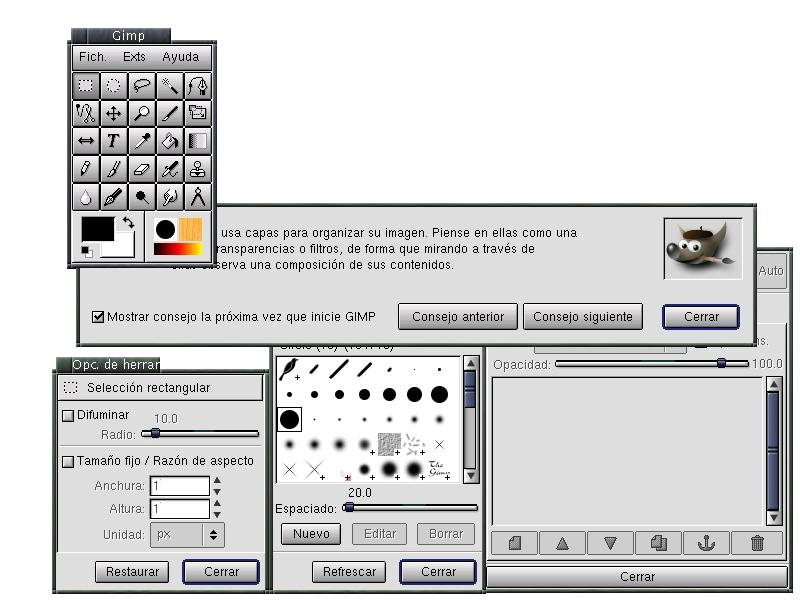
\includegraphics[width=0.88\textwidth]{imagenes/gimp.eps}
\caption{Aspecto de The GIMP al usarlo por primera vez}
\end{figure}

\subsection{Los diferentes formatos de im�gens}

Del  formato  del  fichero  que utilices  para  guardar  tus  im�genes
depender�  la calidad  de  las  mismas (las  fotos  almacenadas en  un
formato que permita bastante compresi�n normalmente lo hace a costa de
su calidad)  y el espacio  que ocupe. Algunos adem�s  pueden almacenar
informaci�n relativa al  tama�o de la foto para la  impresi�n (TIFF) e
informaci�n sobre su transparencia (GIF, PNG).

Existen muchos tipos de formato, cada uno para su uso.
The GIMP tiene soporte para estos:

\begin{itemize}

\item  BMP: desarrollado  e impulsado  por Microsoft,  propietario del
mismo.  BMP es  una abreviatura  de Windows  BitMaP (Mapa  de Bits  de
Windows).

\item  CEL: este  formato es  originario del  Animator Studio.  Es muy
utilizado para guardar {\em sprites},  o mejor dicho im�genes peque�as
para juegos.

\item FITS: es el formato standard en Astronom�a.

\item FLI: el formato FLI fue originalmete creado por Autodesk para 
la realizacion de animacines virtuales con ordenador.

\item Fax G3: este formato se usa para poder procesar faxes.

\item GBR: es el formato para las Brochas de GIMP (Gimp brush). 

\item GIF: El  Formato de Intercambio de Gr�ficos  (GIF) fue inventado
por CompuServe  y es uno est�ndares  de las im�genes en  la World Wide
Web. Sin embargo, las patentes de Unisys e IBM que cubren el algoritmo
de compresi�n LZW que es utilizado  para crear los archivos GIF, hacen
imposible tener software libre que genere GIFs adecuados.

\item  GIH: este  formato  lo usa  The GIMP  para  guardar las  brochas
animadas que  aparecen en  las herramientas. GIH  es el  acr�ninimo de
(GIMP Image Hose).

\item GIcon:  este es el formato  nativo de los iconos  dThe GIMP. Este
formato s�lo permite escala de grises.

\item HRZ: formato siempre a 256x240  pixels y es (o mejor, era) usado
para edici�n de im�genes de TV. No tiene compresi�n.

\item Jpeg:  es acr�nimo  de Joint  Photographic Experts  Group (Uni�n
de  Grupo  de  Expertos  en  Fotograf�a)  y  funciona  con  todas  las
profundidades de color. La compresi�n  de la imagen es ajustable, pero
altas compresiones da�ar�n la calidad final  de la foto, ya que es una
compresi�n con p�rdidas.

\item  MPEG:  acr�nimo  de  Motion Picture  Experts  Group  (Grupo  de
Expertos  en  Animaci�n). Es  un  bien  conocido  de los  formatos  de
animaci�n.

\item PAT: es el formato nativo de Patrones (Patterns) dThe GIMP.

\item PCX: este formato gr�fico fue  creado por ZSoft y difundido por 
la familia de programas de dibujo Paintbrush.                         

\item PIX: este es el formato usado por el programa Alias/Wavefront en
estaciones SGI  (Silicon Graphics). S�lo  permite im�genes a  color de
24-bits e im�genes en escala de grises de 8-bits.

\item PNG:  El formato PNG  (Portable Network Graphics) es  un formato
gr�fico que usa compresi�n sin  p�rdidas (loseless compression). Es el
formato actualmente  recomendado por  la organizaci�n W3C  (World Wide
Web Consortium) para im�genes sin p�rdida de calidad.

\item PNM: Acr�nimo de Portable  aNyMap. PNM permite paleta de colores
indexada, escala de grises e im�genes a todo color.

\item PSD:  formato usado por  el Adobe Photoshop (The  GIMP mantendr�
las capas existentes).

\item PSP: formato usado por el  PaintShop Pro (The GIMP mantendr� las
capas existentes).

\item PostScript (PS): PostScript fue creado por Adobe. Es un lenguaje
para describir  p�ginas, y  es usado  principalmente por  impresoras y
otros dispositivos de impresi�n. Es una manera estupenda de distribuir
documentos.  Tambi�n  podemos leer  ficheros  PDF  (Acrobat) con  esta
opci�n.

\item  SGI: es  el formato  originalmente usado  por las  aplicaciones
gr�ficas de SGI.

\item  SUNRAS:  acr�nimo de  SUN  RASterfile.  Este formato  es  usado
principalmente por las diferentes  aplicaciones de Sun. Permite escala
de grises, color indexado y todo color.

\item TGA:  este formato permite  compresi�n a 8,  16, 24, 32  bits de
profundidad.

\item TIFF:  acr�nimo de  Tagged Image File  Format. Este  formato fu�
dise�ado para ser un estandar. Este es un formato de alta calidad y es
perfecto  cuando quieras  importar  im�genes de  otros programas  como
FrameWork o Corel Draw.

\item  URL:  acr�nimo  de  Uniform Resource  Locator  (Localizador  de
Recursos  Uniforme).  Podr�s  descargar   una  im�gen  desde  internet
dir�ctamente  al GIMP.  El  formato  del nombre  del  fichero es  {\tt
ftp://direcci�n/archivo} o {\tt http://direcci�n/archivo}.

\item WMF: acr�nimo de Windows Meta File (Meta Fichero de Windows). Es
un  formato que  permite guardar  tanto gr�ficos  vectoriales como  en
mapas de bits.

\end{itemize}


% Para aprender  a manejar GIMP s�lo  se necesitan ganas, osad�a  y unos
% cuantos ratitos para sentarse y  ponerse a jugar con las herramientas,
% filtros  y  scripts  que  proporciona.  Si  quieres  sacarle  el  jugo
% puede  resultarte muy  �til  alg�n  libro sobre  {\sf  The GIMP}  como
% \cite{gimpref}.


%\section{DIA}

\section{QCad}

\index{QCad}

{\sf  QCad}  es un  programa  de  dise�o  asistido por  ordenador  (en
ingl�s  CAD,  de  Computer  Aided Design)  para  trabajar  con  planos
bidimensionales.  No necesitas  conocimientos  de CAD  para empezar  a
trabajar  con {\sf  QCad}, sobretodo  si  ya has  trabajado con  otros
programas de CAD. {\sf QCad} es realmente f�cil de utilizar si prestas
atenci�n a la barra de estado de la parte inferior.

La siguiente  figura muestra {\sf  QCad} con  uno de los  ejemplos que
incluye,  el dise�o  de  un tornillo  de banco.  Como  puedes ver,  la
prioridad en un plano no es la estetica sino la precisi�n.

Mira el ap�ndice de la p�gina \pageref{recursos} para ver la direcci�n
de un tutorial para {\sf QCad}

\begin{figure}[hbtp]
\centering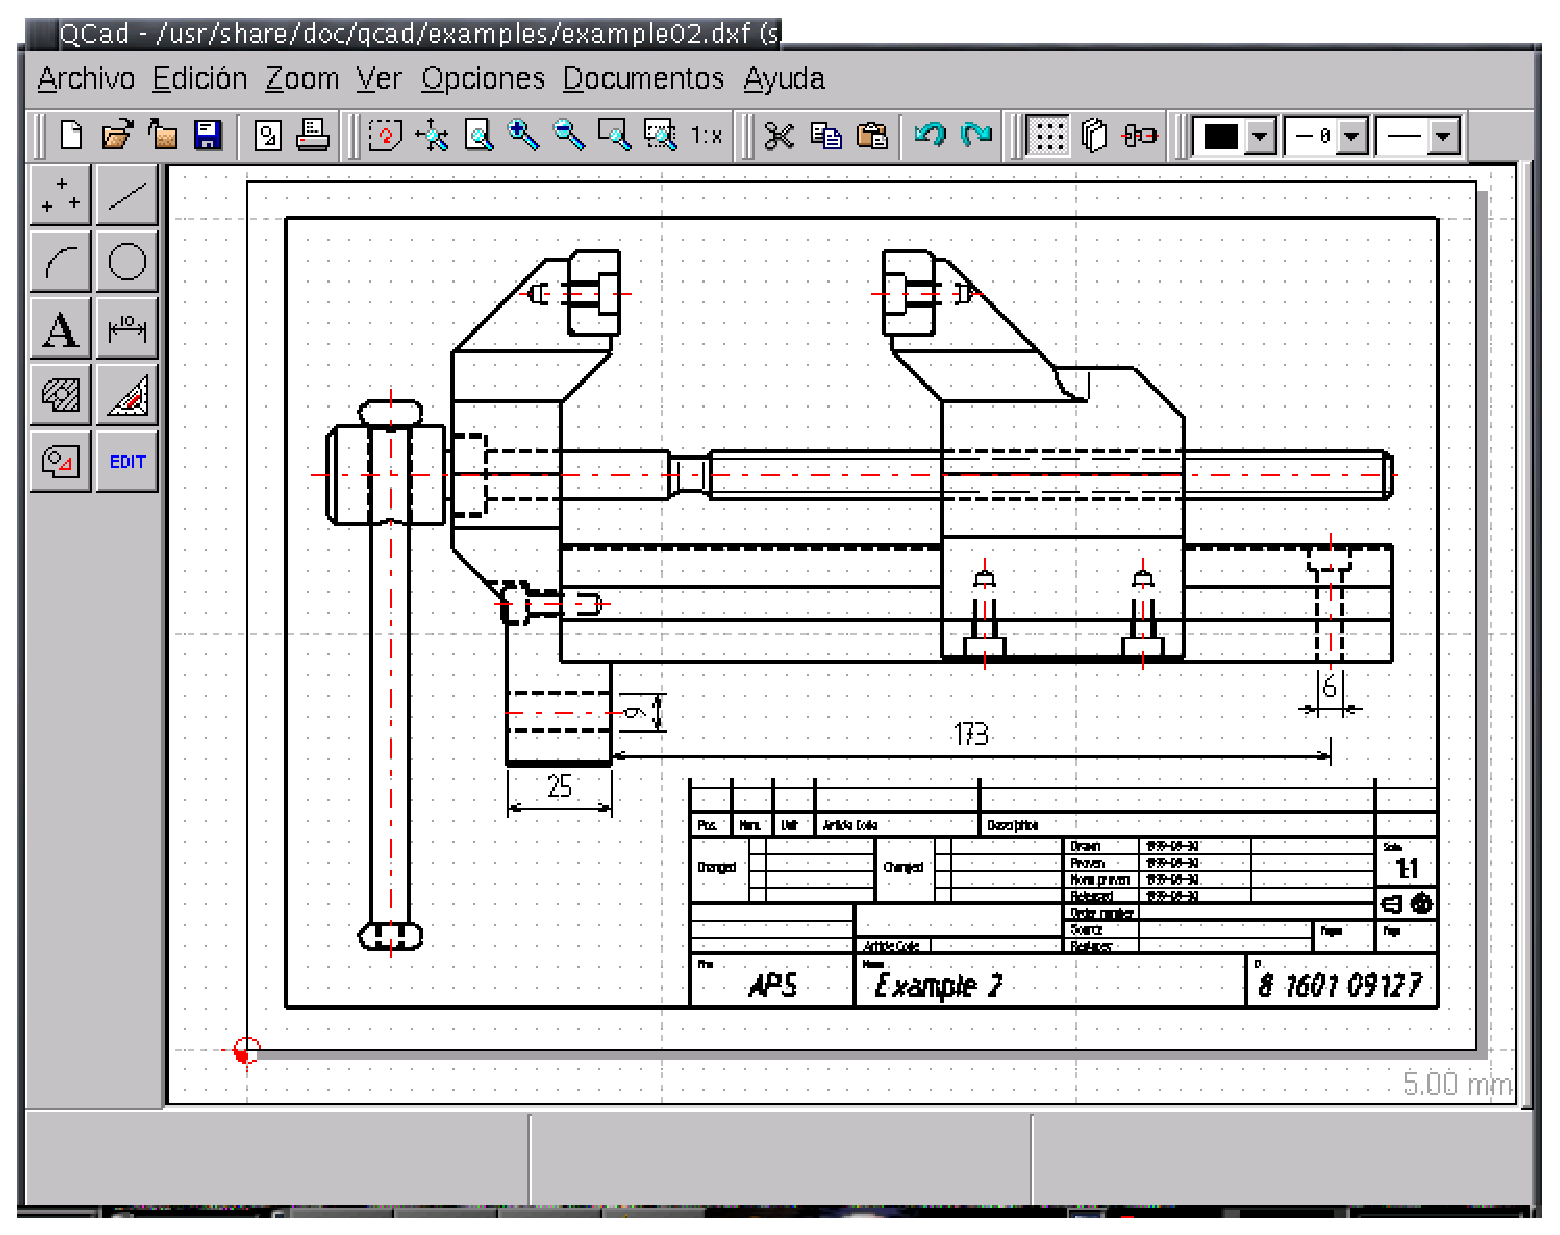
\includegraphics[width=0.4\textwidth]{imagenes/qcad_main.eps}
\caption{QCad con un dise�o de ejemplo}
\end{figure}


%Autor: Sirma,darkside

\chapter{OpenOffice}


%%%%%%%%%%%%%%%%%%%%%%%%%
% Secci�n: Introducci�n %
%%%%%%%%%%%%%%%%%%%%%%%%%
\section{Introducci�n}

OpenOffice.org es un entorno de oficina que contiene todas las
herramientas para desenvolverse en un ambiente de trabajo, as� como
tambi�n hogare�o. 
Este set de herramientas tiene sus raices en StarOffice, 
un suite de oficina que desde mediados de los ochenta se desarrollaba en Alemania,
a cargo de una compa��a llamada StarDivision,  cuyos derechos fueron comprados en  
1999 por Sun Microsystems.
La version 5.2 of StarOffice se lanz� en junio del 2000, y la versi�n 6.0 sali�
en mayo del 2002. Lo m�s extraordinario del desarrollo de StarOffice 6.0 es que se
desarrolla mayoritariamente en el contexto del proyecto Open Source de OpenOffice.org. 
A efectos de posibilitar dicho desarrollo, Sun hizo p�blico el c�digo fuente de la mayor�a 
de los m�dulos de StarOffice (excepto por algunos m�dulos de proveedores externos, que no 
han entrado en el proyecto), y estableci� el proyecto OpenOffice.org. Esto no significa sin 
embargo que Sun deja en manos de voluntarios el desarrollo futuro del suite: la mayor�a del
trabajo todav�a se lleva a cabo por desarrolladores de Sun. Sun tambi�n se encarga de los 
costes operacionales del proyecto OpenOffice.org.

OpenOffice.org es uno de los grandes competidores del paquete de oficina
\emph{Microsoft Office}, ya que el OpenOffice.org es compatible con los
formatos de archivos del MS-Office, adem�s que existen versiones para
GNU/Linux, MS-Windows, y otros sistemas operativos; y por �ltimo, una
caracter�stica muy importante: es gratis.

Openoffice.org es una suite ofim�tica que est� compuesta por diferentes m�dulos
que se pueden cargar de forma independiente.
Este cap�tulo no est� orientado a ser un manual exhaustivo de
OpenOffice.org, sino m�s bien una introducci�n a este enorme paquete,
donde se explicar� el funcionamiento b�sico de los m�dulos mas
importantes y se mencionar� la existencia de los dem�s m�dulos.


%%%%%%%%%%%%%%%%%%%%%%%%%%%%%%%%%%
% Secci�n: OpenOffice.org Writer %
%%%%%%%%%%%%%%%%%%%%%%%%%%%%%%%%%%

% Caracter�sticas generales:
%				Autocorrecci�n
%				Impresi�n
%				Lectura de archivos Word
%
% Caracteristicas mas avanzadas:
%				DirectCursor
%				Autotexto

\section{OpenOffice.org Writer: Procesador de textos}


\subsection{Introducci�n:}

OpenOffice.org Writer es un procesador de textos\footnote{%
Un procesador de textos es un programa con el que se generan diferentes documentos
de texto como, cartas, informes o incluso el presente libro
} avanzado, con el que se pueden crear diferentes tipos de documentos en los
que se pueden insertar tablas, esquemas, gr�ficos, etc. Tambien cuenta con plantillas \footnote{%
Una plantilla es el esqueleto de un modelo de documento en el que vamos insertando
nuestro texto, esto se explica en el apartado \ref{Uso de Plantillas} 
} que simplifican la creaci�n de: cartas, folletos, art�culos, informes, curriculum
vitae, libros, etc. Adem�s de las anteriores existen multitud de utilidades
que facilitan el uso del procesador, como son el autocorrector, el autoformato,
etc.

Un punto muy importante a favor de OpenOffice.org Writer es la compatibilidad con los documentos
guardados con formatos propietarios como Microsoft Word, no obstante siempre
se podr�n exportar documentos de cualquier procesador de texto guardandolo en
formato de texto Enriquecido (RTF\footnote{%
RTF: formato de texto enriquecido, es un formato estandar que puede ser entendido
por la practica totalidad de editores de texto.
}). OpenOffice.org Writer posee un sisema de ayuda que puede ser consultado de forma contextual
(pulsando \boton{F1}) mientras se edita el documento o buscando en los temas de ayuda.
Se debe tener en cuenta que se puede acceder a todas las funcionalidades del
editor a trav�s de los diferentes men�s con el rat�n como con diferentes combinaciones
de teclas, denominadas teclas r�pidas, que permitir�n realizar cualquier tarea
de una forma mucho m�s r�pida y eficaz.

\subsection{Como empezar:}

Este es el aspecto que tiene la pantalla del OpenOffice.org Writer, antes de comenzar a crear
nuestro documento vamos a determinar para que sirven los principales men�s que
encontramos en la aplicaci�n.

%\figura{OpenOffice.org Writer}{principal_p.eps}


\subsubsection{Especificaciones del men� principal:}

%IMAGEN DE LA BARRA SUPERIOR

\begin{description}
\item [\textmd{Archivo:}]Este men� se utiliza para abrir, cerrar, imprimir o crear
asistentes para documentos, para cerrar OpenOffice.org Writer hay pulsar en este men� la
opci�n cerrar.
\item [\textmd{Editar:}]Sirve para modificar el texto, cortar, pegar, seleccionar,
buscar y remplazar, etc.
\item [\textmd{Ver:}]Es posible ver el documento a distinta escala, tener acesso directo
a los archivos del usuario a traves del beamer, ver la regla, la barra de estado,
los submen�s de las barras de herramientas.
\item [\textmd{Insertar:}]Con este men� se insertan campos, simbolos, encabezados,
indices, notas, referencias, tablas, imagenes, objetos.
\item [\textmd{Formato:}]Modificaci�n de los parrafos, caracteres, p�ginas, el estilo
y aplicaci�n del autoformato.
\item [\textmd{Herramientas:}]Aqu� se encuentra el diccionario de sinonimos, la ortografia,
la numeraci�n de capitulos y p�ginas, actualizar el documento y las macros\footnote{%
Una macro es una utilidad que creamos para automatizar tareas repetitivas.
}.
\item [\textmd{Ventana:}]Sirve para ir de una ventana a otra, es decir cuando se tiene
abierto m�s de un documento se tiene la posilididad de desplazarse de uno a
otro, verlos en cascada, azulejearlos que es verlos todos a la vez en la pantalla,
ver dos documentos en horizontal o en vertical, cerrar todas la ventanas a la
vez y ver cuantos documentos se tienen abiertos.
\item [\textmd{Ayuda:}]Para obtener ayuda sobre el contenido o sea sobre OpenOffice.org Writer,
tener el asistente abierto mientras escribimos, o la ayuda activa que al posicionar
el cursor sobre un icono da una explicaci�n de para que se utiliza (est� sin
traducir al castellano).
\end{description}

\subsection{Uso de la ayuda: }


\subsection{El documento:}

Una vez que se ha abierto OpenOffice.org, para abrir una sesi�n de OpenOffice.org Writer hay
que abrir un documento ya sea nuevo o existente.


\subsubsection{Como crear un nuevo documento:}

Para crear un documento nuevo simplemente se hace doble click sobre el icono
Nuevo Texto y aparecer� el nuevo documento. Tambien se puede abrir un nuevo
documento seleccionando en el men� \menu{Archivo} la opci�n \menu{Nuevo} y elegir
\menu{Texto} .


\subsubsection{Como abrir un documento existente:}

Con OpenOffice.org Writer existe la posibilidad de trabajar con documentos de formatos
muy diferentes, como pueden ser los documentos de Microsoft Word, html, TXT,
RTF, Winword, etc. Para abrir un documento existente se pulsa en \menu{Archivo}
y se elige \menu{Abrir} y aparecer� un cuadro de dialogo en el que aparece la
ubicaci�n de los archivos en nuestro ordenador, se elige la ruta correcta y
el nombre del archivo y se pulsa abrir o utilizamos las teclas r�pidas \boton{Ctrl-O}.

%Figura 5.3.2.: Abrir documento existente


\subsubsection{Guardar, guardar como:}

La primera vez que se guarda un documento hay que darle un nombre y decidir
su ubicaci�n (donde se quiere guardar). Guardar como, se utiliza para guardar
el documento con un nombre de archivo, por ejemplo: Manual.doc, y en una localizaci�n
determinada en el sistema de archivos, por ejemplo: \comando{/home/usuario/OpenOffice.org Writer/personal/trabajos/Manual.doc},
para Guardar Como se pulsa sobre \menu{Archivo} y despu�s sobre \menu{Guardar como},
y se elige la ruta y el nombre del archivo en el cuadro de dialogo.

Guardar, se utiliza para conservar los cambios que se realizan en el documento
mientras se escribe, para guardar se pulsa sobre \menu{Archivo} y despu�s sobre
\menu{Guardar} y todos los cambios ser�n guardados.

%Figura 5.3.3.: Guardar como.


\subsubsection{Edici�n y formateado de un documento:}

Como se ha comentado anteriormente el texto puede formatearse mientras se escribe
o una vez que se ha terminado la edici�n del documento. Si se quiere formatear
el texto mientras se escribe se activa la orden, por ejemplo activar \boton{negritas},
y una vez acabado se desactiva la opci�n. Para formatearlo una vez que terminado
hay que seleccionar el texto o la parte del texto que queramos modificar, para
se�alarlo basta con colocar el puntero del rat�n al comienzo del texto y pulsando
el bot�n derecho arrastrar el rat�n hasta el final de la selecci�n, tambien
se puede seleccionar mediante los cursores manteniendo la tecla de mayusculas
pulsada.

Para ver el documento en una escala mayor o menor se utiliza....Para cambiar
el tama�o y tipo de letra (una vez seleccionada) se pulsa \boton{Formato}......y
aparecer� un cuadro de dialogo en el que se puede elegir el tama�o de la letra,
el tipo de fuente, Negrita, cursiva, etc. Una vez seleccionados los cambios
pulsamos \boton{Aceptar} y se modificar� el texto seleccionado. Para ver las marcas
del texto de principio o fin de p�rrafo, tabulaciones, sangr�as, etc., se pulsa
en \menu{Ver} y despu�s se selecciona ......... (Caracteres no Imprimibles)


\subsubsection{Trabajar con tablas:}

Para insertar una tabla en un documento se selecciona \menu{insertar} y se pulsa
\menu{tabla}, aparecer� un cuadro de di�logo.... 

Para modificar el aspecto de la tabla en el documento se selecciona \menu{Formato},
\menu{Tabla} y en el cuadro de di�logo se pulsa en la pesta�a Tabla.......

%Figura 5.3.4.: Vista Previa.

Para cambiar el ancho de las columnas..... Para cambiar los bordes..... El grosor
o estilo de las l�neas.....color..... sombras.......Como introducir texto en
las casillas.........., formato del texto de la tabla ......


\subsubsection{Imprimir un documento:}

Para poder imprimir correctamente un documento se debe tener previamente configurada
la impresora que se vaya a utilizar\footnote{%
La impresora se configura siendo Administrador y desde el escritorio de OpenOffice.org
(Desktop)
}. Antes de imprimir el documento es conveniente que veamos el aspecto que va
ha tener una vez impreso, para previsualizarlo se pulsa en \menu{Archivo} y despu�s
en \menu{Vista preliminar}, en la pantalla aparece una barra de herramientas
donde existen una serie de botones con los que podremos por ejemplo ampliar
el documento, mostrar varias p�ginas en pantalla, etc. Para ver el documento
se puede pulsar el icono con forma de prism�ticos.

%Figura 5.3.4.: Vista Previa.

Una vez visualizado el documento, para imprimir se selecciona \menu{Archivo}
y despu�s \menu{Imprimir}, se puede pulsar el icono de la impresora, abriendose
un cuadro de dialogo en el que se puede ver una serie de opciones de impresi�n,
impresora, propiedades de la impresora, donde elegiremos el formato del papel,
la orientaci�n, el area de impresi�n, el n�mero de copias, etc. Tambi�n se
puede utilizar la serie de teclas \boton{Ctrl-P}

%Figura 5.3.5.: Cuadro de Dialogo de Impresi�n.


\subsection{\label{Uso de Plantillas}Uso de plantillas:}

%Figura 5.3.6.: Plantillas.


\subsection{Teclas rapidas:}


\subsection{Salir de OpenOffice.org Writer:}

Para salir de OpenOffice.org Writer, se pulsa \boton{Archivo} y se elige \boton{Salir}, pudiendose
utilizar tambi�n las teclas r�pidas \boton{Ctrl-Q}. Si el documento no se ha guardado
previamente aparecer� un cuadro de dialogo
 que preguntando si se quieren guardarlos cambios realizados en el documento, seleccionando \boton{Si} los cambios ser�n
almacenados y se cerrara la aplicaci�n, si por el contrario elegimos \boton{No}
los cambios no son guardados y se perder� todas las modificaciones realizadas
en el documento, finalmente si se pulsa \boton{Cancelar} se retornar� al documento.

%Figura 5.3.6.: Salir de OpenOffice.org Writer.

%Figura 5.3.7.: Cuadro de Dialogo para Salir
% \end{document}
%%%%%%%%%%%%%%%%%%%%%
% Secci�n: StarCalc %
%%%%%%%%%%%%%%%%%%%%%


\section{StarCalc: Hoja de C�lculo}

% La verdad que no s� que meter ac� :-(

%Carlos P�rez P�rez {\\tt cperezperez@terra.es}

%*****************************************************
%                           Introducci�n             *
%*****************************************************

\subsection{Introducci�n}

Una hoja de c�lculo\footnote{Tambi�n denominada Planilla de C�lculo} es una
herramienta puesta al alcance del usuario para solucionar una cierta clase
de problemas. Estos problemas van desde llevar el c�lculo de la contabilidad
del hogar hasta el �nalisis de datos estad�sticos pasando por un sinf�n de
posibilidades.
El uso de una hoja de c�lculo queda supeditada a lo que el usuario quiera,
pero, hay situaciones en las que se hace imprescindible el uso de una hoja de
c�lculo. Desde llevar la contabilidad de peque�as empresas, en las que se
requieran sumar grandes cantidades de cifras que la hoja de c�lculo puede
hacer autom�ticamente, utilizarlo para hacer regresiones estad�sticas no
excesivamente complejas, llevar el control de pedidos, de ventas, de \ldots{}.
Un largo etc�tera cuyo principal punto en com�n es el de evitar c�lculos
manuales tediosos que puedan inducir a errores.
Definido el problema al que se puede enfrentar el usuario ahora queda la
elecci�n del programa de hoja de c�lculo. En el mercado hay una gran cantidad
de paquetes que incorporan hojas de c�lculo. Aqu� se expondr� el uso de la
StarCalc, la hoja de c�lculo perteneciente al paquete ofim�tico OpenOffice.org.
Pero lo aqu� explicado puede ser aplicado sin esfuerzo al uso de otras hojas
de c�lculo, como la Excel.
El lector debe tener en cuenta que aqu� no se explican todas las opciones  y
caracter�sticas que incorpora StaCalc, s�lo se trata de una introducci�n  al
uso de la misma as� como una serie de pr�cticas en las que se tratar� de
extender la parte te�rica.

%**********************************************************
%                    Primeros Pasos                       *
%**********************************************************

\subsection{Primeros Pasos}

\subsubsection{Entorno de trabajo.}

El entorno de trabajo de la StarCalc se hace familiar para aquel
usuario que conozca el uso de las hojas de c�lculo. Es un entorno
totalmente gr�fico e intuitivo desde el principio. En el que podemos
observar una barra de men�s donde se encuentran las operaciones que se
pueden hacer con la StarCalc. Debajo se hallan una serie de botones
que se usan para acceder m�s r�pida y c�modamente a funciones y
acciones que se encuentran en los men�s.\\

%<Gr�fico principal>
\figura{La hoja de c�lculo StarCalc}{StarCalc}

La zona de men�s, all� se posicionan el men� \menu{Archivo},
\menu{Editar}, \menu{Ver}, \menu{Insertar}, \menu{Formato},
\menu{Herramientas}, \menu{Datos}, \menu{Ventana} y \menu{Ayuda}.
Dentro decada una  de ellas se agrupan las diferentes macros que la StarCalc
tiene predefinidas y que nos permiten realizar las tareas propias
de la hoja de c�lculo. Ver figura \ref{fig:StarCalcMenus}.

%<Gr�fico menu>
%\figura{Los men�s de la StarCalc}{StarCalcMenus}

La siguiente zona est� conformada por una serie de botones que permiten el
acceso  r�pido a funciones definidas. Este �rea tambi�n se extiende a la parte
izquierda de  la pantalla, que pueden verse en las figuras
\ref{fig:StarCalcBotones} y \ref{fig:StarCalcBotoensLaterales}.

%<Gr�fico botones>
\figura{Barra de botones superiores}{StarCalcBotones}
\figura{Barra de botones laterales}{StarCalcBotonesLaterales}

Luego se nos presenta la zona de trabajo, esto es, la parte destinada a la
introducci�n,  modificaci�n, c�lculo y presentaci�n de datos, que puede
observarse en la figura \ref{fig:StarCalcTrabajo}.
 
%<Gr�fico trabajo> 
\figura{Zona de trabajo}{StarCalcTrabajo}

La �ltima zona est� conformada por una l�nea en la que se presentan una serie
de datos  sobre caracter�sticas generales de la hoja en la que estemos
trabajando.   

%<Gr�fico parte baja>
%\figura{L�nea inferior}{StarCalcLinea}

%*************************************************************
%                   Creaci�n de Nuevas Hojas                 *
%*************************************************************

\subsubsection{Creaci�n de nuevas hojas}
Para crear una nueva hoja se puede recurrir a varias formas de hacerlo.
Por un lado se puede hacer doble click en el icono de
\comando{Nueva Hoja de C�lculo} dentro del escritorio del entorno OpenOffice.org.
Tambi�n se puede crear en el men� \comando{Archivo}, submen� \comando{Nuevo},
y elegir \comando{Hoja de c�lculo}. Otra forma es utilizar las plantillas,
para ello se puede acceder al men�  \menu{Archivo}, submen� \menu{Nuevo},
y \menu{Plantillas}, o tambi�n presionar \boton{Ctrl+N}.

%Moverse por la hoja de C�lculo.
\emph{Selecci�n de celda.}
Las celdas dentro de la hoja se pueden seleccionar bien usando el rat�n 
o con el teclado. Con el rat�n se presiona en la celda de inicio y, sin 
soltar, se extiende la selecci�n moviendo el rat�n hasta llegar a la celda 
final que se quiere seleccionar. Con el teclado, se posiciona con las teclas 
de direcci�n sobre la celda a seleccionar y se presiona la teclas \boton{May�sculas}. 
Sin soltar dicha tecla se seleccionan las celdas deseadas con las teclas de 
direcci�n.\\ 
Para seleccionar celdas que no sean contiguas se utilizar� el rat�n y la 
tecla \boton{Control}. Se selecciona el primer rango de celdas o una sola, y a 
continuaci�n se seleccionan las celdas o rangos deseados sin soltar la  
tecla \boton{Control}.
Para el caso en el que la selecci�n de celdas quede fuera de las ventanas, 
hay que hacer notar que el movimiento es autom�tico y no se necesita 
preocuparse hasta d�nde llegar. 
Las columnas y filas se pueden selccionar enteras si se presiona sobre 
el r�tulo de fila o columna. 

\subsubsection{Abrir hoja desde archivo} 
%Las maneras de recuperar el trabajo (de otro o nuestro). 
Para recuperar un trabajo desde el lugar donde est� almacenado acudiremos
al men� \menu{Archivo} y \menu{Abrir} con lo que aparecer� el cuadro de
opciones para recuperar el archivo, como se aprecia en la figura
\ref{fig:StarCalcAbrir}.

\figura{Recuperar archivo}{StarCalcAbrir}

Se puede acceder al cuadro de di�logo de abrir archivo presionando
\boton{Ctrl+O}.

%*****************************************************************
%                   Introducci�n de datos                        *
%*****************************************************************

\subsubsection{Introducci�n de datos.} 
 
%Manera adecuada de poner los datos en las celdas :) 
 
Se aceptan dos grandes tipos: constantes y f�rmulas. 
Las constantes se dividen en: valores num�ricos, de texto y de fecha y hora.
Para los valores num�ricos y de texto se aceptan: 
N�meros del 0 al 9 y ciertos car�cteres especiales, tales como +-E e () . , 
\$ \% y /. Las restantes entradas se considerar�n de texto. Si se quiere 
utilizar un valor num�rico como texto se antepondr� el signo ' y luego se 
introduce el valor. 

Para introducir datos nos situaremos en la celda adecuada presionando 
en ella y escribiremos aquello que queramos. 
 
StarCalc puede ayudarnos a introducir datos, por ejemplo, en series de 
n�meros podemos poner el primer n�mero y seleccionar la celda. En la parte
inferior derecha hay un punto negro, al seleccionarlo el puntero del rat�n se 
convierte en una cruz, arrastr�ndolo hacia donde queramos poner los datos se
extender� la selecci�n y la StarCalc sumar� autom�ticamente los siguientes datos.
En el caso de que los n�mero no sean correlativos se pueden poner los dos
primeros n�meros de la serie y la StarCalc har� el resto. 

Se puede hacer lo mismo con los nombres de los meses, si se introduce enero, y
siguiendo el procedimiento anterior se conseguir� que vaya escribiendo todos
los meses. 
La StarCalc muestra un r�tulo al lado del puntero del rat�n, de esta manera
sabremos hasta d�nde llegar sin tener que hacer c�lculos mentales.

\emph{Protecci�n de datos.} Se pueden proteger libros enteros u hojas
individuales, de manera que  se permita acceso de s�lo lectura o sin acceso. A
trav�s del men�  \menu{Herramientas} y \menu{Proteger}. 
Tambi�n se pueden proteger y desproteger celdas individuales. 
 
%*************************************************************************
%                            Construcci�n de F�rmulas                    *
%*************************************************************************

\subsubsection{Construcci�n de f�rmulas.}
 
Creaci�n de f�rmulas para la transformaci�n de los datos.\\ 
 
Se selecciona una celda vac�a y se introduce el signo igual precedido de 
la expresi�n aritm�tica a utilizar. Por ejemplo, para sumar 3 y 6 pondremos:\\ 
\[=3+6\]
 
\emph{Precedencia de los operadores:}
\begin{itemize} 
\item Se procesan primero las expresiones entre par�ntesis. 
\item Se ejecutan la multiplicaci�n y la divisi�n antes de la suma y la resta. 
\item Los operadores del mismo nivel se calculan de izquierda a derecha. 
\end{itemize}

\emph{Los par�ntesis.} 
Hay que incluir un par�ntesis cerrado por cada uno que
se abra.\\
\emph{Referencias a las celdas.}
Dentro de una f�rmula nos podemos referir a una celda de diferentes maneras. 
Escribiendo A1 haremos referencia a la celda de la fila 1 columna A, que
tambi�n puede ser seleccionada con el rat�n. 
En este punto hay que diferenciar el tipo de referencia que se va a utilizar.\\ 
\emph{Referencias relativas.}
Se refieren a las celdas por sus posiciones en relacci�n a la celda que
contiene la f�rmula. De esta manera la celda A1 se convertir� en B2 si
la f�rmula se mueve una fila hacia debajo y una columna hacia la derecha.\\ 
\emph{Referencias absolutas.} 
Se identifica a la celda por su posici�n fija, la f�rmula har� referencia 
siempre a la misma celda aunque se mueva la f�rmula. La manera de hacer esto 
es utilizando el signo \$. Esto es, \$A\$1 hace referencia a la fila 1
columna A  en todo momento. A\$1 har� referncia a la fila 1 simpre y a la
columna se calcular�  de forma relativa a la f�rmula. El caso contrario
ser�a \$A que mantendr�a fija  la columna.  N�tese que se puede hacer
referencia a cualquier celda dentro del libro de  trabajo.\\
 
%<Ver si se puede en otros libros>. 

\emph{Uso de funciones.}
Las funciones tal y como las hemos visto pude que no tengan demasiado sentido 
si se trata, por ejemplo, de sumar una gran cantidad de celdas:\\
\[=A1+A2+A3+A4+A5+A6+A7+A8+A9+A10+A11+A12\]
por eso se puede utilizar la sintaxis que provee la StarCalc\\
\[=SUMA(A1:A12)\]
 
Se puede utilizar cualquier funci�n definida dentro de la StarCalc pas�ndole
los par�metros adecuados. Sin embargo, no se pueden conocer o retener todas 
las funciones que tiene la hoja, por eso se puede utilizar insertar funci�n 
que presentar� un cuadro con las distintas funciones existentes, una peque�a 
explicaci�n y los par�metros que se necesitan. 

%****************************************************************
%                        Formateo de la Hoja                    *
%****************************************************************

\subsubsection{Formateo de la hoja.} 
%Utilizaci�n de los formatos de datos correctos y adecuados.
Para poner el formato correcto de los datos podemos seleccionar
las celdas a formatear y acudir al men� \menu{Formato} \menu{Celda...}
y se nos presentar� un cuadro con las diferentes opciones a
configurar, desde el tipo de cuadro hasta el idioma, la fuente, el
color, la justificaci�n o la orientaci�n de la escritura. Al finalizar
la configuraci�n presionamos \boton{Aceptar}.

%****************************************************************
%                     Impresi�n y Presentaci�n			*
%****************************************************************

\subsubsection{Impresi�n y presentaci�n.}
%Imprimir documentos y presentaci�n en pantalla
%(eso de los colores y las l�neas).
El uso de la impresi�n dentro de la StarCalc sigue el mismo esquema que en el
resto de la suite OpenOffice.org. Seleccionaremos el men� \menu{Archivo} e
\menu{Imprimir}, tambi�n podemos presionar las teclas \boton{Ctrl+P}. En
ambos casos se mostrar� un cuadro de di�logo. En el caso de que no necesitemos
ajustar las propiedades presionaremos \boton{Aceptar} y StarCalc mandar� el
trabajo a la cola de impresi�n.
 
%****************************************************************
%                        Salvando nuestro esfuerzo              *
%****************************************************************

\subsubsection{Salvando nuestro esfuerzo.} 
%Formas de grabar en un archivo lo que hayamos hecho. 
Para guardar los datos con los que estamos trabajando acudiremos a
\menu{Archivo} y \menu{Guardar} o \menu{Guardar como} si
queremos guardarlo bajo otro nombre. En el caso de que el archivo
sea nuevo se nos presentar� el di�logo de guardar como para indicar
a la StarCalc bajo que nombre y tipo de archivo deseamos que sea
salvado nuestro trabajo.

%***************************************************************
%                     An�lisis de Datos                        *
%***************************************************************

\subsection{An�lisis de Datos}
%An�lisis de datos. 
%Funciones Comunes. 
 
\subsubsection{Funciones comunes.} 
%Las funciones que ofrece la StarCalc 
Sintaxis de las funciones: Las funciones presentas dos partes
diferenciadas, por un lado, el nombre de la funci�n, por el otro, sus
argumentos. Los argumentos de una funci�n deben estar entre par�ntesis
inmediatamente despu�s del nombre de la funci�n y su cantidad
depender� del tipo de funci�n que se use. Tambi�n hay que destacar el
hecho que dentro de los argumentos se pueden incluir tanto otras
funciones, con sus propios argumentos, como valores num�ricos, valores
de texto o valores l�gicos, as� como matrices y valores de error. La
forma m�s sencilla de insertar funciones es us�ndo el autopiloto de
funciones que se encuentra en el men� \menu{Insertar}, \menu{Funci�n},
o presionando las teclas \boton{Ctrl+F2} o usando el bot�n que se
encuentra en las barras de botones, d�nde se introducen las f�rmulas.
Aqu� no se van a exponer todas las funciones que existen e la
StarCalc, para ver todas las funciones que la hoja puede ofrecer puede
consultar el Autopiloto de Funciones, all� las encontrar� agrupadas
seg�n el uso que se les quiera dar. Ver figura \ref{fig:StarCalcFucniones}.

\figura{Autopiloto de funciones.}{StarCalcFunciones}

\subsubsection{Fechas y horas.} 
%Manipulaci�n de fechas para presentaci�n y utilizaci�n en c�lculos. 
Las fechas se introducen directamente en las celdas siguiendo alguno
de los siguientes formatos que son perfectamente legibles por
StarCalc: d/mm/aa; d-mmm-aa, d--mmm o mmm-aa. Para conseguir 5 de
Noviembre el a�o 2000, teclearemos \comando{5-nov-2000} y se nos
mostrar� tal cual la hemos introducido. En aquellos formatos en los
que se omita alguna parte de la fecha se tratar�n de distinta manera,
as� si falta el d�a se introduce autom�ticamente el d�a primero, si es
el a�o se introduce el a�o en curso.  N�tese que no puede faltar el
mes en los formatos presentados. Para introducir series de fechas
utilizaremos lo aprendido en la secci�n de introducci�n de datos, esto
es, podemos extender la selecci�n autom�ticamente con el rat�n.  Para
la introducci�n de horas se pueden seguir los siguientes formatos:
h:mm AM/PM; h:mm;ss AM/PM; h:mm; h:mm:ss; mm:ss.0; [h]:mm:ss. El
lector interesado puede mirar el Autopiloto de funciones donde se
encuentran algunas funciones para utilizar y transformar fechas.
 
\subsubsection{An�lisis financiero.} 
%C�lculo de TAE, VAN, TIR, rentabilidades, intereses, etc. 
En una hoja de c�lculo no pod�an faltar las funciones referidas a
operaciones financieras, tales como el valor actual neto o la tasa
interna de retorno.  Estas funciones son muy utilizadas en entornos
empresariales y para el usuario dom�stico que de esta forma puede
calcular el rendimiento de sus ahorros o si la inversi�n en la compra
de una casa es factible. En esta secci�n tambi�n se debe hacer
referencia a las funciones de depreciaci�n, c�lculo de la tasa de
retorno y an�lisis de valores burs�tiles.  En este �ltimo caso,
desarrollaremos un m�todo de an�lisis de acciones y opciones en la
parte te�rica que no hace uso de las funciones que propone la
StarCalc.
 
\subsubsection{An�lisis estad�stico.} 
%C�lculos de medias, modas, varianzas, regresiones, etc. 
StarCalc utiliza funciones estad�sticas predefinidas con las que puede
calcular multitud de aspectos sobre poblaciones. As� tenemos funciones
como media, modas, medianas, rango, histogramas, frecuencias
covarianzas, coeficiente de correalci�n, desviaci�n t�pica,
distribuciones est�ndar, binomial, exponencial, normal, ji, poisson,
regresiones lineales, entre otras. Cuya utilizaci�n ser� de utilidad
para aquellas personas que requieran el uso de c�lculos estad�sticos.
 
%*********************************************************************
%                              Gr�ficos                              *
%*********************************************************************

\subsection{Gr�ficos} 
%Creaci�n de gr�ficos para la mejor comprensi�n de los datos. 
%Gr�ficos.
\label{Starcalc-graficos}

Como dice el refr�n, m�s vale una imagen que mil palabras. Por eso la
StarCalc provee una serie de herramientas que permiten convertir los
datos en gr�ficos para una mejor comprensi�n.

Creaci�n de un nuevo gr�fico. Lo primero es seleccionar los datos que
se desean representar para luego ir a \menu{Diagrama} en el men�
\menu{Insertar}. Se nos mostrar� un cuadro pidiendo los datos, estos
ser�n los que hemos seleccionado o cualquier rango que podemos
ingresar manualmente.  En este punto podremos seleccionar si queremos
nuestro gr�fico en la misma hoja o en una nueva hoja. Presionaremos
\boton{Avanzar} y se nos mostrar� el cuadro de di�logo para
seleccionar el tipo de gr�fico que vamos a utilizar.

\figura{Selecci�n del tipo de gr�fico}{StarCalcDiagramaSeleccion}
 
Una vez seleccionado el tipo de gr�fico y la variante que vayamos a utilizar,
se nos presenta un cuadro en el que podremos introducir los t�tulos que van
a acompa�ar el gr�fico. 

\figura{Titulos del gr�fico}{StarCalcDiagramaTitulos}

Tras lo cual seleccionaremos \boton{Crear} y se nos presentar� el gr�fico
dentro de la hoja activa,  o en una hoja nueva si es lo que hemos seleccionado
previamente.  Podremos trabajar directamente sobre el gr�fico utilizando el
bot�n derecho del rat�n o el men�  de formato que nos permitir� personalizar
el gr�fico. 

\emph{Personalizaci�n de gr�ficos.}
Presionando con el bot�n derecho elegiremos la opci�n del men�
\menu{Editar}. De esta manera  activaremos el gr�fico y podremos utilizar
las funciones de personalizaci�n sobre  aquellas zonas del gr�fico que
deseemos cambiar. Para ello seleccionaremos la parte  del gr�fico a cambiar y
seleccionaremos la opci�n \menu{Propiedades del Objeto} que se nos  muestra
con el bot�n derecho del rat�n o dentro del men� \menu{Formato}.  Ha de
hacerce notar que se pueden utilizar la hilera de botones verticales que se
encuentran  en la parte izquierda de la pantalla y que nos permiten acceder a
opciones del gr�fico  de forma m�s r�pida.

\figura{Personalizaci�n de gr�ficos}{StarCalcDiagramaGraficoCambioPropiedades}
\ref{fig:StarCalcDiagramaGraficoCambioPropiedades}
%***********************************************************************
%              Gesti�n de bases de datos y listas                      *
%***********************************************************************

\subsection{Gesti�n de bases de datos y listas} 
%Utilizar la StarBase para usar con la StarCalc. Utilizaci�n de las 
%listas. 
La utilizaci�n de listas es muy com�n en las hojas de c�lculo (clientes, tel�fonos,
etc.). Las lista deben cumplir una serie de caracter�sticas para que su utilizaci�n
sea lo m�s efectiva posible.

\begin{itemize}
\item Cada columna debe contener el mismo tipo de informaci�n.
\item La primera fila deben ser r�tulos de descripci�n del contenido.
\item No deber�a haber columnas o filas en blanco en la lista.
\item Para el uso de filtros no deber�a haber otra informaci�n en las filas que
ocupe la misma.
\end{itemize}

%Gesti�n de bases de datos y listas.
%Utilizar la StarBase para usar con la StarCalc. Utilizaci�n de las
%listas.

La utilizaci�n de listas es muy com�n en las hojas de c�lculo (clientes,
tel�fonos, etc.). Las lista deben cumplir una serie de caracter�sticas para
que su utilizaci�n sea lo m�s efectiva posible.

\begin{itemize}
\item Cada columna debe contener el mismo tipo de informaci�n.
\item La primera fila deben ser r�tulos de descripci�n del contenido.
\item No deber�a haber columnas o filas en blanco en la lista.
\item Para el uso de filtros no deber�a haber otra informaci�n en las filas
que ocupe la misma.
\end{itemize}

Para crear una lista a partir de los datos de una hoja vamos al
\menu{Piloto de Datos} en el men� de \menu{Datos}.  Se nos mostrar� el
cuadro de seleccionar fuente.

%<Gr�fico>

Presionando aceptar se nos mostrar�  el cuadro de Pilot de Datos
donde colocaremos por el m�todo arrastar y soltar los datos que  queramos que
se muestren. En el bot�n de \boton{Opciones} podremos acceder a una serie de
caracter�sticas  para afinar a�n m�s la lista.\\

\emph{Ordenaci�n de listas.}
Para ordenar listas s�lo tenemos que seleccionar el �rea a ordenar y elegir
\menu{Ordenar} dentro del men�  de \menu{Datos} e indicar el m�todo de
ordenaci�n y la columna por la que se ordenar�, entre otras opciones  de
personalizaci�n. Se debe tener en cuenta que hemos de seleccionar la opci�n de
�rea contiene  encabezamientos de columna para que no ordene los encabezados
junto con los datos. Para esto  seleccionaremos la solapa de Opciones dentro
del cuadro \boton{Ordenar} y marcaremos la opci�n \boton{�rea} contiene 
encabezamientos de columna, a continuaci�n aceptaremos y se crear� la lista.   

\emph{Filtrado de listas.}
Con el uso de filtros dentro de las listas conseguiremos analizar aquellos datos
que interesan. Por eso, al crear la lista se a�ade un bot�n denominado
\boton{Filtro} que permite definir los  datos que se van a mostrar dependiendo
de aquellos datos que se busquen.   
\emph{Bases de datos.}
StarCalc puede trabajar conjuntamente con bases de datos profesionales. Se
pueden importar tablas desde bases de datos que OpenOffice.org tenga registradas para trabajar
directamente con listas. En la versi�n 5.2 de OpenOffice.org se instala por defecto el soporte
para Adabas siempre y cuando dicha base de datos se encuentre en el sistema.
El uso de bases de datos tiene su tratamiento en la secci�n de StarBase. 
 
%*************************************************************************
%                            Tablas din�micas                            *
%*************************************************************************

\subsection{Tablas din�micas} 
%Creaci�n de tablas din�micas para que el c�lculo de datos 
%se autom�tico. 
Es un tipo especial de tabla que resume la informaci�n de ciertos campos de
una lista o base de datos. 
Las tablas din�micas est�n vinculadas a los datos de los que proceden. Cuando
dichos datos cambian, la tabla no se recalcula autom�ticamente, pero se puede
actualizar en cualquier momento.\\
La creaci�n de tablas din�micas en StarCalc sigue el mismo procedimiento que
el apartado anterior. Pero, esta vez, en lugar de seleccionar los datos en
la hoja, utilizaremos fuentes externas. Activamos el \menu{Piloto de Datos}
en el men� \menu{Datos}. Seleccionamos \menu{Fuente de datos registrada
en OpenOffice.org}\footnote{En nuestro caso no podemos usar la Fuente
externa/interfaz porque no tenemos registrada ninguna base de datos.}
y presionamos \boton{Aceptar}. Seleccionaremos aquellas fuentes que deseemos
utilizar y persionaremos \boton{Aceptar}. Los siguientes pasos son los del
apartado anterior que el lector ya conoce.
%*************************************************************************
%                           Macros y StarBasic                           *
%*************************************************************************
\subsection{Macros y Starbasic}  
%Creaci�n de Macros y utilizaci�n del lenguaje de macros StarBasic.  
%Esto se har� de forma bastante esquem�tica. :-(   

Una macro es un conjunto de intrucciones que se ejecutan en conjunto y que
permiten hacer tareas repetitivas y complejas.
Para crear una macro dentro de StarBasic tenemos que acceder a
\menu{Herramientas} y \menu{Macro...} se nos mostr� el cuadro Macro de la
figura \ref{fig:StarCalcMacro}.

\figura{Cuadro de Macro}{StarCalcMacro}

Lo primero ser� introducir el nombre de la macro a grabar y luego presionamos
\boton{Grabar}. Mientras estemos grabando la macro se almacenar� cualquier
acci�n que ejecutemos, tanto con el rat�n como a trav�s del teclado. Para
finalizar presionaremos en el cuadro detener macro que se ve en la figura
\ref{fig:StarCalcMacroStop}

\figura{Parar grabaci�n de la macro.}{StarCalcMacroStop}

Una vez grabada la macro podremos depurarla para ajustar algunos par�metros
o para borrar aquellas partes en las que nos hayamos equivocado o queramos
modificar.
Las macros y sus modificaciones se hace utilizando el lenguaje que tiene
la StarCalc y que se denomina StarBasic. Es un lenguaje muy intuitivo y
que se parace al Visual Basic para Aplicaciones de la Excel.Figura
\ref{fig:StarCalcBasic}.

\figura{Entorno de StarBasic}{StarCalcBasic}

Cuando la se tenga la macro finalizada, se puede asignar dicha a macro a una
tecla o combinaci�n de teclas. Para esto se accede al men� \menu{Herramientas},
\menu{Macro}. Dentro del cuadro de Macro presionaremos sobre
\boton{Asignar...} y seleccionaremos la combinaci�n de teclas que quereamos
utilizar para activar la macro creada.
%**************************************************************************
%                         PARTE DE PR�CTICAS                              *
%**************************************************************************

\subsection{De pr�cticas} 
En estas pr�cticas se pretenden ense�ar rudimentos de la utilizaci�n 
de hojas de c�lculo. As� como t�cnicas que no se ense�an en la parte 
te�rica. 
Se presentan de menor a mayor dificultad. Exceptuando las dos �ltimas 
que son casos aparte.
 
\subsubsection{Control de ingresos y gastos.} 
Objetivo. Llevar la contabilidad dom�stica. 
Don Rufino Pensante no sab�a por d�nde se le escapa el dinero que 
ganaba con su trabajo en una tienda de caramelos as� que decidi� 
montar un sistema de contabilidad dom�stica para llevar un orden y
control de todo el dinero que pasaba por sus manos.\\

\begin{tabular}{|l|r|r|r|r|r|}
\hline
Mes & Enero & Febrero & Marzo & Abril & Mayo\\
Sueldo & 145.000 & 145.000 & 145.000 & 145.000 & 145.000\\
Vivienda & 30.000 & 31.000 & 30.000 & 29.000 & 32.000\\
Comida & 40.000 & 43.000 & 46.000 & 39.000 & 41.000\\
Coche & 15.000 & 6.000 & 16.000 & 8.000 & 9.000\\
Agua & 7.000 & 8.000 & 6.000 & 4.000 & 9.000\\
Luz & 11.000 & 10.000 & 12.000 & 9.000 & 10.500\\
Varios & 10.000 & 18.000 & 11.000 & 8.000 & 11.000\\
\hline
\end{tabular}
\\
Lo primero de todo es dise�ar la hoja para no tener que estar m�s
tarde redise�ando todo el trabajo.  Vemos de que informaci�n
disponemos y lo que queremos conseguir. Esto es, tenemos series de
datos correspondientes a ingresos y gastos y queremos ver el saldo al
final de cada periodo. Lo m�s l�gico es pensar en tener una periocidad
mensual aunque no se descarta que sea semanal para aquellas personas,
que, por ejemplo, tengan una n�mina semanal.

El siguiente paso l�gico es crear un libro nuevo con la StarCalc. Para
eso nos iremos a \menu{Archivo}, \menu{Nuevo}, \menu{Hoja de C�lculo}.
Pondremos los t�tulos de los encabezados para cada una de las columnas,
empezando en A1, insertaremos {\tt Descripci�n}. Para los r�tulos de las
fechas introducimos la primera fecha y utilizaremos seleccionar y arrastrar
para que StarCalc complete el resto de las cabeceras.
Luego pondremos en la columna A todas las descripciones de los gastos e
ingresos, y debajo de cada fecha las cantidades correspondientes. Para seguir
con la claridad, insertaremos {\tt Gastos} para tener todos los gastos
agrupados e {\tt Ingresos} para los ingresos. De esta manera desglosaremos
los gastos e ingresos y s�lo nos restar�a a�adir una l�nea para el c�lculo del
saldo.

%Gr�fico tabla completa.
\figura{Tabla de datos}{StarCalcPracticas-1-1}

Luego procedemos a retocar la est�tica para resaltar aquellos datos que nos
interesen, tal como los Ingresos, los Gastos y el Saldo. En este punto cada
cual puede poner su sello personal. Como gu�a, resaltaremos los r�tulos en
negrita y las cuentas de Ingresos, Gastos y Saldo con una letra mayor, negrita
y us�ndo bordes.

Para el c�lculo de los totales usaremos la funci�n \comando{SUMA}, para lo que
elgiremos la columna correspondiente a enero y la fila que corresponde a
Gastos e introduciremos \comando{=suma(}. En este punto tendremos dos
opciones: ingresar manualmente el rango de celdas o seleccinarlas con el
rat�n, en ambos casos hay que terminar cerr�ndo el par�ntesis
\footnote{StarCalc es capaz de cerrar el mismo el par�ntesis en el caso de no
escribirlo.}.

Para calcular el resto de meses, se proceder� a copiar la f�rmula anterior en
el resto de celdas de la fila correspondientes a los siguientes
meses\footnote{Una manera r�pida de hacerlo es seleccionado la celda a copiar
y utilizando las macros. Esto es, \boton{Ctrl+C} para copiar, seleccionar el
resto de celdas y \boton{Ctrl+V} para pegar en todas las celdas a la vez}. La
StarCalc corregir� la f�rmula para que coincida con los datos de cada uno de
los meses.

Hasta el momento tenemos los saldos de todas las cuentas de nuestro ejemplo.
Pero queremos que nuestros datos nos faciliten una mayor cantidad de
informaci�n. Podemos tener muchas cosas en mente, pero para esta primera
pr�ctica vamos a ver m�ximos, m�nimos, promedios y porcentajes.

Comenzaremos con los m�ximos y m�nimos. Nos situaremos en la barra de r�tulos
ingresaremos \comando{M�ximo} en N2, \comando{M�nimo} en O2 y\comando{Promedio}
en P2, despu�s de los meses. En la columna de M�ximos utilizaremos la f�rmula
\comando{M�X()}, con la tilde incluida porque en otro caso no ser� reconocida.
Para el m�nimo utilizaremos \comando{M�N()}. La secuencia a ingresar ser�a: en
N3 \comando{=m�x(b3:m3)} y en O3 \comando{m�n(b3:m3}. En el caso de los
promedios, nos situaremos en P3 y teclearemos \comando{promedio( b3:m3)}.
Luego s�lo nos quedar� copiar las tres celdas construidas, en cada una de las
celdas correspondientes a las distintas cuentas.

La salida de los porcentajes se pueden hacer en una hoja distinta o en la misma
hoja. Nosotros lo haremos en la misma hoja, aunque lo que aqu� se explique se
puede aplicar a otras hojas.\\
Primero hemos de construir los encabezados y las descripciones, esto es, los
meses y las cuentas. Para ello usaremos un truco que nos permitir� ahorrar
tiempo en el caso de que cambie alguno de los r�tulos. Nos situaremos en A15
e introducimos \comando{=A2} y copiamos esta celda hasta M15 y luego repetimos
desde A3 hasta A25.\\
En la celda C16\footnote{No habr� salida para enero porque no tenemos datos
del mes anterior} introducimos \comando{=(c3-b3)/b3} y lo copiamos en el resto
de celdas. No se preocupe de la salida \comando{Err:503}, se produce porque no
hay datos correspondientes a esos meses. Para que los datos sean en porcentaje
tenemos que dar formato a las celdas. Seleccionaremos tadas las celdas que
contengan n�mero, incluso las que contengan errores, y accederemos a
\menu{Formato}, \menu{Celda} y presionaremos las pesta�a \boton{N�meros} si no
se encuentra activada, seleccionaremos \comando{Porcentaje} en Categor�a.
Presionaremos \boton{Aceptar} y tendremos la salida con porcentajes.\\
De esta manera hemos obtenido las variaciones porcentuales. Pero, �no ser�a
interesante ver el porcentaje del total que significa cada cuenta?
Repetimos el paso anterior para copiar las etiquetas correspondientes a los
meses y a las cuentas, empezando en A28. Y a�adimos en B30 \comando{=
b3/b\$9}, esta f�rmula s�lo se copiar� hasta la cuenta Gastos, que tendr� una
salida del 100\%. En B35 introducimos \comando{=b10/b\$11} y lo copiamos en
todas las cuentas de Ingresos. Luego seleccionamos la columna de enero y la
pegamos en el resto de meses. De esta manera obtenemos el peso de cada una
de las cuentas en los distintos meses.

Por �ltimo, s�lo nos queda a�adir a las tablas efectos de resalte para destacar
aquellos datos que nos interese tener mejor visualizados. Tambi�n puede
a�adirse a la pr�ctica una tabla de datos en la que se muestren los datos
acumulados \footnote{la f�rmula a usar para la salida ser�a \comando{=b3} para
el primer mes y \comando{=b40+c3} y copiar para el resto de celdas esta �ltima.
N�tese que b40 hace referencia a la primera cuenta del mes de febrero y que
podr�a ser otra en su ejemplo.} de mes a mes y, de esta manera, llevar un
control de los gastos e ingresos que llevamos para todo el a�o.

\subsubsection{Productos de financiaci�n.}
Objetivo. Calcular las mensualidades del pago de un pr�stamo o el
rendimiento de los ahorros.

\subsubsection{An�lisis de proyectos de inversi�n.}
Objetivo. Ayuda a la toma de decisiones en inversiones.

\subsubsection{Seguimiento de Acciones y opciones.}
Objetivo. Ver la evoluci�n de los t�tulos de acciones y opciones que
tengamos. Modelo Black-Scholes.
Hoy en d�a no es extra�o que una persona particular posea una peque�a cantidad
de acciones o de opciones. En esta pr�ctica intentaremos hacer el seguimiento
de las rentabilidades de dichos t�tulos trat�ndo de anticipar posibles
cambios que nos indiquen pautas de compra o venta y as� evitar riesgos. Aqu�
haremos referencia al parqu� de la bolsa madrile�a por ser la que m�s
conicimientos poseeo. Para aquellas personas que conozcan la tem�tica no
hace falta que se expliquen los conceptos. Para aquellos que no conozcan
los t�rminos, el objetivo de la pr�ctica son los conceptos de hoja de c�lculo
y no los de econom�a financiera.

Para hacer el trabajo m�s f�cil de hacer y de presentar se har� uso de
de cuatro hojas diferentes: una para las acciones, otra para las opciones,
otra para los c�lculos de acciones y opciones y una cuarta para la salida
de gr�ficos.

El primer paso es crear un libro nuevo de StarCalc para lo que usaremos
el men� \menu{Archivo}, \menu{Nuevo} y \menu{Hoja de c�lculo}. Una vez
creado el libro, comezaremos con la parte de acciones que es la m�s
f�cil pues s�lo se trata de controlar lo cotizaci�n diaria de los t�tulos.

La f�rmula de Black-Scholes:

\begin{displaymath}
C(K,S,T-t,r,\sigma)=S�N(d_{1})-K�e^{-r(T-t)}�N(d_{2})
\end{displaymath}


\subsubsection{An�lisis de tendencia.}
Objetivo. Calcular las previsiones para a�os futuros dada una serie de
datos con un modelo sencillo.

Los datos a utilizar son los siguientes y que se presentan de esta
manera por econom�a de espacio.

%****************************************************************
%                          CORREGIR
% La tabla se sale de los l�mites de la p�gina.
\begin{tabular}{|l|l|l|l|l|l|l|l|l|l|l|l|l|}
\hline
t & 1 & 2 & 3 & 4 & 5 & 6 & 7 & 8 & 9 & 10 & 11 & 12\\
X\(_t\) & 99,93 & 103 & 103,41 & 112,79 & 109,52 & 113,57 & 110,5 & 120,42 &
118,23& 119 & 118,75 & 127,32\\
t & 13 & 14 & 15 & 16 & 17 & 18 & 19 & 20 & 21 & 22 & 23 & 24\\
Xt & 124,93 & 128,13 & 127,55 & 137,06 & 131,95 & 133,91 & 135,35 &
146,19 & 138,57 & 143,14 & 144,64 & 153,72\\
\hline
\end{tabular}
%******************************************************************

Se va a indicar la manera de hacer esta pr�ctica paso a paso, por lo
que no ser� necesario el conocimiento previo ni de an�lisis de series
de datos ni del uso de la hoja de c�lculo \footnote{El lector que haya
seguido este curso puede tratar de personalizar cada uno de los pasos,
o saltar aquellos que considere que no hacen falta.}\\
\begin{itemize}

\item El primer paso ser�a introducir los datos de la tabla anterior en una
columna que denominaremos \emph{X}.

\item Segundo paso, representar la serie X en el tiempo. Para eso seleccionamos
los datos de la columna X, y vamos a \menu{Insertar} \menu{Diagrama}. Seguiremos
los pasos de la secci�n \emph{Gr�ficos} en la p�gina \pageref{Starcalc-graficos}.
\item Supongamos:

%****************************************************************************
%                                ERROR
%Los entornos matem�ticos me dan errores pero se presentan bien en pantalla :-?
\[X_{t}=T_{t}+S_{t}+I_{t}\]
\[T_{t}=100+2_{t}\]
%\begin{displaymath}
%S_{t}=
%\left\{
%\begin{array}{cc}
%-1, & t=1,5,9,\ldots\\
%-1, & t=2,6,10,\ldots\\
%-2, & t=3,7,11,\ldots\\
%4,  & t=4,8,12,\ldots
%\end{array}
%\end{displaymath}
%*****************************************************************************

\item Obtener el componente tendencial, \(T_{t}\).\\
En la celda B1, ponemos \comando{t} introducimos \comando{1}, en B3 escribimos
\comando{=1+b2}. Copiamos la celda B3 desde B4 hasta B25. En la celda C1 escribimos
Tt. En C2, \comando{=100+2*b2} \footnote{Este es el valor para t=1}. Y copiamos
C2 desde C3 hasta C25.

\item Componente estacional, \(S_{t}\).\\
Definimos las variables cualitativas:

%****************************************************************************
%                                ERROR
%\begin{displaymath}
%D_{k,t}=
%\begin{array}{cc}
%1, & t \in \text{estaci�n} k
%0, & \text{en otro caso}
%\end{array}
%;k=1,2,3,4.
%\end{displaymath}

%Luego:
%\begin{displaymath}
%S_{t}=-1D_{1,t}-1D_{2,t}-2D{3,t}+4D{4,t}
%\end{displaymath}
%****************************************************************************

\item Obteniendo las variables cualitativas estacionales.\\
En D1 escribimos \comando{d1}, en D2 ponemos \comando{1}, en las celdas D3, D4, D5 se
escribe \comando{0}. En E1, \comando{d2}, para E2, escribimos \comando{1}, y en E2, E4 y
E5, \comando{0}. Para F1, \comando{d3}, \comando{1} en F4, \comando{0} para F2, F3 y F5.
En G1 ponemos \comando{d4}, em G2, G3, G4 \comando{0}, para G5 \comando{1}.
Se seleccionan las celdas D2 hasta G5 y se copian desde D6 hasta G25.\\
En la celda H1 escribimos \comando{St}, y en H2 \comando{=-1*d2-1*e2-2*f2+4*g2},
copiaremos esta casilla desde H3 hasta H25.

\item Componente irregular, \(I_{t}\).
En la celda I1 se escribe \comando{It}. En la celda I2 \comando{=a2-c2-h2}. Copiaremos
I2 desde I3 hasta I25.\\
Calculamos el valor medio de la serie: en I26 insertamos \comando{=suma(i2:125)/24}.

\item El �ltimo paso que faltar�a es representar gr�ficamente las series \(T_{t}\),
\(S_{t}\) e \(I_{t}\) frente al tiempo.

\end{itemize}


Para finalizar, lo m�s aconsejable es guardar los datos con \menu{Archivo} y
\menu{Guardar}.


%*********************************************************************
%                                 El final                           *
%*********************************************************************

%\subsection{Bibliograf�a}
%De donde he sacado todo lo de arriba.

%\subsection{Agradecimientos}
%Lo que proceda. Aunque no s� si corresponde aqu�.
%%%%%%%%%%%%%%%%%%%%%%%%
% Secci�n: StarImpress %
%%%%%%%%%%%%%%%%%%%%%%%%
\section{StarImpress: Creador y Visualizador de Presentaciones}
\figura{Presentaciones en OpenOffice.org}{StarImpress}
%%%%%%%%%%%%%%%%%%%%%
% Secci�n: StarDraw %
%%%%%%%%%%%%%%%%%%%%%
\section{StarDraw: Creador de dibujos}
\figura{El creador de ilustraciones de OpenOffice.org}{StarDraw}

%%%% {Estudio de gr�ficos}
\subsection{Importancia de los gr�ficos}

La mayor parte de los documentos que se manejan en inform�tica
contienen \textbf{texto y gr�ficos}. Tambi�n se puede ver en libros,
folletos, carteles publicitarios, etc. que el uso combinado de texto y
gr�ficos resulta ser muy bueno para comunicar ideas.

Cuando se maneja un gr�fico en inform�tica, nos interesa el
\textbf{resultado final} y tambi�n la \textbf{facilidad de
manejo}. Con los dos tipos de gr�ficos que hay se puede conseguir la
misma calidad, pero el trabajo que demandan y la manera de manejar
cada uno hace que sea importante conocer las distintas caracter�sticas
de los dos tipos.

\subsection{Tipos de gr�ficos}

Existen dos tipos: los gr�ficos de \textbf{mapa de bits}, tambi�n
conocidos por su nombre en ingl�s de gr�ficos \emph{bitmap}, y los
gr�ficos \textbf{escalables} o \textbf{vectoriales}. Cualquiera de los
dos tipos permite manejar im�genes en \textbf{blanco y negro}, en
\textbf{escala de grises} y en \textbf{color}.

La diferencia entre los dos tipos es interna. En los gr�ficos bitmap,
la imagen se almacena como un conjunto de puntos, dispuestos en filas
y columnas. Cada punto se llama \textbf{p�xel} y puede tener un color
o nivel de gris distinto. En los gr�ficos escalables lo que se
almacena es una descripci�n matem�tica de las rectas, curvas,
rellenos, etc. que definen cada elemento del gr�fico; los elementos
pueden ser rect�ngulos, elipses, curvas, etc.

Veamos un ejemplo del mismo gr�fico almacenado como bitmap y como
escalable:

El gr�fico de la izquierda representa una l�nea cerrada compuesta por
tres segmentos rectos y uno curvo. Para poder apreciar bien los
p�xeles, se ha creado un gr�fico muy peque�o y luego se ha
ampliado. Normalmente, tendr�a muchos m�s puntos y por lo tanto mucho
mejor aspecto.

El gr�fico de la derecha representa la misma figura pero como gr�fico
escalable. Lo �nico que habr� que conocer son las coordenadas de los
puntos A, B, C y D para saber por d�nde pasa la figura, y los puntos E
y F para conocer la curvatura del segmento AB. Con seis pares de
coordenadas es suficiente para representar la figura, pero los
programas que quieran representarla o imprimirla deber�n calcular el
resto de los puntos.

\subsection{Gr�ficos bitmap}

Normalmente se obtienen gr�ficos bitmap cuando se digitalizan im�genes
reales con los aparatos llamados en ingl�s \emph{scanners}. Por eso a
los programas de alta gama que manejan este tipo de gr�ficos se les
llama programas de \textbf{retoque fotogr�fico}.

Si se quieren usar para imprimirlos deben ser de gran tama�o. Cuando
son peque�os se suelen usar para representar iconos en pantalla, ya
que se pueden representar con mucha rapidez.

Suele ser dif�cil manipular gr�ficos bitmap y uno de los mayores
inconvenientes que tienen es su p�rdida de calidad cuando se reducen o
ampl�an. Vemos un ejemplo de un gr�fico bitmap ampliado:

Se puede apreciar f�cilmente la p�rdida de calidad. Sobre todo en las
l�neas diagonales y en las curvas se aprecia la aparici�n de <<dientes
de sierra>>. Esto se llama \textbf{efecto escalonamiento}.

\subsubsection{Resoluci�n}

La resoluci�n de un gr�fico bitmap es la cantidad de p�xeles que tiene
en cada dimensi�n. Es muy habitual que la resoluci�n sea la misma que
la de una pantalla (640x480, 800x600, 1024x768,...) pero para imprimir
el gr�fico con calidad hacen falta resoluciones mayores.

\subsubsection{Profundidad}

Se llama profundidad a la cantidad de bits que hacen falta para
representar el valor de cada p�xel. Un dibujo en blanco y negro tiene
profundidad 1, ya que con un bit es suficiente para saber si el punto
es blanco o negro. Las im�genes en escala de grises y en
\textbf{paleta de color} tienen profundidades 4 (16 valores) u 8 (256
valores). Las im�genes en \textbf{color real} tienen una profundidad
de 24, ya que de cada punto se necesita saber su componente roja,
verde y azul, a 8 bits cada una.

\subsection{Gr�ficos escalables}

Son los que crean los dise�adores que trabajan con ordenador. El
gr�fico se va creando figura a figura. Son muy f�ciles de modificar,
pero si son complejos requieren muchos c�lculos. Su principal ventaja
es la que les da nombre: se pueden cambiar de tama�o sin p�rdida de
calidad; esto permite imprimirlos usando al m�ximo la resoluci�n de la
impresora.

\subsubsection{Curvas de B�zier}

Uno de los m�todos m�s utilizados en los gr�ficos escalables es la
descripci�n de las curvas como curvas de B�zier. Se puede ver un
ejemplo en el primer gr�fico de esta hoja: el segmento AB es una curva
de B�zier. Los puntos E y F se llaman \textbf{puntos de
control}. Sirven como ``imanes'' que atraen a la curva y le dan su forma
caracter�stica.

\subsection{Conversi�n de gr�ficos}

Es posible convertir gr�ficos de tipo bitmap a escalable y viceversa,
pero los procesos son muy distintos:

De escalable a bitmap. El proceso se llama en ingl�s
\emph{raster}. Todos los programas lo saben hacer, ya que la �nica
manera de poder ver en pantalla o imprimir un gr�fico escalable es
convertirlo previamente en bitmap.

De bitmap a escalable. Esto se llama \textbf{vectorizaci�n}. Es muy
dif�cil y suele dar malos resultados, a no ser que el dibujo tenga
bordes muy n�tidos.

\subsection{Compresi�n de datos}

Como los ficheros de gr�ficos suelen tener gran tama�o, sobre todo los
bitmaps, se han desarrollado t�cnicas para almacenar la informaci�n
usando menos bytes. Existen muchas, aunque casi todas intentan
detectar la existencia de grandes zonas de imagen del mismo color: en
vez de almacenar todos sus puntos, se almacena su n�mero y su
color. Dependiendo de la imagen, se puede convertir el fichero en
incluso la d�cima parte de su tama�o original. Existen dos tipos de
compresi�n: sin p�rdidas y con p�rdidas. El primer tipo es mejor para
im�genes artificiales y el segundo para las naturales.

\subsection{Formatos de ficheros}

Un mismo gr�fico, sea bitmap o escalable, se puede almacenar en un
fichero de muchas formas distintas, que reciben el nombre de
\textbf{formatos}. Hay muchos programas que permiten convertir
im�genes de un formato a otro. De todas formas, los buenos programas
pueden leer y escribir ficheros en muchos formatos distintos. Algunos
de los m�s conocidos son:

\begin{description}
\item[BMP.] Usados ampliamente por Microsoft Windows y OS/2. Son bitmap.

\item[TIFF.] T�picamente obtenidos con esc�neres. Son bitmap. Admiten
 muchos tipos de compresi�n y todo tipo de profundidad. Se pueden leer
 indistintamente en sistemas GNU/Linux, Windows, UNIX y Macintosh.

\item[EPS.] Significa \emph{Encapsulated PostScript}. El est�ndar en 
el mundo de la autoedici�n. Son escalables. Totalmente compatibles con 
impresoras y filmadoras PostScript.

\item[JPEG.] El formato m�s difundido con compresi�n con p�rdidas. 
Ideal para manejar fotograf�as. Es posible controlar el grado de 
compresi�n: a mayor compresi�n, menor calidad de imagen.
\end{description}


%%%% {La ventana de Draw}
\subsection{Las ventanas}

En OpenOffice.org cada ventana de documento tiene sus peculiaridades, para
poder ofrecer las funcionalidades que demanda cada m�dulo. Aunque
comparten muchas caracter�sticas, hay peque�os detalles que distinguen
las ventanas de cada tipo de documento.  En la ilustraci�n de la
derecha se muestra una ventana de OpenOffice.org que contiene un documento
de Draw. Normalmente se trabaja con la ventana del documento
maximizada, pero aqu� se muestra en posici�n \emph{flotante}, para
poder apreciar mejor qu� componentes pertenecen a la \textbf{ventana
de aplicaci�n} de OpenOffice.org y cu�les a la \textbf{ventana de
documento} de Draw.

\subsubsection{La ventana principal}

Recorriendo desde arriba hacia abajo la ventana principal, vemos:

\begin{itemize}
\item La barra de t�tulo.

\item El men� principal.

\item La barra de funciones.

\item La barra de objetos del desktop.

\item La zona de trabajo, en la que est� la ventana del documento draw.sda.

\item La barra de tareas.
\end{itemize}

\subsubsection{La ventana del documento}

Si repasamos desde arriba hacia abajo la ventana del documento, nos
encontramos:

\begin{itemize}
\item La barra de t�tulo.

\item La barra de objetos de dibujo/imagen.

\item La regla horizontal.

\item La zona de trabajo (donde se prepara el dibujo).

\item La barra de desplazamiento horizontal, con los botones de vistas 
y las pesta�as de los dibujos a la izquierda.

\item La barra de opciones, que por defecto no est� activada.

\item La barra de colores, que por defecto presenta dos l�neas de 
colores, pero que cambia el n�mero de l�neas arrastrando el extremo 
superior.

\item La l�nea de estado, con informaci�n sobre el documento.
\end{itemize}

Y si la repasamos de izquierda a derecha, tenemos esto:

\begin{itemize}
\item La barra de herramientas.

\item La regla vertical.

\item La zona de trabajo.

\item La barra de desplazamiento vertical.
\end{itemize}

\subsection{Las reglas y la l�nea de estado}

Aunque son muy �tiles y normalmente se mantienen a la vista, se pueden
eliminar. En el men� \menu{Ver} se encuentran la opciones
\menu{Reglas} y \menu{Barra de estado} para regular su aparici�n.

\subsection{Determinaci�n del papel}

Para determinar el tama�o y la orientaci�n del papel que se va a
utilizar hay que elegir en el men� \menu{Formato} la opci�n
\menu{P�gina}, para obtener el cuadro de di�logo \textbf{Preparar
p�gina}. En �l se elige la ficha P�gina, como se ve aqu�:

La lista desplegable de la secci�n Formato de papel presenta una
relaci�n con algunos tama�os muy comunes (el m�s usado es el
\emph{A4}). La orientaci�n se elige con los botones de opci�n Vertical
y Horizontal. Cuando todo est� bien, se pasa a especificar otros
par�metros del cuadro de di�logo o se pulsa el bot�n Aceptar.

Si ninguno de los tama�os de la lista coincide con el deseado, se
puede especificar en los cuadros Ancho y Altura las dimensiones
exactas del papel.

Si no se elige ning�n tama�o, el programa usa por defecto el
\emph{A4}.

\subsubsection{M�rgenes generales}

Los m�rgenes se pueden definir con gran precisi�n y en varias unidades
distintas. Lo normal es escribirlos en cent�metros con uno o dos
decimales. Por defecto, el programa presenta la caracter�stica de que
los m�rgenes tienen <<im�n>>, de modo que cuando se desplazan los
objetos con el rat�n, es muy f�cil dejarlos alineados con los
m�rgenes.

Aunque son muy �tiles y normalmente se mantienen a la vista, se pueden
eliminar. En el men� \menu{Ver} se encuentran la opciones
\menu{Reglas} y \menu{Barra de estado} para regular su aparici�n.


%%%% {Creaci�n de objetos}
\subsection{Objetos b�sicos}

El principio de la creaci�n de dibujos vectoriales es la acumulaci�n
de objetos simples para formar el resultado final. En esta hoja se
presenta el modo de crear los objetos de dibujo m�s sencillos, dejando
para otras hojas su modificaci�n, as� como la creaci�n de objetos m�s
complejos, como curvas de B�zier y objetos de texto. Los objetos
sencillos son sin embargo las piezas fundamentales de los dise�os y
por tanto no hay que menospreciar su importancia.

\subsubsection{La barra de herramientas}

En los programas de dibujo en general, la barra de herramientas es un
componente fundamental, porque es la que decide el modo de trabajo: es
completamente distinto encontrarse seleccionando objetos que dibujando
rect�ngulos o pol�gonos, por ejemplo. La barra de herramientas de
OpenOffice.org Draw presenta este aspecto cuando se elige la apariencia
flotante y orientaci�n horizontal (normalmente est� anclada a la
izquierda y vertical):

La primera herramienta por la izquierda es la que m�s se utiliza, la
de selecci�n. Sirve para elegir uno o m�s objetos y
manipularlos. Cuando se utiliza otra cualquiera de las herramientas,
Draw devuelve el control a la de selecci�n. Si se desea usar de manera
continuada alguna herramienta, hay que seleccionarla con una doble
pulsaci�n.

\subsection{M�todo para crear}

Todas las herramientas que se van a ver a continuaci�n funcionan de un
modo muy similar:

\begin{enumerate}
\item Se selecciona la herramienta.

\item Se pulsa en un punto y se arrastra hasta otro punto.

\item La figura est� creada con la esquina superior izquierda en el 
primer punto y con la inferior derecha en el segundo.
\end{enumerate}

Y durante el arrastre del rat�n se admiten estas acciones:

\begin{itemize}
\item Si se pulsa \boton{Esc} se anula la creaci�n de la figura.

\item Si se arrastra pulsando \boton{Alt}, el primer punto es el 
centro de la figura y el segundo define el tama�o.

\item Si se arrastra pulsando \boton{Shift}, la figura es regular.

\item Si se arrastra pulsando \boton{Ctrl}, la posici�n y el tama�o 
encajan en una cuadr�cula predeterminada con puntos cada 0,25 cm 
(aunque es configurable).
\end{itemize}

\subsubsection{Rect�ngulos}

A la derecha se ve la barra de herramientas que se usa para crear
rect�ngulos. Se pueden crear con o sin relleno y con o sin las
esquinas redondeadas. Tambi�n se pueden crear cuadrados (que no son
m�s que un caso particular de rect�ngulo) directamente, sin recurrir a
pulsar \boton{Shift}.

\subsubsection{Elipses}

A la derecha se ve la barra de herramientas que se usa para crear
elipses. Se pueden crear con o sin relleno y completas o
parciales. Tambi�n se pueden crear circunferencias (que no son m�s que
un caso particular de elipse) directamente, sin recurrir a pulsar
\boton{Shift}.

\subsubsection{L�neas y flechas}

A la derecha se ve la barra de herramientas de l�nea, que tambi�n
permite crear flechas, ya que para OpenOffice.org Draw los objetos
\emph{l�nea} y \emph{flecha} pertenecen a la misma clase y siempre se
puede pasar de uno a otro.

\subsubsection{Objetos 3D}

A la derecha se ve su barra. Todas la figuras se crean igual, ya que
el usuario lo �nico que define al crearlas es el tama�o, luego el
programa se encarga de representar la forma.

\subsection{Conectores}

Estos objetos son un poco diferentes a los ya explicados, y se crean
de una manera ligeramente distinta. Los conectores son l�neas que unen
otros dos objetos entre s�, con la peculiaridad de que si se modifican
estos objetos, el conector cambia autom�ticamente para acomodarse a la
nueva situaci�n. Existe una gran variedad de ellos, como puede verse a
la derecha, en la barra de herramientas Conector.

Para crearlos, se sigue este m�todo:

\begin{enumerate}
\item Se elige la herramienta.

\item Al acercar el puntero a un objeto, se marcan los posibles puntos
 de uni�n que ofrece el objeto; se pulsa el rat�n y se mantiene.

\item Se arrastra el rat�n hasta llegar al segundo objeto, que tambi�n 
mostrar� sus puntos de uni�n. Se suelta el rat�n en el punto deseado.

\item El conector queda dibujado.
\end{enumerate}

\subsection{Pol�gonos}

Para crear pol�gonos abiertos o cerrados se usan los cuatro iconos
centrales de la barra de herramientas Curvas. Los dos iconos de la
derecha crean pol�gonos con �ngulos rectos o de 45�; los de la
izquierda, pol�gonos generales.

Para crearlos, se sigue este m�todo:

\begin{enumerate}
\item Se elige la herramienta.

\item Se pulsa en el primer punto, sin soltar el rat�n.

\item Se arrastra hasta llegar al segundo punto, en el que se 
suelta el rat�n.

\item Se mueve el rat�n al tercer punto, donde se pulsa o se 
pulsa y arrastra.

\item Se contin�a como en el paso 4, a�adiendo los puntos necesarios.

\item El �ltimo punto se define con una doble pulsaci�n. El programa 
cerrar� el pol�gono si se estaba preparando uno cerrado.
\end{enumerate}

\subsection{Modificaci�n r�pida}

Aunque m�s adelante se explicar� con detalle c�mo modificar los
objetos, ahora se dan unas pautas para poder experimentar sin m�s
dilaci�n:

\begin{itemize}
\item Se selecciona un objeto pulsando sobre �l con la herramienta 
de selecci�n.

\item Se mueve arrastr�ndolo.

\item Se cambia su tama�o arrastrando los manejadores.

\item Se cambia la l�nea que lo rodea y el relleno usando la 
Barra de objetos de dibujo/Imagen:

\item Los colores de l�nea y relleno se pueden elegir en la barra 
de colores: con el bot�n izquierdo se elige el relleno y con el 
izquierdo la l�nea.

\item Se cambia su forma pulsando el bot�n Modificar puntos y 
arrastrando los cuadrados que aparecer�n en varios puntos. V�ase el 
ejemplo de la derecha.

\item Se elimina pulsando \boton{Supr}.
\end{itemize}

%%%% {Curvas de B�zier}
\subsection{Origen de las Curvas de B�zier}

El ingeniero aeron�utico franc�s Pierre B�zier trabajaba en la empresa
Renault y estaba dise�ando la forma de los parachoques de los
coches. Necesitaba un sistema eficiente y flexible para representar
dicha forma, e invent� estas curvas. Hoy en d�a se utilizan en muchas
�reas de la inform�tica, como tipograf�a e infograf�a, adem�s de en
los programas de dise�o.

\subsection{Nomenclatura de las Curvas de B�zier}

Aunque los conceptos que intervienen en una curva de B�zier son
claros, las palabras que los representan a veces no lo son
tanto. Adem�s, cambian de programa en programa. En estas hojas se
utilizar� la traducci�n al espa�ol utilizada en OpenOffice.org, que no
coincide con la que se puede leer en otros lugares.

\subsection{Conceptos de las Curvas de B�zier}

Una curva de Bezi�r est� formada por varios \textbf{segmentos}, pueden
ser \textbf{curvos} o \textbf{rectos}. La curva puede ser
\textbf{abierta} o \textbf{cerrada}. �ste es un ejemplo de curva de
B�zier, sobre el que se explicar�n los distintos conceptos:

\begin{description}
\item[Puntos de apoyo] son los puntos extremos de los segmentos. 
Por ellos pasa la curva y siempre hay que definirlos. En general, 
cuando se crean curvas de B�zier se procura que haya la menor 
cantidad posible de puntos de apoyo. En el ejemplo, del A al G.

\item[Puntos de control] son los puntos a los que <<intenta acercarse>> 
la curva, aqu�llos que definen su curvatura. Siempre hay que definirlos. 
La curvatura de cada segmento viene definido por un punto de control, 
dos o ninguno. En el ejemplo, del 1 al 7.

\item[L�neas de control] unen los puntos de apoyo con los puntos de 
control. Son meras referencias para ayudar en la creaci�n de las 
curvas, luego no aparecen.
\end{description}

\subsubsection{Tipos de puntos de apoyo}
En OpenOffice.org Draw cada punto de apoyo puede ser de estos tipos:

\begin{description}
\item[Punto de esquina.] Tiene dos l�neas de control que forman un 
�ngulo. La curva presenta un brusco cambio de curvatura al pasar 
por un punto de esquina. En el ejemplo, el F.

\item[Punto liso.] Tiene dos l�neas de control que forman una 
l�nea recta; la distancia del punto de apoyo a los puntos de 
control no tiene por qu� ser la misma. La curva tiene distinta 
curvatura a un lado o a otro del punto de apoyo. En el ejemplo, 
el E es el m�s claro.

\item[Punto sim�trico.] Tiene dos l�neas de control que forman 
una l�nea recta y la distancia del punto de apoyo a los puntos 
de control es la misma. La curva tiene la misma curvatura a uno 
y otro del punto de apoyo. En el ejemplo, el B.
\end{description}

\subsubsection{Tipos de segmento}

El tipo de un segmento es una caracter�stica determinada por el
primero de los puntos de apoyo que lo definen.

\begin{description}
\item[Segmento curvo.] Su curvatura estar� definida por un punto 
de control (que corresponder� al primer punto de apoyo) o por 
dos (cada uno correspondiente a un punto de apoyo).

\item[Segmento recto.] No le corresponde ning�n punto de control. 
En el ejemplo, el CD.
\end{description}

\subsection{Creaci�n}

El modo de crear curvas de B�zier en OpenOffice.org Draw presenta algunas
limitaciones que a veces impiden crear exactamente la curva deseada;
pero una vez creada, es muy f�cil modificarla. Concretamente, tiene
estas limitaciones:

El primer segmento ha de ser curvo.

S�lo se puede definir el primer punto de control del �ltimo segmento,
ya que el segundo queda obligatoriamente oculto por el �ltimo punto de
apoyo.

Cuando se define el segundo punto de control de un segmento, se est�
definiendo tambi�n el primer punto de control del siguiente
segmento. El punto de apoyo intermedio entre los dos segmentos queda
definido como liso, pero con las distancias como si fuera sim�trico.

\subsubsection{Procedimiento}

\begin{enumerate}
\item En la barra de herramientas se elige Curva,rellena o Curva 
seg�n se vaya a crear una curva cerrada o abierta.

\item Se pulsa en el primer punto de apoyo de la curva y no se 
suelta el rat�n.

\item Se arrastra hasta llegar al primer punto de control del 
primer segmento, donde se suelta el rat�n.

\item Ahora hay dos posibilidades:

\begin{enumerate}
\item Se pulsa y arrastra para definir el segundo punto de 
control.

\item Se pulsa para definir el segundo punto de apoyo. En ese 
caso, el siguiente segmento ser� recto.
\end{enumerate}

\item Se continua con los pasos 3 y 4 definiendo m�s puntos 
de apoyo y control.

\item En el �ltimo punto de apoyo, se hace una doble pulsaci�n. 
El programa cerrar� la curva si se estaba preparando una cerrada.
\end{enumerate}

\subsection{Edici�n}

Una vez creada una curva de B�zier se puede modificar la posici�n y
car�cter de sus puntos de apoyo y de control. Se selecciona la curva y
se pulsa el bot�n Modificar puntos, de la barra de objetos, y �sta se
sustituye por la barra de objetos de B�zier, que aparece aqu�:

\begin{itemize}
\item Para seleccionar un punto de apoyo basta pulsar sobre �l. 
Para seleccionar m�s de uno, se pueden <<atrapar>> marcando un 
rect�ngulo que los contenga. Tambi�n se pueden seleccionar o 
deseleccionar de uno en uno pulsando con \boton{Shift} pulsada.

\item Una vez seleccionados, se pueden desplazar arrastr�ndolos 
y cambiar su car�cter con los botones de la barra de opciones.

\item Se pueden eliminar puntos de apoyo seleccion�ndolos y 
pulsando [Supr].

\item Se pueden a�adir puntos de apoyo usando el bot�n Insertar 
puntos.

\item A veces hay un punto de control sobre un punto de apoyo. 
Se sabe cu�l se va a manipular por la forma del puntero: con un 
cuadradito los de apoyo, con una curvita los de control.

\item Para terminar la edici�n de la curva se vuelve a pulsar 
el bot�n Modificar puntos.
\end{itemize}

\subsection{Trazados a mano alzada}

Se pueden definir curvas, tanto cerradas como abiertas, sin m�s que
dibujarlas arrastrando el rat�n. Se elige una de las dos posibilidades
de la derecha de la barra de herramientas Curvas, se arrastra el
rat�n, y al terminar el programa realiza unos c�lculos y ofrece una
curva de B�zier que sigue la forma dibujada. Esta curva se puede
editar como cualquier otra.

%%%% {Texto}
\subsection{Tipos de texto}

En OpenOffice.org Draw se pueden introducir cuatro tipos distintos de
texto, cada uno con una finalidad diferente. Para poder hacer
referencia a cada tipo, se usar�n aqu� unos nombres adaptados de la
denominaci�n oficiosa presente en la ayuda del programa.

\begin{description}
\item[Texto normal.] Es el equivalente a textos distribuidos por 
p�rrafos que se puede encontrar en un procesador de textos. Se usa 
cuando hay que introducir una cantidad grande de texto, como en 
una explicaci�n larga en un folleto de publicidad, por ejemplo.

\item[Texto ajustado a marco.] Es el m�s usado con fines decorativos. 
Se usa para textos cortos sobre los que haya que aplicar efectos. 
Por ejemplo, el t�tulo de una pel�cula en un cartel.

\item[Texto en leyenda.] Consiste en texto dentro de un cuadro y 
con una flecha que se�ala a alg�n lugar. Es muy �til para hacer 
anotaciones que expliquen la funci�n de otros objetos de dibujo. 
Por ejemplo, para escribir los nombres de las piezas de una m�quina.

\item[Texto en objeto.] Consiste en un texto contenido dentro 
de un objeto, que se desplaza y cambia con �l. Permite hacer 
organigramas muy f�cilmente, por ejemplo.
\end{description}

\subsection{Introducci�n de texto}

Para introducir texto normal, ajustado o en leyenda se usa la barra de
herramientas Texto, que se ve a la derecha. Para introducir texto en
objeto s�lo es necesario tener previamente creado el objeto.

\begin{description}
\item[Texto normal.] Se elige su icono y luego pulsando y 
arrastrando en la zona del dibujo, se define un rect�ngulo, 
que contendr� al texto. A continuaci�n aparece un punto de 
inserci�n, que invita a escribir el texto. Cuando se termina de 
escribir, se pulsa en alg�n punto vac�o del dibujo.

\item[Texto ajustado a marco.] Se prepara igual que el texto 
normal, pero la importante diferencia es que al terminar de 
escribir, el texto se ajusta al rect�ngulo definido al principio.

\item[Texto en leyenda.] Se elige su icono y se pulsa en el punto 
donde debe aparecer la punta de la flecha; sin soltar el rat�n, 
se arrastra hasta donde se quiere colocar el cuadro y se suelta 
el rat�n. Para comenzar a escribir, se hace una doble pulsaci�n 
sobre el cuadro. Cuando se termina de escribir, se pulsa en alg�n 
punto vac�o del dibujo.

\item[Texto en objeto.] Se hace una doble pulsaci�n sobre el 
objeto y aparece un punto de inserci�n en el centro del objeto, 
donde se escribe el texto. Cuando se termina de escribir, se 
pulsa en alg�n punto vac�o del dibujo.
\end{description}

\subsection{Modificaci�n de texto}

Para cambiar alguna caracter�stica de un texto, basta hacer una doble
pulsaci�n sobre �l. En ese momento se puede editar el texto y cambiar
las caracter�sticas de la parte del texto que se seleccione con el
rat�n. El m�todo m�s r�pido es usar la \textbf{Barra de objetos de
texto/Draw}:

Con ella se puede elegir directamente la familia tipogr�fica, el
tama�o, algunas variedades, el color de los caracteres, la alineaci�n
y separaci�n de los p�rrafos y el interlineado.

Si se desea cambiar alguna de estas caracter�sticas a \emph{todos} los
caracteres a la vez, es necesario tener seleccionado el cuadro de
texto, pero no estar edit�ndolo. Esto se consigue saliendo de la
edici�n pulsando \boton{Esc} en vez de pulsando fuera del cuadro.

\subsubsection{Los cuadros de di�logo}

Adem�s de mediante la barra de objetos, se pueden cambiar las
caracter�sticas b�sicas de los caracteres y los p�rrafos mediante los
cuadros de di�logo \textbf{Caracteres} y \textbf{P�rrafo}, a los que
se accede desde el men� \menu{Formato}, el men� de contexto o la barra
de objetos:
  
\subsection{Relaci�n del texto con el cuadro}

Los textos siempre est�n contenidos en alg�n tipo de cuadro. La
relaci�n entre los dos se puede configurar eligiendo en el men�
\menu{Formato} la opci�n \menu{Texto}, lo que abre el cuadro de
di�logo \textbf{Texto}, que se ve a la derecha. En la ficha Texto se
encuentran las opciones pertinentes en Draw (con la ficha Animaci�n de
texto se accede a efectos espectaculares, pero se utiliza en el m�dulo
OpenOffice.org Impress).

\begin{itemize}
\item La casilla de verificaci�n Ajustar altura al texto permite 
que el cuadro aumente su altura autom�ticamente cuando se introduce 
m�s texto. Est� marcada por defecto en el texto normal.

\item La casilla de verificaci�n Ajustar al marco es la que permite 
el comportamiento de los textos ajustados a marco.

\item La casilla de verificaci�n Ajustar al contorno permite que 
el texto tome la forma del objeto que lo contiene, por ejemplo 
tomando la curvatura de una elipse o siguiendo los �ngulos de un 
pol�gono.

\item En la secci�n Distancia al marco se define el espacio en 
blanco que hay que reservar entre el borde del marco y el comienzo 
del texto. Si se especifica una cantidad negativa, el texto 
saldr� del marco.

\item En la secci�n Anclaje del texto se determina la alineaci�n 
horizontal y vertical del texto.
\end{itemize}

\subsubsection{Observaci�n de texto}

Cuando se selecciona cualquier cuadro de texto y se usa la barra de
objetos de dibujo/Imagen o la barra de colores, se modifican las
caracter�sticas del cuadro, no las del texto que contiene.

%%%% {Modificaci�n de Objetos}
\subsection{Selecci�n de objetos}

Para modificar y manipular objetos, primero hay que seleccionarlos. Es
posible seleccionar uno o m�s objetos. En la l�nea de estado quedar�
reflejado qu� tipo de objeto o cu�ntos se han
seleccionado. Visualmente se aprecia tambi�n por los ocho manejadores
que aparecen alrededor del objeto, o los objetos. Para seleccionar
objetos hay que usar, obviamente, la herramienta de selecci�n.

\subsubsection{Un objeto}

Pulsando sobre el objeto, se selecciona. Si el objeto no tiene
relleno, es necesario pulsar sobre su l�nea.

Pulsando la tecla \boton{Tab} se van seleccionando todos los objetos
por el orden en que se han creado. Con \boton{Shift-Tab} se van
seleccionando en orden inverso al de creaci�n.

Si hay varios objetos apilados, pulsando sobre ellos con \boton{Alt}
pulsada se van seleccionando de arriba hacia abajo y con
\boton{Shift-Alt} pulsada, de abajo hacia arriba.

\subsubsection{Varios objetos}

Arrastrando y soltando se marca un rect�ngulo, y todos los objetos
contenidos �ntegramente en el rect�ngulo quedan seleccionados.

Pulsando sobre un objeto con la tecla \boton{Shift} pulsada, se a�ade
o elimina del conjunto de objetos seleccionados.

\subsection{Modificar puntos}

El bot�n del mismo nombre permite activar o desactivar esta
posibilidad. Si se selecciona un objeto, al marcar Modificar puntos se
puede modificar la forma de cada objeto, cada uno seg�n su naturaleza:

\begin{itemize}
\item En un rect�ngulo se puede modificar el tama�o y la curvatura 
de las esquinas.

\item En las variedades de elipse, el tama�o y la posici�n de los 
puntos.

\item En los pol�gonos, la posici�n de los v�rtices.

\item En las curvas de B�zier, todas las caracter�sticas explicadas 
en la hoja <<Curvas de B�zier>>.
\end{itemize}

\subsection{Posici�n de objetos}

El m�todo m�s sencillo para cambiar la posici�n de los objetos
seleccionados es arrastrarlos con el rat�n.

Y el m�todo m�s preciso es elegir en el men� Formato la opci�n
Posici�n y tama�o, para ver el cuadro de di�logo Posici�n y tama�o, en
el que se elige la ficha Posici�n, que se ve a la derecha.

\begin{itemize}
\item Las nueve casillas de opci�n permiten elegir respecto a qu� 
punto se va a definir la posici�n.

\item La coordenada horizontal se marca en Posici�n X y la vertical 
en Posici�n Y.

\item Si se marca la casilla de verificaci�n Proteger, ya no se 
podr� cambiar la posici�n del objeto con el rat�n.
\end{itemize}

\subsection{Tama�o de objetos}

Arrastrando los manejadores de un objeto se puede cambiar su tama�o, y
est�n disponibles estas posibilidades:

\begin{itemize}
\item Si se pulsa \boton{Esc} se anula el cambio de tama�o.

\item Si se arrastra pulsando \boton{Shift}, se mantiene la proporci�n 
de las dimensiones.

\item Si se arrastra pulsando \boton{Alt}, el cambio se har� respecto 
al centro.

\item Si se arrastra pulsando \boton{Ctrl}, el tama�o cambiar� en 
saltos de 0,25 cm. 
\end{itemize}

Sin embargo, el m�todo m�s preciso es elegir en el men� \menu{Formato}
la opci�n \menu{Posici�n} y tama�o, para ver el cuadro de di�logo
Posici�n y tama�o, en el que se elige la ficha Tama�o, que se ve a la
derecha.

\begin{itemize}
\item Las nueve casillas de opci�n permiten elegir qu� punto 
quedar� fijo durante el cambio de tama�o.

\item Si se marca la casilla de verificaci�n Igualar, las dimensiones 
siempre cambiar�n respetando la proporci�n. Si el usuario cambia una,
 el programa calcula la otra.
\end{itemize}

\subsection{Rotaci�n e inclinaci�n de objetos}

Para rotar o inclinar objetos, una vez seleccionados, se elige en la
barra de herramientas Efectos el bot�n Rodar; aparecen ocho nuevos
manejadores alrededor del objeto y un punto de mira en el centro;
v�anse las ilustraciones que aparecen un poco m�s abajo, a la
izquierda.

Para rotar el objeto con el rat�n, se arrastra el punto de mira para
indicar el centro de giro que se desea usar y despu�s se arrastra uno
de los manejadores de las esquinas.

Para inclinar el objeto, basta arrastrar alguno de los manejadores de
los lados
 
Si se desea m�s precisi�n, se elige en el men� Formato la opci�n
Posici�n y tama�o, para ver el cuadro de di�logo Posici�n y tama�o, en
el que se elige la ficha Rotaci�n, que se ve un poco m�s arriba a la
derecha, o la ficha Inclinaci�n/Radio de �ngulo.

\subsection{Reflejo de objetos}

Es posible convertir un objeto en su sim�trico respecto a una
recta. Lo m�s sencillo es el reflejo horizontal o vertical, al que se
accede directamente desde el men� \menu{Modificar}, submen�
\menu{Reflejar}, con sus dos opciones, \menu{Horizontal} y
\menu{Vertical}.

Si se desea que la simetr�a sea respecto a una recta cualquiera, el
proceso es un poco m�s largo:

\begin{enumerate}
\item Se selecciona el objeto.

\item Se elige en la barra de herramientas \textbf{Efectos} el bot�n 
\boton{Reflejar}.

\item Aparece una l�nea (roja en la pantalla) acabada en dos puntos 
de mira.

\item Arrastrando los puntos de mira se cambia la direcci�n de la 
l�nea; arrastrando �sta se cambia la posici�n.

\item Se arrastra alguno de los manejadores del objeto al otro lado 
de la l�nea (como se ve a la derecha) y se suelta.
\end{enumerate}

%%%% {L�neas y Rellenos}
\subsection{Barra o cuadros}

Casi todas las caracter�sticas que se van a explicar en esta hoja
est�n disponibles tanto en la barra de opciones como en los men�s,
pero algunas caracter�sticas adicionales estar�n disponibles en men�s
y no en la barra.

\subsection{L�neas}

Para definir la l�nea que tienen los objetos se elige en el men�
\menu{Formato} la opci�n \menu{L�nea}, lo que lleva al cuadro de
di�logo \textbf{L�nea}, del que se muestran sus tres fichas:

La ficha L�nea est� dividida en tres secciones. En la de la izquierda
se definen las caracter�sticas de la l�nea; en la de la derecha se
definen los dos extremos de la l�nea, en los que se puede a�adir
puntas de flecha; en la secci�n de abajo se ve el aspecto que tendr�a
la l�nea.

Las fichas Estilos de l�nea y Fin de l�nea permiten crear nuevos
estilos de l�nea y de puntas de flecha y guardarlos en archivos

\subsection{Rellenos}

Los objetos cerrados pueden tener varios tipos de relleno. Se elige en
el men� \menu{Formato} la opci�n \menu{Relleno} y aparece el cuadro de
di�logo \textbf{Relleno}, en el que se puede definir no s�lo el
relleno, sino alguna caracter�stica m�s. �stas son las tres primeras
fichas:

\begin{itemize}
\item La ficha Relleno es la b�sica, ya que en ella se elige entre 
los cinco tipos de relleno. Seg�n el tipo que se elija, el resto 
de la ficha cambiar�. El tipo Invisible permite que el objeto sea 
transparente y se pueda ver a trav�s de �l; el resto de los tipos 
se ver� a continuaci�n.

\item En la ficha Sombra se puede conseguir que el programa a�ada 
autom�ticamente una sombra con la misma forma que el objeto.

\item Con la ficha Transparencia se activa un bonito efecto, que 
consiste en que el objeto sea semitransparente, es decir, tiene un 
relleno, pero a pesar de todo se puede ver a trav�s de �l. Cuanto 
mayor sea el porcentaje de transparencia, m�s se ver� a trav�s del 
objeto.
\end{itemize}

\subsubsection{Gesti�n de rellenos}

�stas son las cuatro �ltimas fichas del cuadro de di�logo:

En ellas se puede definir de un modo mucho m�s preciso cada tipo de
relleno. La idea es tener una lista de estilos, que se puede
modificar, guardar en archivos, leer de archivos, etc. y
posteriormente bastar� elegir el estilo de la lista en la primera
ficha o en la barra de opciones.

\subsection{Fondo de la p�gina}

Todo lo explicado sobre rellenos puede ser aplicado directamente a la
p�gina completa. Se puede definir un relleno que ocupe todo el fondo
de la p�gina: en el men� \menu{Formato} se elige \menu{P�gina} y en el
cuadro de di�logo \textbf{P�gina} se elige la ficha \textbf{Fondo},
que se ve aqu�:

Como se ve, est�n disponibles los cinco tipos de relleno (el
establecido por defecto es Invisible). Al ir eligiendo cada tipo, la
ficha va cambiando.

%%%% {Relaci�n entre objetos}
\subsection{Posici�n}

Los objetos est�n colocados sobre el dibujo como en una pila, unos por
encima de otros. Esto no se aprecia cuando los objetos est�n
separados, pero cuando se sobreponen, uno tapa parte del otro. La
posici�n relativa se puede cambiar en cualquier momento mediante siete
�rdenes disponibles en el men� \menu{Modificar}, submen�
\menu{Posici�n}, o con la barra de herramientas Posici�n, que se ve a
la derecha.

\begin{itemize}
\item Las cuatro primeras hacen avanzar o retroceder una posici�n o 
colocar al principio o al final de la pila.

\item Las dos siguientes colocan el objeto seleccionado por delante 
o por detr�s del objeto que se marque a continuaci�n; el programa 
lo pide con un puntero en forma de mano.

\item La �ltima se usa cuando hay seleccionados dos objetos y se 
desea invertir sus posiciones.
\end{itemize}

\subsection{Alineaci�n}

En muchas ocasiones hay que ajustar las posiciones de los objetos en
el dibujo de modo que queden alineados entre s�. La alineaci�n se
puede realizar de seis modos distintos, puesto que hay tres
posibilidades en horizontal y otras tres en vertical. Las seis son
accesibles desde el men� \menu{Modificar}, submen� \menu{Alineaci�n},
o con la barra de herramientas Alineaci�n, que se ve a la derecha.

\begin{itemize}
\item Si s�lo se selecciona un objeto, la alineaci�n se realiza 
respecto a los m�rgenes de la p�gina.

\item Las alineaciones de varios objetos por el centro se realizan 
colocando los centros de todos los objetos en la l�nea media que 
defin�an los extremos de los objetos; por tanto, es posible que se 
muevan todos los objetos.

\item Las alineaciones de varios objetos por los lados se realizan 
colocando todos los lados requeridos alineados con uno de los 
objetos, que no se mover�, y es el que tenga ese lado m�s al extremo. 
Por ejemplo, al alinear por arriba, el objeto que est� m�s arriba 
no se mover� y los dem�s igualar�n con �l los lados superiores.
\end{itemize}

\subsection{Agrupaci�n}

El modo habitual de trabajo consiste en crear un componente de un
dibujo a partir de varios objetos elementales; por ejemplo, la cara de
la derecha est� compuesta de cinco elipses, un pol�gono y un
rect�ngulo. Una vez creados y colocados los objetos elementales, lo
que se hace es \textbf{agruparlos}, para formar el componente y as�
poder trabajar con �l de modo unificado. Se seleccionan los objetos y
en el men� \menu{Modificar} se elige \menu{Agrupar}. A partir de
entonces, el programa se refiere al grupo y no a sus componentes, y se
puede modificar como un objeto cualquiera.

En cualquier momento se pueden recuperar los objetos individuales, con
s�lo seleccionar el grupo y en el men� \menu{Modificar} elegir
\menu{Desagrupar}.

\subsubsection{Edici�n}

Si hay que hacer alg�n cambio en alg�n componente de un grupo, se
elige en el men� \menu{Modificar} la opci�n \menu{Editar grupo}. En
ese momento, se pueden volver a seleccionar individualmente los
elementos del grupo, y ninguno m�s. Para terminar, se elige en el men�
\menu{Modificar} la opci�n \menu{Abandonar grupo}.

%%%% {Transformaciones}
\subsection{Combinar}

La combinaci�n de dos o m�s objetos crea uno nuevo, con
caracter�sticas distintas a los originales. La propiedad m�s relevante
de la combinaci�n es que el nuevo objeto puede presentar ``agujeros'';
tambi�n se puede formar un solo objeto que est� compuesto de varias
partes inconexas.

Para combinar dos o m�s objetos se comienza por seleccionarlos y en el
men� \menu{Modificar} se elige la opci�n \menu{Combinar}. En el
proceso los objetos pierden la condici�n que tuvieran y se convierten
en curvas de B�zier.

Y si un objeto est� formado por varias curvas cerradas, es posible
usar la opci�n Descombinar para obtener dos o m�s objetos, uno por
curva.

\subsubsection{Ejemplo}

En la figura que aparece a la derecha se han combinado un rect�ngulo y
una elipse, ambos con relleno blanco. Obs�rvese c�mo despu�s de la
combinaci�n se puede ver a trav�s de la elipse, ya que ahora no es tal
elipse, sino un agujero del anterior rect�ngulo.

\subsection{Convertir en curva de B�zier}

Los objetos b�sicos (con la excepci�n de los objetos 3D) y el texto
ajustado se pueden convertir en curvas de B�zier, lo que permite una
posterior modificaci�n. Para hacerlo, basta seleccionar el objeto y en
el men� \menu{Modificar}, submen� \menu{Convertir}, elegir la opci�n
\menu{En curva}. En la ilustraci�n se presentan un rect�ngulo con
bordes redondeados, un segmento de elipse y una letra que han sido
convertidos a curvas, y por tanto tienen nuevos puntos de apoyo.

\subsection{Formas}

Una de las maneras m�s utilizadas para obtener objetos nuevos consiste
en realizar ciertas operaciones con objetos existentes. En OpenOffice.org
Draw hay tres operaciones disponibles, agrupadas en el men�
\menu{Modificar}, submen� \menu{Formas}: Unir, Substraer y Cortar.

Probablemente la mejor manera de entender las operaciones sea mediante
un ejemplo: se dibujan primero un rect�ngulo y posteriormente una
elipse, que se sit�an como se ve a la izquierda. A continuaci�n se
puede ver el resultado que se obtendr�a con cada una de las tres
operaciones.

Hay que resaltar que la operaci�n de substraer tendr�a un resultado
distinto si se hubieran creado las dos figuras en el orden inverso. Se
pide al lector que averig�e por s� mismo ese resultado.

%%%% {Efectos}
\subsection{Duplicar}

Cuando hay que repetir un objeto, lo m�s sencillo es usar copiar y
pegar. Pero si hay que obtener varias copias del mismo objeto, es
mucho mejor usar la orden ``duplicar''. Adem�s, esta orden permite
crear f�cilmente algunas figuras.

Para usarla, se selecciona el objeto, se elige en el men�
\menu{Editar} la opci�n \menu{Duplicar} y se ajustan los valores
deseados en el cuadro de di�logo \textbf{Duplicar}, que se ve m�s
abajo, a la izquierda. Por ejemplo, eligiendo un cuadrado transparente
y aplicando los valores que se ven, se obtiene la figura de abajo a la
derecha, que a su vez permite crear una estrella.

\subsection{Deformaciones}

En la barra de herramientas Efectos se encuentran tres opciones que
permiten distintas deformaciones de los objetos (se muestran sus
iconos a la derecha). Se llaman Posicionar en c�rculo (en
perspectiva), Posicionar en c�rculo (inclinar) y Distorsionar. Su uso
es muy sencillo: se selecciona el objeto, la opci�n y se arrastran los
manejadores del objeto.

\subsection{Disolvencia}

Este efecto tambi�n se conoce como \emph{morphing}. Consiste en que un
objeto se va transformando en otro en una serie de pasos. Para
aplicarlo, se seleccionan los dos objetos y en el men� \menu{Editar}
se elige la opci�n \menu{Disolvencia}; en el cuadro de di�logo
\textbf{Disolvencia} se decide cu�ntas etapas se desean y el
comportamiento que debe tener el programa con los atributos del
objeto. M�s abajo aparece el cuadro de di�logo y el resultado de la
disolvencia entre un pol�gono y una elipse.

\subsection{Conversi�n a 3D}

Cualquier objeto plano, o grupo de objetos planos, se puede convertir
en tridimensional. Esto se conoce como <<extrusi�n>>. Para aplicar el
efecto, se selecciona el objeto y en el men� \menu{Modificar}, submen�
\menu{Convertir}, se elige la opci�n \menu{En 3D}.

\subsection{Cuerpos de rotaci�n}

A partir de una figura plana se puede crear una figura tridimensional
mediante la rotaci�n respecto a un eje. Los cuerpos as� generados se
llaman <<cuerpos de revoluci�n>>. En OpenOffice.org Draw se pueden crear
eligiendo en el men� \menu{Modificar}, submen� \menu{Convertir}, la
opci�n \menu{En cuerpo de rotaci�n 3D}. Si se hace con el bot�n del
mismo nombre de la barra de herramientas Efectos, ser� posible definir
el eje de rotaci�n.

\subsection{Efectos 3D}

Las figuras tridimensionales tienen su propio rango de efectos en el
programa. La rotaci�n es diferente a la que se realiza con figuras
planas, ya que es una rotaci�n en el espacio. Pero el modo m�s
espec�fico de manejar un objeto 3D es eligiendo en el men�
\menu{Formato} la opci�n \menu{Efectos 3D}, que abre el cuadro de
di�logo \textbf{Efectos 3D}, que se muestra a la derecha.

\subsection{FontWork}

Uno de los efectos m�s habituales es deformar un texto para que siga
el recorrido de una curva. Casi todos los programas de dise�o tienen
este efecto, pero cada uno lo denomina de una forma distinta. En
OpenOffice.org se llama FontWork. Se selecciona el texto, en el men�
\menu{Formato} se elige la opci�n \menu{FontWork}, y en el cuadro de
di�logo \textbf{FontWork}, de muy f�cil manejo, se van definiendo
todos los par�metros, mientras se va viendo el resultado. �ste es un
ejemplo:

%%%% {Imprimir y exportar}
\subsection{Entrega de un trabajo}

Las ilustraciones creadas en un programa de dise�o gr�fico se deben
mostrar al exterior. Hacerlo en formato nativo, es decir, el propio
del programa, es lo mejor para preservar todos los efectos y poder
modificarlos, pero no es lo habitual. Normalmente los trabajos se
entregan en un formato que no admita apenas retoques. Y los m�s
comunes son el papel o ficheros gr�ficos bitmap. Para dar el trabajo
en papel hay que imprimir el documento y para darlo en formato bitmap
hay que exportarlo.

\subsection{Imprimir}

En el men� \menu{Archivo} se elige \menu{Imprimir} y aparece el cuadro
de di�logo \textbf{Imprimir}, que se muestra abajo, a la
izquierda. Las opciones que aparecen en �l son las habituales, pero es
importante saber que pulsando el bot�n \boton{Opciones} se accede al
cuadro de di�logo \textbf{Opciones} de impresi�n, se ve abajo, a la
derecha.

En la secci�n \textbf{Opciones de p�gina} se encuentran dos
posibilidades muy �tiles:

\begin{itemize}
\item La casilla de verificaci�n Ajustar al tama�o de la p�gina 
permite imprimir el trabajo en un tama�o de papel diferente al 
que est� establecido para el dibujo, ya que el programa se encargar� 
de escalar todos los objetos adecuadamente.

\item La casilla de verificaci�n P�ginas como azulejos permite 
imprimir un trabajo en el que el tama�o de p�gina definido sea mayor 
que el realmente accesible; lo que hace el programa es imprimir el 
trabajo a escala real, pero en varias hojas, que luego se cortan y 
montan.
\end{itemize}

\subsection{Exportar}

En el men� \menu{Archivo} se elige \menu{Exportar}, lo que abre el
cuadro de di�logo \textbf{Exportar}. Tiene el mismo aspecto y uso que
el cuadro de di�logo \textbf{Guardar como}. Lo m�s importante es
elegir el formato con que se desea generar el archivo. Los formatos
disponibles est�n en la lista desplegable Tipo de archivo; aparecen
formatos escalables y bitmap, todos los tipos para los que se hayan
cargado los filtros correspondientes cuando se instal� el programa.

\subsubsection{Opciones por tipo de archivo}

Algunos de los tipos de archivo piden opciones de exportaci�n
adicionales antes de generarse el archivo. Los datos que m�s
com�nmente se piden son el nivel y m�todo de compresi�n, la
profundidad de color y la resoluci�n. A continuaci�n aparecen varios
de los cuadros de di�logo que piden esos datos:

\subsection{El problema de la resoluci�n}

Cuando se exporta un gr�fico vectorial a un formato bitmap es crucial
poder decidir el tama�o en p�xeles del resultado. Seg�n se acaba de
ver, esto es algo que OpenOffice.org Draw s�lo admite con algunos
formatos, la minor�a. Realizando algunas pruebas, se descubre que el
programa utiliza la resoluci�n de pantalla para calcular el
tama�o. Esta resoluci�n se suele medir en puntos por pulgada
(abreviado a <<ppp>>), en ingl�s \emph{dots per inch} (abreviado
<<dpi>>). De modo que, conocida la resoluci�n y el n�mero de puntos que
se desea obtener, una sencilla operaci�n matem�tica da las dimensiones
que hay que dar a la p�gina. Adem�s, con m�s pruebas, se ha visto que
al exportar s�lo se genera la parte de la imagen que est� dentro de
los m�rgenes de la p�gina, pero no la p�gina completa.
%%%%%%%%%%%%%%%%%%%%%%%%%
% Secci�n: StarSchedule %
%%%%%%%%%%%%%%%%%%%%%%%%%
\section{StarSchedule: Agenda}
\figura{Organizar las tareas con StarSchedule}{StarSchedule}
%%%%%%%%%%%%%%%%%%%%%%
% Secci�n: StarChart %
%%%%%%%%%%%%%%%%%%%%%%
\section{StarChart: Generador de gr�ficas}
\figura{Armado de gr�ficas en OpenOffice.org}{StarChart}
%%%%%%%%%%%%%%%%%%%%%%
% Secci�n: StarImage %
%%%%%%%%%%%%%%%%%%%%%%
\section{StarImage: Editor de Im�genes}
\figura{Retocador de im�genes del starOffice}{StarImage}

%**************************************************************
%                        Crear                                *
%**************************************************************

\subsection{Crear}
\subsubsection{Nueva imagen}

Cuando se comienza una nueva imagen en OpenOffice.org y se arranca el m�dulo Image, lo primero
que aparece es el cuadro de di�logo \menu{Nueva imagen}, en el que hay que definir los dos par�metros
b�sicos de cualquier gr�fico bitmap: las dimensiones y la profundidad de color.

\figura{Creaci�n de una imagen}{StarImageNuevaImagen}
\ref{fig:StarImageNuevaImagen}

\subsubsection{La ventana de Image}
En la ilustraci�n de la derecha se muestra una ventana de OpenOffice.org que contiene un
documento de Image. Normalmente se trabaja con la ventana del documento maximizada, pero aqu� 
se muestra en posici�n {\it flotante}, para poder apreciar mejor qu� componentes pertenecen a la
\textbf{ventana de aplicaci�n} de OpenOffice.org y cu�les a la \textbf{ventana de documento} de Image.

\figura{Ventana nueva imagen}{StarImageNuevaImagenSin}
\ref{fig:StarImageNuevaImagenSin}

\subsubsection{La ventana principal}

Recorriendo desde arriba hacia abajo la ventana principal, vemos:
\begin{itemize}
\item La barra de t�tulo.
\item El men� principal.
\item La barra de funciones.
\item La barra de objetos del desktop.
\item La zona de trabajo, en la que est� la ventana del documento {\it Sin nombre1}.
\item La barra de tareas.
\item La ventana del documento.
\end{itemize}

Si repasamos desde arriba hacia abajo la ventana del documento, nos encontramos:
\begin{itemize}
\item La barra de t�tulo.
\item La barra de objetos de Image.
\item La zona de trabajo (donde se prepara la imagen).
\item La barra de desplazamiento horizontal, con las pesta�as de las im�genes a la izquierda.
\item La barra de colores.
\item La l�nea de estado, con informaci�n sobre la imagen.
\end{itemize}

Y si la repasamos de izquierda a derecha, tenemos esto:
\begin{itemize}
\item La barra de herramientas.
\item La zona de trabajo.
\item La barra de desplazamiento vertical.
\item Cambio de la profundidad de color.
\end{itemize}

\figura{Selector de Colores}{StarImageColores}
\figura{Conversi�n a grises}{StarImageEscalaGrises}

Para cambiar el n�mero de colores de la imagen se elige en el men� \menu{Colores} el submen� 
\menu{Modificar profundidad de color} y se toma una de sus posibilidades, ver figura 
\ref{fig:StarImageColores}.


%que aparecen en la ilustraci�n de la derecha.\\
% Cambiar por la referencia a la figura.

Si el cambio consiste en cambiar una imagen a color en una imagen en escala de grises, se pueden
elegir m�s opciones tomando en el men� \menu{Colores} la opci�n \menu{Conversi�n} de escalas de grises
para abrir el cuadro de di�logo Escala de grises, que tambi�n se muestra a la derecha.

\ref{fig:StarImageEscalaGrises}

\subsubsection{Cambio de dimensiones}
Para cambiar las dimensiones de la imagen se elige en el men� \menu{Modificar} la opci�n \menu{Modificar}
tama�o, que abre el cuadro de di�logo Modificar tama�o. Esta operaci�n hay que evitarla, si se puede, ya que
siempre implica una p�rdida de calidad. El programa escala la imagen, y para ello debe a�adir o eliminar 
puntos, cosa que es imposible de realizar conservando todas las caracter�sticas.

\figura{Modificar tama�o}{StarImageModificarTam}
\ref{fig:StarImageModificarTam}

\subsubsection{Escala}
Adem�s del cuadro de di�logo Escala, en Image se dispone de la barra de herramientas Escala para modificar 
el tama�o con que se ve la imagen en pantalla. De las opciones disponibles, la �nica que muestra la imagen 
como es exactamente es la opci�n \textbf{1:1}, con la que cada punto de la imagen se representa con un p�xel
de la pantalla.

\figura{Barra de escala}{StarImageEscala}
\ref{fig:StarImageEscala}

\subsubsection{Manejo de archivos}
Image no dispone de un formato propio para almacenar im�genes, de modo que no se pueden proteger con 
contrase�a, como ocurre con los formatos de texto y hoja de c�lculo.
Image puede grabar y leer la mayor�a de los archivos de imagen est�ndar. Muchos de estos formatos requieren 
informaci�n adicional, que habr� que dar en el momento de grabar.

%*****************************************************************
%                                Dibujar                         *
%*****************************************************************

\subsection{Dibujar}
\subsubsection{Herramientas de dibujo}
Image dispone de unas pocas herramientas que permiten dibujar de un modo intuitivo y sencillo. Se explicar� 
brevemente c�mo elegir los colores con los que dibujar y el manejo de las herramientas.

\subsubsection{Los colores}
Image maneja dos colores simult�neamente, lo que da mayor flexibilidad al uso de las herramientas. Un color 
se llama \textbf{color de primer plano} y el otro \textbf{color de fondo}. Ambos aparecen en la barra de opciones y en la de estado. Se pueden elegir en la barra de opciones (primer plano a la izquierda, fondo a la derecha) y en la de colores (cada uno con un bot�n del rat�n).

\subsubsection{Pluma}
Sirve para dibujar a mano alzada arrastrando el rat�n con cualquiera de los botones. La forma de la pluma 
se puede elegir entre siete posibilidades, en la barra de herramientas Plumas, que se ve a la derecha. La 
anchura del trazo se elige en la barra de opciones.

\figura{Plumas}{StarImagePlumas}
\ref{fig:StarImagePlumas}

\subsubsection{L�neas}
Sirve para dibujar un segmento recto. Hay que pulsar en el punto inicial del segmento y arrastrar hasta el 
punto final, con cualquiera de los botones.

\subsubsection{Rect�ngulos y elipses}
Sirven para dibujar la figura correspondiente, rellena o no. Se dibujan pulsando y arrastrando el rat�n 
con cualquiera de los botones. La anchura del borde se elige en la barra de opciones.

\subsubsection{Aer�grafo}
Sirve para dibujar con peque�as manchitas de color; la densidad de las manchitas se regula en la barra de 
opciones y tambi�n con la velocidad de arrastre del rat�n; el grosor se elige en la barra de opciones.

\subsubsection{Reflejos}
Para reflejar la imagen horizontal o verticalmente se usa el men�
\menu{Modificar}, submen� \menu{Reflejar}.  Las opciones tambi�n se
encuentran en la barra de herramientas Imagen. Si se desea reflejar
s�lo una parte de la imagen, se puede seleccionar primero con la
herramienta de selecci�n.

\figura{Reflejos}{StarImageImagen}
\ref{fig:StarImageImagen}

\subsubsection{Rotaciones}
Es posible rotar la imagen completa mediante las opciones del men� \menu{Modificar}, submen� \menu{Rodar},
que tambi�n se encuentran en la barra de herramientas Imagen. Para elegir el �ngulo de giro hay 
que usar la opci�n \comando{�ngulo libre de rotaci�n} para poder indicar el �ngulo en el cuadro de di�logo 
�ngulo de rotaci�n libre. Hay que saber que el uso de esta herramienta origina que el tama�o de 
la imagen aumente.

\figura{Rotaci�n}{StarImageRotac}
\ref{fig:StarImageRotac}

\subsubsection{Recortar}
Consiste en dejar en la imagen s�lo una parte seleccionada, con lo que la imagen disminuye de tama�o.
Se selecciona un rect�ngulo de la imagen y en el men� \menu{Modificar} se elige \menu{Recortar}.
Resulta sorprendente que en este programa el t�pico modo de trabajo de copiar y pegar no sirva para
reproducir una parte de la imagen (cosa que no se puede realizar de ninguna forma) sino que equivale
a recortar.

%*******************************************************************
%                          Modificar                               *
%*******************************************************************

\subsection{Modificar}
\subsubsection{Selecci�n}
Todos los modos de modificaci�n de imagen que se van a ver a continuaci�n se pueden aplicar a toda 
la imagen o s�lo a una parte de ella, seg�n se seleccione o no la parte con la herramienta de
selecci�n.

\subsubsection{Invertir}
Para invertir los colores se elige en el men� \menu{Colores} la opci�n \menu{Invertir}.

\subsubsection{Brillo y contraste}
Para modificar estas caracter�sticas se elige en el men� \menu{Colores} la opci�n \menu{Brillo/Contraste},
y en el cuadro de di�logo Brillo y contraste se regulan a voluntad.

\figura{Brillo y contraste}{StarImageBrillo_y_Contraste}
\ref{fig:StarImageBrillo_y_Contraste}

\subsubsection{Valores RGB}
Las im�genes que se forman por emisi�n de luz, como las que se ven en la pantalla de ordenador o la 
televisi�n, est�n formadas por tres componentes: rojo (red, R), verde (green, G) y azul (blue, B).
Se puede regular cada componente eligiendo en el men� Colores la opci�n Valores RGB y modificando ah� sus
cantidades.

\figura{Valores RGB}{StarImageRGB}
\ref{fig:StarImageRGB}

\subsubsection{Color}
La barra de herramientas Color, permite modificar el brillo, el contraste y los valores RGB, as� como 
cambiar la profundidad de color.

\subsubsection{Filtros}
Los filtros son modos de modificaci�n de la imagen que pueden basarse en cualquier caracter�stica: 
los hay art�sticos, que simulan tipos de pintura; t�cnicos que ayudan a enfocar o desenfocar im�genes; 
decorativos, para dar m�s variedad a las im�genes, etc. En Image se pueden aplicar desde el men� Filtro
o desde la barra de herramientas Filtros, si bien desde la barra no se pueden ajustar algunos par�metros
y desde el men� s�. Ambos se muestran a la derecha. Para conocer sus efectos, lo mejor es utilizar una 
fotograf�a e invertir algo de tiempo en ir probando cada filtro.

\figura{Men� de filtros}{StarImageFiltroMenu}
\figura{Barra de filtros}{StarImageFiltros}
\ref{fig:StarImageFiltroMenu}
\ref{fig:StarImageFiltros}


%******************************************************************
%                   Fin StarImage                                 *
%******************************************************************
%%%%%%%%%%%%%%%%%%%%%%%%%%%%%%%%%%%%%%%%%%%%
% Secci�n: Compatibilidad con el MS Office %
%%%%%%%%%%%%%%%%%%%%%%%%%%%%%%%%%%%%%%%%%%%%
\section{Compatibilidad con el MS Office}

%Autor: F�lix J. Marcelo Wirnitzer
%email: fmarcelo@mencey.neuroomante.com
%chat: _ese en #gulic/irc.hispano.org

\chapter{El lenguaje HTML}
\label{html.tex}
\newcommand{\com}{``}
\newcommand{\elto}[1]{{\tt $<$#1$>$}}

Los or�genes  de HTML se  sit�an en  la necesidad de  proporcionar una
estructura a  documentos que fuera accesible  a trav�s de la  red. M�s
que definir la apariencia de  un documento, HTML describe c�mo deber�a
construirse. Con  una met�fora visual,  HTML le explica c�mo  se deben
encajar seis planchas de madera para  crear un cubo, pero no dice nada
sobre si  la madera  debe ser  de roble,  pino o  caoba, o  si deber�a
barnizarse o pintarse.

A  lo  largo del  tiempo,  la  demanda  de  los usuarios  ha  motivado
la  inclusi�n  de  elementos  relativos   a  la  presentaci�n  en  las
especificaciones  de  HTML, a  pesar  de  que  cada  vez se  ve�a  m�s
claro  que la  idea  original de  HTML era  definir  estructuras y  no
presentaciones. Tratemos de explicarlo mejor:  la idea original es que
cuando hacemos  una p�gina  web con HTML,  deber�amos disponer  de dos
ficheros:  la propia  p�gina web  con  el contenido  que nos  interesa
mostrar  y  un  fichero  de estilos.  Combinando  estos  dos  ficheros
tendremos  nuestra p�gina  web.  Ahora  bien, con  el  tiempo, se  han
fundido estos dos ficheros en uno s�lo creando un gran problema que es
de no seguir  los est�ndares que inicialmente se crearon.  Y �se es el
principal  problema de  ver p�ginas  webs desde  distintos navegadores
\footnote{No hay  m�s que  recordar cuando leemos  ``P�gina optimizada
por Internet Explorer'' o lo mismo para el Nestcape}

\section{Definici�n de la estructura de un documento}

Todos los documentos HTML est�n formados por cuatro partes:

\begin{enumerate}

\item Una l�nea declarando qu� versi�n  de HTML se ha usado para crear
el documento.  Esta parte  es simplemente esta  l�nea:

\begin{verbatim}
<!DOCTYPE HTML PUBLIC = "-//W3C//DTD HTML 4.0 Transitional//EN"
"http://www.w3c.org/TR/REC-html40/loose.DTD"> 
\end{verbatim}

\item Un  elemento HTML  que describe el  documento como  un documento
HTML. Todos los  contenidos de un documento HTML, con  la excepci�n de
la declaraci�n  del tipo de do\-cu\-men\-to,  \textbf{deben encerrarse
entre  las  etiquetas  \elto{HTML}   y  \elto{/HTML}}.  El  resto  del
documento se  encontrar� entre las  etiquetas de apertura y  cierre de
HTML.

\item  Una  secci�n  que  declara el  encabezado,  con  las  etiquetas
\elto{HEAD} y \elto{/HEAD}. Esta secci�n contendr� \textit{metadatos},
que  son  datos  que  describen otros  datos  e  incluyen  informaci�n
tal  como  palabras  claves  o descripciones  cortas  que  usar�n  las
herramientas de b�squeda  de la Red, autor  del documento, informaci�n
del  control de  versiones  y cualquier  otro dato  que  no pueda  ser
considerado como contenido del documento.

\item  El  cuerpo  principal,  donde se  encuentra  el  contenido  del
documento. Para  ello se pueden  utilizar las etiquetas  \elto{BODY} o
\elto{FRAMESET}.

\end{enumerate}

Por tanto, un  documento muy b�sico HTML que  contuviera un encabezado
con un t�tulo tendr�a el siguiente aspecto:

\begin{verbatim}
<!DOCTYPE HTML PUBLIC = "-//W3C//DTD HTML 4.0 Transitional//EN"
"http://www.w3c.org/TR/REC-html40/loose.DTD">
<HTML>
   <TITLE>
        Esto es un ejemplo en HTML.
   </TITLE>
</HTML>
\end{verbatim}

\section{�Qu� hacemos con esto?}

Con  este somero  ejemplo lo  que  se debe  hacer es  guardarlo en  un
fichero de texto con la extensi�n {\tt  .htm} o {\tt .html} y desde un
navegador (Konqueror,  Netscape o Galeon, seg�n  se prefiera) abrir el
fichero con el nombre con que lo hemos guardado.
Desde ese momento ya podemos ver resultados.

Cada vez que cambiemos algo, lo guardamos e indicamos al navegador que
refresque la informaci�n.


\section{El cuerpo del documento}

Como su  propio nombre indica, en  el cuerpo, del documento  se sit�an
los contenidos del documento. Es  lo que normalmente se considera como
el ``contenido" del propio  documento o el  texto de un  libro sin
pensar en las cubiertas o tapas del libro.

Estos contenidos  deben encerrarse  entre las etiquetas  \elto{BODY} y
\elto{/BODY}, que deben estar situados {\bf inmediatamente} despu�s de
\elto{/HEAD}.

\begin{verbatim}
<!DOCTYPE HTML PUBLIC = "-//W3C//DTD HTML 4.0 Transitional//EN"
"http://www.w3c.org/TR/REC-html40/loose.DTD">
<HTML>
   <TITLE>
        Esto es un ejemplo en HTML.
   </TITLE>

   <BODY>
        Aqu� ya estamos dentro del propio cuerpo.
   </BODY>
</HTML>
\end{verbatim}

Cuando  abrimos  el  cuerpo  (\elto{BODY}),  podemos  establecer  unos
atributos o propiedades, que pueden ser los siguientes:

\begin{description}

\item[ALINK] Especifica el color de un enlace cuando se activa.

\item[BACKGROUND="imagen"]  Especifica un  gr�fico que  se usar�  como
fondo a modo de mosaico para el documento.

\item[BGCOLOR="nombrecolor"]   Especifica  el   color  de   fondo  del
documento.

\item[LINK="nombrecolor"]  Especifica  el  color de  los  enlaces  del
documento.

\item[TEXT="nombrecolor"] Especifica el color del texto del documento.

\item[VLINK="nombrecolor"]  Especifica el  color  de  los enlaces  del
documento que han sido visitados.

\end{description}

Los colores que se pueden usar son:
\begin{itemize}
        \item Acqua (Agua)
        \item Black (Negro)
        \item Blue (Azul)
        \item Fuchsia (Fucsia)
        \item Grey (Gris)
        \item Green (Verde)
        \item Lime (Verde Lima)
        \item Maroon (Marr�n
        \item Navy (Azul Marino)
        \item Olive (Verde oliva)
        \item Purple (P�rpura)
        \item Red (Rojo)
        \item Silver (Plata)
        \item Teal (Azul Verdoso)
        \item White (Blanco)
        \item Yellow (Amarillo)
\end{itemize}

Por ejemplo,

\begin{verbatim}
<BODY BGCOLOR="Blue" Text="Yellow" >
        Esto es una p�gina web con letras amarillas y fondo azul.
</BODY>
\end{verbatim}

\section{Estructura del contenido de un documento con encabezados}

Casi todos  los documentos  pueden dividirse  en distintos  bloques de
texto  o  apoyarse  con  informaci�n adicional  como  ilustraciones  o
fotograf�as. Incluso los documentos  HTML m�s b�sicos presentar�n este
comportamiento.

Por ejemplo,  puede que su  documento tenga dos p�rrafos,  una imagen,
una  cita  y un  p�rrafo  final,  por lo  que  podr�a  decirse que  su
documento consta de cinco bloques diferentes.

Para  ello, echamos  mano de  los encabezados.  �stos constan  de seis
niveles, desde \elto{H1}  hasta \elto{H6}, es decir, de  mayor a menor
importancia.  Lo que  entendemos por  nivel de  importancia no  es m�s
que  resaltar un  texto variando  su tama�o.  Evidentemente, un  texto
resaltar� con un gran tama�o frente a otro de menor tama�o. Por tanto,
con \elto{H1} obtendremos el mayor tama�o y con \elto{H6} el menor.

\begin{verbatim}
<H1>
        Resaltado de nivel 1
</H1>

<H2>
        Resaltado de nivel 2
</H2>
\end{verbatim}
\dots
\begin{verbatim}
<H6>
        Resaltado de nivel 6
</H6>
\end{verbatim}


\subsection{Formato de texto}

\subsubsection*{P�rrafo}

El tipo m�s b�sico de formatos de  texto es la agrupaci�n de frases en
p�rrafos. Para ello se usa el elemento \elto{P}:

\begin{verbatim}
<P>El tipo m�s b�sico de formatos de texto es la agrupaci�n de
frases en p�rrafos.</P>
\end{verbatim}

\subsubsection*{�nfasis}

En casi todos  los bloques existe una  parte que se le  quiere dar una
mayor importancia  que el resto del  texto. HTML marca esta  parte con
\elto{EM}:

\begin{verbatim}
Si te digo que no, es que quiero decir <EM>NO</EM>.
\end{verbatim}

\noindent
\subsubsection*{�nfasis fuerte}

Como todo en la vida, hay tambi�n grados de acentuar el �nfasis en las
cosas. Esto lo hacemos con \elto{STRONG}:

\begin{verbatim}
Si te digo que no, es que quiero decir <STRONG>NO</STRONG>.
\end{verbatim}

\subsection{Listas}

Las listas en HTML se dividen en tres categor�as b�sicas:

\begin{itemize}
\item \textit{Listas numeradas}
\item \textit{Listas no numeradas}
\item \textit{Listas de definici�n}
\end{itemize}

Las dos primeras son similares.  Una \textit{lista numerada} usar� los
elementos  \elto{OL} y  \elto{/OL} mientras  que una  \textit{lista no
numerada} har� uso de los  elementos \elto{UL} y \elto{/UL}. Dentro de
estos elementos, para  marcar cada miembro de la lista,  se utiliza la
etiqueta com�n \elto{LI}.

\subsubsection*{Listas no numeradas}

Son aqu�llas cuyos elementos no siguen un orden determinado, aunque se
muestran en el orden en el que se escriban en el archivo fuente.

Para crear una lista no numerada, se usa la etiqueta \elto{UL} seguido
de una colecci�n de elementos con \elto{LI}:

\begin{verbatim}
<P>Coches que he tenido</P>
  <UL>
     <LI> 1993 - Seat Ronda </LI>
     <LI> 1996 - Volkswagen </LI>
     <LI> 1999 - Audi A4 </LI>
  </UL>
\end{verbatim}


\subsubsection*{Listas numeradas}

Son aqu�llas  cuyos elementos deben  seguir un orden  determinado. Por
ejemplo, los  pasos que  deben seguir  en una receta  de cocina  o las
instrucciones para montar en bicicleta.

Para crear una lista numerada, se usa la etiqueta \elto{OL} seguido de
una colecci�n de elementos con \elto{LI}:

\begin{verbatim}
<P>Cosas que tengo que hacer hoy</P>
  <UL>
     <LI> Mirar el correo </LI>
     <LI> Escribir un poco del libro </LI>
     <LI> Dar una clase </LI>
  </UL>
\end{verbatim}

\subsubsection*{Listas de definiciones}

Estas listas se  diferencian de las anteriores en que  cada entrada de
la lista  consta de dos partes:  el t�rmino definido, \elto{DT},  y la
propia descripci�n de la definici�n,  \elto{DD}. La lista comienza con
la etiqueta de las listas  de definiciones, \elto{DL}. Cada definici�n
debe tener obligatoriamente un t�rmino  y una descripci�n, tal como se
ve en este ejemplo:

\begin{verbatim}
  <DL>
     <DT>RAM
       <DD>Memoria de acceso aleatorio</DD>
     </DT>

     <DT>BIOS
       <DD>Sistema de entrada y salida b�sico</DD>
     </DT>
  </DL>
\end{verbatim}

\subsection{Tablas}

Se  utiliza  la  etiqueta  \elto{TABLE}, que  acepta  siete  atributos
principales:

\begin{description}

\item[SUMMARY:]  Contiene un  texto  que describe  el  contenido y  la
estructura de la tabla.

\item [WIDTH:] Valor que  indica la anchura que se le  quiere dar a la
tabla en proporci�n con la anchura total de la tabla del navegador (es
decir, una valor de 100 indica que  la tabla debe ocupar todo el ancho
disponible de la ventana, lo cual no equivale al t�rmino de ``pantalla
completa").

\item [BORDER:] Determina la anchura del  borde de la tabla, medido en
p�xels. Un valor de 0 (cero) hace que no se ponga borde.

\item [FRAME:]  Tambi�n se  posible colocar un  marco alrededor  de la
tabla. El  valor predeterminado es  `` \textit{void}" (vac�o),  lo que
significa que no existe ning�n  marco. Se admiten valores alternativos
para indicar cada uno de los lados  o una combinaci�n de los lados del
marco.

\item [RULES:] Son separadores visuales entre filas, columnas o grupos
de celdas en el interior de la tabla. De este modo se puede incluir un
separador  vertical entre  las columnas  pero ninguno  que separe  las
filas entre s�. El valor predeterminado es ``\textit{none}" (ninguno),
que significa que no se mostrar� ning�n separador. Los separadores son
elementos visuales distintos a los bordes.

\item [CELLSPACING:] Espacio  entre las celdas, de la  tabla medido en
p�xels, cuyo valor predeterminado es 0 (cero).

\item [CELLPADDING:] Espacio entre de  la celda y su contenido, medido
tambi�n en p�xels, cuyo valor predeterminado es 0 (cero).

\end{description}

Lo  primero  que  hacemos  es  poner una  tabla  entre  las  etiquetas
\elto{TABLE} Y \elto{/TABLE}. Despu�s se va  de l�nea en l�nea con las
etiquetas  \elto{TR} Y  \elto{/TR}.  Dentro de  ellas,  ya usamos  las
etiquetas  para  cada celdas  de  estas  l�neas  que son  \elto{TD}  y
\elto{/TD}, que ser�n tantas como columnas queramos:

%\newpage

\begin{verbatim}
<TABLE BORDER=1>
        <TH>  ;Si queremos poner una fila a modo de cabecera ...
                <TD>Estamos en la primera celda de la cabecera</TD>
                <TD>Estamos en la segunda celda de la cabecera</TD>
                <TD>Estamos en la tercera celda de la cabecera</TD>
        </TH>
        <TR>  ;Primera fila
                <TD>Estamos en la primera celda de la primera fila</TD>
                <TD>Estamos en la segunda celda de la primera fila</TD>
                <TD>Estamos en la tercera celda de la primera fila</TD>
        </TR>
        <TR>  ;Segunda fila
                <TD>Estamos en la primera celda de la segunda fila</TD>
                <TD>Estamos en la segunda celda de la segunda fila</TD>
                <TD>Estamos en la tercera celda de la segunda fila</TD>
        </TR>
;Y as� sucesivamente ...
</TABLE>
\end{verbatim}

En caso  de que no  queramos rellenar  nada en una  celda, simplemente
ponemos \elto{TD}\elto{/TD}

\subsection{Enlaces}

Antes que  nada, pasemos a  definir lo que  es un enlace.  Todos hemos
visto que cuando navegamos por una  p�gina web, hay ciertas palabras o
gr�ficos que en el momento de  pasar el puntero del rat�n se convierte
en  una mano  indic�ndonos que  si pinchamos  ah� nos  enviar� a  otra
p�gina web.  Pues bien, eso  es un enlace y  en el momento  de crearlo
dentro de un documento HTML tendr� el siguiente aspecto:

\begin{verbatim}
<A HREF="http://www.google.com">Este enlace nos lleva a la p�gina del
Google</A>
\end{verbatim}

Donde el  texto que hemos escrito,  "Este enlace..." es el  �rea donde
debemos pinchar  con el rat�n  para acceder a  esa p�gina. No  s�lo se
puede meter texto, sino tambi�n im�genes u otros objetos.

Con esto tambi�n podemos hacer un acceso a un correo electr�nico:

\begin{verbatim}
<A HREF="mailto:cila@fmat.ull.es">Podemos probar a enviar un mensaje
a los autores de este libro</A>
\end{verbatim}

Con todo  lo explicado  en esta introducci�n  podemos empezar  a hacer
nuestros pinitos en el apasionante mundo del lenguaje HTML.

%Autor: miguev

\chapter{\LyX}

La mayor�a de los procesadores de textos est�n basados en la filosof�a
WYSIWYG (what you see is what you get, lo que ves es lo que tienes) en
la que el usuario no s�lo  tiene que escribir sino tambi�n preocuparse
de d�nde aparacer�  cada elemento en el documento final.  Esto lleva a
conservar pr�cticas antiguas provenientes  de las m�quinas de escribir
mec�nicas. Entre  estas pr�cticas  todos conocen los  tabuladores, los
guiones para partir palabras al final de l�nea, dejar varias l�neas en
blanco para rellenar, etc. Todo eso es definitivamente prediluviano.

\LyX, a diferencia  de los dem�s procesadores de texto,  es lo que se
denomina un  programa WYSIWYM (what you  see is what you  mean, lo que
ves es lo que quieres decir).  Esta filosof�a de hacer un documento se
basa  en que  el usuario  no debe  preocuparse de  la composici�n  del
texto, sino �nicamente del contenido. Es el programa quien se ocupa de
encajar todo en el papel para que quede bien.

\LyX~ utiliza \LaTeX, de modo que los conocimientos de \LaTeX~ se pueden
utilizar tambi�n en \LyX. Sin embargo no necesitas ning�n conocimiento
de \LaTeX~  para manejar \LyX, aunque  lo que s� necesitas  es aprender
los conceptos y la mentalidad de la forma de trabajo de \LyX~ y \LaTeX:
s�lo debes preocuparte de escribir el contenido, \LyX~ se encargar� del
trabajo de formato y composici�n de forma consistente.

\LyX, proporciona  una sencilla  introducci�n y  un breve  tutorial en
castellano que son ayuda suficiente  para comenzar a escribir apuntes,
trabajos, cartas  y otros  documentos sin  necesidad de  estudiar nada
complicado. Para leer la introducci�n o el tutorial de \LyX~ basta con
elegir {\em Introducci�n} o {\em  Tutorial} respectivamente en el men�
{\em Ayuda}. En el mismo men� se encuentran los restantes cap�tulos de
la  documentaci�n de  \LyX~ en  ingl�s: {\em  Gu�a del  usuario}, {\em
Caracter�sticas  extendidas}, {\em  Personalizaci�n},  {\em Manual  de
referencia} y {\em Preguntas de  uso frecuente}. 

No  hay  mucho  que  explicar  de  \LyX~ que  no  est�  en  su  propia
documentaci�n, as� que para no engrosar este libro m�s de lo necesario
ni duplicar esfuerzos,  te remitimos a la  excelente documentaci�n que
incorpora \LyX.



%Author: tbd & miguev (\section{Herramientas})

\chapter{\LaTeX}

\index{\LaTeX}

\section{Introducci�n preliminar}

\LaTeX~\cite{llmanual}  es   un  sistema  de  composici�n   de  textos
especialmente orientado  a la  creaci�n de documentos  cient�ficos que
contengan f�rmulas matem�ticas. Adem�s,  tambi�n se pueden crear otros
tipos  de documentos,  que  pueden ser  desde  cartas sencillas  hasta
libros completos. \LaTeX\ est� organizado sobre \TeX~\cite{texbook}.

Este tema  est� dedicado a \LaTeX\  y pretende versar sobre  lo b�sico
que se debe poder emplear en la mayor�a de las aplicaciones de \LaTeX.
Existen diversos manuales~\cite{llmanual,companion} donde se encuentra
una descripci�n completa de \LaTeX.

\LaTeX\  est�  disponible  para  la  mayor�a  de  los  miniordenadores
y  microordenadores,  desde  IBM~PCs  en  adelante.  En  muchas  redes
universitarias de  ordenadores se encuentra instalado  para utilizarse
al instante. Normalmente existe una \guialatex\ donde podr�s averiguar
c�mo acceder a la  instalaci�n de \LaTeX, c�mo se opera  con ella y de
qu� complementos se dispone.

El prop�sito  de este tema \emph{no}  es indicar c�mo se  instala y se
mantiene un sistema  de \LaTeX, sino mostrar  c�mo escribir documentos
para poderlos procesar con \LaTeX.

\bigskip
\noindent Esta descripci�n se divide en cuatro apartados:
\begin{description}

\item[El  primer  apartado]  muestra   la  estructura  b�sica  de  los
documentos de  \LaTeXe. Tambi�n se  ense�a un  poco de la  historia de
\LaTeX. Tras leer  este tema deber�as tener una visi�n  muy escueta de
\LaTeX. Esta visi�n consistir� s�lo de un peque�o ``marco de trabajo''
en el que  podr� integrar la informaci�n que se  proporcionamos en los
dem�s apartados  y la que podr�s  hallar en otras fuentes  ---como los
manuales~\cite{llmanual,companion}---.

\item[El segundo apartado] incide en los detalles sobre la composici�n
de los  documentos. En este  aparatdos se  explican la mayor�a  de las
instrucciones y  los entornos  b�sicos de \LaTeX.  Una vez  le�do este
apartado ser�s capaz de escribir tus primeros documentos.

\item[En  el  tercer  apartado]  se explican  algunas  nociones  sobre
c�mo  componer f�rmulas  matem�ticas con  \LaTeX. Aqu�  te presentamos
varios  ejemplos  para ayudarte  a  entender  uno de  los  principales
potenciales de \LaTeX.

\item[El  cuarto apartado]  indica otras  posibilidades que  se pueden
obtener de  \LaTeX{} que, si  bien no  son esenciales, a  veces pueden
resultar muy �tiles. Por ejemplo,  se muestra c�mo incluir gr�ficos de
PostScript Encapsulado (EPS) en sus documentos o c�mo a�adir un �ndice
de materias en su documento.

\item[El �ltimo  apartado] resume  las herramientas b�sicas  que debes
saber manejar para trabajar con documentos \LaTeX.

\end{description}

\noindent  Se  recomienda  encarecidamente leer  estos  apartados  por
orden. Tambi�n  ser�a altamente recomendable estudiarse  los ejemplos,
ya que  en ellos es  donde se encuentra  gran parte de  la informaci�n
�til.

\noindent Si  por alguna  raz�n hay  necesidad de  conseguir cualquier
material  relacionado   con  \LaTeX,  siempre  se   puede  recurrir  a
cualquiera de  los servidores  de archivos  de \texttt{CTAN}\@.  En la
Rep�blica Federal de  Alemania es \texttt{ftp.dante.de} y  en el Reino
Unido  es  \texttt{ftp.tex.ac.uk}.  Tambi�n existen  otros  servidores
replicados. En caso de no encontrarse  en uno de estos pa�ses, siempre
es mejor elegir el servidor m�s cercano.

\section{Lo que es fundamental saber}

\begin{intro} En  la primera  parte de  este apartado  presentamos una
visi�n general de  la filosof�a e historia de  \textrm{\LaTeXe}. En la
segunda parte se incide en las  estructuras b�sicas de un documento de
\LaTeX. Tras leer  este tema, podr�s tener un  conocimiento b�sico del
modo  de  funcionamiento  de  \LaTeX.  A  medida  que  se  avanza,  la
informaci�n de  este apartado resultar�  de mucha ayuda  para integrar
toda la informaci�n  adicional que puedas obtener  sobre \LaTeX, tanto
en el resto de los apartados como de otros sitios. \end{intro}

\subsection{El nombre del juego}

\paragraph{\TeX}

\TeX\ es  un programa de ordenador  de Donald E.~Knuth~\cite{texbook}.
Est�  orientado  a  la  composici�n  e  impresi�n  textos  y  f�rmulas
matem�ticas.

\TeX{}  se pronuncia  ``Tech'',  con  una ``ch''  como  en la  palabra
alemana ``Buch'' o  en la escocesa ``Loch''. �ste es  el sonido de una
`h'\ aspirada, como en la onomatopeya espa�ola ``argh''. En un entorno
\texttt{ASCII} \TeX{} se escribe \texttt{TeX}.

\paragraph{\LaTeX}

\LaTeX\ es  un paquete de macros  que nos permite componer  e imprimir
m�s  f�cilmente  un documento  con  la  calidad tipogr�fica  de  \TeX,
empleando  para ello  patrones definidos.  Originalmente, \LaTeX{}  lo
escribi� \index{\LaTeX!Lamport, Leslie}Leslie Lamport~\cite{llmanual}.
A grosso  modo, podemos decir  que se  utiliza el cajista  \TeX{} como
elemento de composici�n.

Desde diciembre de  1994, el paquete \LaTeX{}  est� siendo actualizado
por  un equipo  llamado  \index{\LaTeX!LaTeX3@\LaTeX  3}\LaTeX 3,  que
dirige \index{\LaTeX!Mittelbach, Frank}Frank  Mittelbach, para incluir
algunas de  las mejoras que se  hab�an solicitado desde hace  tiempo y
para reunificar  todas las versiones  retocadas que han  surgido desde
que  apareciera la  primera versi�n  \index{\LaTeX!LaTeX 2.09@\LaTeX{}
2.09}\LaTeX{}  2.09  hace  ya   algunos  a�os.  Para  distinguirla  de
la  vieja,  a  la  nueva   versi�n  se  le  llama  \index{\LaTeX!LaTeX
2e@\LaTeXe}\LaTeXe. Lo que aqu� presentamos es \LaTeXe.

\LaTeX{} se pronuncia ``Lei-tegh'',  aunque entre los hispanohablantes
se ha aceptado  ``La-tegh''. Para referirnos a \LaTeX{}  en un entorno
\texttt{ASCII}  escribiremos  \texttt{LaTeX}. \LaTeXe{}  se  pronuncia
``Lei-tegh tu  �i'' ---aunque muchos  nos empe�amos en  decir ``Lategh
dos e''--- y se puede escribir \texttt{LaTeX2e}.

\paragraph{Conceptos b�sicos}
 
\paragraph{Autor, dise�ador y cajista.}

Normalmente, para una  publicaci�n el autor le entrega  a la editorial
un escrito  a m�quina. El dise�ador  de libros de la  editorial decide
entonces el formato del documento  (longitud de los renglones, tipo de
letra, espacios antes y despu�s de cada cap�tulo, etc.)\ y le da estas
instrucciones al cajista para producir este formato.

La persona que  dise�a estos libros intenta  averiguar las intenciones
del autor mientras  ha realizado el escrito. Entonces  decide sobre el
modo de presentar los t�tulos de cap�tulos, citas, ejemplos, f�rmulas,
etc.,\  bas�ndose  en su  saber  profesional  y  en el  contenido  del
escrito.

En un  entorno de \LaTeX, \LaTeX{}  realiza el papel del  dise�ador de
libros y emplea a \TeX{} como cajista. Pero \LaTeX{} \emph{s�lo} es un
programa  y, por  tanto, necesita  m�s ayuda  para sus  decisiones que
un  dise�ador humano  de  libros. El  autor  tiene que  proporcionarle
informaci�n  adicional que  describa la  estructura l�gica  del texto.
Esta  informaci�n  se  indica  dentro   del  texto  a  trav�s  de  las
\emph{instrucciones} u \emph{�rdenes} de \LaTeX.

Esto  es bastante  diferente del  enfoque \wi{WYSIWYG}\footnote{Siglas
que significan \emph{What you see is what you get,} lo que se ve es lo
que  se  obtiene.}  de  la  mayor�a  de  los  procesadores  de  textos
tales  como  \emph{Microsoft  Word}  o  \emph{FrameMaker}.  Con  estas
aplicaciones, el autor  establece el formato del texto  con la entrada
interactiva al introducirlo en el ordenador. En cada momento, el autor
ve  en pantalla  el  aspecto que  tendr� el  trabajo  final cuando  lo
imprima.

Por regla general, al emplear \LaTeX{}  el autor no ve, al redactar el
texto, c�mo va  a resultar la composici�n final.  Sin embargo, existen
herramientas que permiten mostrar en  pantalla lo que finalmente se va
a  obtener tras  procesar los  ficheros con  \LaTeX. Con  �llas puedes
siempre realizar correcciones antes de  enviar el documento final a la
impresora.

\paragraph{Dise�o del formato.}

El  dise�o tipogr�fico  es una  artesan�a  que se  debe aprender.  Los
autores inexpertos  cometen con  frecuencia graves errores  de dise�o.
Muchos profanos creen err�neamente que  el dise�o tipogr�fico es, ante
todo,  una cuesti�n  de est�tica:  si  el documento  presenta un  buen
aspecto desde  el punto  de vista art�stico,  entonces creen  que est�
bien ``dise�ado''. Sin embargo, ya que  los documentos se van a leer y
no  a colgarse  en un  museo, es  m�s importante  presentar una  mayor
legibilidad y una mejor comprensi�n que un aspecto m�s agradable.

Por  ejemplo, algunas  reglas b�sicas  que deber�an  seguirse son  las
siguientes:

\begin{itemize}

\item Se debe  elegir el tama�o de  las letras y la  numeraci�n de los
t�tulos de modo que la estructura de los cap�tulos y las secciones sea
f�cilmente reconocible.

\item Se debe elegir la longitud de los renglones de modo que se evite
el cansancio por  el movimiento de los  ojos del lector y  no para que
rellenen,  a ser  posible, las  p�ginas con  un aspecto  est�ticamente
bueno.

\end{itemize}

Con  los  sistemas  \wi{WYSIWYG}  los autores  producen,  en  general,
documentos est�ticamente bonitos pero con  una estructura muy escasa o
inconsistente. \LaTeX{}  evita estos  errores de  formato, ya  que con
\LaTeX{} el autor est� obligado  a indicar la estructura \emph{l�gica}
del texto. Entonces \LaTeX{} elige el formato m�s apropiado para �ste.

\paragraph{Ventajas e inconvenientes.}

Una  cuesti�n que  se  discute  a menudo  cuando  la  gente del  mundo
\mbox{\wi{WYSIWYG}} se encuentra con la  gente que utiliza \LaTeX{} es
sobre  ``las \wi{ventajas  de \LaTeX}  sobre un  procesador de  textos
normal'' o al rev�s. Cuando uno se ve ante una discusi�n como �sta, lo
mejor que se  puede hacer es mantener una postura  de asentimiento, ya
que las  cosas suelen  salirse de  control. Pero a  veces no  se puede
huir\ldots

\medskip\noindent En estas circunstancias  hay que recordar algunas de
las principales  ventajas de \LaTeX\  sobre los procesadores  de texto
normales, que son las siguientes:

\begin{itemize}

\item  Existe  mayor cantidad  de  dise�os  de texto  profesionales  a
disposici�n, con los que realmente  se pueden crear documentos como si
fueran ``de imprenta''.

\item Se facilita la composici�n de f�rmulas con un cuidado especial.

\item El  usuario s�lo necesita introducir  instrucciones sencillas de
entender con las que se indica la estructura del documento. Casi nunca
hace falta  preocuparse por los  detalles de creaci�n con  t�cnicas de
impresi�n.

\item Tambi�n  las estructuras complejas  como notas a pie  de p�gina,
bibliograf�a, �ndices,  tablas y muchas  otras se pueden  producir sin
gran esfuerzo.

\item Existen paquetes adicionales sin coste alguno para muchas tareas
tipogr�ficas que no se facilitan  directamente por el \LaTeX{} b�sico.
Por  ejemplo,  existen  paquetes  para  incluir  gr�ficos  en  formato
\mbox{\textsc{PostScript}}  o  para  componer  bibliograf�as  conforme
a  determinadas  normas. Muchos  de  estos  paquetes se  describen  en
\companion.

\item \LaTeX{}  hace que  los autores tiendan  a escribir  textos bien
estructurados porque as�  es como trabaja \LaTeX, o  sea, indicando su
estructura.

\item  \TeX,  la  m�quina  de composici�n  de  \LaTeXe,  es  altamente
transportable y gratis. Por esto, el sistema funciona pr�cticamente en
cualquier en cualquier plataforma.

\end{itemize}

\LaTeX\ tiene, naturalmente, tambi�n inconvenientes:

\begin{itemize}

\item  Para hacer  funcionar un  sistema de  \LaTeX, se  necesitan m�s
recursos (memoria,  espacio de  disco y  potencia de  procesamiento, y
espacio de  almacenamiento) que  para un  procesador de  texto simple.
Aunque  no  es  menos  cierto  que  las  cosas  van  siendo  cada  vez
mejores, y  las distintas  versiones que cada  vez van  apareciendo de
\emph{Microsoft Word}  necesita cada vez  m�s espacio de disco  que un
sistema de \LaTeX{}  normal. Cuando analizamos el  uso del procesador,
podemos  ver que  \LaTeX{}  supera en  prestaciones cualquier  sistema
\wi{WYSIWYG} ya  que necesita  mucha cantidad  de CPU  pero �nicamente
cuando el documento se procesa, mientras que los paquetes \wi{WYSIWYG}
tienen ocupada la CPU continuamente.

\item Si  bien se pueden  ajustar algunos  par�metros de un  dise�o de
documento predefinido,  la creaci�n de  un dise�o entero es  dif�cil y
lleva mucho tiempo\footnote{Los  rumores dicen que este es  uno de los
puntos claves  sobre el  que se  har� hincapi�  en el  pr�ximo sistema
LaTeX 3.}.\index{\LaTeX!LaTeX3@\LaTeX 3}

\end{itemize}

\subsection{Ficheros de entrada de \LaTeX}

La  entrada  para   \LaTeX{}  es  un  fichero  de   texto  en  formato
\texttt{ASCII}.  Se  puede  crear  con  cualquier  editor  de  textos.
Contiene   tanto   el   texto   que  se   debe   imprimir   como   las
``instrucciones'', con las  cuales se le puede indicar  a \LaTeX\ c�mo
debe disponer el texto.

\paragraph{Signos de espacio.}

Los caracteres ``invisibles'', como el espacio en blanco, el tabulador
y  el  final  de  l�nea,  son tratados  por  \LaTeX\  como  signos  de
\wi{espacio}  propiamente dichos.  \emph{Varios} espacios  seguidos se
tratan  como \emph{un}  \wi{�nico  espacio  en blanco}.  Generalmente,
un  espacio  en  blanco  al  comienzo   de  una  l�nea  se  ignora,  y
\emph{varios} renglones en blanco se tratan como un rengl�n en blanco.
\index{\LaTeX!espacio en blanco!al comienzo de una l�nea}

Un rengl�n en blanco entre dos l�neas  de texto definen el final de un
p�rrafo. \emph{Varias} l�neas en blanco se tratan como \emph{una sola}
l�nea en blanco. El texto que  mostramos a continuaci�n es un ejemplo.
A la  derecha se  encuentra el  texto del  fichero de  entrada y  a la
izquierda la salida formateada.

\begin{example}
No importa si introduces
varios        espacios tras
una palabra.

Con una l�nea vac�a se
empieza un p�rrafo nuevo.
\end{example}
 
\paragraph{Caracteres especiales.}

Los s�mbolos  siguientes son \wi{caracteres reservados}  que tienen un
significado especial para \LaTeX{} o que no est�n disponibles en todos
los  tipos.  Si los  introduces  en  su  fichero directamente  es  muy
probable que no se impriman o que fuercen a \LaTeX{} a hacer cosas que
probablemente te parecer�n extra�as.
%
\begin{code}
\verb.$ & % # _ { }  ~  ^  \ . 
\end{code}

Como podemos ver, estos caracteres se pueden incluir en sus documentos
anteponiendo   el  car�cter   \verb|\|  (\emph{barra   invertida}):  %
\begin{example} \$ \& \% \# \_ \{ \} \end{example}

Los  restantes  s�mbolos  y  otros  muchos  caracteres  especiales  se
pueden  imprimir en  f�rmulas matem�ticas  o como  tildes con  �rdenes
espec�ficas.

\paragraph{Las �rdenes de \LaTeX{}.}

En las �rdenes\index{\LaTeX!ordenes@�rdenes} de \LaTeX{} se distinguen
las letras may�sculas y las min�sculas.  Toman uno de los dos formatos
siguientes:

\begin{itemize}

\item  Comienzan  con  una  \emph{barra  invertida}\index{\LaTeX!barra
invertida}  \verb|\|\cih{\bs} y  tienen un  nombre compuesto  s�lo por
letras. Los  nombres de las �rdenes  acaban con uno o  m�s espacios en
blanco, un car�cter especial o una cifra.

\item Se compone de una \emph{barra invertida} y un car�cter especial.

\end{itemize}

\LaTeX{} ignora  los espacios en blanco  que van tras las  �rdenes. Si
deseas introducir \index{\LaTeX!espacio en blanco!tras instrucci�n} un
espacio en blanco tras una instrucci�n, se debe poner o bien \verb|{}|
y un espacio, o bien una instrucci�n de espaciado despu�s de la orden.
Con \verb|{}|  se fuerza  a \LaTeX{}  a dejar de  ignorar el  resto de
espacios que se encuentren despu�s de la instrucci�n.

\begin{example}
He le�do que Knuth distingue a la
gente que trabaja con \TeX{} en
\TeX{}nicos y \TeX pertos.\\
Hoy es \today.
\end{example}

Algunas instrucciones  necesitan un  \wi{par�metro} que se  debe poner
entre \wi{llaves} \verb|{ }| tras la instrucci�n. Otras �rdenes pueden
llevar \wi{par�metros opcionales} que se a�aden a la instrucci�n entre
\wi{corchetes}~\verb|[  ]|  o no.  El  siguiente  ejemplo usa  algunas
�rdenes de \LaTeX{} que te explicaremos m�s adelante.

\begin{example}
�Te puedes \textsl{apoyar} en m�!
\end{example}
\begin{example}
�Por favor, comienza una nueva
l�nea justamente aqu�!%
\linebreak[3] Gracias.
\end{example}

\paragraph{Comentarios.}
\index{\LaTeX!comentarios}

Cuando  \LaTeX{} encuentra  un car�cter  \verb|%| mientras  procesa un
fichero de entrada,  ignora el resto de la l�nea.  Esto suele ser �til
para introducir notas en el fichero  de entrada que no se mostrar�n en
la versi�n impresa.

\begin{example}
Esto es un % tonto
% Mejor: instructivo <----
ejemplo.
\end{example}

Esto a  veces puede resultar  �til cuando no quieras  l�neas demasiado
largas en  el fichero  fuente. Si no  quisieras introducir  un espacio
entre dos palabras, y prefieres tener dos renglones, entonces el signo
\verb|%| debe  ir justo  al final  del rengl�n  pero pegado  al �ltimo
car�cter. De este  modo se comenta el car�cter de  ``salto de l�nea'',
que de otro modo se hubiese tratado como un espacio en blanco.

\begin{example}
Este es otro ejem% y
% ahora el resto
plo.
\end{example}

\subsection{Estructura de un fichero de entrada}

Cuando \LaTeXe{}  procesa un  fichero de entrada,  espera de  �ste que
siga  una determinada  \wi{estructura}. Todo  fichero de  entrada debe
comenzar con la orden

\begin{code}
\verb|\documentclass{...}|
\end{code}

Esto indica qu� tipo de documento se desea crear. Tras esto, se pueden
incluir �rdenes que  influir�n sobre el estilo del  documento entero o
puedes cargar \wi{paquete}s  con las que a�adir  nuevas propiedades al
sistema de \LaTeX. Para cargar uno de estos paquetes puedes emplear la
instrucci�n \begin{code} \verb|\usepackage{...}| \end{code}

Cuando     todo      el     trabajo     de      configuraci�n     est�
realizado\footnote{El   �rea   entre  \texttt{\bs   documentclass}   y
\texttt{\bs    begin$\mathtt{\{}$document$\mathtt{\}}$}    se    llama
\emph{\wi{pre�mbulo}}.} entonces  comienza el cuerpo del  texto con la
instrucci�n

\begin{code}
\verb|\begin{document}|
\end{code}

A  partir de  entonces puedes  introducir  el texto  mezclado con  las
instrucciones que  consideremos necesarios de \LaTeX.  Al finalizar el
documento debes poner la orden

\begin{code}
\verb|\end{document}|
\end{code}

LaTeX{} ignorar� cualquier cosa que pongas tras esta instrucci�n.

La  figura~\ref{mini} muestra  el contenido  m�nimo de  un fichero  de
\LaTeXe.  En  la figura~\ref{document}  se  expone  un \wi{fichero  de
entrada} algo m�s complejo.

\begin{figure}[!bp]
\begin{lined}{6cm}
\begin{verbatim}
\documentclass{article}
\begin{document}
Lo peque�o es bello.
\end{document}
\end{verbatim}
\end{lined}
\caption{Un fichero m�nimo de \LaTeX} \label{mini}
\end{figure}
 
\begin{figure}[!bp]
\begin{lined}{10cm}
\begin{verbatim}
\documentclass[a4paper,11pt]{article}
\usepackage{latexsym}
\usepackage[activeacute,spanish]{babel}
\author{T.~Bautista}
\title{Minimizando}
\frenchspacing
\begin{document}
\maketitle
\tableofcontents
\subsection{Inicio}
Bien\ldots{} y aqu� comienza mi art�culo tan
estupendo.
\subsection{Fin}
\ldots{} y aqu� acaba.
\end{document}
\end{verbatim}
\end{lined}
\caption{Ejemplo para un art�culo cient�fico (en) espa�ol.} \label{document}
\end{figure}
 
\subsection{El formato del documento}
 
\paragraph{Clases de documentos.}\label{sec:documentclass}

Cuando procesa  un fichero de  entrada, lo primero que  necesita saber
\LaTeX{} es el tipo de documento  que quieres crear. Esto se lo puedes
indicar con la instrucci�n \ci{documentclass}.

\begin{command}
\ci{documentclass}\verb|[|\emph{opciones}\verb|]{|\emph{clase}\verb|}|
\end{command}

\noindent En  este caso, la  \emph{clase} indica el tipo  de documento
que  se  crear�. En  la  tabla~\ref{documentclasses}  se muestran  las
clases  de  documento  que   explicaremos  aqu�.  La  distribuci�n  de
\LaTeXe{} proporciona m�s clases para  otros documentos, como cartas y
transparencias.  El par�metro  de \emph{\wi{opciones}}  personaliza el
comportamiento de la clase de documento elegida. Las opciones se deben
separar con comas.  En la tabla~\ref{options} se  indican las opciones
m�s comunes para las clases de documento est�ndares.

\begin{table}[!bp]
\caption{Clases de documentos} \label{documentclasses}
\begin{lined}{12cm}
\begin{description}

\item   [\normalfont\texttt{article}]  para   art�culos  de   revistas
especializadas,  ponencias,   trabajos  de  pr�cticas   de  formaci�n,
trabajos    de    seminarios,    informes    peque�os,    solicitudes,
dict�menes,    descripciones    de     programas,    invitaciones    y
muchos   otros.\index{\LaTeX!articulo@art�culo}%   
\index{\LaTeX!clase\texttt{article}@clase article}

\item   [\normalfont\texttt{report}]   para   informes   mayores   que
constan    de    m�s    de    un   cap�tulo,    proyectos    fin    de
carrera,   tesis    doctorales,   libros    peque�os,   disertaciones,
guiones      y     similares.\index{\LaTeX!informe}\index{\LaTeX!clase
\texttt{report}@clase report}

\item       [\normalfont\texttt{book}]       para      libros       de
verdad\index{\LaTeX!libro}\index{\LaTeX!clase      \texttt{book}@clase
book}

\item    [\normalfont\texttt{slide}]    para   transparencias.    Esta
clase      emplea     tipos      grandes     \textsf{sans      serif}.
\index{\LaTeX!transparencias}\index{\LaTeX!clase  \texttt{slide}@clase
slide}

\end{description}

\end{lined}
\end{table}

\begin{table}[!bp]
\caption{Opciones de clases de documento} \label{options}
\begin{lined}{12cm}
\begin{flushleft}
\begin{description}

\item[\normalfont\texttt{10pt},  \texttt{11pt},  \texttt{12pt}]  \quad
Establecen  el  tama�o  (cuerpo) para  los  tipos\footnote{El  t�rmino
adecuado para designar lo que normalmente se conoce como \emph{fuente}
es el  de \emph{tipo}}. Si  no se  especifica ninguna opci�n,  se toma
\texttt{10pt}.\index{\LaTeX!tama�o de los tipos!del documento}

\item[\normalfont\texttt{a4paper},    \texttt{letterpaper},    \ldots]
\quad  Definen  el  tama�o  del  papel.  Si  no  se  indica  nada,  se
toma   \texttt{letterpaper}.  Aparte   de   �stos   se  puede   elegir
\texttt{a5paper},    \texttt{b5paper},    \texttt{executivepaper}    y
\texttt{legalpaper}.  \index{\LaTeX!papel legal}  \index{\LaTeX!tama�o
del    papel}\index{\LaTeX!papel   DIN-A4}    \index{\LaTeX!papel   de
carta}   \index{\LaTeX!papel   DIN-A5}\  \index{\LaTeX!papel   DIN-B5}
\index{\LaTeX!papel ejecutivo}

\item[\normalfont\texttt{fleqn}] \quad Con  esta opci�n las ecuaciones
se disponen hacia la izquierda en vez de centradas.

\item[\normalfont\texttt{leqno}]  \quad   Coloca  el  n�mero   de  las
ecuaciones a la izquierda en vez de a la derecha.

\item[\normalfont\texttt{titlepage},    \texttt{notitlepage}]    \quad
Indica si  se debe comenzar  una p�gina  nueva tras el  \wi{t�tulo del
documento} o no. Si no se  indica otra cosa, la clase \texttt{article}
no  comienza   una  p�gina  nueva,  mientras   que  \texttt{report}  y
\texttt{book} s�.\index{\LaTeX!titlepage@\texttt{titlepage}}

\item[\normalfont\texttt{twocolumn}]  \quad  Le  dice a  \LaTeX{}  que
componga el documento en \wi{dos columnas}.

\item[\normalfont\texttt{twoside,  oneside}]  \quad Especifica  si  se
debe generar el documento a una o a dos caras. En caso de no indicarse
otra cosa,  las clases  \texttt{article} y  \texttt{report} son  a una
cara y la clase \texttt{book} es a dos.

\item[\normalfont\texttt{openright,  openany}]  \quad   Hace  que  los
cap�tulos comiencen  o bien s�lo  en p�ginas a  la derecha, o  bien en
la  pr�xima  que  est�  disponible.  Esto no  funciona  con  la  clase
\texttt{article}, ya que  en esta clase no existen  cap�tulos. De modo
predeterminado, la clase \texttt{report}  comienza los cap�tulos en la
pr�xima p�gina disponible  y la clase \texttt{book} las  inicia en las
p�ginas a la derecha.

\end{description}
\end{flushleft}
\end{lined}
\end{table}

Por ejemplo:  un fichero de entrada  para un documento de  \LaTeX{} se
podr�a comenzarlo con

\begin{code}
\ci{documentclass}\verb|[11pt,twoside,a4paper]{article}|
\end{code}

Con esto  se le indica  a \LaTeX{} que  componga el documento  como un
\emph{art�culo}  utilizando tipos  del  cuerpo 11  ---en t�rminos  m�s
coloquiales, con fuente de 11 puntos--- y que produzca un formato para
impresi�n a \emph{doble cara} en \emph{papel DIN-A4}.

\pagebreak[2]  \paragraph{Paquetes} \index{\LaTeX!paquete}  Mientras e
escribe el  documento, probablemente  nos encuentremos  en situaciones
donde el  \LaTeX{} b�sico no basta  para realizar lo que  buscamos. Si
deseamos incluir \wi{gr�ficos}, \wi{texto en color} o el c�digo fuente
de un  fichero, se necesita  mejorar las capacidades de  \LaTeX. Tales
mejoras se  realizan con  ayuda de  los llamados  \emph{paquetes.} Los
paquetes se activan con la orden

\begin{command}
\ci{usepackage}\verb|[|\emph{opciones}\verb|]{|\emph{paquete}\verb|}|
\end{command}

\noindent   donde  \emph{paquete}   es   el  nombre   del  paquete   y
\emph{opciones} es una  lista de palabras clave  que activan funciones
especiales del paquete, a las que  \LaTeX{} les a�ade las opciones que
previamente hayamos podido indicar  en la orden \verb|\documentclass|.
Algunos paquetes vienen con la distribuci�n b�sica de \LaTeXe{} (v�ase
la tabla~\ref{packages}).  Otros se  proporcionan por separado.  En la
\guia{}  (si existe)  se  puede encontrar  m�s  informaci�n sobre  los
paquetes disponibles en  la instalaci�n a la que se  tenga acceso. Una
buena  fuente de  informaci�n sobre  \LaTeX{} es  \companion. Contiene
descripciones de cientos de paquetes,  as� como informaci�n sobre c�mo
escribir sus propias extensiones a \LaTeXe.

\begin{table}[!hbp]
\caption{Algunos paquetes distribuidos con \LaTeX} \label{packages}
\begin{lined}{11cm}
\begin{description}

\item[\normalfont\pai{doc}]  Permite la  documentaci�n  de paquetes  y
otros  ficheros de  \LaTeX.\\  Se describe  en  \texttt{doc.dtx} y  en
\companion.

\item[\normalfont\pai{exscale}]   Proporciona    versiones   escaladas
de   los   tipos   adicionales   para   matem�ticas.\\   Descrito   en
\texttt{ltexscale.dtx}.

\item[\normalfont\pai{fontenc}]  Especifica  qu�  \wi{codificaci�n  de
tipo} debe usar \LaTeX.\\ Descrito en \texttt{ltoutenc.dtx}.

\item[\normalfont\pai{ifthen}]   Proporciona   instrucciones   de   la
forma\\  `si\ldots{}  entonces\ldots{}   si  no\ldots'\\  Descrito  en
\texttt{ifthen.dtx} y en \companion.

\item[\normalfont\pai{latexsym}] Para  que \LaTeX{} acceda al  tipo de
s�mbolos,  se debe  usar el  paquete \texttt{latexsym}.\\  Descrito en
\texttt{latexsym.dtx} y en \companion.

\item[\normalfont\pai{makeidx}]    Proporciona   instrucciones    para
producir �ndices de materias.\\ Descrito en el \companion.

\item[\normalfont\pai{syntonly}]    Procesa     un    documento    sin
componerlo.\\ Se describe en \texttt{syntonly.dtx} y en \companion. Es
�til para la verificaci�n r�pida de errores.

\item[\normalfont\pai{inputenc}]  Permite  la  especificaci�n  de  una
codificaci�n de  entrada como ASCII  (con la opci�n  \pai{ascii}), ISO
Latin-1  (con la  opci�n  \pai{latin1}), ISO  Latin-2  (con la  opci�n
\pai{latin2}),  p�ginas de  c�digo de  437/850 IBM  (con las  opciones
\pai{cp437} y  \pai{cp580}, respectivamente), Apple Macintosh  (con la
opci�n \pai{applemac}), Next (con  la opci�n \pai{next}), ANSI-Windows
(con  la opci�n  \pai{ansinew}) o  una definida  por el  usuario. Est�
descrito en \texttt{inputenc.dtx}.

\end{description}
\end{lined}
\end{table}

\clearpage
%
% Puntero a informaci�n de los paquetes
%

\paragraph{Estilo de p�gina}

Con \LaTeX{} existen tres combinaciones predefinidas de \wi{cabeceras}
y   \wi{pies  de   p�gina},   a   las  que   se   llaman  estilos   de
p�gina.\index{\LaTeX!estilo de  pagina@estilo de p�gina}  El par�metro
\emph{estilo} de la instrucci�n

\index{\LaTeX!estilo de pagina@estilo de p�gina!plain@\texttt{plain}}%
\index{\LaTeX!plain@\texttt{plain}}%
\index{\LaTeX!estilo de pagina@estilo de p�gina!headings@\texttt{headings}}%
\index{\LaTeX!headings@\texttt{headings}}%
\index{\LaTeX!estilo de pagina@estilo de p�gina!empty@\texttt{empty}}%
\index{\LaTeX!empty@\texttt{empty}}%

\begin{command}
\ci{pagestyle}\verb|{|\emph{estilo}\verb|}|
\end{command}

\noindent   define    cu�l   queremos    que   \LaTeX\    emplee.   La
tabla~\ref{pagestyle} muestra los estilos de p�gina predefinidos.

\begin{table}[!hbp]
\caption{Estilos de p�gina predefinidos en \LaTeX} \label{pagestyle}
\begin{lined}{12cm}
\begin{description}

\item[\normalfont\texttt{plain}] imprime  los n�meros de p�gina  en el
centro del pie de las p�ginas. Este es el estilo de p�gina que se toma
si no se indica otro.

\item[\normalfont\texttt{headings}]  en  la  cabecera de  cada  p�gina
imprime el  cap�tulo que  se est�  procesando y  el n�mero  de p�gina,
mientras que el pie est� vac�o.

\item[\normalfont\texttt{empty}] deja tanto la cabecera como el pie de
las p�ginas vac�os.

\end{description}
\end{lined}
\end{table}

Es posible  cambiar el  estilo de  p�gina de la  p�gina actual  con la
instrucci�n

\begin{command}
\ci{thispagestyle}\verb|{|\emph{estilo}\verb|}|
\end{command}

En \companion{} existe  una descripci�n de c�mo  crear nuetras propias
cabeceras y pies de p�gina\footnote{Uno de los paquetes m�s socorridos
para  este tipo  de cosas  es \texttt{fancyhdr}.  Lo m�s  recomendable
ser�a mirar  su documentaci�n,  fundamentalmente la  que existe  en el
fichero \texttt{fancyhdr.dtx}.}.

%
% Puntero a la descripci�n del paquete fancyhdr
%
% Informaci�n sobre la numeraci�n de p�ginas, ... \pagenumbering

\subsection{Proyectos grandes}

Cuando trabajes  con documentos  grandes, podr�as, si  lo consideramos
oportuno, dividir  el fichero  de entrada  en varias  partes. \LaTeX{}
tiene dos instrucciones que te ayudan a realizar esto.

\begin{command}
\ci{include}\verb|{|\emph{fichero}\verb|}|
\end{command}

\noindent se puede utilizar en el cuerpo del documento para introducir
el contenido  de otro  fichero. En este  caso, \LaTeX{}  comenzar� una
p�gina nueva antes de procesar el texto del \emph{fichero}.

La segunda instrucci�n s�lo se  puede emplear en el pre�mbulo. Permite
indicarle a \LaTeX{}  que s�lo tome la entrada de  algunos ficheros de
los indicados con \verb|\include|.

\begin{command}
\ci{includeonly}\verb|{|\emph{fichero}\verb|,|\emph{fichero}%
\verb|,|\ldots\verb|}|
\end{command}

Una vez se  encuentre esta instrucci�n en el  pre�mbulo del documento,
s�lo  se procesar�n  las instrucciones  \ci{include} con  los ficheros
indicados en el argumento de  la orden \ci{includeonly}. Vigila que no
hayan espacios entre los nombres de los ficheros y las comas.



\section{Composici�n del texto}

\begin{intro}

Tras leer este tema ya deber�amos conocer los elementos b�sicos de los
que se  compone un  documento de \LaTeXe.  En este  tema completaremos
la  estructura  sobre la  que  normalmente  se trabaja  para  componer
documentos reales.

\end{intro}

\subsection{Salto de l�nea y de p�gina}
 
\subsubsection{P�rrafos justificados}

Normalmente los libros se suelen  componer con todos los renglones del
mismo  tama�o. \LaTeX{}  inserta los  saltos de  l�nea y  los espacios
entre las palabras  optimizando el contenido de  los p�rrafos enteros.
Si es  necesario, tambi�n  introduce guiones, dividiendo  las palabras
que no encajen bien al final de los renglones. El modo de componer los
p�rrafos depende  de la clase  de documento. Normalmente  se introduce
una  sangr�a  horizontal en  la  primera  l�nea  de  un p�rrafo  y  no
se  introduce espacio  adicional  entre cada  dos  p�rrafos. Para  m�s
informaci�n v�ase el apartado~\ref{parsp}.

En casos especiales  se le puede ordenar a \LaTeX{}  que introduzca un
salto de l�nea.

\begin{command}
\ci{\bs} o \ci{newline} 
\end{command}

\noindent comienza una l�nea nueva sin comenzar un p�rrafo nuevo.

\begin{command}
\ci{\bs*}
\end{command}

\noindent adem�s  proh�be que se produzca  un salto de p�gina  tras el
salto de l�nea.

\begin{command}
\ci{newpage}
\end{command}

\noindent comienza una p�gina nueva. 
\pagebreak

\begin{command}
\ci{linebreak}\verb|[|\emph{n}\verb|]|,
\ci{nolinebreak}\verb|[|\emph{n}\verb|]|, 
\ci{pagebreak}\verb|[|\emph{n}\verb|]| and
\ci{nopagebreak}\verb|[|\emph{n}\verb|]|
\end{command}

\noindent hacen  lo que  indican sus nombres:  salto de  l�nea, ning�n
salto de l�nea,  salto de p�gina y ning�n salto  de p�gina. Adem�s nos
permite influir  sobre las  acciones a  trav�s del  argumento opcional
\emph{n}. Se puede establecer a un valor entre cero y cuatro. Al poner
\emph{n} menor de 4 se le deja a \LaTeX{} la posibilidad de ignorar la
orden si el resultado resulta muy malo.

\LaTeX{}  siempre  intenta  realizar  los saltos  de  l�nea  lo  mejor
posible. Si no puede  encontrar ninguna posibilidad satisfactoria para
producir los bordes de los  p�rrafos totalmente rectos, cumpliendo con
las reglas impuestas,  entonces dejar� un rengl�n  demasiado largo. En
este caso \LaTeX{} producir� el correspondiente mensaje de advertencia
(``\wni{overfull  box}'')  mientras  procesa el  fichero  de  entrada.
Esto  sucede  en  especial  si  no se  encuentra  un  lugar  apropiado
para  introducir  un  gui�n  de  divis�n  entre  las  s�labas.  Si  se
introduce  la orden  \ci{sloppy}, \LaTeX{}  ser� menos  severo en  sus
exigencias y evita tales  renglones con longitudes mayores, aumentando
la  separaci�n entre  las palabras  ---si bien  el resultado  final no
es  de lo  mejor---.  En  este caso  se  dan  mensajes de  advertencia
(``\wni{underfull  hbox}'').  El  resultado  suele  ser  aceptable  la
mayor�a de las veces. La  orden \ci{fussy} act�a en sentido contrario.
Esto podr�a hacerlo en caso que desee ver a \LaTeX{} quejarse en todos
los sitios.

\subsubsection{Silabeo} \label{hyph}

\LaTeX{}  silabea  las  palabras   cuando  resulta  necesario.  Si  el
algoritmo de silabeo no produce  los resultados correctos, entonces se
puede remediar esta  situaci�n con �rdenes como las  que presentamos a
continuaci�n.  Esto  suele  ser especialmente  necesario  en  palabras
compuestas o de idiomas extranjeros.

La instrucci�n
\begin{command}
\ci{hyphenation}\verb|{|\emph{lista de palabras}\verb|}|
\end{command}

\noindent da  lugar a que las  palabras mencionadas en ella  se puedan
dividir en cualquier  momento �nicamente en los  lugares indicados con
``\verb|-|''\@.  Esta  orden  deber�a  aparecer en  el  pre�mbulo  del
fichero de  entrada y deber�a contener  solamente palabras construidas
sin caracteres especiales.

%%% Alguna idea de la definici�n de ``letras normales''???
%%% Es lo que aparece en el documento en ingl�s...

No se hacen  distinciones entre las letras may�sculas  y min�sculas de
las palabras  a las que  se refiera  esta orden. El  ejemplo siguiente
permitir� localizar las s�labas de ``fichero'' y ``Fichero'' del mismo
modo,  e  impedir� que  en  las  palabras ``FORTRAN'',  ``Fortran''  y
``fortran''  se introduzcan  guiones.  No se  permiten caracteres  con
acentos o s�mbolos en el argumento.

%%% Pues podr�an plante�rselo por lo menos... :-)

Ejemplo:
\begin{code}
\verb|\hyphenation{FORTRAN fi-che-ro}|
\end{code}

Dentro de una palabra, la  instrucci�n \ci{-} establece un sitio donde
colocar un  gui�n si fuese  necesario. Adem�s, �stos se  convierten en
los �nicos  lugares donde  se permite introducir  los guiones  en esta
palabra. Esta instrucci�n es especialmente  �til para las palabras que
contienten  caracteres especiales  (como, p.ej.,\  los caracteres  con
acento ortogr�fico), ya que \LaTeX{} no silabea de modo autom�tico las
palabras que contienen estos caracteres.

%\footnote{A no ser que est� usando los nuevos
%\wi{tipos DC}}.

\begin{example}
Me parece que esto es: su\-per\-%
ca\-li\-fra\-gi\-lis\-ti\-co\-%
ex\-pia\-li\-do\-so
\end{example}

Tambi�n se pueden mantener varias palabras  en el mismo rengl�n con la
orden

\begin{command}
\ci{mbox}\verb|{|\emph{texto}\verb|}|
\end{command}

\noindent  Hace  que  su  argumento se  mantenga  siempre  unido  bajo
cualquier circunstancia, es decir, que no se puede dividir.

\begin{example}
Dentro de poco tendr� otro tel�fono.
Ser� el \mbox{(040) 3783-225}.

El par�metro \mbox{\emph{nombre
de fichero}} debe contener el nombre
del fichero.
\end{example}

\subsection{Caracteres especiales y s�mbolos}
 
\subsubsection{Comillas}

Para las  \wi{comillas} no  se debe utilizar  el car�cter  de comillas
\index{\LaTeX!""@\texttt{""}} que se usa  en las m�quinas de escribir.
Para las publicaciones se suelen utilizar caracteres especiales, tanto
para abrir como para cerrar comillas. En \LaTeX{} se usan dos~\verb|`|
para abrir comillas y dos~\verb|'| para cerrarlas.

\begin{example}
``Por favor, pulse la tecla `x.'\,''
\end{example}
% Tambi�n podr�amos haber escrito
% ... la tecla `x'.''
% El dejar una comilla delante o detr�s de un signo de
% puntuaci�n parece que es una cuesti�n de gusto.
% Sin embargo, una vez se plante� esta cuesti�n en
% Spanglish@EUnet.es y se hab�a concluido que en esta situaci�n se
% deb�a emplear la segunda opci�n. Como estamos con un ejemplo...

\subsubsection{Guiones y rayas}

\LaTeX{} reconoce  cuatro tipos de  \wi{guiones}. Para tener  acceso a
tres de �stos se pone  una cantidad diferente de guiones consecutivos.
El cuarto tipo es el signo matem�tico `menos':

\index{\LaTeX!-}%
\index{\LaTeX!--}%
\index{\LaTeX!---}%
\index{\LaTeX!-@$-$}%
\index{\LaTeX!matem�tico!menos}%

\begin{example}
psico-terap�utico \\
10--18~horas \\
Madrid -- Barcelona \\
?`S�? ---dijo ella--- \\
0, 1 y $-1$
\end{example}

% En ingl�s, los nombres de estos guiones son:
% \texttt{-} \wi{hyphen}, \texttt{--} \wi{en-dash},
% \texttt{---} \wi{em-dash} y \verb|$-$| \wi{signo menos}.

\subsubsection{Puntos suspensivos (`\ldots')}

En  una m�quina  de escribir,  tanto para  la \wi{coma}  como para  el
\wi{punto} se les da el mismo espaciado que a cualquier otro car�cter.
En la  impresi�n de  libros, estos caracteres  s�lo ocupan  un peque�o
espacio y  se colocan muy  pr�ximos al  car�cter que les  precede. Por
eso,  los ``puntos  suspensivos''  no se  pueden  introducir con  tres
puntos normales, ya que no  tendr�an el espaciado correcto. Para estos
puntos existe una instrucci�n especial llamada

\begin{command}
\ci{ldots}
\end{command}
\index{\LaTeX!...@\ldots}
\begin{example}
No as� ... sino as�:\\
New York, Tokyo, Budapest\ldots
\end{example}
 
\subsubsection{Ligaduras}

Algunas  combinaciones de  letras  no se  componen  con las  distintas
letras  que  la  forman,  sino  que, de  hecho,  se  emplean  s�mbolos
especiales.

\begin{code}
{\large ff fi fl ffi\ldots}\quad
en lugar de\quad {\large f{}f f{}i f{}l f{}f{}i \ldots}
\end{code}
Estas \wi{ligaduras} se pueden evitar intercalando \ci{mbox}\verb|{}|
entre el par de letras en cuesti�n.

\subsubsection{Tildes y caracteres especiales}

\LaTeX{} permite  el uso  de \wi{tildes} y  \wi{caracteres especiales}
de  numerosos  idiomas. En  la  tabla~\ref{accents}  puedes ver  todos
los  tipos de  tildes  que  se pueden  aplicar  a  la letra  \emph{o}.
Naturalmente, tambi�n funciona con otras letras.

Para  colocar la  tilde  sobre una  \emph{i} o  una  \emph{j} se  debe
eliminar el puntito superior de estas letras. Esto se consigue con las
instrucciones \verb|\i| y \verb|\j|.

\begin{example}
H\^otel, na\"\i ve, \`el\`eve,\\ 
sm\o rrebr\o d, �Se\~norita!,\\
Sch\"onbrunner Schlo\ss{} 
Stra\ss e
\end{example}

\begin{table}[!hbp]
\caption{Tildes y caracteres especiales} \label{accents}
\begin{lined}{10cm}
\begin{tabular}{*4{cl}}
\A{\`o} & \A{\'o} & \A{\^o} & \A{\~o} \\
\A{\=o} & \A{\.o} & \A{\"o} \\[6pt]
\B{\u}{o} & \B{\v}{o} & \B{\H}{o} & \B{\c}{o} \\
\B{\d}{o} & \B{\b}{o} & \B{\t}{oo} \\[6pt]
\A{\oe}  &  \A{\OE} & \A{\ae} & \A{\AE} \\
\A{\aa} & \A{\aa} & \A{\AA} \\[6pt]
\A{\o}  & \A{\O} & \A{\l} & \A{\L} \\
\A{\i}  & \A{\j} & � & \verb|�| & ?` & \verb|?`| 
\end{tabular}

\index{\LaTeX!i y j sin puntito@\i{} y \j{} sin puntito}%
\index{\LaTeX!Letras escandinavas}%
\index{\LaTeX!ae@\ae}%
\index{\LaTeX!umlaut@\emph{umlaut}}%
\index{\LaTeX!dieresis@di�resis}%
\index{\LaTeX!grave@\emph{grave}}%
\index{\LaTeX!acute@\emph{acute}}%
\index{\LaTeX!acento!ortogr�fico}%
\index{\LaTeX!oe@\oe}

\medskip
\end{lined}
\end{table}
 
\subsection{Facilidades para lenguajes internacionales}
\index{\LaTeX!internacional}

Si necesitamos escribir documentos en otros \wi{idiomas} distintos del
ingl�s,  \LaTeX{}  debe utilizar  otras  \wi{reglas  de silabeo}  para
producir un resultado correcto.

Para muchos idiomas, estos cambios  se pueden llevar a cabo utilizando
el  paquete \pai{babel}  de  Johannes L.\  Braams.  Para emplear  este
paquete, el sistema \LaTeX{} debe  estar configurado de modo especial.
En  la  \guia{}  deber�amos   encontrar  m�s  informaci�n  sobre  este
particular.

Si tu sistema se configura  de modo apropiado, entonces podr�s activar
el paquete \pai{babel} con la instrucci�n

\begin{command}
\ci{usepackage}\verb|[|\emph{idioma}\verb|]{babel}| 
\end{command}

\noindent tras  la orden \verb|\documentclass|. En  la \guia{} tambi�n
deber�a  aparecer  un listado  de  los  \emph{idiomas} que  acepta  tu
sistema.

Para   algunos   idiomas,   \textsf{babel}   tambi�n   define   nuevas
instrucciones  con las  que  se simplifica  la  entrada de  caracteres
especiales.  En el  idioma espa�ol\index{\LaTeX!espanol@espa�ol},  por
ejemplo, se utilizan letras con acento ortogr�fico. Con \textsf{babel}
y  el  estilo  \textsf{spanish},  se  puede  introducir  \emph{�}  con
\verb|'i| en vez de~\verb|\'{\i}|\footnote{En  este caso particular de
los  acentos ortogr�ficos,  al  paquete \textsf{babel}  \emph{tambi�n}
debe pas�rsele la opci�n \textsf{activeacute}.}.

Adem�s,  con  \textsf{babel} se  vuelven  a  definir los  t�tulos  que
producen  algunas  instrucciones de  \LaTeX,  que  normalmente son  en
ingl�s.  Por  ejemplo,  si introduces  la  orden  \ci{tableofcontents}
aparecer�  en  el  resultado  final   el  �ndice  del  documento.  Sin
embargo, el  t�tulo de este  �ndice depender� del  idioma seleccionado
(`\emph{Table  of contents}'\  si  es ingl�s,  `\emph{�ndice}'\ si  es
espa�ol, `\emph{In\-halt\-ver\-zeich\-nis}'\ si es alem�n, etc.)

Con \textsf{babel} tambi�n se modifica la definici�n de la instrucci�n
\ci{today} para que introduzca la fecha del d�a en el idioma elegido.

% Aqu� podr�amos introducir muchas m�s cosas para el idioma
% espa�ol. Muchas de ellas ya est�n recogidas en otros apartados.

Algunos  sistemas   de  ordenadores  permiten   introducir  caracteres
especiales directamente desde el  teclado. \LaTeX{} puede manejar esos
caracteres. Desde la versi�n b�sica de \LaTeXe{} de diciembre de 1994,
se da la  posibilidad de la utilizaci�n de  diversos codificaciones de
entrada.  Para  esta facilidad  v�ase  el  paquete \pai{inputenc}.  Si
usamos este paquete deber�amos considerar  que otra gente puede no ser
capaz de  ver sus ficheros  en su  ordenador de forma  correcta porque
utilizan una  codificaci�n diferente.  Por ejemplo, el  s�mbolo alem�n
\emph{\"a} tiene en un PC el c�digo 132 y en algunos sistemas Unix que
emplean ISO-LATIN~1 tiene  el c�digo 228. Por lo  tanto, se recomienda
utilizar esta facilidad con sumo cuidado.

\subsection{Distancias entre palabras}

Para conseguir un margen derecho  recto en la salida, \LaTeX{} inserta
cantidades variables de  espacios entre las palabras. Al  final de una
oraci�n,  introduce  unos  espacios  algo  mayores  que  favorecen  la
legibilidad del  texto. \LaTeX{} presupone  que las frases  acaban con
puntos, signos de interrogaci�n y de  admiraci�n. Si hay un punto tras
una  letra may�scula,  entonces esto  no se  considera el  fin de  una
oraci�n ya  que los puntos  tras las letras may�sculas  normalmente se
utilizan para abreviaturas.

Cualquier   excepci�n  a   estas  reglas   deberemos  indicarla.   Una
\emph{barra  invertida}  \verb|\|  antes   de  un  espacio  en  blanco
produce  un  espacio en  blanco  que  no  se ensanchar�.  Un  car�cter
de  tilde~`\verb|~|'\ genera  un  espacio que  no  se puede  ensanchar
pero  en  el  que  adem�s  no  se  puede  producir  ning�n  cambio  de
rengl�n.  Si  antes de  un  punto  aparece la  instrucci�n  \verb|\@|,
significa  que  este punto  acaba  una  oraci�n, aunque  se  encuentre
tras   una   letra   may�scula.   \cih{"@}   \index{\LaTeX!~@\verb.~.}
\index{\LaTeX!tilde@tilde (\verb.~.)} \index{\LaTeX!.! espacio tras}

\begin{example}
En la fig.\ 1 del cap.\ 1\dots \\
El Dr.~L�pez se encuentra \\
con D�a.~P�rez. \\
\dots\ 5~m de ancho. \\
Necesito vitamina~C\@. ?`Y t�?
\end{example}

Este tratamiento especial para los  espacios al final de las oraciones
se puede evitar con la instrucci�n

\begin{command}
\ci{frenchspacing}
\end{command}

\noindent que le indica a  \LaTeX{} que \emph{no} inserte m�s espacios
tras un punto  que tras cualquier otro car�cter. Esto  es muy com�n en
diversos  idiomas, como  es  el  caso del  espa�ol.  En  este caso  la
instrucci�n \verb|\@| no es necesaria.

    
\subsection{T�tulos, cap�tulos y apartados}

Para ayudar al  lector a seguir c�modamente el tema  de su trabajo, se
deber�a dividirlo en cap�tulos,  apartados y subapartados. \LaTeX{} lo
facilita  con  instrucciones especiales  que  toman  el t�tulo  de  la
secci�n como su argumento. De  nosotros depende emplearlos en el orden
correcto.

Para la clase \texttt{article} existen las siguientes �rdenes de
seccionado:
\nopagebreak
\begin{code}
\ci{section}\verb|{...}           |\ci{paragraph}\verb|{...}|\\
\ci{subsection}\verb|{...}        |\ci{subparagraph}\verb|{...} |\\
\ci{paragraph}\verb|{...}     |\ci{appendix}
\end{code}

Con  las clases  \texttt{report} y  \texttt{book} puedes  utilizar dos
instrucciones de seccionado adicionales:

\begin{code}
\ci{part}\verb|{...}              |\ci{chapter}\verb|{...}|
\end{code}

Ya que  la clase  \texttt{article} no sabe  de cap�tulos,  es bastante
sencillo a�adir  los art�culos  como cap�tulos  de un  libro. \LaTeX{}
coloca autom�ticamente  el espaciado entre secciones,  la numeraci�n y
los tipos de los t�tulos.

Dos de las instrucciones de seccionado son un poco especiales:

\begin{itemize}

\item La orden  \ci{part} no influye en la secuencia  de numeraci�n de
los cap�tulos.

\item  La orden  \ci{appendix} no  toma ning�n  argumento. Simplemente
cambia la modo de numeraci�n  de los cap�tulos\footnote{Para el estilo
de art�culo  lo que cambia  es la forma  de numerar los  apartados.} a
letras.

\end{itemize}

\LaTeX{}  crea  un  �ndice  tomando las  cabeceras  de  las  distintas
secciones y los  n�meros de p�gina del �ltimo  tratamiento del fichero
de entrada. La instrucci�n

\begin{command}
\ci{tableofcontents}
\end{command}

\noindent  introduce este  �ndice en  el lugar  donde coloquemos  esta
orden. Un documento  nuevo se debe procesar dos veces  para obtener un
�ndice\index{\LaTeX!indice@�ndice}  correcto. En  algunos casos  puede
llegar a ser necesario compilar el documento una tercera vez. \LaTeX{}
nos lo indicar� en caso necesario.

De  todas  las �rdenes  de  seccionado  que  se han  indicado  tambi�n
existen  versiones  modificadas,  que se  construyen  a�adi�ndoles  un
asterisco \verb|*|  al nombre de la  instrucci�n. Producen encabezados
de  secci�n  que  no  aparecen  en  el �ndice  y  no  se  numeran.  La
instrucci�n \verb|\subsection{Ayuda}| podr�a, por ejemplo, convertirse
en \verb|\subsection*{Ayuda}|.

Normalmente los  encabezados de  las secciones  aparecen en  el �ndice
exactamente tal  como los  introducimos en  el texto.  En determinadas
ocasiones esto no es posible porque  el t�tulo es demasiado largo para
caber en el  �ndice. Entonces se puede especificar la  entrada para el
�ndice con un argumento opcional antes del encabezado real.

\begin{code}
\verb|\chapter[�L�elo! Te gustar�]{Esto es un t�tulo largo|\\
\verb|                 y que puede aburrir a mucha gente}|
\end{code}

El \wi{t�tulo} de todo el documento se genera con la instrucci�n

\begin{command}
\ci{maketitle}
\end{command}

\noindent El contenido del t�tulo se debe definir con las �rdenes

\begin{command}
\ci{title}\verb|{...}|, \ci{author}\verb|{...}| 
y opcionalmente \ci{date}\verb|{...}| 
\end{command}

\noindent  antes de  llamar a  \verb|\maketitle|. En  el argumento  de
\ci{author}  se pueden  proporcionar varios  nombres separados  con la
orden \ci{and}.

Un ejemplo  de algunas  de las  instrucciones mencionadas  las podemos
encontrar en la fig.~\ref{document} de la p�gina~\pageref{document}.

Adem�s  de  las  instrucciones  de seccionado  que  se  han  indicado,
\LaTeXe{} inserta 3 instrucciones adicionales para su uso con la clase
\verb|book|:

\begin{command}
\ci{frontmatter}, \ci{mainmatter} y \ci{backmatter}
\end{command}

\noindent Son �tiles para  dividir tu publicaci�n. Estas instrucciones
cambian  los encabezados  de  los  cap�tulos y  la  numeraci�n de  las
p�ginas del mismo modo que en un libro normal.

\subsection{Referencias cruzadas}

En los libros, informes y art�culos existen, a menudo, \wi{referencias
cruzadas} a  figuras, tablas  y segmentos especiales  de texto  que se
hallan  en  otros  lugares  del documento.  \LaTeX{}  proporciona  las
siguientes instrucciones para producir referencias cruzadas:

\begin{command}
  \ci{label}\verb|{|\emph{marcador}\verb|}|,
  \ci{ref}\verb|{|\emph{marcador}\verb|}| y
  \ci{pageref}\verb|{|\emph{marcador}\verb|}|
\end{command}

\noindent donde  \emph{marcador} es un identificador  que podemos usar
en  cualquier momento  para hacer  referencia  al elemento  al que  lo
asociemos. \LaTeX{} reemplaza \verb|\ref|  por el n�mero del apartado,
subapartado, figura, tabla  o teorema donde se  insert� la instrucci�n
\verb|\label|  correspondiente. La  orden  \verb|\pageref| imprime  el
n�mero de  p�gina donde  se produce la  orden \verb|\label|  con igual
argumento.  Aqu� tambi�n  se  utilizan los  n�meros del  procesamiento
anterior.

\begin{example}
Una referencia a este subapartado
\label{sec:este} aparecer�a como:

``vea el apartado~\ref{sec:este} en
la p�gina~\pageref{sec:este}.''
\end{example}
 
\subsection{Notas a pie de p�gina}

Con la instrucci�n

\begin{command}
\ci{footnote}\verb|{|\emph{texto de la nota al pie}\verb|}|
\end{command}

\noindent se imprime una nota en el pie de la p�gina actual.

\begin{example}
Las notas a pie de p�gina%
\footnote{Esta es una nota a pie
de p�gina} son utilizadas con
frecuencia por la gente que usa
\LaTeX.
\end{example}
 
Tambi�n existe una variante de esta instrucci�n, que es

\begin{command}
\ci{footnote}\verb|[|\emph{n�mero}\verb|]{|\emph{texto de la nota al
    pie}\verb|}|
\end{command}

De esta forma para la nota  al pie correspondiente se emplear� para el
marcador el  \emph{n�mero} que  se ha  indicado en  vez del  valor del
contador de notas  al pie. Esta variante \emph{s�lo}  se puede emplear
dentro de los p�rrafos.

\subsection{Palabras resaltadas}

En los  escritos a  m�quina, para  resaltar determinados  segmentos de
texto  normalmente se  $\underline{\mathrm{subrayan}}$. En  los libros
impresos estas  palabras se  \emph{resaltan} o se  \emph{destacan}. La
orden para cambiar a un tipo de letra \emph{resaltado} es

\begin{command}
\ci{emph}\verb|{|\emph{texto}\verb|}|
\end{command}
\noindent Su argumento es el texto que se debe \wi{resaltar}.

\begin{example}
\emph{Si est� empleando
\emph{resalte} en un texto
ya resaltado, entonces \LaTeX{}
utiliza \emph{redonda} para volver
a resaltar texto.}
\end{example}
 

\subsection{Entornos} \label{env}

Para componer textos con un  prop�sito especial \LaTeX{} define muchos
tipos de \wi{entornos} para toda clase de dise�os:

\begin{command}
\ci{begin}\verb|{|\emph{nombre}\verb|}|\quad
   \emph{texto}\quad
\ci{end}\verb|{|\emph{nombre}\verb|}|
\end{command}

\noindent donde \emph{nombre}  es el nombre del  entorno. Los entornos
son ``grupos'' o ``agrupaciones''. Tambi�n  podemos cambiar a un nuevo
entorno dentro de otro, en cuyo caso hay que prestar especial atenci�n
a la secuencia:

\begin{code}
\verb|\begin{aaa}...\begin{bbb}...\end{bbb}...\end{aaa}|
\end{code}

En   los  apartados   siguientes  explicaremos   todos  los   entornos
importantes.

\subsubsection{Listas y descripciones (\texttt{itemize},
  \texttt{enumerate}, \texttt{description})}

El  entorno  \ei{itemize}  es  adecuado  para  las  listas  sencillas,
el  entorno  \ei{enumerate} para  relaciones  numeradas  y el  entorno
\ei{description} para descripciones.\cih{item}

\begin{example}
\begin{enumerate}
\item Puedes mezclar los entornos
de listas a tu gusto:
\begin{itemize}
\item Pero podr�a comenzar a
parecer inc�modo.
\item Si abusa de ellas.
\end{itemize}
\item Por lo tanto, recuerda:
\begin{description}
\item[Lo innecesario] no va a
resultar adecuado porque
lo coloques en una lista.
\item[Lo adecuado,] sin embargo,
se puede presentar agradablemente
en una lista.
\end{description}
\end{enumerate}
\end{example}
 
\subsubsection{Justificaciones y centrado (\texttt{flushleft},
            \texttt{flushright}, \texttt{center})}

Los  entornos  \ei{flushleft}   y  \ei{flushright}  producen  p�rrafos
justificados  a  la  izquierda  y  a la  derecha  (sin  nivelaci�n  de
bordes).%

\index{\LaTeX!justificado  a la  izquierda}\index{\LaTeX!justificado a
la derecha}  El entorno  \ei{center} genera texto  centrado. Si  no se
introduce \ci{\bs}  para dividir  los renglones, entonces  \LaTeX{} lo
har� autom�ticamente.

\begin{example}
\begin{flushleft}
Este texto est�\\ justificado a
la izquierda. \LaTeX{} no intenta
forzar que todas las l�neas
tengan longitud.
\end{flushleft}
\end{example}

\begin{example}
\begin{flushright}
Este texto est�\\ justificado a
la derecha. \LaTeX{} no intenta
forzar que todas las l�neas
tengan igual longitud.
\end{flushright}
\end{example}

\begin{example}
\begin{center}
En el centro\\de la tierra
\end{center}
\end{example}

\subsubsection{Citas        (\texttt{quote},       \texttt{quotation},
\texttt{verse})}

El  entorno \ei{quote}  sirve  para citas  peque�as,  ejemplos y  para
resaltar oraciones.

\begin{example}
Una regla de oro en tipograf�a
para la longitud de los renglones
dice:
\begin{quote}
Ning�n rengl�n debe contener
m�s de 66~letras.
\end{quote}
Por esto se suelen utilizar varias
columnas en los peri�dicos.
\end{example}
% Curioso lo que hace el ``66~letras'' en el primer rengl�n. Hay un
% modo de indicar preferencias entre la divisi�n de ``debe'' y
% ``66~letras''?


Hay dos entornos muy parecidos: el entorno \ei{quotation} y el entorno
\ei{verse}.  El  entorno  \texttt{quotation} es  adecuado  para  citas
mayores que consten  de varios p�rrafos. El  entorno \texttt{verse} es
apropiado para  poemas en los  que la  separaci�n de los  renglones es
esencial. Los  versos (los  renglones) se dividen  con \ci{\bs}  y las
estrofas con renglones en blanco.



%Este verso se sale. Me gustar�a saber qu� pensar�n los peninsulares
%y dem�s gente no canaria sobre el t�rmino ``gofio''\dots
\begin{example}
\begin{flushleft}
\begin{verse}
Soberano gofio en polvo,\\
sustento de mi barriga,\\
el d�a que no te como\\
para m� no hay alegr�a.
\end{verse}
\end{flushleft}
\end{example}

\subsubsection{Edici�n directa (\texttt{verbatim}, \texttt{verb})}

El texto  que se  coloque entre  \verb|\begin{|\ei{verbatim}\verb|}| y
\verb|\end{verbatim}| aparecer�  tal como  se ha escrito,  redactado a
partir de una m�quina de escribir,  con todos los espacios en blanco y
cambios de l�nea y sin interpretaci�n de las instrucciones de \LaTeX.

Dentro de un p�rrafo se puede lograr el mismo efecto con

\begin{command}
\ci{verb}\verb|+|\emph{text}\verb|+|
\end{command}

\noindent  El \verb|+|  s�lo es  un ejemplo  de car�cter  delimitador.
Podemos  emplear cualquier  car�cter  excepto las  letras, \verb|*|  o
caracteres en blanco.

\begin{example}
La instrucci�n \verb|\ldots|%
\ldots

\begin{verbatim}
10 PRINT "HELLO WORLD ";
20 GOTO 10
\end{verbatim}
\end{example}

\begin{example}
\begin{verbatim*}
La version con estrella del
entorno          verbatim
destaca los espacios     en
el  texto con un s�mbolo
  especial.
\end{verbatim*}
\end{example}

La instrucci�n \ci{verb} se puede usar exactamente del mismo modo, con
un asterisco:

\begin{example}
%\verb*|de esta   manera :-) |
\end{example}

El entorno  \texttt{verbatim} y la instrucci�n  \verb|\verb| no pueden
utilizarse como par�metros de otras instrucciones.

\subsubsection{Estadillos (\texttt{tabular})}

El entorno  \ei{tabular} sirve para crear  \wi{estadillos}, con l�neas
horizontales y  verticales seg�n c�mo deseemos.  \LaTeX{} determina la
anchura de las columnas de modo autom�tico.

El argumento \emph{especificaciones del estadillo} de la instrucci�n

\begin{command}
\verb|\begin{tabular}{|\emph{especificaciones del estadillo}\verb|}|
\end{command} 

\noindent define  el dise�o del estadillo. Se puede utilizar \texttt{l}
para una columna con texto justificado a la izquierda, \texttt{r} para
justificar  el texto  a la  derecha, \texttt{c}  para texto  centrado,
\verb|p{|\emph{ancho}\verb|}| para una columna  que contenga texto con
saltos de l�nea y \verb.|. para una l�nea vertical.


Dentro de  un entorno  \texttt{tabular}, \verb|&|  salta a  la pr�xima
columna,  \ci{\bs} separa  los  renglones y  \ci{hline} introduce  una
l�nea horizontal.

\index{\LaTeX!"|@ \verb."|.}
\begin{example}
\begin{tabular}{|r|l|}
\hline
Cantidad & Base \\
\hline
\hline
7C0 & hexadecimal \\
3700 & octal \\
11111000000 & binario \\
\hline \hline
1984 & decimal \\
\hline
\end{tabular}
\end{example}

\begin{example}
\begin{tabular}{|p{4.7cm}|}
\hline
Bienvenido al p�rrafo del Sr.\
Caj�n. Esperamos que disfrute
del espect�culo.\\
\hline
\end{tabular}

\end{example}

Con la construcci�n \verb|@{...}| se puede especificar el separador de
columnas. Esta  construcci�n elimina  el espacio  entre columnas  y lo
reemplaza con lo que hayamos  introducido entre los par�ntesis. Un uso
muy  frecuente de  esta construcci�n  se explica  m�s adelante  con el
problema de la alineaci�n de la coma decimal. Otra posible utilizaci�n
es para eliminar el espacio que  antecede y precede a los renglones de
una tabla con \verb|@{}|.

\begin{example}
\begin{tabular}{@{} l @{}}
\hline
ning�n espacio a la izquierda
ni derecha\\\hline
\end{tabular}
\end{example}
\begin{example}
\begin{tabular}{l}
\hline
espacios a la izquierda
y a la derecha\\
\hline
\end{tabular}
\end{example}

\index{\LaTeX!alineaci�n  decimal}% Ya  que  no  hay ning�n  mecanismo
incorporado  para alinear  columnas  num�ricas sobre  la coma  decimal
\footnote{Si se  halla instalado el  conjunto `tools'\ en  su sistema,
ser�a  recomendable echar  un vistazo  al paquete  \pai{dcolumn}.}, se
podr�a  ``imitarlo'' utilizando  dos  columnas: un  entero alineado  a
la  derecha y  luego  los  decimales a  la  izquierda. La  instrucci�n
\verb|@{,}|  en el  argumento de  \verb|\begin{tabular}| reemplaza  el
espacio  normal entre  columnas  con una  ``,'',  dando la  apariencia
de  una   �nica  columna  justificada   por  la  coma   decimal.  �No
debemos  olvidarnos  de reemplazar  la  coma  decimal en  sus  n�meros
con  un  separador  de  columna   (\verb|&|)!  Se  puede  colocar  una
etiqueta sobre  nuestra ``columna'' num�rica empleando  la instrucci�n
\ci{multicolumn}.

\begin{example}  \begin{tabular}{c  r  @{,}   l}  Expresi�n  en  pi  &
\multicolumn{2}{c}{Valor} \\  \hline $\pi$  & 3&1416 \\  $\pi^{\pi}$ &
36&46 \\ $(\pi^{\pi})^{\pi}$ & 80662&7 \\ \end{tabular} \end{example}

\subsection{Elementos flotantes}

Hoy  en  d�a,  la  mayor�a   de  las  publicaciones  contienen  muchas
ilustraciones  y  tablas.  Estos elementos  necesitan  un  tratamiento
especial porque  no se pueden  cortar entre p�ginas. Un  m�todo podr�a
ser comenzando  una p�gina nueva  cada vez  que una ilustraci�n  o una
tabla sea demasiado larga para caber en la p�gina actual. Este enfoque
deja p�ginas parcialmente vac�as, lo que resulta poco est�tico.

La soluci�n a este problema es hacer que cualquier ilustraci�n o tabla
que no quepa  en la p�gina actual `flote'\ hasta  una p�gina posterior
mientras se rellena la p�gina actual con el texto del documento.

\LaTeX{}  ofrece  dos  entornos  para  los  \wi{elementos  flotantes}.
Uno   para  las   tablas   y  otro   para   las  ilustraciones.   Para
aprovechar  completamente estos  dos entornos  es importante  entender
aproximadamente   c�mo  maneja   \LaTeX{}   estos  objetos   flotantes
internamente. Si no, los objetos  flotantes se pueden convertir en una
fuente de frustaciones  porque \LaTeX{} nunca los pone  d�nde se desea
situar.

%\bigskip

Primeramente,  echemos un  vistazo  a las  instrucciones que  \LaTeX{}
proporciona para objetos flotantes.

Cualquier cosa que  se incluya en un entorno  \ei{figure} o \ei{table}
se  tratar�   como  un  objeto  flotante.   Ambos  entornos  flotantes
proporcionan un par�metro opcional

\begin{command}
\verb|\begin{figure}[|\emph{designador de colocado}\verb|]| o\\
\verb|\begin{table}[|\emph{designador de colocado}\verb|]|
\end{command}

\noindent llamado el \emph{designador  de colocado}. Este par�metro se
emplea para indicarle  a \LaTeX{} los lugares donde  le permitimos que
vaya colocado el objeto flotante.  Un \emph{designador de colocado} se
construye con  una cadena  de \emph{permisos de  colocaci�n flotante}.
Los podemos encontrar en la tabla~\ref{tab:permiss}.

\begin{table}[!bp]
\caption{Permisos de colocaci�n flotante}\label{tab:permiss}
\noindent \begin{minipage}{\textwidth}
\medskip
\begin{center}
\begin{tabular}{@{}cp{10cm}@{}}
  Designador&Permiso para colocar el objeto flotante\ldots\\ \hline
  \rule{0pt}{1.05em}
\texttt{h} & aqu� (\emph{here}), muy pr�ximo al
  lugar en el texto donde se ha introducido. Es �til, principalmente,
  para objetos flotantes peque�os.\\[0.3ex]
\texttt{t} & en la parte superior de una p�gina (\emph{top}).\\[0.3ex]
\texttt{b} & en la parte inferior de una p�gina
  (\emph{bottom}).\\[0.3ex]
\texttt{p} & en una \emph{p�gina} especial que s�lo contenga
  elementos flotantes.\\[0.3ex]
\texttt{!} & sin considerar la mayor�a de los par�metros
  internos\footnote{Como el n�mero m�ximo de elementos flotantes en
  una p�gina.} que impedir�an a este objeto flotante que se colocase.
\end{tabular}
\end{center}
\end{minipage}
\end{table}

\pagebreak[3]

Una tabla se podr�a comenzar con, por ejemplo, la siguiente l�nea:

\begin{code}
\verb|\begin{table}[!hbp]|
\end{code}

\noindent El  \wi{designador de  colocado} \verb|[!hbp]| le  permite a
\LaTeX{}  colocar la  tabla justamente  aqu� (\texttt{h})  o al  final
(\texttt{b})  de  alguna  p�gina  o en  alguna  p�gina  especial  para
elementos  flotantes,  y en  cualquier  parte  si  no queda  tan  bien
(\texttt{!}). Si no indicamos  ning�n designador de colocado, entonces
se sobreentienden las clases normalizadas \verb|[tbp]|.

\LaTeX{} colocar� todos los objetos  flotantes que encuentre seg�n los
de\-sig\-na\-do\-res de  colocado que  hayamos indicado. Si  un objeto
flotante no se puede colocar en la p�gina actual entonces se aplaza su
colocaci�n, para lo cual se introduce en una cola\footnote{Son de tipo
\emph{fifo}: lo que se introdujo  primero es lo primero en extraerse.}
de \emph{tablas} o \emph{figuras}  (ilustraciones). Cuando se comienza
una nueva  p�gina, lo  primero que  \LaTeX{} hace  es confirmar  si se
puede construir una  p�gina especial con los objetos  flotantes que se
hallan en  las colas. Si  no es posible,  entonces se trata  el primer
objeto  que  se encuentra  en  las  colas  como  si lo  acab�semos  de
introducir.  Entonces \LaTeX{}  vuelve  a intentar  colocar el  objeto
seg�n  sus designadores  de  colocado  (eso s�,  sin  tener en  cuenta
la  opci�n  `\verb|h|',\  que  ya no  es  posible).  Cualquier  objeto
flotante  nuevo que  aparezca  en el  texto se  introduce  en la  cola
correspondiente. \LaTeX{} mantiene estrictamente  el orden original de
apariciones de cada tipo de objeto flotante.

�sta es la raz�n por la que una ilustraci�n que no se puede colocar ya
que desplaza  al resto de las  figuras al final del  documento. Por lo
tanto:

\begin{quote}
Si  \LaTeX{} no  coloca  los objetos  flotantes  como esperaba,  suele
deberse �nicamente a un objeto flotante  que est� atascando una de las
dos colas de objetos flotantes.
\end{quote}

%\bigskip

\noindent Adem�s, existen algunas cosas m�s que se deben indicar sobre
los entornos \ei{table} y \ei{figure}. Con la instrucci�n

\begin{command}
\ci{caption}\verb|{|\emph{texto de t�tulo}\verb|}|
\end{command}

\noindent se puede definir un t�tulo para el objeto flotante. \LaTeX{}
le a�adir� la cadena ``Figura'' o ``Tabla'' y un n�mero de secuencia.

Las dos instrucciones
\begin{command}
\ci{listoffigures} y \ci{listoftables} 
\end{command}

\noindent    funcionan     de    modo     an�logo    a     la    orden
\verb|\tableofcontents|, imprimiendo un �ndice  de figuras o de tablas
respectivamente. En  estas listas se repetir�n  los t�tulos completos.
Debeimos tener presente que si  tendemos a utilizar t�tulos largos, es
recomendable  tener  una versi�n  de  estos  t�tulos m�s  cortos  para
utilizarlos  para estos  �ndices. Esto  se consigue  dando la  versi�n
corta entre corchetes tras la orden \verb|\caption|.

\begin{code}
\verb|\caption[Corto]{LLLLLaaaaaaaaarrrrrrrrgggggooooooo}| 
\end{code}

Con  \verb|\label| y  \verb|\ref|  se pueden  crear  referencias a  un
objeto flotante dentro del texto.

El siguiente ejemplo dibuja un cuadrado  y lo inserta en el documento.
Podr�a utilizar esto si desea reservar espacios para im�genes que vaya
a pegar en el documento acabado.

\begin{code}
\begin{verbatim}
La ilustraci�n~\ref{blanco} es un ejemplo del Pop-Art.
\begin{figure}[!hbp]
\makebox[\textwidth]{\framebox[5cm]{\rule{0pt}{5cm}}}
\caption{$5\times 5$ cent�metros} \label{blanco}
\end{figure}
\end{verbatim}
\end{code}

\noindent   En   el   ejemplo  anterior\footnote{suponiendo   que   la
cola   de   figuras   est�  vac�a.}   \LaTeX{}   intentar�   \emph{por
todos  los  medios}~(\texttt{!})  colocar la  ilustraci�n  exactamente
\emph{aqu�}~(\texttt{h}).  Si  no  puede, intentar�  colocarla  en  la
\emph{parte  inferior}~(\texttt{b})  de  la  p�gina.  Si  no  consigue
colocar esta figura en la p�gina actual, determina si es posible crear
una  p�gina  (\verb|p|)  con elementos  flotantes  exclusivamente  que
contenga esta  ilustraci�n y algunas  tablas que pudieran haber  en la
cola de tablas. Si no hay material suficiente para una p�gina especial
de objetos  flotantes, entonces \LaTeX{}  comienza una p�gina  nueva y
otra vez trata la figura como si acabase de aparecer en el texto.

Bajo determinadas condiciones podr�a ser necesario emplear la orden
\begin{command}
\ci{clearpage}
\end{command}

\noindent Le ordena a \LaTeX{} que coloque \emph{inmediatamente} todos
los  objetos  flotantes que  se  encuentren  en  las colas  y  despu�s
comenzar una p�gina nueva.

%M�s adelante veremos c�mo incluir im�genes en formato PostScript en
%tus documentos de \LaTeXe.


\subsection{A�adiendo instrucciones y entornos nuevos}

En  el primer  apartado explicamos  que \LaTeX{}  necesita informaci�n
sobre la estructura l�gica del  texto para elegir el formato adecuado.
�ste es  un concepto  muy bien  cuidado. Pero  en la  pr�ctica solemos
chocar  con las  limitaciones que  esto  nos impone,  ya que  \LaTeX{}
simplemente no tiene el entorno  especializado o la orden que deseamos
para un prop�sito espec�fico.

Una soluci�n  es emplear varias  �rdenes de \LaTeX{} para  producir el
dise�o que se  tiene en mente. Si  tenemos que hacer esto  una vez, no
hay ning�n problema. Pero si esto sucede repetidamente, entonces lleva
mucho tiempo. Si  alguna vez dese�ramos cambiar  el formato tendr�amos
que revisar el fichero de entrada  entero y editar todos los elementos
en cuesti�n.

Para  resolver este  problema, \LaTeX{}  nos permite  definir nuestras
propias instrucciones y entornos.

\subsubsection{Instrucciones nuevas}

Para a�adir nuestras propias instrucciones utilizaremos la orden

\begin{command}
\ci{newcommand}\verb|{|%
   \emph{nombre}\verb|}[|\emph{num}\verb|]{|\emph{definici�n}\verb|}|
\end{command}

\noindent  B�sicamente,   la  instrucci�n  necesita   dos  argumentos:
el  \emph{nombre}   de  la  instrucci�n   que  queremos  crear   y  la
\emph{definici�n}  de la  instrucci�n.  El  argumento entre  corchetes
\emph{num} es opcional.  Podemos usarlo para crear  �rdenes nuevas que
tomen hasta 9 argumentos.

Los  dos ejemplos  siguientes deber�an  ayudar  a captar  la idea.  El
primer ejemplo define una  instrucci�n nueva llamada \verb|\udl|. �sta
es una forma  abreviada de introducir ``Una  Descripci�n de \LaTeXe''.
Una  orden como  �sta ser�a  muy �til  si tuvi�ramos  que escribir  el
t�tulo de este tema una y otra vez.

\begin{example}
\newcommand{\udl}
    {Una Descripci�n de \LaTeXe}
% en el cuerpo del documento :
``\udl'' \ldots{} ``\udl''
\end{example}

El ejemplo  siguiente ilustra  c�mo usar  el argumento  \emph{num}. La
secuencia  \verb|#1|  encuentra  un  sustituto  en  el  argumento  que
especifiquemos.  Si  quisi�ramos  m�s  de  un  argumento,  emplearemos
\verb|#2| y as� sucesivamente.

\begin{example}
\newcommand{\txsit}[1]
    {Una Descripci�n \emph{#1}
     Peque�a de \LaTeXe}
% en el cuerpo del documento: 
\begin{itemize}
\item \txsit{no tan}
\item \txsit{muy}
\end{itemize}
\end{example}

\LaTeX{}  no  nos  permitir�  crear   una  instrucci�n  nueva  con  un
nombre  que ya  existe.  Si  queremos ignorar  de  modo expl�cito  una
instrucci�n  existente  debemos   utilizar  \ci{renewcommand}.  Aparte
de  su   nombre,  utiliza  la   misma  sintaxis  que   la  instrucci�n
\verb|\newcommand|.  En  determinados   casos  podr�amos  utilizar  la
instrucci�n \ci{providecommand}.  Funciona como  \ci{newcommand}, pero
si ya hay una instrucci�n definida con este nombre, entonces \LaTeXe{}
simplemente ignora esta otra definici�n que acab�ramos de indicar.

\subsubsection{Entornos nuevos}

De  modo  an�logo  a  la  instrucci�n  \verb|\newcommand|  existe  una
orden para  crear tus  propios entornos. Cuando  est�bamos escribiendo
este  tema,  hemos creado  entornos  especiales  para estructuras  que
se  empleaban  repetidamente  en toda  la  descripci�n:  ``ejemplos'',
``segmentos de c�digo'' y ``cajas de definici�n de instrucciones''. La
instrucci�n \ci{newenvironment} utiliza la siguiente sintaxis:

\begin{command}
\ci{newenvironment}\verb|{|%
       \emph{nombre}\verb|}[|\emph{num}\verb|]{|%
       \emph{antes}\verb|}{|\emph{despu�s}\verb|}|
\end{command}

Al  igual  que  la   instrucci�n  \verb|\newcommand|,  se  puede  usar
\ci{newenvironment}   con   o   sin   argumento   opcional.   Lo   que
especifiquemos  en  el argumento  \emph{antes}  se  procesa antes  que
el  texto  dentro del  entorno.  Lo  que  indiquemos en  el  argumento
\emph{despu�s}  se   procesa  cuando   se  encuentra   la  instrucci�n
\verb|\end{|\emph{nombre}\verb|}|.

El   siguiente   ejemplo   ilustra    el   uso   de   la   instrucci�n
\ci{newenvironment}.

\begin{example}
\newenvironment{king}
    {\begin{quote}}{\end{quote}}
% use esto en el cuerpo
\begin{king}
Mis humildes vasallos\ldots
\end{king}
\end{example}

El  argumento   \emph{num}  se   utiliza  igual  que   la  instrucci�n
\verb|\newcommand|. \LaTeX{} se asegura de que no definamos un entorno
que ya exist�a. Si alguna  vez deseamos cambiar una entorno existente,
entonces podemos utilizar  la instrucci�n \ci{renewenvironment}. Tiene
la misma sintaxis que la instrucci�n \ci{newenvironment}.


\section{Composici�n de f�rmulas matem�ticas}

\begin{intro}
�Ahora  a  admirarse con  este  apartado!  Vamos  a abordar  el  punto
fuerte  de  \TeX:  la  composici�n  matem�tica.  Pero  advertimos  que
este  apartado  s�lo  muestra  la superficie.  Mientras  lo  que  aqu�
explicamos es  suficiente para mucha  gente, no hay  que desesperarase
si  no  se  puede  encontrar   una  soluci�n  a  nuestras  necesidades
de  composici�n  de  expresiones  matem�ticas.  Es  muy  probable  que
en  esos  casos  nuestro  problema ya  est�  abordado  en  AMS-\LaTeXe
\footnote{\texttt{CTAN:/tex-archive/macros/latex/packages/amslatex}} o
en alg�n otro paquete.
\end{intro}

\subsection{Generalidades}

\LaTeX{}   posee   un   modo  especial   para   componer   expresiones
\wi{matem�ticas}.  En un  p�rrafo,  el texto  matem�tico se  introduce
entre   \ci{(}    y   \ci{)},    \index{\LaTeX!\$@\texttt{\$}}   entre
\texttt{\$}  y \texttt{\$}  o entre  \verb|\begin{|\ei{math}\verb|}| y
\verb|\end{math}|. \index{\LaTeX!formulas@f�rmulas}

\begin{example}
Siendo $a$ y $b$ los catetos
y $c$ la hip�tenusa
de un tri�ngulo rect�ngulo,
entonces $c^{2}=a^{2}+b^{2}$
(Teorema de Pit�goras).
\end{example}

\begin{example}
\TeX{} se pronuncia como
 $\tau\epsilon\chi$.\\[6pt]
100~m$^{2}$ de �rea �til \\[6pt]
De mi $\heartsuit$.
\end{example}

Las  f�rmulas  matem�ticas  mayores  o las  ecuaciones  suelen  quedar
mejor  en renglones  separados del  texto.  Para ello  se ponen  entre
\ci{[}  y  \ci{]}  o  entre  \verb|\begin{|\ei{displaymath}\verb|}|  y
\verb|\end{displaymath}|.   Esto  produce   f�rmulas  sin   n�mero  de
ecuaci�n. Si quieres que \LaTeX{} las enumere, entonces puedes emplear
el entorno \ei{equation}.

\begin{example}
Siendo $a$ y $b$ los catetos
y $c$ la hip�tenusa
de un tri�ngulo rect�ngulo,
entonces
\begin{displaymath}
c = \sqrt{  a^{2}+b^{2}  }
\end{displaymath}
(Teorema de Pit�goras).
\end{example}

Con \ci{label} y \ci{ref} se puede hacer referencia a una ecuaci�n del
documento.

\begin{example}
\begin{equation} \label{eq:eps}
\epsilon > 0
\end{equation}
De (\ref{eq:eps}) se deduce\ldots
\end{example}

F�jate  que las  expresiones se  componen con  un estilo  diferente al
disponerlas en p�rrafos separados del texto:

\begin{example}
$\lim_{n \to \infty}
\sum_{k=1}^n \frac{1}{k^2}
= \frac{\pi^2}{6}$
\end{example}
\begin{example}
\begin{displaymath}
\lim_{n \to \infty}
\sum_{k=1}^n \frac{1}{k^2}
= \frac{\pi^2}{6}
\end{displaymath}
\end{example}


Existen diferencias  entre el  \emph{modo matem�tico} y  el \emph{modo
texto}. Por ejemplo, en el \emph{modo matem�tico}:

\begin{enumerate}

\item Los espacios en blanco y los cambios de l�nea no tienen ning�n
  significado. Todos los espacios se determinar�n a partir de la
  l�gica de la expresi�n matem�tica o se deben indicar con
  instrucciones especiales como \ci{,}, \ci{quad}, \ci{qquad}, \ci{:},
  \ci{;}, \verb|\ | y \verb|\!|\cih{"!}.%
\index{\LaTeX!instrucciones!\quad@\verb".\ ".}%
\index{\LaTeX!\quad@\hspace*{-1.2ex}\verb".\ ".}%

\begin{example}
\begin{equation}
\forall x \in \mathbf{R}:
\qquad x^{2} \geq 0
\end{equation}
\end{example}
 
\item Los renglones en blanco est�n prohibidos. S�lo puede haber un
  p�rrafo por f�rmula.
\item Cada letra en particular se tendr� en cuenta como el nombre de
  una variable y se pondr� como tal (cursiva con espacios
  adicionales). Para introducir texto normal dentro de un texto
  matem�tico (con escritura en redondilla y con espacios entre
  palabras) debes incluirlo dentro de la orden \verb|\textrm{...}|.

\begin{example}
\begin{equation}
x^{2} \geq 0\qquad
\textrm{para todo }x\in\mathbf{R}
\end{equation}
\end{example}
 
\end{enumerate}

%
% A�ada el paquete AMSSYB ... Blackboard bold .... R para n�meros
% reales
%

Los   matem�ticos  pueden   ser   muy  exigentes   con  los   s�mbolos
que   se  emplean:   aqu�   ser�a   m�s  \emph{convencional}   emplear
`\emph{blackboard bold}' \index{\LaTeX!blackboard bold@\emph{blackboad
bold}} \index{\LaTeX!simbolos  en negrita@s�mbolos en negrita}  que se
obtienen con  \ci{mathbb} del paquete \pai{amsfonts}  o \pai{amssymb}.
\ifx\mathbb\undefined\else El �ltimo ejemplo se convierte en

\begin{example}
\begin{displaymath}
x^{2} \geq 0\qquad
\textrm{para todo }x\in\mathbb{R}
\end{displaymath}
\end{example}
\fi

\subsection{Agrupaciones en modo matem�tico}

En  modo  matem�tico  la  mayor�a de  las  instrucciones  s�lo  afecta
al  car�cter  siguiente.  Si  se desea  que  una  instrucci�n  influya
sobre varios  caracteres, entonces  debes agruparlos  empleando llaves
(\verb|{...}|).

\begin{example}
\begin{equation}
a^x+y \neq a^{x+y}
\end{equation}
\end{example}
 
\subsection{Elementos de las f�rmulas matem�ticas}

A continuaci�n  presentamos las  instrucciones m�s importantes  que se
utilizan en las f�rmulas matem�ticas.

\textbf{Las    \wi{letras   griegas}    min�sculas}   se    introducen
como   \verb|\alpha|,   \verb|\beta|,   \verb|\gamma|\ldots,   y   las
may�sculas\footnote{No   hay  definida   ninguna  Alfa   may�scula  en
\LaTeXe{} porque tiene  el mismo aspecto que la redondilla  A. Una vez
que  se haga  la  nueva codificaci�n  matem�tica,  esto cambiar�.}  se
introducen como \verb|\Gamma|, \verb|\Delta|\ldots

\begin{example}
$\lambda,\xi,\pi,\mu,\Phi,\Omega$
\end{example}

\index{\LaTeX!exponente}\index{\LaTeX!sub�ndice}%
\textbf{Los exponentes y los sub�ndices} se pueden indicar empleando
el car�cter \verb|^|\index{\LaTeX!^@\verb"|^"|} y el car�cter
\verb|_|\index{\LaTeX!_@\verb"|_"|}.

\begin{example}
$a_{1}$ \qquad $x^{2}$ \qquad
$e^{-\alpha t}$ \qquad
$a^{3}_{ij}$\\
$e^{x^2} \neq {e^x}^2$
\end{example}

El \textbf{\wi{signo de ra�z cuadrada}}  se introduce con \ci{sqrt}, y
la ra�z  \mbox{$n$-�sima} con \verb|\sqrt[|$n$\verb|]|.  \LaTeX\ elige
autom�ticamente el  tama�o del signo  de ra�z. Si s�lo  necesitamos el
signo de la ra�z utiliza \verb|\surd|.

\begin{example}
$\sqrt{x}$ \qquad 
$\sqrt{ x^{2}+\sqrt{y} }$ 
\qquad $\sqrt[3]{2}$\\[3pt]
$\surd[x^2 + y^2]$
\end{example}

Las    instrucciones   \ci{overline}    y   \ci{underline}    producen
\textbf{l�neas  horizontales}  directamente  encima o  debajo  de  una
expresi�n.

\index{\LaTeX!linea@l�nea!horizontal}
\begin{example}
$\overline{m+n}$
\end{example}

Las  �rdenes  \ci{overbrace}  y \ci{underbrace}  crean  \textbf{llaves
horizontales} largas encima o bien debajo de una expresi�n.

\index{\LaTeX!llave!horizontal}
\begin{example}
$\underbrace{ a+b+\cdots+z }_{26}$
\end{example}

\index{\LaTeX!acentos!matem�ticos}Para poner acentos matem�ticos, como
peque�as flechas o \wi{tilde}s a las variables, se pueden utilizar las
�rdenes  que aparecen  en la  tabla~\ref{mathacc}. Los  �ngulos y  las
tildes que abarcan varios caracteres  se obtienen con \ci{widetilde} y
\ci{widehat}.  Con el  s�mbolo \verb|'|\index{\LaTeX!'@\verb"|'"|}  se
introduce el signo de \wi{prima}. % un gui�n es --

\begin{example}
\begin{displaymath}
y=x^{2}\qquad y'=2x\qquad y''=2
\end{displaymath}
\end{example}

\begin{table}[!h]
\caption{Acentos en modo matem�tico}  \label{mathacc}
\begin{symbols}{*4{cl}}
\W{\hat}{a}     & \W{\check}{a} & \W{\tilde}{a} & \W{\acute}{a} \\
\W{\grave}{a} & \W{\dot}{a} & \W{\ddot}{a}    & \W{\breve}{a} \\
\W{\bar}{a} &\W{\vec}{a} &\W{\widehat}{A}&\W{\widetilde}{A}\\  
\end{symbols}
\end{table}

Con  frecuencia  los  \textbf{\wi{vectores}} se  indican  a�adi�ndoles
\wi{s�mbolos  de  flecha} peque�os  encima  de  la variable.  Esto  se
realiza con  la orden \ci{vec}. Para  designar al vector que  va desde
$A$ hasta $B$ resultan adecuadas las instrucciones \ci{overrightarrow}
y \ci{overleftarrow}.

\begin{example}
\begin{displaymath}
\vec a\quad\overrightarrow{AB}
\end{displaymath}
\end{example}

Existen    funciones    matem�ticas     (seno,    coseno,    tangente,
logaritmos\ldots)  que  se  presentan con  redondilla  y  \emph{nunca}
en   it�lica.  Para   �stas,  \LaTeX{}   proporciona  las   siguientes
instrucciones: \index{\LaTeX!funciones!matem�ticas}

\begin{verbatim}
\arccos   \cos    \csc   \exp   \ker     \limsup  \min   \sinh
\arcsin   \cosh   \deg   \gcd   \lg      \ln      \Pr    \sup
\arctan   \cot    \det   \hom   \lim     \log     \sec   \tan
\arg      \coth   \dim   \inf   \liminf  \max     \sin   \tanh
\end{verbatim}

\begin{example}
\[\lim_{n \rightarrow 0}
\frac{\sin x}{x}=1\]
\end{example}

Para la  \wi{funci�n m�dulo} existen dos  �rdenes distintas: \ci{bmod}
para el  operador binario, como en  ``$a \bmod b$'', y  \ci{pmod} para
expresiones como ``$x\equiv a \pmod{b}$''.

Un                       \textbf{\wi{quebrado}}                      o
\textbf{fracci�n}\index{\LaTeX!fraccion@fracci�n}   se  pone   con  la
orden  \ci{frac}\verb|{...}{...}|.  Para  los  quebrados  sencillos  a
veces   suele   ser   preferible  utilizar   el   operador   \verb|/|,
%\index{\LaTeX!/@\verb|/|} como en $1/2$.

\begin{example}
$1\frac{1}{2}$~horas
\begin{displaymath}
\frac{ x^2 }{ k+1 }\qquad
x^{ \frac{2}{k+1} }\qquad
x^{ 1/2 }
\end{displaymath}
\end{example}

Los \textbf{\wi{coeficientes de los binomios}} y estructuras similares
se pueden componer con  la instrucci�n \verb|{... |\ci{choose}% \verb|
{...}| o  \verb|{... |\ci{atop}\verb| ...}|.  Con la segunda  orden se
consigue lo mismo pero sin par�ntesis.

\begin{example}
\begin{displaymath}
{n \choose k}\qquad {x \atop y+2}
\end{displaymath}
\end{example}
 
\medskip

El  \textbf{\wi{signo  de integral}}  se  obtiene  con \ci{int}  y  el
\textbf{\wi{signo de sumatorio}} con  \ci{sum}. Los l�mites superior e
inferior se indican con~\verb|^| y~\verb|_|, tal como se hace para los
super�ndices y sub�ndices.

\begin{example}
\begin{displaymath}
\sum_{i=1}^{n} \qquad
\int_{0}^{\frac{\pi}{2}} \qquad
\end{displaymath}
\end{example}

Para    las    \textbf{\wi{llaves}}   y    otros    \wi{delimitadores}
tenemos     todos    los     tipos    de     s�mbolos    de     \TeX{}
(p.~ej.~$[\;\langle\;\|\;\updownarrow$).   Los    par�ntesis   y   los
corchetes se  introducen con  las teclas correspondientes,  las llaves
con \verb|\{|  y \verb|\}|,  y el  resto con  instrucciones especiales
(p.~ej.~\verb|\updownarrow|).

\begin{example}
\begin{displaymath}
{a,b,c}\neq\{a,b,c\}
\end{displaymath}
\end{example}

Para que \LaTeX\ elija de modo  autom�tico el tama�o apropiado se pone
la orden  \ci{left} delante del  delimitador de apertura  y \ci{right}
delante del  que cierra.  Debemos tener en  cuenta que  debemos cerrar
cada \ci{left} con el \ci{right} correspondiente. Si no deseas nada en
la derecha, entonces emplea `\ci{right.}'.


\begin{example}
\begin{displaymath}
1 + \left( \frac{1}{ 1-x^{2} }
    \right) ^3
\end{displaymath}
\end{example}


En     algunos     casos     es    necesario     fijar     de     modo
expl�cito      el      tama�o       correcto      del      delimitador
matem�tico\index{\LaTeX!delimitador!matem�tico}.  Para esto  se pueden
utilizar   las   instrucciones   \ci{big},   \ci{Big},   \ci{bigg}   y
\ci{Bigg}   como  prefijos   de   la  mayor�a   de   las  �rdenes   de
delimitadores\footnote{Estas  instrucciones  pueden no  funcionar  del
modo  deseado  si  hemos  utilizado  una  instrucci�n  de  cambio  del
tama�o del  tipo, o si  se ha  especificado la opci�n  \texttt{11pt} o
\texttt{12pt}. Los  paquetes \pai{exscale} o \pai{amstex}  sirven para
corregir esta anomal�a.}.

\begin{example}
$\Big( (x+1) (x-1) \Big) ^{2}$\\
$\big(\Big(\bigg(\Bigg($\quad
$\big\}\Big\}\bigg\}\Bigg\}$\quad
$\big\|\Big\|\bigg\|\Bigg\|$
\end{example}

Para  poner  los  \textbf{\wi{puntos  suspensivos}}  en  una  ecuaci�n
existen varias �rdenes. \ci{ldots} coloca  los puntos en la l�nea base
y \ci{cdots} los  pone en la zona media del  rengl�n. Ademas de �stos,
tambi�n existen las instrucciones  \ci{vdots} para puntos verticales y
\ci{ddots} para puntos en diagonal.

\index{\LaTeX!puntos suspensivos!verticales}%
\index{\LaTeX!puntos suspensivos!en diagonal}%
\index{\LaTeX!puntos suspensivos!horizontales}%
En el apartado \ref{sec:vert} existe otro ejemplo.

\begin{example}
\begin{displaymath}
x_{1},\ldots,x_{n} \qquad
x_{1}+\cdots+x_{n}
\end{displaymath}
\end{example}
 
\subsection{Espaciado en modo matem�tico}

\index{\LaTeX!espaciado   en   modo   matematico@espaciado   en   modo
matem�tico} Si  no estamos satisfechos  con los espaciados  que \TeX{}
elige dentro de una f�rmula, �stos se pueden alterar con instrucciones
especiales.  Las  m�s  importantes  son \ci{,}  para  un  espacio  muy
peque�o,  %  \verb*.\ .  para  una  mediana  (\verb*. .  significa  un
car�cter en blanco), \ci{quad} y  \ci{qquad} para espaciados grandes y
\verb|\!|\cih{"!} para la disminuci�n de una separaci�n.

\begin{example}
\newcommand{\rd}{\mathrm{d}}
\begin{displaymath}
\int\!\!\!\int_{D} g(x,y)
  \, \rd x\, \rd y
\end{displaymath}
en lugar de
\begin{displaymath}
\int\int_{D} g(x,y)\rd x \rd y
\end{displaymath}
\end{example}

Observemos  que  la   `d'  en  la  diferencial  se   compone  de  modo
convencional  en   redondilla\footnote{En  este  ejemplo  la   `d'  en
redondilla se ha introducido a trav�s de la orden \texttt{\bs rd}, que
previamente se  ha definido con \texttt{\bs  newcommand\{\bs rd\}\{\bs
mathrm\{d\}\}}.  De  esta  forma   se  evita  estar  introduciendo  la
secuencia \texttt{\bs mathrm\{d\}} repetidamente.}.


\subsection{Colocaci�n de signos encima de otros}
\label{sec:vert}

Para  componer  \textbf{matrices}  y  similares se  tiene  el  entorno
\ei{array}. �ste funciona de modo similar al entorno \texttt{tabular}.
Para dividir los renglones se utiliza la instrucci�n \verb|\\|.

\begin{example}
\begin{displaymath}
\mathbf{X} =
\left( \begin{array}{ccc}
x_{11} & x_{12} & \ldots \\
x_{21} & x_{22} & \ldots \\
\vdots & \vdots & \ddots
\end{array} \right)
\end{displaymath}
\end{example}

Tambi�n se puede usar el  entorno \ei{array} para componer expresiones
de  funciones  que  tienen  ``\verb|.|''  como  delimitador  invisible
derecho, es decir, \ci{right}\verb|.|.

\begin{example}
\begin{displaymath}
y = \left\{ \begin{array}{ll}
 a & \textrm{si $d>c$}\\
 b+x & \textrm{por la ma�ana}\\
 l & \textrm{el resto del d�a}
  \end{array} \right.
\end{displaymath}
\end{example}

Para las ecuaciones que ocupen varios renglones o para los sistemas de
ecuaciones \index{\LaTeX!sistema de ecuaciones}  se pueden emplear los
entornos \ei{eqnarray}  y \verb|eqnarray*|. En  \texttt{eqnarray} cada
rengl�n contiene  un n�mero  de ecuaci�n.  Con \verb|eqnarray*|  no se
produce ninguna numeraci�n.

Los entornos  \texttt{eqnarray} y \verb|eqnarray*| funcionan  como una
tabla de 3 columnas con  la disposici�n \verb|{rcl}|, donde la columna
central se utiliza para el  signo de igualdad, desigualdad o cualquier
otro signo que deba ir. La instrucci�n \verb|\\| divide los renglones.

\begin{example}
\begin{eqnarray}
f(x) & = & \cos x       \\
f'(x) & = & -\sin x     \\
\int_{0}^{x} f(y) \mathrm{d}y &
 = & \sin x
\end{eqnarray}
\end{example}

\noindent Observemos  que existe demasiado  espacio a cada lado  de la
columna central,  donde se encuentran  los signos. Para  reducir estas
separaciones se puede  emplear \verb|\setlength\arraycolsep{2pt}| como
en el ejemplo siguiente.

\index{\LaTeX!ecuaciones largas} Las  \textbf{ecuaciones largas} no se
dividen autom�ticamente.  Somos nosotros  los que determinamos  en qu�
lugares se deben fraccionar y cu�nto  se debe sangrar. Los dos m�todos
siguientes son las variantes m�s utilizadas para esto.

\begin{example}
{\setlength\arraycolsep{2pt}
\begin{eqnarray}
\sin x & = & x -\frac{x^{3}}{3!}
     +\frac{x^{5}}{5!}-{}
                    \nonumber\\
 & & {}-\frac{x^{7}}{7!}+{}\cdots
\end{eqnarray}}
\end{example}
\pagebreak[1]

\begin{example}
\begin{eqnarray}
\lefteqn{ \cos x = 1
     -\frac{x^{2}}{2!} +{} }
                    \nonumber\\
 & & {}+\frac{x^{4}}{4!}
     -\frac{x^{6}}{6!}+{}\cdots
\end{eqnarray}
\end{example}

\enlargethispage{\baselineskip}  La  instrucci�n \ci{nonumber}  impide
que  \LaTeX{} coloque  un  n�mero  para la  ecuaci�n  en  la que  est�
colocada la orden.


\subsection{Tama�o del tipo para ecuaciones}

\index{\LaTeX!tamano del  tipo@tama�o del tipo!para ecuaciones}  En el
modo  matem�tico  \TeX{}  selecciona  el  tama�o  del  tipo  seg�n  el
contexto.  Los super�ndices,  por ejemplo,  se  ponen en  un tipo  m�s
peque�o. Si quiere introducir un texto en redondilla en una ecuaci�n y
utilizamos la  instrucci�n \verb|\textrm|, el mecanismo  de cambio del
tama�o del tipo  no funcionar�, ya que \verb|\textrm|  conmuta de modo
temporal al  modo de  texto. Entonces  se debe  emplear \verb|\mathrm|
para que  se mantenga activo  el mecanismo  de cambio de  tama�o. Pero
hemos de  tener cuidado, ya  que \ci{mathrm} s�lo funcionar�  bien con
cosas peque�as. Los  espacios no son a�n activos y  los caracteres con
acentos  no funcionan\footnote{El  paquete  AMS-\LaTeX{}  hace que  la
orden \ci{textrm} funcione bien con el cambio de tama�os.}.

\begin{example}
\begin{equation}
2^\textrm{o} \quad 
2^\mathrm{o}
\end{equation}
\end{example}

Sin  embargo,   a  veces   resulta  necesario  indicarle   a  \LaTeX{}
el    tama�o   del    tipo   correcto.    En   modo    matem�tico   el
tama�o   del   tipo   se    fija   con   las   cuatro   instrucciones:
\begin{flushleft}       \ci{displaystyle}~($\displaystyle       123$),
\ci{textstyle}~($\textstyle   123$),   \ci{scriptstyle}~($\scriptstyle
123$)     y     \ci{scriptscriptstyle}~($\scriptscriptstyle     123$).
\end{flushleft}

El cambio de estilo tambi�n afecta al modo de presentar los l�mites.


\begin{example}
\begin{displaymath}
\mathrm{corr}(X,Y)= 
 \frac{\displaystyle 
   \sum_{i=1}^n(x_i-\bar x)
   (y_i-\bar y)} 
  {\displaystyle\sqrt{
 \sum_{i=1}^n(x_i-\bar x)^2
\sum_{i=1}^n(y_i-\bar y)^2}}
\end{displaymath}    
\end{example}
% Esto no es un acento matem�tico, y ning�n libro de Matem�ticas lo
% compondr�a de este modo.
% mathop produce el espaciado correcto.
 
 
\noindent �ste es uno de los ejemplos en los que se necesitan
corchetes mayores que los normalizados que proporciona %
\verb|\left[| y \verb|\right]|.


\subsection{Descripci�n de variables}

Para algunas  de sus  ecuaciones podr�amos  querer a�adir  una secci�n
donde  se describan  las variables  utilizadas. Para  esto nos  podr�a
servir de ayuda el siguiente ejemplo:

\begin{example}
\begin{displaymath}
a^2+b^2=c^2
\end{displaymath}
{\settowidth{\parindent}
   {donde:\ }

\makebox[0pt][r]
 {donde:\ }$a$, $b$ son  
los adjuntos del �ngulo recto
de un tri�ngulo rect�ngulo.

$c$ es la hipotenusa
del tri�ngulo}
\end{example}

Si   necesitamos   componer  a   menudo   segmentos   de  texto   como
�ste,    ahora   es    el   momento    id�neo   para    practicar   la
instrucci�n   \verb|\newenvironment|.    Es   recomendable   emplearla
para    crear     un    entorno    especializado     para    describir
variables.\index{\LaTeX!descripci�n    de    variables}   Revisa    la
descripci�n al final del tema anterior.

\subsection{Teoremas, leyes\ldots}

Cuando se  escriben documentos matem�ticos,  probablemente necesitemos
un  modo  para  componer ``lemas'',  ``definiciones'',  ``axiomas''  y
estructuras similares. \LaTeX{} facilita esto con la orden

\begin{command}
\ci{newtheorem}\verb|{|\emph{nombre}\verb|}[|\emph{contador}\verb|]{|%
         \emph{texto}\verb|}[|\emph{secci�n}\verb|]|
\end{command}

El argumento \emph{nombre}  es una palabra clave corta  que se utiliza
para  identificar el  ``teorema''.  Con el  argumento \emph{texto}  se
define el nombre del ``teorema'' que aparecer� en el documento final.

Los argumentos entre  corchetes son opcionales. Ambos  se emplean para
especificar  la  numeraci�n  utilizada  para el  ``teorema''.  Con  el
argumento \emph{contador} se puede  especificar el \emph{nombre} de un
``teorema'' declarado  previamente. El  nuevo ``teorema''  se numerar�
con  la  misma  secuencia.  El argumento  \emph{secci�n}  nos  permite
indicar la  unidad de secci�n con  la que te gustar�a  numerar nuestro
``teorema''.

Tras  ejecutar  la instrucci�n  \ci{newtheorem}  en  el pre�mbulo  del
documento, dentro del texto se puede usar la instrucci�n siguiente:

\begin{code}
\verb|\begin{|\emph{nombre}\verb|}[|\emph{texto}\verb|]|\\
Este es un teorema interesante\\
\verb|\end{|\emph{nombre}\verb|}|     
\end{code}

He aqu� otro ejemplo de las posibilidades de este entorno:

\begin{example}
% Definiciones para el documento.
% Pre�mbulo
\newtheorem{ley}{Ley}
\newtheorem{jurado}[ley]{Jurado}
% En el documento
\begin{ley} \label{law:box}
No se esconda en la caja testigo
\end{ley}
\begin{jurado}[Los doce]
Podr�a ser Vd. Por tanto, tenga
cuidado y vea la ley
\ref{law:box}\end{jurado}
\begin{ley}No, No, No\end{ley}
\end{example}

El teorema ``Jurado'' emplea el mismo contador que el teorema ``Ley''.
Por  ello,  toma  un  n�mero  que est�  en  secuencia  con  las  otras
``Leyes''.  El argumento  que  est� entre  corchetes  se utiliza  para
especificar un t�tulo o algo parecido para el teorema.

\begin{example}
\newtheorem{mur}{Ley de Murphy}[section]
\begin{mur} Si algo puede ir mal,
ir� mal.
\end{mur}
\end{example}

El teorema ``Ley de Murphy'' obtiene  un n�mero que est� ligado con el
apartado actual.  Tambi�n se  podr�a utilizar  otra unidad,  como, por
ejemplo, un cap�tulo o un subapartado.

\subsection{S�mbolos en negrita}
\index{\LaTeX!simbolos en negrita@s�mbolos en negrita}

Es  bastante   dif�cil  obtener  s�mbolos  en   negrita  en  \LaTeX\@.
Probablemente esto sea  intencionado ya que los  compositores de texto
aficionados tienden  a abusar  de ellos.  La orden  de cambio  de tipo
\verb|\mathbf| produce  letras en negrita, pero  �stas son redondillas
mientras que  los s�mbolos  matem�ticos normalmente van  en versalita.
Existe una orden \ci{boldmath}, pero \emph{s�lo se puede emplear fuera
del modo matem�tico}. Tambi�n funciona con los s�mbolos.

\begin{example}
\begin{displaymath}
\mu, M \qquad \mathbf{M} \qquad
\mbox{\boldmath $\mu, M$}
\end{displaymath}
\end{example}

\noindent Observa que  la coma tambi�n est� en negrita,  lo cual puede
que a veces no los creas adecuado.

El paquete  \pai{amsbsy} (incluido por \pai{amsmath})  hace esto mucho
m�s  f�cil. Incluye  una  orden \ci{boldsymbol}  y  una ``negrita  del
hombre  pobre'' \ci{pmb}  (``\emph{poor man's  bold}''), que  opera de
forma an�loga a  las m�quinas de escribir, que para  poner un texto en
negrita se escribe encima del texto ya escrito.

\ifx\boldsymbol\undefined\else
\begin{example}
\begin{displaymath}
\mu, M \qquad
\boldsymbol{\mu}, \boldsymbol{M}
\qquad \pmb{\mu}, \pmb{M}
\end{displaymath}
\end{example}
\fi



\section{Especialidades}
\begin{intro}
Llegados a este punto, si  yanos sentimos lo sucifientemente seguro de
nosotros  mismos,  entonces  ahora  ya  podemos  comenzar  a  escribir
nuestros documentos  en \LaTeX.  El prop�sito de  este tema  es a�adir
algunas  `especias'\  a  nuestros   conocimientos  de  \LaTeX.  En  el
{\normalfont\manual{}} y  {\normalfont \companion}  podremos encontrar
una descripci�n m�s  completa de las especialidades y  de las posibles
mejoras que podemos realizar con \LaTeX.
\end{intro}

\subsection{Tipos y tama�os}

\index{\LaTeX!tipo}\index{\LaTeX!tama�o  del tipo}  \LaTeX{} elige  el
tipo y  el tama�o de los  tipos bas�ndose en la  estructura l�gica del
documento (apartados, notas al  pie\ldots). En algunos casos podr�amos
querer cambiar  directamente los  tipos y  los tama�os.  Para realizar
esto  se  pueden  usar  las instrucciones  de  las  tablas~\ref{fonts}
y~\ref{sizes}. El  tama�o real de  cada tipo  es cuesti�n de  dise�o y
depende de la clase de documento y de sus opciones.

\begin{example}
{\small Los peque�os y
\textbf{gordos} romanos dominaron}
{\Large toda la grande
\textit{Italia}.}
\end{example}

Una caracter�stica importante de \LaTeXe{} es que los atributos de los
tipos  son  independientes.  Esto  significa que  se  puede  llamar  a
instrucciones  de cambio  de tama�o  o incluso  de tipo  y a�n  as� se
mantienen los  atributos de negrita  o inclinado que  se establecieron
previamente.

En el \emph{modo matem�tico} se pueden emplear instrucciones de cambio
de  tipos  para  salir  temporalmente  del  \emph{modo  matem�tico}  e
introducir texto normal. Si para componer las ecuaciones prefiri�semos
utilizar otro tipo  existe un conjunto especial  de instrucciones para
ello. Consulta para esto la tabla~\ref{mathfonts}.

\begin{table}[!bp]
\caption{Tipos} \label{fonts}
\begin{lined}{12cm}
%
\begin{tabular}{@{}rl@{\qquad}rl@{}}
\ci{textrm}\verb|{...}|        &  \textrm{\wi{redonda}}&
\ci{textsf}\verb|{...}|        &  \textsf{\wi{sin l�nea de pie}}\\
\ci{texttt}\verb|{...}|        &  \texttt{de m�quina}\\
                               &  \texttt{de escribir}&
                               &                         \\[6pt]
\ci{textmd}\verb|{...}|        &  \textmd{media}&
\ci{textbf}\verb|{...}|        &  \textbf{\wi{negrita}}\\[6pt]
\ci{textup}\verb|{...}|        &  \textup{\wi{vertical}}&
\ci{textit}\verb|{...}|        &  \textit{\wi{it�lica}}\\
\ci{textsl}\verb|{...}|        &  \textsl{\wi{inclinada}}&
\ci{textsc}\verb|{...}|        &  \textsc{\wi{versalita}}\\[6pt]
\ci{emph}\verb|{...}|          &  \emph{resaltada} &
\ci{textnormal}\verb|{...}|    &  tipo del\\
 & & & \textnormal{documento}
\end{tabular}

\bigskip
\end{lined}
\end{table}


\begin{table}[!bp]
\index{\LaTeX!tama�os del tipo}
\caption{Tama�os de los tipos} \label{sizes}
\begin{lined}{12cm}
\begin{tabular}{@{}ll}
\ci{tiny}      & \tiny            letra diminuta \\
\ci{scriptsize}   & \scriptsize   letra muy peque�a\\
\ci{footnotesize} & \footnotesize letra bastante peque�a \\
\ci{small}        &  \small       letra peque�a \\
\ci{normalsize}   &  \normalsize  letra normal \\
\ci{large}        &  \large       letra grande
\end{tabular}%
\qquad\begin{tabular}{ll@{}}
\ci{Large}        &  \Large       letra mayor \\[5pt]
\ci{LARGE}        &  \LARGE       muy grande \\[5pt]
\ci{huge}         &  \huge        enorme \\[5pt]
\ci{Huge}         &  \Huge        la mayor
\end{tabular}

\bigskip
\end{lined}
\end{table}

\begin{table}[!bp]
\caption{Tipos matem�ticos} \label{mathfonts}
\begin{lined}{12.2cm}
\begin{tabular}{@{}lll@{}}
\textit{Orden}&\textit{Ejemplo}&    \textit{Resultado}\\[6pt]
\ci{mathcal}\verb|{...}|&    \verb|$\mathcal{B}=c$|&     $\mathcal{B}=c$\\
\ci{mathrm}\verb|{...}|&     \verb|$\mathrm{K}_2$|&      $\mathrm{K}_2$\\
\ci{mathbf}\verb|{...}|&     \verb|$\sum x=\mathbf{v}$|& $\sum x=\mathbf{v}$\\
\ci{mathsf}\verb|{...}|&     \verb|$\mathsf{G\times R}$|&        $\mathsf{G\times R}$\\
\ci{mathtt}\verb|{...}|&     \verb|$\mathtt{L}(b,c)$|&   $\mathtt{L}(b,c)$\\
\ci{mathnormal}\verb|{...}|& \verb|$\mathnormal{R_1}=R_1$|&      $\mathnormal{R_1}=R_1$\\
\ci{mathit}\verb|{...}|&     \verb|$eficaz\neq\mathit{eficaz}$|& $eficaz\neq\mathit{eficaz}$
\end{tabular}

\bigskip
\end{lined}
\end{table}

Conjuntamente con las  instrucciones de los tama�os de  los tipos, las
\wi{llaves} juegan un papel  significativo. Se utilizan para construir
agrupaciones o \emph{grupos}. Los \wi{grupo}s  limitan el �mbito de la
mayor�a de las instrucciones de \LaTeX.

\begin{example}
A �l le gustan las {\LARGE
letras grandes y las letras
{\small peque�as}}.
\end{example}

Las  instrucciones de  tama�o del  tipo tambi�n  alteran el  espaciado
entre renglones, pero s�lo si el  p�rrafo termina dentro del �mbito de
la orden de tama�o del tipo. Por  ello, la llave de cierre \verb|}| no
deber�a aparecer  antes de  lo indicado. Fij�monos  la posici�n  de la
instrucci�n \verb|\par| en los dos ejemplos siguientes.

\begin{example}
{\Large �No leas esto! No es
cierto. �Cr�eme!\par}
\end{example}
\begin{example}
{\Large Esto no es cierto.
Pero recuerda que digo
mentiras.}\par
\end{example}

Para concluir este viaje al mundo de los tipos y los tama�os de tipos,
debemos tener presente un peque�o consejo:

\nopagebreak
\begin{quote}
  \underline{\textbf{Recuerda\Huge!}} que \textit{Cuanto}
  \textsf{M\textbf{\LARGE �} \textsl{S}} tipos \Huge utilices 
  \footnotesize \textbf{en} un \small \texttt{documento}\Huge,
  \large \textit{m�s} \normalsize \textsc{legible} y
  \textsl{\textsf{agradable} resul\large t\Large a\LARGE r\huge
    �}.\footnote{�Ojo!, que se trata de una peque�a s�tira.
    �Espero que te des cuenta!}
\end{quote}

\subsection{Separaciones}
 
\subsubsection{Separaciones entre renglones}

\index{\LaTeX!separaciones  entre   renglones}  Si   queremos  emplear
mayores  separaciones  entre  renglones,   podemos  cambiar  su  valor
poniendo la orden

\begin{command}
\ci{linespread}\verb|{|\emph{factor}\verb|}|
\end{command}

\noindent    en    el    pre�mbulo   de    su    documento.    Utiliza
\verb|\linespread{1.3}|   para   textos   a    espacio   y   medio   y
\verb|\linespread{1.6}| para  textos a doble espacio.  Normalmente los
renglones  no  se  separan  tanto,  por  lo  que,  a  no  ser  que  se
indique  otra cosa,  el factor  de separaci�n  entre renglones  es~1.%
\index{\LaTeX!doble espacio}

\subsubsection{Dise�o de los p�rrafos}\label{parsp}

En \LaTeX{} existen  dos par�metros que influyen en el  formato de los
p�rrafos. Si se pone una definici�n como

\begin{code}
\ci{setlength}\verb|{|\ci{parindent}\verb|}{0pt}| \\
\verb|\setlength{|\ci{parskip}\verb|}{1ex plus 0.5ex minus 0.2ex}|
\end{code}

en    el     pre�mbulo    del    fichero     de    entrada\footnote{El
pre�mbulo     es     la     zona    del     fichero     de     entrada
entre     las     instrucciones     $\backslash$\texttt{documentclass}
y   $\backslash$\texttt{begin$\mathtt{\{}$document$\mathtt{\}}$}.}  se
puede  cambiar el  aspecto de  los p�rrafos.  Estas dos  l�neas pueden
aumentar el espacio entre dos p�rrafos  y dejarlos sin sangr�as. En la
Europa continental, a menudo se separan los p�rrafos con alg�n espacio
y no  se le  pone sangr�a.  Pero hay  que tener  cuidado, ya  que esto
tambi�n  tiene efecto  en  el �ndice  general,  haciendo que  nuestras
l�neas queden m�s separadas.

Si  quisio�rmos sangrar  un  p�rrafo que  no  tiene sangr�a,  entonces
utilizaremos

\begin{command}
\ci{indent}
\end{command}

\noindent  al comienzo  del  p�rrafo\footnote{Para  sangrar el  primer
p�rrafo  despu�s  de cada  cabecera  de  apartado, emplea  el  paquete
\pai{indentfirst} del conjunto `tools'.}.  Esto s�lo funcionar� cuando
\verb|\parindent| no est� puesto a cero.

Para crear un p�rrafo sin sangr�a se  emplea

\begin{command}
\ci{noindent}
\end{command}

\noindent como  primera orden del  p�rrafo. Esto podr�a  resultar �til
cuando comencemos un documento con  texto y sin ninguna instrucci�n de
seccionado.

\subsubsection{Separaciones horizontales}

\LaTeX{} determina  autom�ticamente las separaciones entre  palabras y
oraciones. Para producir otras separaciones horizontales se utiliza:

\index{\LaTeX!espacio!horizontal}

\begin{command}
\ci{hspace}\verb|{|\emph{longitud}\verb|}|
\end{command}

Cuando  se debe  producir una  separaci�n  como �sta,  incluso si  cae
al  final  o  al  comienzo   de  un  rengl�n,  emplea  \verb|\hspace*|
en  vez  de \verb|\hspace|.  La  indicaci�n  de la  distancia  consta,
en  el   caso  m�s   simple,  de   un  n�mero   m�s  una   unidad.  En
la  tabla~\ref{units}   encontrar�s  las  unidades   m�s  importantes.
\index{\LaTeX!unidades}\index{\LaTeX!dimensiones}

\begin{example}
Este\hspace{1.5cm}es un espacio
de 1.5 cm.
\end{example}
\suppressfloats
\begin{table}[tbp]
\caption{Unidades de \TeX} \label{units}\index{\LaTeX!unidades}
\begin{lined}{9.5cm} 
\begin{tabular}{@{}ll@{}}
\texttt{mm} &  mil�metro $\approx 1/25$~pulgada \quad \demowidth{1mm} \\
\texttt{cm} & cent�metro = 10~mm  \quad \demowidth{1cm}                    \\
\texttt{in} & pulgada $\approx$ 25~mm \quad \demowidth{1in}                 \\
\texttt{pt} & punto $\approx 1/72$~pulgada $\approx \frac{1}{3}$~mm  \quad\demowidth{1pt}\\
\texttt{em} & aprox.{} el ancho de una \texttt{m} en el tipo actual \quad \demowidth{1em}\\
\texttt{ex} & aprox.{} la altura de una \texttt{x} en el tipo actual \quad \demowidth{1ex}
\end{tabular}

\bigskip
\end{lined}
\end{table}
 
La instrucci�n
\begin{command}
\ci{stretch}\verb|{|\emph{n}\verb|}|
\end{command} 

\noindent produce  una separaci�n  especial el�stica. Se  alarga hasta
que el espacio que resta en  un rengl�n se llena. Si dos instrucciones
\verb|\hspace{\stretch{|\emph{n}\verb|}}|   aparecen   en   el   mismo
rengl�n, los espaciados crecen seg�n sus `factores de alargamiento'.

\begin{example}
x\hspace{\stretch{1}}
x\hspace{\stretch{3}}x
\end{example}

\subsubsection{Separaciones verticales especiales}

\LaTeX{}  determina  de modo  autom�tico  las  separaciones entre  dos
p�rrafos, apartados, subapartados\ldots\ En casos especiales se pueden
forzar separaciones adicionales \emph{entre dos p�rrafos} con la orden

\begin{command}
\ci{vspace}\verb|{|\emph{longitud}\verb|}|
\end{command}

Esta  orden se  deber�a indicar  siempre entre  dos renglones  vac�os.
Cuando esta separaci�n  se debe introducir aunque vaya  al principio o
al final  de una  p�gina, entonces  en vez  de \verb|\vspace|  se debe
utilizar \verb|\vspace*|. \index{\LaTeX!separaci�n vertical}

Se  puede   utilizar  la   orden  \verb|\stretch|   conjuntamente  con
\verb|\pagebreak| para llevar texto al  borde inferior de una p�gina o
para centrarlo verticalmente.

\begin{code}
\begin{verbatim}
Algo de texto \ldots

\vspace{\stretch{1}}
Esto va en el �ltimo rengl�n de la p�gina.\pagebreak
\end{verbatim}
\end{code}

Las  separaciones  adicionales  entre dos  renglones  \emph{del  mismo
p�rrafo} o dentro de una tabla se consiguen con la orden

\begin{command}
\ci{\bs}\verb|[|\emph{longitud}\verb|]|
\end{command}

\subsection{Inclusi�n de gr�ficos EPS}

Con los entornos \texttt{figure} y \texttt{table} \LaTeX{} proporciona
las facilidades b�sicas para trabajar con objetos flotantes, entre los
que se incluyen las im�genes y los gr�ficos.

Existen varias alternativas para generar \wi{gr�ficos} con el \LaTeX{}
b�sico o un  paquete de extensiones de \LaTeX{}  mediante �rdenes. Por
desgracia,  la mayor�a  de los  usuarios los  encuentran dif�ciles  de
entender. Por  esto, no  las vamos  a explicar  aqu�. Si  realmente se
desea buscar  m�s informaci�n sobre  este particular siempre  se puede
echar mano de  textos m�s espec�ficos y extensos,  como \companion{} y
el \manual.

Un   modo   m�s  sencillo   de   poner   gr�ficos  en   un   documento
es    produci�ndolos    con     un    paquete    de    \emph{software}
especializado\footnote{Tales como XFig, CorelDraw!, Freehand, Gnuplot,
Tgif, Paint  Shop Pro, Gimp\ldots}  e incluir los gr�ficos  dentro del
documento. En este punto, tambi�n hay paquetes de \LaTeX{} que ofrecen
muchas alternativas.  En esta descripci�n  s�lo mostraremos el  uso de
gr�ficos en \wi{PostScript Encapsulado} (EPS), ya que es un m�todo muy
sencillo  y utilizado  ampliamente. Para  utilizar dibujos  en formato
EPS,  debemos  disponer  una  impresora  \wi{PostScript}\footnote{Otra
posibilidad   para  imprimir   PostScript  es   con  el   programa  de
GNU  \textsc{\wi{GhostScript}},   que  puede  encontrar,   p.~ej.,  en
\texttt{CTAN:/tex-archive/support/ghostscript}.} para imprimir.

Un    buen    conjunto   de    �rdenes    para    la   inclusi�n    de
gr�ficos    se    proporciona    con   el    paquete    \pai{graphicx}
de    D.~P.~Carlisle.    Forma    parte   de    todo    un    conjunto
de    paquetes    que    se   llama    el    conjunto    ``graphics''%
\footnote{\texttt{CTAN:/tex-archive/macros/latex/packages/graphics}.}.

Suponiendo que dispongamos de una impresora PostScript para imprimir y
utilicemos el paquete \textsf{graphicx},  se puede seguir la siguiente
lista de pasos para incluir un dibujo dentro de nuestros documentos:

\begin{enumerate}
\item Exportar el dibujo desde tu programa de gr�ficos en formato EPS.
\item Cargar el paquete \textsf{graphicx} en el pre�mbulo del fichero
  de entrada con
\begin{command}
\verb|\usepackage[|\emph{driver}\verb|]{graphicx}|
\end{command}

\emph{driver}  es  el  nombre  de   su  conversor  ``de  \emph{dvi}  a
PostScript''\footnote{El  programa m�s  utilizado para  esto se  llama
\texttt{dvips}.}.  El  paquete  necesita esta  informaci�n  porque  la
inclusi�n de los gr�ficos la realiza el \emph{driver} de la impresora.
Una vez que se conozca  el \emph{driver}, el paquete \textsf{graphicx}
inserta las �rdenes correctas en el fichero~\texttt{.dvi} para incluir
el gr�fico que se desea con el \emph{driver} de impresora.


\item Utilizar la orden

\begin{command}
\ci{includegraphics}\verb|[|\emph{clave}=\emph{valor},
 \ldots\verb|]{|\emph{fichero}\verb|}|
\end{command}
para incluir \emph{fichero} en tus documentos. El par�metro opcional
acepta una lista de \emph{claves} separadas por comas y sus
\emph{valores} asociados. Las \emph{claves} se pueden emplear para
modificar el ancho, la altura y el giro del gr�fico incluido. En la
tabla~\ref{keyvals} puedes encontrar las claves m�s importantes.
\end{enumerate}

\begin{table}[htb]
\caption{Nombres de las claves para el paquete \textsf{graphicx}}
\label{keyvals}
\begin{lined}{10.1cm}
\begin{tabular}{@{}ll}
\texttt{width}& escalado gr�fico al ancho indicado\\
\texttt{height}& escalado gr�fico a la altura indicada\\
\texttt{angle}& giro del gr�fico en el sentido de las agujas del reloj
\end{tabular}

\bigskip
\end{lined}
\end{table}

El siguiente ejemplo podr� ayudar a aclarar algunas de estas ideas:

\begin{code}
\begin{verbatim}
\begin{figure}
\begin{center}
\includegraphics[angle=90, width=10cm]{test.eps}
\end{center}
\end{figure}
\end{verbatim}
\end{code}

Este  c�digo  inserta  el  gr�fico  que se  encuentra  en  el  fichero
\texttt{test.eps}.  El gr�fico  se  gira  \emph{primero} 90$^\circ$  y
\emph{despu�s} se escala hasta lograr los 10\,cm de ancho. La relaci�n
de aspecto es de 1.0 porque no se ha indicado ninguna altura especial.

Para buscar  m�s informaci�n  sobre este  paquete y  sus posibilidades
siempre podemos acudir a su documentaci�n en~\cite{graphics}.

\section{Herramientas de \LaTeX}

Copiamos esta f�rmula en alg�n  fichero, por ejemplo {\tt ejemplo.tex}
y veamos los pasos necesarios  para {\em compilarlo}. Para compilar el
fuente  lo  �nico que  hay  que  hacer  es ejecutar  {\LaTeX}  seguido
del  nombre  del fichero  fuente  {\LaTeX}.  En nuestro  ejemplo,  nos
colocaremos  en el  directorio donde  tenemos el  {\tt ejemplo.tex}  y
teclearemos:

\begin{verbatim}
$ latex ejemplo.tex
\end{verbatim}

Esto generar� varios ficheros, pero el que realmente interesa en estos
momentos  es {\tt  ejemplo.dvi}. Este  fichero es  el resultado  de la
compilaci�n y lo podemos ver usando por ejemplo {\tt xdvi}. Para verlo
teclearemos en el mismo directorio en donde est� el fichero

\begin{verbatim}
$ xdvi ejemplo.dvi
\end{verbatim}

Dado  que  el formato  {\tt  DVI}  (DeVice  Independent) no  est�  muy
extendido se  han generado conversores  de formato, de tal  manera que
podemos  pasar  desde dvi  a  formato  {\tt  PostScript} y  a  formato
{\tt  PDF}, ambos  mucho  m�s extendidos  que el  dvi.  Para pasar  un
fichero generado  por \LaTeX~ en formato  {\tt DVI} a un  fichero {\tt
PostScript} usaremos el comando {\tt dvips} de la siguiente manera:

\begin{verbatim}
$ dvips ejemplo.dvi -o ejemplo.ps
\end{verbatim}

Ahora  podemos  ver  el  resultado con  cualquier  visor  de  ficheros
PostScript, por ejemplo {\tt gv}:

\begin{verbatim}
$ gv ejemplo.ps
\end{verbatim}

Una  vez comprobado  que todo  va  bien intentemos  pasar este  �ltimo
fichero en  formato {\tt  PostScript} a formato  {\tt PDF}.  Para ello
usaremos el comando {\tt ps2pdf} como se explica a continuaci�n:

\begin{verbatim}
$ ps2pdf ejemplo.ps ejemplo.pdf
\end{verbatim}

Y una vez hecho esto ya podemos usar el visor de PDF para leer el {\tt
ejemplo.pdf}.

Existe tambi�n  la posibilidad  de convertir el  c�digo \LaTeX~  de un
documento  al est�ndar  HTML, lo  que resulta  muy �til  a la  hora de
publicar en internet.  El programa apropiado para esto es  el {\tt GNU
LaTeX2HTML}, y su uso b�sico es sumamente sencillo:

\begin{verbatim}
$ latex2html ejemplo.tex
\end{verbatim}

Al terminar  latex2html encontramos  un nuevo directorio  llamado {\tt
ejemplo}  que  contiene  la  conversi�n  a  HTML  de  nuestro  ejemplo
de  \LaTeX, incluidos  los  gr�ficos correspondientes  a las  f�rmulas
matem�ticas.  El resultado  obtenido no  est� nada  mal. Adem�s,  esta
conversi�n  puede  personalizarse en  gran  medida  mediante hojas  de
estilo.

\begin{verbatim}
$ ls ejemplo
ejemplo.css   images.tex  img14.png  img3.png  img8.png    WARNINGS
ejemplo.html  img10.png   img15.png  img4.png  img9.png
images.aux    img11.png   img16.png  img5.png  index.html
images.log    img12.png   img1.png   img6.png  labels.pl
images.pl     img13.png   img2.png   img7.png  node1.html
\end{verbatim}


% M�dulo IV:  Matem�ticas
% 1. GNUplot
% 2. Octave (SciLab)
% 3. R
% 4. Yacas
% 5. Maxima
\part{Matem�ticas}
%Autor: amd77

\chapter{GNU Octave}
\label{octave.tex}

\index{Octave}

% extraido de 'info octave' (paquete octave2.?-doc).
% el uso de la parte de mkoctfile requiere octave2.?-headers

Octave se puede definir como un lenguaje de alto nivel inspirado en un
software  comercial llamado  {\sc MATLAB�}  (MATrix LABoratory).  {\sc
MATLAB�}  estuvo pensado  inicialmente  para  �lgebra num�rica  lineal
(matrices,  vectores  y  sus  operaciones),  y con  el  tiempo  se  le
ha  sacado  partido a  esta  forma  de  trabajo.  De la  misma  forma,
Octave empez�  siendo un software  para que los alumnos  de Ingenier�a
Qu�mica de las {\sc Universidades  de Wisconsin-Madison} y {\sc Texas}
calcularan reacciones qu�micas.

A partir de ese momento, las  contribuciones de los usuarios han hecho
evolucionar este  software y han a�adido  librer�as y funcionalidades.
Ahora, las  aplicaciones de Octave ya  no se limitan a  simple trabajo
con matrices  y vectores,  como una mera  calculadora, sino  que ahora
aparte de  aplicaciones puramente  matem�ticas o num�ricas,  es v�lido
para  otros  campos  de  ciencias   e  ingenier�as.  Entre  ellos,  el
procesamiento de  se�ales (sonido), de im�genes  (filtrados, an�lisis,
etc), estad�stica,  geometr�a, redes  neuronales, sistemas  de control
realimentados y hasta dibujo vectorial. Intentaremos poner ejemplos de
cada una de estas aplicaciones en la medida de lo posible para mostrar
la versatilidad de Octave.

Estas librer�as se  pueden programar de forma  interpretada, usando el
propio  lenguaje de  octave,  o de  forma  binaria, usando  cualquiera
de  los  lenguajes  que  soporte  {\sf gcc}  como  {\sf  C/C++},  {\sf
pascal}  o {\sf  fortran} (recordemos  que todo  el c�digo  objeto era
intercambiable).  Adem�s, tambi�n  se  puede hacer  a  la inversa,  es
decir, traducir programas de octave  a c++ usando una librer�a llamada
{\sf liboctave}.  Con esto  se elimina la  etapa de  interpretaci�n al
ejecutarlo con lo que se  gana velocidad cuando �sta sea determinante.
Parece que hay bastantes cosas por ver, as� que vamos a empezar.

La  web oficial  de Octave  es: http://bevo.che.wisc.edu/octave.

% �Poner en bibliograf�a la p�gina info de octave? (cr�ditos)

\section{Entorno}

\index{Octave!entorno}

Octave  tiene una  filosof�a de  uso semejante  a la  de muchas  otras
aplicaciones de  este libro: una interfaz  en forma de shell,  con una
linea  de  comandos potente  con  muchos  atajos y  facilidades,  para
problemas sencillos, y la posibilidad de poder agrupar muchos comandos
en ficheros de  scripts, organizados en funciones,  para enfrentarse a
problemas complejos o para realizar automatizaciones.

Para comenzar a ver el manejo b�sico vamos a ejecutar Octave de manera
interactiva.  Con  este  m�todo  de trabajo,  si  cometemos  un  error
al  entrar  una  l�nea,  podremos corregirlo  sobre  la  marcha.  Para
ejecutarlo, abre  un terminal y  en la  l�nea de comandos  teclea {\tt
octave}. Tras  un mensaje de  bienvenida, Octave te muestra  un prompt
que indica  que est� preparado y  a la espera de  comandos. En algunas
distribuciones, Octave puede  tener su icono en uno de  los men�es del
sistema, en la zona de  aplicaciones matem�ticas. Teclear {\tt octave}
en la consola es m�s r�pido y  funciona el 100\% de las veces. Esto es
lo que se nos muestra:

\begin{verbatim}
$ octave
GNU Octave, version 2.1.34 (i386-pc-linux-gnu).
Copyright (C) 1996, 1997, 1998, 1999, 2000, 2001 John W. Eaton.
This is free software with ABSOLUTELY NO WARRANTY.
For details, type `warranty'.

octave:1>
\end{verbatim}

Cuando quieras  salir de Octave teclea  {\tt exit}, {\tt quit}  o {\tt
C-D} y volver�s al shell de partida.

La  ayuda  completa  de  octave  la puedes  obtener  desde  el  prompt
tecleando  {\tt help  -i}. Tambi�n  puedes visualizar  la misma  ayuda
desde el  shell tecleando {\tt  info octave}. Luego,  la documentaci�n
para  cada  funci�n  y  variables  se  obtienen  tecleando  {\tt  help
nombredelafuncion}. Por ejemplo:

\begin{verbatim}
octave:9> help coth
coth is the user-defined function from the file
/usr/share/octave/2.1.34/m/elfun/coth.m

 - Mapping Function:  coth (X)
     Compute the hyperbolic cotangent of each element of X.
\end{verbatim}

La mayor�a de los comandos de Octave disponen de esta ayuda. Vemos que
se nos  dice una  descripci�n de  los par�metros y  lo que  realiza la
funci�n, lo cual es suficiente para que podamos utilizarla.

Cuando se  invoca sin argumentos  se obtiene  un listado de  todas las
operaciones,  funciones  y  variables  incorporadas  definidas  en  el
sistema.  Para  conseguir esta  informaci�n,  Octave  rastrea por  los
directorios donde est�n  instaladas las funciones; de  ah� su peculiar
forma  de  organizar  esta  salida,  que  nos  muestra  las  funciones
clasificadas  por temas,  lo  que  puede ayudarnos  a  mirar y  probar
funciones. Adem�s,  aqu� podemos  encontrarnos funciones que  no est�n
pasadas a la documentaci�n.

Octave usa la librer�a {\em GNU  readline} para la edici�n en l�nea de
comandos,  al  igual que  {\em  bash}  y  otros programas  {\em  GNU}.
Contiene  un historial  que se  puede leer  con las  flechas arriba  y
abajo, muchas  combinaciones de teclas  para hacer muchas  cosas. Para
m�s informaci�n y explicaci�n sobre estas caracter�sticas teclea desde
un shell {\tt info rluserman}. No entraremos m�s en este tema.

Cada  vez que  te equivoques  en la  sintaxis, octave  te indicar�  la
posici�n donde  cree que est�  el fallo  con un angulillo  \verb|^|. A
veces no se puede fiar uno completamente,  y s�lo te ayuda a saber m�s
o menos donde se localiza. Ve�moslo aqu�:

\begin{verbatim}
octave:13>  functon y = f (x) y = x^2; endfunction
parse error:

>>>  functon y = f (x) y = x^2; endfunction
              ^
\end{verbatim}

Otro tipo de errores pueden ocurrir dentro de funciones. En este caso,
son errores en tiempo de ejecuci�n,  porque ocurren por un fallo en la
ejecuci�n del  programa. En este  caso, lo que  aparece es la  l�nea y
posici�n dentro de  la funci�n y en  la funci�n que lo llam�  y en las
siguientes. Por ejemplo, en este hipot�tico caso:

\begin{verbatim}
octave:13> f ()
error: `x' undefined near line 1 column 24
error: evaluating expression near line 1, column 24
error: evaluating assignment expression near line 1, column 22
error: called from `f'
\end{verbatim}

En este caso, la funci�n f se  compone de unas funciones que se llaman
a  otras. El  error est�  en la  l�nea 1  con una  x mal  definida. La
funci�n que  contiene este error,  seg�n octave, formaba parte  de una
expresi�n en la linea 1, que a  su vez formaba parte de una asignaci�n
tambien en la l�nea 1. Obs�rvese que la funci�n es la que definimos en
el anterior ejemplo y el error  es que hace falta pasarle un par�metro
a la funci�n.

Los  comentarios  dentro del  c�digo  de  octave  se preceden  con  el
car�cter \verb|#|  o \verb|%|  y abarcan desde  ese car�cter  hasta el
final de la l�nea. Si ponemos en octave un c�digo como �ste:

\begin{verbatim}
function xdot = f (x, t)

# usage: f (x, t)
#
# This function defines the right hand
# side functions for a set of nonlinear
# differential equations.

  r = 0.25;
  ...
endfunction
\end{verbatim}

Octave interpreta los comentarios despu�s  de la funci�n como el texto
de ayuda. De  esta forma, cuando hagamos {\tt help  xdot} nos mostrar�
como ayuda el texto que hemos definido en el ejemplo.

Cuando una l�nea  se hace demasiado larga se puede  a�adir al final de
la  linea  una barra  invertida  \verb|\|  o unos  puntos  suspensivos
\verb|...| y continuar en la siguiente l�nea.

\begin{verbatim}
x = long_variable_name ...
    + longer_variable_name \
    - 42
\end{verbatim}

Otra cosa interesante es que por defecto se muestra el resultado de la
operaci�n al realizarla salvo cuando se  a�ade un \verb|;| al final de
la operaci�n. Tambi�n se pueden  hacer varias operaciones en una misma
linea separ�ndolas con \verb|;|.

\begin{verbatim}
octave:1> a=sqrt(3)
a = 1.7321
octave:2> b=sqrt(5);
octave:3> b
b = 2.2361
octave:4> sqrt(7)
ans = 2.6458
\end{verbatim}

Como �ltima nota, hay que a�adir  que cuando no capturamos el valor de
retorno  aparece  la  palabra  {\tt ans},  que  representa  el  �ltimo
resultado, y  que se puede usar  como variable en la  siguiente l�nea.
Continuando el ejemplo anterior:

\begin{verbatim}
octave:5> ans*ans
ans = 7.0000
octave:6> ans*ans
ans = 49.000
\end{verbatim}

\section{Tipos de  datos} \index{Octave!tipos de datos}  En Octave hay
tres  tipos  de datos:  num�ricos  (escalares,  vectores y  matrices),
cadenas (strings) y estructuras. Como es de suponer, los num�ricos son
los  m�s usados,  mientras que  cadenas  s�lo se  usan para  presentar
mensajes. Las estructuras  son algo que nos pueden dar  una buena base
para organizar  tareas m�s complicadas.  A continuaci�n se  muestra la
forma de definir cada uno de ellos.

\begin{verbatim}
octave:13> a=[1 2 3]
a =
  1  2  3

octave:14> b=[1,2,3;4,5,6]
b =
  1  2  3
  4  5  6

octave:15> c="hola mundo"
c = hola mundo

octave:16> d.vector=[1;2];
octave:17> d.matriz=[1 2; 3 4];
octave:18> d.texto="titulo";
octave:19> d
d =
{
  texto = titulo
  vector =
    1
    2

  matriz =
    1  2
    3  4

}
octave:20> d.vector
d.vector =
    1
    2
\end{verbatim}

Se observar�  que las definiciones  de matrices o vectores,  las filas
van  separadas por  comas \verb|(,)|  o espacios  \verb|( )|  mientras
que  las columnas  se separan  por  punto y  coma \verb|(;)|.  Tambi�n
observamos que  una estructura no  es m�s  que un {\em  paquete} donde
se  pueden almacenar  varias  variables relacionadas  juntas. Se  usan
principalmente para reducir  el n�mero de argumentos  de las funciones
agrupando todos  los argumentos relacionados en  estructuras y pasando
�stas.

En  relaci�n con  matrices y  vectores, las  siguientes funciones  nos
informan sobre las dimensiones de estos elementos. Por ejemplo:

\begin{verbatim}
octave:25> length(a)
ans = 3
octave:26> columns(b)
ans = 3
octave:27> rows(b)
ans = 2
octave:28> size(b)
ans =

  2  3
\end{verbatim}

Donde {\tt length}  da la dimensi�n de un vector  fila o columna, {\tt
columns} y {\tt  rows} dan las columnas  o filas de una  matriz y {\tt
size} devuelve un vector fila con las dimensiones.

Ya hemos visto  la forma m�s simple de definir  una matriz. Tambi�n se
puede  definir una  matriz en  base a  otras matrices  existentes. Por
ejemplo,  continuando de  lo  anterior, podemos  construir una  matriz
concatenando un vector fila junto a otro o encima de otro:

\begin{verbatim}
octave:34> g=[a a]
g =

  1  2  3  1  2  3

octave:35> g=[a;a]
g =

  1  2  3
  1  2  3
\end{verbatim}

Como �ltima  nota sobre vectores  y matrices, s�lo queda  comentar que
hay una forma taquigr�fica de  definir un vector secuencial. {\tt m:n}
devuelve un vector  de n�meros consecutivos desde m hasta  n de uno en
uno, ambos inclusive. Por ejemplo:

\begin{verbatim}
octave:36> -2:3
ans =

  -2  -1   0   1   2   3
\end{verbatim}

De  igual   manera,  {\tt  m:s:n}   devuelve  un  vector   de  n�meros
consecutivos que van desde m hasta n de s en s. Por ejemplo:

\begin{verbatim}
octave:37> 7:-2:1
ans =

  7  5  3  1
\end{verbatim}

De las operaciones  con cadenas diremos que se tratan  como vectores y
que hay muchas funciones para su  manejo pero que no nombraremos aqu�.
Las operaciones  con matrices  y vectores son  las usuales.  De resto,
comentar que tambi�n existen tipos de datos booleanos.

\section{Variables y expresiones}
\index{Octave!variables}
\index{Octave!expresiones}
Octave te permite  llamar a las variables con  secuencias de cualquier
longitud de letras, n�meros y  subrayados, pero sin empezar en d�gito.
Los  nombres son  sensibles a  may�sculas/min�sculas. Ya  hemos tenido
ejemplos anteriormente.

Una vez que  ha sido definida una variable, puede  ser �til conocer el
comando {\tt who} que nos da  una lista de variables definidas, y {\tt
whos} que nos muestra m�s informaci�n.

\begin{verbatim}
octave:15> who 

*** local user variables:

a  b  c  d  g

octave:16> whos

*** local user variables:

prot  type                       rows   cols  name
====  ====                       ====   ====  ====
 rwd  matrix                        1      3  a
 rwd  matrix                        2      3  b
 rwd  string                        1     10  c
 rwd  struct                        -      -  d
 rwd  matrix                        2      3  g
\end{verbatim}

En  caso de  que queramos  eliminar una  variable de  memoria usaremos
la  orden  {\tt  clean  nombredevariable}. En  caso  de  que  queramos
borrar  todas las  variables simplemente  teclearemos {\tt  clear} sin
argumentos.

La primera  expresi�n que podemos  aprender es la {\em  extracci�n} de
valores  desde una  matriz.  En el  caso m�s  sencillo  de extraer  un
elemento,  por ejemplo,  de la  fila 1  y columna  2, escribimos  {\tt
a(1,2)}. El operador \verb|:| (dos puntos)  nos vale de comod�n, y nos
valdr�  para extraer,  por ejemplo,  toda la  fila 1  escribiendo {\tt
a(1,:)} o toda la columna  2 escribiendo {\tt a(:,2)}. Tambi�n podemos
incluir rangos en los argumentos, por ejemplo, para sacar las columnas
2 y 3 ser�a {\tt a(:,[2 3])}.

Cabe se�alar que  las matrices en octave se  crean din�micamente, bajo
demanda, es  decir, que  no hay que  asignarles previamente  un tama�o
prefijado. Por ejemplo, este c�digo al final contendr� un vector de 10
elementos:

\begin{verbatim}
for i = 1:10
  a (i) = sqrt (i);
endfor
\end{verbatim}

Aunque no debemos  hacer uso de esta creaci�n din�mica  salvo en casos
irremediables, pues en el anterior ejemplo hemos reasignado memoria 10
veces, pues hemos creado primero un  vector de tama�o 1, luego otro de
tama�o 2, etc.  En cambio, si hubi�semos previamente  creado un vector
de ceros de tama�o 10, con  {\tt zeros(1,10)}, el bucle no necesitar�a
cambiar el  tama�o del vector.  Aunque la mejor medida  para conseguir
velocidad es aprovechar la notaci�n matricial  de octave, y en vez del
anterior ejemplo, escribir  {\tt a=sqrt(1:10);}, que hace  lo mismo en
una sola l�nea y es a�n m�s r�pido. Dejemos el inciso y sigamos.

Las expresiones m�s usadas son las aritm�ticas, que detallamos como:

\begin{description}

\item[  X+Y y  X-Y  ] La  suma  y  la resta.  Si  ambos operandos  son
matrices, el n�mero de filas y  columnas deben coincidir. Si uno es un
n�mero,  su valor  es a�adido  o restado  respectivamente a  todos los
elementos del otro operando.

\item[  X.+Y  y  X.-Y  ]  Suma   o  resta  elemento  a  elemento.  Son
equivalentes a las anteriores.

\item[ X*Y  ] Producto de  matrices. El n�mero  de columnas de  X debe
coincidir con el de filas de Y.

\item[  X.*Y ]  Producto  de  dos elementos.  Si  ambos operandos  son
matrices, sus dimensiones deben coincidir.

\item[  X/Y  ]  Divisi�n  por  la  derecha.  Esto  es  conceptualmente
equivalente a  la expresi�n  {\tt (inverse  (y�) *  x�)� }  usada para
resolver sistemas lineales,  pero que se calcula sin  hacer la inversa
de {\tt y�}.

\item[X./Y] Divisi�n por la derecha elemento a elemento.

\item[X$\backslash$Y]   Divisi�n    por   la   izquierda.    Esto   es
conceptualmente equivalente a la expresi�n {\tt inverse (x) * y } pero
que se calcula sin hacer la inversa de {\tt x}.

\item[X.$\backslash$Y] Divisi�n por la izquierda elemento a elemento.

\item[X$\hat{}$Y o X**Y] Potencia. Si X  e Y son escalares, devuelve X
elevado  a la  potencia  de Y.  Si  X es  escalar e  Y  es una  matriz
cuadrada, se calcula usando autovalores. Si X es una matriz cuadrada e
Y es un  escalar, la matriz se calcula  con repetidas multiplicaciones
si Y es entero y usando autovalores si no es entero.

\item[X.$\hat{}$Y o X.**Y] Potencia elemento  a elemento. Si ambos sin
matrices, sus dimensiones deben coincidir.

\item[X.�] Traspuesta. 

\item[X�]  Traspuesta  compleja  conjugada.  Para  valores  reales  es
equivalente a la traspuesta. Para  valores complejos, es equivalente a
la expresi�n {\tt conj(X.�)}.

\end{description}

Luego tenemos los  operadores de comparaci�n, que  pueden ser \verb|<|
menor, \verb|<=|  menor o  igual, \verb|==|  igual, \verb|>=|  mayor o
igual, \verb|>|  mayor y  cualquiera de  estos \verb|!=|,  \verb|~=| o
\verb|<>| distinto.  Aplicados entre matrices devuelven  una matriz de
unos y ceros, con unos en los elementos donde la condici�n se cumpla y
cero donde  no se  cumpla. Tambi�n tenemos  operadores booleanos  y de
incrementaci�n y decrementaci�n, pero que no los vamos a nombrar.

\section{Control de flujo}
\index{Octave!control de flujo}
Las sentencias para  el control de flujo son las  t�picas de cualquier
lenguaje de programaci�n. Pondremos un simple ejemplo de cada una para
que sirva de referencia en el caso que tuvieras que usarlas. Todas las
sentencias se caracterizan por finalizar con una sentencia {\tt end*}.

\subsection{if}

El caso m�s general de {\tt if} es la estructura if-elseif-else-endif,
que se muestra aqu�.

\begin{verbatim}
if (rem (x, 2) == 0)
  printf ("x es par\n");
elseif (rem (x, 3) == 0)
  printf ("x es impar y divisible por 3\n");
else
  printf ("x es impar\n");
endif
\end{verbatim}

\subsection{switch}

Es de  reciente implantaci�n  as� que  se considera  experimental (con
respecto a la versi�n 2.0.5). Es  una mera traducci�n de un bloque if,
as�  que las  condiciones siempre  se  miran de  arriba a  abajo y  se
ejecuta el c�digo de la primera que  sea verdadera y luego se sale. La
forma de uso es la siguiente:

\begin{verbatim}
switch x
  case (x>=5)
    printf("x es mayor o igual que 5\n");
  case (x>=2)
    printf("x es mayor o igual que 2 y menor que 5\n");
  otherwise
    printf("x es menor que 2\n");
endswitch
\end{verbatim}

\subsection{while}

Primero se comprueba la condici�n, y si es v�lida se ejecuta el cuerpo
y el proceso se repite. Si no es v�lida se sale.

\begin{verbatim}
fib = ones (1, 10);
i = 3;
while (i <= 10)
  fib (i) = fib (i-1) + fib (i-2);
  i++;
endwhile
\end{verbatim}

\subsection{do-until}

Es el mismo caso que el  {\tt while}, pero comprobando la condici�n al
final, despu�s  de haber  ejecutado una  vez el  cuerpo. Es  decir, se
ejecuta  el cuerpo  y se  comprueba la  condici�n, y  si es  v�lida se
ejecuta el cuerpo de nuevo y el  proceso se repite. Si no es v�lida se
sale.

\begin{verbatim}
fib = ones (1, 10);
i = 2;
do
  i++;
  fib (i) = fib (i-1) + fib (i-2);
until (i == 10)
\end{verbatim}

\subsection{for}

La variable del bucle se asigna consecutivamente a todos los elementos
de un vector. En el caso de ejemplo, la variable i toma los valores 3,
4, \dots, 9 y 10, ejecutando luego el cuerpo.

\begin{verbatim}
fib = ones (1, 10);
for i = 3:10
  fib (i) = fib (i-1) + fib (i-2);
endfor
\end{verbatim}

\subsection{break/continue}

La sentencia break permite salir de un bucle {\tt for} o {\tt while} y
seguir la ejecuci�n  del programa en la sentencia  siguiente al bucle.
La  sentencia {\tt  continue} simplemente  se salta  todo el  cuerpo y
realiza la siguiente iteraci�n del bucle sin salirse.

\subsection{unwind\_protect/try}

Octave  permite  dos formas limitadas de  manejo de  excepciones.  M�s
informaci�n en el manual.

\section{Funciones}
\index{Octave!funciones}
Pongamos un ejemplo  de como se define una funci�n  en octave. En este
ejemplo, a la funci�n se le pasa  un argumento que debe ser un vector,
y se devuelve la media de sus componentes:

\begin{verbatim}
function retval = avg (v)
  # ayuda: la funcion avg(v) devuelve el promedio
  # de las componentes del vector v

  retval = sum (v) / length (v);
endfunction
\end{verbatim}

Como se puede apreciar, es una funci�n  con un argumento y un valor de
retorno.  En octave,  los argumentos  de  la funci�n  son locales,  es
decir,  que los  argumentos  son  copias de  los  originales  y si  se
modifican desde dentro de la funci�n, los cambios no son vistos por el
llamante.  Esto implica  que la  �nica forma  que tenemos  de devolver
valores al llamante sea usando valores  de retorno como en el ejemplo.
Podemos hacer que devuelva m�s  de un valor de retorno, disponi�ndolos
entre corchetes, como en este otro ejemplo que calcula el m�ximo de un
vector.

\begin{ejemplo}{vmax.m}{Funci�n en  octave para devolver el  m�ximo de
un vector}  La funci�n  recibe un  vector y  devuelve dos  valores, el
m�ximo valor encontrado en el vector y la posici�n donde se encuentra.
\end{ejemplo}

Excepto para casos  muy simples, no es pr�ctico  teclear las funciones
en la l�nea de comandos. Las  funciones se suelen guardar en ficheros,
que se  pueden editar f�cilmente  y guardarlas para su  uso posterior.
Existe una pauta  que hay que seguir,  y es que el  nombre del archivo
debe ser  el nombre  de la  funci�n con la  extensi�n \verb|.m|  en el
directorio de  trabajo. Por ejemplo,  la funci�n vmax que  acabamos de
definir la tendr�amos  que guardar en un fichero  llamado {\em vmax.m}
para que funcionase.

De igual forma se pueden colocar en ficheros instrucciones sueltas sin
formar funciones.  Esto se denomina  {\em ficheros script}.  Cuando se
ejecuta uno de ellos, las  instrucciones que contiene se ejecutan como
si se escribieran una a una por la l�nea de comandos.

Cuando se  le ordena a octave  que ejecute una funci�n  el proceso que
realiza es el siguiente: la lee  y la analiza sint�cticamente; en caso
que no  existan errores,  la compila  en un formato  interno y  pasa a
ejecutarla. En  caso de que el  usuario le ordene a  octave ejecutarla
otra  vez, si  el fichero  no ha  sido modificado,  octave utiliza  la
funci�n ya compilada ahorrando el tiempo de lectura y an�lisis.

Veamos esto  con un ejemplo.  Cojamos el  c�digo fuente de  la funci�n
anterior, guard�moslo en  un fichero llamado {\em  vmax.m} y tecleemos
lo siguiente:

\begin{verbatim}
octave:1> clear
octave:2> who
octave:3> help vmax
vmax is the user-defined function from the file
/home/alberto/cvs/Libro\_CILA/ejemplos/vmax.m

ayuda: vmax(v) devuelve el m�ximo valor de un vector 
y la posici�n que ocupa
...

octave:3> [max idx]=vmax([5 4 3 2 7 5 4 9 6])
max = 9
idx = 8
octave:4> who

*** currently compiled functions:

vmax

*** local user variables:

idx  max
\end{verbatim}

Como estamos viendo, efectivamente {\tt  who} al principio, despu�s de
limpiar la  memoria, no nos  dec�a nada,  pero despu�s de  ejecutar la
funci�n,  nos informa  que la  tiene  ya compilada  y almacenada  para
posteriores usos.

Donde se hagan  usos m�s exigentes de octave, este  esquema, aunque es
inteligente, resulta poco  �ptimo, pues lo que se hace  es traducir la
funci�n a un lenguaje intermedio que luego octave interpreta cuando se
le manda a ejecutar. Si nuestro  uso requiere de la m�xima potencia de
c�lculo,  viene bien  saber que  octave  es capaz  de ejecutar  c�digo
objeto  compilado con  gcc,  es decir,  c�digo de  c,  c++, fortran  o
pascal. Veamos un ejemplo en c++ para darnos cuenta lo sencillo que es
y de las posibilidades que nos puede abrir.

\begin{ejemplo}{oregonator.cc}{Funci�n  en  c++   que  compilaremos  a
formato  nativo de  octave}  Esta  funci�n recibe  un  vector de  tres
elementos como argumento de entrada y hace un c�lculo con esos valores
para devolver un resultado. \end{ejemplo}

No  vamos  a analizar  este  ejemplo  en profundidad,  sino  solamente
dar  unas pistas  sobre  como est�  hecho. En  primer  lugar vemos  un
\verb|include <octave/oct.h|. Lo  que hace es definir  todos los tipos
de datos  de octave y las  funciones nativas como clases  y m�todos de
C++. Con  esto queremos  decir que  si en  octave pod�amos  hacer {\tt
length(vector)} para  obtener las  dimensiones de  un vector,  en {\em
C++}  podremos hacer  lo mismo  usando {\tt  vector.lenght}. Entendido
esto, el  resto son meras particularidades  sint�cticas espec�ficas de
C++ en las  que no entraremos. Para compilar este  c�digo, vay�monos a
un shell y escribamos lo siguiente:

\begin{verbatim}
alberto@baifito:ejemplos\$ ls oregonator.*
oregonator.cc
alberto@baifito:ejemplos\$ mkoctfile oregonator.cc 
alberto@baifito:ejemplos\$ ls oregonator.*
oregonator.cc  oregonator.o  oregonator.oct
\end{verbatim}

El fichero {\em oregonator.o} es  un c�digo objeto como cualquier otro
que se obtiene con gcc. El  fichero {\em oregonator.oct} es la funci�n
recompilada para octave. Para probarla, entremos en octave y tecleemos
lo siguiente:

\begin{verbatim}
octave:1> help oregonator  
oregonator is the dynamically-linked function from the file
/home/alberto/cvs/Libro_CILA/ejemplos/oregonator.oct

El `oregonador'.

...
octave:2> oregonator([1 2 3]) 
ans =

   77.269353
   -0.012942
   -0.322000
\end{verbatim}

Como ver�s, en  la ayuda de la funci�n aparece  el texto que definimos
en el c�digo  fuente, as� como una advertencia de  que la funci�n est�
din�micamente linkada  a las librer�as  de octave. En el  segundo paso
vemos que la  ejecuci�n de la funci�n tambien funciona.  Eso s�, si no
pasamos los par�metros correctamente veremos como un {\em Segmentation
Fault} cierra  nuestro octave.  El problema es  que no  comprobamos el
tipo de  dato en el c�digo  de C++, pero a�adiendo  las comprobaciones
pertinentes podremos  manejar estos casos  excepcionales y no  se dar�
este problema.

La ejecuci�n de c�digo compilado como �ste puede llegar a ser hasta 10
veces m�s r�pido que el  c�digo interpretado, en fichero con extensi�n
\verb|.m|. Adem�s, podemos enlazar (link) funciones de otros lenguajes
simplemente escribiendo una capa tal  como hemos visto que se encargue
de leer/escribir  los datos en estructuras  de octave. Y como  en esos
otros  lenguajes  se  pueden  hacer  ventanas  gr�ficas  o  acceder  a
perif�ricos, eso significa que en octave tambi�n se podr�. Las rutinas
de procesamiento  de im�genes  que veremos  (o las  de sonido,  que no
veremos)  son un  ejemplo de  ello. Para  m�s ejemplos,  consultar los
ficheros con extensi�n \verb|.cc| de la distribuci�n de octave.

\section{Representaci�n gr�fica}
\index{Octave!gr�ficas}
En los siguientes ejemplos entraremos en el campo de la representaci�n
gr�fica,  que tambi�n  es sencillo  (NOTA: no  olvidarse los  puntos y
comas  al final  de  l�nea  pues los  vectores  son  algo largos  para
estarlos visualizando, y pulsar {\tt q} para cerrar las gr�ficas).

Para hacer  representaciones gr�ficas  deber�s haber  ejecutado Octave
desde un shell dentro de las X puesto que la representaci�n gr�fica se
realiza  usando Gnuplot,  cuya forma  de funcionar  por defecto  es en
entorno  X-Window. No  nos adentraremos  demasiado pues  describiremos
Gnuplot en otro cap�tulo.

\subsection*{Presentaci�n en  una dimensi�n}

La funci�n  {\tt plot(vector)}  o {\tt plot(x,y)}  es muy  sencilla de
usar. La diferencia entre ambas  llamadas es que cuando presentamos un
vector, el eje x se numera  autom�ticamente de 1 en adelante, mientras
que la segunda forma de llamarla, el valor del eje x est� definido por
nosotros. Veamos el  siguiente ejemplo que presenta un  per�odo de una
senoidal.

\begin{verbatim}
octave:25> x=[0:0.01:1];
octave:26> y=sin(2*pi*x);
octave:27> plot(x) # presentamos una recta
octave:28> plot(y) # presentamos una senoidal
octave:29> plot(x,y) # senoidal, pero con eje x bien puesto
\end{verbatim}

Se pueden presentar varias gr�ficas en  una usando la opci�n {\tt hold
on} y se pueden a�adir t�tulos  a las gr�ficas con un tercer p�rametro
a la funci�n {\tt plot}. Veamos un ejemplo:

\begin{figure}[hbtp]
\centering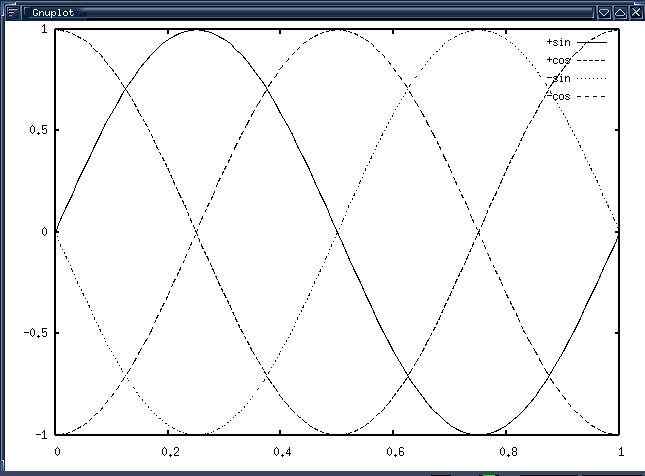
\includegraphics[width=\textwidth]{imagenes/sinus.m.eps}
\caption{M�ltiples l�neas por gr�fica.}
\end{figure}

\begin{ejemplo}{sinus.m}{Presentaci�n  gr�fica  cuatro  sinusoidales.}
Mostramos gr�ficas sobreimpresas entre  ellas y les asignamos t�tulos.
\end{ejemplo}

Octave  y Gnuplot  permiten diferentes  estilos en  las gr�ficas.  Por
ejemplo, en polares, de la forma {\tt polar($\theta$,$\rho$)}:

\begin{figure}[hbtp]
\centering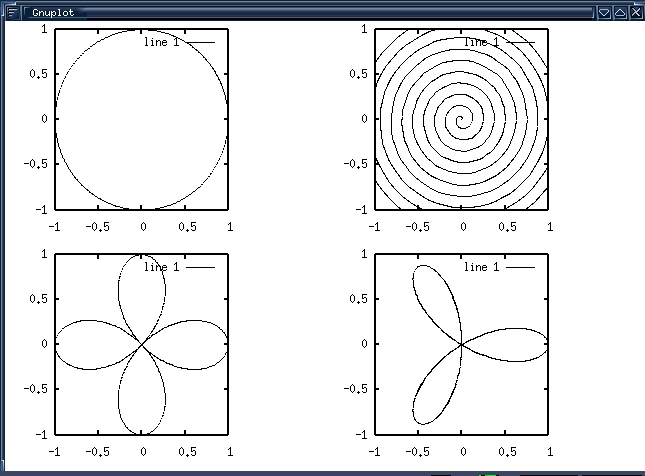
\includegraphics[width=\textwidth]{imagenes/polares.m.eps}
\caption{Diagramas en coordenadas polares}
\end{figure}

\begin{ejemplo}{polares.m}{Presentaci�n gr�fica en polares.}
Mostramos cuatro gr�ficas diferentes en polares en cuatro cuadrantes.
\end{ejemplo}

Tambi�n en forma de histograma, adornando las gr�ficas con t�tulos.

\begin{figure}[hbtp]
\centering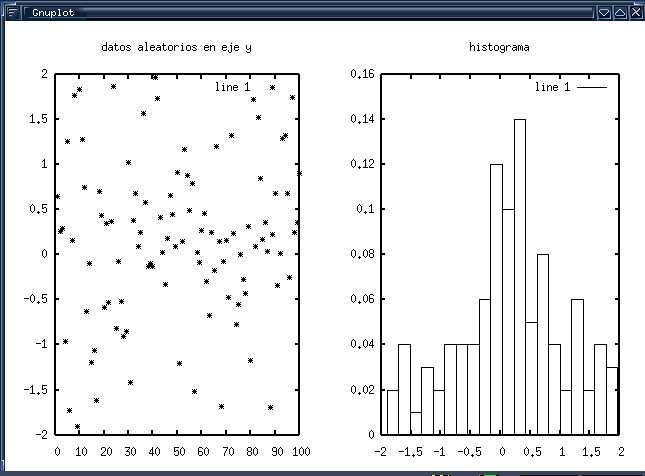
\includegraphics[width=0.9\textwidth]{imagenes/histo.m.eps}
\caption{Representaci�n de histogramas}
\end{figure}

\begin{ejemplo}{histo.m}{Presentaci�n   histograma.}    Mostramos   un
histograma y  sus datos  de partida, con  t�tulos sobre  las gr�ficas.
\end{ejemplo}

\subsection*{Representaci�n en 3D}

La  funci�n {\tt  mesh(x,y,z)} hace  una representaci�n  3D dados  dos
vectores {\tt  x} e {\tt y}  para los ejes y  una matriz bidimensional
{\tt z}  que ser� la coordenada  Z en un espacio  tridimensional. Otra
funci�n  llamada {\tt  contour(x,y,z)} con  los mismos  argumentos que
{\tt mesh()}, dibujar�  las curvas de nivel de la  superficie. En este
ejemplo, lo m�s complicado ser� generar una matriz {\tt z} bonita. Una
vez tenemos la matriz y los ejes, las dos llamadas son directas.

\begin{ejemplo}{meshplot.m}{Gr�fica  en  tres dimensiones.}  Mostramos
una sinc en 3 dimensiones, as�  como los planos usados para generarla.
\end{ejemplo}

\begin{figure}[hbtp]
\centering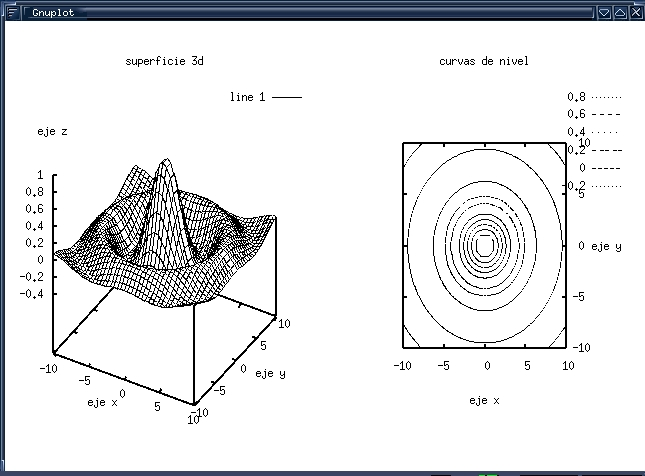
\includegraphics[width=0.8\textwidth]{imagenes/meshplot.m.eps}
\caption{Gr�ficas en tres dimensiones}
\end{figure}

\section{Matrices}
\index{Octave!matrices}
Octave  tiene una  amplia  colecci�n de  funciones  para trabajar  con
matrices y vectores. Las veremos en un ejemplo.

\begin{verbatim}
octave:20> c=diag([1,2,3,4]) # creaci�n de matrices diagonales
c =
  1  0  0  0
  0  2  0  0
  0  0  3  0
  0  0  0  4

octave:21> inv(c) # inversa de una matriz
ans =
  1.00000  0.00000  0.00000  0.00000
  0.00000  0.50000  0.00000  0.00000
  0.00000  0.00000  0.33333  0.00000
  0.00000  0.00000  0.00000  0.25000

octave:22> det(c) # determinante de una matriz
ans = 24

octave:23> eye(4) # matriz identidad de dimensi�n 4
ans =
  1  0  0  0
  0  1  0  0
  0  0  1  0
  0  0  0  1

octave:15> ones(2,3) # matriz 2x3 repleta de unos
ans =

  1  1  1
  1  1  1

octave:16> zeros(1,7) # matriz 1x7 repleta de ceros
ans =

  0  0  0  0  0  0  0

octave:24> rand(4,3) # matriz de n�meros aleatorios 4x3
ans =
  0.85927  0.43700  0.85462
  0.88050  0.27016  0.52905
  0.58098  0.54402  0.29237
  0.41791  0.73324  0.45943

octave:5> randn(3,2) # matriz de n�meros aleatorios gaussiana
ans =

   0.64262  -1.03740
   0.31010  -1.38565
  -0.64096   0.58650

# resta cada elemento con su anterior
octave:7> diff([1 2 4 5 7 9 11 14]) 
ans =

  1  2  1  2  2  2  3

# encuentra �ndices elementos no nulos
octave:8> find ([0 0 0 0 0 0 1 0 0 0 5 0]) 
ans =

   7  11
# subdivide linealmente el intervalo [1,10] en 8 puntos.
octave:9> linspace (1, 10, 8) 
ans =

  1.0000  2.2857  3.5714  4.8571  6.1429  7.4286  8.7143 10.0000

# subdivide logar�tmicamente el intervalo [10^0,10^3] en 6 puntos.
octave:13> logspace (0, 3, 6) 
ans =

   1.0000   3.9811  15.8489  63.0957  251.1886 1000.0000

# factorizaci�n lu de una matriz
octave:26> [a,b,c]=lu([1,3,2;3,2,1;3,2,6]) 
a =

  1.00000  0.00000  0.00000
  0.33333  1.00000  0.00000
  1.00000  0.00000  1.00000

b =

  3.00000  2.00000  1.00000
  0.00000  2.33333  1.66667
  0.00000  0.00000  5.00000

c =

  0  1  0
  1  0  0
  0  0  1

octave:27> [a,b,c]=qr([1,3,2;3,2,1;3,2,6]) # factorizaci�n QR
a =

  -0.312348  -0.752156  -0.580259
  -0.156174  -0.561851   0.812362
  -0.937043   0.344361   0.058026

b =

  -6.40312  -3.12348  -3.59200
   0.00000  -2.69145  -1.40463
   0.00000   0.00000   2.03091

c =

  0  0  1
  0  1  0
  1  0  0


\end{verbatim}


\section{Ecuaciones diferenciales}

\index{Octave!ecuaciones diferenciales}

\begin{ejemplo}{ode.m}{Resuelve una EDO ordinaria}
Resuelve una EDO ordinaria de tercer orden y muestra por pantalla
la evoluci�n de los {\tt x(t)}.
\end{ejemplo}

\begin{figure}[hbtp]
\centering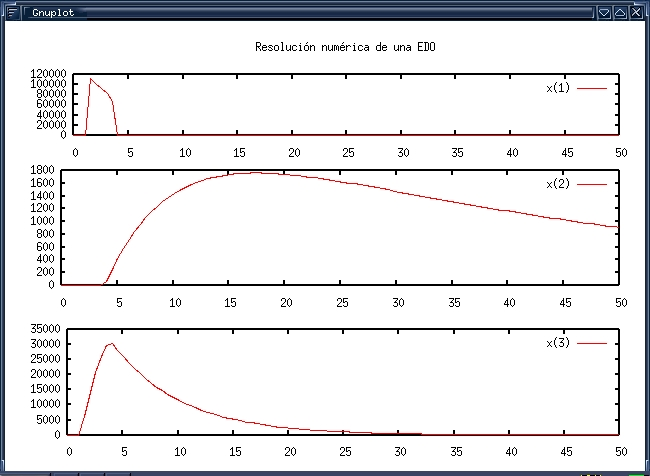
\includegraphics[width=\textwidth]{imagenes/ode.m.eps}
\caption{Resoluci�n num�rica de EDO}
\end{figure}

\section{Polinomios}

\index{Octave!polinomios}

Un  polinomio de  grado r  en  octave se  presenta como  un vector  de
dimensiones $r+1$. A partir de �l se pueden realizar operaciones.

\begin{verbatim}
octave:10> a=[1,2,3]; # a(x)=x^2+2x+3
octave:11> b=[3,2,3,2]; #b(x)=3x^3+2x^2+3x+2
octave:19> polyout(a)
1*s^2 + 2*s^1 + 3
octave:18> polyout(b)
3*s^3 + 2*s^2 + 3*s^1 + 2
octave:20> polyout(conv(a,b)) # producto de polinomios
3*s^5 + 8*s^4 + 16*s^3 + 14*s^2 + 13*s^1 + 6
octave:13> [coc, resto]=deconv([3 8 16 14 13 6],b); # divisi�n
octave:24> polyout (coc) # el cociente de la divisi�n
1*s^2 + 2*s^1 + 3
octave:25> polyout (resto)         # el resto de la divisi�n
0*s^5 + 0*s^4 + 0*s^3 + 0*s^2 + 0*s^1 + 0
octave:26> polyout(polyderiv (b))  # la derivada de b(x)
9*s^2 + 4*s^1 + 3
octave:27> polyout(polyinteg (b))  # la integral de b(x)
0.75*s^4 + 0.666667*s^3 + 1.5*s^2 + 2*s^1 + 0
octave:17> polyval (b,2)           # b(x) evaluado en x=2
ans = 40
\end{verbatim}

% Optimizaci�n: no tengo ni idea.
% Distribuciones estad�sticas: no tengo ni idea.
% Funciones financieras: no tengo ni idea.

\section{Teor�a de control}

\index{Octave!teor�a de control}

La versi�n 2.1 de octave incorpora  una Toolbox de Control. El control
es una rama de la ingenier�a  dedicada a modelar sistemas mediante las
ecuaciones diferenciales  que relacionan  su salida  con su  entrada y
predecir su comportamiento frente a diferentes entradas. En la toolbox
se  utilizan  estructuras para  abstraer  al  usuario el  concepto  de
funci�n de transferencia de un sistema.

% no se si no completar esto porque es muy aburrido y poco vistoso.

\section{Procesamiento de se�ales}

\index{Octave!procesamiento de se�ales}

En esta categor�a  est�n todas las funciones dedicadas  a trabajar con
espectros de se�ales. Tanto la  {\em FFT}, como filtros digitales {\em
FIR} e {\em  IIR}, diferentes tipos de ventanas, o  c�lculo de modelos
ARMA.

La transformada de Fourier discreta, m�s  conocida por el nombre de su
algoritmo FFT ({\bf Fast Fourier Transform}), es la versi�n discreta y
peri�dica de  la transformada exponencial  de Fourier. Es  una funci�n
muy  usada en  ingenier�a y  en  la vida  real. La  tomaremos como  la
funci�n para la ingenier�a por  antonomasia, y en este ejemplo veremos
qu� sencillo  resulta obtener la  transformada de Fourier  discreta de
una senoidal y un pulso.

\begin{ejemplo}{fftview.m}{Muestra  la FFT  de dos  funciones} Muestra
por pantalla el m�dulo y la fase de dos funciones: una sinusoidal (que
debe dar dos deltas de dirac) y un pulso (que debe dar una sinc).
\end{ejemplo}

\begin{figure}[hbtp]
\centering
\subfigure[Ejemplo de FFT aplicado a una sinusoidal]{%
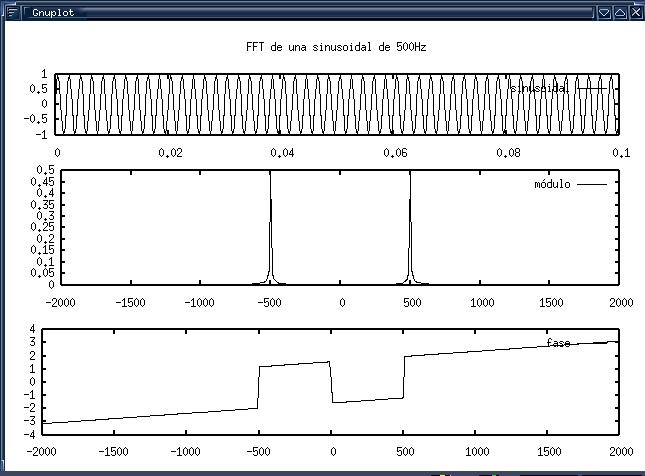
\includegraphics[width=0.8\textwidth]{imagenes/fftview1.m.eps}}
\subfigure[Ejemplo de FFT aplicado a una funci�n escal�n]{%
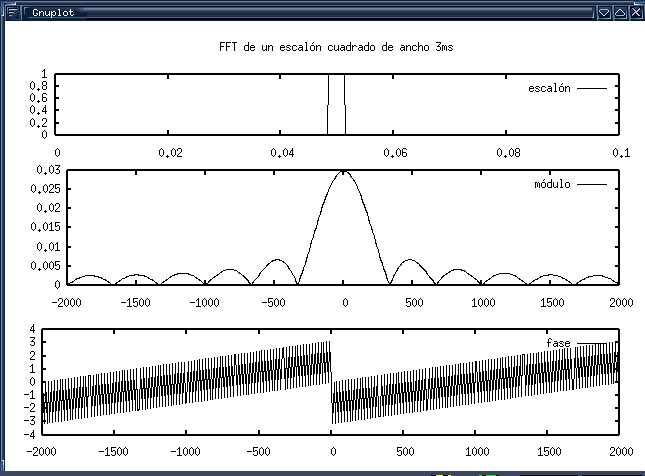
\includegraphics[width=0.8\textwidth]{imagenes/fftview2.m.eps}}
\end{figure}

% estar�a bien poner un filtro de ejemplo, antes y despu�s de pasar
% una se�al por el.

\section{Tratamiento de im�genes}

\index{Octave!tratamiento de im�genes}

Por  �ltimo veamos  un  ejemplo  de c�mo  se  pueden cargar,  realizar
modificaciones,  visualizar y  salvar im�genes  usando las  rutinas de
octave.  Con  esto  podremos  realizar muchas  operaciones  �tiles  en
procesado, realzado y an�lisis de  im�genes, �tiles en muchas �reas de
las ciencias.

En primer lugar suponemos sabido que una imagen se puede entender como
una matriz  donde cada punto tiene  un color diferente. Cada  punto se
llama {\em p�xel}. Hay muchas  formas de representar pixeles, y octave
maneja tres de ellas, que son las siguientes:

\begin{description}

\item[escala de grises]  En una imagen en escala de  grises cada p�xel
se  representa  por  un  valor de  punto  flotante  comprendido  entre
0,  que  significa  negro,  y  1, que  significa  blanco.  Por  tanto,
la  representaci�n  de una  imagen  es  una  matriz llena  de  valores
comprendidos entre 0 y 1. En  este caso, un valor de 0.5 representar�a
un color gris que tiene partes  iguales de blanco y negro mientras que
un valor de  0.2 representar�a un color  que tiene 20\% de  negro y el
resto de blanco.

\item[color RGB] Cualquier  color en la naturaleza  se puede aproximar
(no es una  correspondencia exacta) como suma de  sus tres componentes
de color, a saber:  rojo (R, red), verde (G, green)  y azul (B, blue).
De esta forma, cada p�xel de  una imagen en color se puede representar
como  un terna  de valores  de sus  tres componentes.  Por tanto,  una
imagen en formato  RGB son tres matrices del mismo  tama�o, donde cada
una almacena los valores de una componente.

\item[color  indexado]   Como  en  una  imagen   suele  haber  colores
repetidos,  esta representaci�n  lista  por un  lado  los colores,  de
manera consecutiva y  sin repetirse, y por otro lado  los pixels, cuyo
color  se  almacena  buscando  el  valor en  la  tabla  de  colores  y
almacenando el �ndice correspondiente en el vector.

\end{description}

La  funci�n  usada  para  representar im�genes  en  pantalla  es  {\tt
imshow()}. En  primer lugar  la usaremos  para representar  valores en
escala de grises. Vamos a probar creando una matriz que tenga variedad
de valores y present�ndola. Veamos el ejemplo de uso de esta funci�n:

\begin{verbatim}
octave:15> a=0:0.01:1;
octave:16> ma=a'*a;
octave:17> imshow(ma,2)
octave:18> imshow(ma,16)
octave:19> imshow(ma,256)
\end{verbatim}

\begin{figure}[htbp]
\centering
\subfigure[2 niveles]{%

\includegraphics[width=0.32\textwidth]{imagenes/image1a.m.eps}}
\subfigure[16 niveles]{%

\includegraphics[width=0.32\textwidth]{imagenes/image1b.m.eps}}
\subfigure[256 niveles]{%

\includegraphics[width=0.32\textwidth]{imagenes/image1c.m.eps}}
\caption[Gradiente visualizado a varios niveles de gris]%
{El gradiente anterior visualizado a varios niveles de gris}
\end{figure}

Observando la matriz  {\tt ma} observamos que todos  sus valores est�n
en el  rango $[0,1]$. Si  vemos su tama�o,  vemos que es  100x100. Las
diferentes  llamadas  a {\tt  imshow}  se  diferencian en  el  segundo
par�metro  que representa  el n�mero  de colores  discretos en  el que
presentar� la imagen continua. En el primer caso veremos solamente dos
colores, en la segunda 16 y en la tercera 256.

Probemos ahora  a trabajar con  una imagen  en color. La  funci�n {\tt
loadimage()}  se  utiliza para  cargar  im�genes  de un  archivo.  Las
im�genes se devuelven en formato  indexado, donde {\tt c} representar�
la matriz y {\tt cmap} representar� los colores. Veamos el ejemplo:

\begin{verbatim}
octave:26> [c,cmap]=loadimage("tux.img");
octave:27> imshow(c,cmap)
\end{verbatim}

Como  ver�s, se  visualiza con  la misma  funci�n. Ahora,  usemos esta
imagen como  base para  jugar un poco.  Primero, transform�mosla  a un
formato  m�s  manejable. Empezaremos  pas�ndola  a  {\tt RGB}  con  la
funci�n {\tt ind2rgb}  transforma la imagen de indexada  a RGB. Luego,
con {\tt imshow} la representaremos.

\begin{verbatim}
ctave:28> [r,g,b]=ind2rgb (c,cmap);
octave:29> imshow(r,g,b)
octave:30> imshow(g,r,b)
octave:31> imshow(b,g,r)
\end{verbatim}

\begin{figure}[htbp]
\centering
\subfigure[{\tt imshow(r,g,b)}]{%
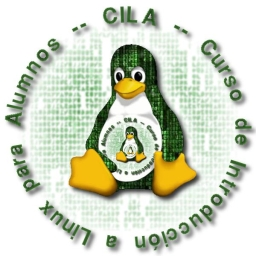
\includegraphics[width=0.32\textwidth]{imagenes/image2a.m.eps}}
\subfigure[{\tt imshow(g,r,b)}]{%
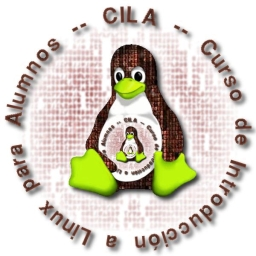
\includegraphics[width=0.32\textwidth]{imagenes/image2b.m.eps}}
\subfigure[{\tt imshow(b,g,r)}]{%

\includegraphics[width=0.32\textwidth]{imagenes/image2c.m.eps}}
\caption[Imagen en color cambiando las componentes RGB]%
{Los colores de la imagen vienen representados por sus componentes
RGB. Si se invierten, los colores cambian.}
\end{figure}

Observamos  que  cada  canal  contiene sus  valores,  y  cambiando  el
orden hacemos  creer a  imshow que  los valores  son diferentes  y nos
muestra im�genes  con los colores trasladados.  Podemos probar tambi�n
sustituyendo las matrices {\tt r}, {\tt g}  o {\tt b} por unos o ceros
y  comprobar el  efecto de  quitar o  a�adir canales.  El trabajo  con
im�genes RGB  es complejo, as�  que usaremos  una imagen en  escala de
grises para seguir efectuando nuestras pruebas.

\begin{verbatim}
octave:32> g=ind2gray (c,cmap);
octave:35> imshow(g,2)
octave:36> imshow(g,4)
octave:37> imshow(g,16)
octave:65> imshow(g,256)
\end{verbatim}

\index{Octave!filtrado de im�genes}

Comenzaremos los an�lisis con  un filtrado/realzado. Estas operaciones
se realizan  barriendo todos  los p�xels  de la  imagen y  creando una
nueva imagen  donde cada p�xel  es una  ponderaci�n de los  valores de
cada  p�xel y  sus vecinos  seg�n unas  matrices preestablecidos.  Las
matrices

\[
\begin{array}{ccc}
\frac{1}{5}\left( \begin{array}{ccc}
0 & 1 & 0\\
1 & 1 & 1\\
0 & 1 & 0
\end{array}\right)  & \left( \begin{array}{ccc}
0 & -1 & 0\\
-1 & 5 & -1\\
0 & -1 & 0
\end{array}\right)  & \left( \begin{array}{ccc}
0 & -1 & 0\\
-1 & 4 & -1\\
0 & -1 & 0
\end{array}\right) \\
\textrm{Filtro pasa-baja} & \textrm{Filtro pasa-alta} & \textrm{Detector de bordes}
\end{array}\]

Ahora veamos como  se aplicar�a un filtro. Este filtro  es el primero,
que  genera una  imagen  donde  cada p�xel  es  un  promedio entre  el
correspondiente en  la imagen original  y sus cuatro vecinos  por cada
lado.

\begin{verbatim}
octave:41> h=zeros(256,256);
octave:42> for i=2:255;
>             for j=2:255;
>                h(i,j)=(g(i,j)+g(i-1,j)+g(i+1,j)+ \
>                       g(i,j-1)+g(i,j+1))/5;
>             endfor;
>          endfor;
octave:43> imshow(g,256)
octave:44> imshow(h,256)
\end{verbatim}

Mostrando la imagen original y  retocada comprobamos que el efecto que
tiene es el de suavizar los bordes de la imagen, el de emborronarla.

Habr�s notado que  has tenido que esperar un rato  (seg�n la velocidad
de  tu  m�quina)   durante  un  buen  rato  para   ver  el  resultado.
Este  procedimiento   es  optimizable  atendiendo  a   las  especiales
caracter�sticas de manejo  de matrices de octave. En vez  de hacer las
operaciones  elemento  a  elemento  con  sus  superiores,  inferiores,
izquierdo  y   derecho,  podemos  hacerlas   globalmente,  simplemente
trabajando con  las matrices  completas y operando  con ellas  con sus
desplazadas una posici�n hacia arriba,  abajo, izquierda y derecha. El
ejemplo esta aqu�  y comprobar�s que el resultado  es notablemente m�s
r�pido.

\begin{verbatim}
octave:44> i=2:255;
octave:45> h=(g(i,i)+g(i-1,i)+g(i+1,i)+g(i,i-1)+g(i,i+1))/5;
octave:46> imshow(g,256)
octave:47> imshow(h,256)
\end{verbatim}

Comprobemos ahora los otros dos filtros. El siguiente filtro pasa-alta
se  implementar�a as�.  El resultado,  al contrario  que el  anterior,
acent�a los bordes en la  imagen, resultando los peque�os detalles m�s
destacados a simple vista.

\begin{verbatim}
octave:44> i=2:255;
octave:45> h=5*g(i,j)-g(i-1,j)-g(i+1,j)-g(i,j-1)-g(i,j+1);
octave:46> imshow(g,256)
octave:47> imshow(h,256)
\end{verbatim}

\begin{figure}[htbp]
\centering
\subfigure[Imagen original]{%

\includegraphics[width=0.32\textwidth]{imagenes/image3a.m.eps}}
\subfigure[Filtro pasa-baja]{%

\includegraphics[width=0.32\textwidth]{imagenes/image3b.m.eps}}
\subfigure[Filtro pasa-alta]{%

\includegraphics[width=0.32\textwidth]{imagenes/image3c.m.eps}}
\caption[Imagen tras aplicarle un filtro pasa-baja y pasa-alta]%
{Cuando aplicamos un filtro pasa-baja se suaviza la imagen y si 
aplicamos un pasa-alta, sus detalles se acent�an.}
\end{figure}

\index{Octave!detecci�n de bordes}

Y por �ltimo, el  detector de bordes, que lo que  hace es presentar de
color blanco  las zonas que en  la imagen original tienen  cambios m�s
r�pidos, mientras que las zonas  m�s homog�neas las presenta en negro.
Con esto, conseguimos detectar bordes acusados en la imagen.

\begin{verbatim}
octave:44> i=2:255;
octave:45> h=5*g(i,j)-g(i-1,j)-g(i+1,j)-g(i,j-1)-g(i,j+1);
octave:46> imshow(g,256)
octave:47> imshow(h,256)
\end{verbatim}

\begin{figure}[hbtp]
\centering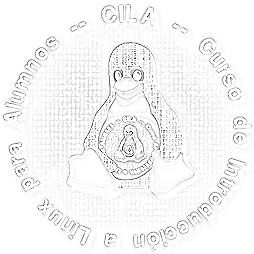
\includegraphics[width=0.8\textwidth]{imagenes/image4.m.eps}
\caption{Imagen tras aplicar detector de bordes.}
\end{figure}

%Autor: amd77

\chapter{GNUplot}


Gnuplot es el programa encargado de hacer  las gr�ficas 2D y 3D que se
visualizaban  en  Octave.  Gnuplot  es un  programa  independiente  de
Octave, que  usado por s�  mismo te permite hacer  representaciones de
funciones  continuas  y  de  tablas  de  datos.  Octave  s�lo  usa  un
subconjunto de las funcionalidades de Gnuplot.

La primera caracter�stica  de Gnuplot es que es muy  similar a Octave
en funcionamiento,  es decir, que  posee una interfaz de  comandos muy
poderosa que  tambi�n puedes utilizar escribiendo  scripts. Esta forma
de trabajar tiene  sus desventajas y sus ventajas.  Las desventajas es
que necesitas  una curva  de aprendizaje m�s  lenta, donde  tienes que
haberte mirado  por lo  menos la  descripci�n de  uno de  los comandos
({\tt plot}) para  poder empezar a hacer algo.  Cuando est�s tanteando
datos mejor que uses otro programa  que te permita hacer las cosas m�s
interactivamente. Pero cuando ya tienes claro lo que tienes que hacer,
por ejemplo, sobre una tabla de datos,  y tienes 100 tablas de datos a
las que hacer  lo mismo, poder hacer  un script puede ser  de una gran
ayuda.

La  otra  caracter�stica  destacable  de Gnuplot  es  la  variedad  de
formatos de  salida de que  dispone, que  se pueden seleccionar  en el
script.  Te permite  exportar  a formatos  vectoriales (xfig,  {\TeX},
postscript),  formatos  bitmap (png,  pbm),  o  formatos de  impresora
(epson, hp, etc).  Con esto puedes tener tu gr�fica  retocada por xfig
en tu publicaci�n en  LaTeX, o bien puesta en tu p�gina  web (png) y o
bien impresa directamente en una impresora.

Al ejecutar gnuplot en un shell entramos a su l�nea de comandos:

\begin{verbatim}
alberto@mencey:~$ gnuplot

	G N U P L O T
	Linux version 3.7
	patchlevel 1
	last modified Fri Oct 22 18:00:00 BST 1999

	Copyright(C) 1986 - 1993, 1998, 1999
	Thomas Williams, Colin Kelley and many others

	Type `help` to access the on-line reference manual
	The gnuplot FAQ is available from
	<http://www.ucc.ie/gnuplot/gnuplot-faq.html>

	Send comments and requests for help to <info-gnuplot@dartmouth.edu>
	Send bugs, suggestions and mods to <submit@bugs.debian.org>


Terminal type set to 'x11'
gnuplot> 
\end{verbatim}

Como fuente  de ayuda teclea  {\tt help}  desde dentro del  programa y
despu�s de una pantalla introductoria te saldr� un prompt sobre el que
podr�s escribir, o bien un nombre que elegir�s de los topics que se te
presentan, o bien un nombre de comando si quieres conocer su sintaxis.

Como has  visto, el formato  de salida es  x11 (visualizar en  las X).
Para ver un listado de los  diferentes tipos de salida disponibles usa
{\tt set terminal}.

\section{Representaci�n de expresiones anal�ticas}

La  parte  m�s sencilla  y  pr�ctica  de  Gnuplot es  la  presentaci�n
de  funciones  continuas, tanto  en  forma  expl�cita {\tt  y=f(x)}  o
{\tt  z=f(x,y)},  como  puede  ser en  forma  param�trica:  curvas  2D
{\tt (x,y)=f(t)},  curvas 3D  {\tt (x,y,z)=f(u)}, superficies  3D {\tt
(x,y,z)=f(u,v)}.

Con  {\tt help  functions} tenemos  un  listado de  las funciones  que
admite. Una  gran desventaja que  tiene es que muestrea  las funciones
a  intervalos  regulares,  por  tanto,  no  hace  ning�n  an�lisis  de
discontinuidades  (lo que  se nota  en, por  ejemplo, la  funci�n {\tt
floor}), aunque s� se puede  configurar para que reduzca el intervalo.
Si queremos  imponer cual ser� el  rango del eje  X o el Y  lo ponemos
entre corchetes antes de la funci�n. Algunos ejemplos:


\begin{verbatim}
gnuplot> plot x                        # identidad
gnuplot> plot abs(x)                   # valor absoluto
gnuplot> plot x**2                     # par�bola
gnuplot> plot [-1:1] sqrt(1-x**2)      # semicircunferencia
gnuplot> plot [] [-0.1:1.1] exp(-x**2) # gaussiana
gnuplot> plot [-1:4] gamma(x)          # funci�n gamma
gnuplot> plot floor(x)                 # funci�n redondeo hacia abajo
gnuplot> plot x-floor(x)               # diente de sierra
gnuplot> splot x**2+y**2               # plot en 3D
gnuplot> splot sqrt(1-x**2+y**2)              
gnuplot> set isosamples 20,20          # cambia la resoluci�n
gnuplot> replot                 
gnuplot> set isosamples 50,50          # cambia la resoluci�n
gnuplot> set contour		       # activa l�neas de nivel
gnuplot> replot
gnuplot> set parametric                # modo param�trico 

	dummy variable is t for curves, u/v for surfaces
gnuplot> set samples 500                   # mejor resoluci�n (+lento)
gnuplot> plot sin(7*t),cos(5*t)            # lissajous en 2D
gnuplot> splot sin(5*u),sin(6*u),sin(7*u)  # lissajous en 3D
gnuplot> set samples 100                   # menor resoluci�n (+r�pido)
gnuplot> splot cos(u)*cos(v),cos(u)*sin(v),sin(u)  # esfera en 3D
\end{verbatim}

\section{Representaci�n de archivos de datos}

 Gnuplot  tambi�n tiene un  modo para trabajar con  archivos de
datos con m�ltiples columnas. Cuando los  archivos de datos tienen 1 �
2  columnas  se  presentan  directamente.  Si  un  archivo  tiene  m�s
de  2 columnas  se  pueden presentar  columnas arbitrariamente,  hacer
operaciones matem�ticas  sencillas entre  columnas. Veamos esto  en un
ejemplo real (bastante prolijo) donde  un servidor genera una l�nea de
log de  load, logins y  carga de cpu, a  cada hora y  queremos obtener
gr�ficas que muestren la evoluci�n en el tiempo 

\begin{verbatim}
# Ejemplo para la monitorizaci�n de carga de un servidor en el tiempo

set title "Convex     November 1-7 1989    Circadian"
set key left box
set xrange[-1:24]
plot 'gnuplot.dat' using 2:4 title "Logged in" with impulses,\
     'gnuplot.dat' using 2:4 title "Logged in" with points
pause -1 "Hit return to continue"

set xrange [1:8]
#set xdtic
set title "Convex     November 1-7 1989"
set key below
set label "(Weekend)" at 5,25 center
plot 'gnuplot.dat' using 3:4 title "Logged in" with impulses,\
     'gnuplot.dat' using 3:5 t "Load average" with points,\
     'gnuplot.dat' using 3:6 t "%CPU used" with lines
set nolabel
pause -1 "Hit return to continue"
reset
\end{verbatim}

 Como �ltimo  ejemplo, vamos a probar un script  donde se hacen
ajustes por el m�todo de m�nimos  cuadrados con Gnuplot. En el ejemplo
se realizan ajustes a una recta  variando los pesos, pero el m�todo de
ajuste que utiliza Gnuplot permite  poner cualquier funci�n de ajuste,
simplemente definiendo las variables y constantes y dando unos valores
iniciales a las constantes. 

\begin{verbatim}
# ajustes por m�nimos cuadrados en Gnuplot 

y(x) = a*x + b   # funci�n a la que se ajustar�
a = 0.0          # valores iniciales
b = 0.0          # de los par�metros

fit y(x) 'gnuplot-fit.dat' via a, b
set title 'Ajuste sin pesar'
plot 'gnuplot-fit.dat', y(x)
pause -1 "Pulsa enter para continuar"

fit y(x) 'gnuplot-fit.dat' using 1:2:3 via a, b
set title 'Ajuste con mayor peso en bajas temperaturas'
plot 'gnuplot-fit.dat', y(x)
pause -1 "Pulsa enter para continuar"

fit y(x) 'gnuplot-fit.dat' using 1:2:4 via a, b
set title 'Ajuste con mayor peso a altas temperaturas'
plot 'gnuplot-fit.dat', y(x)
pause -1 "Pulsa enter para continuar"

fit y(x) 'gnuplot-fit.dat' using 1:2:5 via a, b
set title 'Ajuste con peso correspondiente a error experimental'
plot 'gnuplot-fit.dat' using 1:2:5 with errorbars, y(x)
pause -1 "Pulsa enter para continuar"
\end{verbatim}



%Autor: miguev

\chapter{R}

\index{R}

\section{Introducci�n a R}

%%%%%% Traducido de la web de R en http://www.r-project.org

{\sf R}  es a  la vez un  entorno y un  lenguaje de  programaci�n para
realizar c�lculos y gr�ficos estad�sticos. Es un proyecto GNU similiar
al  sistema {\sf  S}  desarrollado en  Bell Laboratories  (formalmente
AT\&T, ahora  Lucent Technologies)  por John  Chambers y  sus colegas.
{\sf R} puede  considerarse como una implementaci�n  diferente de {\sf
S}. Hay diferencias importantes entre ambos, pero mucho c�digo escrito
para el sistema {\sf S} puede ejecutarse en {\sf R} sin modificarlo.

{\sf  R}  proporciona  una  amplia  variedad de  t�cnicas  gr�ficas  y
estad�sticas (regresiones  lineales y no lineales,  tests estad�sticos
cl�sicos, an�lisis  de series temporales,  clasifiaciones, clustering,
etc.)  y adem�s  es  muy extensible.  El lenguaje  {\sf  S} suele  ser
utilizado para la investigaci�n en  metodolog�a estad�stica, y {\sf R}
proporciona una alternativa de c�digo abierto para esta actividad.

Uno de  los puntos fuertes de  {\sf R} es  la facilidad con la  que se
pueden  producir  gr�ficas  de  buen dise�o  y  calidad  de  imprenta,
incluyendo  s�mbolos y  f�rmulas  matem�ticas  donde sean  necesarias.
Aunque {\sf R}  pone un gran cuidado en las  opciones por defecto para
el dise�o de las gr�ficas, el  usuario puede tener control total sobre
�stas.

{\sf R}  es Software  Libre, disponible  bajo los  t�rminos de  la GNU
General Public  License de  la Free Software  Foundation, en  forma de
c�digo fuente. Se puede compilar y  ejecutar en una amplia variedad de
plataformas  UNIX  (incluyendo  Linux  y  FreeBSD),  MacOS  y  Windows
9x/NT/2000.

El  c�digo  fuente  de  {\sf  R} se  puede  descargar  del  sitio  web
del  proyecto {\sf  R} ({\tt  http://www.r-proyect.org}), as�  como su
documentaci�n. Adem�s de la  documentaci�n oficial (en ingl�s) existen
otros  documentos {\em  contribuidos} entre  los que  se encuentra  la
traducci�n  al  espa�ol  de  ``An Introduction  to  R''  y  ``Gr�ficos
Estad�sticos con R''. \index{R!documentaci�n}  Estos y m�s manuales se
encuentran en el CRAN (Comprehensive R Archive Network), concretamente
en {\tt http://cran.r-project.org/other-docs.html}

%%%%%%

\section{El entorno R}

\index{R!entorno}

{\sf  R} es  un conjunto  integrado de  utilidades para  manipulaci�n,
c�lculo  y  representaci�n  de  datos.  Decimos  que  {\sf  R}  es  un
{\em entorno}  porque es  un sistema  dise�ado para  ser completamente
coherente.  El  entorno  de   {\sf  R}  proporciona  facilidades  para
manipulaci�n  y almacenamiento  de  datos,  operaciones con  variables
indexadas  (como vectores  y matrices),  an�lisis y  representaci�n de
datos, un lenguaje de programaci�n  bien desarrollado (con todo lo que
cabe esperar  de un lenguaje  de programaci�n) y una  amplia colecci�n
integrada y coherente de utilidades para an�lisis de datos.

Aunque mucha  gente utiliza {\sf  R} como un sistema  estad�stico, sus
autores  prefieren considerarlo  como ``un  entorno en  el que  se han
implementado muchas  t�cnicas estad�sticas, cl�sicas y  modernas''. La
mayor�a  de la  estad�stica cl�sica  y muchas  de los  �ltimos m�todos
est�n disponibles en  {\sf R}, aunque posiblemente  tendr�s que buscar
un rato para encontrarlas.

La forma de trabajar  con {\sf R} es distinta a  la de otros programas
como {\tt SPSS}. En {\sf R}, un an�lisis estad�stico se realiza en una
serie de pasos, con unos resultados intermedios que se van almacenando
en  objetos,   para  ser   observados  o   analizados  posteriormente,
produciendo unas salidas  m�nimas. En {\tt SPSS} se  obtendr�a de modo
inmediato  una  salida copiosa  para  cualquier  an�lisis. Esto  puede
parecer a primera  vista una terrible incomodidad,  pero si tuvi�ramos
que  trabajar en  una m�quina  poco potente  r�pidamente nos  dar�amos
cuenta de que puede resultar muy ventajosa la sencillez del entorno de
{\sf  R} (un  entorno de  comandos) y  la posibilidad  de ver  en cada
momento exactamente lo  que se necesita, sin  excesos que desperdicien
recursos del sistema.

A�n as�, la mejor  manera de trabajar con R es  en un entorno gr�fico,
con un sistema de ventanas como  X-Window, de forma que puedas ver las
gr�ficas en el momento de generarlas.

Veamos c�mo se trabaja con {\sf  R} us�ndolo. En primer lugar conviene
crear un  directorio y entrar en  �l antes de comenzar  una sesi�n con
{\sf  R}, que  en  �ste almacena  siempre en  el  directorio donde  se
ejecutan unos ficheros donde almacena  los objetos, datos, funciones y
comandos ejecutados.  Esto puede sernos  muy �til en  trabajos largos,
podemos  interrumpir la  sesi�n con  {\sf  R} en  cualquier momento  y
recuperarla luego donde mismo la dejamos.

Hemos considerado a lo largo de  este curso que el s�mbolo del sistema
Linux/UNIX es  {\tt \$}. Vamos a  considerar ahora que el  s�mbolo del
prompt  {\sf R}  es {\tt  $>$}. \index{R!prompt}  Abre un  emulador de
terminal dentro del entorno gr�fico y ejecuta los siguientes comandos:

\begin{verbatim}
$ mkdir sesion_R
$ cd sesion_R
$ R

R : Copyright 2002, The R Development Core Team
Version 1.5.1  (2002-06-17)

R is free software and comes with ABSOLUTELY NO WARRANTY.
You are welcome to redistribute it under certain conditions.
Type `license()' or `licence()' for distribution details.

R is a collaborative project with many contributors.
Type `contributors()' for more information.

Type `demo()' for some demos, `help()' for on-line help, or
`help.start()' for a HTML browser interface to help.
Type `q()' to quit R.

> 
\end{verbatim}

El prompt de {\sf R} indica  el entorno que est� esperando tus �rdenes
para ejecutarlas. Para salir del entorno de {\sf R} puedes utilizar la
funci�n {\tt q()}  o pulsar {\tt C-d}, entonces {\sf  R} te preguntar�
si  deseas  guardar el  {\em  espacio  de  trabajo},  que es  toda  la
informaci�n sobre la sesi�n que quieres cerrar:

\index{R!sesiones}

\begin{verbatim}
> q()
Save workspace image? [y/n/c]: 
\end{verbatim}

Para salir guardando la sesi�n pulsa {\tt y}, para salir sin guardarla
pulsa {\tt n} y para para cancelar la salida pulsa {\tt c}. Si guardas
la  sesi�n al  salir quedar�  almacenada en  el directorio  en el  que
ejecutaste {\tt R},  y ser� autom�ticamente recuperada  la pr�xima vez
que ejecutes {\tt R} dentro del directorio en cuesti�n.

{\sf R} dispone de un sistema de ayuda similar a las p�ginas de manual
de  Linux/UNIX. Cuando  necesites informaci�n  sobre una  funci�n, por
ejemplo {\tt  solve}, ejecuta la  funci�n {\tt help()}  pas�ndole como
par�metro el nombre de la funci�n que quieras consultar. Tambi�n existe
una forma m�s corta: {\tt ?funci�n}:

\index{R!ayuda}
\index{R!help@{\tt help()}}

\begin{verbatim}
> help (solve)
> ?solve 
\end{verbatim}

Normalmente  puedes  ver  la  documentaci�n tambi�n  en  el  navegador
web. Si  ejecutas {\tt  help.start()} deber�a  abrirse una  ventana de
navegador  con la  documentaci�n en  formato HTML  por la  cual puedes
navegar para buscar lo que necesites.

Otra forma muy interesante de buscar  ayuda dentro del entorno de {\sf
R}  es pasarle  una  palabra  a la  funci�n  {\tt help.search()}.  Por
ejemplo, para buscar  una funci�n que resuelva  sistemas de ecuaciones
puedes empezar por buscar la palabra {\tt solve}.

\index{R!b�squeda}
\index{R!help.search@{\tt help.search()}}

\begin{verbatim}
> help.search ("solve")

Help files with alias or title matching `solve',
type `help(FOO, package = PKG)' to inspect entry `FOO(PKG) TITLE':

backsolve(base)         Solve an Upper or Lower Triangular System
qr(base)                The QR Decomposition of a Matrix
solve(base)             Solve a System of Equations
\end{verbatim}

De un  primer golpe  ya sabes  que el  paquete {\tt  base} de  {\sf R}
tiene  funciones para  resolver  sistemas  triangulares (superiores  o
inferiores), descomponer matrices  en la forma QR  y resolver sistemas
de ecuaciones (cualesquiera).

{\sf  R} proporciona  algunas  demostraciones  sobre sus  capacidades.
Para  ir abriendo  el apetito  ejecuta la  funciones que  muestran las
demostraciones con gr�ficos e im�genes:

\begin{verbatim}
> demo (graphics)
> demo (images)
\end{verbatim}

\begin{figure}[hbtp]
\centering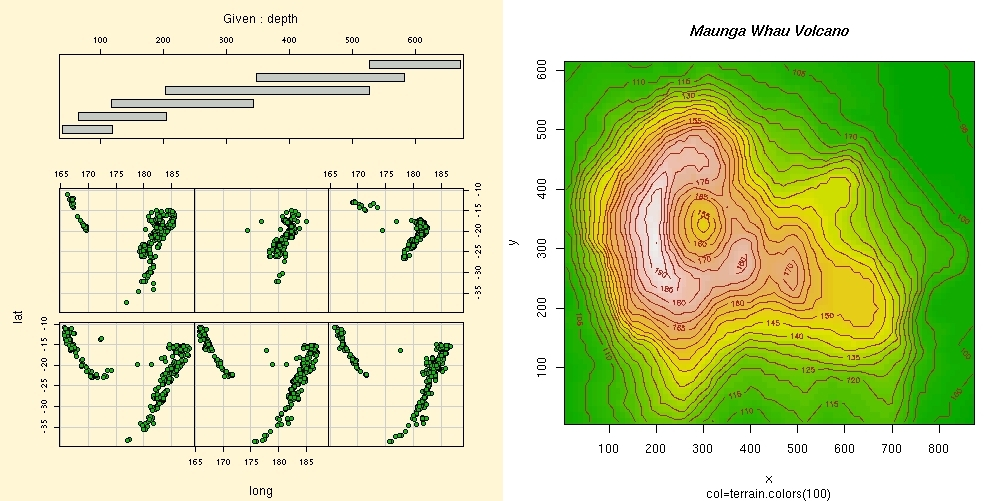
\includegraphics[width=\textwidth]{imagenes/r_demos.eps}
\index{R!demos}
\caption{Demostraciones sobre gr�ficos e im�genes}
\end{figure}


\section{El lenguaje {\sf R}}

\index{R!lenguaje}

{\sf R} es tambi�n lenguaje de  programaci�n en toda regla, con el que
puedes escribir  programas que  procesen ficheros  de datos  y generen
an�lisis y representaciones de los datos.

Al igual que  la mayor�a de lenguajes basados en  UNIX, el lenguaje de
{\sf R} distingue entre may�sculas y min�sculas. Esto es, {\tt esto} y
{\tt  Esto} son  s�mbolos  distintos y  pueden  referirse a  variables
distintas. En {\sf  R} los nombres de variables pueden  tener letras y
n�meros  (como en  casi cualquier  lenguaje), aunque  {\bf no}  pueden
tener el  subrayado ({\tt \_}),  pero en su  lugar s� pueden  tener el
punto.  De hecho  se suele  utilizar  el punto  para separar  palabras
en  los  nombres  de  las  variables en  {\sf  R},  por  ejemplo  {\tt
hoja.de.datos}.

\index{R!�rdenes}
\index{R!comandos}

Las �rdenes  (o comandos) elementales son  expresiones o asignaciones.
Si ejecutas  una expresi�n como comando  �sta se eval�a y  se imprime,
pero su valor se pierde. En una asignaci�n la expresi�n se eval�a y su
valor se almacena en la varbiable, pero no se imprime.

Los comandos se  separan con el caracter  de punto y coma  ({\tt ;}) o
simplemente  con una  salto  de  l�nea. Puedes  agrupar  una serie  de
comandos  encerr�ndolos entre  llaves,  de esta  forma puedes  definir
funciones como veremos m�s adelante. Tambi�n puedes poner comantarios,
\index{R!comentarios} casi  donde quieras\footnote{No puedes  meter un
comentario dentro  de una cadena  de caracteres (formar�a parte  de la
cadena), ni en medio de la lista de argumentos en la definici�n de una
funci�n}, poniendo  una almohadilla ({\tt \#})  y todo lo que  la siga
hasta el final de l�nea ser� obviado por el int�rprete de {\sf R}.

Si dejas  un comando a medias  {\sf R} se  dar� cuenta, y en  lugar de
mostrarte el prompt  $>$ te mostar� {\tt +} para  avisarte de que est�
esperando por el final del comando.

Otra caracter�stica  interesante de {\sf  R} (al menos  en plataformas
Linux/UNIX)  es  la  posibilidad  de  editar  la  l�nea  de  comandos.
Esto  incluye  el  t�pico  historial   de  comandos,  que  te  permite
repetir  los comandos  sin tener  que  volver a  teclearlos. Tan  solo
utiliza los  cursores arriba y  abajo para recuperar los  comandos que
hayas tecleado.  \index{R!historial} Adem�s este historial  de comando
queda  almacenado en  la  sesi�n  cuando sales  del  entorno {\sf  R},
concretamente en  un fichero  {\tt .Rhistory}  en el  directorio donde
ejecutaste en entorno {\sf R}.

Pero si necesitas usar una serie un poco larga de comandos seguramente
te canses de tener  que darle a los cursores. Para  estos casos lo que
necesitas  es un  script en  el que  escribes los  comandos a  modo de
programa. Luego para ejecutar los  comandos escritos en �l utilizas la
funci�n {\tt  source ()} del  entorno pas�ndole el nombre  del fichero
donde escribiste los comandos:

\index{R!leer comandos de un fichero}
\index{R!source@{\tt source()}}

\begin{verbatim}
> source ("script.R")
\end{verbatim}

Del  mismo modo  que puedes  tomar la  entrada de  un fichero  tambi�n
puedes redireccionar la salida hacia otro fichero, con la funci�n {\tt
sink()}. Para almacenar la salida en el fichero {\tt salida.txt} 
ejecuta el comando:

\index{R!volcar en un fichero}
\index{R!sink@{\tt sink()}}

\begin{verbatim}
> sink ("salida.txt")
\end{verbatim}

Para devolver  la salida al  int�rprete utiliza la misma  funci�n {\tt
sink  ()}  pero sin  pasarle  ning�n  par�metro.  En el  fichero  {\tt
iodemo.R}  tienes un  ejemplo de  esto. Entra  en el  directorio donde
tengas el fichero y ejecuta en el entorno {\sf R}

\begin{verbatim}
> source ("iodemo.R")
\end{verbatim}

Este gui�n (serie de comandos) lee una tabla que est� almacenada en un
fichero  de texto  llano  ({\tt muestra.dat},  que  usaremos para  los
ejemplos) y extrae dos variables de ella. Para ambas variables muestra
un  breve resumen  estad�stico, pero  guarda  uno en  el fichero  {\tt
salida.txt} y el otro lo muestra en el entorno {\sf R}.


\section{Vectores}

\index{R!vectores}

{\sf R} realiza las operaciones sobre las llamadas {\em estructuras de
datos}, de las cuales la m�s  simple es el vector num�rico. Para crear
un vector con  los 5 primeros n�meros enteros  positivos utilizamos la
funci�n {\tt  c()} que  combina los objetos  recibidos para  formas un
vector:

\begin{verbatim}
> x <- c (1, 2, 3, 4, 5)
> x
[1] 1 2 3 4 5
\end{verbatim}

\index{R!asignaci�n, operador de}

En efecto, el operador de asignaci�n no se parece para nada a un signo
de igualdad. De  hecho es una flecha, que est�  indicando que el valor
de lo que hay a su derecha debe asignarse a lo que hay a su izquierda.
Si le das la vuelta a la flecha funciona al rev�s:

\begin{verbatim}
> c (6, 7, 8, 9, 10) -> y
> y
[1]  6  7  8  9 10
\end{verbatim}

Cuando  ejecutas  el  nombre  de  un  objeto  como  comando,  {\sf  R}
interpreta que deseas  ver su contenido y entonces  ejecuta la funci�n
{\tt print()} sobre  el objeto en cuesti�n. Esto  funciona s�lo cuando
est�s  dentro del  entorno {\sf  R} y  tecleas el  nombre del  objeto.
\index{R!print@{\tt print()}}
Cuando quieras imprimir  el objeto desde un fichero  de comandos (como
hacemos en {\tt iodemo.R}) has de utilizar la funci�n {\tt print()}.

Dado que la funci�n {\tt c()} combina objetos para formar vectores, 
tambi�n puede combinar varios vectores para formar un nuevo vector
que es el resultado de concatenar los anteriores:

\begin{verbatim}
> z <- c (x, y)
> z
 [1]  1  2  3  4  5  6  7  8  9 10
\end{verbatim}

Las  operaciones  usuales  entre  vectores  se  definen  ``elemento  a
elemento'':

\index{R!vectores!operaciones elementales}

\begin{verbatim}
> x + 2
[1] 3 4 5 6 7
> 2 * x
[1]  2  4  6  8 10
> x + y
[1]  7  9 11 13 15
> x - y
[1] -5 -5 -5 -5 -5
> x * y
[1]  6 14 24 36 50
> x / y
[1] 0.1666667 0.2857143 0.3750000 0.4444444 0.5000000
> y / x
[1] 6.000000 3.500000 2.666667 2.250000 2.000000
> x ^ y
[1]       1     128    6561  262144 9765625
> y ^ x
[1]      6     49    512   6561 100000
\end{verbatim}

Pero  entonces �c�mo  se multiplican  escalarmente dos  vectores? Para
esto hay una funci�n llamada  {\tt crossprod}, que permite multiplicar
dos  vectores  (o  matrices).  El operador  \verb|%*%|  es  una  forma
abreviada  de  este  producto.  Formalmente  {\tt  crossprod(x,y)}  es
equivalente a  {\tt t(x) \%*\%  y}, pero  m�s r�pido. La  funci�n {\tt
t()} es la trasposici�n de matrices:

\index{R!vectores!producto escalar}

\begin{verbatim}
> x
[1] 1 2 3 4
> y
[1] 4 5 6 7
> crossprod(x,y)
     [,1]
[1,]   60
> x %*% y
     [,1]
[1,]   60
\end{verbatim}

Adem�s de para guardar datos,  los vectores suelen usarse para definir
series o  secuencias. Para  definir una  secuencia de  n�meros enteros
consecutivos basta  con poner el primer  y el �ltimo separados  por un
caracter de dos puntos:

\index{R!vectores!secuencias}

\begin{verbatim}
> x <- 1:10
> x   
 [1]  1  2  3  4  5  6  7  8  9 10
\end{verbatim}

Pero  para  generar   secuencias  la  mejor  manera   es  utilizar  la
funci�n {\tt  seq()}. Si  le pasas tres  valores num�ricos  le estar�s
especificando el  primer y el  �ltimo elemento  de la secuencia,  y la
diferencia que debe haber entre cada dos elementos consecutivos:

\begin{verbatim}
> y <- seq (-1, 1, .2)
> y
 [1] -1.0 -0.8 -0.6 -0.4 -0.2  0.0  0.2  0.4  0.6  0.8  1.0
\end{verbatim}

Para replicar  un objeto  varias veces, por  ejemplo para  generar una
secuencia  peri�dica,  utiliza la  funci�n  {\tt  rep()} pas�ndole  el
objeto y el n�mero de veces que quieres replicarlo:

\begin{verbatim}
> z <- rep (seq (-1, 1, 1), 5)
> z
 [1] -1  0  1 -1  0  1 -1  0  1 -1  0  1 -1  0  1
\end{verbatim}

Adem�s de vectores num�ricos, {\sf R} permite operar con vectores {\em
l�gicos}.  Los valores  v�lidos  para los  elementos  de los  vectores
\index{R!vectores!vectores l�gicos}
l�gicos son los de la {\em l�gica  triestada}: 
\index{l�gica triestada}
{\tt TRUE}, {\tt FALSE} y {\tt NA} (``Not Available'', no disponible).
Los operadores  l�gicos para manejar  estos valores son {\tt  \&} para
``and'', {\tt |} para ``or'' y {\tt !} para ``not''.

Una forma  de generar  un vector  de valores  l�gicos es  efectuar una
comparaci�n entre un vector num�rico y un valor num�rico:

\begin{verbatim}
> z <- rep (seq (-1, 1, 1), 3)
> z
[1] -1  0  1 -1  0  1 -1  0  1
> z > 0
[1] FALSE FALSE  TRUE FALSE FALSE  TRUE FALSE FALSE  TRUE
\end{verbatim}

Al contrario que  en la mayor�a de lenguajes de  programaci�n, en {\sf
R}  los vectores  se indexan  comenzando por  $1$. Para  acceder a  un
elemento  de un  vector utiliza  la notaci�n  usual de  los corchetes.
Tambi�n puedes acceder a un  subconjunto del vector especificando como
�ndice un vector con las posiciones de los elemenos:

\index{R!vectores!�ndices}
\index{R!vectores!sub�ndices}
\index{R!vectores!indixado}

\begin{verbatim}
> x <- 1:10
> x
 [1]  1  2  3  4  5  6  7  8  9 10
> x[2:5]
[1] 2 3 4 5
> x[8:2]
[1] 8 7 6 5 4 3 2
\end{verbatim}

Tambi�n puedes  acceder a  un subconjunto de  un vector  utilizando un
vector l�gico:

\begin{verbatim}
> x[x > 4]
[1]  5  6  7  8  9 10
\end{verbatim}

Incluso puedes indexar  un vector no palabras, poniendo  nombres a las
posiciones dentro del vector mediante  la funci�n {\tt names()}. Luego
puedes acceder a los elementos mediante los nombres de las posiciones:

\index{R!vectores!nombres}
\index{R!vectores!names@{\tt names()}}

\begin{verbatim}
fruta = c (5, 10, 1, 20)
> fruta <- c (5, 10, 1, 20)
> names (fruta) <- c ("naranja", "pl�tano", "manzana", "�ame")
> fruta[c ("manzana", "naranja")]
manzana naranja 
      1       5 
> fruta
naranja pl�tano manzana    �ame 
      5      10       1      20 
\end{verbatim}

\section{Arrays y matrices}

\index{R!arrays}
\index{R!matrices}

Un   {\em   array}\footnote{a   veces   traducido   por   ``arreglo''}
\index{arreglo} es  una variable indexada multidimensional.  Un vector
es un  array unidimensional  y una matriz  es un  array bidimensional.
{\sf R} proporciona un buen manejo de arrays, sobretodo para matrices.

La dimensi�n de un array es un vector cuya longitud es la dimesi�n del
array,  y  cada uno  de  sus  elementos  es  la ``longitud''  de  cada
dimensi�n en el array. Por  ejemplo, un array con dimesi�n $(3,5,100)$
ser�a como un cubo de $1500$ elementos con $3$ celdas de largo, $5$ de
ancho y $100$ de alto.

\index{R!arrays!dimensi�n}

En la  mayor�a de  lenguajes los  elementos de  un array  se almacenan
``por filas'', lo que significa que el �ndice que avanza m�s r�pido es
el �ltimo. Sin embargo, en {\sf R}  la ordenaci�n se hace al estilo de
FORTRAN, ordenando  los elementos  ``por columnas'', lo  que significa
que el �ndice que avanza m�s r�pido es el primero.

Es importante tener esto en cuenta porque a la hora de crear una 
matriz hay que proporcionar los elementos agrupados por columnas, no 
por filas. Por ejemplo:

\index{R!arrays!por filas}
\index{R!arrays!por columnas}


\begin{verbatim}
> a <- array (c (1:3,-3:-1), dim = c (3,2)) 
> a
     [,1] [,2]
[1,]    1   -3
[2,]    2   -2
[3,]    3   -1
\end{verbatim}

Para  acceder a  los elementos  de una  matriz (o  array) ponemos  los
sub�ndices  entre corchetes  y  separados por  comas.  Si omitimos  el
sub�ndice de las filas (el  primero) obtenemos la columna se�alada por
el segundo sub�ndice, y an�logamente  obtenemos las filas omitiendo el
segundo sun�ndice.

\index{R!arrays!�ndices}
\index{R!arrays!sub�ndices}
\index{R!arrays!indexado}

\begin{verbatim}
> a[1,2]
[1] -3
> a[,2]
[1] -3 -2 -1
> a[1,]
[1]  1 -3
\end{verbatim}

De la misma forma que podemos extraer elementos, filas o columnas de
una matriz tambi�n podemos asignarles valores:

\begin{verbatim}
> a[,2] <- 3:5
> a[,2]
[1] 3 4 5
> a
     [,1] [,2]
[1,]    1    3
[2,]    2    4
[3,]    3    5
\end{verbatim}

Para multiplicar  matrices (o arrays  en general) utiliza  el operador
\verb|%*%| que vimos antes:

\index{R!arrays!producto}
\index{R!matrices!multiplicar}

\begin{verbatim}
> a
     [,1] [,2]
[1,]    1    3
[2,]    2    4
[3,]    3    5
> b = array (1:2, 2:1, dim = c (2,2))
> b
     [,1] [,2]
[1,]    1    1
[2,]    2    2
 %*% b
     [,1] [,2]
[1,]    7    7
[2,]   10   10
[3,]   13   13
\end{verbatim}

Vimos antes  que si multiplicamos dos  vectores {\tt x} y  {\tt y} (de
igual longitud) utilizando el operador  {\tt \%*\%} el resultado es el
producto  escalar de  los vectores.  En realidad  la operaci�n  {\tt x
\%*\%  y}  es ambigua,  porque  podr�a  significar  $x'  x$ o  $x  x'$
(considerando $x$ un vector columna).  En estos casos de ambig�edad se
considera impl�citamente  que la interpretaci�n deseada  es aquella de
la  que resulte  la  matriz m�s  paque�a,  por lo  que  se obtiene  el
producto escalar $x' x$.

Para  calcular la  matriz $x  x'$ puedes  utilizar las  funciones {\tt
cbind()} y {\tt rbind()}, ya que �stas siempre devuelven matrices. Las
funciones {\tt  cbind} y  {\tt rbind}  toman una  serie de  vectores o
n�meros y los agrupan por columnas o filas en una matriz.

\index{R!matrices!cbind@{\tt cbind()}}
\index{R!matrices!rbind@{\tt rbind()}}

\begin{verbatim}
> x
[1] 1 2 3 4
> y
[1] 4 5 6 7
> x %*% y
     [,1]
[1,]   60
> cbind(x,y)
     x y
[1,] 1 4
[2,] 2 5
[3,] 3 6
[4,] 4 7
> rbind(x,y)
  [,1] [,2] [,3] [,4]
x    1    2    3    4
y    4    5    6    7
> cbind(x) %*% rbind(y)
      
       [,1] [,2] [,3] [,4]
  [1,]    4    5    6    7
  [2,]    8   10   12   14
  [3,]   12   15   18   21
  [4,]   16   20   24   28
\end{verbatim}


\section{Factores: clasifici�n de datos}

\index{R!factores}
\index{R!clasificaci�n de datos}

Un  {\em factor}  es un  vector  que utilizamos  para especificar  una
clasificaci�n  discreta (agrupamiento)  de  los  componentes de  otros
vectores del mismo tama�o. Para entender  lo que son los factores nada
mejor que un ejemplo claro y sencillo. En el entorno {\sf R} y ejecuta
lo siguiente:

\begin{verbatim}
> edad <- c (13, 16, 15, 17, 17, 18, 16, 16, 15, 16)
> sexo <- c ("hombre", "hombre", "mujer", "hombre", "mujer", "mujer",         
+            "hombre", "mujer", "hombre", "mujer") 
> edad
 [1] 13 16 15 17 17 18 16 16 15 16
> sexo
[1] "hombre" "hombre" "mujer"  "hombre" "mujer"  "mujer"  "hombre" "mujer" 
[9] "hombre" "mujer"
\end{verbatim}

Ahora tienes  una variable {\tt  Edad} que  contiene las edades  de 10
personas, y  una variable {\tt  Sexo} que define  el sexo de  cada una
de  las  10  personas  anteriores  (en el  mismo  orden)  y  que  toma
�nicamente  los  valores  \verb|"hombre"| y  \verb|"mujer"|.  Vamos  a
calcular  la media  y  la  varianza muestrales  de  la  edad de  estas
personas  clasific�ndolas seg�n  el sexo,  i.e. la  edad media  de los
hombres por un lado y la de las mujeres por otro.

Necesitamos  separar (agrupar)  los  elementos del  vector {\tt  edad}
seg�n los valores que toma el  vector {\tt sexo}. Para esto utilizamos
un factor.  El factor  en realidad  es como  el vector  original, pero
tiene un atributo  a�adido llamado {\tt levels} (niveles)  que son los
distintos  valores que  toman los  elementos del  vector original.  En
el  caso del  vector  {\tt  edad} los  niveles  son \verb|"hombre"|  y
\verb|"mujer"|. La funci�n  {\tt levels} devuelve la  lista de niveles
que tenga el factor que le pases como par�metro.

\begin{verbatim}
> sexo.factor = factor (sexo)
> sexo.factor
[1] hombre hombre mujer  hombre mujer  mujer  hombre mujer  hombre
Levels:  hombre mujer 
> levels (sexo.factor)
[1] "hombre" "mujer"
\end{verbatim}

Ahora queremos  aplicar unas  funciones, en este  caso {\tt  mean()} y
{\tt  var()}, a  un  vector de  datos  de manera  que  los datos  sean
separados seg�n  un factor.  La funci�n apropiada  para esta  tarea es
{\tt tapply}, y se usa del siguiente modo:

\index{R!tapply@{\tt tapply()}}

\begin{verbatim}
> tapply (edad, sexo.factor, mean)
hombre  mujer 
  15.4   16.4 
> tapply (edad, sexo.factor, var)
hombre  mujer 
   2.3    1.3
\end{verbatim}

As� obtenemos que dentro de esta muestra de 10 personas, la edad media
de los hombres es $15.4$ y  la de las mujeres $16.4$. Volveremos sobre
los factores m�s adelante, as� que aseg�rate de entender al menos este
uso de los mismos. Para mayores detalles consulta la ayuda de {\sf R}.

\section{Listas}

\index{R!listas}

En un  array todos  los elementos  deben ser del  mismo tipo,  i.e. no
puede  ser que  un array  contenga a  la vez  n�meros y  palabras. Sin
embargo la  mayor�a de muestras  contienen datos de  diferentes tipos:
n�meros, palabras, valores l�gicos, intervalos, etc.

Una {\em  lista} en {\sf  R} es una  colecci�n ordenada de  objetos de
cualquier tipo. Es  como un vector, pero con la  diferencia de que sus
elementos pueden ser de distintos tipos. 

Los elementos de una lista est�n  siempre numerados por un sub�ndice y
puedes referirte  a ellos  como con un  vector, pero  usando corquetes
dobles.  As�  si {\tt  L}  es  una lista  {\tt  L[[1]]}  es su  primer
elemento. Pero tambi�n,  al igual que en los  vectores, puedes indexar
los elementos  de una lista d�ndoles  nombres. En caso de  nombrar los
elementos de una lista hay una  forma m�s c�moda de referirse a ellos:
en lugar de {\tt L[["nombre"]]} puedes usar {\tt L\$nombre}.

\index{R!listas!�ndices}
\index{R!listas!nombres}

\begin{verbatim}
> L = list (nombre = "Pepe", esposa = "Pepa", hijos = 3,
+     edades.hijos = c (34,6,12))
> L
$nombre
[1] "Pepe"

$esposa
[1] "Pepa"

$hijos
[1] 3

$edades.hijos
[1] 34  6 12

> L[["nombre"]]
[1] "Pepe"
> L$nombre
[1] "Pepe"
\end{verbatim}

Para concatenar  listas recuerda que  la funci�n {\tt c()}  sirve para
ello.

\section{Hojas de datos}

\index{R!tablas}
\index{R!data frame}
\index{R!frame}
\index{R!hojas de datos}

Una ``hoja  de datos'' (en  ingl�s ``data frame'') es  b�sicamente una
lista de vectores, con algunas restricciones. Los vectores de palabras
son convertidos en factores.

Piensa en una hoja  de datos como su nombre sugiere:  una hoja o tabla
en la que tienes varios datos sobre varios individuos. Las columnas de
la hoja de  datos son los vectores  que la format, y cada  fila es una
lista.

En el  fichero {\tt  muestra.dat} tienes una  hoja de  datos preparada
para ser leida con la funci�n  {\tt read.table()}. La primera fila son
los nombres  de los vectores columna,  y luego cada l�nea  del fichero
introduce  una lista  de  valores,  un valor  para  cada vector.  Para
entender esto con claridad lee  la tabla del fichero {\tt muestra.dat}
y mantenla en una variable:

\index{R!hojas de datos!leer desde fichero}
\index{R!read.table@{\tt read.table()}}

\begin{verbatim}
> hoja.datos = read.table ("muestra.dat") 
> names (hoja.datos)
[1] "Sexo"     "Edad"     "Habitat"  "Ingresos" "Lectura"  "TV"
\end{verbatim}

Esta tabla contiene  los datos (ficticios) de 50 j�venes:  su sexo, su
edad,  su  h�bidat,  sus  ingresos familiares  (en  miles  de  pesetas
mensuales),  el n�mero  de libros  leidos  anualmente y  sus horas  de
televisi�n diarias.

Normalmente para  acceder al  vector {\tt  Edad} de  la hoja  de datos
utilizar�amos la expresi�n {\tt  hoja.datos\$Edad}, pero hay una forma
m�s c�moda. Consiste en ``conectar'' la hoja de datos para que puedas
referirte a sus vectores directamente por su nombre:

\index{R!hojas de datos!conectar}

\begin{verbatim}
> attach (hoja.datos)
> summary (Edad)
   Min. 1st Qu.  Median    Mean 3rd Qu.    Max. 
  12.00   15.00   16.00   15.64   17.00   20.00
\end{verbatim}

Ten en cuenta que  este atajo es s�lo para {\em leer}  los datos de la
hoja, no para modificarlos. Si quieres  modificar un vector de la hoja
de datos tienes que usar la notaci�n normal:

\begin{verbatim}
> hoja.datos$Edad <- Edad + 10
\end{verbatim}

De hecho, esto modifica  el vector en la hoja de  datos, pero no ver�s
los cambios en los atajos hasta que  desconectes la hoja de datos y la
vuelvas  a conectar.  Para desconectar  una hoja  de datos  utiliza la
funci�n {\tt detach()}.

\index{R!hojas de datos!desconectar}

Cuando quieras  almacenar una hoja de  datos en un fichero  utiliza la
funci�n {\tt write.table()}. Su uso b�sico es darle la hoja de datos y
el nombre del  fichero, pero admite varias  opciones para personalizar
la  forma en  la  que escribir�  los  datos en  el  fichero. Para  ver
estos  detalles consulta  la ayuda  sobre la  funci�n ejecutando  {\tt
?write.table}. \index{R!hojas de datos!escribir en fichero}

\subsection{Valores perdidos}

\index{R!valores perdidos}

En ocasiones  te encontrar�s  con hojas de datos  en las  que alguna
celda no tiene el dato. Esto puede suceder porque no haya sido posible
averiguar el dato,  o porque �ste no tenga sentido.  En estos casos se
utiliza para esa  celda el valor {\tt NA}, que  significa que el valor
``no est� disponible'' (NA es abreviatura de ``Not Available'').

\index{R!NA@{\tt NA}}

En otros casos sucede que tras efectuar una serie de operaciones sobre
un  conjunto de  datos algunos  de  los resultados  no tengan  sentido
matem�tico, como  por ejemplo una  divisi�n por cero (recuerda  que la
precisi�n  de los  procesadores es  limitada).  En caso  de hacer  una
operaci�n as� {\sf R} no se quejar� en absoluto, sino que devolver� el
valor {\tt  NaN} que  significa que  eso ``no es  un n�mero''  (NaN es
abreviatura de ``Not a Number'').

\index{R!NaN@{\tt NaN}}

\section{Funciones}

\index{R!funciones}

Como todo  buen lenguaje de  programaci�n, {\sf R} te  permite definir
funciones  para tu  uso propio.  Para definir  una funci�n  asignas al
objeto (que  ser� tu funci�n)  el valor  devuelto por la  funci�n {\tt
function}. Esta  funci�n particular  recibe los mismos  par�metros que
recibir�  tu  funci�n,  y  a  continuaci�n  una  {\em  agrupaci�n}  de
comandos, encerrados entre llaves y separados  con {\tt ;} o saltos de
l�nea. El  valor devuelto por  tu funci�n ser�  el valor de  la �ltima
expresi�n de la agrupaci�n.

Por ejemplo  si quieres  una funci�n  que calcule  la curtosis  de una
muestra:

\begin{verbatim}
> curtosis <- function (x) {
+ n <- length (x)
+ c <- ( (n * (n - 1) * sum((x - mean(x))^4) ) /
+      ( (n - 1) * (n - 2) * (n - 3) * (var(x))^4 ) ) -
+      ( (3 * (n - 1)^2) / ( (n - 2) * (n - 3) ) )
+ c 
+ }
> hoja.datos = read.table ("muestra.dat")
> attach (hoja.datos)
> curtosis (Edad)
[1] -2.921993
> curtosis (Lectura)
[1] -3.191575
> curtosis (TV)
[1] -3.192770
\end{verbatim}

Normalmente las funciones no quedan bien escritas a la primera, por lo
que tendr�s que corregirlas una y  otra vez. O tal vez quieras definir
m�s funciones,  modificar las que  ya tengas escritas, etc.  Todo esto
puedes hacerlo m�s c�modamente si escribes las funciones en un fichero
y lo importas con la funci�n {\tt source()} que vimos antes.

\index{R!funciones!leer desde fichero}

As� por ejemplo tienes escrita la funci�n {\tt curtosis} en el fichero
{\tt curtosis.R}. Si quieres modificarla  y volver a usarla despu�s de
modificada no  hay problema.  Edita el  fichero {\tt  curtosis.R} para
modificar la funci�n  y luego vuelve a importarlo con  la funci�n {\tt
curtosis}. Recuerda que la funci�n {\tt curtosis} ejecuta los comandos
que encuentra en el fichero que le digas, por lo que las funciones que
tengas escritas en  el fichero ser�n redefinidas y  estar�n lista para
usar al instante.

% NO TE OLVIDES DE ESTO

\subsection{Control de flujo}

\index{R!funciones!control de flujo}

{\sf R} proporciona la sintaxis necesaria para construir funciones que
mantengan  en control  del flujo  del  programa. Nos  referimos a  los
condicionales y los bucles:

\subsubsection*{Ejecuci�n condicional}

\index{R!funciones!if@{\tt if}}

La  forma  de  contruir  una  sentencia  condicional  en  {\sf  R}  es
{\tt  if (expresion\_logica)  sentencia\_1 else  sentencia\_2}. Si  la
{\tt  expresion\_logica}  es  cierta  (su  valor  es  {\tt  TRUE})  se
ejecutar� la  {\tt sentencia\_1},  en otro caso  se ejecutar�  la {\tt
sentencia\_2}.  {\tt sentencia\_1}  y  {\tt  sentencia\_2} pueden  ser
tambi�n agrupaciones de comandos y/o expresiones.

\begin{verbatim}
> x = 1      
> y = 2
> if (x > y) x else y
[1] 2
\end{verbatim}

En las  expresiones booleanas  puedes emplear  los operadores  {\tt |}
(OR) {\tt \&}  (AND) y {\tt !} (NOT) normales,  o si prefieres ahorrar
un poco de  tiempo los operadores ``cortocicuitados'' {\tt  ||} (OR) y
{\tt  \&\&}.  \index{R!||@{\tt  ||}} \index{R!\&\&@{\tt  \&\&}}  Estos
operadores l�gicos  tienen la ventaja  de que s�lo eval�an  la segunda
expresi�n cuando es necesario.

Para las  comparaciones num�ricas se utilizan  los mismos comparadores
binarios que en el lenguaje C:  {\tt $<$}, {\tt $>$}, {\tt $<=$}, {\tt
$>=$}, {\tt  !=} y {\tt  ==}. Ten cuidado  de no utilizar  el operador
{\tt =} para comparaciones.

\index{R!funciones!ifelse@{\tt ifelse()}}

Existe  adem�s  una  versi�n   {\em  vectorizada}  de  la  construci�n
condicional. Se trata  de la funci�n {\tt ifelse ()},  que recibe tres
vectores {\tt condicion, a, b} y devuelve un vector del tama�o del m�s
largo.  En este  vector  el  elemnto i-�simo  es  {\tt  a[i]} si  {\tt
condicion[i]} es cierto (su valor es {\tt TRUE}) o bien {\tt b[i]}) en
caso contrario.

\begin{verbatim}
> condicion = c (TRUE, FALSE)
> a = c (1, 2)
> b = c (3, 4)
> ifelse (condicion, a, b)
[1] 1 4
\end{verbatim}

\subsubsection*{Ejecuci�n repetitiva}

\index{R!funciones!for@{\tt for}}

Para la ejecuci�n  repetitiva de comandos dispones  de la construcci�n
{\tt for (variable in valores)  comandos}, donde {\tt variable} es una
variable vac�a  que ir� cambiando  de valor en cada  iteraci�n tomando
consecutivamente los valores  del vector {\tt valores}.  Para cada uno
de estos valores se ejecutar� la secuencia {\tt comandos}.

\begin{verbatim}
> for (i in 1:3) print (c (i^2, i^3, i^4, i^5))
[1] 1   1   1   1
[1] 4   8  16  32
[1] 9  27  81 243
\end{verbatim}

\index{R!funciones!while@{\tt while}}

Para ejecutar  una secuencia  {\em mientras}  se cumpla  una condici�n
(podr�a no  ejecutarse la  primera vez)  utiliza la  construcci�n {\tt
while (condicion)  comandos}. As�  mientras el  valor de  la expresi�n
{\tt condicion} sea {\tt TRUE} se seguir� ejecutando la secuencia {\tt
comandos}.

\begin{verbatim}
x = rnorm (1)
> while (x > -2) {
+   print (x)
+   x = rnorm (1)
+ }
[1] -0.2199842
[1] -0.1615499
[1] 2.580791
[1] -0.1202099
[1] -0.794566
[1] -1.413912
[1] 0.4829018
[1] 0.2780835
[1] -0.5475556
[1] 2.974901
[1] -0.1805834
\end{verbatim}

\index{R!funciones!repeat@{\tt repeat}}
\index{R!funciones!break@{\tt break}}
\index{R!funciones!next@{\tt next}}

La  construcci�n  {\tt  repeat  comandos} se  mantiene  ejecutando  la
secuencia {\tt comandos} hasta que se ejecute (dentro de la secuencia)
el  comando {\tt  break}. Esta  es la  �nica forma  de interrumpir  la
ejecuci�n de  un {\tt  repeat}. En iteraci�n  del bluce  la intrucci�n
{\tt next} hace que  la se termine la iteraci�n y  se comienze con una
nueva (no sale del bucle).

\section{Distribuciones de probabilidad}

\index{R!distribuciones de probabilidad}
\index{R!distribuciones tabuladas}

{\sf R} tiene  un conjunto de funciones para evaluar  las funciones de
distribuci�n, densidad y probabilidad  de las distribudiones que est�n
tabuladas.  Para cada  distribuci�n  la funci�n  que  lleva su  nombre
devuelve  el valor  de  su  funci�n de  distribuci�n,  i.e. $P(X  \leq
x)$\footnote{En algunas tablas encontrar�s que los valores son para la
probabilidad complementaria  a esta,  i.e. $P(X  > x) =  1 -  P(X \leq
x)$}.

Las distribuciones  para las que  {\sf R} proporciona  estas funciones
son, con  sus nombres en  {\sf R}:  beta ({\tt beta}),  binomial ({\tt
binom}), Cauchy  ({\tt cauchy}),  $\chi^2$ ({\tt  chisq}), exponencial
({\tt exp}),  F de Fisher  ({\tt f}), gamma ({\tt  gamma}), geom�trica
({\tt geom}), hipergeom�trica ({\tt hyper}), log-normal ({\tt lnorm}),
log�stica  ({\tt logis}),  binomial  negativa  ({\tt nbinom}),  normal
({\tt norm}), Poisson  ({\tt pois}), t de Student  ({\tt t}), uniforme
({\tt unif}), Weibull ({\tt weibull}) y Wilcoxon ({\tt wilcox}).

Cada  una   de  estas  distribuciones  tabuladas   proporciona  cuatro
funciones, cuyos nombres  se obtienen precediendo las  letras {\tt d},
{\tt p}, {\tt q} o {\tt r} al  nombre en {\sf R} de la distriburi�n, y
que  son  respectivamente  las funciones  de  densidad,  distribuci�n,
quantiles y simulaci�n (generadoras aleatorias).

\index{R!distribuciones de probabilidad!distribuci�n}
\index{R!distribuciones de probabilidad!densidad}
\index{R!distribuciones de probabilidad!quantiles}
\index{R!distribuciones de probabilidad!simulaci�n}

Cada una  de estas  funciones puede requierer  argumentos obligatorios
para especificar  los par�metros  de la  distribuci�n o  bien permitir
argumentos opcionales  para modificar los par�metros  por defecto. Por
ejemplo, {\tt rnorm(10)}  genera un vector de  $10$ n�meros aleatorios
que siguen una distribuci�n normal con  media $0$ y varianza $1$, pero
estos par�metros pueden modificarse con las opciones oportunas:

\begin{verbatim}
> rnorm(5)
[1]  0.5849966  2.6217292 -0.9060517  1.1373629  1.4008370
> rnorm(5, mean = 100, sd = 10)
[1] 109.8315 106.1667  94.7198 116.6163 109.8492
\end{verbatim}

Por otra parte, para evaluar la funci�n de densidad (o cualquier otra)
de la  distribuci�n $\chi^2_n$  es necesario saber  el n�mero  de {\em
grados de libertad} $n$ (en ingl�s {\em degrees of freedom}). Este 
par�metro es obligatorio:

\begin{verbatim}
> rchisq (5)
Error in rchisq(5) : Argument "df" is missing, with no default
> rchisq (5, 3)
[1] 3.019664 3.335430 6.537741 4.534492 1.843734
> rchisq (5, 30)
[1] 29.76932 41.46605 25.69897 25.35080 33.47488
\end{verbatim}

\section{Estad�stica descriptiva}

\index{estad�stica descriptiva}
\index{R!estad�stica descriptiva}

{\sf R} te proporciona todas las funciones que necesites para hacer un
estudio estad�stico,  empezando por  una descripci�n  de la  muestra a
base de medidas de posisici�n  centrales, no centrales, de dispersi�in
y  de forma.

Como siempre, cada una de estas funciones tiene sus propios par�metros
(adem�s de la muestra), as� que no dudes en consultar la ayuda de {\sf
R}  sobre  cada  funci�n  que  necesites.  Puedes  encontrar  opciones
realmente  interesantes. Las  funciones m�s  comunes para  estos casos
son:

\begin{description}

\item[{\tt mean(x)}] Calcula la media  aritm�tica de los valores de un
vector num�rico {\tt x}. \index{R!media}\index{R!mean@{\tt mean()}}

\item[{\tt median(x)}] Calcula la mediana  de los valores de un vector
num�rico {\tt x}.\index{R!mediana}\index{R!median@{\tt median()}}

\item[{\tt var(x)}]  Calcula la varianza  de los valores {\tt  x}, que
puede ser un vector  o una matriz.\index{R!varianza} 
\index{R!var@{\tt var()}}

\item[{\tt   cov(x,y)}]   Calcula  la   covarianza   de   {\tt  x}   y
{\tt   y},   que   pueden   ser   dos   vectores   o   dos   matrices.
\index{R!covarianza}\index{R!cov@{\tt cov()}}

\item[{\tt cor(x,y)}] Calcula  la correlaci�n entre de {\tt  x} y {\tt
y}, que pueden ser dos vectores o dos matrices.
\index{R!correlaci�n}\index{R!cor@{\tt cor()}}

\item[{\tt   sd(x)}]   Calcula   la   desviaci�n   est�ndar   de   los
valores   {\tt  x},   que  puede   ser   un  vector   o  una   matriz.
\index{R!desviaci�n t�pica}\index{R!sd@{\tt sd()}}

\item[{\tt  range(x)}] Devuelve  un vector  con los  valores m�nimo  y
m�ximo encontrados en  {\tt x}, que puede ser un  vector o una matriz.
\index{R!rango}\index{R!range@{\tt range()}}

\item[{\tt fivenum(x)}] Devuelve un vector  con el m�nimo, el m�ximo y
los cuartiles del vector {\tt x}.\index{R!fivenum@{\tt fivenum()}}

\item[{\tt summary(x)}]  Como {\tt  fivenum()} pero insertar  la media
({\tt mean()} entre la mediana y  el tercer cuartil. Adem�s define los
nombres de los resultados.\index{R!summary@{\tt summary()}}

\end{description}

\begin{verbatim}
> x = rnorm (100)
> mean (x)
[1] -0.06673138
> median (x)
[1] -0.01544592
> var (x)
[1] 1.081379
> sd (x)
[1] 1.039894
> range (x)
[1] -3.122787  2.667167
> fivenum (x)
[1] -3.12278656 -0.76220579 -0.01544592  0.58888639  2.66716657
> summary (x)
    Min.  1st Qu.   Median     Mean  3rd Qu.     Max. 
-3.12300 -0.75680 -0.01545 -0.06673  0.57860  2.66700
\end{verbatim}

\section{Inferencia estad�stica}

\index{inferencia estad�stica}
\index{R!inferencia estad�stica}

Si no tienes conocimientos de inferencia estad�stica ser� mejor que te
saltes  este  apartado.  Vamos  a  ver  que  tambi�n  para  tareas  de
inferencia estad�stica {\sf R} cuenta con multitud de funciones.

Veamos algunos  ejercicios de inferencia estad�stica,  utilizando como
fuente de datos la tabla contenida  en el fichero {\tt muestra.dat} No
te vamos  a dar una  referencia amplia  ni profunda, pero  deber�a ser
suficiente para que aprendas c�mo debes buscar las funcionalidades que
necesites para tus problemas.

\subsection*{Tests de normalidad}

\index{R!tests de normalidad}

% Test para la normalidad de la variable Lectura utilizando 
% los tests de normalidad de Kolmogorov-Smirnov y Shapiro-Wilk

Consideremos la variable  {\tt Lectura} y vamos si se  puede decir que
se distribuye seg�n una distribuci�n normal $N(\mu,\sigma)$. Para ello
queremos  utilizar los  tests  de normalidad  de Kolmogorov-Smirnov  y
Shapiro-Wilk. Considera un nivel de significaci�n del $99\%$.

No sabemos qu� funciones proporciona {\tt R} para estos tests, as� que
ejecutamos \verb|help.search ("test")| y  buscamos los tests deseados.
Encontramos entre �stos:

\begin{verbatim}
ks.test(ctest)          Kolmogorov-Smirnov Tests
shapiro.test(ctest)     Shapiro-Wilk Normality Test
\end{verbatim}

Para  el   test  de   Kolmogorov-Smirnov  necesitas   estimadores  los
par�metros de la distribuci�n con  la que quieras comparar la muestra.
En esta  caso has de  estimar la media y  la desviaci�n t�pica,  y una
buena forma  es utilizar los  estimadores insesgados por  analog�a que
son  la media  muestral  y la  cuasi-desviaci�n  t�pica muestral.  

Utilizaremos  en  el  ejemplo   la  desviaci�n  t�pica,  para  dejarte
como ejercicio  substituirla por  la cuasi-desviaci�n  t�pica muestral
definiendo tu propia funci�n que la calcule.

\begin{verbatim}
> hoja.datos = read.table ("muestra.dat")
> attach (hoja.datos)
> shapiro.test (Lectura)

	Shapiro-Wilk normality test

data:  Lectura 
W = 0.9577, p-value = 0.0714

> ks.test (Lectura, "pnorm", mean = mean (Lectura), sd = sd (Lectura))

	One-sample Kolmogorov-Smirnov test

data:  Lectura 
D = 0.0907, p-value = 0.8053
alternative hypothesis: two.sided 

\end{verbatim}

Este este  ejemplo, dado que los  p-valores de los tests  son $0.0714,
0.8053 >  0.01 = \alpha =  1 - 0.99$ se  puede decir que el  n�mero de
libros leidos anualmente se distribuye seg�n una normal.

\subsection*{Contraste de hip�tesis}

\index{R!contraste de hip�tesis}

% Contraste de hip�tesis para la media de la Lectura.

Una vez  comprobada la  normalidad de  una variable  hay una  serie de
tests  interesantes que  puedes  utilizar. Aprovechando  esto vamos  a
plantear el  siguiente un contraste de  hip�tesis para la media  de la
variable {\tt  Lectura}. La hip�tesis  nula es  que la media  es $15$.
Considera un nivel de confianza del $99\%$ ($1 - \alpha = 0.99$)

$$
\left.
\begin{array}{r@{:}l}
H_0 & \mu     = 15 \\
H_1 & \mu \not= 15
\end{array}\right\}
$$

Para este contraste  tiramos del test T de Stundent  para una muestra,
que buscando como antes encontrar�s que lo proporciona la funci�n {\tt
t.test()}. Con una  mirada a la ayuda de esta  funci�n ver�s que debes
especificar la media con la que  quieres constrastar ({\tt mu = 15}) y
el nivel de confianza ({\tt conf.level = 0.99}).


\begin{verbatim}
> t.test (Lectura, mu = 15, conf.level = 0.99)

	One Sample t-test

data:  Lectura 
t = -1.8956, df = 49, p-value = 0.06392
alternative hypothesis: true mean is not equal to 15 
99 percent confidence interval:
 10.89657 15.70343 
sample estimates:
mean of x 
     13.3 

\end{verbatim}

Dado  el p-valor  del  contraste, $0.06392  > 0.01  =  \alpha$, no  se
rechaza la hip�tesis nula; se puede  considerar que el n�mero medio de
libros leidos anualmente es 15, con un nivel de confiaza del $99\%$.

\subsection*{Independencia de variables}

\index{R!independencia de variables}

Considera ahora la dos variables {\tt Ingresos} y {\tt Habitat}. Ambas
son vectores  de caracteres  y por lo  tanto al estar  en una  hoja de
datos han  sido convertidas  a factores. Vamos  a contrastar  si estas
variables son independientes, utilizando la tabla de contingencia y el
test $\chi^2$. Considera un nivel de confianza del $95\%$.

De nuevo para averiguar qu� funciones nos proporciona {\sf R} buscamos
en la ayuda: ejecutando \verb|help.search ("contingency")| encontramos

\begin{verbatim}
ftable(base)            Flat Contingency Tables
\end{verbatim}

Con la  misma forma de  b�squeda encontramos  la funci�n para  el test
$\chi^2$ con \verb|help.search ("test")|

\begin{verbatim}
chisq.test(ctest)       Pearson's Chi-squared Test for Count Data
\end{verbatim}

Aplicamos  el  test  $\chi^2$  a  la  tabla  de  contingencia  de  las
variables {\tt Ingresos} y {\tt Habitat}:

\index{R!tabla de contingendia}

\begin{verbatim}
> t = ftable(Ingresos, Habitat)
> t
         Habitat Rural Urbano
Ingresos                     
<100                 2      0
100-200             13      9
200-300              5     10
300-400              1      3
400-500              0      4
>500                 0      2
> chisq.test(t)

	Pearson's Chi-squared test

data:  t 
X-squared = 10.6105, df = 5, p-value = 0.05967
> qchisq (0.95, 5)
[1] 11.07050
\end{verbatim}

La regi�n cr�tica para este test  es $W = {\chi^2 > \chi^2_{5,0.05}}$,
y  dado   que  el   estad�stico  $\chi^2$   es  $10.6105   <  11.07050
=   \chi^2_{5,0.05}$  podemos   considerar  que   las  variables   son
independientes.

\section{Gr�ficas}

\index{R!gr�ficas}

La funci�n m�s frecuentemente usada para crear gr�ficas nuevas es {\tt
plot()}. Esta funci�n representa uno o dos vectores num�ricos como una
nube de punto,  un factor mediante un diagrama de  barras, un factor y
un vector  num�rico con un  diagrama de cajas  (boxplot), y un  par de
factores como un histograma con cada barras dividida seg�n el factor.

Para verlo m�s claro ejecuta la funci�n {\tt plot()} con las variables
de  la tabla  del  fichero {\tt  muestra.dat}.  Prueba las  siguientes
combinaciones:

\index{R!gr�ficas!plot@{\tt plot()}}

\begin{verbatim}
> hoja.datos = read.table ("muestra.dat")
> attach (hoja.datos)
> plot (Lectura)
> plot (Lectura, TV)
> plot (Ingresos)
> plot (Ingresos, Habitat)
\end{verbatim}

\index{R!gr�ficas!hist@{\tt hist()}}

Para  representar   vectores  num�ricos   agrupando  sus   valores  en
intervalos  utilizamos un  histograma.  La funci�n  {\tt hist()}  hace
exactamente eso.

\index{R!gr�ficas!qqplot@{\tt qqplot()}}

Otras gr�ficas interesantes son  las de comparaci�n de distribuciones,
basadas en  los cuantiles. La funci�n  {\tt qqnorm ()} toma  un vector
num�rico y  lo representa comparando  sus cuantiles con  los cuantiles
te�ricos  (los que  se  esperar�an  en una  muestra  que siguiera  una
distribuci�n normal). La funci�n {\tt  qqline()} a�ade a la gr�fica la
recta que pasa por los cuartiles de los datos y la distribuci�n.

%\begin{figure}[hbtp]
%\centering
%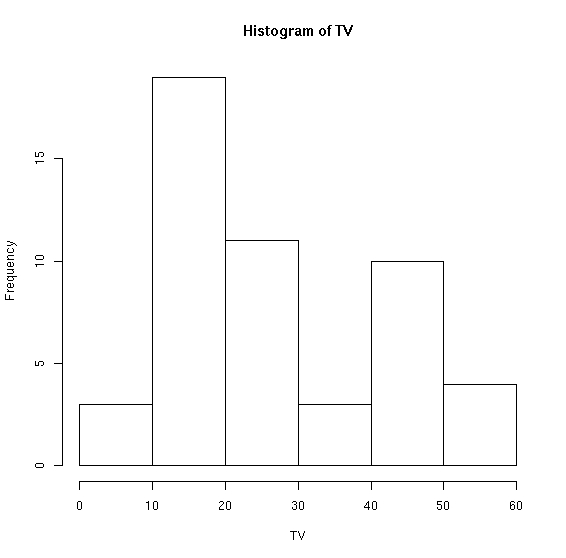
\includegraphics[width=0.5\textwidth]{imagenes/r_hist.eps}
%\caption{Histograma obtenido con {\tt hist (TV)}}
%\end{figure}

\begin{figure}[hbtp]
\centering
\subfigure[Gr�fico Q-Q para {\tt Lectura}]{%
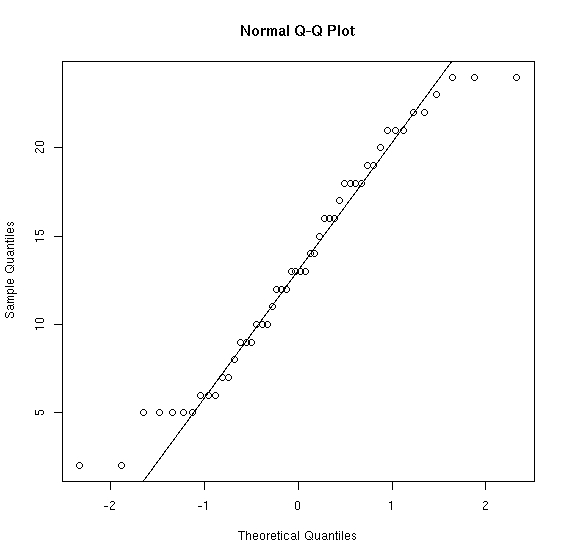
\includegraphics[width=0.49\textwidth]{imagenes/r_qqplot_1.eps}}
\subfigure[Gr�fico Q-Q para {\tt TV}]{%
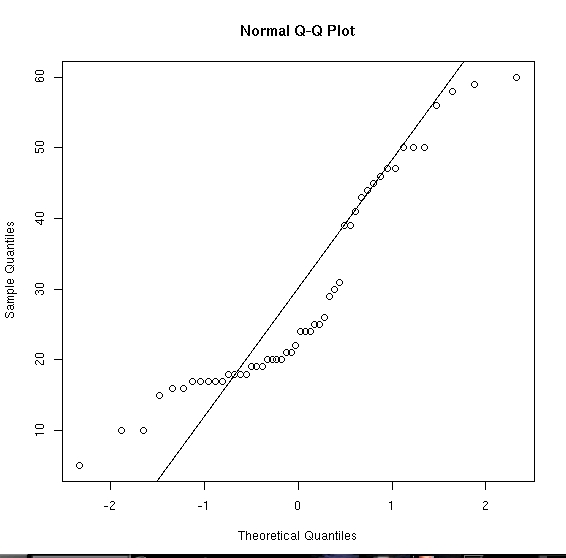
\includegraphics[width=0.49\textwidth]{imagenes/r_qqplot_2.eps}}
\caption{Gr�ficos Q-Q para dos variables, una que se comporta como una
normal y otra que no}
\end{figure}

% Esta figura  m�ltiple ocupar� toda una  p�gina, as� que no  la pongo
% antes que el histograma
\begin{figure}[p]
\centering
\subfigure[{\tt plot (Lectura)}]{%
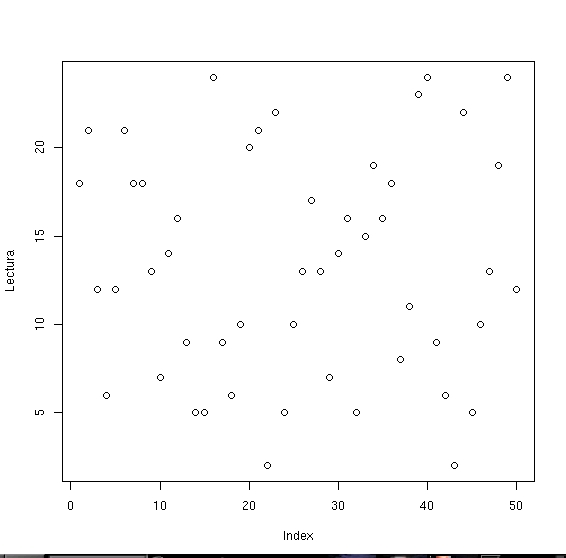
\includegraphics[width=0.49\textwidth]{imagenes/r_plot_1.eps}}
\subfigure[{\tt plot (Lectura, TV)}]{%
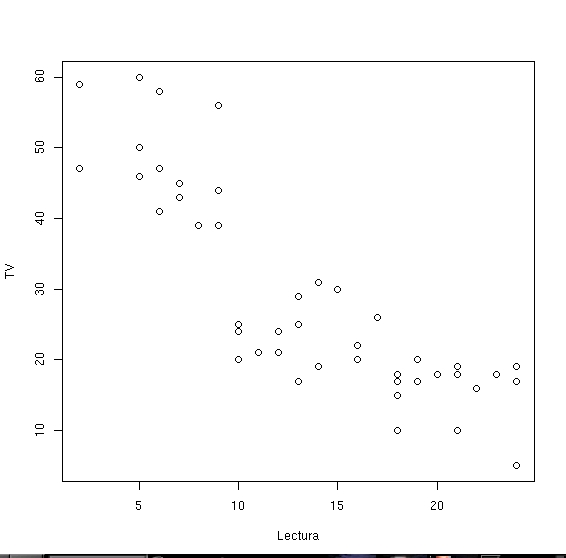
\includegraphics[width=0.49\textwidth]{imagenes/r_plot_2.eps}}
\subfigure[{\tt plot (Ingresos)}]{%
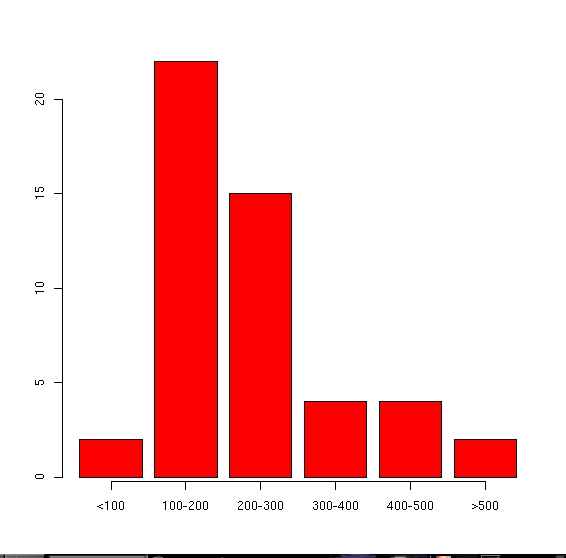
\includegraphics[width=0.49\textwidth]{imagenes/r_plot_3.eps}}
\subfigure[{\tt plot (Ingresos, Habitat)}]{%
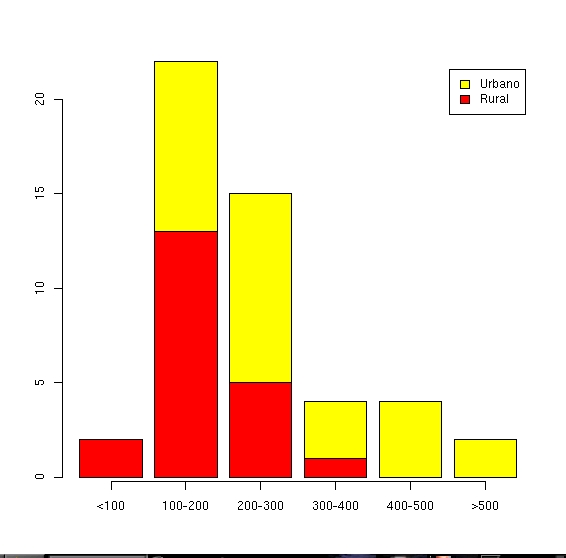
\includegraphics[width=0.49\textwidth]{imagenes/r_plot_4.eps}}
\caption{Las distintas formas de la funci�n {\tt plot()}}
\end{figure}

\index{R!gr�ficas!image@{\tt image()}}
\index{R!gr�ficas!contour@{\tt contour()}}
\index{R!gr�ficas!persp@{\tt persp()}}

Para  representar  matrices puedes  optar  por  ver sus  valores  como
im�genes. La  funci�n {\tt image()} lo  hace a modo de  una rejilla de
rect�ngulos de  diferentes colores  para representar  el valor  de las
celdas. Para  verlo en forma de  contorno usa {\tt contour()},  y para
verlo en perspectiva utiliza {\tt persp()}.

\begin{figure}[htbp]
\centering
\subfigure[{\tt image(volcano)}]{%
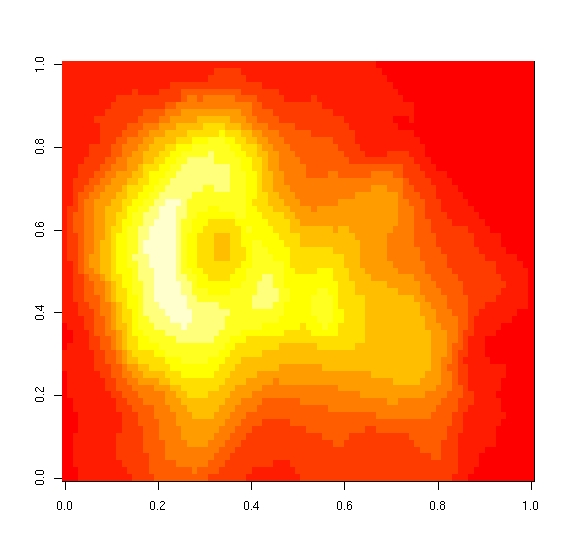
\includegraphics[width=0.3\textwidth]{imagenes/r_image.eps}}
\subfigure[{\tt contour(volcano)}]{%
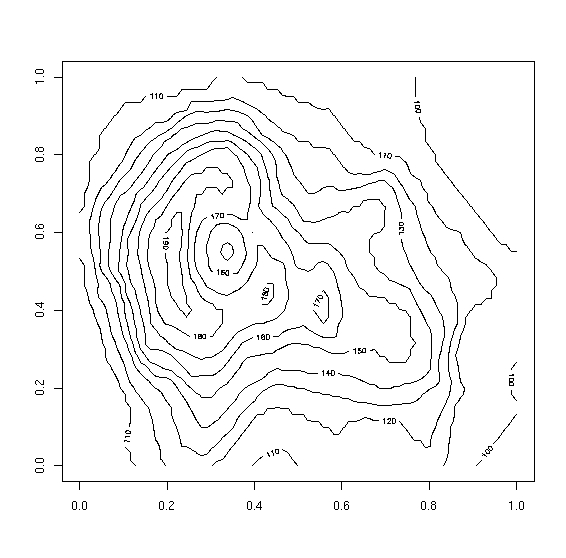
\includegraphics[width=0.3\textwidth]{imagenes/r_contour.eps}}
\subfigure[{\tt persp(volcano)}]{%
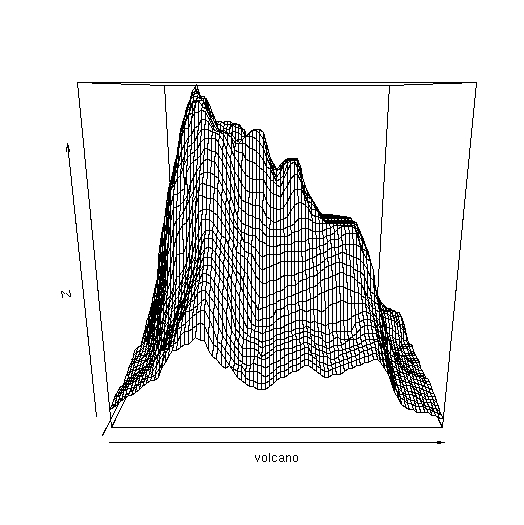
\includegraphics[width=0.3\textwidth]{imagenes/r_persp.eps}}
\caption{Gr�ficas para  representar matrices. El objeto  {\tt volcano}
lo obtenemos al ejecutar {\tt data(volcano)}}
\end{figure}

Los gr�ficos de sectores te dan una impresi�n clara a primera vista de
los  porcentajes que  tienen cada  ``clase'' en  una clasificaci�n  de
datos.  Por ejemplo  para ver  los porcentajes  de personas  seg�n las
edades representamos en un gr�fico de sectores el n�mero de individuos
que tiene cada edad. Una forma de hacerlo (seguramente no es la mejor)
ser�a:

\index{R!gr�ficas!de sectores}

\begin{verbatim}
> pie (tapply (Edad, fedad, length))
\end{verbatim}

\index{R!gr�ficas!pie@{\tt pie()}}

\begin{figure}[hbtp]
\centering
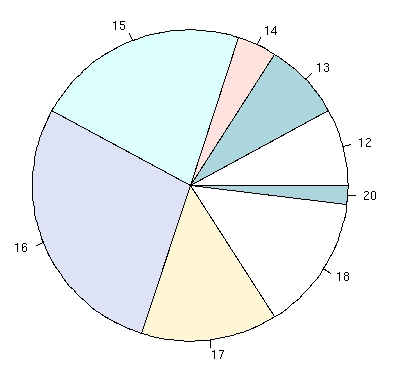
\includegraphics[width=0.7\textwidth]{imagenes/r_pie.eps}
\caption{Diagrama de sectores para la {\tt Edad}}
\end{figure}




\chapter{Yacas}

En  este tema  aprender�s a  utilizar el  programa Yacas  para relizar
c�lculos simb�licos.  Este tipo de  c�lculos resulta de  gran utilidad
puesto que  funciona de  la misma  forma que har�as  t� mismo  a mano,
operando con expresiones matem�ticas sin calcular el valor num�rico de
cada expresi�n. 

En  la  web  del proyecto  Yacas  ({\tt  http://yacas.sourceforge.net}
encontrar�s el  c�digo fuente  del programa  y toda  su documentaci�n:
desde  un tutorial  b�sico hasta  una gu�a  de programaci�n  en Yacas.

\section{�Qu� es Yacas?}

Yacas  es un  Sistema  de  �lgebra Computacional  (en  ingl�s CAS,  de
Computer  Algebra  System) de  prop�sito  general  f�cil de  usar.  Un
Sistema  de �lgebra  Computacional (SAC)  es un  programa que  permite
manipulaciones simb�licas sobre expresiones matem�ticas, reduciendo el
tiempo necesario  para realizar  c�lculos embarazosos  pero triviales.
Esto se hace  no mediante n�meros, sino mediante s�mbolos,  por lo que
el resultado de una operaci�n con expresiones matem�ticas es una nueva
expresi�n matem�tica.

Yacas  est�  construido  sobre  su  propio  lenguaje  de  programaci�n
dise�ado  para  este  prop�sito,  en  el  que  se  pueden  implementar
f�cilmente  nuevos  algoritmos.  Adem�s, incorpora  una  documentaci�n
extensa sobre las funcionalidades que  implementa y los m�todos usados
para implementarlas.

Entre las caracter�sticas que  Yacas implementan encontramos precisi�n
arbitraria, n�meros racionales,  vectores, n�meros complejos, c�lculos
con  matrices  (incluyendo  inversas, determinantes  y  resoluci�n  de
sistemas lineales), derivaci�n, series  de Taylor, resoluci�n num�rica
(m�todo  de Newton),  y un  mont�n m�s  de algoritmos  no matem�ticos.
Tiene  tambi�n  soporte  b�sico   para  polinomios  en  una  variable,
integraci�n de funciones y c�lculo tensorial.

\section{Empezando con Yacas}

Yacas  tiene  un  int�rprete  de comandos  que  nos  permite  ejecutar
funciones para probar  lo que queremos programar,  para luego escribir
un script.  Para entrar al int�rprete  de Yacas basta con  ejecutar el
comando  {\tt  yacas}  en  una  consola o  terminal.  Para  salir  del
int�rprete puedes  pulsar {\tt Control-C}  o bien ejecutar  la funci�n
\verb+quit();+.

\begin{verbatim}
$ yacas
[editvi.ys] [unix.ys] 
True;
Numeric mode: "Gmp"
To exit Yacas, enter  Exit(); or quit or Ctrl-c. Type ?? for help.
Or type ?function for help on a function.
Type 'restart' to restart Yacas.
To see example commands, keep typing Example();
In>
\end{verbatim}

Tambi�n   existe  una   interfaz  gr�fica   llamada  Porteus.   Si  la
tienes  instalada  deber�as  poder  iniciarla  ejecutando  el  comando
\verb+proteusworksheet+. Esta  utilidad te  proporcioa un  entorno m�s
c�modo e integrado  en el que puedes probar c�digo  en el int�rprete e
ir escribiendo un script en el editor que incluye.

\begin{figure}[htbp]
\centering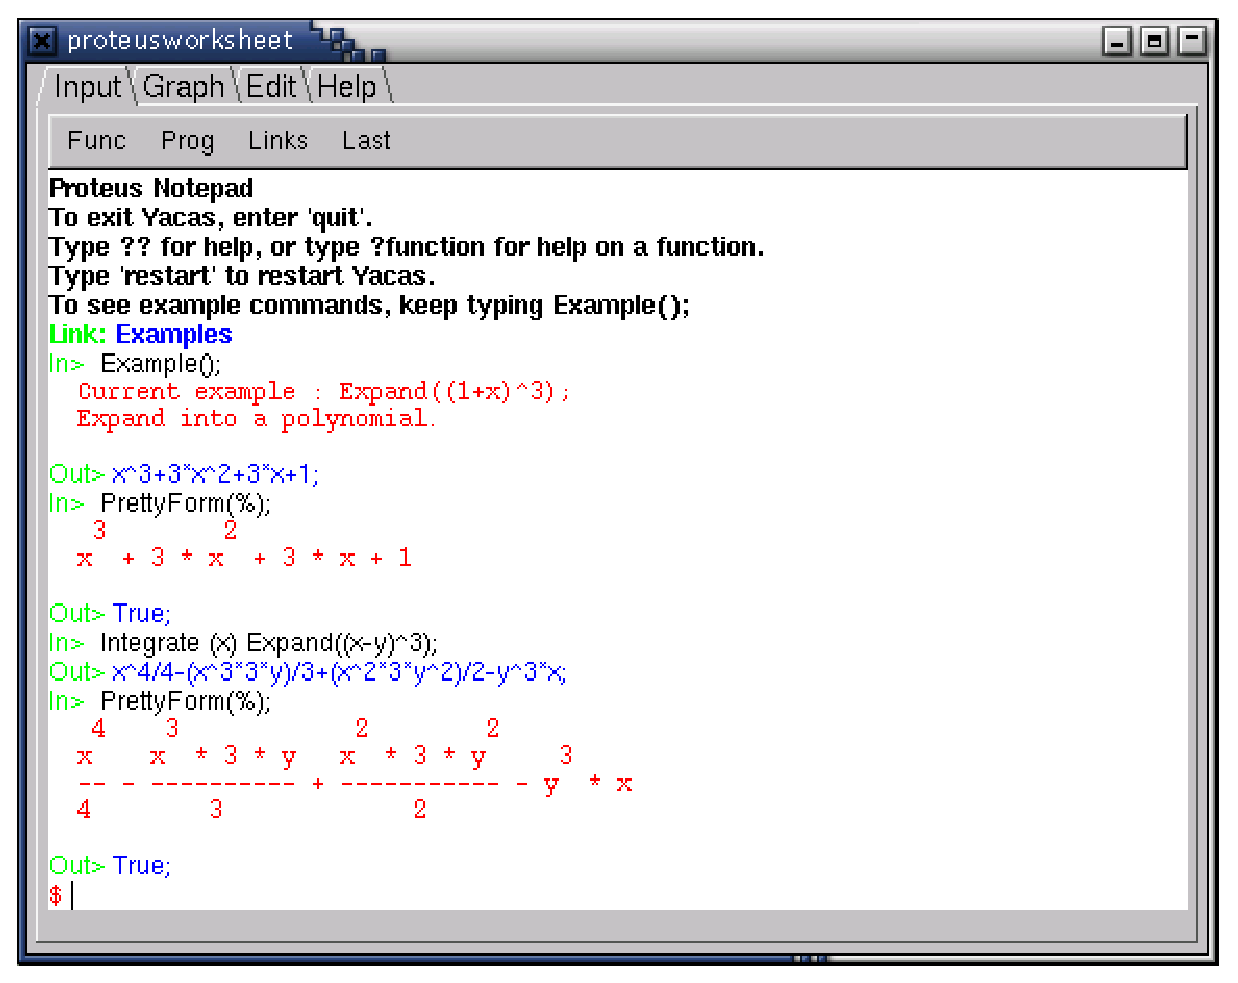
\includegraphics[width=0.7\textwidth]{imagenes/proteus.eps}
\caption{Proteus, interfaz gr�fica para Yacas}
\end{figure}

La �ltima l�nea (\verb+In>+) es el prompt de entrada de Yacas, que nos
indica que  el int�rprete est�  esperando nuestras �rdenes.  Todas las
�rdenes de Yacas deben terminar con un punto y coma (\verb+;+), aunque
el int�rprete suele  a�adirlo si no lo ponemos. Sin  embargo a la hora
de programar en  Yacas veremos que el punto y  coma hay que escribirlo
siempre,  de modo  que es  mejor acostumbrarse  a ponerlo  para evitar
posteriores dolores de cabeza.

Para ir abriendo  el apetito sigue la sugerencia de  Yacas: ejecuta la
funci�n  \verb+Ejample();+ varias  veces. Por  supuesto no  tienes que
teclear el comando todas las veces, ya que Yacas cuenta con edici�n de
l�nea al estilo de GNU Emacs (utiliza GNU readline). Esto quiere decir
que todos  los comandos  que ejecutes  en Yacas  se almacenar�n  en un
historial, y para repetirlos puedes  recuperarlos pulsando la tecla de
cursor  hacia arriba.  Este  historial queda  guardado  en el  fichero
\verb+.yacas_history+ en tu directorio  personal. Veamos la salida que
produce Yacas tras varias ejecuciones de \verb+Ejample();+

\begin{verbatim}
In> Example();
Current example : 40!;

Simple factorial of a number.

Out> 815915283247897734345611269596115894272000000000;
In> Example();
Current example : D(x)Sin(x);

Taking the derivative of a function (the derivative of Sin(x) with
respect to x in this case).

Out> Cos(x);
In> Example();
Current example : Taylor(x,0,5)Sin(x);

Expanding a function into a taylor series.

Out> x-x^3/6+x^5/120;
In> Example();
Current example : Integrate(x,a,b)Sin(x);

Integrate a function.

Out> Cos(a)-Cos(b);
In> Example();
Current example : Solve(a+x*y==z,x);

Solve a function for a variable.

Out> (z-a)/y;
In> Example();
Current example : Limit(x,0)Sin(x)/x;

Take a limit.

Out> 1;
\end{verbatim}

En cualquier momento puedes acceder  a la documentaci�n de una funci�n
ejecutando la funci�n  precedida por un signo  de interrogaci�n, p.ej.
\verb+?IsFreeOf+. Un detalle  importante de Yacas es  que, como muchos
lenguajes del mundo de Un*x, es sensible a las may�sculas; esto es, no
es lo mismo \verb+esto+ que \verb+Esto+ ni que \verb+eSTO+.

Estos ejemplos ilustran  lo f�cil que es obtener  buenos resultados en
c�lculos  simb�licos  con  Yacas.  Sin embargo  es  probable  que  los
resultados  de  los siguientes  ejemplos  no  te resulten  f�ciles  de
interpretar:

\begin{verbatim}
In> Integrate(x) ((x-y)^3)
Out> x^4/4-(x^3*3*y)/3+(x^2*3*y^2)/2-y^3*x;
\end{verbatim}

la forma en  que Yacas recibe nuestra orden de  integrar $\int (x-y)^3
\, dx$ no es nada cr�ptica, pero su respuesta no es precisamente f�cil
de  leer. Esta  forma de  mostrar  las expresiones  matem�ticas es  la
normal  en  Yacas,  pero  no  la �nica.  Podemos  pedir  a  Yacas  que
muestre  las  expresiones  de  forma m�s  ``bonita''  con  la  funci�n
\verb+PrettyForm()+.

\begin{verbatim}
In> PrettyForm(%)

 4    3            2        2         
x    x  * 3 * y   x  * 3 * y     3    
-- - ---------- + ----------- - y  * x
4        3             2              

Out> True;
\end{verbatim}

El signo  \verb+%+ es una referencia  que se apunta siempre  al �ltimo
valor  devuelto por  el  int�rprete, es  decir lo  que  aparezca a  la
derecha del  �ltimo \verb+Out>+. Esta referencia  s�lo est� disponible
cuando usamos Yacas como int�rprete  interactivo, no se puede utilizar
desde un script.

Otras  formas  de mostrar  una  expresi�n  son  las utilizadas  en  el
lenguaje  de  programaci�n  C  y  en  el  lenguaje  tipogr�fico  \TeX.
Para  mostrar  una  expresi�n  de estas  formas  est�n  las  funciones
\verb+CForm()+  y \verb+TeXForm()+  respectivamente. F�jate  que estas
funciones  no devuelven  la  expresi�n  que muestran,  por  lo que  no
podemos  utilizar  la  referencia  \verb+%+ dos  veces  seguidas  para
mostrar  una  expresi�n  (la  segunda mostrar�a  la  expresi�n  l�gica
\verb+True+). Por  eso escribimos  \verb+Integrate(x) ((x-y)^3)+
en cada l�nea:

\begin{verbatim}
In> CForm (Integrate(x) ((x-y)^3))
Out> "pow(x, 4.) / 4. - ( pow(x, 3.) * 3. * y)  / 3. + ( pow(x, 2.) * 
3. * pow(y, 2.))  / 2. - pow(y, 3.) * x";
In> TeXForm (Integrate(x) ((x-y)^3))
Out> "$\frac{x ^{4}}{4}  - \frac{x ^{3} 3 y}{3}  + \frac{x ^{2} 3 y ^{
2}}{2} - y ^{3} x$";
\end{verbatim}

La funci�n \verb+CForm()+ devuelve la expresi�n escrita en lenguaje C,
de forma que  podemos incluirla en el  c�digo de un programa  en C. La
funci�n \verb+TeXForm()+ devuelve la  expresi�n escrita en el lenguaje
tipogr�fico  \TeX, de  forma  que podemos  incluirla  en un  documento
escrito en  \TeX~ o \LaTeX.  Por ejemplo,  este libro est�  escrito el
\LaTeX, lo  que me  permite incluir la  salida de  \verb+TeXForm()+ en
este  mismo p�rrafo  con  s�lo copiar  y pegar.  De  esta forma  puedo
escribir $\int (x-y)^3 \, dx = \frac{x ^{4}}{4} - \frac{x ^{3} 3 y}{3}
+ \frac{x ^{2} 3 y ^{2}}{2} - y ^{3} x$.

En ocasiones nos  interesa conocer el valor num�rico  de una expresi�n
determinada, y posiblemente s�lo nos interese un n�mero determinado de
decimales.  Yacas  es un  lenguaje  de  precisi�n arbitraria,  lo  que
significa que puedes  pedirle toda la precisi�n que  quieras, pero ten
cuidado no le pidas demasiada precisi�n  si tu m�quina no es realmente
potente.

La funci�n \verb+Precision()+ establece  el n�mero de cifras decimales
con  las  que se  aproximar�n  los  valores. Estas  aproximaciones  se
realizan con  la funci�n  \verb+N()+, que  adem�s permite  saltarse la
precisi�n establecida por \verb+Precision()+ pas�ndosela como segundo
par�metro. En el siguiente ejemplo se ilustra esto:

\begin{verbatim}
In> alpha := Sqrt (Pi ())
Out> Sqrt(3.1415926535897932384626433832795028841971694);
In> Precision (2);
Out> True;
In> N (alpha)
Out> 1.77;
In> Precision (20);
Out> True;
In> N (alpha)
Out> 1.77245385090551602729;
In> N (alpha, 50)
Out> 1.77245385090551602729816748334114518279754945629866;
\end{verbatim}

Normalmente  no hay  problema  por  pedirle a  Yacas  unos cientos  de
d�gitos de precisi�n, pero siempre que  vayas a trabajar con n�meros o
precisiones enormes recuerda que el tiempo necesario para los c�lculos
aumentar� r�pidamente.

\section{Variables}

En Yacas se entiende por variable un objeto al que se puede asignar un
valor.  Las variables  pueden  llamarse como  quieras  siempre que  el
nombre  empiece  por  una  letra  y contin�e  con  letras  y  n�meros.
Para  asignar un  valor  a  una variable  se  utiliza  el operador  de
asignaci�n \verb+:=+ en lugar de \verb+=+ (este �ltimo se utiliza como
comparador). En cualquier momento puedes  ver el valor de una variable
tecleando su nombre como si fuera  un comando de Yacas, y esto tambi�n
es v�lido en un script. Asignaciones v�lidas son:

\begin{verbatim}
In> n := 10;
Out> 10;
In> m := n!;
Out> 3628800;
In> n
Out> 10;
In> m
Out> 3628800;
\end{verbatim}

Si en alg�n momento quieres que una variable pierda su valor no tienes
m�s que ``limpiarla'' con la funci�n \verb+Clear()+:

\begin{verbatim}
In> m
Out> 3628800;
In> Clear (m);
Out> True;
In> m
Out> m;
\end{verbatim}

\section{Funciones}

Las funciones  son como las  variables, con  el a�adido de  que pueden
depender de una o m�s  variables. Adem�s con Yacas podemos sobrecargar
una funci�n, esto  es, definir dos funciones con el  mismo nombre pero
distinto n�mero de  variables de forma que se eval�e  una u otra seg�n
el n�mero de par�metros que reciba.

Como ejemplo definimos la funci�n \verb+Area+ de dos formas: si recibe
un par�metro  devuelve el �rea  del c�rculo con  el radio igual  a ese
par�metro, pero si recibe dos par�metros devuelve el �rea de la elipse
que tenga esos dos par�metros como radios.

\begin{verbatim}
In> Area (r) := Pi () * r^2;
Out> True;
In> Area (a, b) := Pi () * a * b;
Out> True;
In> Area (3);
Out> 28.2743338823;
In> Area (3, 5);
Out> 47.1238898035;
\end{verbatim}

Cuando  definimos una  funci�n en  Yacas, la  parte a  la derecha  del
operador de asignaci�n \verb+:=+ no se  eval�a sino que se asigna como
expresi�n a la  funci�n. Si quieres que Yacas eval�e  la parte derecha
de  la  definici�n de  una  funci�n  puedes  forzarlo con  la  funci�n
\verb+Eval()+. Esto es  �til cuando la evaluaci�n de  la parte derecha
resulta computacionalemente costosa, por ejemplo  en el caso de series
de Taylor.  Si evaluamos una  expansi�n en  series de Taylor  antes de
asignarla a la funci�n, la m�quina no tendr� que calcular la expansi�n
cada vez que la funci�n sea llamada.

\begin{verbatim}
In> f(x) := Eval (Taylor (x, 0, 9) Sin(x))
Out> True;
In> f(x)
Out> x-x^3/6+x^5/120-x^7/5040+x^9/362880;
\end{verbatim}

\section{Listas}

Uno de  los elementos m�s  importantes del  lenguaje de Yacas  son las
listas, que como era de esperar son grupos de objetos ordenados. Yacas
representa las listas  con sus elementos entre llaves  y separados por
comas.  Los  vectores  son  listas,  y  las  matrices  son  listas  de
listas. De  hecho, cualquier expresi�n  matem�tica en Yacas  puede ser
transformada en una  lista. Para acceder a los elementos  de una lista
puedes  usar la  notaci�n habitual  en los  corchetes, y  no s�lo  con
n�meros sino tambi�n con secuencias de ellos.

\begin{verbatim}
In> lista := {a, b, c, d, e, f};
Out> {a,b,c,d,e,f};
In> lista[2];
Out> b;
In> lista[2 .. 4];
Out> {b,c,d};
\end{verbatim}

F�jate  que los  espacios a  ambos  lados del  operador \verb+..+  son
necesarios  para distinguir  estos puntos  de los  que podr�an  formar
parte de un n�mero.

Tambi�n puedes  indexar una lista  con palabras, no s�lo  con n�meros,
mientras que  los elementos de la  lista pueden ser cualquier  tipo de
objetos. Esto  te permite tener  peque�as bases  de datos en  forma de
listas asociativas con parejas clave -- valor.

\begin{verbatim}
In> pers := {};
Out> {};
In> pers["nombre"] := "Eric";
Out> True;
In> pers["apellido"] := "Cartman";
Out> True;
In> pers["edad"] := 7.34;
Out> True;
In> pers["educado"] := False;
Out> True;
In> pers
Out> {{"educado",False},{"edad",7.34},{"apellido","Cartman"},{"nombre","Eric"}};
\end{verbatim}

\section{Programando con Yacas}

\section{Gr�ficas con Yacas y GNUplot}

Yacas  incorpora la  posibilidad  de  representar gr�ficas  utilizando
GNUplot,  si  bien esta  capacidad  depende  de que  tengas  instalado
tambi�n el programa  GNUplot. La funci�n para  representar gr�ficas es
\verb+GnuPlot()+ y  recibe cuatro  par�metros: el  valor m�nimo  de la
variable,  el  valor  m�ximo  de  la variable,  el  n�mero  de  puntos
utilizados para la representaci�n y la funci�n para representar. En el
siguiente  ejemplo  calculamos  el polinomio  interpolador  de  cuatro
puntos y  lo representamos junto  a la funci�n $f(x)  = 2 \cdot  e^x -
x^2$.

\begin{verbatim}
In> f(x) := 2 * Exp(x) - x^2;
Out> True;
In> xlist := {0.0, 1.0, 1.5, 2.25};
Out> {0.0,1.0,1.5,2.25};
In> ylist := {2.0, 4.4366, 6.7134, 13.9130};
Out> {2.0,4.4366,6.7134,13.9130};
In> p (x) := LagrangeInterpolant (xlist, ylist, x);
Out> True;
In> GnuPlot(0, 3, 100, {f(x), p(x)})
GnuPlot: created file gnuplot.tmp/gnudata.in1
GnuPlot: created file gnuplot.tmp/gnudata.in2
Out> True;
\end{verbatim}

\begin{figure}[htbp]
\centering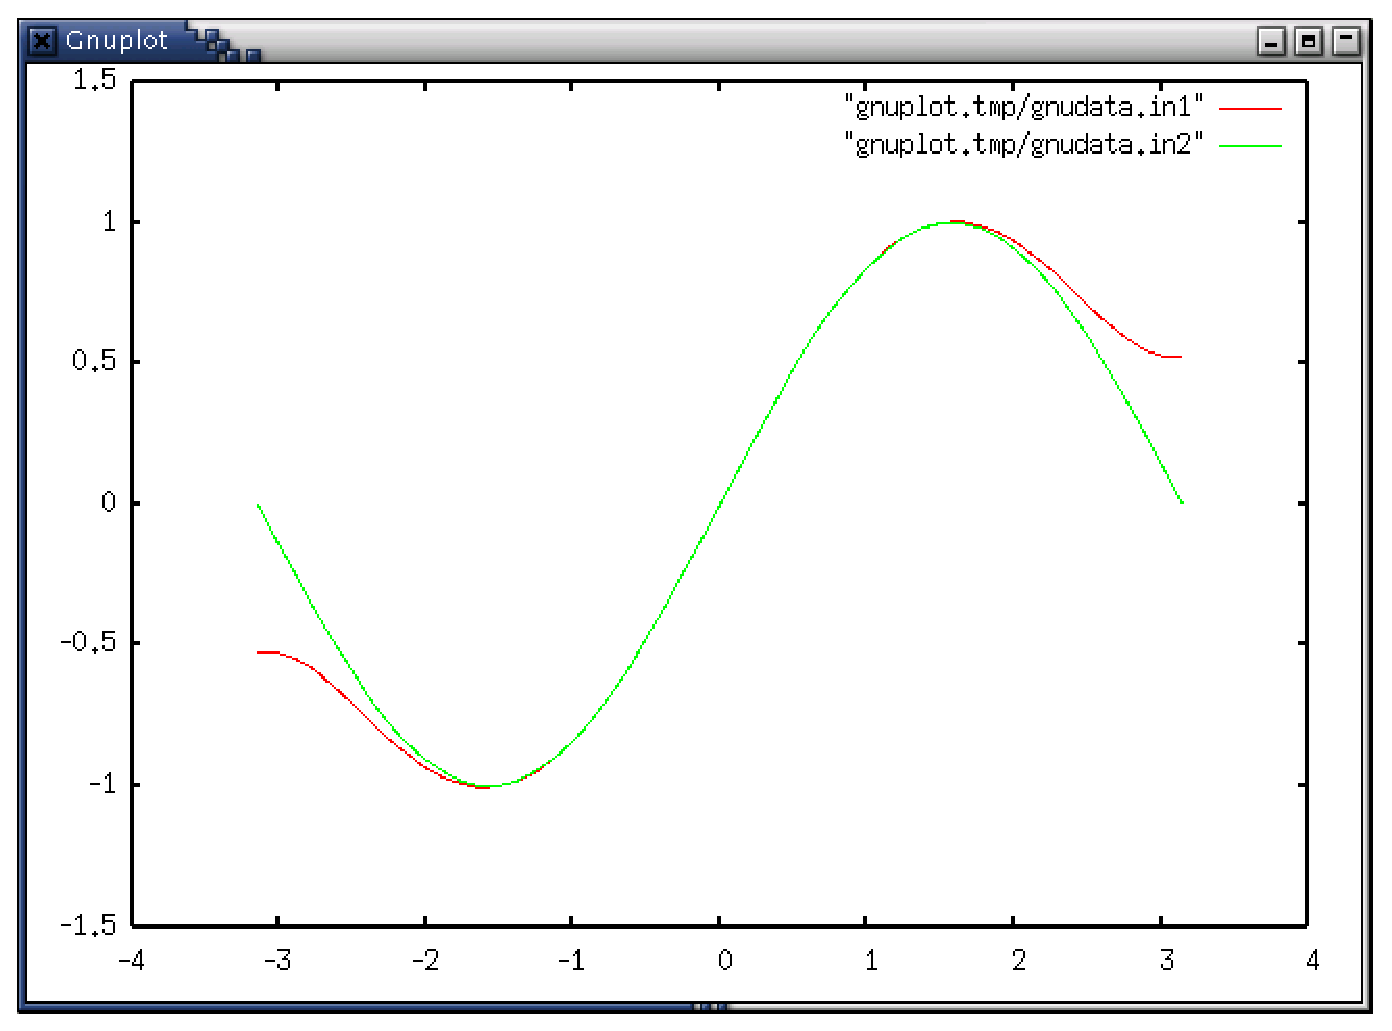
\includegraphics[width=0.7\textwidth]{imagenes/yacas_gnuplot.eps}
\caption{Representaci�n gr�fica con GNUplot desde Yacas}
\end{figure}



\section{Rizando el rizo}

\begin{verbatim}
In> f(x) := x^5;
Out> True;
In> f1(x) := D(x) f(x)
Out> True;
In> Eval (Subst(x, 1) f(x))
Out> 1;
In> Eval (Subst(x, 1) f1(x))
Out> 5;
\end{verbatim}



\chapter{Maxima}


% M�dulo V:   Programaci�n
% 1. Editores de texto (gvim, xemacs)
% 2. Bash
% 3. GNU Fortran 77
% 4. FreePascal
% 5. GNU C/C++
% 6. Java
% 7. GNU Make
% 8. Depuradores (gdb y ddd)
\part{Programaci�n}
%Autor: miguev && Carlos de la Cruz (frodo@fmat.ull.es)


\chapter{Editores de VI y Emacs}



\section{Joe}


El primer editor  que suele aprenderse en Linux es  {\tt Joe}, por ser
muy sencillo  y r�pido.  Puede usarse  para editar  cualquier fichero,
pero  aqu�  trataremos su  uso  b�sico  para editar  peque�os  textos,
ficheros de  configuraci�n, peque�os  programas. Todos  estos ficheros
pueden editarse con m�s comodidad con editores m�s potentes como Emacs
o VIM pero para ello es  necesario aprender a usarlos primero, lo cual
puede no resultar tan sencillo como aprender {\tt Joe}.

Veremos s�lo un par de comandos  de {\tt Joe}, simplemente como editar
un fichero existente o nuevo, guardarlo sin salir, salir sin guardarlo
y salir guard�ndolo. Para obtener m�s informaci�n sobre otras opciones
del editor existe el comando de ayuda que explicaremos luego.

El  manejo de  {\tt Joe}  se basa  en combinaciones  de teclas  con la
tecla {\tt  Control}. Denotaremos  por {\tt  \flq Ctrl\frq  x y}  a la
combinaci�n de teclas que se obtiene al pulsar la tecla {\tt Control},
seguidamente (sin soltar la primera) pulsar la tecla {\tt x} y despu�s
(soltando las  teclas anteriores) pulsar  la tecla {\tt y}.  Veamos un
r�pido ejemplo del uso de este editor. En un terminal ejecutamos:

\begin{verbatim}
$ joe prueba.txt
\end{verbatim}


Escribimos una frase sencilla, tal como:


\begin{verbatim}
Si algo funciona, no lo toques.
\end{verbatim}

Para guardar el fichero utilizamos la combinaci�n de teclas {\tt \flq
Ctrl\frq k s} y entonces {\tt Joe} nos preguntar� el nombre con el que
queremos guardar el fichero.

\begin{verbatim}
Name of file to save (^C to abort): hola.txt
\end{verbatim}

Si pulsamos ahora  ahora {\tt \flq Ctrl\frq  c} simplemente cancelamos
la orden  de guardar el fichero,  pero no perdemos su  contenido. Para
guardar el  fichero pulsamos  {\tt Enter},  modificando el  nombre del
fichero si lo deseamos. Ahora a�adimos otra l�nea:

\begin{verbatim}
Si algo funciona, no lo toques.
Si algo funciona, y no sabes por qu�, �salo siempre.
\end{verbatim}

Ahora saldremos  del editor {\bf  guardando los cambios},  mediante la
combinaci�n  de  teclas  {\tt  \flq  Ctrl\frq k  x}.  De  esta  manera
volveremos al prompt  del sistema siendo informados de  que el fichero
ha sido guardado.

\begin{verbatim}
File prueba.txt saved.
$
\end{verbatim}

Como �ltima maniobra, abrimos de  nuevo el fichero, borramos la �ltima
l�nea y salimos sin guardar los cambios.


\begin{verbatim}
$ joe prueba.txt
\end{verbatim}

Boramos la �ltima l�nea como har�amos  en el {\tt edit} del {\tt DOS},
y pulsamos {\tt  \flq Ctrl\frq c} para salir sin  guardar los cambios.
El editor  nos pedir� confirmaci�n  antes de salir.  Podemos responder
que s� queremos salir pulsando {\tt y}, o por el contrario cancelar la
maniobra pulsando  {\tt n}  o {\tt  \flq Ctrl\frq  c}. Decimos  que s�
({\tt y}) y volvemos al prompt del sistema.

\begin{verbatim}
Lose changes to this file (y,n,^C)? 
File hola.txt not saved.
$
\end{verbatim}

Esto es lo m�nimo  que debemos saber para editar con  {\tt Joe}, y con
esto nos conformaremos  aqu� pues en lo sucesivo  aprenderemos a hacer
operaciones m�s avanzadas con otros editores. Para conocer sobre otras
opciones  de  este editor,  se  puede  utilizar  la opci�n  {\tt  \flq
Ctrl\frq k h}.

      

\section{Emacs }


{\tt Emacs}, junto con {\tt VI},  ha sido uno de los primeros editores
de  texto para  UNIX. A  pesar  de visualmente  presentar un  interfaz
similar al  de un  editor de  texto corriernte,  como podr�a  ser {\tt
joe},  el {\tt  edit} de  MS-DOS, o  similar, lo  cierto es  que tiene
much�simas posibilidades que uno no atribuir�a a un editor de texto en
modo consola. Por  ejemplo, el indentado autom�tico  de c�digo Pascal,
Java, C, o cualquier lenguaje para  el que haya escrito un m�dulo para
Emacs de  asistencia a  la programaci�n,  nos ofrece  posibilidades de
trabajar con  CVS, enviar correo  electr�nico, y un largo  etc�tera de
posibilidades. Como an�cdota cabe contar,  para que se hagan una idea,
el manual de GNU Emacs, en formato ASCII ocupa cerca de 1.1 MB.


Hablemos de c�mo manejarse con los  men�s de Emacs. Existen cientos de
combinaciones de teclas en Emacs que nos permiten hacer cualquier cosa
sin  ver  un  men�.  Los  usuarios  expertos  de  Emacs  valoran  esta
posibilidad, pues a la hora de  escribir con prisas, un men� puede ser
algo muy inc�modo.  Pero para ustedes que  est�n empezando, recuerden:
la tecla {\tt \flq F10\frq } es su amiga.

La tecla {\tt \flq F10\frq } nos da acceso a todos los men�s de Emacs,
menu archivo, edici�n, cambio entre  las distintas ventanas de edici�n
de texto, etc.

Empezemos viendo como editar un fichero de texto b�sico. En la consola
ponemos:

\begin{verbatim}
$ emacs prueba.c
\end{verbatim}

y escribimos un programa com�n y corto:

\begin{verbatim}
#include <stdio.h>
int
main()
{
  printf("\nHola Mundo\n\n");
}
\end{verbatim}

Como podemos apreciar,  Emacs hace retroceder el cursor  al cerrar los
corchetes y los par�ntesis, para  indicarnos d�nde los abrimos y tener
una  referencia de  cu�les quedan  a�n  por cerrar.  Probemos ahora  a
guardar  nuestro peque�o  programa  C. Para  ello  pulsamos {\tt  \flq
F10\frq }  y una vez  pulsada {\tt \flq F10\frq  } vemos que  la tecla
{\tt B} nos dar�a acceso al men� buffers (que no son otra cosa que las
distintas ventanas que tenemos abiertas),  la {\tt F} nos dar�a acceso
al men� {\tt  files} (el cual hace pr�cticamente lo  mismo que el men�
archivo de  cualquier editor de texto,  etc... y la tecla  {\tt C} nos
dar�a  acceso, si  las  tenemos instaladas,  a  las posibilidades  que
ofrece  emacs para  la  edici�n de  c�digo en  C.  Como s�lo  queremos
guardar,  pulsamos despu�s  de {\tt  \flq F10\frq  }, {\tt  S}. Ya  lo
tendr�amos guardado.  Otra cosa muy importante,  en cualquier programa
es saber  salir. Esto se  hace con  {\tt \flq F10\frq  }, {\tt F}  y a
continuaci�n la tecla {\tt S}. Nos  pregunta, si no lo hemos hecho ya,
que  si deseamos  guardar. Escribimos  {\tt yes}  (hay que  escribirlo
entero)  o  {\tt no},  y  a  continuaci�n  nos pregunta  si  realmente
queremos salir,  a lo cual ahora  s�, responderemos {\tt y}  para {\tt
s�} o {\tt n} para {\tt no}.


Desplaz�ndonos por el texto:

Emacs es famoso por sus innumerables combinaciones de teclas para realizar
cualquiera de las operaciones que nos ofrece. Algunas de las combinaciones
de teclas para movernos c�modamente por nuestros documentos son:
\begin{verbatim}

Alt + f : Sit�a el cursor al principio de la palabra siguiente.
Alt + b : Sit�a el cursor al principio de la palabra anterior.
Ctrl + a : Sit�a el cursor al principio de la l�nea actual.
Ctrl + e : Sit�a el cursor al final de la l�nea actual.
Alt + a : Retrocede el cursor hasta el principio de la frase.
Alt + e : Avanza el cursor hasta el final de la frase.
Home(Inicio): Nos permite situarnos al principio del "buffer".
End(Fin): Nos permite situarnos al final del "buffer".
Ctrl + l: Sit�a el cursor justo al principio de la l�nea del medio de la
	  pantalla

\end{verbatim}

Algunas teclas para eliminar texto:

\begin{verbatim}

Alt + d : Elimina la palabra que sigue al cursor.
Alt + delete(supr) : Elimina la palabra anterior al cursor.
Ctrl + k : Elimina la l�nea actual entera.
Alt + k : Elimina la frase siguiente
Ctrl x + BackSpace : Elimina la frase anterior

\end{verbatim}





Hay que a�adir un truco bastante �til que es la combinaci�n de teclas
Ctrl + u, la cual nos permite repetir cualquier comando n veces.

Por ejemplo, si quisi�ramos avanzar 24 palabras, utilizar�amos la secuencia
de teclas:

"Ctrl U" "24" "Alt + f"



Otra funci�n  muy b�sica tambi�n  es la  de buscar y  reemplazar texto.
Esto puede hacerse  c�modamente con la combinaci�n  {\tt \flq Ctrl\frq
-s}, dejando  pulsado la  tecla {\tt \flq  Control}\frq y  pulsando la
{\tt s}, y a continuaci�n poniendo que queremos buscar y pulsando {\tt
Enter}.  Una  vez  encuentre  la primera  coin\-ci\-den\-cia,   puede
seguir busc�ndose el  mismo patr�n  pulsando de  nuevo simplemente  {\tt \flq
Ctrl\frq -s}.

Podemos saber  en todo momento  qu� estamos haciendo fij�ndonos  en la
l�nea inferior de la pantalla de Emacs.

Para  reemplazar  trozos  de  texto, cosa  tambi�n  de  supervivencia,
podemos hacerlo f�cilmente de la siguiente forma:

\begin{enumerate}
\item Pulsamos \flq F10\frq .
\item Pulsamos la S, que corresponde al men� Search.
\item Nos sale el siguiente men�:
\end{enumerate}

\begin{verbatim}
Possible completions are:
S==\frq Search...                      R==\frq Regexp Search...
B==\frq Search Backwards...            0==\frq Regexp Search Backwards...
1==\frq Repeat Search                  2==\frq Repeat Regexp
3==\frq Repeat Backwards               4==\frq Repeat Regexp Backwards
5==\frq Bookmarks                      F==\frq Find Tag...  (M-.)
Q==\frq Query Replace...  (M-%)        6==\frq Query Replace Regexp...
\end{verbatim}

Pulsamos {\tt Q} y nos dice:

{\tt Query  replace:} donde escribiremos  lo que queremos  buscar para
ser reemplazado, y pulsamos {\tt Enter}.

Luego,  emacs  nos   pregunta:  {\tt  query  replace   with:  }  donde
escribiremos el  texto con  el cual  queremos sustituir,  y pulsaremos
enter.

En este  men�, encontramos  tambi�n una serie  de comandos,  como {\tt
query  regexp},  {\tt  query  replace regexp},  etc.,  que  aunque  no
entraremos en ellos,  son muy interesantes, pues  nos permiten buscar,
no  ya patrones  de  texto concretos,  sino un  tipo  de b�squeda  m�s
avanzada por  medio de  expresiones regulares (regular  expressions en
ingl�s), esto es,  ``todas las palabras que empiecen por  c y terminen
por j''  o ``todas  las may�sculas cambiarlas  por min�sculas''  en el
caso de {\tt query replace regexp}.

Insertando un fichero de texto en nuestro documento:

Para los amantes del Cut & Pasting (un deporte muy extendido en algunos
c�rculos de programadores), aqu� va un comando que nos permite introducir
un documento de texto dentro de otro:

Pulsamos las teclas "Ctrl x", seguidas de la letra "i", para insertar un
fichero en la posici�n actual del cursor. Entonces, en la l�nea de comandos
de emacs, aparecer� el directorio actual. 

Escribimos la ruta completa al archivo y aparecer� en la posici�n actual
del cursor.




\section{VI y VIM}


{\tt VI} es un editor de texto visual, de pantalla completa, basado en
el editor de  l�nea {\tt ex}. Es  un editor poco intuitivo  y con mala
prensa entre los estudiantes que dan sus primeros pasos en UNIX/Linux,
pero por otra parte es el  editor favorito de los usuarios avanzados y
de muchos programadores. Es adem�s un editor que se puede encontrar en
cualquier sistema UNIX, desde antiguas  estaciones Sun Solaris o HP-UX
hasta  las  m�s  recientes  distribuciones  de  GNU/Linux  o  FreeBSD,
OpenBSD, etc.  {\tt VI} es adem�s  un editor muy potente,  que permite
hacer  complicadas  operaciones en  grandes  ficheros  con unos  pocos
comandos, por  lo que  su aprendizaje  puede ahorrarnos  mucho tiempo.
Otra ventaja de {\tt VI} es que al ser tan corriente suele encontrarse
incluso en disquetes de rescate. L�gicamente poco se puede rescatar si
no  se sabe  manejar  el  �nico editor  disponible  en  un momento  de
emergencia. Pero  el manejo de {\tt  VI} es realmente inc�modo  si nos
enfrentamos  a la  versi�n cl�sica.  Por ejemplo  no podemos  usar los
cursores  para  movernos  por  el  texto,  debemos  pasar  al  llamado
``modo comando'' y utilizar letras para movernos.

En este  curso utilizaremos el  editor {\tt VIM}. {\tt  VIM} significa
``{\bf V}i {\bf IM}proved''  (``{\bf VI M}ejorado''), y como
su nombre  indica es un  clon (muy)  mejorado del cl�sico  editor {\tt
VI}. {\tt VIM}  es bastante m�s amigable que {\tt  VI}, ya que permite
un uso m�s intuitivo (p.ej. los cursores y otras teclas para moverse).


Lo primero  que debe aprenderse con  {\tt VIM} es la  filosof�a de los
dos modos de  trabajo: el modo {\tt comando} y  el modo {\tt edici�n}.
El  modo comando  se utiliza  s�lamente  para dar  �rdenes al  editor,
decirles que haga cosas como borrar  una l�nea, buscar un patr�n, ir a
una determinada  l�nea, guardar el  fichero, salir, etc. El  modo {\tt
edici�n} se  utiliza s�lamente para  escribir texto en el  fichero. Es
muy importante familiarizarse con esta filosof�a de funcionamiento, ya
que  resulta imprescindible  para  cualquier operaci�n  que se  quiera
realizar con {\tt VIM}.

Para ejecutar este editor el comando es: 

\begin{verbatim}
$ vi
\end{verbatim}

Aunque  conserva el  nombre de  {\tt VI}  estamos trabajando  con {\tt
VIM}. Este comando admite varias opciones  que se le pueden pasar como
par�metros, p.ej. el nombre del fichero que queremos editar:


\begin{verbatim}
$ vi fichero
\end{verbatim}

{\tt  VIM} comienza  siempre  en modo  {\tt  comando}, preparado  para
realizar operaciones  sobre el  fichero. Una  de estas  operaciones es
pasar al modo {\tt edici�n} pulsando la tecla {\tt i} (Insertar). Para
pasar del modo {\tt edici�n} al como {\tt comando} basta con pulsar la
tecla de  escape, que llamaremos  {\tt \flq ESC\frq }.  A continuaci�n
vamos a editar  un peque�o fichero de prueba  para familiarizarnos con
sus comandos b�sicos.

Comenzamos invocando al editor desde la l�nea de comandos:


\begin{verbatim}
$ vi prueba.txt
\end{verbatim}

Veremos que en la �ltima l�nea de la consola aparece lo siguiente:

\begin{verbatim}
"prueba.txt" [New File]                                        0,0-1 All
\end{verbatim}

Esta  l�nea es  la {\tt  barra de  estado} del  editor. Es  aqu� donde
teclearemos  algunos comandos  y  donde  aparecer� cierta  informaci�n
como el modo en el  que estamos, la  l�nea y columna en la que estamos,
el porcentaje del documento en el que estamos, etc.


A  continuaci�n pulsamos  la tecla  {\tt i}  para pasar  al modo  {\tt
edici�n}. Observamos que la barra de estado se muestra diferente:


\begin{verbatim}
-- INSERT --                                                     0,1 All
\end{verbatim}

 Tecleamos por ejemplo lo siguiente: 

\begin{verbatim} Lo peque�o es bello.  \end{verbatim}

Cuando tenemos algo  escrito, pulsamos {\tt \flq ESC\frq  } para pasar
al modo {\tt comando}. Entonces tecleamos la orden {\tt :w} y pulsamos
{\tt \flq  Enter\frq }. Veremos como  la orden {\tt :w}  aparece en la
barra  de estado  mientras  la  tecleamos, y  luego  al ejecutarla  se
muestra informaci�n sobre el resultado, en este caso informaci�n sobre
el fichero que acabamos de guardar.

\begin{verbatim}
"prueba.txt" [New] 1L, 21C written                              1,20 All
\end{verbatim}

Pasamos nuevamente al modo {\tt  edici�n} pulsando {\tt a} (observamos
la diferencia con pulsar {\tt i}) y continuamos escribiendo:

\begin{verbatim}
   ---
   Lo peque�o es bello.
   ---
   La  medida de programar es programar sin medida.
   ---
   Software is like sex, it's better when it's free.
   ---
\end{verbatim}

Observamos como podemos movernos libremente  por el texto en modo {\tt
edici�n} utilizando los cursores, las  teclas de Inicio, Fin, Av. Pag,
Re. Pag., etc. Esto no puede  hacerse en el {\tt VI} cl�sico. Volvemos
a guardar el fichero con la orden {\tt :w}.

Ahora pensemos  que queremos  eliminar esas l�neas  de tres  guiones y
cambiarlas  por  l�neas  de  cinco asteriscos.  Pasamos  a  modo  {\tt
comando}, situamos el cursor en una de esas l�nas y pulsamos {\tt dd}.
Veremos como  la l�nea entera  desaparece. Repetimos lo mismo  con las
otras l�neas. Ahora nos situamos en  la primera l�nea y pasamos a modo
{\tt  edici�n},  escribimos  cinco  asteriscos y  pulsamos  {\tt  \flq
Enter\frq }. Volvemos al modo {\tt  comando}, situamos el cursor en la
nueva l�nea de asteriscos y pulsamos  de nuevo {\tt dd}, vemos c�mo la
l�nea desaparece.  Situamos el cursor  en el  principio de la  l�nea y
pulsamos {\tt P}, vemos c�mo la  l�nea que hab�amos borrado se inserta
{\em antes}  del cursor.  Si  situamos  el cursor  al  principio de  la
tercera  l�nea y  pulsamos  {\tt p}  vemos c�mo  la  l�nea se  inserta
{\em despu�s} del  cursor. A�adimos las restantes  l�neas de asteriscos
donde estaban las de guiones.

Para  deshacer cualquier  operaci�n  realizada pulsamos  en modo  {\tt
comando} la tecla  {\tt u}. Para salir del editor  {\em sin} guardar el
fichero se  usa la orden {\tt  :q!}. Esta operaci�n se  suele realizar
con mucha frecuencia al principio,  cuando se comete alg�n error grave
como teclear una  palabra sin pasar al modo {\tt  edici�n}. En el modo
{\tt comando}  cada tecla tiene su  funci�n, y es diferente  adem�s si
est� en  may�sculas que si  est� en min�sculas.  Una regla de  oro con
{\tt VIM}  es: cuando  no se  sabe con  qu� comando  se hace  algo, no
probar teclas  al azar. Y por  supuesto, cuando se est�  editando algo
importante guardar  el fichero cada  con frecuencia con la  orden {\tt
:w}, sobre todo en las primeras semanas de uso.


Con  estos pocos  comandos es  suficiente  para la  edici�n b�sica  de
textos y programas. En la tabla 1 se resumen estos y otros comandos:

\begin{table}
\begin{tabular}{|c|p{12cm}|}
\hline
Comando & Descripci�n \\
\hline
 {\tt \flq ESC\frq }  & Mientras se teclea un comando, lo cancela \\
 {\tt i}    & Inserta en la posici�n del cursor (pasa a modo comando) \\
\hline
 {\tt a}    & Inserta tras la posici�n del cursor (pasa a modo comando) \\
\hline
 {\tt I}    & Inserta al inicio de la l�nea (pasa a modo comando) \\
\hline
 {\tt A}    & Inserta al final de la l�nea (pasa a modo comando) \\
\hline
 {\tt x}    & Borra un car�cter \\
\hline
 {\tt r}    & Reemplaza un car�cter \\
\hline
 {\tt u}    & Deshace la �ltima operaci�n  realizada (se puede repetir para
 des\-ha\-cer varias operaciones)\\
\hline
 {\tt U}    & Deshace los cambios efectuados sobre la l�nea actual \\
\hline
 {\tt :q}   & Salir del editor \\
\hline
 {\tt :x}   & Salir del editor {\bf guardando} el fichero \\
\hline
 {\tt :q!}  & Salir del editor {\bf sin guardar} el fichero \\
\hline
 {\tt :w}   & Guardar el fichero \\
\hline
 {\tt :w nombrefichero}  & Guardar el fichero con nombre {\bf nombrefichero} \\
\hline
 {\tt nG}   & Ir a la l�nea {\tt n} \\
\hline
 {\tt \$G}   & Ir al final del fichero \\
\hline
 {\tt v}    & Activa el modo de selecci�n (utiliza los cursores para  
              seleccionar texto\\
\hline
 {\tt y}    & Copia en memoria (buffer) el texto seleccionado \\
\hline
 {\tt d}    & Borra el texto seleccionado, y lo copia en memoria (buffer) \\
\hline
 {\tt p}    & Pega el texto copiado en memoria, tras la posici�n del cursor \\
\hline
 {\tt P}    & Pega el texto copiado en memoria, en la posici�n del cursor \\
\hline
 {\tt :syntax on}  & Activa el coloreado de sintaxis \\
\hline
 {\tt :syntax off}  & Desactiva el coloreado de sintaxis \\
\hline
 {\tt /palabra}   & Busca la cadena {\tt palabra} hacia adelante \\
\hline
 {\tt ?palabra}   & Busca la cadena {\tt palabra} hacia atr�s \\
\hline
 {\tt n}   & Muestra la  siguiente  coincidencia de  la �ltima  b�squeda \\
\hline
\end{tabular}
\caption{Comandos b�sicos del VI}
\end{table}


\section{Otros editores}

Los tres  editores de texto  que hemos  visto hasta ahora  trabajan en
modo consola, sin entorno gr�fico ni ventanas, ni siquiera utilizan el
rat�n.  Obviamente hay  disponibles muchos  m�s editores  de texto  en
Linux, tanto de consola como de entornos gr�ficos. Veamos dos editores
de entorno gr�fico que vale la pena presentar.

%Habr�a que indicar que actualmente su �ltima versi�n muy mejorada
%es el kate
\subsection{Kwrite}

{\tt Kwrite}  es un potente editor  de textos para KDE  que cuenta con
todo lo necesario para editar cualquier tipo de texto, es configurable
en  todos los  aspectos, desde  el tipo  de letra  con la  que se  nos
presentar� el  texto editado hasta las  teclas de acceso r�pido  a las
funciones que implementa este editor.

Entre las  caracter�sticas que tiene  destaca el reconocimiento  de la
sintaxis de muchos lenguajes de programaci�n (C, C++, PASCAL, FORTRAN,
LATEX, etc  ...) el  indentado autom�tico, deshacer,  rehacer, copiar,
pegar, buscar, reemplazar  y un largo etc�tera  de herramientas �tiles
para la edici�n.

%Miguel: por alguna raz�n, aqu� entre estas dos subsecciones espacio se
%est� insertando una tabla que no deber�a aparecer hasta m�s adelante o
%que ya se deber�a haber mostrado.

\subsection{gnotepad+}

{\tt Gnotepad+} es un editor con pr�cticamentes las mismas capacidades
que el kwrite de KDE solo que en este caso es para el entorno de GNOME
y  no tiene  tantas opciones  de  reconocimiento de  sintaxis como  el
kwrite, en cambio tiene algunas herramientas para la edici�n de c�digo
HTML interesantes  para el desarrollo  de un  proyecto para la  web de
poca  complejidad,  como son  la  posibilidad  de visualizar  como  va
quedando  el c�digo  que vamos  haciendo, botones  que simplifican  la
inserci�n  de ciertos  elementos del  lenguaje  html, etc  ... Una  de
las  capacidades  interesantes del  gnotepad  es  la de  poder  editar
simut�neamente  varios ficheros  fuente con  un solo  editor y  varias
pesta�as  de edici�n,  lo cual  resulta interesante  para no  tener el
escritorio lleno de ventanas y la memoria del sistema desperdiciada en
llevar cuatro procesos exactamente iguales.

	  

      

  





%Autor: aplatanad


\chapter{Bash}

En cap�tulos anteriores hemos visto algunos aspectos del int�rprete de
comandos  (o shell  en la  literatura inglesa).  Como en  muchos otros
casos la variedad de int�rpretes  de comandos existente es muy amplia.
Sin embargo  existe uno que ha  destacado sobre los dem�s,  o al menos
que  ha sabido  ocupar el  puesto  de est�ndar  de facto  en el  mundo
GNU/Linux. Estamos hablando  del Bourne Shell, m�s  conocido como {\tt
bash}\index{bash}, que  suele ser el int�rprete  de comandos instalado
por defecto en nuestro sistema.

En  general esto  no  desmerece  en nada  las  posibilidades de  otros
int�rpretes de comandos  como pueden ser el {\tt  tsh}\index{tsh} o el
{\tt ash}\index{ash}.  Todo lo contrario, los  int�rpretes de comandos
del mundo  UNIX presentan una potencia  sin igual, en especial  si los
comparamos con sus equivalentes en Microsoft� Windows� (o sea el viejo
{\tt  COMMAND.COM} o  el  nuevo  {\tt CMD.EXE}).  Esto  es natural  si
tenemos en cuenta  que por la consola de los  sistemas UNIX han pasado
millones de  profesionales que han  contribuido con sus  comentarios o
con su esfuerzo a  que haya ido ganando en potencia a  lo largo de los
a�os. Cada usuario  puede tener su propio int�rprete  de comando, pero
por sencillez,  y puesto que  es el  int�rprete por defecto  en muchos
sistema GNU/Linux, no centraremos exclusivamente en el {\tt bash}.

En  realidad ya  hemos pasado  por  un cap�tulo  donde aprendimos  los
principios b�sicos del uso del  int�rprete de comandos, ahora se trata
de utilizarlo  para generar  peque�os programas que  nos ayuden  en el
trabajo  diario. El {\tt  bash} no  s�lo  permite la  ejecuci�n de las
aplicaciones instaladas en el sistema;  sino que proporciona una serie
de comandos  internos as� como  estructuras sint�cticas de  control de
flujo semejantes a las existentes  en muchos lenguajes de programaci�n
(p.ej: {\tt for}, {\tt case}, {\tt while}, {\tt until}).

\vfill

\section{Ficheros de comandos}

Todas   las  caracter�sticas   que  veremos   pueden  ser   utilizados
interactivamente  introduciendo  los  comandos directamente  desde  la
consola. Esto es pr�ctico para realizar tareas sencillas. Sin embargo,
para desarrollar  programas extensos o rutinas  ampliamente utilizadas
suele ser  m�s interesante escribir  nuestro programa en un  archivo a
modo  de {\em  script}. En  este �ltimo  caso podemos  invocar nuestro
programa escribiendo el comando:

\begin{verbatim}
$ bash mi_programa
\end{verbatim}

De esa  manera se iniciar�  la ejecuci�n de  una nueva copia  del {\tt
bash} que abrir� el script y lo ejecutar�. En los sistemas Linux suele
haber  un  comando llamado  {\tt  sh}\index{sh}.  Dicho comando  suele
corresponderse con  el int�rprete de  comandos por defecto  de nuestro
sistema. Por  lo tanto, podemos sustituir  {\tt bash} por {\tt  sh} si
estamos seguros de que el {\tt bash} es nuestro int�rprete por defecto
o  de  que  nuestro  script  utiliza  caracter�sticas  est�ndar  entre
los  diferentes int�rpretes  disponibles. Si  queremos garantizar  que
la  interpretaci�n de  nuestro  script  la realice  el  {\tt bash}  es
conveniente indicarlo expl�citamente en lugar de utilizar el {\tt sh}.
Resumiendo, podemos invocar nuestro programa de la siguiente manera:

\begin{verbatim}
$ sh mi_programa
\end{verbatim}

La verdad es que resulta mucho  m�s profesional y sencillo que nuestro
script se ejecute de forma semejante  a la de cualquier otro programa.
Es  decir, escribiendo  directamente  su nombre  en  el int�rprete  de
comandos. Para ello s�lo es necesario  que la primera l�nea de nuestro
script sea as�:

\begin{verbatim}
#!/bin/bash
\end{verbatim}

O  sustituimos {\tt  bash}  por {\tt  sh} si  se  dan las  condiciones
comentadas anteriormente. El �ltimo paso  es habilitar los permisos de
ejecuci�n y ya podemos utilizar nuestro script.

\begin{verbatim}
$ chmod u+x mi_programa
$ ./mi_programa
\end{verbatim}

Cada l�nea de  nuestro script debe contener un comando  a ejecutar por
el int�rprete.  Si deseamos poner  varios comandos en una  misma l�nea
debemos  usar {\tt  ';'} para  separarlos. Por  lo tanto  la siguiente
secuencia de comandos:

\begin{verbatim}
whoami
pwd
date
\end{verbatim}

Es equivalente a:

\begin{verbatim}
whoami; pwd; date
\end{verbatim}

A la  hora de mostrar  texto por pantalla  se utiliza el  comando {\tt
echo}. Veamos el siguiente script:

\begin{ejemplo}{whoami.sh}{Ejemplo sencillo de programaci�n en BASH}
Este c�digo se limita a mostrar la informaci�n referente al usuario
en la m�quina local, el directorio de trabajo y la fecha actual
del sistema.
\end{ejemplo}

Varios son  los elementos nuevos que  podemos ver en este  programa,
aparte del uso del {\tt echo}\index{echo}:

\begin{enumerate}

\item  Cuando el  int�rprete  encuentra  un {\tt  \#}  ignora todo  el
contenido de la l�nea a partir de ese punto.

\item El  comando {\tt  who}\index{who} muestra informaci�n  sobre los
usuarios autentificados en el sistema.  Al a�adir las opciones {\tt am
I}  estamos  indicando  que  queremos  que  s�lo  muestre  informaci�n
referente a nosotros como usuarios.

\item El comando {\tt pwd}\index{pwd} informa del directorio actual de trabajo.

\item El comando {\tt date}\index{date} muestra la fecha y hora actual del
sistema.

\end{enumerate}

\begin{table}[hbtp]
\begin{tabular}{|c|l|}
\hline
Variable		&	Contenido \\
\hline
\hline
{\tt \$0}		&	Nombre del fichero de comandos \\
\hline
{\tt \$1-\$9}		&	Argumentos del 1� al 9�. El primero es \$1, el segundo \$2, etc. \\
\hline
{\tt \$*}		&	L�nea de comandos completa exceptuando \$0 \\
\hline
\end{tabular}
\caption{Variables de la l�nea de comandos}\label{cmdline}
\end{table}

Existen una serie  de variables que el propio int�rprete  define en el
momento de  ejecutar el  script y que  contienen informaci�n  sobre la
l�nea de comandos  que se le ha pasado. Una  breve descripci�n de esas
variables la podemos ver en el Cuadro \ref{cmdline}. Veamos un ejemplo
sencillo:

\begin{ejemplo}{yorecuerdo.sh}{Argumentos de la l�nea de comandos}
Ejemplo de acceso a los argumentos de la l�nea de comandos especificados
al iniciar la ejecuci�n de un script.
\end{ejemplo}

Al ejecutarlo obtenemos:

\begin{verbatim}
$ ./yorecuerdo A B C
El comando es ./yorecuerdo
El primer argumento es A
El tercer argumento es C
Todos los argumentos son A B C
\end{verbatim}
      

\section{Variables de entorno}

El  int�rprete de  comandos  permite la  definici�n  de variables  que
puedan ser  utilizadas en nuestros  script. Algunas de  esas variables
tienen un significado particular en  nuestro sistema. Para conocer las
variables  actualmente  definidas  podemos utilizar  el  comando  {\tt
set}\index{set}. Si  lo us�semos  seguramente ver�amos  variables como
{\tt \$HOME}\index{HOME},  que define  nuestro directorio  personal de
usuario (la  ruta {\tt  $\sim$/} tiene el  mismo significado),  o {\tt
\$PATH}\index{PATH},  que contiene  la lista  de directorios  donde el
int�rprete buscar� los  ejecutables cuando le indiquemos  el nombre de
alguno.

Definir nuevas variables es tan sencillo como realizar una asignaci�n:

\begin{verbatim}
$ EDAD=24;
\end{verbatim}

Mientras que  acceder a su valor  se hace precediendo al  nombre de la
variable con el caracter {\tt \$}.

\begin{verbatim} 
$ echo Mi edad es $EDAD 
\end{verbatim}

Toda variable definida en un {\tt bash}  es local a esa copia del {\tt
bash} y por  tanto invisible para el resto de  programa. Si tenemos en
cuenta que cada  vez que ejecutamos un script se  inicia un {\tt bash}
nuevo, resulta evidente que todas las variables definidas en el script
ser�n destruidas cuando �ste termine. Adem�s si un script ejecuta otro
script,  uno no  podr�  ver  las variables  del  otro.  Para que  est�
garantizado  que una  variable pueda  ser vista  fuera del  {\tt bash}
donde fue definida es necesario {\em exportarla}.

\begin{verbatim}
$ EDAD=65
$ export EDAD
\end{verbatim}

A continuaci�n vamos a a�adir una nueva ruta al {\tt \$PATH}:

\begin{verbatim}
$ PATH=$HOME/bin:$PATH
\end{verbatim}

O a modificar nuestro prompt:

\begin{verbatim}
$ PS1='Le obedezco amo: '
\end{verbatim}

Como se puede apreciar hemos puesto  la frase entre comillas. Si no lo
hubi�ramos hecho  as� obtendr�amos un  error a causa de  los espacios.
Esto nos lleva a intentar conocer  algunos caracteres que en el entono
del {\tt bash} tienen un significado especial.


\section{Metacaracteres}

A esos caracteres se los de nomina metacaracteres:

\subsection{Sustituci�n: {\tt * ?}}

El  primero  puede  ser  sustituido por  un  n�mero  indeterminado  de
cualquier combinaci�n de caracteres. El segundo s�lo representa a {\em
un}  car�cter  cualquiera. Se  explican  por  s�  mismos si  vemos  el
siguiente c�digo de ejemplo en el que se listan todos los archivos del
directorio actual:

\begin{verbatim}
$ echo Introduzca un *
\end{verbatim}

O todos los que empiecen por {\tt a} y terminen por {\tt b}:

\begin{verbatim}
$ echo Introduzca un a*b
\end{verbatim}

O sencillamente todos los que empiecen por {\tt a} y terminen por {\tt
b} pero que s�lo tengan tres letras:

\begin{verbatim}
$ echo Introduzca un a?b
\end{verbatim}
        

\subsection{Redirecci�n: {\tt $>$ $>$$>$ $<$ \textbar}}

Podemos volcar  la salida  de un  comando a  un archivo,  borr�ndolo y
cre�ndolo de nuevo si �ste existe.

\begin{verbatim}
$ ls > lista_archivos
\end{verbatim}

O bien  si preferimos  a�adir la  salida del comando  a un  fichero ya
existente:

\begin{verbatim}
$ ls -al >> lista_archivos
\end{verbatim}

O pasar dicha salida como entrada a otro comando:

\begin{verbatim}
$ ls | less
\end{verbatim}

O usar como entrada de un comando el contenido de un archivo:

\begin{verbatim}
$ less < lista_archivos
\end{verbatim}
        

\subsection{Ejecutar en segundo plano: {\tt \&}}

Si  al final  de un  comando a�adimos  {\tt \&},  �ste se  ejecutar� en
segundo plano.  Es decir, el {\tt  bash} no esperar� a  que el comando
termine,  permiti�ndonos seguir  ejecutando nuevos  programas mientras
este se ejecuta en paralelo. Evidentemente resulta muy pr�ctico cuando
suponemos  que un  comando  va  a  llevar un  tiempo  de de  ejecuci�n
prolongado y nosotros deseamos poder seguir utilizando el sistema.


\subsection{Separaci�n de comando: {\tt ;}}

Como  ya hemos  visto, permite  indicar varios  comandos en  una misma
l�nea.


\subsection{Continuaci�n de l�nea: {\tt $\backslash$}}

Permite dividir  una l�nea en  varias si  por alg�n motivo  no podemos
escribirla de una sola vez.

\begin{verbatim}
$ echo Quiero vivir en \
> canarias
\end{verbatim}
        

\subsection{Valor de una variable: {\tt \$}}

Como ya hemos visto, debe preceder  al nombre de una variable para que
el int�rprete sepa que debe sustituir su valor.


\subsection{Otros: {\tt ( ) [ ] `}}

Los   corchetes  se   utilizan   en  la   evaluaci�n  de   expresiones
condicionales  y  los  par�ntesis  en  la  evaluaci�n  de  expresiones
artim�ticas. Veremos unos ejemplos m�s adelante.

En cuanto  al �ltimo  metacar�cter, al ejecutar  un comando  entre las
comillas invertidas (tildes  francesas) se sustituye la  cadena por la
salida de dicho comando. Por ejemplo, si ejecutamos:

\begin{verbatim}
$ echo date
date
\end{verbatim}

Pero si ejecutamos:

\begin{verbatim}
$ echo `date`
mar oct 30 23:51:08 WET 2001
\end{verbatim}

Si deseamos  escribir estos metacaracteres  de forma literal  deben ir
precedidos de {\tt $\backslash$}.

\begin{verbatim}
$ echo \* \\ \[
* \ [
\end{verbatim}

Tambi�n podemos evitar la sustituci�n si los escribimos entre comillas
simples o dobles:

\begin{verbatim}
$ echo "Enviar $100?"
Enviar $100?

$ echo "`minombre` es dulce"
`minombre` es dulce
\end{verbatim}

La diferencia  entre las comillas  simples y  las dobles es  que ambas
eliminan el significado  de todos lo metacaracteres  con la excepci�n,
s�lo en el caso de las comillas dobles, de {\tt \$} y {\tt `}.


\section{Ficheros de comandos interactivos}

A parte de ejecutar una  secuencia predeterminada de comandos nuestros
scripts  pueden ser  interactivos.  Es decir  solicitar  y leer  datos
desde la  consola de  usuario. Para  ello se  utiliza el  comando {\tt
read}\index{read} seguido por uno o m�s nombres de variable.

\begin{verbatim}
$ read NAME1 NAME2 NAME3
$ echo $NAME1
$ echo $NAME2
$ echo $NAME3
\end{verbatim}

El comando {\tt read} lee desde la entrada est�ndar hasta encontrar un
espacio  y  almacena lo  le�do  en  la  primera variable  indicada.  A
continuaci�n sigue  leyendo hasta el  siguiente espacio y  almacena la
nueva lectura en  la segunda variable. As�  sucesivamente, excepto que
la �ltima variable siempre almacena  desde el �ltimo espacio alcanzado
con variable anterior hasta el final de la l�nea.


\section{Control de flujo del programa}

Al igual que en muchos  otros lenguajes de programaci�n, disponemos de
sentencias de control de flujo del programa. Algunos ejemplos son:

\begin{description}

\item[{\bf if}\index{if}]
\begin{verbatim}
if condicion1; then 
elif condicion2; then comando;
[ ... ]
else comando;
fi
\end{verbatim}

\item[{\bf while}\index{while}] {\tt while condicion; do comando; done}

\item[{\bf until}\index{until}] {\tt until condicion; do comando; done}

\end{description}

Existen m�ltiples alternativas  a la hora de  establecer una condici�n
para el control del flujo. Una  de ellas es la verificaci�n del c�digo
de error devuelto por un comando o programa al final su ejecuci�n. Por
definici�n el c�digo de error de  un comando que ha terminado de forma
satisfactoria es 0, lo cual es  considerado por el int�rprete como que
la  condici�n se  cumple. En  caso contrario  el comando  devolver� un
c�digo distinto de  0 y el int�rprete considerar� que  la condici�n no
se cumple. Para conocer en qu� situaciones se devuelven los diferentes
c�digos de error se hace necesario  consultar la ayuda de cada comando
en  particular. Por  ejemplo  en  el siguiente  c�digo  se utiliza  el
programa {\tt grep}\index{grep} para buscar un nombre de usuario en el
archivo de contrase�as del sistema ({\tt /etc/passwd}).

\begin{ejemplo}{finduser.sh}{Utilizaci�n de la sentencia ``if''}
Ejemplo del uso de la sentencia {\tt if} para el control del flujo de
un programa dise�ado para buscar un nombre de usuario en el archivo de
contrase�as del sistema.
\end{ejemplo}

Si  {\tt grep}  encuentra al  usuario en  {\tt /etc/passwd}  saldr� de
forma correcta,  por lo  que se  cumple la condici�n  y se  ejecuta el
comando que est� dentro del cuerpo del {\tt if}.

Otras     sentencias     son      {\tt     case}\index{case},     {\tt
select}\index{select} y {\tt for}\index{for}. Una forma interesante de
esta �ltima es:

{\tt for variable in lista; do comando; done}

Por ejemplo:

\begin{verbatim}
$ for a in pato gallo perro
> do
>   echo yo ten�a un $a
> done
\end{verbatim}

Veamos algunos casos  m�s interesantes. Para ello vamos  a empezar por
el siguiente programa:

\begin{ejemplo}{minusculas1.sh}{Utilizaci�n de la sentencia ``for''}
Ejemplo del uso de la sentencia {\tt for} para el control del flujo de
un programa dise�ado para renombrar todos los archivos de un
directorio. Esto se hace de forma que se sustituyen los caracteres en
may�sculas por sus equivalentes en min�sculas.
\end{ejemplo}

Resulta sencillo apreciar  que debemos pasar como  primer argumento de
nuestro programa  un nombre de  directorio. Ese nombre se  almacena en
{\tt \$DIR}  para su uso posterior.  En la sentencia del  {\tt for} se
ejecuta el comando {\tt ls \$DIR}  que listar� el contenido del citado
directorio. Al rodear el comando por comillas invertidas la salida del
mismo no va a la consola sino que  se almacena para su uso por el {\tt
for}. �ste  toma esa salida  como una lista  de elementos por  los que
tiene que pasar la variable {\tt  \$a} en cada iteraci�n. Por tanto, en
cada interaci�n {\tt  \$a} contedr�n el nombre de uno  de los archivos
del directorio {\tt \$DIR}.

Dentro del  bucle se usa  {\tt echo} para que  env�e el valor  de {\tt
\$a}  a la  salida est�ndar.  Pero  como usamos  el metacar�cter  {\tt
\textbar}  en  realidad  pasa  a la  entrada  del  siguiente  comando,
es  decir  a  {\tt  tr}\index{tr}.  �ste  realiza  una  traducci�n  de
dicha  entrada  sustituyendo  los  caract�res  en  may�scula  por  los
correspondientes en min�scula (o sea de {\tt A-Z} a {\tt a-z}) y env�a
el resultado a la salida. Nuevamente el uso de las comillas invertidas
provoca que  la salida  se almacene  en la  variable {\tt  \$fname}. A
continuaci�n se utiliza el comando  {\tt mv} para renombrar el archivo
{\tt \$a} a  {\tt \$fname}. Al finalizar el  bucle habremos renombrado
todos los archivos de {\tt \$DIR} pasando los caracteres de may�sculas
a min�sculas.

El programa  finaliza con {\tt  exit 0}.  Ese comando no  es necesario
para finalizar un programa, pues �ste termina cuando se llega al final
del archivo, pero resulta interesante para  fijar el c�digo de error a
la salida.  En este caso se  indica que la ejecuci�n  fue sin errores,
pues valores distintos de 0 se suelen usar para indicar condiciones de
error. Si no  se utiliza {\tt exit}\index{exit}  el programa terminar�
con el c�digo de error devuelto por el �ltimo comando ejecutado dentro
del programa.

El script anterior no funcionar� si no pasamos en la l�nea de comandos
un nombre de  directorio v�lido. Para comprobar el  no cumplimiento de
una expresi�n podemos utilizar {\tt !}.  Por ejemplo, vamos a a�adir a
nuestro programa la comprobaci�n de que {\tt \$1} no est� vac�o:

\begin{ejemplo}{minusculas2.sh}{Mejora del programa ``minusculas1''}
Mejora del programa {\tt minusculas1} para que se compruebe
que se haya pasado un nombre de directorio como argumento de la
l�nea de comandos.
\end{ejemplo}

Para aqu�llos  que conozcan  C/C++ todo esto  resultar� extremadamente
sencillo. Hemos utilizado los corchetes para encerrar la expresi�n que
debe ser  evaluada de forma  condicional. Al a�adir {\tt  !} indicamos
que queremos comprobar el no cumplimiento de dicha expresi�n.

\begin{table}[hbtp]
\begin{tabular}{|c|l|}
\hline
Operador		&	Comprobaci�n \\
\hline
\hline
{\tt -b fichero}	&	Comprueba si {\em fichero} es un dispositivo
orientado a bloques \\
\hline
{\tt -c fichero}	&	Comprueba si {\em fichero} es un dispositivo
orientado a caracteres \\
\hline
{\tt -d fichero}	&	Comprueba si {\em fichero} es un directorio \\
\hline
{\tt -f fichero}	&	Comprueba si {\em fichero} es un fichero
ordinario \\
\hline
{\tt -r fichero}	&	Comprueba si {\em fichero} es legible por el
proceso \\
\hline
{\tt -w fichero}	&	Comprueba si {\em fichero} es escribible por el
proceso \\
\hline
{\tt -x fichero}	&	Comprueba si {\em fichero} es ejecutable \\
\hline
\end{tabular}
\caption{Operadores de comprobaci�n de {\tt[ ]}}\label{corchetes}
\end{table}

Aun as� no somos capaces de comprobar  que se haya pasado un nombre de
directorio v�lido a nuestro programa.  Para ello se utilizan una serie
de operadores junto con  los {\tt [ ]}, de los  cuales podemos ver los
m�s empleados en el Cuadro \ref{corchetes}.

\begin{ejemplo}{minusculas3.sh}{Mejora del programa ``minusculas2''}
Mejora del programa {\tt minusculas2} para que compruebe
que el argumento pasado sea un nombre de directorio v�lido.
\end{ejemplo}

Puesto que las  modificaciones se explican por s�  mismas no estaremos
m�s en ellas. Un caracter�stica  interesante de nuestro programa ser�a
que comprobara la existencia del  archivo de destino antes de ejecutar
{\tt mv}. En  el estado actual si  el archivo de destino  ya existe el
programa muestra un  error. Esta modificaci�n es sencilla  a partir de
nuestros conocimientos actuales.

\begin{table}[hbtp]
\begin{tabular}{|c|l|}
\hline
Operador		&	Acci�n \\
\hline
\hline
{\tt int1 -eq int2}	&	Verdadero si {\em int1} es igual a {\em int2} \\
\hline
{\tt int1 -ge int2}	&	Verdadero si {\em int1} es mayor o igual a {\em int2} \\
\hline
{\tt int1 -gt int2}	&	Verdadero si {\em int1} es mayor que {\em int2} \\
\hline
{\tt int1 -le int2}	&	Verdadero si {\em int1} es menor o igual a {\em int2} \\
\hline
{\tt int1 -lt int2}	&	Verdadero si {\em int1} es menor que {\em int2} \\
\hline
{\tt int1 -ne int2}	&	Verdadero si {\em int1} no es igual a {\em int2} \\
\hline
\end{tabular}
\caption{Operadores de comparaci�n de enteros}\label{enteros}
\end{table}

Otra  caracter�stica  ser�a que  admitiera  poder  pasarle m�s  de  un
directorio  a  trav�s  de  la  l�nea de  comandos.  Este  problema  es
ligeramente  m�s  complejo  puesto  que  necesitamos  conocer  cu�ntos
argumentos ha indicado  el usuario. Para averiguarlo  debemos usar una
variable especial del  int�rprete, que �ste prepara  para nosotros. Se
trata de {\tt \$\#} que contiene  el n�mero de argumentos presentes en
la l�nea de comandos. Conocido el n�mero de argumentos debemos  iterar
sobre  ellos utilizando la sentencia {\tt while}\index{while}. Tambi�n
necesitamos  saber  como  comparar  n�meros  enteros,   debido   a  la
necesidad de conocer el n�mero de veces que hemos iterado en el bucle,
para as� determinar  cu�ndo salir. En el  Cuadro \ref{enteros} podemos
ver algunos operadores de comparaci�n de enteros.

\begin{ejemplo}{minusculas4.sh}{Mejora del programa ``minusculas3''}
Mejora del programa {\tt minusculas3} para que admita el paso
de m�s de un directorio como argumento de la l�nea de comandos.
\end{ejemplo}

Quiz�s el  �nico aspecto dif�cil de  comprender es el uso  del comando
{\tt shift}\index{shift}.  La forma general  de dicho comando  es {\tt
shift [n]}  donde, si no se  especifica, {\tt n} vale  1. Este comando
desplaza los argumentos de forma que el {\tt n+1} estar� en {\tt \$1},
el  {\tt  n+2}  en  {\tt  \$2} y  as�  sucesivamente.  Los  argumentos
anteriormente en  {\tt \$1}, {\tt  \$2}, etc se pierden.  Sabiendo eso
comprender el programa anterior es realmente sencillo.


\section{Funciones}

El {\tt bash}  tambi�n permite crear funciones. En este  caso el valor
de retorno de  la funci�n ser� el valor de  retorno del �ltimo comando
ejecutado:

\begin{ejemplo}{funcsh.sh}{Ejemplo del uso de funciones}
Este programa define una funci�n que muestra la fecha actual por la
salida est�ndar, y realizar la llamada a dicha funci�n.
\end{ejemplo}

En general  el {\tt bash} es  un programa demasiado potente  como para
poder  ser  explicado  en  unas pocas  l�neas.  Probablemente  con  lo
que  hemos  comentado  sea  posible  crear  nuestros  peque�os  script
para  automatizar algunas  tareas  tediosas, pero  en  caso de  querer
profundizar m�s lo mejor es recurrir  a la propia ayuda del int�rprete
({\tt  man bash}).  Un tema  interesante a  consulta es  sobre el  uso
de  los  archivos {\tt  .bash\_profile}  y  {\tt .bashrc}  de  nuestro
directorio personal,  y sobre  c�mo usarlos para  personalizar nuestro
entorno de trabajo.


%Autor: miguev

\chapter{GNU Fortran}

\index{GNU Fortran}
\index{Fortran}

\section{�Fortran?}

{\tt Fortran} no  es un lenguaje muy popular, ni  tiene por qu� serlo.
Se  trata de  un lenguaje  para un  uso espec�fico:  c�lculo num�rico.
Fortran no es un lenguaje de  prop�sito general como C, Pascal, Python
o Perl y por eso s�lo  se utiliza en entornos cient�ficos como centros
de c�lculo.

El lenguaje  de programaci�n {\tt  Fortran} es importante  en entornos
cient�ficos.  Su  nombre   es  un  acr�nimo  de   {\bf  For}mula  {\bf
Tran}slator, ya que su mayor uso  era traducir las f�rmulas de c�lculo
matem�tico  al lenguaje  de  las m�quinas.  Desde  sus principios,  el
lenguaje Fortran ha tenido una  sintaxis muy peculiar, adaptada al uso
de  tarjetas  perforadas. En  la  actualidad,  Fortran se  utiliza  en
asignaturas de C�lculo en carreras t�cnicas como Matem�ticas, F�sica y
algunas ingenier�as.

Utilizaremos aqu� el  compilador {\bf GNU Fortran},  compatible con la
mayor�a  del  lenguaje b�sico  de  Fortran  77 y  algunas  extensiones
propias de Fortran  90, suficiente para las  pr�cticas de programaci�n
en Fortran 77. En este libro nos mantendremos dentro del est�ndar ANSI
Fortran 77.

Para programaci�n  en Fortran 95  existe un proyecto de  compilador en
marcha en {\tt http://g95.sourceforge.net}, aunque a�n se encuentra en
estado larval.

\section{Uso b�sico del compilador}

\index{Fortran!compilador}

El compilador de GNU  Fortran es muy similar al del  GNU C/C++, por lo
que los detalles  de ambos ser�n abarcados en el  pr�ximo tema. Veamos
una vez m�s  el t�pico ejemplo de ``HolaMundo''. En  el editor que m�s
te guste, escribe el siguiente c�digo Fortran:

\begin{ejemplo}%
{HolaMundo.for}%
{Primer "Hola Mundo" en Fortran}
Programa b�sico de holamundo en Fortran 77, define un formato e imprime 
un mensaje us�ndolo. tambi�n incluye una l�nea de comentario.
\end{ejemplo}

El comando para  invocar al compilador es {\tt g77},  y su sintaxis es
muy  similar  a  la  del  compilador  {\tt  gcc}  (GNU  C/C++).  Estos
compiladores producen  la salida por  defecto en un ejecutable  con el
nombre {\tt a.out}, comportamiento que  puedes modificar con la opci�n
{\tt -o nombreejecutable}.

\begin{verbatim}
$ ls
HolaMundo.for

$ g77 HolaMundo.for

$ ls
a.out  HolaMundo.for

$ g77 -o HolaMundo HolaMundo.for

$ ls
HolaMundo  HolaMundo.for

$ ./HolaMundo


  Hola Mundo

\end{verbatim}

\section{Dividiendo el c�digo}

Veamos  ahora  tambi�n como  podemos  dividir  un programa  en  varios
ficheros  de  c�digo  fuente.  En el  editor  escribe  los  siguientes
c�digos fuente  Fortran y gu�rdalos  como {\tt HolaMundo2.for}  y {\tt
Saludos.for} respectivamente.

\begin{ejemplo}%
{HolaMundo2.for}%
{Segundo "Hola Mundo" en Fortran}
Segundo "Hola Mundo" en Fortran. Este fichero llama a una funci�n {\tt
saluda()} que no est� definida en �l, sino en otro fichero.
\end{ejemplo}

\begin{ejemplo}%
{Saludos.for}%
{Segundo "Hola Mundo" en Fortran}
Segundo "Hola  Mundo" en Fortran.  Este fichero implementa  la funci�n
{\tt saluda()} que es llamada desde el fichero {\tt HolaMundo2.for}.
\end{ejemplo}

Para generar ahora el ejecutable  utiliza el comando {\tt g77} d�ndole
ambos ficheros como argumentos. En  general, para compilar un programa
Fortran escrito en varios ficheros  bastar� con utilizar el comando de
la forma {\tt g77 -o ejecutable fichero1.for ... ficheroN.for}

\begin{verbatim}
$ ls
HolaMundo2.for  Saludos.for

$ g77 -o HolaMundo2 HolaMundo2.for Saludos.for

$ ls
HolaMundo2  HolaMundo2.for  Saludos.for

$ ./HolaMundo2


  Hola Mundo

\end{verbatim}

Si lo prefieres puedes tambi�n  compilar los ficheros de c�digo fuente
por  separado para  obtener los  ficheros  de c�digo  objeto, y  luego
enlazarlos al final.  Esto resulta �til cuando  tienes muchos ficheros
de c�digo fuente y s�lo est�s trabajando en uno de ellos, ya que puede
significar  un  ahorro de  tiempo  no  tener  que compilar  todos  los
ficheros cada  vez que quieras  compilar el programa. En  este ejemplo
los comandos ser�an los siguientes:

\begin{verbatim}
$ g77 -c HolaMundo2.for 
$ g77 -c Saludos.for 
$ g77 -o HolaMundo2 HolaMundo2.o Saludos.o
\end{verbatim}

En  los dos  primeros  comandos,  la opci�n  {\tt  -c} del  compilador
le  indica  que s�lo  debe  generar  el  c�digo objeto,  sin  intentar
enlazarlo. En el �ltimo, el compilador est� recibiendo los ficheros de
c�digo objeto  (y la  opci�n para modificar  el nombre  del ejecutable
resultante) e interpreta que debe  enlazarlos. Es importante notar que
no podemos utilizar el comando {\tt ld} para enlazar c�digo en Fortran
porque faltar�an muchos s�mbolos  (mayormente funciones) que {\tt g77}
se encarga de poner pero {\tt ld} desconoce.

Si despu�s de  haber compilado el programa de esta  forma modificas el
fichero {\tt Saludos.for}  y quieres recompilar el  programa, s�lo has
de recompilar el fichero (o los  ficheros) que has modificado y volver
a enlazar los ficheros de c�digo objeto: 

\begin{verbatim}
$ g77 -c Saludos.for 
$ g77 -o HolaMundo2 HolaMundo2.o Saludos.o
\end{verbatim}

En  este ejemplo  no  se nota  la  ventaja, pero  en  una pr�ctica  de
programaci�n  en la  que est�s  aprovechando tres  ficheros de  c�digo
fuente de  pr�cticas anteriores y  escribiendo otros tres  ficheros de
c�digo fuente nuevos, seg�n la m�quina en la que trabajes puede que no
te  apetezca  tener  que  compilar  los seis  ficheros  cada  vez  que
modificas uno. Si a esto le sumas el uso de GNU Make (que estudiaremos
m�s adelante) el proceso de  compilaci�n y recompilaci�n resulta mucho
m�s c�modo.

\section{Mezclando Fortran con C}\label{fortran+c}

\index{Fortran!mezclado con C}

Con lo que has visto en este  tema sabes m�s que suficiente para hacer
pr�cticas de programaci�n  en Fortran 77, pero ahora vamos  a rizar el
rizo un  poco. Si  sabes algo  (un poco)  de programaci�n  en C  no te
resultar� dif�cil entender  lo siguiente, en caso  contrario deja este
apartado para cuando hayas terminado con  los temas de GNU C/C++ y GNU
Make.

Fortran es un lenguaje de  c�lculo num�rico, e intentar programar algo
que  no sea  c�lculo num�rico  en Fortran  puede ser  un suplicio.  Un
ejemplo  sencillo  de esto  es  un  men�, que  permanezca  preguntando
opciones hasta  que el usuario  decida salir del programa.  Es posible
programar un  men� en Fortran,  pero no  resulta tan efectivo  como en
otros lenguajes como C o Pascal.

C es  un lenguaje de  prop�sito general,  lo que significa  que puedes
programar  en C  casi cualquier  cosa  que te  propongas. Sin  embargo
programar c�lculo num�rico  en C puede no ser tan  c�modo como hacerlo
en Fortran.  Entonces, unamos  ambos lenguajes  en un  mismo programa,
aprovechando lo mejor de cada uno.

Esta curiosa mezcla es posible con  los compiladores de GNU, porque de
hecho el compilador de GNU Fortran est� basado en el de GNU C/C++. Sin
embargo hay una serie de consideraciones  que debes tener en cuenta, y
es conveniente  que sepas programar algo  en C porque hay  que mirarlo
desde el punto de vista del lenguaje C.

\begin{itemize}

\item {\bf  En  Fortran las funciones reciben siempre  punteros}. Esto
implica  que si  modificas  el valor  de un  par�metro  dentro de  una
funci�n en Fortran,  ese cambio seguir� siendo  efectivo tras terminar
la funci�n.

\item  {\bf En  Fortran  los vectores  son  tambi�n punteros}.  Cuando
declaras en Fortran  un vector puedes especificar el  rango de �ndices
que ser� v�lido  dentro del vector, por ejemplo  {\tt integer a(-2:8)}
define un  vector de enteros que  puede ser indexado desde  -2 hasta 8
ambos  inclusive, de  forma  que  {\tt a(-2)}  y  {\tt  a(8)} son  los
extremos del  vector. Esto  se maneja internamente  como un  puntero a
entero a  partir del cual hay  11 posiciones reservadas. Es  decir, su
equivalente en C ser�a {\tt int a[11]} y {\tt a(-2)} ser�a {\tt a[0]}.
Incluso programando s�lo en Fortran es importante entender esto.

\item {\bf Las funci�nes de Fortran se renombran en el c�digo objeto}.
Esto es, si  has definido una funci�n en Fortran  llamada {\tt spline}
para  llamarla desde  C debes  hacerlo  con el  nombre {\tt  spline\_}
(a�adiendo  dos caracteres  de  subrayado). Adem�s  debes pasarle  los
par�metros como punteros.

\item {\bf Las funciones llamadas desde Fortran tambi�n se renombran}.
Para llamar  a la funci�n {\tt  menu} desde el c�digo  Fortran hay que
definirla en C con el nombre {\tt menu\_}.

\item {\bf  Los ficheros  de c�digo fuente  se compilan  sin enlazar}.
Para  compilar un  fichero  de  c�digo fuente  de  Fortran utiliza  el
comando {\tt g77 -c fichero.for} y  para compilar un fichero de c�digo
fuente de C utiliza el comando {\tt gcc -c fichero.for}.

\item {\bf Los  ficheros de c�digo objeto se enlazan  con g77}. Cuando
hayas compilado todos los fuentes  utiliza el compilador {\tt g77} (no
el {\tt gcc}) para enlazarlo y producir el ejecutable.

\end{itemize}

Veamos un ejemplo sencillo de c�mo usar esto. Los siguientes ficheros,
dos  de Fortran  y  uno de  C, implementan  un  sencillo algoritmo  de
ordenaci�n de datos (selecci�n directa). 

\begin{ejemplo}%
{ordena.for}%
{Ejemplo de programaci�n conjunta Fortran y C}
Declara las variables, llama al men� escrito en C y finalmente muestra
el contenido del vector despu�s de terminar el men�. N�tese que el 
vector {\tt a} est� indexado desde 1 hasta {\tt n}.
\end{ejemplo}

\begin{ejemplo}%
{menu.c}%
{Ejemplo de programaci�n conjunta Fortran y C}
Implementa el  men� que  permite operar  con el vector  y llamar  a la
funci�n {\tt mysort} programada en Fortran. Adem�s protege al programa
de entradas de  datos err�neas o maliciosas. N�tese qe  el vector {\tt
a} es de tama�o  {\tt *n}, pero s�lo se utilizan  las {\tt m} primeras
posiciones, indexadas desde {\tt 0} hasta {\tt m - 1}.
\end{ejemplo}

\begin{ejemplo}%
{mysort.for}%
{Ejemplo de programaci�n conjunta Fortran y C}
Implementa en Fortran  el m�todo de ordenaci�n  por selecci�n directa.
N�tese que  el tama�o del  vector se recibe  como par�metro y  s�lo se
utilizan  las {\tt  m} primeras  posiciones, indexadas  desde {\tt  1}
hasta {\tt m}.
\end{ejemplo}

Para compilar este programa hazlo fichero a fichero, generando primero
los ficheros de  c�digo objeto utilizando {\tt g77} o  {\tt gcc} seg�n
est� cada  fichero de c�digo fuente  escrito en Fortran o  en C. Luego
enlazalos todos con {\tt g77}.

\begin{verbatim}
$ g77 -c ordena.for 
$ gcc -c menu.c 
$ g77 -c mysort.for 
$ g77 -o ordena ordena.o menu.o mysort.o
\end{verbatim}

Con la  ayuda de GNU  Make el proceso  de recompilado se  convierte en
algo casi autom�tico  y bastante m�s c�modo. Para saber  m�s sobre GNU
Make ve a la p�gina \pageref{make}.


%Autor: mojopikon

\chapter{FreePascal}


El lenguaje de  programaci�n Pascal es sencillo  y bastante did�ctico,
por  lo que  se suele  ense�ar en  el primer  a�o de  algunas carreras
t�cnicas como  Matem�ticas, F�sica  o Inform�tica.  Normalmente, estos
cursos o asignaturas  de programaci�n tratan de  ense�ar al estudiante
los conceptos  b�sicos de la  programaci�n de computadores  sin entrar
en  demasiados  detalles  acerca  del funcionamiento  interno  de  los
mismos. En este cap�tulo aprenderemos  las herramientas b�sicas que se
encuentran  disponibles  en GNU/Linux  para  programar  en Pascal.  El
compilador que  utilizaremos est� siendo desarrollado  por el proyecto
{\bf Free Pascal},  que proporciona un buen compilador  de Pascal para
m�ltiples  plataformas, entre  �stas  GNU/Linux,  MS-DOS, MS  Windows,
Amiga, MaC OS y otras.

Comenzaremos  escribiendo  un  ejemplo  muy sencillo  de  programa  en
Pascal, el  t�pico ``Hola Mundo''.  En cualquier editor  escribimos el
siguiente c�digo y lo guardamos con el nombre {\tt HolaMundo.pas}

\begin{verbatim}
{ Ejemplo 1 de Pascal para CILA }

Program HolaMundo;

Begin
  writeln ('Hola Mundo');
End.
\end{verbatim}

Para  compilar un  programa escrito  en  Pascal con  el compilador  de
FreePascal utilizamos el comando {\tt ppc386} del siguiente modo:


\begin{verbatim}
$ ppc386 HolaMundo.pas
Free Pascal Compiler version 1.0.4 [2001/08/31] for i386
Copyright (c) 1993-2000 by Florian Klaempfl
Target OS: Linux for i386
Compiling HolaMundo.pas
Assembling holamundo
Linking holamundo
7 Lines compiled, 0.3 sec

$ ls
holamundo2    HolaMundo2.pas  holamundo2.o
\end{verbatim}

Como  podemos apreciar  en los  mensajes del  compilador, �l  mismo se
encarga de compilar,  ensamblar y enlazar el programa  para generar el
fichero  ejecutable  {\tt  holamundo}.  Para  cambiar  el  nombre  del
ejecutable resultante se utiliza la opci�n {\tt -onombredelejecutable}
(sin dejar espacio entre la {\tt o} y el nombre del ejecutable.

\begin{verbatim}
$ ppc386 -oHolaMundo HolaMundo.pas
Free Pascal Compiler version 1.0.4 [2001/08/31] for i386
Copyright (c) 1993-2000 by Florian Klaempfl
Target OS: Linux for i386
Compiling HolaMundo.pas
Assembling HolaMundo
Linking HolaMundo
7 Lines compiled, 0.3 sec

$ ls
HolaMundo    HolaMundo2.pas  holamundo2.o
\end{verbatim}

Para ejecutar  el programa resultante,  hemos de recordar  que debemos
poner {\tt ./} delante del nombre del ejecutable:

\begin{verbatim}
$ HolaMundo
bash: HolaMundo: command not found
$ ./HolaMundo
Hola Mundo
\end{verbatim}

Veamos ahora  un ejemplo  del uso  de las  ``unidades'' en  Pascal. El
concepto de unidades en Pascal es equivalente al de librer�as en C. Se
trata de  ficheros binarios  que obtenemos a  partir de  c�digo fuente
separado y  luego enlazamos  con el  programa principal.  Esto permite
dividir el c�digo de un programa  en varios ficheros y evita tener que
compilar todo el programa cada vez que se modifica una funci�n. Con el
uso de unidades  basta con recompilar la unidad en  la que se modifica
el c�digo  fuente y volverla a  enlazar con el programa.  A diferencia
del Borland  Pascal, el  compilador Free  Pascal utiliza  la extensi�n
{\tt  ppu} (en  lugar  de {\tt  tpu}) para  los  ficheros binarios  de
unidades.

Tenemos para  este ejemplo  dos ficheros de  c�digo fuente  en Pascal,
{\tt HolaMundo2.pas} y {\tt saludos.pas}.

\begin{verbatim}
{ Ejemplo 2 de Pascal para CILA }
{    Fichero: HolaMundo2.pas    }

Program HolaMundo2;
Uses
  Crt, Saludos ;
Var
  nombre : string ;
Begin
  TextColor(13) ;
  write ('�C�mo te llamas? ') ;
  TextColor(15) ;
  readln (nombre) ;
  TextColor(14) ;
  Saluda (nombre) ;
  TextColor(7) ;
End.
\end{verbatim}

\begin{verbatim}
{ Ejemplo 2 de Pascal para CILA }
{    Fichero: saludos.pas       }

Unit Saludos ;

Interface

Uses Crt ;

Procedure Saluda ( mensaje : string ) ;

Implementation

Procedure Saluda ( mensaje : string ) ;
Begin
  writeln('Hola ', mensaje);
End;

Begin
End.
\end{verbatim}

Debemos  tener cuidado  con un  detalle: Los  nombres de  las unidades
deben coincidir  con el nombre del  fichero en el que  est�n escritas,
i.e.  la unidad  {\tt  Saludos} no  se puede  escribir  en un  fichero
llamado  {\tt Otronombre.pas}.  Adem�s,  los ficheros  en  los que  se
implementan las  unidades conviene que tengan  el nombre completamente
en  {\bf min�sculas}.  De lo  contrario, el  compilador FreePascal  no
encontrar� la unidad al compilar un programa que la use, pero podremos
a�n compilarla manualmente. El siguiente ejemplo ilustra la situaci�n:

\begin{verbatim}
$ ls
HolaMundo2.pas  saludos.pas

$ mv saludos.pas otronombre.pas

$ ls
HolaMundo2.pas  otronombre.pas

$ ppc386 otronombre.pas
Free Pascal Compiler version 1.0.4 [2001/08/31] for i386
Copyright (c) 1993-2000 by Florian Klaempfl
Target OS: Linux for i386
Compiling otro.pas
otro.pas(4,6) Error: Illegal unit name: SALUDOS
otro.pas(10,1) Fatal: There were 1 errors compiling module, stopping

$ mv otronombre.pas Saludos.pas

$ rm *.o *.ppu

$ ls
HolaMundo2.pas  Saludos.pas

$ ppc386 HolaMundo2.pas
Free Pascal Compiler version 1.0.4 [2001/08/31] for i386
Copyright (c) 1993-2000 by Florian Klaempfl
Target OS: Linux for i386
Compiling HolaMundo2.pas
HolaMundo2.pas(6,16) Fatal: Can't find unit SALUDOS

$ ppc386 Saludos.pas 
Free Pascal Compiler version 1.0.4 [2001/08/31] for i386
Copyright (c) 1993-2000 by Florian Klaempfl
Target OS: Linux for i386
Compiling Saludos.pas
Assembling saludos
18 Lines compiled, 0.0 sec

$ ppc386 HolaMundo2.pas
Free Pascal Compiler version 1.0.4 [2001/08/31] for i386
Copyright (c) 1993-2000 by Florian Klaempfl
Target OS: Linux for i386
Compiling HolaMundo2.pas
Assembling holamundo2
Linking holamundo2
17 Lines compiled, 0.0 sec

$ ls
holamundo2    HolaMundo2.pas  Saludos.pas
holamundo2.o  saludos.o       saludos.ppu

$ ./holamundo2
�C�mo te llamas? Pepe
Hola Pepe

$ mv Saludos.pas saludos.pas

$ rm *.o *.ppu

$ ls
HolaMundo2.pas  saludos.pas

$ ppc386 HolaMundo2.pas 
Free Pascal Compiler version 1.0.4 [2001/08/31] for i386
Copyright (c) 1993-2000 by Florian Klaempfl
Target OS: Linux for i386
Compiling HolaMundo2.pas
Assembling holamundo2
Linking holamundo2
18 Lines compiled, 0.0 sec

$ ls
holamundo2    HolaMundo2.pas  Saludos.pas
holamundo2.o  saludos.o       saludos.ppu

$ ./holamundo2
�C�mo te llamas? Pepe
Hola Pepe
\end{verbatim}

En FreePascal para Linux, al contrario que la versi�n windows de deste
mismo compilador, hacer trazas a los programas es algo m�s complejo, y
requiere un programa adicional: GNU Debugger (GDB). Para utilizar este
programa con nuestros programas en Pascal, debemos a�adir un par�metro
adicional en la l�nea de comandos:

\begin{verbatim}

ppc386 -g programa.pas programa

\end{verbatim}

Con esto, ``Incrustamos'' el c�digo fuente de nuestro programa en el
interior del ejecutable, de forma que si ejecutamos gdb pasando como
argumento el nombre del programa, podremos hacerle una traza.

Para saber  m�s acerca de  como hacer  una traza a  nuestros programas
escritos  en Pascal,  puedes consultar  la  secci�n sobre  GDB, en  la
p�gina \pageref{gdb}.


Otros argumentos interesantes del compilador de FreePascal:

Sin entrar  demasiado en  las interioridades  de FreePascal,  creo que
estas opciones pueden  ayudarte a la hora de compilar  una pr�ctica, o
de estructurar mejor tus proyectos. Ah� van:

{\tt -FUdirectorio}:  Esta opci�n  nos permite guardar  las ``units'',
una vez compiladas, en el directorio especificado. Por ejemplo:

\begin{verbatim}
ppc386 -FUunits unidad.pas
\end{verbatim}

Para utilizar units que est�n en otro directorio que no sea el actual,
utilizamos el par�metro  {\tt -Fudirectorio} (n�tese que  en este caso
la ``u'' es min�scula).

% Hey, ser�a bueno a�adir unos cuantos switches m�s :-)

Con esta  breve presentaci�n  ya sabemos  lo suficiente  para compilar
pr�cticas  en  Pascal,  s�lo  queda   aprender  el  lenguaje  y  pasar
muchas  horas  escribiendo  programas  para llegar  a  ser  aut�nticos
programadores.

%Autor: aplatanad

\chapter{GNU C/C++}\label{gnuc}
\label{gnuc.tex}

En este cap�tulo tomaremos en consideraci�n la programaci�n en lenguaje
C/C++ bajo el sistema operativo GNU/Linux. Todos los lenguajes de
programaci�n compilados pasan en menor o mayor medida por las mismas
fases, por lo que mucho de lo que estudiaremos se puede aplicar a otros
lenguajes y problemas.

\section{Compilado y enlazado}

Todos los leguajes de programaci�n compilados, y el C no es una
excepci�n, requieren de dos fases para generar el binario (o ejecutable)
de un programa:

\begin{description}

\item[Compilar] Traduce cada archivo fuente en C {\tt (*.c)} del
programa a lenguaje m�quina, almacenando la traducci�n en los archivos
de c�digo objeto {\tt (*.o)}. Para ello usamos el {\sf GCC (GNU C
Compiler)} a trav�s del comando {\tt gcc}\index{gcc}.

\item[Enlazar] Une todos los archivos de c�digo objeto generados en la
etapa anterior para fundirlos en el ejecutable de la aplicaci�n. Para
esta tarea se utiliza el comando {\tt ld}\index{ld}.

\end{description}

Por fortuna para nosotros {\tt gcc} llama por defecto a {\tt ld},
ahorr�ndonos tener que realizar los dos pasos a mano. Como ejemplo
tomemos el siguiente programa:

\begin{ejemplo}{holamundo.c}{Ejemplo de programa en C} Ejemplo de un
sencillo programa en C para compilar y enlazar. El programa muestra un
mensaje por la salida est�ndar y termina.
\end{ejemplo}

Y ejecutemos el comando: 

\begin{verbatim} 
$ gcc holamundo.c 
\end{verbatim}

Si list�semos el contenido del directorio actual con el comando {\tt ls}
ver�amos un nuevo archivo con el nombre de {\tt a.out}\index{a.out}. Ese
archivo contiene nuestro programa y puede ser f�cilmente ejecutado.

\begin{verbatim}
$ ./a.out
El que a buen �rbol se arrima, buena sombra le cobija.
\end{verbatim}

Es probable que pocos programadores consideren que {\tt a.out} sea
un nombre apropiado para el ejecutable de su aplicaci�n. Con el
fin de cambiar dicho nombre se puede utilizar la opci�n {\tt -o
nombre\_ejecutable}.

\begin{verbatim}
$ gcc -o holamundo holamundo.c
$ ./holamundo
El que a buen �rbol se arrima, buena sombra le cobija.
\end{verbatim}

Como podemos apreciar, el ejecutable de nuestra aplicaci�n ahora se
denomina {\tt holamundo}.

Una pr�ctica muy habitual en programaci�n es dividir nuestro c�digo
en varios archivos, cada uno especializado en un tarea determinada.
Supongamos que disponemos del siguiente programa:

\begin{ejemplo}{holamain.c}{Ejemplo de programa en varios archivos}
Definici�n de la funci�n {\tt main()}; punto de entrada al ejemplo de un
sencillo programa en C en varios archivos. La funci�n llama a {\tt
holafunc()}, definida en {\tt holafunc.c}, para que muestre un mensaje
por la salida est�ndar.
\end{ejemplo}

\begin{ejemplo}{holafunc.h}{Ejemplo de programa en varios archivos}
Declaraci�n de la funci�n {\tt holafunc()} encargada de mostrar un
mensaje por la salida est�ndar.
\end{ejemplo}

\begin{ejemplo}{holafunc.c}{Ejemplo de programa en varios archivos}
Definici�n de la funci�n {\tt holafunc()} encargada de mostrar un
mensaje por la salida est�ndar.
\end{ejemplo}

Para generar nuestro programa s�lo debemos listar los archivos que lo
forman en la l�nea de comandos del {\tt gcc}.

\begin{verbatim}
$ gcc -o holamundo holamain.c holafunc.c
$ ./holamundo
El que a buen �rbol se arrima, buena sombra le cobija.
\end{verbatim}

\section{Enlazado con bibliotecas externas}

Como hemos comentado anteriormente, {\tt gcc} compila cada unos de los
archivos de c�digo fuente pasados en la l�nea de comandos. El resultado
es un archivo de c�digo objeto por cada archivo de c�digo fuente. Dichos
archivos de c�digo objeto son enlazados por {\tt ld} para generar el
ejecutable de nuestra aplicaci�n. Cuando {\tt gcc} llama a {\tt ld} no
solo se est�n enlazando a nuestro programa el c�digo objeto de {\tt
holamain.c} y el de {\tt holafunc.c}. El compilador sabe que para que
nuestro programa funcione es necesario que est� enlazado a una serie de
bibliotecas est�ndar del sistema, as� que las incluye autom�ticamente.

Una de esas bibliotecas es la {\sf Biblioteca GNU Est�ndar de C (GLIBC,
GNU C Library)}, comunmente conocida como {\tt libc}\index{libc}.
Podemos acceder a la documentaci�n de dicha biblioteca a trav�s del
comando:

\begin{verbatim}
$ info libc
\end{verbatim}

Funciones como {\tt fopen()}, {\tt malloc()}, {\tt printf()} y en
general todas las del C est�ndar y muchas m�s se definen en la {\tt
libc}. Evidentemente en nuestro sistema existen bibliotecas para toda
clase de tareas cuya documentaci�n se puede obtener recurriendo a la
ayuda del sistema. Sin embargo, la mayor parte de esas bibliotecas no se
enlazan autom�ticamente, as� que nos queda la duda de c�mo resolver este
problema. Por ejemplo vamos a modificar {\tt holafunc.c}:

\begin{ejemplo}{holafuncm.c}{Ejemplo de progrma que requiere la
biblioteca de funciones matem�ticas} Definici�n de la funci�n {\tt
holafunc()} encargada de mostrar un mensaje por la salida est�ndar y de
calcular el coseno de 0.5 radianes. \end{ejemplo}

Si compilamos {\tt holamundo} veremos el siguiente mensaje de error:

\begin{verbatim}
$ gcc -o holamundo holamain.c holafuncm.c
/tmp/ccKSzM6q.o: In function `holafunc':
/tmp/ccKSzM6q.o(.text+0x30): undefined reference to `cos'
collect2: ld returned 1 exit status
\end{verbatim}

Ese mensaje nos indica que la funci�n {\tt cos()} llamada desde {\tt
holafunc()} no est� definida puesto que se encuentra en una biblioteca
que no est� siendo enlazada al programa. Para resolver el problema se
emplea la opci�n {\tt -lnombre\_biblioteca}, con la que se indica la
biblioteca adicional que debe ser enlazada al programa.

\label{holafuncm}
\begin{verbatim}
$ gcc -lm -o holamundo holamain.c holafuncm.c
$ ./holamundo
El que a buen �rbol se arrima, buena sombra lo cobija,
y el coseno de 0.500000 es 0.877583.
\end{verbatim}

Al especificar {\tt -lm} se enlaza la biblioteca {\tt libm} (como
vemos no hace falta poner el prefijo {\tt lib} cuando se indica el
nombre de la biblioteca) que contiene la definici�n de {\tt cos()}. Es
importante destacar que el enlazador s�lo busca bibliotecas en una serie
de directorios est�ndar de nuestro sistema. Por ejemplo, {\tt libm} se
encuentra en {\tt /usr/lib/} que es un directorio est�ndar. Si deseamos
enlazar bibliotecas situadas en otros directorios, como por ejemplo el
directorio actual, debemos usar la opci�n {\tt -Lruta\_biblioteca}. Por
ejemplo, el siguiente comando enlaza a nuestro programa una biblioteca
de nombre {\tt libpropia} que se encuentra en el directorio actual:

\begin{verbatim}
$ gcc -L. -lm -lpropia -o holamundo holamain.c holafuncm.c
\end{verbatim}

\section{Separar compilaci�n y enlazado}

En caso de que prefiramos separar la etapa de compilaci�n y enlazado, se
utiliza la opci�n {\tt -c} con el compilador {\tt gcc}. De esa manera le
informamos de que s�lo queremos que genere el c�digo objeto. Probemos a
generar el c�digo objeto para cada archivo:

\begin{verbatim}
$ gcc -c holamain.c holafuncm.c
\end{verbatim}

Ahora tenemos dos nuevos archivos denominados {\tt holamain.o} y
{\tt holafuncm.o} que se corresponden con el c�digo objeto de {\tt
holamain.c} y {\tt holafuncm.c} respectivamente.

Para enlazar, s�lo debemos especificar los archivos de c�digo objeto en
la l�nea de comandos del {\tt gcc}.

\begin{verbatim}
$ gcc -lm -o holamundo holamain.o holafuncm.o
\end{verbatim}

La parte positiva de esto es que ahora podemos enlazar en nuestra
aplicaci�n c�digo objeto generado por otros lenguajes, como {\tt
Fortran} (v�ase \ref{fortran+c}) o {\tt Pascal}. Adem�s, nos permite
compilar s�lo aquellos archivos de c�digo fuente que han cambiado desde
la �ltima compilaci�n. Esto no parece importante cuando trabajamos en
proyectos peque�os con apenas un par de archivos. Pero es fundamental a
la hora de desarrollar programas de mayor envergadura.

Tambi�n es posible utilizar directamente {\tt ld}, en lugar de
ejecutar {\tt gcc} y que �ste llame al primero. El problema es que
debemos indicarle a mano al {\tt ld} que enlace a nuestro programa
las bibliotecas est�ndar del sistema, puesto que �l no lo hace
autom�ticamente. Ya que {\tt gcc} hace dicho trabajo por nosotros,
evitaremos entrar en m�s detalles.

\section{Bibliotecas de enlace din�mico}

Un uso interesante del {\tt ld} es para generar nuestras propias
bibliotecas de enlace din�mico. Ahora que disponemos de un archivo {\tt
holafuncm.o} ejecutemos lo siguiente:

\begin{verbatim}
$ ld -shared -lm -o libholafunc.so holafuncm.o
\end{verbatim}

Aunque tambi�n es posible, y recomendable, invocar al {\tt gcc} para que
realice el mismo trabajo.

\begin{verbatim}
$ gcc -shared -lm -o libholafunc.so holafuncm.o
\end{verbatim}

En ambos casos, si listamos el contenido del directorio observaremos un
nuevo archivo denominado {\tt libholafunc.so} que es nuestra biblioteca
de enlace din�mico. Dicha biblioteca puede ser utilizada por cualquier
aplicaci�n del sistema, si la enlazamos como hemos aprendido.

\begin{verbatim}
$ gcc -L. -lholafunc -o holamundo holamain.o
\end{verbatim}

A diferencia de ejemplos anteriores, nuestro programa no funcionar� si
no disponemos de {\tt libholafunc.so}. Sin embargo, cualquier programa
futuro podr� utilizar las funciones de nuestra biblioteca.

El inconveniente de crear bibliotecas de enlace din�mico es que hay
que instalarlas en alg�n directorio donde el enlazador din�mico
({\tt ld.so}) sepa que hay bibliotecas (p.ej. {\tt /usr/lib}), pero
la labor de instalar o desinstalar bibliotecas en el sistema, as�
como la de configurar {\tt ld.so} para que las busque es del {\tt
root}. Por ello, si ejecut�ramos ahora nuestro programa �ste no
funcionar�a, puesto que ser�a incapaz de encontrar {\tt libholafunc.so}.
Para que esto no sea as� debemos definir la variable de entorno
\$LD\_LIBRARY\_PATH\index{\$LD\_LIBRARY\_PATH} con la ruta de nuestra
biblioteca.

\begin{verbatim}
$ export LD_LIBRARY_PATH=./
$ ./holamundo
El que a buen �rbol se arrima, buena sombra le cobija,
y el coseno de 0.500000 es 0.877583.
\end{verbatim}

La forma en la que hemos generado nuestra biblioteca de enlace din�mico
no suele dar problemas en sistemas GNU/Linux bajo plataforma Intel x86.
Sin embargo, no es el procedimiento recomendado. Lo ideal, con el fin
de garantizar la compatibilidad entre plataformas, es que compilemos
el c�digo fuente de nuestra biblioteca de enlace din�mico con la
opci�n {\tt -fPIC}. Dicha opci�n fuerza al compilador a generar c�digo
independiente de la posici�n. De esa manera la biblioteca puede ser
cargada en cualquier punto del espacio de direcciones de la memoria de
las aplicaciones que la utilizan. Por tanto, el procedimiento est�ndar
para generar nuestro programa queda de la siguiente manera:

\begin{verbatim}
$ gcc -c holamain.c
$ gcc -fPIC -c holafuncm.c
$ gcc -shared -lm -o libholafunc.so holafuncm.o
$ gcc -L. -lholafunc -o holamundo holamain.o
\end{verbatim}

O, en caso de no querer conservar los archivos de c�digo objeto, podemos
hacerlo de la siguiente manera:

\begin{verbatim}
$ gcc -fPIC -shared -lm -o libholafunc.so holafuncm.c
$ gcc -L. -lholafunc -o holamundo holamain.c
\end{verbatim}

\section{�Y que pasa con el C++?}

A la hora de compilar c�digo en C++ (habitualmente con extensiones
{\tt *.C, *.cc, *.cpp, *.c++, *.cp, *.cxx}) se utiliza el comando
{\tt g++}\index{g++}. B�sicamente se encarga de ejecutar el {\tt
gcc} habilitando el C++ como lenguaje por defecto, y a�adiendo las
bibliotecas est�ndar del C++ en la fase de enlazado. Por tanto, todo lo
explicado para {\tt gcc} es aplicable para el {\tt g++}. Y si no, veamos
el siguiente c�digo de ejemplo:

\begin{ejemplo}{holamain.cc}{Ejemplo de programa en C++}
Definici�n de la funci�n {\tt main()}; punto de entrada al ejemplo de un
sencillo programa en C++. La funci�n crea un objeto de clase {\tt
saludo}, definida en {\tt saludo.cc}, para que muestre un mensaje por la
salida est�ndar.
\end{ejemplo}

\begin{ejemplo}{saludo.h}{Ejemplo de programa en C++}
Declaraci�n de la clase {\tt saludo} encargada de mostrar un mensaje por
la salida est�ndar.
\end{ejemplo}

\begin{ejemplo}{saludo.cc}{Ejemplo de programa en C++}
Definici�n de la clase {\tt saludo} encargada de mostrar un mensaje por
la salida est�ndar.
\end{ejemplo}

El cual se genera de forma semejante al caso en el que trabajamos en
lenguaje C.

\begin{verbatim}
$ g++ -o holamundo holamain.cc saludo.cc
$ ./holamundo
El que a buen �rbol se arrima, buena sombra le cobija.
\end{verbatim}

Con todo esto se puede decir que ya estamos hechos unos {\em C/C++ Linux
Programmers}. Por lo que s�lo queda navegar un poco, escoger el {\em
proyecto de software libre} que m�s nos guste, o disguste, y ponernos a
colaborar.

%Autor: Carlos de la Cruz (frodo@fmat.ull.es)

\chapter{Java}


Java es un lenguaje de alto nivel y de prop�sito general. Al principio
fue desarrollado  en los laboratorios  de {\em Sun  Microsystems} para
servir en aparatos de electr�nica de consumo, como videotel�fonos, set
boxes (descodificadores), o aparatos similares, pues pretend�a hacerse
un lenguaje  lo m�s independiente posible  de la plataforma en  la que
fueran a ser ejecutados los programas hechos con �l.

A  diferencia  de otros  muchos  lenguajes  compilados, el  compilador
de  java no  genera  ficheros ejecutables.  Genera  unos ficheros  con
extensi�n  {\tt  .class}  llamados  {\em  bytecodes}.  Estos  ficheros
posteriormente podr�n ser ejecutados  mediante la {\em M�quina Virtual
Java} (JVM en  ingl�s), que es la encargada de  ejecutar los programas
de java.

Esto, que a primera vista puede  parecer tedioso e in�til, es una gran
ventaja para la portabilidad del c�digo, pues cada plataforma tiene su
propia M�quina Virtual Java: Apple Mac OS tiene una, Linux tiene otra,
Windows otra, Amiga OS tambi�n, etc. Esto implica que si desarrollamos
un  programa en  un iMac  con  Linux, el  amigo que  tenga un  potente
servidor SUN podr� ejecutar nuestra aplicaci�n hecha en Java, al igual
que nosotros  podremos utilizar el  complicado programa de  c�lculo de
estructuras que otra  persona ha desarrollado en su Pc  con Windows en
el trabajo.

Realmente, Java no es tan bonito  como lo estamos pintando. Uno de sus
principales  puntos  d�biles es  que  no  es  demasiado r�pido,  y  es
bastante  caprichoso en  cuestiones de  recursos de  hardware. Adem�s,
existen  dos m�quinas  virtuales Java,  la de  Microsoft y  la de  SUN
Microsystems, que presentan algunas incompatibilidades.

Pero su principal  ventaja es la impresionante  portabilidad, as� como
su utilidad en campos como Internet (donde principalmente se usa en la
actualidad), en servidores web.

Los  programas   java  podemos   clasificarlos  b�sicamente   en  tres
categor�as: {\em  applets}, {\em  servlets} y aplicaciones  {\em stand
alone}.

\begin{itemize}

\item  Los {\em  applets}  son peque�as  aplicaciones  creadas con  el
prop�sito de ser incluidas en p�ginas web. Cuando el cliente, desde su
navegador web con  java incorporado pide esa p�gina web,  el applet se
descarga  a su  ordenador donde  comienza su  ejecuci�n. El  navegador
tiene la maquina virtual java incorporada.  Los applets son el tipo de
aplicaciones  java que  m�s restricciones  de seguridad  presentan. No
pueden acceder  al sistema de  archivos local fuera del  directorio en
que se  ejecutan, no pueden  abrir ventanas adicionales sin  que �stas
aparezcan se�alizadas  con el indicativo: ``Warning:  applet window'',
ni  hacer muchas  cosas  que podr�an  ser  perjudiciales para  nuestro
ordenador.

\item  Las  aplicaciones  que  a   nivel  de  seguridad  permiten  m�s
libertades que los applets.

\item Los  {\em servlets} son una  especie de applets que  se ejecutan
s�lo en  el servidor  web cuando  uno pide una  p�gina, y  que generan
din�micamente  p�ginas  a  partir  de fuentes  como  bases  de  datos,
terceros programas que recopilan informaci�n, etc�tera.

\end{itemize}

 A nivel visual,  java tiene dos grupos de controles,  widgets, o como
prefiramos  llamarlos (no  son  otra  cosa que  los  campos de  texto,
formularios, botones, etc.):

\begin{itemize}

\item El  Java AWT,  (Advanced Window  Toolkit), obsoleto  y mantenido
s�lo por compatibilidad en versiones actuales de java.

\item  El conjunto  de widgets  {\bf  Java Swing},  que presenta  unos
controles mucho m�s est�ticos y es mucho m�s flexible.

\end{itemize}

Ambos  conjuntos de  widgets  proporcionan  una presentaci�n  uniforme
independiente de la plataforma en que sean ejecutados. Adem�s, otro de
los principales atractivos de java es  que el compilador no nos cuesta
nada.  Se  encuentra  disponible  para bajarlo  de  java.sun.com  para
cualquiera de las plataformas m�s comunes en el mercado.

Veamos c�mo se generan programas  b�sicos en java mediante un ejemplo.
En un  editor escribimos  el siguiente  c�digo y  lo guardamos  con el
nombre de fichero {\tt Prueba.java}.


\begin{verbatim}
// Ejemplo 1 de Java para CILA
// Fichero: HolaMundo.java

public class HolaMundo {
       public static void main(String[] argv){
	      System.out.println("Hola mundo");
}
}
\end{verbatim}

Es de vital importancia que el  nombre del fichero coincida con lo que
escribimos despu�s  de ``{\tt public  class}''. Asimismo, Java  es un
lenguaje muy exigente  en materia de may�sculas y  min�sculas, como de
de espacios y  tabuladores. Para compilar este  programa utilizamos el
siguiente comando:

\begin{verbatim}
$ ls
HolaMundo.java

$ javac HolaMundo.java

$ ls
HolaMundo.java  HolaMundo.class

\end{verbatim}


Obtendremos  un fichero  con extensi�n  {\tt  .class} que  es el  {\em
bytecode}, el fichero que ejecutaremos con el siguiente comando:


\begin{verbatim}
$ java HolaMundo
Hola Mundo
\end{verbatim}

Lo que no tiene sentido es poner ``{\tt  java  Prueba.class}'', pues no
funcionar�a, devolviendo el siguiente error:

\begin{verbatim}
$ java HolaMundo.class
Can't find class HolaMundo.class
\end{verbatim}

\begin{verbatim}
$ java HolaMunco.class
Exception in thread "main" java.lang.NoClassDefFoundError: HolaMundo/java
\end{verbatim}

Veamos ahora un ejemplo de {\em applet}. Tecleamos el siguiente c�digo
y lo guardamos como {\tt HolaMundo2.java}.

\begin{verbatim}
// Ejemplo 2 de Java para CILA
// Fichero: HolaMundo2.java

import java.applet.Applet;
import java.awt.*;

public class HolaMundo2 extends Applet {
    public Button botonUno = new Button ("Hola Mundo");
    public void init() {
    add ( botonUno );
    }
}
\end{verbatim}

Compilamos  el  applet del  mismo  modo  que  hicimos con  el  ejemplo
anterior:

\begin{verbatim}
$ javac HolaMundo.java
\end{verbatim}

Con esto generamos  el fichero {\tt HolaMundo2.class}  que contiene el
applet. Ahora necesitamos una p�gina  web que cargue el applet. Creamos
el fichero {\tt HolaMundo2.html} con el siguiente c�digo:

\begin{verbatim}
<html>
<head>
<title> Ejemplo 2 de Java para CILA </title>
</head>
<body>
<center>
<applet code="HolaMundo2.class" width="300" height="300" ></applet>
</center>
</body>
</html>
\end{verbatim}

Para probar el applet utilizaremos  el m�todo que utilizar�a cualquier
visitante, cargarlo desde la p�gina web que hemos creado a tal efecto.
Esto lo hacemos  con cualquier navegador que soporte,  Java, entre los
que recomendamos Netscape.

\begin{verbatim}
$ netscape HolaMundo2.html
\end{verbatim}

Veremos como el applet se ejecuta  dentro de la p�gina web. Otra forma
de ejecutar un applet de  Java, por ejemplo cuando estamos programando
y s�lo  deseamos probarlo  pero no queremos  ejecutar netscape,  es el
programa appletviewer que proporciona el JDK.

\begin{verbatim}
$ appletviewer HolaMundo2.html
\end{verbatim}

Podemos apreciar la  diferencia entre un {\em  applet}, cuya ejecuci�n
est� controlada por el navegador y se  limita a la p�gina web desde el
que  es  cargado,  y  una  aplicaci�n  intependiente  que  se  ejecuta
directamente en  la consola del  sistema sin m�s intermediario  que la
M�quina Virual Java.



%Autor: aplatanad

\chapter{GNU Make}

\section{Introducci�n al Make}


Es evidente que utilizar la  l�nea de comandos resulta molesto incluso
cuando se dispone de unos pocos archivos de c�digo fuente. Para ayudar
en dichas tareas se utiliza el  comando {\tt make}. Con el objetivo de
que  funcione es  necesario  disponer  de un  archivo  de nombre  {\tt
Makefile} en el  directorio de nuestro c�digo fuente.  El archivo debe
contener  reglas  que  le  indiquen  al {\tt  make}  c�mo  generar  la
aplicaci�n. Un ejemplo de {\tt Makefile} puede ser el siguiente:

\begin{verbatim}
  # Makefile .- Ejemplo para el CILA 2001.

  CC = gcc
  CFLAGS = -g -Wall
  LFLAGS = -lm

  OBJECTS = main.o holafunc3.o
  INCLUDES = holafunc.h

  holamundo: $(OBJECTS)
	$(CC) $(LFLAGS) -o $@ $^

  $(OBJECTS): %.o : %.c $(INCLUDES)
	$(CC) -c $(CFLAGS) -o $@ $<
	
  clean:
	rm -f *~ $(OBJECTS)

  clean_all: clean
  	rm -f holamundo
\end{verbatim}

Las  primeras l�neas  se  utilizan para  definir  variables que  ser�n
utilizadas en el resto de  nuestro programa. Por ejemplo, definimos en
{\tt CC} el compilador a utilizar, es decir el {\tt gcc}, mientras que
las variables  {\tt CFLAGS}  y {\tt  LFLAGS} especifican  las opciones
para el  compilador y  el enlazador  respectivamente. En  nuestro caso
indicamos con {\tt  -lm} que queremos enlazar la  biblioteca libm, con
{\tt -g} que deseamos incluir el c�digo de depuraci�n en el ejecutable
de nuestro programa y con {\tt -Wall} que el compilador debe avisarnos
a  la m�s  m�nima sospecha  de un  posible error  en el  programa. Por
�ltimo se listan en {\tt OBJECTS}  el nombre de los archivos de c�digo
objeto {\tt (*.o)} que formar�n  nuestra aplicaci�n y en {\tt INCLUDE}
los  includes {\tt  (*.h)} de  nuestro c�digo  fuente. Las  siguientes
l�neas del {\tt Makefile} especifican los {\em targets} u objetivos de
la ejecuci�n del {\tt make}.

\begin{verbatim}
  holamundo: $(OBJECTS)
	$(CC) $(LFLAGS) -o $@ $^
\end{verbatim}

Indica  que el  programa {\tt  holamundo} depende  de disponer  de los
archivos  de  c�digo objeto  listados  en  {\tt  OBJECTS} y  que  para
generarlo debemos enlazarlos con el  programa especificado en {\tt CC}
y con las opciones de {\tt LFLAGS}. Para generar {\tt holamundo} basta
con ejecutar:

\begin{verbatim}
  $ make holamundo
\end{verbatim}

Puesto  que {\tt  holamundo} es  el primer  target del  {\tt Makefile}
tambi�n  es el  target por  defecto. As�  que se  obtienen los  mismos
resultados si ejecutamos:

\begin{verbatim}
  $ make
\end{verbatim}

Aunque  ya  hemos  especificado  la  dependencia  de  {\tt  holamundo}
respecto de  los archivos de  c�digo objeto se hace  necesario indicar
c�mo  se obtienen  dichos  archivos. El  siguiente  target indica  ese
proceso.

\begin{verbatim}
  $(OBJECTS): %.o : %.c $(INCLUDES)
	$(CC) -c $(CFLAGS) -o $@ $<
\end{verbatim}

El  �ltimo  target  permite  borrar  todos  los  archivos  intermedios
presentes  en el  directorio. Eso  incluye  a los  archivos de  c�digo
objeto que,  una vez creada  la aplicaci�n,  ya no tiene  utilidad, as�
como los archivos temporales que dejan algunos editores. Se ejecuta de
la siguiente manera:

\begin{verbatim}
$ make clean
\end{verbatim}

Tambi�n podemos borrar  todos los archivos generados  por nuestro {\tt
Makefile}, incluida la aplicaci�n.

\begin{verbatim}
$ make clean_all
\end{verbatim}

Evidentemente este {\tt Makefile}  puede extenderse con nuevos targets
que se  encarguen de  generar la documentaci�n  de ayuda,  que generen
bibliotecas de enlace din�mico con las funciones de uso m�s frecuente,
que  generen otros  ejecutables que  formen parte  de la  aplicaci�n e
incluso  que empaqueten  nuestro programa  y  lo dejen  listo para  su
instalaci�n en cualquier sistema.


%Autor: aplatanad & AgarFu

\chapter{Depuradores}
\label{depuradores.tex}
\index{Depuradores}
\section{Depurando la aplicaci�n}

Se suele decir que el 10\% del  tiempo de desarrollo de un programa se
dedica a la codificaci�n y el 90\% restante a la depuraci�n. Al margen
de  que sea  cierto o  no la  verdad es  que es  de vital  importancia
disponer de las  herramientas adecuadas para corregir  los errores del
software en un tiempo razonable.

La primera  recomendaci�n es  dejar que  {\tt lclint}  analice nuestro
c�digo  para  que  busque  y notifique  cualquier  inconsistencia.  Es
importante destacar que dicho programa es mucho m�s potente detectando
posibles errores que  el analizador sint�ctico del {\tt  gcc} debido a
que  el  compilador asume  que  ya  hemos  pasado nuestro  c�digo  por
un  programa  como  {\tt  lclint}.  Esa  suposici�n  permite  al  {\tt
gcc}  realizar  ciertas optimizaciones  que  mejoran  su velocidad  de
compilaci�n.

\begin{verbatim}
$ lclint main.c holafunc.c
\end{verbatim}

Si disponemos de nuestro programa perfectamente compilado y observamos
que  presenta alg�n  error del  que no  sabemos determinar  su origen,
significa  que ha  llegado la  hora utilizar  el depurador.  GNU/Linux
dispone del {\sf  GNU Debugger} bajo el  comando {\tt gdb}\label{gdb}.
Para  \index{Depuradores!GNU  Debugger   (GDB)}  usarlo  s�lo  debemos
ejecutarlo  especificando  el  nombre  del programa  en  la  l�nea  de
comandos; y haber compilado nuestro programa con la opci�n {\tt -g}.

\begin{verbatim}
$ gdb holamundo
GNU gdb 2002-04-01-cvs
Copyright 2002 Free Software Foundation, Inc.
GDB is free software, covered by the GNU General Public License, and you are
welcome to change it and/or distribute copies of it under certain conditions.
Type "show copying" to see the conditions.
There is absolutely no warranty for GDB.  Type "show warranty" for details.
This GDB was configured as "i386-linux"...
(gdb) 
\end{verbatim}

En ese momento tendremos al {\tt gdb} esperando alguno de los comandos
de depuraci�n.  A con\-ti\-nua\-ci�n  disponemos de  una lista  de los
comandos m�s b�sicos.

\begin{description}

\item[{\tt break}]  Sit�a un punto  de ruptura  en la l�nea  o funci�n
indicada como argumento.

\item[{\tt continue}]  Contin�a la ejecuci�n  de un programa  que est�
siendo depurado y se encuentra detenido en un punto de ruptura.

\item[{\tt display  exp}] Muestra el  valor de la expresi�n  {\tt exp}
cada vez que el programa se detiene.

\item[{\tt  help}] Lista  las clases  de comandos  disponibles. Si  el
comando va  seguido por un nombre  de clase se listan  los comandos de
dicha clase.  Si va seguido  por un nombre  de comando se  muestra una
ayuda completa del comando indicado.

\item[{\tt  list}]  Lista una  l�nea  o  funci�n especificada.  Si  el
comando  va seguido  del nombre  de  una funci�n,  el comando  muestra
dicha  funci�n. Si  va  seguido de  un n�mero  de  l�nea, muestra  esa
l�nea.  En  programas  de  varios  archivos  se  puede  utilizar  {\tt
nombre\_archivo:nombre\_funcion} o {\tt nombre\_archivo:numero\_l�nea}
para  listar  los  contenidos  de  un archivo  particular.  Si  no  se
especifican argumentos se  lista desde la �ltima l�nea  mostrada; y si
se  especifican  dos n�meros  de  l�nea  separados  por una  coma,  se
muestran las l�neas comprendidas en el intervalo.

\item[{\tt next}] Ejecuci�n paso a  paso pero ignorando las llamadas a
funciones.

\item[{\tt print exp}]  Muestra el valor de la expresi�n  {\tt exp} en
el punto actual.

\item[{\tt quit}] Salir del {\tt gdb}.

\item[{\tt run}] Inicia la ejecuci�n  del programa. Los argumentos del
comando son los argumentos que se le pasan al programa.

\item[{\tt  step}] Ejecuci�n  paso  a paso  incluso  de las  funciones
llamadas por el programa.

\item[{\tt undisplay  exp}] Deja de  mostrar el valor de  la expresi�n
{\tt exp} cada vez que el programa se detiene.

\end{description}

El  n�mero  de  comandos  es  mucho m�s  grande  pero  basta  con  los
anteriores para agilizar enormemente  nuestro trabajo. Una alternativa
a todo  esto es  usar el {\tt  ddd} que se  puede considerar  como una
interfaz gr�fica  para el {\tt gdb}.  Funciona sobre las {\sf  X} y su
uso es semejante a de los depuradores existentes en otras plataformas.

\section{Data Display Debugger: DDD}
\index{Depuradores!Data Display Debugger}

Como ya  hemos comentado anteriormente los  programadores suelen pasar
mucho tiempo utilizando un depuraror  para buscar fallos que no son
faciles de encontrar simplemente mirando el c�digo, esto suele ocurrir
muy  habitualmente cuando  se trabaja  con memoria  din�mica, pues  la
asignacion de  �sta no se hace  en tiempo de compilaci�n,  sino que se
hace en  tiempo de  ejecuci�n y  es m�s  complicado seguirle  la pista
cuando estamos escribiendo c�digo, adem�s normalmente los analizadores
sint�cticos de los compiladores no  detectan muchos de los errores que
cometemos por ser ``legales'' en determinadas circunstancias.\\

Hemos presentado el {\tt  gdb} que es muy util y  potente, de hecho es
uno de los pocos depuradores  que encontramos para los sistemas linux.
El  {\tt  gdb}  es  feo,  de  eso  tampoco  hay  duda  y  no  queremos
que  las cosas  sean tan  poco  amigables. As�  aparecen muchos  otros
programas que, utilizando  ellos el {\tt gdb}  por nosotros, consiguen
presentarnos una cara m�s amistosa de este fant�stico depurador. Ahora
ver�s uno de los m�s laureados, el {\sf Data Display Debugger}.

\begin{figure}[hbtp]
\centering
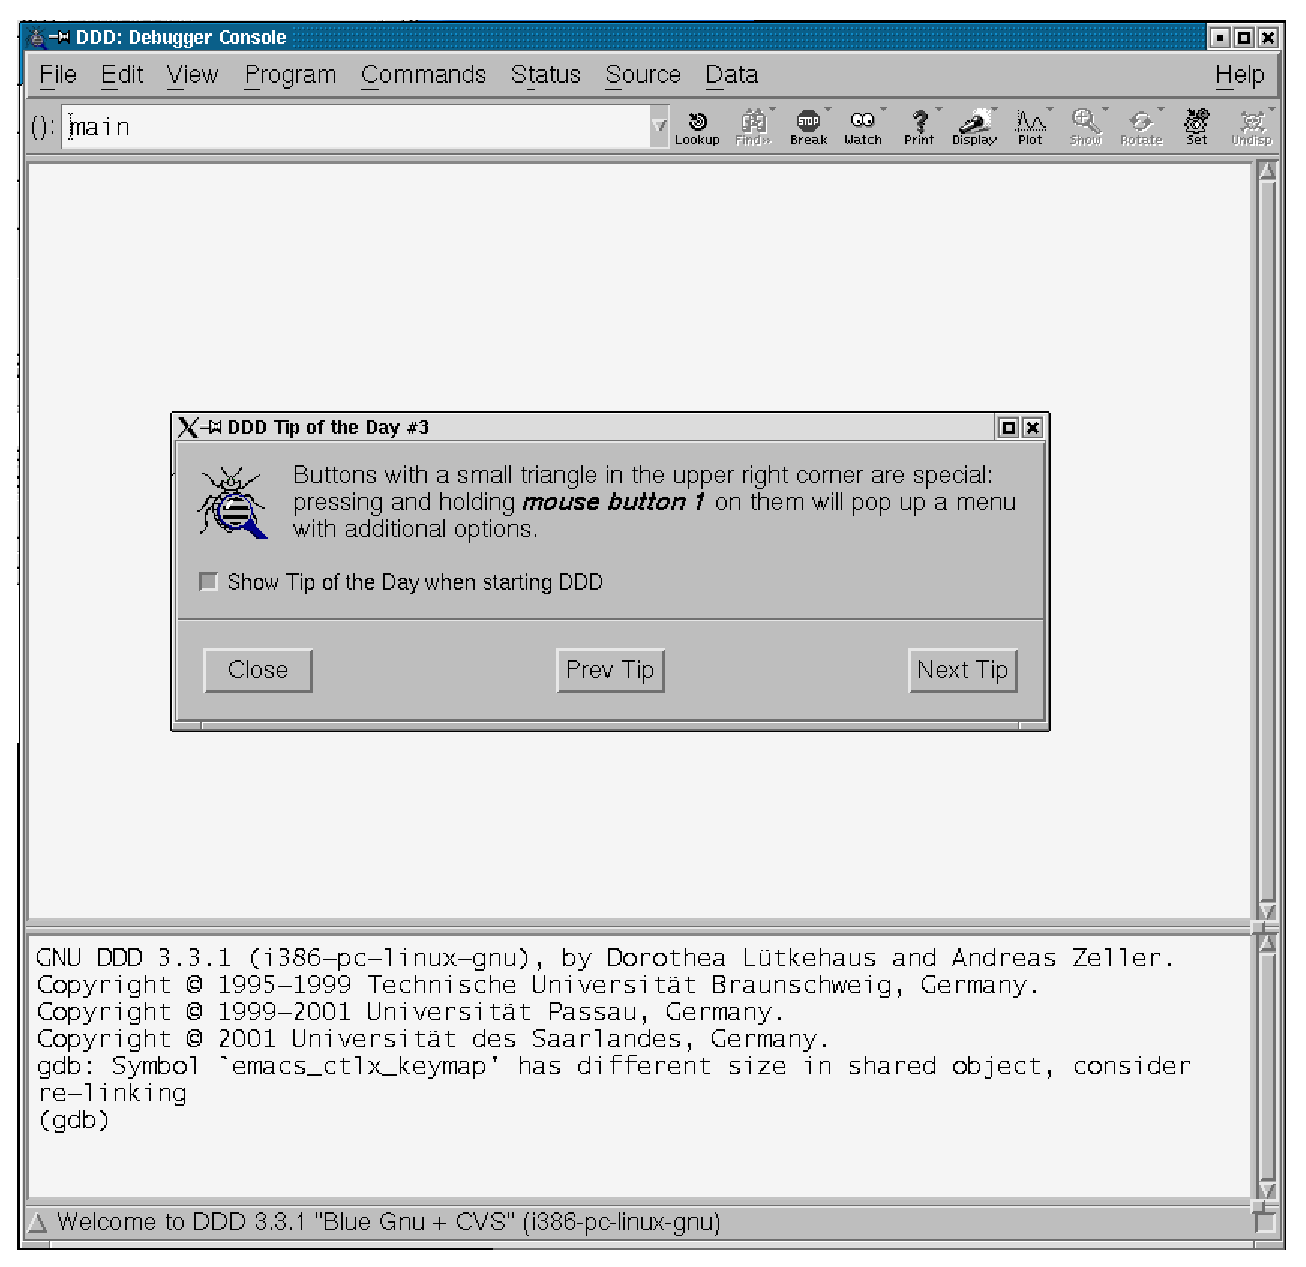
\includegraphics[width=\textwidth]{imagenes/ddd_inicio.eps}
\caption{Pantalla de inicio}
\end{figure}

Este es  el aspecto que  presenta el  {\tt ddd} cuando  lo arrancamos,
vamos a ir por pasos mostrando  lo que normalmente un programador como
nosotros vamos a necesitar de un depurador.

\subsection{Mostrar el contenido de las variables}

Para mostrar el contenido de las  variables lo que tendremos que hacer
es, como se dice coloquialmente, colocar un {\em watch} a la variable.
En {\tt ddd} esto  es muy sencillo de hacer y  hay varias maneras, una
de ellas puede ser  escribir el nombre de la variable  en el cuadro de
texto que  tenemos justo por  debajo de la barra  de men� y  pulsar el
bot�n de watch que est� al mismo nivel un poco m�s a la derecha:

\begin{figure}[hbtp]
\centering
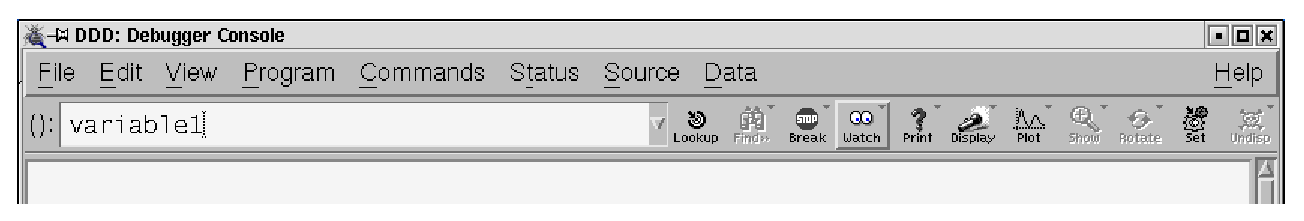
\includegraphics[width=\textwidth]{imagenes/ddd_watch.eps}
\caption{Barra de herramientas}
\end{figure}

Otra forma de hacerlo quiz� m�s r�pida poner el cursor del rat�n sobre
el nombre de la variable en  el c�digo fuente, pulsar el boton derecho
y escoger la opcion display.

\begin{figure}[hbtp]
\centering
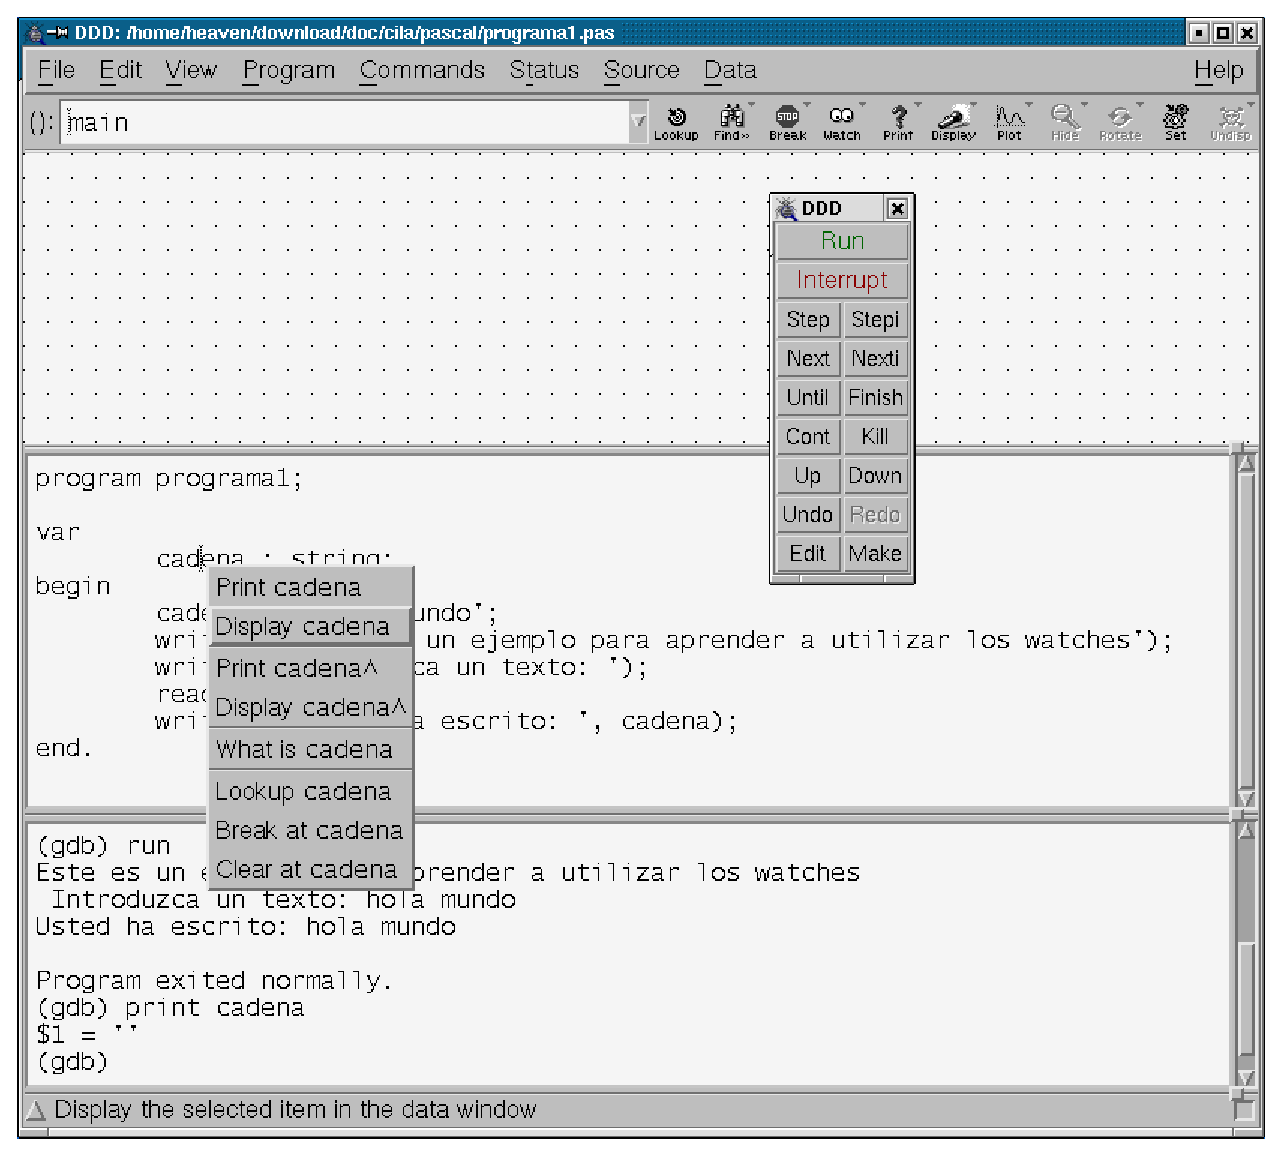
\includegraphics[width=\textwidth]{imagenes/ddd_watchII.eps}
\caption{Watches}
\end{figure}

\subsection{Colocar puntos de  ruptura (Breakpoints)}
\index{Depuradores!puntos de ruptura}

Bueno, ya tenemos un watch de la variable, pero\ldots �que pasa cuando
pulsamos sobre el bot�n de run? �No vemos nada! Bueno, eso es una
circunstancia pasajera, vamos a colocar un {\em punto de ruptura} o
punto de ruptura.

Los puntos de ruptura son lugares donde el depurador har� que nuestro
programa pare la ejecucu�n para, de esta manera, analizar detenidamente
el estado de nuestro programa. La manera de colocar un punto de ruptura
en el {\tt ddd} es simplemente desplazarse hasta la l�nea donde deseamos
colocar el punto de ruptura y hacer un doble click con el boton
izquierdo del rat�n.

Vemos que se nos coloca un s�mbolo de stop donde hemos hecho el doble
click, lo que indica que hay un punto de ruptura. Si pulsamos sobre el
punto de ruptura con el boton derecho vemos que se nos da la opcion
de desactivarlo, quitarlo y una muy extra�a de propiedades. La opcion
de propiedades hace que nos aparezca un cuadro de dialogo en el cual
podemos introducir una expresi�n, �sta expresi�n se utiliza para hacer
que nuestro punto de ruptura sea inteligente y no pare la ejecuci�n
siempre que el programa pase por all�, sino que solo se parar� cuando
la expresi�n se cumpla, por ejemplo, si ponemos el punto de ruptura en
un bucle con 10.000 iteraciones y nosotros queremos que se pare cuando
la i (variable que cuenta las iteraciones) llegue a 5000 pues lo que
hemos de poner en propiedades del punto de ruptura es {\tt i = 5000} y
de esa manera nos saltaremos las 5000 primeras iteraciones que no nos
interesan.

\begin{figure}[hbtp]
\centering
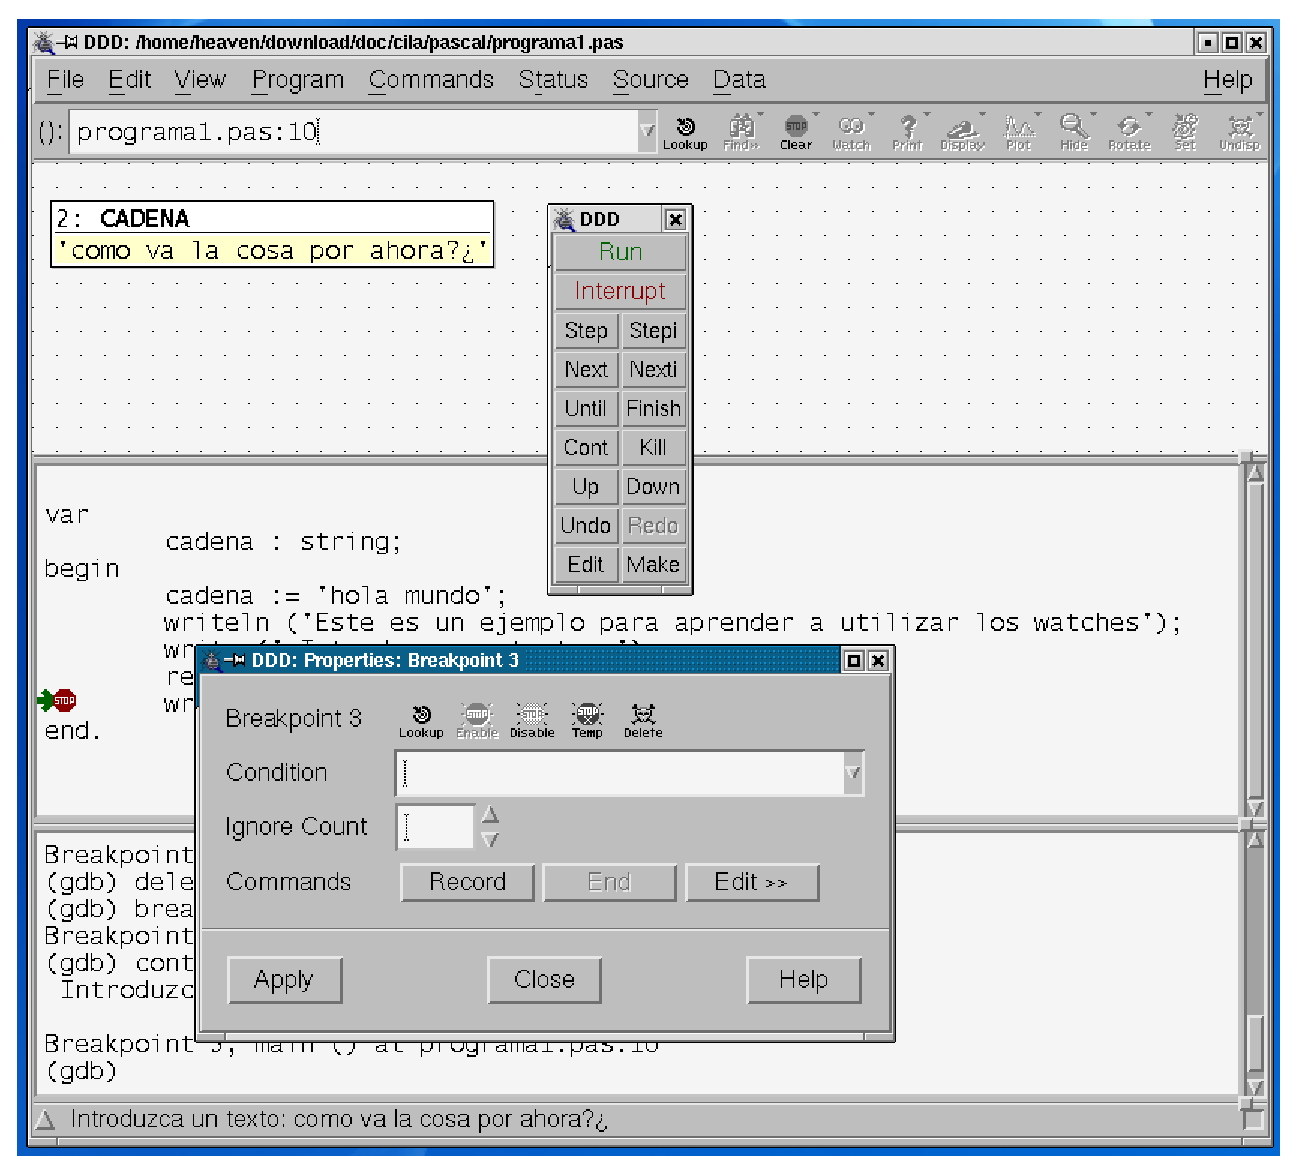
\includegraphics[width=\textwidth]{imagenes/ddd_breakpoint.eps}
\caption{Breakpoints, o puntos de ruptura}
\end{figure}

\subsection{Ejecuci�n paso a paso}
\index{Depuradores!ejecuci�n paso a paso}

Ahora que ya tienes un watch y un punto de ruptura, en este momento
solo podemos ir saltanto de punto de ruptura en punto de ruptura, y
esto no nos es suficiente as� que vamos a intentar controlar m�s el
flujo de ejecuci�n de nuestros programas. Para esta tarea tenemos varias
herramientas comunes en la mayor�a de depuradores, en el caso del dd las
encontramos en una ventana que tenemos flotando sobre el depurador, con
lo cual no es complicado utilizarlas, siempre las tenemos a mano y son
las siguientes:

\begin{description}

\item[{\em Step}:]{(paso) esta herramienta nos sirve, como su propio
nombre indica, para ejecutar nuestro programa paso a paso. Normalmente
lo que hacemos es colocar un punto de ruptura al inicio de la funcion o
procedimiento que queremos analizar y luego ir pulsando {\tt step} para
analizar sentencia a sentencia que es lo que hace nuesto c�digo.}

\item[{\em Next}:]{(siguiente) muy parecida a step, solo que pulsando
{\tt next} si en el c�digo hay una llamada a una funcion o procedimiento
no entramos en ella, sino que ejecuta �sta y nos colocamos en la
siguiente l�nea del programa.}

\item[{\em Until}:]{(hasta) esta herramienta nos sirve para ejecutar el
programa hasta la posici�n actual del cursor, es muy parecida a un punto
de ruptura temporal.}

\item[{\em Cont}:]{(continuar) saltamos hasta el siguiente punto de
ruptura o hasta el final del programa si es que no hay ning�n punto de
ruptura m�s en el flujo de ejecuci�n.}

\end{description}

A  parte de  estas  herramientas  tenemos algunas  m�s  que se  suelen
utilizar  menos, por  ejemplo  aquellas que  ejecutan exactamente  una
instrucci�n (de c�digo m�quina).

\subsection{Visi�n de punteros}
\index{Depuradores!visi�n de punteros}

Probablemente estabas deseando que existiera  una cosa como la que vas
a ver. No te asombres de la  potencia de este depurador, es uno de los
pocos que lo  hacen y de ah�  viene su buena fama. La  capacidad de la
que hablamos es la de {\em ver} los punteros.

Seguramente has hecho  m�s de un programa con memoria  din�mica que no
acababa de  funcionar bien porque se  te perd�an punteros y  no sabias
muy bien  por donde andaban  o a  d�nde estaban apuntando,  pues bien,
esto ya no es excusa para entregar una pr�ctica a medio hacer, el {\tt
ddd} viene en nuestra ayuda  y tenemos la {\em herramienta definitiva}
para la depuraci�n con punteros.\\

Cuando  haces un  watch de  una  estructura (record)  salen todos  los
campos en un  recuadro y los punteros tambi�n salen  como otro tipo de
dato  cualquiera. Cuando  tienes {\tt  \$0}  en la  informaci�n de  un
puntero quiere  decir que  el puntero  es {\tt  Nil} (nulo),  y cuando
tenemos un n�mero  precedido del s�mbolo {\tt \$} quiere  decir que el
puntero est� apuntando  a esa zona de memoria, por  lo tanto, podremos
mostrar el  contenido de esa  zona de memoria. Si  decidimos mostrarla
aparecer�  otro cuadro,  como  el que  inicialmente  ten�amos, con  la
informaci�n de  la zona de memoria  apuntada por el puntero  que hemos
decidido expandir  y una  flecha desde el  recuadro original  hasta el
nuevo, marcada con el nombre del puntero expandido.

De  esta manera  es  muy sencillo  seguir  los punteros  y  ver a  que
posiciones est�n apuntando, ver si  estamos asignando cosas a punteros
que son nulos as� como que pinta va teniendo la estructura que estamos
construyendo en memoria, lo cual ayuda  mucho a la hora de moverse por
las estructuras que fabricamos.

Un ejemplo  de lo  que se puede  hacer es mostrar  un �rbol  para, por
ejemplo, comprobar que todos los  punteros que salen de nuestros nodos
hoja est�n  a {\tt  Nil} y  de esa manera  asegurarnos de  que nuestro
programa no va a fracasar.

\begin{figure}[hbtp]
\centering
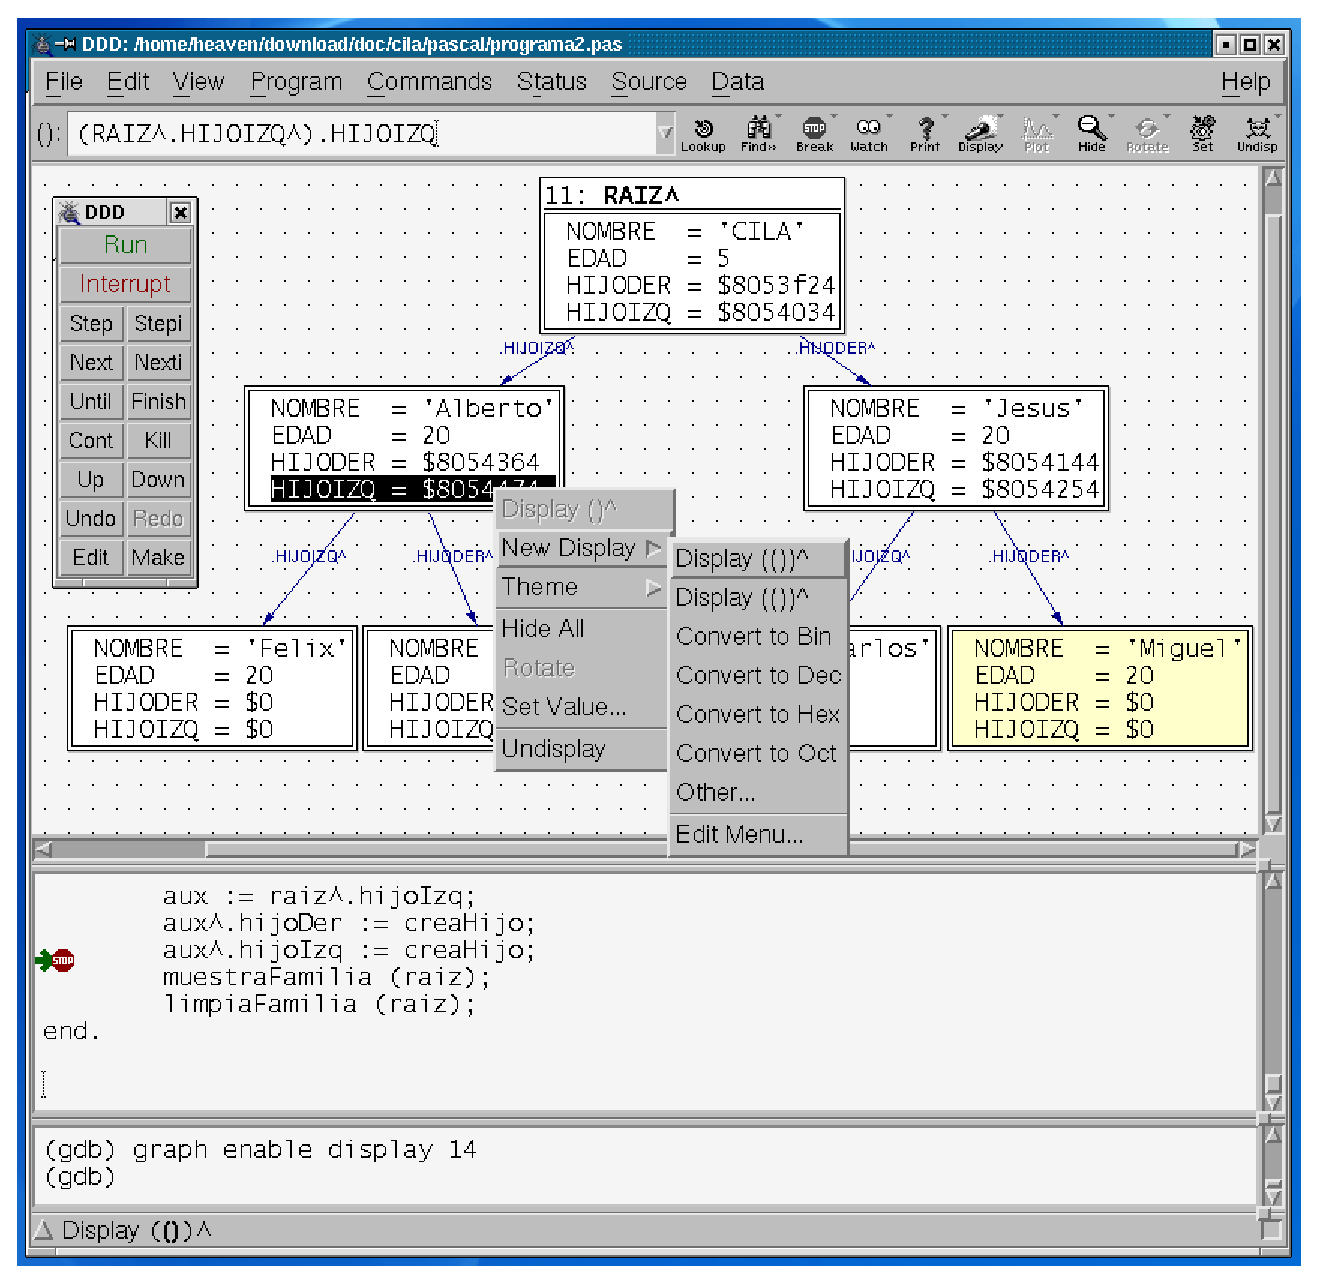
\includegraphics[width=\textwidth]{imagenes/ddd_punteros.eps}
\caption{Estructura de un �rbol binario}
\end{figure}


% M�dulo VI:  Programaci�n avanzada
% 1. PHP + [My|Postgre]SQL
% 2. Perl
% 3. Python (NumPy) 
% 4. GUIs toolkits: Tk, QT, Wx, Gtk, Glade
% 5. XML
\part{Programaci�n avanzada}
%Autor: Carlos de la Cruz (frodo@fmat.ull.es)

\chapter{PHP}

\section{Introducci�n}
PHP es un lenguaje dise�ado para la generaci�n din�mica de p�ginas web.
Los ficheros de PHP se almacenan en el servidor y se ejecutan cuando un usuario introduce en su navegador la direccion de una de estas p�ginas. Estas, a su vez, contienen c�digo a partir del cual se generan p�ginas est�ticas en formato HTML.

La utilidad de esto es que podemos crear autom�ticamente p�ginas web que se actualicen solas, bas�ndose en una fuente de datos.

Por ejemplo, si quisi�ramos que cada vez que el usuario accede a nuestra p�gina, en esta apareciera la fecha y la hora, ser�a imposible conseguirlo a partir de ficheros est�ticos ``html''.

Por tanto, la soluci�n ser�a tener en el servidor un fichero ``hora.php'', mediante el cual, cuando alguien accediera a: http://miservidor.com/hora.php, tuviera la hora del instante en que se ejecut� el c�digo php.

Cada vez que alguien le diera a ``recargar'' en el navegador, ver�a la hora actual.

Pero como podremos comprobar,si se hace clic en el bot�n ``ver c�digo fuente'' del navegador, s�lo veremos, por ejemplo ``12:02:12''.

PHP tiene todas las ventajas que tienen otros lenguajes utilizados para generaci�n din�mica de contenido web como PERL y ASP, y otras que ninguno de estos permiten hacer de una forma flexible y c�moda, como por ejemplo la generaci�n din�mica de pel�culas Macromedia Flash, im�genes (con el m�dulo GDLib), informes en formato PDF, etc.

\section{Primeros Pasos}

Todo script php est� delimitado por los identificadores {\tt<?php y ?>}. Dentro de estos s�mbolos, va escrito todo el c�digo php de este.

La primera funci�n que veremos de PHP ser� ''echo'', que nos permite imprimir
texto o tags HTML en nuestra p�gina. La funci�n echo va siempre acompa�ada de
unos par�ntesis y comillas(simples o dobles) en caso de que vayamos a imprimir una o varias cadenas est�ticas de texto, y puede ir o no acompa�ada de estos en caso de que vayamos a imprimir s�lo el contenido de una o varias variables.


Como con el resto de los lenguajes, vamos a empezar viendo como ser�a un "hola mundo" en PHP.

\begin{verbatim}
<?php

echo("<center><font size=7>Hola, Mundo!</font></center>");

?>
\end{verbatim}

Este sencillo script nos permite ver como diferenciar el c�digo PHP del c�digo HTML, pues si introduj�ramos c�digo HTML suelto dentro de los delimitadores {\tt <?php y ?>}, el m�dulo PHP de nuestro servidor web provocar�a un error de interpretaci�n.

PHP es un lenguaje muy flexible. Nos permite imprimir el valor de variables
dentro de cadenas de texto sin tener que cerrar y volver a abrir comillas, de
la siguiente forma:
\begin{verbatim}
<?php

$limones=2;
$naranjas=3;

echo("Tenemos $limones limones y $naranjas naranjas.");
?>

\end{verbatim}

F�jate que no es lo mismo escribir:
{\tt echo("Tenemos $limones limones y $naranjas naranjas."); } que
{\tt echo('Tenemos $limones limones y $naranjas naranjas."); }.

La primera l�nea, para $limones=2 y $naranjas=3 imprimir� "Tenemos 2 limones y 3 naranjas", mientras que la segunda imprimir� ''Tenemos $limones limones y $naranjas naranjas". Es decir, si utilizamos las dobles comillas, tendremos que los valores de las variable se despliegan dentro de estas. Si utilizamos, por el contrario, comillas simples, lo que haya entre ellas se imprimir� tal cual.

Es importante saber que cuando uno necesita utilizar comillas en el HTML resultante de nuestro script PHP, conviene que ''escape'' las comillas, o de lo contrario el interpretador mostrar� una p�gina con un error de compilaci�n.

por ejemplo, si queremos mostrar el tag html:

{\tt <a href="http://www.fmat.ull.es/~frodo">}, tendremos que hacerlo de la siguiente forma en php:
{\tt echo("<a href=\"http://www.fmat.ull.es/~frodo\">");}. (F�jate en las barras invertidas que se anteponen a cada una de las comillas que van dentro del par de comillas de la funci�n "echo".

Para la inclusi�n de c�digo HTML previamente escrito dentro de una p�gina que se genera din�micamente (por ejemplo, sup�n que tienes una cabecera, un pie de p�gina predefinidos para tu sitio web, y quieres que var�e s�lo el cuerpo de la p�gina, para darle un dise�o uniforme), utilizamos el comando {\tt include}.

Por ejemplo:

\begin{verbatim}
<?php

include "include/cabecera.php";
echo("Hola! este es el cuerpo de la p�gina");
include"include/pie.php;

?>

\end{verbatim}





\section{Estructuras de datos}

B�sicamente, existen los escalares, los hash y los arrays.


\section{Estructuras de control}

Para el uso de las estructuras de control PHP es muy parecido al lenguaje ''C'', tanto por el uso de llaves para delimitar los bloques de c�digo como por usar la misma sintaxis. Distinguiremos dos tipos de estructuras de control:

\subsection{Condicionales: If, Switch}

If: Este condicional nos permite ejecutar un bloque de c�digo en caso de que se
de una condici�n determinada. Veamos un ejemplo:

\begin{verbatim}
<?php

$a = 2;
$b = 10;

if ($a<$b) {
	echo("Hey!, parece que \$a vale $a, que es mayor que \$b, que vale $b");
	}
	
?>

Como, evidentemente 2 siempre ser� menor que 10, el bloque de c�digo entre llaves se ejecutar�a siempre.

\end{verbatim}

\subsection{Repetitivas: While,For}

\section{Como estructurar nuestro c�digo en php}

Las funciones. function chona($lalala,$otroparametro)

\section{Manejo de formularios}


\section{Utilizaci�n de bases de datos}
Aunque PHP soporta varias clases de servidores de base de datos, debido a que cada uno usa un interfaz distinto, resulta bastante inc�modo tener que aprender las funciones de PHP para cada uno de ellos. Es por ello que suelen utilizarse librer�as adicionales (no incluidas con PHP, pero s� con la mayor�a de las distribuciones Linux), como la que utilizaremos en este texto/curso: AdoDB.

AdoDB nos permite cambiar de sistema de bases de datos simplemente cambiando un par�metro al realizar la conexi�n a la Base de datos (BDD de ahora en adelante) , de forma que una aplicaci�n PHP dise�ada para correr con Oracle, puede ser portada para funcionar en MySql, Informix, etc. con tan s�lo cambiar una l�nea de c�digo.


\section{Creaci�n de im�genes din�micamente}

\section {Bibliograf�a recomendada}



%Autor: MojoPiKon

\chapter{Perl}

\section{Que es PERL}

PERL es un lenguaje de scripts o guiones creado por Larry Wall en 1988, que, a pesar de haber tenido su m�xima difusi�n con la aparici�n de internet y el web, viene siendo utilizado desde hace varios a�os por administradores de sistemas para la automatizaci�n de tareas rutinarias, como pueden ser gesti�n de grandes vol�menes de usuarios, b�squeda de patrones de texto mediante expresiones regulares, realizaci�n de copias selectivas de seguridad, etc.

% Existen una enorme variedad de m�dulos para PERL (baste decir el listado de ellos en texto plano ocupa varios megabytes). Tanto este listado como estos m�dulos pueden encontrarse en la web de recursos para perl http://www.cpan.org

Como lenguaje interpretado, su potencia radica en su gran portabilidad siempre que los m�dulos que se empleen se encuentren en la plataforma en que el script vaya a ser utilizado.

Pese a la creencia popular, PERL sirve para desarrollar casi cualquier tipo de programa, pues entre sus m�dulos se encuentran, por poner algunos ejemplos, m�dulos de OpenGL (Especificaci�n para la creaci�n de gr�ficos 3D),para el tratamiento de audio digital, o para la creaci�n de interfaces gr�ficas, ya sea bajo plataformas corriendo sistemas GNU/Linux,Variantes de UNIX,Apple MacOs, Microsoft Windows, etc.

\section{Donde conseguir PERL}

La versi�n oficial de PERL est� disponible de forma gratuita en la web oficial del proyecto PERL (http://www.perl.org) para las distintas plataformas anteriormente citadas.

Por otro lado, hay distribuciones empaquetadas por empresas, con algunos m�dulos m�s que la versi�n oficial ``base''.

Destaca por su comodidad de instalaci�n y la cantidad de m�dulos disponibles ``activeperl'', de activestate (http://www.activestate.com).

Activeperl est� disponible para Linux y para Windows, y puede ser descargado tambi�n de forma gratuita.

\section{Primeros pasos}

PERL lee los scripts a partir de ficheros de texto plano. Para ejecutarlos, suele procederse de la siguiente manera:

\begin{verbatim}

14:16:14 wd:~ u:frodo> perl fichero.pl

\end{verbatim}

Esto ejecuta el gui�n contenido en el fichero ``fichero.pl''. Esto no resulta muy sorprendente, desde luego.

Para ejecutar scripts PERL en GNU/Linux o UNIX, podemos recurrir a colocar al principio del gui�n una l�nea como esta:

\begin{verbatim}

#!/usr/bin/perl

\end{verbatim}

Con esto conseguiremos, tras dar permisos de ejecuci�n al script mediante chmod 755 fichero.pl, poder ejecutarlo poniendo desde el shell:

\begin {verbatim}

./programa.pl

\end{verbatim}

Para probar que realmente nuestro int�rprete PERL funciona correctamente, probemos un apasionante y a la vez complejo programa:

\begin {verbatim}

#!/usr/bin/perl / 
print ``Hola mundo!\n'';

\end{verbatim}

\section{Entrada,salida y sint�xis b�sica}

La sint�xis de PERL a muchos programadores nos recuerda a la de C, por que emplea llaves ``{ }'', puntos y comas al final de las l�neas, e incluso gran parte
de las estructuras de control de C, las cuales se manejan de forma casi id�ntica en ambos lenguajes, y que veremos en el siguiente apartado. 

Para insertar comentarios en nuestro c�digo, emplearemos el caracter de ``almohadilla''.

\begin{verbatim}
# Esto es un comentario en PERL. Esta l�nea no hace nada, pero tampoco
# provoca errores de compilaci�n en nuestro programa.
\end{verbatim}

Las variables en PERL son de tres tipos: arrays, escalares y estructuras ``hash''. Estas ser�n descritas en profundidad en la secci�n ``Estructuras de datos, de control y operadores''. De momento, nos contentaremos con saber que los escalares son variables que s�lo almacenan UN dato y que pueden contener datos num�ricos, cadenas ascii, etc y que se denotan anteponiendo a su nombre un signo de dolar. Se aplican las normas estandar de otros lenguajes para nombrar estas variables, como son no utilizar n�meros al principio del identificador, no utilizar espacios y no utilizar palabras reservadas como identificadores.
Cualquier omisi�n en el cumplimiento de estas normas provocar� irremisiblemente un error de interpretaci�n.


Se puede hacer corresponder a una variable de tipo escalar una cadena mediante el uso de el igual y las comillas simples. Para los valores num�ricos se pone s�mplemente el igual y el valor, sin comillas. Ejemplo:

\begin{verbatim}

$nombre = 'Fernando';
$edad = 19;
$numero_de_piso = '5';


\end{verbatim}

N�tese que si pusieramos las comillas para asignar un valor num�rico a una variable escalar, PERL interpretar�a dicha variable como una cadena de caracteres ASCII, por lo que no podr�amos, por ejemplo, sumar o restar dichos n�meros.

Es importante conocer que podemos utilizar tanto comillas simples como comillas dobles para asignar cadenas a escalares. Pero existe una diferencia.

\begin{verbatim}
$nombre = ``Carlos'';

print''Me llamo $nombre\n''; # Imprime: Me llamo Carlos
print 'Me llamo $nombre''; # Imprime: Me llamo $nombre\n

\end{verbatim}


Ahora que ya sabemos lo b�sico de las reglas del juego, veamos algo m�s sobre la funci�n print.





\section{Estructuras de control, de datos y operadores}





\section{Manejo de Cadenas}

\section{Ficheros}

\section{Automatizaci�n de tareas y ejecuci�n de comandos externos}

\section{Interfaces b�sicas de usuario en modo texto}

\section{Bibliograf�a recomendada}


%Autor: miguev

\chapter{Python}



\chapter{GUIs y toolkits}


\chapter{XML}



% Ap�ndices y referencias
\appendix
%Autor: todos
  
\chapter{Recursos en internet}
  

La mayor�a  de los recursos que  podamos necesitar para usar  Linux se
encuentran  distribuidos por  Internet,  y una  enorme cantidad  est�n
disponibles en espa�ol.

\begin{itemize}

\item {\tt http://www.debian.org} -- El Proyecto Debian es una asociaci�n
  de  personas  que  han  hecho  causa com�n  para  crear  un  sistema
  operativo (SO)  libre. Este  sistema operativo  que hemos  creado se
  llama Debian GNU/Linux, o simplemente Debian para acortar.

\item {\tt http://www.redhat.es} --  La  primera  distribuci�n Linux  en
  reorientarse hacia los usuarios finales.

\item {\tt http://www.linux-mandrake.com/es/} -- Linux-Mandrake es
  un amigable Sistema Ope\-ra\-ti\-vo Linux. Es  muy f�cil de usar, tanto en
  el  hogar u oficina  como en servidores. Est�  disponible  en  forma
  gratuita en varios idiomas alrededor del mundo.

\item {\tt http://www.ututo.org} -- Un GNU/Linux Simple.

\item {\tt http://www.linux-es.com} -- Existen muchos lugares en
  Internet  dedicados  a  LINUX,  pero  la mayor�a de ellos est�n en
  ingl�s. Estas p�ginas  pretenden  ser un  punto  de  partida  para
  aquellos  que necesitan encontrar informaci�n sobre este sistema y
  en  la  medida de lo posible se ha intentado que la mayor�a de los
  enlaces y contenidos sean en castellano.

\item {\tt http://www.gnu.org/home.es.html} -- El  Projecto  GNU
  comenz� en  1984 para  desarrollar un sistema  operativo tipo Unix
  completo, el cual  es  software libre:  El  sistema  GNU. Variantes
  del  sistema GNU, utilizando Linux  como  kernel,  son  ampliamente
  usadas, y aunque frecuentemente llamadas ``Linux'', dichas variantes
  deber�an referirse m�s exactamente como sistemas GNU/Linux.

\item {\tt http://lucas.hispalinux.es}  --  Proyecto LuCAS  -  La
  mayor biblioteca en espa�ol dedicada a GNU/LiNUX de todo el planeta

\item {\tt http://www.insflug.org}  --  En  el INSFLUG  se  coordina
  la traducci�n ``oficial'' de documentos  breves, como los COMOs  y
  PUFs o  Preguntas de Uso Frecuente, las FAQs  en ingl�s. Esperamos
  que la informaci�n que encuentre aqu� le sea de utilidad.

\item {\tt http://www.gnu.org/software/emacs/emacs.html} --  Es un
  editor de  pantalla y  ambiente  para c�mputo  de  tiempo real,
  extensible  y  personalizable.  Ofrece Lisp (finalmente integrado al
  editor)  para escribir  extensiones  y proporciona  una interfaz  al
  sistema de ventanas X.

\item {\tt http://www.vim.org} -- VIM es  una versi�n mejorada del
  editor VI, uno de los editores de texto est�ndar en los sistemas UNIX.
  VIM a�ade muchas de las  caracter�sticas que se  esperan en  un editor:
  Deshacer ilimitado, coloreado de sintaxis, GUI, y mucho m�s.

\item \label{putty}{\tt http://www.chiark.greenend.org.uk/~sgtatham/putty/} --
  Implementaci�n libre de un cliente TELNET/SSH para sistemas operativos
  Microsoft� Windows�. Escrito y mantenido por Simon Tatham.

\item {\tt http://www.escomposlinux.org/sromero/linux/} -- S.O.S. Linux.

\item  {\tt http://www.geocities.com/Athens/Temple/2269/}  -- Tutorial
de C/C++

\item {\tt http://www.fie.us.es/docencia/publi/JAVA/} -- Tutorial de Java

\item {\tt http://apolo.us.es/CervanTeX/} -- Informaci�n LaTeX en espa�ol

\item {\tt ftp://ftp.cma.ulpgc.es/pub/software/TeX/tex/latex2e/doc/ldesc2e/mix/ldesc2e.pdf} -- Una descripci�n de LaTeX, por Tom�s Bautista y cia.

\item {\tt http://www.lyx.org}  --  P�gina del proyecto LyX 

\item {\tt http://www.octave.org}  --  P�gina del proyecto Octave

\item {\tt http://www.gnuplot.org}  --  P�gina del proyecto Gnuplot

\item {\tt http://www.r-project.org} -- P�gina del proyecto R

\item {\tt http://yacas.sourceforge.net} -- P�gina del proyecto Yacas

\item {\tt http://www-rocq.inria.fr/scilab/}  --  P�gina del proyecto SciLab

\item {\tt http://www.lysator.liu.se/\~alla/dia/} --  P�gina del proyecto DIA

\item {\tt http://www.gimp.org} --  P�gina del proyecto GIMP

\item {\tt http://www.qcad.org} -- P�gina del proyecto QCad

\item {\tt http://www.linuxfocus.org/Castellano/January2002/article132.shtml} -- Tutorial 
de {\sf QCad} en Castellano.

\end{itemize}




\chapter{Licencia de Documentaci�n Libre GNU}

\label{GFDL}

Versi�n 1.1, Marzo de 2000

�sta es la GNU Free Document  License (GFDL), versi�n 1.1 (de marzo de
2000),  que cubre  manuales  y  documentaci�n para  el software  de la
Free  Software  Foundation,  con  posibilidades en  otros  campos.  La
traducci�n  \footnote{N.  del T.  Derechos  Reservados  en el  sentido
de   GNU  \htmlurl{http://www.gnu.org/copyleft/copyleft.es.html}}   no
tiene  ning�n  valor  legal,  ni  ha  sido  comprobada  de  acuerdo  a
la  legislaci�n de  ning�n  pa�s  en particular.  Vea  el original  en
\htmlurl{http://www.gnu.org/copyleft/fdl.html}

Los autores de esta traducci�n son:

\begin{itemize}
\item Igor T�mara (\htmlurl{ikks@bigfoot.com})
\item Pablo Reyes (\htmlurl{reyes\_pablo@hotmail.com})
\item Revisi�n: Vladimir T�mara P. (\htmlurl{vtamara@gnu.org})
\end{itemize}

\begin{quote}
Copyright $\copyright$ 2000  Free Software Foundation, Inc.\\
      59 Temple Place, Suite 330, Boston, MA  02111-1307  USA\\
  Everyone is permitted to copy and distribute verbatim copies
  of this license document, but changing it is not allowed.
\end{quote}
  Se permite la copia y distribuci�n de copias literales
  de este documento de licencia, pero no se permiten cambios.
  
 
\section*{Pre�mbulo}

El prop�sito  de esta  licencia es  permitir que  un manual,  libro de
texto,  u  otro documento  escrito  sea  ``libre''  en el  sentido  de
libertad: asegurar a todo el mundo  la libertad efectiva de copiarlo y
redistribuirlo, con o sin modificaciones, de manera comercial o no. En
segundo t�rmino,  esta licencia  preserva para el  autor o  para quien
publica una manera de obtener reconocimiento por su trabajo, al tiempo
que no se consideran responsables de las modificaciones realizadas por
terceros.

Esta licencia  es una  especie de ``copyleft''  que significa  que los
trabajos derivados del documento deben a su vez ser libres en el mismo
sentido. Esto complementa la Licencia  P�blica General GNU, que es una
licencia de copyleft dise�ada para el software libre.


Hemos  dise�ado esta  Licencia  para usarla  en  manuales de  software
libre,  ya que  el  software libre  necesita  documentaci�n libre:  Un
programa  libre debe  venir con  los manuales  que ofrezcan  la mismas
libertades  que da  el software.  Pero esta  licencia no  se limita  a
manuales de software; puede ser  usada para cualquier trabajo textual,
sin tener  en cuenta su tem�tica  o si se publica  como libro impreso.
Recomendamos esta  licencia principalmente para trabajos  cuyo fin sea
instructivo o de referencia.


\section{Aplicabilidad y definiciones}

Esta  Licencia se  aplica  a  cualquier manual  u  otro documento  que
contenga  una  nota  del  pro\-pie\-ta\-rio  de  los  derechos  que  indique
que  puede  ser distribuido  bajo  los  t�rminos  de la  Licencia.  El
``Documento'', en adelante, se refiere a cualquiera de dichos manuales
o trabajos. Cualquier miembro del  p�blico es un licenciatario, y ser�
denominado como ``Usted''.

Una ``Versi�n  Modificada'' del Documento significa  cualquier trabajo
que contenga  el Documento o una  porci�n del mismo, ya  sea una copia
literal o con modificaciones y/o traducciones a otro idioma.

Una  ``Secci�n Secundaria''  es  un ap�ndice  titulado  o una  secci�n
preliminar al pr�logo  del Documento que tiene  que ver exclusivamente
con la  relaci�n de quien publica,  o los autores del  Documento, o el
tema general del Documento(o asuntos relacionados) y cuyo contenido no
entra directamente en este tema general. (Por ejemplo, si el Documento
es en parte  un texto de matem�ticas, una Secci�n  Secundaria puede no
explicar matem�ticas.)  La relaci�n  puede ser  un asunto  de conexi�n
hist�rica,  o  de  posici�n  legal,  comercial,  filos�fica,  �tica  o
pol�tica con el tema o la materia del texto.

Las ``Secciones Invariantes'' son  ciertas Secciones Secundarias cuyos
t�tulos son  denominados como  Secciones Invariantes,  en la  nota que
indica que el documento es liberado bajo esta licencia.

Los ``Textos de Cubierta'' son ciertos  pasajes cortos de texto que se
listan, como Textos de Portada o  Textos de Contra Portada, en la nota
que indica que el documento est� liberado bajo esta Licencia.

Una  copia ``Transparente''  del Documento,  significa una  copia para
lectura  en m�quina,  representada en  un formato  cuya especificaci�n
est� disponible al p�blico general, cuyos contenidos pueden ser vistos
y  editados  directamente con  editores  de  texto gen�ricos  o  (para
im�genes compuestas por  pixeles) de programas gen�ricos  de dibujo o
(para dibujos) alg�n editor gr�fico  ampliamente disponible, y que sea
adecuado  para exportar  a formateadores  de texto  o para  traducci�n
autom�tica  a  una variedad  de  formatos  adecuados para  ingresar  a
formateadores de  texto. Una copia hecha  en un formato de  un archivo
que no sea Transparente, cuyo formato  ha sido dise�ado para impedir o
dificultar subsecuentes  modificaciones posteriores  por parte  de los
lectores no es  Transparente. Una copia que no  es ``Transparente'' es
llamada ``Opaca''.

Como ejemplos de formatos adecuados para copias Transparentes est�n el
ASCII plano sin formato, formato de  Texinfo, formato de LaTeX, SGML o
XML usando un DTD disponible ampliamente,  y HTML simple que sigue los
est�ndares, dise�ado para modificaciones  humanas. Los formatos Opacos
incluyen PostScript, PDF, formatos  propietarios que pueden ser le�dos
y editados unicamente en procesadores de palabras propietarios, SGML o
XML para los cu�les los DTD y/o herramientas de procesamiento no est�n
disponibles generalmente, y el HTML  generado por m�quinas producto de
alg�n procesador de palabras solo para prop�sitos de salida.

La ``Portada'' en un libro  impreso significa, la propia portada junto
con las p�ginas siguientes necesarias para mantener la legibilidad del
material, que esta Licencia requiere  que aparezca en la portada. Para
trabajos  en formatos  que  no tienen  Portada  como tal,  ``Portada''
significa el texto junto a la  aparici�n m�s prominente del t�tulo del
trabajo, precediendo el comienzo del cuerpo del trabajo.


\section{Copia literal}

Puede  copiar y  distribuir el  Documento en  cualquier medio,  sea en
forma comercial  o no, siempre  y cuando  esta Licencia, las  notas de
derecho de autor,  y la nota de licencia que  indica que esta Licencia
se aplica al Documento se reproduzca  en todas las copias, y que usted
no  adicione  ninguna  otra  condici�n  a las  expuestas  en  en  esta
Licencia. No puede usar medidas  t�cnicas para obstruir o controlar la
lectura o copia  posterior de las copias que usted  haga o distribuya.
Sin embargo, usted puede aceptar  compensaci�n a cambio de las copias.
Si  distribuye  un n�mero  suficientemente  grande  de copias  tambi�n
deber� seguir las condiciones de la secci�n 3.

Tambi�n puede prestar copias, bajo las mismas condiciones establecidas
anteriormente, y puede exhibir copias publicamente.

\section{Copiado en cantidades}

Si publica copias impresas del Documento  que sobrepasen las 100, y la
nota de Licencia del Documento  exige Textos de Cubierta, debe incluir
las copias  con cubiertas que lleven  en forma clara y  legible, todos
esos textos  de Cubierta: Textos  Frontales en la cubierta  frontal, y
Textos  Posteriores  de  Cubierta  en  la  Cubierta  Posterior.  Ambas
cubiertas deben identificarlo a Usted  clara y legiblemente como quien
publica  tales copias.  La  Cubierta Frontal  debe  mostrar el  t�tulo
completo  con todas  las palabras  igualmente prominentes  y visibles.
Adem�s puede  a�adir  otro  material  en  la cubierta. Las  copias con
cambios limitados  en las cubiertas,  siempre que preserven  el t�tulo
del Documento y satisfagan  estas condiciones, puede considerarse como
copia literal.

Si los textos requeridos para la cubierta son muy voluminosos para que
ajusten  legiblemente,  debe colocar  los  primeros  (tantos como  sea
razonable  colocar) en  la  cubierta  real, y  continuar  el resto  en
p�ginas adyacentes.

Si  publica o  distribuye copias  Opacas del  Documento cuya  cantidad
exceda  las cien,  debe incluir  una copia  Transparente que  pueda ser
le�da por una m�quina  con cada copia Opaca, o entregar  en o con cada
copia Opaca una direcci�n  en red de computador p�blicamente-accesible
conteniendo  una  copia  completa   Transparente  del  Documento,  sin
material adicional,  a la cual el  p�blico en general de  la red pueda
acceder a bajar  an�nimamente sin cargo usando  protocolos de standard
p�blico. Si usted  hace uso de la �ltima opci�n,  deber� tomar medidas
necesarias, cuando  comience la distribuci�n  de las copias  Opacas en
cantidad,  para  asegurar  que  esta  copia  Transparente  permanecer�
accesible  en el  sitio  por lo  menos  un a�o  despu�s  de su  �ltima
distribuci�n de copias Opacas (directamente  o a trav�s de sus agentes
o distribuidores) de esa edici�n al p�blico.

Se solicita, aunque no es requisito, que contacte con los autores del
Documento  antes  de  redistribuir  cualquier  n�mero de copias, para
permitirle  la  oportunidad  de  que  le  suministren una versi�n del
Documento.

\section{Modificaciones}

Puede copiar  y distribuir una  Versi�n Modificada del  Documento bajo
las condiciones  de las seccions 2  y 3 anteriores, siempre  que Usted
libere la Versi�n Modificada bajo  esta misma Licencia, con la Versi�n
Modificada haciendo el rol del  Documento, por lo tanto licenciando la
distribuci�n y modificaci�n de la Versi�n Modificada a quien quiera que
posea una  copia de �ste.  En adici�n, debe  hacer lo siguiente  en la
Versi�n Modificada:

\begin{itemize}

\item Uso  en la  Portada (y en  las cubiertas, si  hay alguna)  de un
t�tulo  distinto al  del  Documento, y  de  versiones anteriores  (que
deber�an, si hay alguna, estar listados  en la secci�n de Historia del
Documento). Puede  usar  el  mismo  t�tulo  que  el  de las  versiones
anteriores al original siempre que qui�n public� la primera versi�n lo
permita.

\item  Listar en  la  Portada,  como autores,  una  o  m�s personas  o
entidades  responsables por  la  autor�a o  las  modificaciones en  la
Versi�n  Modificada, junto  con  por  lo menos  cinco  de los  autores
principales  del  Documento (Todos  sus  autores  principales,  si son
inferiores a cinco).

\item Estado  en la  Portada del  nombre de  qui�n publica  la Versi�n
Modificada, como quien publica.

\item Preservar todas las notas de derechos de autor del Documento.

\item  A�adir una nota de derecho de autor apropiada a sus modificaciones
adyacentes a las otras notas de derecho de autor.

\item Incluir, immediatamente despu�s de  la nota de derecho de autor,
una nota  de licencia dando  el permiso  p�blico para usar  la Versi�n
Modificada bajo los t�rminos de esta Licencia, de la forma mostrada en
la Adici�n (LEGAL) abajo.

\item  Preservar  en esa  nota  de  licencia  el listado  completo  de
Secciones  Invariantes y  en  los  Textos de  las  Cubiertas que  sean
requeridos como se especifique en la nota de Licencia del Documento

\item Incluir una copia sin modificaci�n de esta Licencia.

\item  Preservar  la secci�n  llamada  ``Historia'',  y su  t�tulo,  y
a�adir  a esta  una secci�n  estableciendo al  menos el  t�tulo, el
a�o,los nuevos  autores, y  qui�n public�  la Versi�n  Modificada como
reza en la Portada. Si no  hay una secci�n titulada ``Historia'' en el
Documento, crear  una estableciendo el  t�tulo, el a�o, los  autores y
quien public� el  Documento como reza en la  Portada, a�adiendo adem�s
un art�culo describiendo  la Versi�n Modificada como  se estableci� en
el punto anterior.

\item  Preservar  la  localizaci�n  en  red,  si  hay  ,  dada  en  la
Documentaci�n para  acceder p�blicamente a una  copia Transparente del
Documento,  tanto  como las  otras  direcciones  de  red dadas  en  el
Documento para  versiones anteriores  en las cu�les  estuviese basado.
Estas pueden ubicarse  en la secci�n ``Historia''. Se  puede omitir la
ubicaci�n en red para un trabajo que sea publicado por lo menos 4 a�os
antes  que el  mismo Documento,  o si  quien publica  originalmente la
versi�n da permiso expl�citamente.

\item   En   cualquier    secci�n   titulada   ``Agradecimientos''   o
``Dedicatorias'', preservar el t�tulo de la secci�n, y preservar en la
secci�n  toda  la  sustancia  y  el tono  de  los  agradeimientos  y/o
dedicatorias de cada contribuyente que est�n inclu�das.

\item  Preservar todas  las Secciones  Invariantes del  Documento, sin
alterar su texto  ni sus t�tulos. N�meros de secci�n  o el equivalente
no son  considerados parte  de los  t�tulos de  la secci�n.  M. Borrar
cualquier secci�n titulada ``Aprobaciones''. Tales secciones no pueden
estar incluidas en las Versiones Modificadas.

\item  Borrar  cualquier   secci�n  titulada  ``Aprobaciones''.  Tales
secciones no pueden estar incluidas en las Versiones Modificadas.

\item No  retitular ninguna secci�n existente  como ``Aprobaciones'' o
conflictuar con t�tulo con alguna Secci�n Invariante.

\end{itemize}

Si  la  Versi�n Modificada  incluye  secciones  o ap�ndices  nuevos  o
preliminares  al pr�logo  que califican  como Secciones  Secundarias y
contienen  material  no  copiado del  Documento,  puede  opcionalmente
designar  algunas  o  todas  esas  secciones  como  invariantes.  Para
hacerlo, a�ada  sus  t�tulos  a  la lista de  Secciones Invariantes en
la nota de licencia de la  Versi�n Modificada. Tales t�tulos deben ser
distintos de cualquier otro t�tulo de secci�n.

Puede   a�adir  una  secci�n  titulada  ``Aprobaciones'', siempre  que
contenga �nicamente  aprobaciones de su Versi�n  Modificada por varias
fuentes. Por ejemplo, observaciones de peritos  o que el texto ha sido
aprobado por una organizaci�n como un standard.

Puede  a�adir  un  pasaje de  hasta cinco  palabras  como un  Texto de
Cubierta Frontal,  y un pasaje de  hasta 25 palabras como  un texto de
Cubierta Posterior, al  final de la lista de Textos  de Cubierta en la
Versi�n Modificada. Solamente un pasaje de Texto de Cubierta Frontal y
un Texto de Cubierta Posterior puede ser a�adido por (o a manera de
arreglos hechos por) una entidad. Si  el Documento ya incluye un texto
de cubierta para la misma cubierta, previamente a�adido por usted o
por  arreglo hecho  por la  misma entidad,  a nombre  de la  cual est�
actuando, no puede a�adir otra;  pero puede reemplazar la anterior,
con permiso expl�cito de quien public� anteriormente tal cubierta.

El(los) autor(es) y quien(es) publica(n)  el Documento no da(n) con
esta Licencia permiso para usar sus nombres para publicidad o para
asegurar o implicar aprobaci�n de cualquier Versi�n Modificada.

\section{Combinando documentos}

Puede combinar el  Documento con otros documentos  liberados bajo esta
Licencia, bajo  los t�rminos definidos  en la secci�n 4  anterior para
versiones  modificadas, siempre  que incluya  en la  combinaci�n todas
las  Secciones Invariantes  de  todos los  documentos originales,  sin
modificar,  y listadas  todas como  Secciones Invariantes  del trabajo
combinado en su nota de licencia.

El  trabajo  combinado  necesita   contener  solamente  una  copia  de
esta  Licencia,  y  m�ltiples Secciones Invariantes  Id�nticas  pueden
ser  reemplazadas  por una  sola  copia.  Si hay  m�ltiples  Secciones
Invariantes con el  mismo nombre pero con  contenidos diferentes, haga
el t�tulo de cada una de  estas secciones �nico a�adi�ndole al final
de  �ste, en  par�ntesis,  el  nombre del  autor  o  de quien  public�
originalmente esa secci�n,  si es conocido, o si no,  un n�mero �nico.
Haga el mismo ajuste a los t�tulos de secci�n en la lista de Secciones
Invariantes en la nota de licencia del trabajo combinado.

En   la  combinaci�n,   debe  combinar   cualquier  secci�n   titulada
``Historia''  de  los  varios   documentos  originales,  formando  una
secci�n  titulada ``Historia'';  de la  misma forma  combine cualquier
seci�n  titulada  ``Agradecimientos'',  y cualquier  secci�n  titulada
``Dedicatorias''.   Debe   borrar   todas  las   secciones   tituladas
``Aprobaciones.''

\section{Colecciones de documentos}

Puede hacer una colecci�n consistente del Documento y otros documentos
liberados bajo esta Licencia, y  reemplazar las copias individuales de
esta Licencia  en los varios  documentos con  una sola copia  que est�
incluida en la colecci�n, siempre que siga las reglas de esta Licencia
para una copia literal de cada  uno de los documentos en cualquiera de
todos los aspectos.

Puede  extraer  un solo  documento  de  una  de tales  colecciones,  y
distribuirlo individualmente  bajo esta Licencia, siempre  que inserte
una  copia de  esta Licencia  en el  documento extra�do,  y siga  esta
Licencia en todos los otros  aspectos concernientes a la copia literal
de tal documento.

\section{Agregaci�n con trabajos independientes}

Una  recopilaci�n  del   Documento  o  de  sus   derivados  con  otros
documentos o trabajos separados o independientes, en cualquier tipo de
distribuci�n o medio  de almacenamiento, no como un  todo, cuenta como
una Versi�n Modificada  del Documento, teniendo en  cuenta que ninguna
compilaci�n  de  derechos de autor  sea clamada por la recopilaci�n. A
tal recopilaci�n se le llama ``agregado'', y esta Licencia no se aplica
a los otros trabajos auto-contenidos y por lo tanto compilados  con el
Documento, o a cuenta de haber sido compilados, si no son ellos mismos
trabajos derivados del Documento.

Si  el requerimiento  de la  secci�n  3 del  Texto de  la Cubierta  es
aplicable a  estas copias del  Documento, entonces si el  Documento es
menor que un cuarto del agregado entero, Los Textos de la Cubierta del
Documento pueden ser colocados en cubiertas que enmarquen solamente el
Documento entre el agregado. De otra forma deben aparecer en cubiertas
enmarcando todo el agregado.

\section{Traducci�n}

Se considera a  la Traducci�n como una clase de  modificaci�n, As� que
puede distribuir  traducciones del Documento  bajo los t�rminos  de la
secci�n  4.  Reemplazar  las Secciones  Invariantes  con  traducciones
requiere  permiso  especial  de  los   due�os  de  derecho  de  autor,
pero  puede incluir  traducciones  de algunas  o  todas las  Secciones
Invariantes adicionalmente a las versiones originales de las Secciones
Invariantes. Puede incluir una traducci�n de esta Licencia siempre que
incluya tambi�n  la versi�n Inglesa  de esta  Licencia. En caso  de un
desacuerdo entre la traducci�n y la versi�n original en Ingl�s de esta
Licencia, la versi�n original en Ingl�s prevalecer�.

\section{Terminaci�n}

No se puede copiar, modificar, sublicenciar, o distribuir el Documento
excepto por  lo permitido  expresamente bajo esta  Licencia. Cualquier
otro intento de copia,  modificaci�n, sublicenciamiento o distribuci�n
del Documento es nulo, y sus derechos ser�n autom�ticamente  retirados
de  esa licencia.  De todas maneras, los terceros  que hayan recibido
copias, o  derechos, de  su parte  bajo esta  Licencia no  tendr�n por
terminadas sus  licencias siempre  que tales  personas o  entidades se
encuentren en total conformidad con la licencia original.

\section{Futuras revisiones de esta licencia}

La Free Software Foundation puede publicar nuevas versiones o revisadas
de la Licencia  de Documentaci�n Libre GNU cada cierto tiempo. Tales
versiones  ser�n similares en  esp�ritu a la  presente versi�n, pero
pueden diferir en detalles para solucionar problemas o intereses.
Vea \htmlurl{http://www.gnu.org/copyleft/}

Cada  versi�n  de la  Licencia  tiene  un  n�mero  de versi�n  que  la
distingue.  Si  el  Documento  especifica  que  una  versi�n  numerada
particularmente de esta licencia  o ``cualquier versi�n posterior'' se
aplica a  �sta, tiene la opci�n  de seguir los t�rminos  y condiciones
de  la  versi�n  especificada  o  cualquiera  posterior que haya  sido
publicada(no como un  borrador) por la Free Software  Foundation. Si el
Documento no especifica  un n�mero de versi�n de  esta Licencia, puede
escoger cualquier versi�n que haya sido publicada (no como un borrador)
por la Free Software Foundation.

\section{Addendum}

Para  usar esta  licencia  en  un documento  que  usted haya  escrito,
incluya una copia de la Licencia  en el documento y ponga el siguiente
derecho de  autor y nota  de licencia justo  despu�s del t�tulo  de la
p�gina:

\begin{quote}

	\copyright  A�o  Su Nombre.

	Permiso para copiar, distribuir y/o modificar este documento
        bajo los t�rminos de  la Licencia  de Documentaci�n Libre  GNU,
        Versi�n  1.1 o cualquier  otra  versi�n posterior  publicada
        por  la Free  Software	Foundation; con  las Secciones Invariantes
        siendo LISTE SUS T�TULOS, siendo L�STE  el texto de la  Cubierta
        Frontal,  y siendo LISTELO el texto de la Cubierta Posterior.

	Se incluye una  copia  de  la  licencia  en  la  secci�n  titulada
	``Licencia de Documentaci�n Libre GNU''.

\end{quote}

Si   no  tiene   Secciones   Invariantes,   escriba  ``Sin   Secciones
Invariantes''  en vez  de decir  cu�les son  invariantes. Si  no tiene
Texto de Cubierta  Frontal, escriba ``Sin Texto  de Cubierta Frontal''
en vez de``siendo L�STE el texto  de la Cubierta Frontal''; as� como
para la Cubierta Posterior.

Si su documento contiene ejemplos  de c�digo de programa no triviales,
recomendamos liberar  estos ejemplos en  paralelo bajo su  elecci�n de
licencia de  software libre, tal  como la Licencia de  P�blico General
GNU, para permitir su uso en software libre.




